\batchmode
\documentclass{book}
\usepackage[a4paper,top=2.5cm,bottom=2.5cm,left=2.5cm,right=2.5cm]{geometry}
\usepackage{makeidx}
\usepackage{natbib}
\usepackage{graphicx}
\usepackage{multicol}
\usepackage{float}
\usepackage{listings}
\usepackage{color}
\usepackage{ifthen}
\usepackage[table]{xcolor}
\usepackage{textcomp}
\usepackage{alltt}
\usepackage{ifpdf}
\ifpdf
\usepackage[pdftex,
            pagebackref=true,
            colorlinks=true,
            linkcolor=blue,
            unicode
           ]{hyperref}
\else
\usepackage[ps2pdf,
            pagebackref=true,
            colorlinks=true,
            linkcolor=blue,
            unicode
           ]{hyperref}
\usepackage{pspicture}
\fi
\usepackage[utf8]{inputenc}
\usepackage{mathptmx}
\usepackage[scaled=.90]{helvet}
\usepackage{courier}
\usepackage{sectsty}
\usepackage{amssymb}
\usepackage[titles]{tocloft}
\usepackage{doxygen}
\lstset{language=C++,inputencoding=utf8,basicstyle=\footnotesize,breaklines=true,breakatwhitespace=true,tabsize=16,numbers=left }
\makeindex
\setcounter{tocdepth}{3}
\renewcommand{\footrulewidth}{0.4pt}
\renewcommand{\familydefault}{\sfdefault}
\hfuzz=15pt
\setlength{\emergencystretch}{15pt}
\hbadness=750
\tolerance=750
\begin{document}
\hypersetup{pageanchor=false,citecolor=blue}
\begin{titlepage}
\vspace*{7cm}
\begin{center}
{\Large Non\-Ad\-M\-D \\[1ex]\large 0.\-1.\-41 }\\
\vspace*{1cm}
{\large Generated by Doxygen 1.8.2}\\
\vspace*{0.5cm}
{\small Tue Apr 2 2013 15:46:36}\\
\end{center}
\end{titlepage}
\clearemptydoublepage
\pagenumbering{roman}
\tableofcontents
\clearemptydoublepage
\pagenumbering{arabic}
\hypersetup{pageanchor=true,citecolor=blue}
\chapter{Welcome}
\label{index}\hypertarget{index}{}Hi Everybody,

Non\+Ad\+MD is a software package designed to treat non-\/adiabatic quantum dynamics in condensed phase systems. Non\+Ad\+MD is really a collection of quantum mechanical propagation methods, model Hamiltonians and spectroscopic functions all created by independent computational scientists. The goal is to crowd source a comprehensive library of plug-\/and-\/play quantum/classical subsystem models. This modularity enables the users to use a standard set of primitive systems and create more complex derived systems from them. These derived systems will then be compatable with the established propagators and spectrocopic functionality.

Sincerely, Daniel Montemayor

\begin{center} \hyperlink{_overview}{Non\+Ad\+MD Overview } $\vert$ \hyperlink{_interface}{Using Non\+Ad\+MD } $\vert$ \hyperlink{}{Download Non\+Ad\+MD } \end{center}  \begin{center} \hyperlink{_n_e_w_s}{News } $\vert$ \hyperlink{_t_h_a_n_k_s}{Thanks } \end{center}  
\chapter{Overview}
\label{Overview}
\hypertarget{Overview}{}
\hypertarget{_overview_Hamiltonian}{}\section{Hamiltonian}\label{_overview_Hamiltonian}
Non\-Ad\-M\-D is meant to treat systems that can be written with the following mixed quantum-\/classical Hamiltonian\-:\par
 $H=hs+hb+hc$\par
 where {\itshape hs} is the quantum subsystem Hamiltonian, {\itshape hb} is the environment(bath) classical subsystem Hamiltonian , and {\itshape hc} is a coupling term that links the two subsystems. Propagation methods are used to evolve the system in time and spectrometer functions are used to observe spectral properties of the system. The spirit of the entire project is to divorce the propagation methods and the spectrometer functions from the attributes of the the system it operates on. In other words, the propagator and the spectrometer know not how to compute the classical force field nor how the quantum states are parametrized by the nuclear configuration, rather they rely on the system itself to provide those details by means of a standard interface. This is accomplished by giving the Hamiltonian components {\itshape hs}, {\itshape hb}, and {\itshape hc} a standard set of attributes that all subsystems of interest will have in common. Thus, {\itshape hs}, {\itshape hb}, and {\itshape hc} can be thought of as prototype or primitive subsystems upon which all derived subsystems can be built.\hypertarget{_overview_Derived_Subsystems}{}\section{Derived Subsystems}\label{_overview_Derived_Subsystems}
This distribution provides a few standard subsystem and coupling types you may find useful, however the spirit of this project is to provide a clean method for you to develop your own particular Hamiltonian. This process is accomplished by the use of derived subsystems. Derived subsystems inherit all attributes of the primitive subsystem they derive from. At the lowest level there is a primitive subsystem {\itshape hs}, {\itshape hb}, or {\itshape hc} for the Hamiltonian quantum subsystem, classical subsystem , and coupling term respectively. The primitive thus defines the greatest common denominator (G\-C\-D) among all derived quantum, classical, or coupling subsystems. The propagator, spectrometer, and even the 3 components of the Hamiltonian must all communicate with one another on this G\-C\-D footing. In this way users are free to develop unique subsystems, entire Hamiltonians, or even propagation methods and spectrometer functions that can be confidently used by the entire community.

Composing derived quantum, classical, and coupling subsystems is described in more detail in the Developer's Manual share/\-Dev\-Manual.\-txt.\hypertarget{_overview_Generic_Subsystems}{}\section{Generic Subsystems}\label{_overview_Generic_Subsystems}
At the user interface level (system driver) the details of the derived subsystem is hidden. Instead the user encounters generic quantum, calssical and coupling subsystem types {\itshape qs}, {\itshape cs}, and {\itshape cp} respectively. The user can treat these like any of the available derived types. All one has to do is tell the generic subsystem to behave like one (and only one) of the available derived types. To compute dynamical information the user would simply pass these generic subsystems into the propagator. The propagator doesn't care what derived subsystem was passed to it nor does it have a list of possible subsystems to treat for that matter. In fact, the subsystem you pass to the propagator may be your own never-\/before-\/seen creation. That is the beauty of this application!\hypertarget{_overview_System_Driver}{}\section{System Driver}\label{_overview_System_Driver}
O\-K, so full disclosure -\/ you will have to code in F\-O\-R\-T\-R\-A\-N. {\itshape D\-O\-N'T} {\itshape P\-A\-N\-I\-C!} You only have to learn 7 commands... well, 7ish but more on that later. First of all I bet you're asking yourself, 'So where do I write down these \char`\"{}7\char`\"{} commands?' Well I'll just ignore those \char`\"{}ironic\char`\"{} quotes you just tried to slide in there and jump right into the system driver.

After unpacking and installing the code, (look in Install page under 'Getting Started' for that) go to your build directory and look for a file titled 'system\-\_\-driver.\-f90' in the src/ directory. Open this file and look for a line that reads 'body of experiment'. Here you will use the previously mentioned 7 commands to construct a Hamiltonian, make pre(post) production observations, and run dynamics. Generally, building the Hamiltonian and making observations is done in serial while dynamics are run in paralell (again look at the Install page for serial versus parralell installation) which is why you should see example commands like 'N\-E\-W', 'S\-A\-V\-E', and 'O\-B\-S\-E\-R\-V\-E' inside of if(myid.\-E\-Q.\-master) blocks and an example 'R\-U\-N' command outside of the if statement block. What is happening here is that every processor running the code is assigned a label stored in 'myid' and 'master' is a special label defining the processor used for building the Hamiltonian and such. When you run the code in serial there is only one processor and it is labeled the master processor by default. These example commands should help you figure most of the basics of running a simple calculation. For a more detailed disscusion on how to use the code read ahead to the Interface page under the 'Getting Started' tab. Good Luck! 
\chapter{Running Non\-Ad\-M\-D}
\label{Interface}
\hypertarget{Interface}{}
Non\+Ad\+M\+D uses 7 major commands to interface with the generic subsystem these are titled\+: N\+E\+W, K\+I\+L\+L, U\+P\+D\+A\+T\+E, R\+E\+S\+A\+M\+P\+L\+E, D\+I\+S\+P\+L\+A\+Y, S\+A\+V\+E, and C\+H\+E\+C\+K. All these commands are called with a similar F\+O\+R\+T\+R\+A\+N syntax~\newline
~\newline
call C\+O\+M\+M\+A\+N\+D(generic\+\_\+subsystem,\mbox{[}options\mbox{]})~\newline
~\newline
 where 'C\+O\+M\+M\+A\+N\+D' is one of the 7 commands above, 'generic\+\_\+subsystem' is the name of a generic subsystem (types qs, cs, or cp), and 'options' are ,you guessed it, some optional paramters listed below. For convenience we will refer to generic subsystems as G\+S from now on. With that said, let look at each of these commands.~\newline
\hypertarget{_interface_New}{}\section{New}\label{_interface_New}
Creates a G\+S and tells the G\+S to behave like a particular derived type. For example the command\+:~\newline
 ~\newline
 call New(cs,type='harmonicbath')~\newline
~\newline
will prepare the generic classical subsystem (cs) in a form that will cause it to behave like a bath of harmonic oscillators. 'harmonicbath' is a name of a derived classical subsystem type, more on derived subsystems later. One can also prepare the G\+S from a previously saved file containing the derived subsystem like so\+:~\newline
~\newline
 call New(cs,file='a\+\_\+harmonicbath\+\_\+file')~\newline
~\newline
The same format applies for a generic quantum subsystem (qs), however, when initiating a generic coupling term (cp) the user must also provide the generic quantum and classical subsystems which are to be linked like so\+:~\newline
~\newline
 call New(cp,qs,cs,type='derived\+\_\+coupling\+\_\+type')~\newline
~\newline
The quantum and classical G\+Ss must also be provided when initiating from a file.~\newline
~\newline
 call New(cp,qs,cs,file='a\+\_\+derived\+\_\+coupling\+\_\+file')~\newline
~\newline
Normally the compiler assumes that the second entry (qs) is the generic quantum subsystem and the third (cs) is the generic classical subsystem but you can explicitly define these two like we have for the 'file' and 'type' parameters like so\+:~\newline
~\newline
 call New(cp,qs=myqs,cs=mycs,file='a\+\_\+derived\+\_\+coupling\+\_\+file')~\newline
or~\newline
 call New(cp,cs=mycs,qs=myqs,file='a\+\_\+derived\+\_\+coupling\+\_\+file')~\newline
or even~\newline
 call New(cp,file='a\+\_\+derived\+\_\+coupling\+\_\+file',qs=mysq,cs=mycs)~\newline
~\newline
Notice that the order does not matter when one explicitly defines the parameters.~\newline
\hypertarget{_interface_SAVE}{}\section{S\+A\+V\+E}\label{_interface_SAVE}
Creates a save file of your G\+S for you to use later with a N\+E\+W command. The syntax is as follows\+:~\newline
~\newline
 call Save(cs,file='a\+\_\+harmonicbath\+\_\+file')~\newline
~\newline
The title of the file is of course your choice but often it is useful to have some information of the derived type somewhere in the title. You can use this saved file to create copies of your G\+S. This application by convention appends a type name suffix to all automatically generated save files. Automatically gernerated files are used by the application for bookeeping. For example, if you title your G\+S 'my\+G\+S' and N\+E\+W it (instantiate, or create it in other words) as type='harmonicbath', then when you call S\+A\+V\+E(my\+G\+S,file='my\+\_\+save\+\_\+file') you will not only generate your save file 'my\+\_\+save\+\_\+file' but also the program will create a file titled 'my\+\_\+save\+\_\+file.\+harmonicbath'. What is happening here is that your save file 'my\+\_\+save\+\_\+file' is mearly a file that tells the N\+E\+W command that you want to build a generic classical subsystem of type 'harmonicbath' and points the program to a set of internal files that actually hold all the relevant information. The idea is that the casual user doesn't need to concern themselves with all those gory details but a more advanced user may wish to pick and pull from these internal save files to create some new derived type or more likely to satisfy some deep rooted masochistic tendancy either way we really don't need to get into that here. It does however bring us to our next point.~\newline
\hypertarget{_interface_KILL}{}\section{K\+I\+L\+L}\label{_interface_KILL}
Destroys the G\+S and cleans up any memory allocated. Typically the user will want to K\+I\+L\+L the G\+S once they are done using it with the following syntax\+:~\newline
~\newline
 call Kill(\+G\+S)~\newline
~\newline
No big whoop there, nevertheless, it is neccessary. Actually... This command isn't strictly necessary as N\+E\+Wing the G\+S again will (try it's best to) clean up as much of the memory as it can. However, as a good practice regularly K\+I\+L\+Ling any unused G\+S will help prevent memory leaks and/or free up memory that could otherwise be used by the program to do other things.~\newline
\hypertarget{_interface_UPDATE}{}\section{U\+P\+D\+A\+T\+E}\label{_interface_UPDATE}
Causes the G\+S to recompute various internal properties such as the classical force field or adiabatic eigen states based on dynamic things such as the current nuclear configuration. Usage\+:~\newline
~\newline
 call Update(\+G\+S) ~\newline
\hypertarget{_interface_RESAMPLE}{}\section{R\+E\+S\+A\+M\+P\+L\+E}\label{_interface_RESAMPLE}
Causes the G\+S to re-\/initiate itself often resetting any stochastic properties such as sampling nuclear phase-\/space variables from a thermal distribution. Usage\+:~\newline
~\newline
 call Resample(\+G\+S)~\newline
\hypertarget{_interface_DISPLAY}{}\section{D\+I\+S\+P\+L\+A\+Y}\label{_interface_DISPLAY}
Outputs (often directly to screen) the current state of the G\+S. Usage\+:~\newline
~\newline
 call Display(\+G\+S)~\newline
\hypertarget{_interface_CHECK}{}\section{C\+H\+E\+C\+K}\label{_interface_CHECK}
This command is used to ensure that the current state of the G\+S is within an acceptable range of values. The C\+H\+E\+C\+K command systematically reviews all of the G\+S attributes and will W\+A\+R\+N of the first, if any, problem it encounters. C\+H\+E\+C\+K is not a subroutine that must be C\+A\+L\+Led like the previous commands. Rather, C\+H\+E\+C\+K is a function that returns the integer 0 if no problem is found or 1 if a problem is found. The C\+H\+E\+C\+K function will also log a warning message describing the type of problem, if any, found. Usage\+:~\newline
~\newline
 an\+\_\+integer\+\_\+variable = Check(\+G\+S)~\newline
 or~\newline
 if(Check(\+G\+S).E\+Q.\+0)then~\newline
  commands to do when no errors...~\newline
 else~\newline
  commands to do when errors present... ~\newline
 end if~\newline
~\newline
\hypertarget{_interface_Error_Handling}{}\section{Error Handling}\label{_interface_Error_Handling}
Non\+Ad\+M\+D logs 4 types of information during run time they are\+: notes, warnings, errors, and prompts. The User can set a verbosity level to suppress some or all of this run time information. More on that later but first lest look at these 4 types.~\newline
\hypertarget{_interface_NOTES}{}\subsection{N\+O\+T\+E\+S}\label{_interface_NOTES}
Notes are essentially run time comments usually displayed for debugging purposes. They typically do not announce a runtime problem that may possibly effect the quality of the calculation.~\newline
\hypertarget{_interface_WARNINGS}{}\subsection{W\+A\+R\+N\+I\+N\+G\+S}\label{_interface_WARNINGS}
Warnings, on the other hand, do announce possible problems with the calculation quality. W\+A\+R\+N\+I\+N\+G\+S typically do not stop the program, unless dictated by the User, rather W\+A\+R\+N\+I\+N\+G\+S recover from run time issues as best they can (better said as best the Developer can). Usually the Developer will state how the program will recover from the W\+A\+R\+N\+I\+N\+G when recovery is possible.~\newline
\hypertarget{_interface_ERRORS}{}\subsection{E\+R\+R\+O\+R\+S}\label{_interface_ERRORS}
Errors are irrecoverable run time issues and will stop the program. The Developer may suggest things the User can do to avoid the E\+R\+R\+O\+R in the error message -\/ but probably didn't.~\newline
\hypertarget{_interface_PROMPT}{}\subsection{P\+R\+O\+M\+P\+T}\label{_interface_PROMPT}
Prompts are the 4th type of message, and should be rarely used. They were originally created to comunicate very important information to the user back when this application, ahem, {\itshape was} unstable. As a result P\+R\+O\+M\+P\+Ts always report, they cannot be turned off and will report both to the errorlog and to the screen. You can see how easily this function can be abused.~\newline
\hypertarget{_interface_ERRORLOG}{}\section{Error Log and Verbosity Level}\label{_interface_ERRORLOG}
Where are these runtime messages recoreded anyway? Glad you asked! E\+R\+R\+O\+R\+S, W\+A\+R\+N\+I\+N\+G\+S, N\+O\+T\+E\+S and P\+R\+O\+M\+P\+T\+S are recorded by default in an output file titled 'runtime.\+log' with a default verbosity setting Level=1. The User can change the output file and verbosity setting using the 'setup\+Log' command like so~\newline
~\newline
 call setup\+Log(file=filename,level=\mbox{[}0\+:4\mbox{]}).~\newline
~\newline
The verbosity level affects which type of messages will get recorded in the log file and also which type of messages will stop the program. Recall that P\+R\+O\+M\+P\+T\+S are always recorded. Use the table below to figure out which verbosity level is best for you.~\newline
~\newline
\begin{DoxyVerb}|=============================================================|
|         V E R B O S I T Y   L E V E L   E F F E C T S       |
|=============================================================|
||       ||     ERRORS    ||     WARNINGS  ||      NOTES     ||
|| Level || RECORD | STOP || RECORD | STOP || RECORD | STOP  ||
||-------||--------|------||--------|------||--------|-------||
||   0   ||   *    |  *   ||        |      ||        |       ||
||   1   ||   *    |  *   ||   *    |      ||        |       ||
||   2   ||   *    |  *   ||   *    |      ||   *    |       ||
||   3   ||   *    |  *   ||   *    |  *   ||   *    |       ||
||   4   ||   *    |  *   ||   *    |  *   ||   *    |   *   ||
|=============================================================|
\end{DoxyVerb}
 For example, setting Level=2 will cause the program to record all notes, warnings and errors, while only errors will stop the program.~\newline
\hypertarget{_interface_Propagators}{}\section{Propagators}\label{_interface_Propagators}
This Non\+Ad\+M\+D distribution comes standard with a P\+L\+D\+M propagator class. Future distribution will offer a more comprehensive suite of Density matrix propagation methods including but not limited to\+: L\+D\+M \mbox{[}1,2\mbox{]}, I\+L\+D\+M \mbox{[}3\mbox{]}, and P\+L\+D\+M \mbox{[}4\mbox{]}.~\newline
~\newline
L\+D\+M (Linearized Density Matrix), I\+L\+D\+M (Iterative L\+D\+M) and P\+L\+D\+M (Partial L\+D\+M) propagation methods all compute elements of the reduced density matrix as described in \mbox{[}1,2,3,4\mbox{]}. Operationally, they are all used in the same way so we will simply refer to these methods as the 'propagator'. By default the propagator will return the final state of the density matrix stored as an attribute of the quantum subsystem primitive. Optionally, a time history of the reduced density matrix can be saved to a file. The user must first initiate the propagator by N\+E\+Wing it like so\+:~\newline
~\newline
 call New(prop,qs,cs,cp)~\newline
~\newline
where 'prop' is the name of the propagator and qs, cs, and cp are generic subsystems. Notice the total Hamiltonian in the form of 3 generic subsystems are necessary here. The propagator can also be N\+E\+Wed from a previous save file analogously to the way the coupling G\+S was\+:~\newline
~\newline
 call New(prop,qs,cs,cp,file='prop\+\_\+savefile')~\newline
or in any order by explicity passing the parameters like in the case of the coupling G\+S.~\newline
K\+I\+L\+L, D\+I\+S\+P\+L\+A\+Y, and S\+A\+V\+E -\/ these commands behave just like they did for the G\+Ss i.\+e.~\newline
~\newline
 call Kill(prop)~\newline
 call Display(prop)~\newline
 call Save(prop)~\newline
~\newline
\hypertarget{_interface_RUN}{}\subsection{R\+U\+N}\label{_interface_RUN}
This command is unique to the propagator and is used to execute the propagation scheme on the Hamiltonian. The propagation is executed like so\+:~\newline
~\newline
 call Run(prop,qs,cs,cp,\mbox{[}file='matrix.\+out'\mbox{]})~\newline
~\newline
Here 'matrix.\+out' is the name of a file to store the time history of the reduced density matrix (square brackets indicate optional parameter). These propagators will update the qs density matrix at the completion of the R\+U\+N to the evolved density matrix so only the latest snapshot of the density matrix is stored in qs. The output file is used to store the whole time history~\newline
~\newline

\begin{DoxyEnumerate}
\item L\+A\+N\+D-\/map, a linearized approach to nonadiabatic dynamics using the mapping formalism, S. Bonnella and D. F. Coker, J. Chem. Phys. 122, 194102 (2005)~\newline

\item Linearized path integral approach for calculating nonadiabatic time correlation functions, S. Bonella, D. Montemayor, and D. F. Coker, P\+N\+A\+S, 102, 19, 6715 (2005)~\newline

\item Iterative linearized approach to nonadiabatic dynamics, E.\+R. Dunkel, S. Bonella, and D. F. Coker, J. Chem. Phys. 129, 114106 (2008)~\newline

\item A linearized classical mapping Hamiltonian path integral approach for density matrix dynamics\+: Coherent excitation energy transfer and equilibration in general dissipative models of light harvesting complexes, P. Huo and D. F. Coker, Phys. Rev. Lett. (submitted June 2011)~\newline
~\newline

\end{DoxyEnumerate}\hypertarget{_interface_Observables}{}\section{Observables}\label{_interface_Observables}
In addition, this distribution offers a diagnostic tool in the form of a spectrometer. The spectrometer is a work in progress of course, but in its current form it offers the user a way to compute the absorption spectrum of the generic quantum subsystem or the total 3-\/part Hamiltonian. The absorption spectrum (A\+Bspec) is a special kind of object with only one command O\+B\+S\+E\+R\+V\+E. O\+B\+S\+E\+R\+V\+Eing the A\+Bspec will return a spectrum stored as an attribute of A\+Bspec. Optionally, the result absorption spectrum can be saved to a file for later analysis. Usage\+:~\newline
~\newline
 call Observe(A\+Bspec,qs,\mbox{[}cs\mbox{]},\mbox{[}cp\mbox{]},Emin,Emax,\mbox{[}N\mbox{]},\mbox{[}tol\mbox{]},\mbox{[}samples\mbox{]},\mbox{[}file='A\+Bspec.\+out'\mbox{]})~\newline
~\newline
where 'qs', 'cs', and 'cp' are the G\+Ss; 'Emin' and 'Emax' are real numbers determining the energy domain over which the spectrum is observed; 'N' is the number of discrete spectral points the spectrum will compute; the integer 'samples' determines the maximum number of times the spectrometer will R\+E\+S\+A\+M\+P\+L\+E the G\+Ss before exiting should the spectrum have trouble converging; 'tol' is the greatest root mean squared deviation between subsequent R\+E\+S\+A\+M\+P\+L\+Es allowed before the spectrum is considered converged; and 'A\+Bspec.\+out' is name of the output file (square brackets indicate optional parameters). Keep in mind that the spectrometer is still being hashed out so to speak and subsequent versions may differ greatly and will likely not be backwards compatable.~\newline
\hypertarget{_interface_Global_Methods_Chart}{}\section{Global Methods Chart}\label{_interface_Global_Methods_Chart}
\begin{DoxyVerb}|=================================================================================|
|                           G L O B A L   M E T H O D S                           |
|=================================================================================|
| OBJ || NEW | KILL | UPDATE | DISPLAY | SAVE | CHECK | RESAMPLE | RUN | OBSERVE ||
|-----||-----|------|--------|---------|------|-------|----------|-----|---------||
| qs  ||  *  |  *   |   *    |   *     |  *   |   *   |    *     |     |         ||
| cs  ||  *  |  *   |   *    |   *     |  *   |   *   |    *     |     |         ||
| cp  ||  *  |  *   |   *    |   *     |  *   |   *   |    *     |     |         ||
| prop||  *  |  *   |        |   *     |  *   |   *   |          |  *  |         ||
| spec||     |      |        |         |      |       |          |     |    *    ||
|=================================================================================|
\end{DoxyVerb}
 
\chapter{Tags}
\label{Tags}
\hypertarget{Tags}{}
\href{../../share/nonadmd-0.1.44-alpha.tar.gz}{\tt Download Non\+Ad\+M\+D Latest Version }\hypertarget{_tags_Wishlist}{}\section{Proposed Changes}\label{_tags_Wishlist}

\begin{DoxyItemize}
\item use '/dev/random' to seed random number generator. (minor)
\item In P\+L\+D\+M Make output intermediate file optional. Use 0 for off. (minor)
\item Add hamiltonian/propagator/spectrometer compatability tests (minor)
\item Save records version number (major)
\item Read has version number warning (major)
\item Web Documentation
\begin{DoxyItemize}
\item Write install page
\item Revise Interface (move from interface to overview)
\begin{DoxyItemize}
\item Add how-\/to \+: build a Hamiltonian
\item Add how-\/to \+: Use spectrometer
\item Add how-\/to \+: Use propagator -\/\+Add refs to bib
\end{DoxyItemize}
\item Add how-\/to \+: make derived subsytem
\item encapsulate analysis and praxis files
\item comment functions-\/variabels-\/fields
\end{DoxyItemize}
\item Update examples
\item display option for output to file (minor)
\item move Wigner sample to harmonicbath (major)
\item remove depreciated input (major)
\item allow check suppression (major)
\item relax specden J(w) and w unit scaling (minor)
\item update all comments to doxygen comments
\item add band-\/gap observable to spectrometer
\item add spin-\/boson examples to test module
\item add a surface hopping propagator
\item add a discussion and example on specden generation
\item Ensure N,P,T,V,T are accesible on the primative level for N\+P\+T, N\+V\+T, and N\+V\+E dynamics
\item P\+B\+C's are consitently treated
\item Add Video Tutorials
\item Add U\+I scripting
\item Standardize how new and derived propagation methods are added
\item Standardize how new and derived observation methods are added
\item add Density of states (D\+O\+S) observable to spectrometer
\item add Sepectral density (specden) observable to spectrometer
\item add participation ratio (Pratio) observable to spectrometer
\end{DoxyItemize}\hypertarget{_tags_v0_1_44a}{}\section{0.\+1.\+44 alpha}\label{_tags_v0_1_44a}

\begin{DoxyItemize}
\item counterm now shifts classical bath normal modes on resample instead of adding reorginzation energy
\item fix bug\+: bilinearg not properly initialize from file -\/ init now resamples at end \begin{DoxyDate}{Date}
Daniel Montemayor, Apr 2013
\end{DoxyDate}

\end{DoxyItemize}\hypertarget{_tags_v0_1_43a}{}\section{0.\+1.\+43 alpha}\label{_tags_v0_1_43a}

\begin{DoxyItemize}
\item fixed bug in harmonicbath\+: map array was not saving properly \begin{DoxyDate}{Date}
Daniel Montemayor, Apr 2013
\end{DoxyDate}

\end{DoxyItemize}\hypertarget{_tags_v0_1_42a}{}\section{0.\+1.\+42 alpha}\label{_tags_v0_1_42a}

\begin{DoxyItemize}
\item allow zero bdof
\item allow for zero lambda and restrict negative lambda \begin{DoxyDate}{Date}
Daniel Montemayor, Apr 2013
\end{DoxyDate}

\end{DoxyItemize}\hypertarget{_tags_v0_1_41a}{}\section{0.\+1.\+41 alpha}\label{_tags_v0_1_41a}

\begin{DoxyItemize}
\item migrated reposistory to new server cara1
\item minor changes to web docs \begin{DoxyDate}{Date}
Daniel Montemayor, Apr 2013
\end{DoxyDate}

\end{DoxyItemize}\hypertarget{_tags_v0_1_4a}{}\section{0.\+1.\+4 alpha}\label{_tags_v0_1_4a}

\begin{DoxyItemize}
\item fix harmonicbath save bug \begin{DoxyDate}{Date}
Daniel Montemayor, Mar 2013
\end{DoxyDate}

\end{DoxyItemize}\hypertarget{_tags_v0_1_3a}{}\section{0.\+1.\+3 alpha}\label{_tags_v0_1_3a}

\begin{DoxyItemize}
\item write Quick Start section in R\+E\+A\+D\+M\+E file (patch)
\item added cnorm and pnorm function to math module
\item remove canonical/thermal sampling from classical primative hb (major)
\item make bilinear coupling class and depreciate diagonal\+Caldiera\+Leggett \begin{DoxyDate}{Date}
Daniel Montemayor, Feb 2013
\end{DoxyDate}

\end{DoxyItemize}\hypertarget{_tags_v0_1_2a}{}\section{0.\+1.\+2 alpha}\label{_tags_v0_1_2a}

\begin{DoxyItemize}
\item Make canonical distribution default resample method (minor)
\item Incorporate P\+R\+A\+X\+I\+S fitting
\item check adiabat vs diabat initial setup dynamics \begin{DoxyDate}{Date}
Daniel Montemayor, Jan 2013
\end{DoxyDate}

\end{DoxyItemize}\hypertarget{_tags_v0_1_1a}{}\section{0.\+1.\+1 alpha}\label{_tags_v0_1_1a}

\begin{DoxyItemize}
\item Hide unused files
\item Write Welcome page
\item Cleanup Overview page -\/ add system driver section
\item P\+L\+D\+M uses general subsystem interface
\item Reformat to semantic versioning 2.\+0.\+0-\/rc.\+1 \href{http://semver.org}{\tt http\+://semver.\+org} (major) \begin{DoxyDate}{Date}
Daniel Montemayor, Dec 2012
\end{DoxyDate}

\end{DoxyItemize}\hypertarget{_tags_v0_0_5pa}{}\section{0.\+0.\+5 pre-\/alpha}\label{_tags_v0_0_5pa}

\begin{DoxyItemize}
\item P\+L\+D\+M now accepts cs=hb and cp=hc subsystems
\item add T\+H\+A\+N\+K\+S section to documentation \begin{DoxyDate}{Date}
Daniel Montemayor, Nov 2012
\end{DoxyDate}

\end{DoxyItemize}\hypertarget{_tags_v1_0_4pa}{}\section{1.\+0.\+4 pre-\/alpha}\label{_tags_v1_0_4pa}

\begin{DoxyItemize}
\item Relaxed P\+L\+D\+M initial pure-\/state restriction
\item Disabled L\+D\+M class and replaced with P\+L\+D\+M class
\item Added derived subsystem template
\item Disabled L\+D\+M dynamics in L\+D\+M class
\item Added Doxygen documenting \begin{DoxyDate}{Date}
Daniel Montemayor, Sept 2012
\end{DoxyDate}

\end{DoxyItemize}\hypertarget{_tags_v1_0_1pa}{}\section{1.\+0.\+1 pre-\/alpha}\label{_tags_v1_0_1pa}

\begin{DoxyItemize}
\item Add version control
\item Add bug tracking
\item Enable updates and mods
\item Enable Distributions
\item make testing module for derived subsystems \begin{DoxyDate}{Date}
Daniel Montemayor, Aug 2011 -\/ Sept 2011
\end{DoxyDate}

\end{DoxyItemize}\hypertarget{_tags_v1_0pa}{}\section{1.\+0 pre-\/alpha}\label{_tags_v1_0pa}

\begin{DoxyItemize}
\item Allow builds from a single source
\item Automate M\+P\+I setup on compile
\item Add Fortran preprocessing
\item Add new and kill methods for quantum, classical,and coupling objects
\item Automate derived subsystem class loading and unloading
\item All objects are titled on first line of object save file.
\item Add hs quantum primitive
\item Add hb classical primitive
\item Add hc coupling primitive
\item Remove \char`\"{}g\char`\"{} coupling factors from hs and hb primatives
\item Remove 'diabat0' from hs
\item Remove 'psi0' and 'rhor' from hs and replace with 'den' density
\item Add particle charge to hb primative
\item Standardize Error handling
\item Standardize variable Kind defs
\item Add User's Manual
\item Add Dev's Manual
\item Add dipoles derived quantum subsystem
\item Add harmonicbath derived classical subsystem
\item Add D\+M\+B\+Lcoupling derived coupling subsystem
\item Add L\+D\+M, I\+L\+D\+M, and P\+L\+D\+M dynamics under L\+D\+M class
\item Add A\+Bspectrum observable under Spectrometer class
\item move system\+\_\+driver source to build directory
\end{DoxyItemize}

\begin{DoxyDate}{Date}
Daniel Montemayor, May 2011 -\/ Aug 2011 
\end{DoxyDate}

\chapter{N\-E\-W\-S}
\label{NEWS}
\hypertarget{NEWS}{}
\hypertarget{_n_e_w_s}{}\section{N\+E\+WS File Reference}
\label{_n_e_w_s}\index{N\+E\+WS@{N\+E\+WS}}

\chapter{T\-H\-A\-N\-K\-S}
\label{THANKS}
\hypertarget{THANKS}{}
\hypertarget{_t_h_a_n_k_s}{}\section{T\+H\+A\+N\+KS File Reference}
\label{_t_h_a_n_k_s}\index{T\+H\+A\+N\+KS@{T\+H\+A\+N\+KS}}

\chapter{Todo List}
\label{todo}
\hypertarget{todo}{}

\begin{DoxyRefList}
\item[\label{todo__todo000001}%
\Hypertarget{todo__todo000001}%
Module \hyperlink{namespaceharmonicbath__class}{harmonicbath\+\_\+class} ]Make stochasitcsample attribute editable on creation of oject.  
\item[\label{todo__todo000008}%
\Hypertarget{todo__todo000008}%
Module \hyperlink{namespacemath}{math} ]
\begin{DoxyItemize}
\item Add cross and dot product operators  
\end{DoxyItemize}
\item[\label{todo__todo000002}%
\Hypertarget{todo__todo000002}%
Module \hyperlink{namespacemolreader}{molreader} ]depreciate next\+\_\+record, and \hyperlink{interfacemolreader_1_1advance__record}{advance\+\_\+record} use instead next\+\_\+pdb and advance\+\_\+pdb  
\item[\label{todo__todo000003}%
\Hypertarget{todo__todo000003}%
Module \hyperlink{namespacepldm__class}{pldm\+\_\+class} ]
\begin{DoxyItemize}
\item display output to file option  
\end{DoxyItemize}
\item[\label{todo__todo000004}%
\Hypertarget{todo__todo000004}%
Subprogram \hyperlink{praxis_8f_af54b43bfee4d4da9d35c12de385dd6cd}{ran0} (idum)]Use the standard rand\+\_\+class to avoid conflicts  
\item[\label{todo__todo000006}%
\Hypertarget{todo__todo000006}%
Subprogram \hyperlink{namespacespectrometer__class_af1fc802879075c7e5e42ef4baac69445}{spectrometer\+\_\+class\+:\+:get\+\_\+abpdbspectrum} (this, qs, file, pdb, psf, psfx, atm\+\_\+select, dipole\+\_\+to, dipole\+\_\+from, dipole\+\_\+center)]
\begin{DoxyItemize}
\item Use psfx to define transition charges.
\item Add params section. 
\end{DoxyItemize}


\begin{DoxyItemize}
\item Use psfx to define transition charges.
\item Add params section. 
\end{DoxyItemize}


\begin{DoxyItemize}
\item Use psfx to define transition charges.
\item Add params section.  
\end{DoxyItemize}
\item[\label{todo__todo000005}%
\Hypertarget{todo__todo000005}%
Subprogram \hyperlink{namespacespectrometer__class_ad2c4936524c8702e1c4e53a54a043f31}{spectrometer\+\_\+class\+:\+:get\+\_\+abspectrum} (this, qs, cs, cp, tol, samples, file)]
\begin{DoxyItemize}
\item Add method to check if quantum subsystem is supported.
\item Rewrite details section and add brief comment. 
\end{DoxyItemize}
\end{DoxyRefList}
\chapter{Bug List}
\label{bug}
\hypertarget{bug}{}

\begin{DoxyRefList}
\item[\label{bug__bug000001}%
\hypertarget{bug__bug000001}{}%
Type \hyperlink{classmolreader}{molreader} ]psf file cannont have extra charaters in 'section' line. (go to advance\+\_\+psf subrtouine)  
\item[\label{bug__bug000002}%
\hypertarget{bug__bug000002}{}%
Subprogram \hyperlink{classmolreader_a7a4cb6436916cd4b8ee0341d528e9c73}{molreader\+:\+:advance\+\_\+psf} (section, nrecord)]trim(str).ne.'section'\+: means that nothing else can be written on section line, the bug can be fixed by selecting the columns of the next\+\_\+psf() string not the trim. 
\end{DoxyRefList}
\chapter{Data Type Index}
\section{Data Types List}
Here are the data types with brief descriptions\-:\begin{DoxyCompactList}
\item\contentsline{section}{\hyperlink{interfacemolreader_1_1advance__record}{molreader\-::advance\-\_\-record} }{\pageref{interfacemolreader_1_1advance__record}}{}
\item\contentsline{section}{\hyperlink{structmolreader_1_1atom}{molreader\-::atom} }{\pageref{structmolreader_1_1atom}}{}
\item\contentsline{section}{\hyperlink{classatomicunits}{atomicunits} \\*Definition of atomic units }{\pageref{classatomicunits}}{}
\item\contentsline{section}{\hyperlink{structbilinear__class_1_1bilinear}{bilinear\-\_\-class\-::bilinear} \\*Derived quantum-\/classical coupling term }{\pageref{structbilinear__class_1_1bilinear}}{}
\item\contentsline{section}{\hyperlink{classbilinear__class}{bilinear\-\_\-class} \\*Diagonal Bi-\/linear system-\/bath coupling }{\pageref{classbilinear__class}}{}
\item\contentsline{section}{\hyperlink{interfacedipoles__class_1_1check}{dipoles\-\_\-class\-::check} }{\pageref{interfacedipoles__class_1_1check}}{}
\item\contentsline{section}{\hyperlink{interfacehs__class_1_1check}{hs\-\_\-class\-::check} \\*Check is a function that checks if the attributes of the hs type are within acceptable values }{\pageref{interfacehs__class_1_1check}}{}
\item\contentsline{section}{\hyperlink{interfacebilinear__class_1_1check}{bilinear\-\_\-class\-::check} \\*Checks the bilinear object }{\pageref{interfacebilinear__class_1_1check}}{}
\item\contentsline{section}{\hyperlink{interfaceclassical__class_1_1check}{classical\-\_\-class\-::check} }{\pageref{interfaceclassical__class_1_1check}}{}
\item\contentsline{section}{\hyperlink{interfaceharmonicbath__class_1_1check}{harmonicbath\-\_\-class\-::check} }{\pageref{interfaceharmonicbath__class_1_1check}}{}
\item\contentsline{section}{\hyperlink{interfacepldm__class_1_1check}{pldm\-\_\-class\-::check} }{\pageref{interfacepldm__class_1_1check}}{}
\item\contentsline{section}{\hyperlink{interfacehb__class_1_1check}{hb\-\_\-class\-::check} }{\pageref{interfacehb__class_1_1check}}{}
\item\contentsline{section}{\hyperlink{interfacequantum__class_1_1check}{quantum\-\_\-class\-::check} }{\pageref{interfacequantum__class_1_1check}}{}
\item\contentsline{section}{\hyperlink{interfacespectrometer__class_1_1check}{spectrometer\-\_\-class\-::check} \\*Function that checks the spectrum type }{\pageref{interfacespectrometer__class_1_1check}}{}
\item\contentsline{section}{\hyperlink{interfacecoupling__class_1_1check}{coupling\-\_\-class\-::check} }{\pageref{interfacecoupling__class_1_1check}}{}
\item\contentsline{section}{\hyperlink{interfacehc__class_1_1check}{hc\-\_\-class\-::check} }{\pageref{interfacehc__class_1_1check}}{}
\item\contentsline{section}{\hyperlink{interfacetemplate__class_1_1check}{template\-\_\-class\-::check} \\*Checks that the T\-E\-M\-P\-L\-A\-T\-E object }{\pageref{interfacetemplate__class_1_1check}}{}
\item\contentsline{section}{\hyperlink{interfacefilemanager_1_1check}{filemanager\-::check} }{\pageref{interfacefilemanager_1_1check}}{}
\item\contentsline{section}{\hyperlink{structclassical__class_1_1classical}{classical\-\_\-class\-::classical} }{\pageref{structclassical__class_1_1classical}}{}
\item\contentsline{section}{\hyperlink{classclassical__class}{classical\-\_\-class} \\*Generic classical Class }{\pageref{classclassical__class}}{}
\item\contentsline{section}{\hyperlink{structcoupling__class_1_1coupling}{coupling\-\_\-class\-::coupling} }{\pageref{structcoupling__class_1_1coupling}}{}
\item\contentsline{section}{\hyperlink{classcoupling__class}{coupling\-\_\-class} \\*Generic coupling Class }{\pageref{classcoupling__class}}{}
\item\contentsline{section}{\hyperlink{structmolreader_1_1cryst1}{molreader\-::cryst1} }{\pageref{structmolreader_1_1cryst1}}{}
\item\contentsline{section}{\hyperlink{structdipoles__class_1_1dipoles}{dipoles\-\_\-class\-::dipoles} \\*Derived quantum subsystem object }{\pageref{structdipoles__class_1_1dipoles}}{}
\item\contentsline{section}{\hyperlink{classdipoles__class}{dipoles\-\_\-class} \\*Transition dipoles with Gaussian site disorder }{\pageref{classdipoles__class}}{}
\item\contentsline{section}{\hyperlink{interfaceclassical__class_1_1display}{classical\-\_\-class\-::display} }{\pageref{interfaceclassical__class_1_1display}}{}
\item\contentsline{section}{\hyperlink{interfacedipoles__class_1_1display}{dipoles\-\_\-class\-::display} }{\pageref{interfacedipoles__class_1_1display}}{}
\item\contentsline{section}{\hyperlink{interfaceoutputdisplay_1_1display}{outputdisplay\-::display} }{\pageref{interfaceoutputdisplay_1_1display}}{}
\item\contentsline{section}{\hyperlink{interfacehs__class_1_1display}{hs\-\_\-class\-::display} \\*Prints out current state of the hs type }{\pageref{interfacehs__class_1_1display}}{}
\item\contentsline{section}{\hyperlink{interfacetextgraphs_1_1display}{textgraphs\-::display} }{\pageref{interfacetextgraphs_1_1display}}{}
\item\contentsline{section}{\hyperlink{interfaceharmonicbath__class_1_1display}{harmonicbath\-\_\-class\-::display} }{\pageref{interfaceharmonicbath__class_1_1display}}{}
\item\contentsline{section}{\hyperlink{interfacemolreader_1_1display}{molreader\-::display} }{\pageref{interfacemolreader_1_1display}}{}
\item\contentsline{section}{\hyperlink{interfacepldm__class_1_1display}{pldm\-\_\-class\-::display} }{\pageref{interfacepldm__class_1_1display}}{}
\item\contentsline{section}{\hyperlink{interfacequantum__class_1_1display}{quantum\-\_\-class\-::display} }{\pageref{interfacequantum__class_1_1display}}{}
\item\contentsline{section}{\hyperlink{interfacespectrometer__class_1_1display}{spectrometer\-\_\-class\-::display} \\*Display the spectrum type }{\pageref{interfacespectrometer__class_1_1display}}{}
\item\contentsline{section}{\hyperlink{interfacebilinear__class_1_1display}{bilinear\-\_\-class\-::display} \\*Displays the current state of the bilinear object }{\pageref{interfacebilinear__class_1_1display}}{}
\item\contentsline{section}{\hyperlink{interfacehb__class_1_1display}{hb\-\_\-class\-::display} }{\pageref{interfacehb__class_1_1display}}{}
\item\contentsline{section}{\hyperlink{interfacecoupling__class_1_1display}{coupling\-\_\-class\-::display} }{\pageref{interfacecoupling__class_1_1display}}{}
\item\contentsline{section}{\hyperlink{interfacetemplate__class_1_1display}{template\-\_\-class\-::display} \\*Displays the current state of the T\-E\-M\-P\-L\-A\-T\-E object }{\pageref{interfacetemplate__class_1_1display}}{}
\item\contentsline{section}{\hyperlink{interfacehc__class_1_1display}{hc\-\_\-class\-::display} }{\pageref{interfacehc__class_1_1display}}{}
\item\contentsline{section}{\hyperlink{classerrorlog}{errorlog} \\*Error Handleing }{\pageref{classerrorlog}}{}
\item\contentsline{section}{\hyperlink{classfilemanager}{filemanager} }{\pageref{classfilemanager}}{}
\item\contentsline{section}{\hyperlink{interfacefitxydata_1_1fit2exp}{fitxydata\-::fit2exp} }{\pageref{interfacefitxydata_1_1fit2exp}}{}
\item\contentsline{section}{\hyperlink{classfitxydata}{fitxydata} \\*Procedures to Fit X\-Y data to functional forms }{\pageref{classfitxydata}}{}
\item\contentsline{section}{\hyperlink{interfacestring_1_1float2str}{string\-::float2str} }{\pageref{interfacestring_1_1float2str}}{}
\item\contentsline{section}{\hyperlink{structharmonicbath__class_1_1harmonicbath}{harmonicbath\-\_\-class\-::harmonicbath} }{\pageref{structharmonicbath__class_1_1harmonicbath}}{}
\item\contentsline{section}{\hyperlink{classharmonicbath__class}{harmonicbath\-\_\-class} \\*Harmonic bath(s) of classical non-\/interacting particles }{\pageref{classharmonicbath__class}}{}
\item\contentsline{section}{\hyperlink{structhb__class_1_1hb}{hb\-\_\-class\-::hb} }{\pageref{structhb__class_1_1hb}}{}
\item\contentsline{section}{\hyperlink{classhb__class}{hb\-\_\-class} \\*Classical Subsystem Primitive }{\pageref{classhb__class}}{}
\item\contentsline{section}{\hyperlink{structhc__class_1_1hc}{hc\-\_\-class\-::hc} }{\pageref{structhc__class_1_1hc}}{}
\item\contentsline{section}{\hyperlink{classhc__class}{hc\-\_\-class} \\*Coupling Term Primitive }{\pageref{classhc__class}}{}
\item\contentsline{section}{\hyperlink{interfacestring_1_1hex2int}{string\-::hex2int} }{\pageref{interfacestring_1_1hex2int}}{}
\item\contentsline{section}{\hyperlink{strucths__class_1_1hs}{hs\-\_\-class\-::hs} \\*Quantum subsystem primitive type }{\pageref{strucths__class_1_1hs}}{}
\item\contentsline{section}{\hyperlink{classhs__class}{hs\-\_\-class} \\*Quantum subsystem primitive class }{\pageref{classhs__class}}{}
\item\contentsline{section}{\hyperlink{interfacestring_1_1int2hex}{string\-::int2hex} }{\pageref{interfacestring_1_1int2hex}}{}
\item\contentsline{section}{\hyperlink{interfacestring_1_1int2str}{string\-::int2str} }{\pageref{interfacestring_1_1int2str}}{}
\item\contentsline{section}{\hyperlink{interfacehs__class_1_1kill}{hs\-\_\-class\-::kill} \\*Destroys hs type }{\pageref{interfacehs__class_1_1kill}}{}
\item\contentsline{section}{\hyperlink{interfacebilinear__class_1_1kill}{bilinear\-\_\-class\-::kill} \\*Destroys the bilinear object }{\pageref{interfacebilinear__class_1_1kill}}{}
\item\contentsline{section}{\hyperlink{interfaceharmonicbath__class_1_1kill}{harmonicbath\-\_\-class\-::kill} }{\pageref{interfaceharmonicbath__class_1_1kill}}{}
\item\contentsline{section}{\hyperlink{interfacepldm__class_1_1kill}{pldm\-\_\-class\-::kill} }{\pageref{interfacepldm__class_1_1kill}}{}
\item\contentsline{section}{\hyperlink{interfacecoupling__class_1_1kill}{coupling\-\_\-class\-::kill} }{\pageref{interfacecoupling__class_1_1kill}}{}
\item\contentsline{section}{\hyperlink{interfacetemplate__class_1_1kill}{template\-\_\-class\-::kill} \\*Destroys the T\-E\-M\-P\-L\-A\-T\-E object }{\pageref{interfacetemplate__class_1_1kill}}{}
\item\contentsline{section}{\hyperlink{interfacequantum__class_1_1kill}{quantum\-\_\-class\-::kill} }{\pageref{interfacequantum__class_1_1kill}}{}
\item\contentsline{section}{\hyperlink{interfacehb__class_1_1kill}{hb\-\_\-class\-::kill} }{\pageref{interfacehb__class_1_1kill}}{}
\item\contentsline{section}{\hyperlink{interfaceclassical__class_1_1kill}{classical\-\_\-class\-::kill} }{\pageref{interfaceclassical__class_1_1kill}}{}
\item\contentsline{section}{\hyperlink{interfacespectrometer__class_1_1kill}{spectrometer\-\_\-class\-::kill} \\*Destroys the spectrum type }{\pageref{interfacespectrometer__class_1_1kill}}{}
\item\contentsline{section}{\hyperlink{interfacehc__class_1_1kill}{hc\-\_\-class\-::kill} }{\pageref{interfacehc__class_1_1kill}}{}
\item\contentsline{section}{\hyperlink{interfacedipoles__class_1_1kill}{dipoles\-\_\-class\-::kill} }{\pageref{interfacedipoles__class_1_1kill}}{}
\item\contentsline{section}{\hyperlink{classmath}{math} \\*Definition of mathematical constants and operators }{\pageref{classmath}}{}
\item\contentsline{section}{\hyperlink{structmolreader_1_1model}{molreader\-::model} }{\pageref{structmolreader_1_1model}}{}
\item\contentsline{section}{\hyperlink{classmolreader}{molreader} \\*Molecule Building Utility }{\pageref{classmolreader}}{}
\item\contentsline{section}{\hyperlink{classmpiframework}{mpiframework} \\*Enables M\-P\-I }{\pageref{classmpiframework}}{}
\item\contentsline{section}{\hyperlink{interfacedipoles__class_1_1new}{dipoles\-\_\-class\-::new} }{\pageref{interfacedipoles__class_1_1new}}{}
\item\contentsline{section}{\hyperlink{interfaceclassical__class_1_1new}{classical\-\_\-class\-::new} }{\pageref{interfaceclassical__class_1_1new}}{}
\item\contentsline{section}{\hyperlink{interfacehc__class_1_1new}{hc\-\_\-class\-::new} }{\pageref{interfacehc__class_1_1new}}{}
\item\contentsline{section}{\hyperlink{interfacehb__class_1_1new}{hb\-\_\-class\-::new} }{\pageref{interfacehb__class_1_1new}}{}
\item\contentsline{section}{\hyperlink{interfacehs__class_1_1new}{hs\-\_\-class\-::new} \\*Creates hs type }{\pageref{interfacehs__class_1_1new}}{}
\item\contentsline{section}{\hyperlink{interfaceharmonicbath__class_1_1new}{harmonicbath\-\_\-class\-::new} }{\pageref{interfaceharmonicbath__class_1_1new}}{}
\item\contentsline{section}{\hyperlink{interfacemolreader_1_1new}{molreader\-::new} }{\pageref{interfacemolreader_1_1new}}{}
\item\contentsline{section}{\hyperlink{interfacequantum__class_1_1new}{quantum\-\_\-class\-::new} }{\pageref{interfacequantum__class_1_1new}}{}
\item\contentsline{section}{\hyperlink{interfacecoupling__class_1_1new}{coupling\-\_\-class\-::new} }{\pageref{interfacecoupling__class_1_1new}}{}
\item\contentsline{section}{\hyperlink{interfacepldm__class_1_1new}{pldm\-\_\-class\-::new} }{\pageref{interfacepldm__class_1_1new}}{}
\item\contentsline{section}{\hyperlink{interfacetemplate__class_1_1new}{template\-\_\-class\-::new} \\*Creates the T\-E\-M\-P\-L\-A\-T\-E object }{\pageref{interfacetemplate__class_1_1new}}{}
\item\contentsline{section}{\hyperlink{interfacebilinear__class_1_1new}{bilinear\-\_\-class\-::new} \\*Creates the bilinear object }{\pageref{interfacebilinear__class_1_1new}}{}
\item\contentsline{section}{\hyperlink{interfaceerrorlog_1_1note}{errorlog\-::note} }{\pageref{interfaceerrorlog_1_1note}}{}
\item\contentsline{section}{\hyperlink{interfacespectrometer__class_1_1observe}{spectrometer\-\_\-class\-::observe} \\*Measures the Hamiltonian }{\pageref{interfacespectrometer__class_1_1observe}}{}
\item\contentsline{section}{\hyperlink{classoutputdisplay}{outputdisplay} \\*Enables Display to file }{\pageref{classoutputdisplay}}{}
\item\contentsline{section}{\hyperlink{structpldm__class_1_1pldm}{pldm\-\_\-class\-::pldm} }{\pageref{structpldm__class_1_1pldm}}{}
\item\contentsline{section}{\hyperlink{classpldm__class}{pldm\-\_\-class} \\*Partial Lineraized Path Integral Propagators }{\pageref{classpldm__class}}{}
\item\contentsline{section}{\hyperlink{interfaceerrorlog_1_1prompt}{errorlog\-::prompt} }{\pageref{interfaceerrorlog_1_1prompt}}{}
\item\contentsline{section}{\hyperlink{structmolreader_1_1psfatom}{molreader\-::psfatom} }{\pageref{structmolreader_1_1psfatom}}{}
\item\contentsline{section}{\hyperlink{structquantum__class_1_1quantum}{quantum\-\_\-class\-::quantum} }{\pageref{structquantum__class_1_1quantum}}{}
\item\contentsline{section}{\hyperlink{classquantum__class}{quantum\-\_\-class} \\*Generic quantum Class }{\pageref{classquantum__class}}{}
\item\contentsline{section}{\hyperlink{classrand}{rand} }{\pageref{classrand}}{}
\item\contentsline{section}{\hyperlink{interfacemolreader_1_1read}{molreader\-::read} }{\pageref{interfacemolreader_1_1read}}{}
\item\contentsline{section}{\hyperlink{interfacequantum__class_1_1resample}{quantum\-\_\-class\-::resample} }{\pageref{interfacequantum__class_1_1resample}}{}
\item\contentsline{section}{\hyperlink{interfacedipoles__class_1_1resample}{dipoles\-\_\-class\-::resample} }{\pageref{interfacedipoles__class_1_1resample}}{}
\item\contentsline{section}{\hyperlink{interfacehs__class_1_1resample}{hs\-\_\-class\-::resample} \\*Null method }{\pageref{interfacehs__class_1_1resample}}{}
\item\contentsline{section}{\hyperlink{interfaceharmonicbath__class_1_1resample}{harmonicbath\-\_\-class\-::resample} }{\pageref{interfaceharmonicbath__class_1_1resample}}{}
\item\contentsline{section}{\hyperlink{interfacehb__class_1_1resample}{hb\-\_\-class\-::resample} }{\pageref{interfacehb__class_1_1resample}}{}
\item\contentsline{section}{\hyperlink{interfacecoupling__class_1_1resample}{coupling\-\_\-class\-::resample} }{\pageref{interfacecoupling__class_1_1resample}}{}
\item\contentsline{section}{\hyperlink{interfacehc__class_1_1resample}{hc\-\_\-class\-::resample} }{\pageref{interfacehc__class_1_1resample}}{}
\item\contentsline{section}{\hyperlink{interfacebilinear__class_1_1resample}{bilinear\-\_\-class\-::resample} \\*Reinitializes the bilinear object }{\pageref{interfacebilinear__class_1_1resample}}{}
\item\contentsline{section}{\hyperlink{interfacetemplate__class_1_1resample}{template\-\_\-class\-::resample} \\*Reinitializes the T\-E\-M\-P\-L\-A\-T\-E object }{\pageref{interfacetemplate__class_1_1resample}}{}
\item\contentsline{section}{\hyperlink{interfaceclassical__class_1_1resample}{classical\-\_\-class\-::resample} }{\pageref{interfaceclassical__class_1_1resample}}{}
\item\contentsline{section}{\hyperlink{interfacepldm__class_1_1run}{pldm\-\_\-class\-::run} }{\pageref{interfacepldm__class_1_1run}}{}
\item\contentsline{section}{\hyperlink{interfacehs__class_1_1save}{hs\-\_\-class\-::save} \\*Saves the current state of the hs type to file }{\pageref{interfacehs__class_1_1save}}{}
\item\contentsline{section}{\hyperlink{interfaceclassical__class_1_1save}{classical\-\_\-class\-::save} }{\pageref{interfaceclassical__class_1_1save}}{}
\item\contentsline{section}{\hyperlink{interfaceharmonicbath__class_1_1save}{harmonicbath\-\_\-class\-::save} }{\pageref{interfaceharmonicbath__class_1_1save}}{}
\item\contentsline{section}{\hyperlink{interfacehc__class_1_1save}{hc\-\_\-class\-::save} }{\pageref{interfacehc__class_1_1save}}{}
\item\contentsline{section}{\hyperlink{interfacequantum__class_1_1save}{quantum\-\_\-class\-::save} }{\pageref{interfacequantum__class_1_1save}}{}
\item\contentsline{section}{\hyperlink{interfacetemplate__class_1_1save}{template\-\_\-class\-::save} \\*Saves the current state of the T\-E\-M\-P\-L\-A\-T\-E object }{\pageref{interfacetemplate__class_1_1save}}{}
\item\contentsline{section}{\hyperlink{interfacepldm__class_1_1save}{pldm\-\_\-class\-::save} }{\pageref{interfacepldm__class_1_1save}}{}
\item\contentsline{section}{\hyperlink{interfacehb__class_1_1save}{hb\-\_\-class\-::save} }{\pageref{interfacehb__class_1_1save}}{}
\item\contentsline{section}{\hyperlink{interfacecoupling__class_1_1save}{coupling\-\_\-class\-::save} }{\pageref{interfacecoupling__class_1_1save}}{}
\item\contentsline{section}{\hyperlink{interfacebilinear__class_1_1save}{bilinear\-\_\-class\-::save} \\*Saves the current state of the bilinear object to file }{\pageref{interfacebilinear__class_1_1save}}{}
\item\contentsline{section}{\hyperlink{interfacedipoles__class_1_1save}{dipoles\-\_\-class\-::save} }{\pageref{interfacedipoles__class_1_1save}}{}
\item\contentsline{section}{\hyperlink{classspectrometer__class}{spectrometer\-\_\-class} \\*Spectrometric functionality }{\pageref{classspectrometer__class}}{}
\item\contentsline{section}{\hyperlink{structspectrometer__class_1_1spectrum}{spectrometer\-\_\-class\-::spectrum} \\*Standard spectrum type }{\pageref{structspectrometer__class_1_1spectrum}}{}
\item\contentsline{section}{\hyperlink{interfaceerrorlog_1_1stop}{errorlog\-::stop} }{\pageref{interfaceerrorlog_1_1stop}}{}
\item\contentsline{section}{\hyperlink{interfacestring_1_1str2float}{string\-::str2float} }{\pageref{interfacestring_1_1str2float}}{}
\item\contentsline{section}{\hyperlink{interfacestring_1_1str2int}{string\-::str2int} }{\pageref{interfacestring_1_1str2int}}{}
\item\contentsline{section}{\hyperlink{classstring}{string} \\*Get strings from numbers and other string operations }{\pageref{classstring}}{}
\item\contentsline{section}{\hyperlink{structtemplate__class_1_1template}{template\-\_\-class\-::template} }{\pageref{structtemplate__class_1_1template}}{}
\item\contentsline{section}{\hyperlink{classtemplate__class}{template\-\_\-class} \\*Derived Subsystem Template }{\pageref{classtemplate__class}}{}
\item\contentsline{section}{\hyperlink{classtextgraphs}{textgraphs} \\*Text based plotting }{\pageref{classtextgraphs}}{}
\item\contentsline{section}{\hyperlink{classtype__kinds}{type\-\_\-kinds} \\*Definition of integer, floating point, and string kinds }{\pageref{classtype__kinds}}{}
\item\contentsline{section}{\hyperlink{interfacebilinear__class_1_1update}{bilinear\-\_\-class\-::update} \\*Recalculates bilinear object }{\pageref{interfacebilinear__class_1_1update}}{}
\item\contentsline{section}{\hyperlink{interfacehc__class_1_1update}{hc\-\_\-class\-::update} }{\pageref{interfacehc__class_1_1update}}{}
\item\contentsline{section}{\hyperlink{interfacecoupling__class_1_1update}{coupling\-\_\-class\-::update} }{\pageref{interfacecoupling__class_1_1update}}{}
\item\contentsline{section}{\hyperlink{interfaceclassical__class_1_1update}{classical\-\_\-class\-::update} }{\pageref{interfaceclassical__class_1_1update}}{}
\item\contentsline{section}{\hyperlink{interfacedipoles__class_1_1update}{dipoles\-\_\-class\-::update} }{\pageref{interfacedipoles__class_1_1update}}{}
\item\contentsline{section}{\hyperlink{interfaceharmonicbath__class_1_1update}{harmonicbath\-\_\-class\-::update} }{\pageref{interfaceharmonicbath__class_1_1update}}{}
\item\contentsline{section}{\hyperlink{interfacehb__class_1_1update}{hb\-\_\-class\-::update} }{\pageref{interfacehb__class_1_1update}}{}
\item\contentsline{section}{\hyperlink{interfacetemplate__class_1_1update}{template\-\_\-class\-::update} \\*Recaluclates the T\-E\-M\-P\-L\-A\-T\-E object }{\pageref{interfacetemplate__class_1_1update}}{}
\item\contentsline{section}{\hyperlink{interfacequantum__class_1_1update}{quantum\-\_\-class\-::update} }{\pageref{interfacequantum__class_1_1update}}{}
\item\contentsline{section}{\hyperlink{interfacehs__class_1_1update}{hs\-\_\-class\-::update} \\*Null method }{\pageref{interfacehs__class_1_1update}}{}
\item\contentsline{section}{\hyperlink{classwallclock}{wallclock} \\*Timming Module }{\pageref{classwallclock}}{}
\item\contentsline{section}{\hyperlink{interfaceerrorlog_1_1warn}{errorlog\-::warn} }{\pageref{interfaceerrorlog_1_1warn}}{}
\end{DoxyCompactList}

\chapter{File Index}
\section{File List}
Here is a list of all files with brief descriptions\+:\begin{DoxyCompactList}
\item\contentsline{section}{share/examples/\+A\+Bspec/\hyperlink{share_2examples_2_a_bspec_2system__driver_8f90}{system\+\_\+driver.\+f90} }{\pageref{share_2examples_2_a_bspec_2system__driver_8f90}}{}
\item\contentsline{section}{share/examples/fmo/\hyperlink{share_2examples_2fmo_2system__driver_8f90}{system\+\_\+driver.\+f90} }{\pageref{share_2examples_2fmo_2system__driver_8f90}}{}
\item\contentsline{section}{share/examples/fmo\+M\+P\+I/\hyperlink{share_2examples_2fmo_m_p_i_2system__driver_8f90}{system\+\_\+driver.\+f90} }{\pageref{share_2examples_2fmo_m_p_i_2system__driver_8f90}}{}
\item\contentsline{section}{share/examples/molreader/\hyperlink{share_2examples_2molreader_2system__driver_8f90}{system\+\_\+driver.\+f90} }{\pageref{share_2examples_2molreader_2system__driver_8f90}}{}
\item\contentsline{section}{share/examples/\+Morse\+Oscillator/\hyperlink{share_2examples_2_morse_oscillator_2system__driver_8f90}{system\+\_\+driver.\+f90} }{\pageref{share_2examples_2_morse_oscillator_2system__driver_8f90}}{}
\item\contentsline{section}{share/examples/\+Praxis/\hyperlink{share_2examples_2_praxis_2system__driver_8f90}{system\+\_\+driver.\+f90} }{\pageref{share_2examples_2_praxis_2system__driver_8f90}}{}
\item\contentsline{section}{share/examples/\+Spin\+Boson/\hyperlink{share_2examples_2_spin_boson_2system__driver_8f90}{system\+\_\+driver.\+f90} }{\pageref{share_2examples_2_spin_boson_2system__driver_8f90}}{}
\item\contentsline{section}{src/\hyperlink{analysis_8f90}{analysis.\+f90} }{\pageref{analysis_8f90}}{}
\item\contentsline{section}{src/\hyperlink{bilinear_8f90}{bilinear.\+f90} }{\pageref{bilinear_8f90}}{}
\item\contentsline{section}{src/\hyperlink{bilinearcopy_8f90}{bilinearcopy.\+f90} }{\pageref{bilinearcopy_8f90}}{}
\item\contentsline{section}{src/\hyperlink{_caldeira_leggett_8f90}{Caldeira\+Leggett.\+f90} }{\pageref{_caldeira_leggett_8f90}}{}
\item\contentsline{section}{src/\hyperlink{classical_8f90}{classical.\+f90} }{\pageref{classical_8f90}}{}
\item\contentsline{section}{src/\hyperlink{coupling_8f90}{coupling.\+f90} }{\pageref{coupling_8f90}}{}
\item\contentsline{section}{src/\hyperlink{_diagonal_caldeira_leggett_8f90}{Diagonal\+Caldeira\+Leggett.\+f90} }{\pageref{_diagonal_caldeira_leggett_8f90}}{}
\item\contentsline{section}{src/\hyperlink{dipoles_8f90}{dipoles.\+f90} }{\pageref{dipoles_8f90}}{}
\item\contentsline{section}{src/\hyperlink{_d_m_b_lcoupling_8f90}{D\+M\+B\+Lcoupling.\+f90} }{\pageref{_d_m_b_lcoupling_8f90}}{}
\item\contentsline{section}{src/\hyperlink{harmonicbath_8f90}{harmonicbath.\+f90} }{\pageref{harmonicbath_8f90}}{}
\item\contentsline{section}{src/\hyperlink{hb_8f90}{hb.\+f90} }{\pageref{hb_8f90}}{}
\item\contentsline{section}{src/\hyperlink{hbcopy_8f90}{hbcopy.\+f90} }{\pageref{hbcopy_8f90}}{}
\item\contentsline{section}{src/\hyperlink{hc_8f90}{hc.\+f90} }{\pageref{hc_8f90}}{}
\item\contentsline{section}{src/\hyperlink{hs_8f90}{hs.\+f90} }{\pageref{hs_8f90}}{}
\item\contentsline{section}{src/\hyperlink{islandmapserial_8f90}{islandmapserial.\+f90} }{\pageref{islandmapserial_8f90}}{}
\item\contentsline{section}{src/\hyperlink{_l_d_m_8f90}{L\+D\+M.\+f90} }{\pageref{_l_d_m_8f90}}{}
\item\contentsline{section}{src/\hyperlink{molreader_8f90}{molreader.\+f90} }{\pageref{molreader_8f90}}{}
\item\contentsline{section}{src/\hyperlink{_morse_oscillator_8f90}{Morse\+Oscillator.\+f90} }{\pageref{_morse_oscillator_8f90}}{}
\item\contentsline{section}{src/\hyperlink{_p_l_d_m_8f90}{P\+L\+D\+M.\+f90} }{\pageref{_p_l_d_m_8f90}}{}
\item\contentsline{section}{src/\hyperlink{praxis_8f}{praxis.\+f} }{\pageref{praxis_8f}}{}
\item\contentsline{section}{src/\hyperlink{quantum_8f90}{quantum.\+f90} }{\pageref{quantum_8f90}}{}
\item\contentsline{section}{src/\hyperlink{spectrometer_8f90}{spectrometer.\+f90} }{\pageref{spectrometer_8f90}}{}
\item\contentsline{section}{src/\hyperlink{subroutines_8f90}{subroutines.\+f90} }{\pageref{subroutines_8f90}}{}
\item\contentsline{section}{src/\hyperlink{src_2system__driver_8f90}{system\+\_\+driver.\+f90} }{\pageref{src_2system__driver_8f90}}{}
\item\contentsline{section}{src/\hyperlink{_t_e_m_p_l_a_t_e_8f90}{T\+E\+M\+P\+L\+A\+T\+E.\+f90} }{\pageref{_t_e_m_p_l_a_t_e_8f90}}{}
\item\contentsline{section}{src/\hyperlink{test_hamiltonian_8f90}{test\+Hamiltonian.\+f90} }{\pageref{test_hamiltonian_8f90}}{}
\item\contentsline{section}{src/\hyperlink{testobv_8f90}{testobv.\+f90} }{\pageref{testobv_8f90}}{}
\item\contentsline{section}{src/\hyperlink{tests_8f90}{tests.\+f90} }{\pageref{tests_8f90}}{}
\item\contentsline{section}{src/\hyperlink{utils_8f90}{utils.\+f90} }{\pageref{utils_8f90}}{}
\item\contentsline{section}{src/\hyperlink{verlet_8f90}{verlet.\+f90} }{\pageref{verlet_8f90}}{}
\end{DoxyCompactList}

\chapter{Data Type Documentation}
\hypertarget{interfacemolreader_1_1advance__record}{\section{molreader\+:\+:advance\+\_\+record Interface Reference}
\label{interfacemolreader_1_1advance__record}\index{molreader\+::advance\+\_\+record@{molreader\+::advance\+\_\+record}}
}
\subsection*{Private Member Functions}
\begin{DoxyCompactItemize}
\item 
subroutine \hyperlink{interfacemolreader_1_1advance__record_a500888e41a27b357f37c520c1d2a3899}{advance\+\_\+buffer}
\end{DoxyCompactItemize}


\subsection{Member Function/\+Subroutine Documentation}
\hypertarget{interfacemolreader_1_1advance__record_a500888e41a27b357f37c520c1d2a3899}{\index{molreader\+::advance\+\_\+record@{molreader\+::advance\+\_\+record}!advance\+\_\+buffer@{advance\+\_\+buffer}}
\index{advance\+\_\+buffer@{advance\+\_\+buffer}!molreader\+::advance\+\_\+record@{molreader\+::advance\+\_\+record}}
\subsubsection[{advance\+\_\+buffer}]{\setlength{\rightskip}{0pt plus 5cm}subroutine molreader\+::advance\+\_\+record\+::advance\+\_\+buffer (
\begin{DoxyParamCaption}
{}
\end{DoxyParamCaption}
)\hspace{0.3cm}{\ttfamily [private]}}}\label{interfacemolreader_1_1advance__record_a500888e41a27b357f37c520c1d2a3899}


Here is the caller graph for this function\+:\nopagebreak
\begin{figure}[H]
\begin{center}
\leavevmode
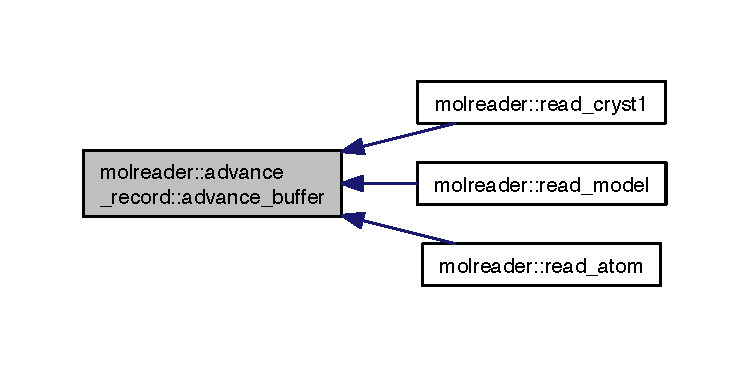
\includegraphics[width=350pt]{interfacemolreader_1_1advance__record_a500888e41a27b357f37c520c1d2a3899_icgraph}
\end{center}
\end{figure}




The documentation for this interface was generated from the following file\+:\begin{DoxyCompactItemize}
\item 
src/\hyperlink{molreader_8f90}{molreader.\+f90}\end{DoxyCompactItemize}

\hypertarget{structmolreader_1_1atom}{\section{molreader\+:\+:atom Type Reference}
\label{structmolreader_1_1atom}\index{molreader\+::atom@{molreader\+::atom}}
}
\subsection*{Private Attributes}
\begin{DoxyCompactItemize}
\item 
character(len=62) \hyperlink{structmolreader_1_1atom_a5f585cc1e6478bed9c81f6fca227f46e}{fmt}
\item 
character(len=\hyperlink{classmolreader_a8f12be3272b946fd698c9fbaf2ba9d32}{reclen}) \hyperlink{structmolreader_1_1atom_ae56449154be2ddb337df3f73dda63d59}{recname}
\item 
integer(long) \hyperlink{structmolreader_1_1atom_a4843d34d24db6a30c5c0c199d4a09cdb}{serial}
\item 
character(len=4) \hyperlink{structmolreader_1_1atom_a2f1818a64010ffcfcd1f90fe07d40233}{name}
\item 
character \hyperlink{structmolreader_1_1atom_a6bed152132fdfceaf62c2627edd94419}{altloc}
\item 
character(len=4) \hyperlink{structmolreader_1_1atom_a67b16254cd2b0ec91772081bd2a8b0ae}{resname}
\item 
character \hyperlink{structmolreader_1_1atom_a40d33bfe323c5ba4969637d03f6f23c1}{chainid}
\item 
integer(long) \hyperlink{structmolreader_1_1atom_ace57beef8994d3c6ec7a5048e66cc4ae}{resseq}
\item 
character \hyperlink{structmolreader_1_1atom_a79a65454286a2c001e4be06ba333220c}{icode}
\item 
real(double) \hyperlink{structmolreader_1_1atom_a2fe09429b1c06d0037917dbc658f599c}{x}
\item 
real(double) \hyperlink{structmolreader_1_1atom_ad723df4b3102cd459daf1896014f5a1e}{y}
\item 
real(double) \hyperlink{structmolreader_1_1atom_ad68c754042ba9fd277d59c6caf9bc570}{z}
\item 
real(double) \hyperlink{structmolreader_1_1atom_a33feec0b246dfe6f38e77b88f1baad7c}{occupancy}
\item 
real(double) \hyperlink{structmolreader_1_1atom_a07cd48fa61d17ae1319fa643fda2b160}{tempfactor}
\item 
character(len=4) \hyperlink{structmolreader_1_1atom_a1a170c779cd77498f491dc7c94115dba}{segname}
\begin{DoxyCompactList}\small\item\em found from some M\+D packages \end{DoxyCompactList}\item 
character(len=2) \hyperlink{structmolreader_1_1atom_a34e74d1598af7abd98aa9323ae538634}{element}
\item 
character(len=2) \hyperlink{structmolreader_1_1atom_a2df0e8e4929647a81fce9d7ce76390cb}{charge}
\end{DoxyCompactItemize}


\subsection{Member Data Documentation}
\hypertarget{structmolreader_1_1atom_a6bed152132fdfceaf62c2627edd94419}{\index{molreader\+::atom@{molreader\+::atom}!altloc@{altloc}}
\index{altloc@{altloc}!molreader\+::atom@{molreader\+::atom}}
\subsubsection[{altloc}]{\setlength{\rightskip}{0pt plus 5cm}character molreader\+::atom\+::altloc\hspace{0.3cm}{\ttfamily [private]}}}\label{structmolreader_1_1atom_a6bed152132fdfceaf62c2627edd94419}
\hypertarget{structmolreader_1_1atom_a40d33bfe323c5ba4969637d03f6f23c1}{\index{molreader\+::atom@{molreader\+::atom}!chainid@{chainid}}
\index{chainid@{chainid}!molreader\+::atom@{molreader\+::atom}}
\subsubsection[{chainid}]{\setlength{\rightskip}{0pt plus 5cm}character molreader\+::atom\+::chainid\hspace{0.3cm}{\ttfamily [private]}}}\label{structmolreader_1_1atom_a40d33bfe323c5ba4969637d03f6f23c1}
\hypertarget{structmolreader_1_1atom_a2df0e8e4929647a81fce9d7ce76390cb}{\index{molreader\+::atom@{molreader\+::atom}!charge@{charge}}
\index{charge@{charge}!molreader\+::atom@{molreader\+::atom}}
\subsubsection[{charge}]{\setlength{\rightskip}{0pt plus 5cm}character(len=2) molreader\+::atom\+::charge\hspace{0.3cm}{\ttfamily [private]}}}\label{structmolreader_1_1atom_a2df0e8e4929647a81fce9d7ce76390cb}
\hypertarget{structmolreader_1_1atom_a34e74d1598af7abd98aa9323ae538634}{\index{molreader\+::atom@{molreader\+::atom}!element@{element}}
\index{element@{element}!molreader\+::atom@{molreader\+::atom}}
\subsubsection[{element}]{\setlength{\rightskip}{0pt plus 5cm}character(len=2) molreader\+::atom\+::element\hspace{0.3cm}{\ttfamily [private]}}}\label{structmolreader_1_1atom_a34e74d1598af7abd98aa9323ae538634}
\hypertarget{structmolreader_1_1atom_a5f585cc1e6478bed9c81f6fca227f46e}{\index{molreader\+::atom@{molreader\+::atom}!fmt@{fmt}}
\index{fmt@{fmt}!molreader\+::atom@{molreader\+::atom}}
\subsubsection[{fmt}]{\setlength{\rightskip}{0pt plus 5cm}character(len=62) molreader\+::atom\+::fmt\hspace{0.3cm}{\ttfamily [private]}}}\label{structmolreader_1_1atom_a5f585cc1e6478bed9c81f6fca227f46e}
\hypertarget{structmolreader_1_1atom_a79a65454286a2c001e4be06ba333220c}{\index{molreader\+::atom@{molreader\+::atom}!icode@{icode}}
\index{icode@{icode}!molreader\+::atom@{molreader\+::atom}}
\subsubsection[{icode}]{\setlength{\rightskip}{0pt plus 5cm}character molreader\+::atom\+::icode\hspace{0.3cm}{\ttfamily [private]}}}\label{structmolreader_1_1atom_a79a65454286a2c001e4be06ba333220c}
\hypertarget{structmolreader_1_1atom_a2f1818a64010ffcfcd1f90fe07d40233}{\index{molreader\+::atom@{molreader\+::atom}!name@{name}}
\index{name@{name}!molreader\+::atom@{molreader\+::atom}}
\subsubsection[{name}]{\setlength{\rightskip}{0pt plus 5cm}character(len=4) molreader\+::atom\+::name\hspace{0.3cm}{\ttfamily [private]}}}\label{structmolreader_1_1atom_a2f1818a64010ffcfcd1f90fe07d40233}
\hypertarget{structmolreader_1_1atom_a33feec0b246dfe6f38e77b88f1baad7c}{\index{molreader\+::atom@{molreader\+::atom}!occupancy@{occupancy}}
\index{occupancy@{occupancy}!molreader\+::atom@{molreader\+::atom}}
\subsubsection[{occupancy}]{\setlength{\rightskip}{0pt plus 5cm}real(double) molreader\+::atom\+::occupancy\hspace{0.3cm}{\ttfamily [private]}}}\label{structmolreader_1_1atom_a33feec0b246dfe6f38e77b88f1baad7c}
\hypertarget{structmolreader_1_1atom_ae56449154be2ddb337df3f73dda63d59}{\index{molreader\+::atom@{molreader\+::atom}!recname@{recname}}
\index{recname@{recname}!molreader\+::atom@{molreader\+::atom}}
\subsubsection[{recname}]{\setlength{\rightskip}{0pt plus 5cm}character(len={\bf reclen}) molreader\+::atom\+::recname\hspace{0.3cm}{\ttfamily [private]}}}\label{structmolreader_1_1atom_ae56449154be2ddb337df3f73dda63d59}
\hypertarget{structmolreader_1_1atom_a67b16254cd2b0ec91772081bd2a8b0ae}{\index{molreader\+::atom@{molreader\+::atom}!resname@{resname}}
\index{resname@{resname}!molreader\+::atom@{molreader\+::atom}}
\subsubsection[{resname}]{\setlength{\rightskip}{0pt plus 5cm}character(len=4) molreader\+::atom\+::resname\hspace{0.3cm}{\ttfamily [private]}}}\label{structmolreader_1_1atom_a67b16254cd2b0ec91772081bd2a8b0ae}
\hypertarget{structmolreader_1_1atom_ace57beef8994d3c6ec7a5048e66cc4ae}{\index{molreader\+::atom@{molreader\+::atom}!resseq@{resseq}}
\index{resseq@{resseq}!molreader\+::atom@{molreader\+::atom}}
\subsubsection[{resseq}]{\setlength{\rightskip}{0pt plus 5cm}integer(long) molreader\+::atom\+::resseq\hspace{0.3cm}{\ttfamily [private]}}}\label{structmolreader_1_1atom_ace57beef8994d3c6ec7a5048e66cc4ae}
\hypertarget{structmolreader_1_1atom_a1a170c779cd77498f491dc7c94115dba}{\index{molreader\+::atom@{molreader\+::atom}!segname@{segname}}
\index{segname@{segname}!molreader\+::atom@{molreader\+::atom}}
\subsubsection[{segname}]{\setlength{\rightskip}{0pt plus 5cm}character(len=4) molreader\+::atom\+::segname\hspace{0.3cm}{\ttfamily [private]}}}\label{structmolreader_1_1atom_a1a170c779cd77498f491dc7c94115dba}


found from some M\+D packages 

\hypertarget{structmolreader_1_1atom_a4843d34d24db6a30c5c0c199d4a09cdb}{\index{molreader\+::atom@{molreader\+::atom}!serial@{serial}}
\index{serial@{serial}!molreader\+::atom@{molreader\+::atom}}
\subsubsection[{serial}]{\setlength{\rightskip}{0pt plus 5cm}integer(long) molreader\+::atom\+::serial\hspace{0.3cm}{\ttfamily [private]}}}\label{structmolreader_1_1atom_a4843d34d24db6a30c5c0c199d4a09cdb}
\hypertarget{structmolreader_1_1atom_a07cd48fa61d17ae1319fa643fda2b160}{\index{molreader\+::atom@{molreader\+::atom}!tempfactor@{tempfactor}}
\index{tempfactor@{tempfactor}!molreader\+::atom@{molreader\+::atom}}
\subsubsection[{tempfactor}]{\setlength{\rightskip}{0pt plus 5cm}real(double) molreader\+::atom\+::tempfactor\hspace{0.3cm}{\ttfamily [private]}}}\label{structmolreader_1_1atom_a07cd48fa61d17ae1319fa643fda2b160}
\hypertarget{structmolreader_1_1atom_a2fe09429b1c06d0037917dbc658f599c}{\index{molreader\+::atom@{molreader\+::atom}!x@{x}}
\index{x@{x}!molreader\+::atom@{molreader\+::atom}}
\subsubsection[{x}]{\setlength{\rightskip}{0pt plus 5cm}real(double) molreader\+::atom\+::x\hspace{0.3cm}{\ttfamily [private]}}}\label{structmolreader_1_1atom_a2fe09429b1c06d0037917dbc658f599c}
\hypertarget{structmolreader_1_1atom_ad723df4b3102cd459daf1896014f5a1e}{\index{molreader\+::atom@{molreader\+::atom}!y@{y}}
\index{y@{y}!molreader\+::atom@{molreader\+::atom}}
\subsubsection[{y}]{\setlength{\rightskip}{0pt plus 5cm}real(double) molreader\+::atom\+::y\hspace{0.3cm}{\ttfamily [private]}}}\label{structmolreader_1_1atom_ad723df4b3102cd459daf1896014f5a1e}
\hypertarget{structmolreader_1_1atom_ad68c754042ba9fd277d59c6caf9bc570}{\index{molreader\+::atom@{molreader\+::atom}!z@{z}}
\index{z@{z}!molreader\+::atom@{molreader\+::atom}}
\subsubsection[{z}]{\setlength{\rightskip}{0pt plus 5cm}real(double) molreader\+::atom\+::z\hspace{0.3cm}{\ttfamily [private]}}}\label{structmolreader_1_1atom_ad68c754042ba9fd277d59c6caf9bc570}


The documentation for this type was generated from the following file\+:\begin{DoxyCompactItemize}
\item 
src/\hyperlink{molreader_8f90}{molreader.\+f90}\end{DoxyCompactItemize}

\hypertarget{classatomicunits}{\section{atomicunits Module Reference}
\label{classatomicunits}\index{atomicunits@{atomicunits}}
}


Definition of atomic units.  


\subsection*{Public Attributes}
\begin{DoxyCompactItemize}
\item 
real(double), parameter \hyperlink{classatomicunits_aa4859dbb9e7739ae603b78d9f2c58f93}{a0}
\begin{DoxyCompactList}\small\item\em (Fundamental length) Bohr radius \end{DoxyCompactList}\item 
real(double), parameter \hyperlink{classatomicunits_a02f36d49c4a56d1cc84c8cda6c631a68}{me}
\begin{DoxyCompactList}\small\item\em (Fundamental mass) electron mass \end{DoxyCompactList}\item 
real(double), parameter \hyperlink{classatomicunits_a7dffaade5d28d129a3726e8eff794447}{hbar}
\begin{DoxyCompactList}\small\item\em (Fundamental action) reduced Planks const \end{DoxyCompactList}\item 
real(double), parameter \hyperlink{classatomicunits_af3650eaf423c8af5e887256a5e8023d6}{e}
\begin{DoxyCompactList}\small\item\em (Fundamental charge) electron charge \end{DoxyCompactList}\item 
real(double), parameter \hyperlink{classatomicunits_a0b4d6ac453558bc86022587236f7d076}{kel}
\begin{DoxyCompactList}\small\item\em (Fundamental temperature) Kelvin \end{DoxyCompactList}\item 
real(double), parameter \hyperlink{classatomicunits_af00d60f8fc301784d6e48a53e524a4c8}{mol}
\begin{DoxyCompactList}\small\item\em (Fundamental amount) Avogadro's number \end{DoxyCompactList}\item 
real(double), parameter \hyperlink{classatomicunits_a07ac069b1a5417fd61aa3954d6b66d83}{rad}
\begin{DoxyCompactList}\small\item\em (Fundamental angle) radian \end{DoxyCompactList}\item 
real(double), parameter \hyperlink{classatomicunits_a39b85d20ed96ab0b9dfb86c7646a61a0}{eh}
\begin{DoxyCompactList}\small\item\em Hartree (unit value) \end{DoxyCompactList}\item 
real(double), parameter \hyperlink{classatomicunits_aafc175708d34f52459448530cdec9aae}{kc}
\begin{DoxyCompactList}\small\item\em Coulomb force (unit value) \end{DoxyCompactList}\item 
real(double), parameter \hyperlink{classatomicunits_a62f37608529c74a442a81baa515965d6}{mp}
\begin{DoxyCompactList}\small\item\em proton rest mass \end{DoxyCompactList}\item 
real(double), parameter \hyperlink{classatomicunits_a001e0a01ab152644eb7df31ade44b290}{mn}
\begin{DoxyCompactList}\small\item\em neutron rest mass \end{DoxyCompactList}\item 
real(double), parameter \hyperlink{classatomicunits_afe876defe82137d91908691c6765a5f1}{kb}
\begin{DoxyCompactList}\small\item\em boltzman constant \end{DoxyCompactList}\item 
real(double), parameter \hyperlink{classatomicunits_a10a69964ce0d082d71ee5ae34a5a0d24}{ev}
\begin{DoxyCompactList}\small\item\em Electon volt. \end{DoxyCompactList}\item 
real(double), parameter \hyperlink{classatomicunits_ae35b35bfa15b571da842371a32dcb2e6}{c0}
\begin{DoxyCompactList}\small\item\em speed of light \end{DoxyCompactList}\item 
real(double), parameter \hyperlink{classatomicunits_a45821c6127c356d71ba94bf34b962653}{eps0}
\begin{DoxyCompactList}\small\item\em vacuum permittivity \end{DoxyCompactList}\item 
real(double), parameter \hyperlink{classatomicunits_af82c72bfababde1e5da6ac04a43b8570}{debye}
\begin{DoxyCompactList}\small\item\em Dipole moment. \end{DoxyCompactList}\item 
real(double), parameter \hyperlink{classatomicunits_af9552fc54f3050b11cce6152261c2bf2}{deg}
\begin{DoxyCompactList}\small\item\em Degrees. \end{DoxyCompactList}\item 
real(double), parameter \hyperlink{classatomicunits_a618f9dcd7de9b9ddb53af5bd4f1095c6}{angstrom}
\begin{DoxyCompactList}\small\item\em angstrom \end{DoxyCompactList}\item 
real(double), parameter \hyperlink{classatomicunits_a51f9c61f64f3aec674dd6dbb342e733d}{fs}
\begin{DoxyCompactList}\small\item\em femtosecond \end{DoxyCompactList}\item 
real(double), parameter \hyperlink{classatomicunits_af5dac3bb123ac05a538d6ebd2373eb3b}{ps}
\begin{DoxyCompactList}\small\item\em picosecond \end{DoxyCompactList}\item 
real(double), parameter \hyperlink{classatomicunits_a1741cd0f8cdd696033c1c18531740795}{invcm}
\begin{DoxyCompactList}\small\item\em wavenumber(1/cm) \end{DoxyCompactList}\end{DoxyCompactItemize}


\subsection{Detailed Description}
Definition of atomic units. 

Atomic units are the default used throughout the software. \begin{DoxyAuthor}{Author}
Daniel Montemayor 
\end{DoxyAuthor}


\subsection{Member Data Documentation}
\hypertarget{classatomicunits_aa4859dbb9e7739ae603b78d9f2c58f93}{\index{atomicunits@{atomicunits}!a0@{a0}}
\index{a0@{a0}!atomicunits@{atomicunits}}
\subsubsection[{a0}]{\setlength{\rightskip}{0pt plus 5cm}real(double), parameter atomicunits\+::a0}}\label{classatomicunits_aa4859dbb9e7739ae603b78d9f2c58f93}


(Fundamental length) Bohr radius 

\hypertarget{classatomicunits_a618f9dcd7de9b9ddb53af5bd4f1095c6}{\index{atomicunits@{atomicunits}!angstrom@{angstrom}}
\index{angstrom@{angstrom}!atomicunits@{atomicunits}}
\subsubsection[{angstrom}]{\setlength{\rightskip}{0pt plus 5cm}real(double), parameter atomicunits\+::angstrom}}\label{classatomicunits_a618f9dcd7de9b9ddb53af5bd4f1095c6}


angstrom 

\hypertarget{classatomicunits_ae35b35bfa15b571da842371a32dcb2e6}{\index{atomicunits@{atomicunits}!c0@{c0}}
\index{c0@{c0}!atomicunits@{atomicunits}}
\subsubsection[{c0}]{\setlength{\rightskip}{0pt plus 5cm}real(double), parameter atomicunits\+::c0}}\label{classatomicunits_ae35b35bfa15b571da842371a32dcb2e6}


speed of light 

\hypertarget{classatomicunits_af82c72bfababde1e5da6ac04a43b8570}{\index{atomicunits@{atomicunits}!debye@{debye}}
\index{debye@{debye}!atomicunits@{atomicunits}}
\subsubsection[{debye}]{\setlength{\rightskip}{0pt plus 5cm}real(double), parameter atomicunits\+::debye}}\label{classatomicunits_af82c72bfababde1e5da6ac04a43b8570}


Dipole moment. 

\hypertarget{classatomicunits_af9552fc54f3050b11cce6152261c2bf2}{\index{atomicunits@{atomicunits}!deg@{deg}}
\index{deg@{deg}!atomicunits@{atomicunits}}
\subsubsection[{deg}]{\setlength{\rightskip}{0pt plus 5cm}real(double), parameter atomicunits\+::deg}}\label{classatomicunits_af9552fc54f3050b11cce6152261c2bf2}


Degrees. 

\hypertarget{classatomicunits_af3650eaf423c8af5e887256a5e8023d6}{\index{atomicunits@{atomicunits}!e@{e}}
\index{e@{e}!atomicunits@{atomicunits}}
\subsubsection[{e}]{\setlength{\rightskip}{0pt plus 5cm}real(double), parameter atomicunits\+::e}}\label{classatomicunits_af3650eaf423c8af5e887256a5e8023d6}


(Fundamental charge) electron charge 

\hypertarget{classatomicunits_a39b85d20ed96ab0b9dfb86c7646a61a0}{\index{atomicunits@{atomicunits}!eh@{eh}}
\index{eh@{eh}!atomicunits@{atomicunits}}
\subsubsection[{eh}]{\setlength{\rightskip}{0pt plus 5cm}real(double), parameter atomicunits\+::eh}}\label{classatomicunits_a39b85d20ed96ab0b9dfb86c7646a61a0}


Hartree (unit value) 

\hypertarget{classatomicunits_a45821c6127c356d71ba94bf34b962653}{\index{atomicunits@{atomicunits}!eps0@{eps0}}
\index{eps0@{eps0}!atomicunits@{atomicunits}}
\subsubsection[{eps0}]{\setlength{\rightskip}{0pt plus 5cm}real(double), parameter atomicunits\+::eps0}}\label{classatomicunits_a45821c6127c356d71ba94bf34b962653}


vacuum permittivity 

\hypertarget{classatomicunits_a10a69964ce0d082d71ee5ae34a5a0d24}{\index{atomicunits@{atomicunits}!ev@{ev}}
\index{ev@{ev}!atomicunits@{atomicunits}}
\subsubsection[{ev}]{\setlength{\rightskip}{0pt plus 5cm}real(double), parameter atomicunits\+::ev}}\label{classatomicunits_a10a69964ce0d082d71ee5ae34a5a0d24}


Electon volt. 

\hypertarget{classatomicunits_a51f9c61f64f3aec674dd6dbb342e733d}{\index{atomicunits@{atomicunits}!fs@{fs}}
\index{fs@{fs}!atomicunits@{atomicunits}}
\subsubsection[{fs}]{\setlength{\rightskip}{0pt plus 5cm}real(double), parameter atomicunits\+::fs}}\label{classatomicunits_a51f9c61f64f3aec674dd6dbb342e733d}


femtosecond 

\hypertarget{classatomicunits_a7dffaade5d28d129a3726e8eff794447}{\index{atomicunits@{atomicunits}!hbar@{hbar}}
\index{hbar@{hbar}!atomicunits@{atomicunits}}
\subsubsection[{hbar}]{\setlength{\rightskip}{0pt plus 5cm}real(double), parameter atomicunits\+::hbar}}\label{classatomicunits_a7dffaade5d28d129a3726e8eff794447}


(Fundamental action) reduced Planks const 

\hypertarget{classatomicunits_a1741cd0f8cdd696033c1c18531740795}{\index{atomicunits@{atomicunits}!invcm@{invcm}}
\index{invcm@{invcm}!atomicunits@{atomicunits}}
\subsubsection[{invcm}]{\setlength{\rightskip}{0pt plus 5cm}real(double), parameter atomicunits\+::invcm}}\label{classatomicunits_a1741cd0f8cdd696033c1c18531740795}


wavenumber(1/cm) 

\hypertarget{classatomicunits_afe876defe82137d91908691c6765a5f1}{\index{atomicunits@{atomicunits}!kb@{kb}}
\index{kb@{kb}!atomicunits@{atomicunits}}
\subsubsection[{kb}]{\setlength{\rightskip}{0pt plus 5cm}real(double), parameter atomicunits\+::kb}}\label{classatomicunits_afe876defe82137d91908691c6765a5f1}


boltzman constant 

\hypertarget{classatomicunits_aafc175708d34f52459448530cdec9aae}{\index{atomicunits@{atomicunits}!kc@{kc}}
\index{kc@{kc}!atomicunits@{atomicunits}}
\subsubsection[{kc}]{\setlength{\rightskip}{0pt plus 5cm}real(double), parameter atomicunits\+::kc}}\label{classatomicunits_aafc175708d34f52459448530cdec9aae}


Coulomb force (unit value) 

\hypertarget{classatomicunits_a0b4d6ac453558bc86022587236f7d076}{\index{atomicunits@{atomicunits}!kel@{kel}}
\index{kel@{kel}!atomicunits@{atomicunits}}
\subsubsection[{kel}]{\setlength{\rightskip}{0pt plus 5cm}real(double), parameter atomicunits\+::kel}}\label{classatomicunits_a0b4d6ac453558bc86022587236f7d076}


(Fundamental temperature) Kelvin 

\hypertarget{classatomicunits_a02f36d49c4a56d1cc84c8cda6c631a68}{\index{atomicunits@{atomicunits}!me@{me}}
\index{me@{me}!atomicunits@{atomicunits}}
\subsubsection[{me}]{\setlength{\rightskip}{0pt plus 5cm}real(double), parameter atomicunits\+::me}}\label{classatomicunits_a02f36d49c4a56d1cc84c8cda6c631a68}


(Fundamental mass) electron mass 

\hypertarget{classatomicunits_a001e0a01ab152644eb7df31ade44b290}{\index{atomicunits@{atomicunits}!mn@{mn}}
\index{mn@{mn}!atomicunits@{atomicunits}}
\subsubsection[{mn}]{\setlength{\rightskip}{0pt plus 5cm}real(double), parameter atomicunits\+::mn}}\label{classatomicunits_a001e0a01ab152644eb7df31ade44b290}


neutron rest mass 

\hypertarget{classatomicunits_af00d60f8fc301784d6e48a53e524a4c8}{\index{atomicunits@{atomicunits}!mol@{mol}}
\index{mol@{mol}!atomicunits@{atomicunits}}
\subsubsection[{mol}]{\setlength{\rightskip}{0pt plus 5cm}real(double), parameter atomicunits\+::mol}}\label{classatomicunits_af00d60f8fc301784d6e48a53e524a4c8}


(Fundamental amount) Avogadro's number 

\hypertarget{classatomicunits_a62f37608529c74a442a81baa515965d6}{\index{atomicunits@{atomicunits}!mp@{mp}}
\index{mp@{mp}!atomicunits@{atomicunits}}
\subsubsection[{mp}]{\setlength{\rightskip}{0pt plus 5cm}real(double), parameter atomicunits\+::mp}}\label{classatomicunits_a62f37608529c74a442a81baa515965d6}


proton rest mass 

\hypertarget{classatomicunits_af5dac3bb123ac05a538d6ebd2373eb3b}{\index{atomicunits@{atomicunits}!ps@{ps}}
\index{ps@{ps}!atomicunits@{atomicunits}}
\subsubsection[{ps}]{\setlength{\rightskip}{0pt plus 5cm}real(double), parameter atomicunits\+::ps}}\label{classatomicunits_af5dac3bb123ac05a538d6ebd2373eb3b}


picosecond 

\hypertarget{classatomicunits_a07ac069b1a5417fd61aa3954d6b66d83}{\index{atomicunits@{atomicunits}!rad@{rad}}
\index{rad@{rad}!atomicunits@{atomicunits}}
\subsubsection[{rad}]{\setlength{\rightskip}{0pt plus 5cm}real(double), parameter atomicunits\+::rad}}\label{classatomicunits_a07ac069b1a5417fd61aa3954d6b66d83}


(Fundamental angle) radian 



The documentation for this module was generated from the following file\+:\begin{DoxyCompactItemize}
\item 
src/\hyperlink{utils_8f90}{utils.\+f90}\end{DoxyCompactItemize}

\hypertarget{structbilinear__class_1_1bilinear}{}\section{bilinear\+\_\+class\+:\+:bilinear Type Reference}
\label{structbilinear__class_1_1bilinear}\index{bilinear\+\_\+class\+::bilinear@{bilinear\+\_\+class\+::bilinear}}


Derived quantum-\/classical coupling term.  




Collaboration diagram for bilinear\+\_\+class\+:\+:bilinear\+:\nopagebreak
\begin{figure}[H]
\begin{center}
\leavevmode
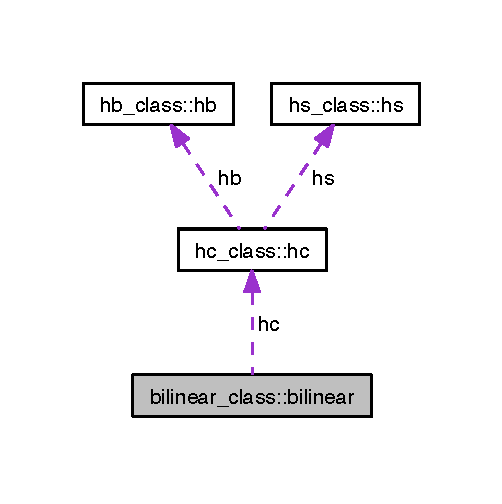
\includegraphics[width=241pt]{structbilinear__class_1_1bilinear__coll__graph}
\end{center}
\end{figure}
\subsection*{Private Attributes}
\begin{DoxyCompactItemize}
\item 
logical \hyperlink{structbilinear__class_1_1bilinear_a97bca767cbc1ecae9489db5950da06bc}{initialized}
\begin{DoxyCompactList}\small\item\em True if coupling term has been properly initialized. \end{DoxyCompactList}\item 
type(\hyperlink{structhc__class_1_1hc}{hc}) \hyperlink{structbilinear__class_1_1bilinear_aeb9f98e320b690f4bfef83caf407dfaa}{hc}
\begin{DoxyCompactList}\small\item\em Inherited coupling primitive type. \end{DoxyCompactList}\item 
real(double), dimension(\+:), pointer \hyperlink{structbilinear__class_1_1bilinear_aabd615d49d52220aac52707b2e2b1aa6}{lambda}
\begin{DoxyCompactList}\small\item\em Array containing the vaules of the bath reorganization energy about each state and has dimensions (qs.\+hs.\+nstate). \end{DoxyCompactList}\item 
integer(long), dimension(\+:), pointer \hyperlink{structbilinear__class_1_1bilinear_a78e65d82cd358d5dfa19b780ab877fa0}{bdof}
\begin{DoxyCompactList}\small\item\em Number of dissipative bath modes associated to each state has dimensions (qs.\+hs.\+nstate). \end{DoxyCompactList}\item 
real(double), dimension(\+:,\+:), pointer \hyperlink{structbilinear__class_1_1bilinear_a910401429e7649dba49acbab872a1b75}{g}
\begin{DoxyCompactList}\small\item\em Coefficient coupling each quantum state to the normal modes of the classical subsystem. \end{DoxyCompactList}\item 
real(double), dimension(\+:), pointer \hyperlink{structbilinear__class_1_1bilinear_a809699845e36e344b7aeb51642c333ec}{f}
\begin{DoxyCompactList}\small\item\em Eigen values of the $ \hat q $ operator. The native diabatic basis states are assumed eigen states of the $ \hat q $ operator with eigen values stored in the array f of dimension (qs.\+hs.\+nstate). \end{DoxyCompactList}\item 
logical, dimension(\+:,\+:), pointer \hyperlink{structbilinear__class_1_1bilinear_aeb06e78f97c5cdac0c83422ec087e2e0}{gmap}
\item 
logical \hyperlink{structbilinear__class_1_1bilinear_a78eec2ff8a3e1de38eb02ceeb108ad15}{wbasis}
\item 
logical \hyperlink{structbilinear__class_1_1bilinear_aba7556e23595f003ffcf20327dc18f3e}{ctused}
\end{DoxyCompactItemize}


\subsection{Detailed Description}
Derived quantum-\/classical coupling term. 

\subsection{Member Data Documentation}
\mbox{\Hypertarget{structbilinear__class_1_1bilinear_a78e65d82cd358d5dfa19b780ab877fa0}\label{structbilinear__class_1_1bilinear_a78e65d82cd358d5dfa19b780ab877fa0}} 
\index{bilinear\+\_\+class\+::bilinear@{bilinear\+\_\+class\+::bilinear}!bdof@{bdof}}
\index{bdof@{bdof}!bilinear\+\_\+class\+::bilinear@{bilinear\+\_\+class\+::bilinear}}
\subsubsection{\texorpdfstring{bdof}{bdof}}
{\footnotesize\ttfamily integer(long), dimension(\+:), pointer bilinear\+\_\+class\+::bilinear\+::bdof\hspace{0.3cm}{\ttfamily [private]}}



Number of dissipative bath modes associated to each state has dimensions (qs.\+hs.\+nstate). 

\mbox{\Hypertarget{structbilinear__class_1_1bilinear_aba7556e23595f003ffcf20327dc18f3e}\label{structbilinear__class_1_1bilinear_aba7556e23595f003ffcf20327dc18f3e}} 
\index{bilinear\+\_\+class\+::bilinear@{bilinear\+\_\+class\+::bilinear}!ctused@{ctused}}
\index{ctused@{ctused}!bilinear\+\_\+class\+::bilinear@{bilinear\+\_\+class\+::bilinear}}
\subsubsection{\texorpdfstring{ctused}{ctused}}
{\footnotesize\ttfamily logical bilinear\+\_\+class\+::bilinear\+::ctused\hspace{0.3cm}{\ttfamily [private]}}

\mbox{\Hypertarget{structbilinear__class_1_1bilinear_a809699845e36e344b7aeb51642c333ec}\label{structbilinear__class_1_1bilinear_a809699845e36e344b7aeb51642c333ec}} 
\index{bilinear\+\_\+class\+::bilinear@{bilinear\+\_\+class\+::bilinear}!f@{f}}
\index{f@{f}!bilinear\+\_\+class\+::bilinear@{bilinear\+\_\+class\+::bilinear}}
\subsubsection{\texorpdfstring{f}{f}}
{\footnotesize\ttfamily real(double), dimension(\+:), pointer bilinear\+\_\+class\+::bilinear\+::f\hspace{0.3cm}{\ttfamily [private]}}



Eigen values of the $ \hat q $ operator. The native diabatic basis states are assumed eigen states of the $ \hat q $ operator with eigen values stored in the array f of dimension (qs.\+hs.\+nstate). 

\mbox{\Hypertarget{structbilinear__class_1_1bilinear_a910401429e7649dba49acbab872a1b75}\label{structbilinear__class_1_1bilinear_a910401429e7649dba49acbab872a1b75}} 
\index{bilinear\+\_\+class\+::bilinear@{bilinear\+\_\+class\+::bilinear}!g@{g}}
\index{g@{g}!bilinear\+\_\+class\+::bilinear@{bilinear\+\_\+class\+::bilinear}}
\subsubsection{\texorpdfstring{g}{g}}
{\footnotesize\ttfamily real(double), dimension(\+:,\+:), pointer bilinear\+\_\+class\+::bilinear\+::g\hspace{0.3cm}{\ttfamily [private]}}



Coefficient coupling each quantum state to the normal modes of the classical subsystem. 

\mbox{\Hypertarget{structbilinear__class_1_1bilinear_aeb06e78f97c5cdac0c83422ec087e2e0}\label{structbilinear__class_1_1bilinear_aeb06e78f97c5cdac0c83422ec087e2e0}} 
\index{bilinear\+\_\+class\+::bilinear@{bilinear\+\_\+class\+::bilinear}!gmap@{gmap}}
\index{gmap@{gmap}!bilinear\+\_\+class\+::bilinear@{bilinear\+\_\+class\+::bilinear}}
\subsubsection{\texorpdfstring{gmap}{gmap}}
{\footnotesize\ttfamily logical, dimension(\+:,\+:), pointer bilinear\+\_\+class\+::bilinear\+::gmap\hspace{0.3cm}{\ttfamily [private]}}

\mbox{\Hypertarget{structbilinear__class_1_1bilinear_aeb9f98e320b690f4bfef83caf407dfaa}\label{structbilinear__class_1_1bilinear_aeb9f98e320b690f4bfef83caf407dfaa}} 
\index{bilinear\+\_\+class\+::bilinear@{bilinear\+\_\+class\+::bilinear}!hc@{hc}}
\index{hc@{hc}!bilinear\+\_\+class\+::bilinear@{bilinear\+\_\+class\+::bilinear}}
\subsubsection{\texorpdfstring{hc}{hc}}
{\footnotesize\ttfamily type(\hyperlink{structhc__class_1_1hc}{hc}) bilinear\+\_\+class\+::bilinear\+::hc\hspace{0.3cm}{\ttfamily [private]}}



Inherited coupling primitive type. 

\mbox{\Hypertarget{structbilinear__class_1_1bilinear_a97bca767cbc1ecae9489db5950da06bc}\label{structbilinear__class_1_1bilinear_a97bca767cbc1ecae9489db5950da06bc}} 
\index{bilinear\+\_\+class\+::bilinear@{bilinear\+\_\+class\+::bilinear}!initialized@{initialized}}
\index{initialized@{initialized}!bilinear\+\_\+class\+::bilinear@{bilinear\+\_\+class\+::bilinear}}
\subsubsection{\texorpdfstring{initialized}{initialized}}
{\footnotesize\ttfamily logical bilinear\+\_\+class\+::bilinear\+::initialized\hspace{0.3cm}{\ttfamily [private]}}



True if coupling term has been properly initialized. 

\mbox{\Hypertarget{structbilinear__class_1_1bilinear_aabd615d49d52220aac52707b2e2b1aa6}\label{structbilinear__class_1_1bilinear_aabd615d49d52220aac52707b2e2b1aa6}} 
\index{bilinear\+\_\+class\+::bilinear@{bilinear\+\_\+class\+::bilinear}!lambda@{lambda}}
\index{lambda@{lambda}!bilinear\+\_\+class\+::bilinear@{bilinear\+\_\+class\+::bilinear}}
\subsubsection{\texorpdfstring{lambda}{lambda}}
{\footnotesize\ttfamily real(double), dimension(\+:), pointer bilinear\+\_\+class\+::bilinear\+::lambda\hspace{0.3cm}{\ttfamily [private]}}



Array containing the vaules of the bath reorganization energy about each state and has dimensions (qs.\+hs.\+nstate). 

\mbox{\Hypertarget{structbilinear__class_1_1bilinear_a78eec2ff8a3e1de38eb02ceeb108ad15}\label{structbilinear__class_1_1bilinear_a78eec2ff8a3e1de38eb02ceeb108ad15}} 
\index{bilinear\+\_\+class\+::bilinear@{bilinear\+\_\+class\+::bilinear}!wbasis@{wbasis}}
\index{wbasis@{wbasis}!bilinear\+\_\+class\+::bilinear@{bilinear\+\_\+class\+::bilinear}}
\subsubsection{\texorpdfstring{wbasis}{wbasis}}
{\footnotesize\ttfamily logical bilinear\+\_\+class\+::bilinear\+::wbasis\hspace{0.3cm}{\ttfamily [private]}}



The documentation for this type was generated from the following file\+:\begin{DoxyCompactItemize}
\item 
src/\hyperlink{bilinear_8f90}{bilinear.\+f90}\end{DoxyCompactItemize}

\hypertarget{classbilinear__class}{\section{bilinear\-\_\-class Module Reference}
\label{classbilinear__class}\index{bilinear\-\_\-class@{bilinear\-\_\-class}}
}


Diagonal Bi-\/linear system-\/bath coupling.  


\subsection*{Data Types}
\begin{DoxyCompactItemize}
\item 
type \hyperlink{structbilinear__class_1_1bilinear}{bilinear}
\begin{DoxyCompactList}\small\item\em Derived quantum-\/classical coupling term. \end{DoxyCompactList}\item 
interface \hyperlink{interfacebilinear__class_1_1check}{check}
\begin{DoxyCompactList}\small\item\em Checks the bilinear object. \end{DoxyCompactList}\item 
interface \hyperlink{interfacebilinear__class_1_1display}{display}
\begin{DoxyCompactList}\small\item\em Displays the current state of the bilinear object. \end{DoxyCompactList}\item 
interface \hyperlink{interfacebilinear__class_1_1kill}{kill}
\begin{DoxyCompactList}\small\item\em Destroys the bilinear object. \end{DoxyCompactList}\item 
interface \hyperlink{interfacebilinear__class_1_1new}{new}
\begin{DoxyCompactList}\small\item\em Creates the bilinear object. \end{DoxyCompactList}\item 
interface \hyperlink{interfacebilinear__class_1_1resample}{resample}
\begin{DoxyCompactList}\small\item\em Reinitializes the bilinear object. \end{DoxyCompactList}\item 
interface \hyperlink{interfacebilinear__class_1_1save}{save}
\begin{DoxyCompactList}\small\item\em Saves the current state of the bilinear object to file. \end{DoxyCompactList}\item 
interface \hyperlink{interfacebilinear__class_1_1update}{update}
\begin{DoxyCompactList}\small\item\em Recalculates bilinear object. \end{DoxyCompactList}\end{DoxyCompactItemize}
\subsection*{Private Member Functions}
\begin{DoxyCompactItemize}
\item 
subroutine \hyperlink{classbilinear__class_a767f35cd3ebd5ef00f6a55fd775c3a27}{bilinear\-\_\-init} (this, qs, cs, file)
\begin{DoxyCompactList}\small\item\em Creates and initializes the bilinear coupling object. \end{DoxyCompactList}\item 
subroutine \hyperlink{classbilinear__class_ae206ab58d224c9a0b7e25ac038e003ae}{bilinear\-\_\-kill} (this)
\begin{DoxyCompactList}\small\item\em Destroys the bilinear coupling object. \end{DoxyCompactList}\item 
subroutine \hyperlink{classbilinear__class_a37ead815723c4c247c156200f5bf4721}{bilinear\-\_\-update} (this)
\begin{DoxyCompactList}\small\item\em Computes the current state of bilinear coupling object. \end{DoxyCompactList}\item 
subroutine \hyperlink{classbilinear__class_aac587f5ea6d66ee89ff3210b10569777}{bilinear\-\_\-resample} (this)
\begin{DoxyCompactList}\small\item\em Re-\/initiallizes the bilinear coupling object. \end{DoxyCompactList}\item 
subroutine \hyperlink{classbilinear__class_a5fe875f5d4db31ef7a7e721ba4a0146a}{bilinear\-\_\-save} (this, file)
\begin{DoxyCompactList}\small\item\em Saves the current state of the bilinear coupling object to file. \end{DoxyCompactList}\item 
subroutine \hyperlink{classbilinear__class_a4346246df7738e0d609716d961a3b94c}{bilinear\-\_\-display} (this, msg)
\begin{DoxyCompactList}\small\item\em Displays the bilinear coupling object. \end{DoxyCompactList}\item 
integer(short) function \hyperlink{classbilinear__class_ab2484d90163983597fb17b15e480e675}{bilinear\-\_\-check} (this)
\begin{DoxyCompactList}\small\item\em Checks the bilinear coupling object. \end{DoxyCompactList}\end{DoxyCompactItemize}


\subsection{Detailed Description}
Diagonal Bi-\/linear system-\/bath coupling. 

This coupling scheme follows the Caldeira-\/\-Leggett model, coupling the normal modes of the classical subsystem linearly to the diagonal states of the quantum subsystem. Assumes Hamiltonian of the form \[ H=h_s+h_b+h_c+ct \] where the quantum subsystem Hamiltonian matrix elements $ \langle\psi_i|hs|\psi_j\rangle $ are the matrix elements of $qs.hs.diabats$. The classical subsystem $ hb $ potential energy ,is written in terms of the normal modes of the classical subsystem $cs.hb.W$. Each one of the $ N$ states is coupled to one or more of the $ K $ normal modes. Here we assume that the diabatic basis states $ \psi $ are eigenstates of some quantum subsystem operator $ \hat q $ such that \[ \hat q |\psi_j\rangle =f_j|\psi_j\rangle \] and the eigenvalues $ f_j $ are supplied by the user. The bilinear coupling term is written \[ h_c=-\sum_n^N \sum_k^{K_n} g_{k,n} Q_{k} f_n |\psi_n\rangle\langle\psi_n|\] with counter term \[ ct=\sum_n^N \sum_k^{K_n} \frac{g_{k,n}^2}{2m_{k}\omega_{k}^2}f_n^2 |\psi_n\rangle\langle\psi_n|. \] The coefficients $ g_{k,n} $ are sampled from the spectral density $ J_n(\omega)$ describing the solvent response about the state $ n $. The spectral density is written \[ J_n(\omega)=\frac{\pi}{\hbar}\sum_k^{K_n}\frac{g_{k,n}^2}{2m_{k,n}\omega_{k,n}}\delta_{\omega-\omega_{k,n}}.\] The re-\/organization energy for each state is defined \[ \lambda_n=\frac{1}{\pi} \int_0^\infty \frac{J_n(\omega)}{\omega} d\omega \] such that, \[ g_{k,n}^2=\frac{2\lambda_n m_{k} \omega_{k}^2}{K_n}\] and \[ ct=\sum_n^N \lambda_n f_n^2|\psi_n\rangle\langle\psi_n| .\] \begin{DoxyAuthor}{Authors}
Daniel Montemayor
\end{DoxyAuthor}
\begin{DoxyDate}{Date}
Aug 2011, Sept 2011, Oct 2012 ,Feb 2013 
\end{DoxyDate}


\subsection{Member Function/\-Subroutine Documentation}
\hypertarget{classbilinear__class_ab2484d90163983597fb17b15e480e675}{\index{bilinear\-\_\-class@{bilinear\-\_\-class}!bilinear\-\_\-check@{bilinear\-\_\-check}}
\index{bilinear\-\_\-check@{bilinear\-\_\-check}!bilinear_class@{bilinear\-\_\-class}}
\subsubsection[{bilinear\-\_\-check}]{\setlength{\rightskip}{0pt plus 5cm}integer(short) function bilinear\-\_\-class\-::bilinear\-\_\-check (
\begin{DoxyParamCaption}
\item[{type({\bf bilinear}), intent(in)}]{this}
\end{DoxyParamCaption}
)\hspace{0.3cm}{\ttfamily [private]}}}\label{classbilinear__class_ab2484d90163983597fb17b15e480e675}


Checks the bilinear coupling object. 


\begin{DoxyParams}[1]{Parameters}
\mbox{\tt in}  & {\em this} & is the bilinear coupling object to be updated. \\
\hline
\mbox{\tt in}  & {\em msg} & is an optional string message to preface the displayed object. \\
\hline
\mbox{\tt in}  & {\em file} & is an optional string containing the location of a file where the display output gets forwarded. \\
\hline
\end{DoxyParams}


Here is the call graph for this function\-:
\nopagebreak
\begin{figure}[H]
\begin{center}
\leavevmode
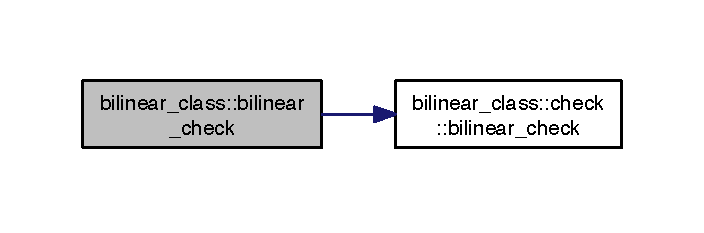
\includegraphics[width=338pt]{classbilinear__class_ab2484d90163983597fb17b15e480e675_cgraph}
\end{center}
\end{figure}


\hypertarget{classbilinear__class_a4346246df7738e0d609716d961a3b94c}{\index{bilinear\-\_\-class@{bilinear\-\_\-class}!bilinear\-\_\-display@{bilinear\-\_\-display}}
\index{bilinear\-\_\-display@{bilinear\-\_\-display}!bilinear_class@{bilinear\-\_\-class}}
\subsubsection[{bilinear\-\_\-display}]{\setlength{\rightskip}{0pt plus 5cm}subroutine bilinear\-\_\-class\-::bilinear\-\_\-display (
\begin{DoxyParamCaption}
\item[{type({\bf bilinear}), intent(in)}]{this, }
\item[{character$\ast$($\ast$), intent(in), optional}]{msg}
\end{DoxyParamCaption}
)\hspace{0.3cm}{\ttfamily [private]}}}\label{classbilinear__class_a4346246df7738e0d609716d961a3b94c}


Displays the bilinear coupling object. 


\begin{DoxyParams}[1]{Parameters}
\mbox{\tt in}  & {\em this} & is the bilinear coupling object to be checked. \\
\hline
\end{DoxyParams}
\begin{DoxyReturn}{Returns}
Nothing if all checks pass or 1 and a warn for the first failed check. 
\end{DoxyReturn}
\begin{DoxyRemark}{Remarks}
Will exit after first failed check. 
\end{DoxyRemark}
\hypertarget{classbilinear__class_a767f35cd3ebd5ef00f6a55fd775c3a27}{\index{bilinear\-\_\-class@{bilinear\-\_\-class}!bilinear\-\_\-init@{bilinear\-\_\-init}}
\index{bilinear\-\_\-init@{bilinear\-\_\-init}!bilinear_class@{bilinear\-\_\-class}}
\subsubsection[{bilinear\-\_\-init}]{\setlength{\rightskip}{0pt plus 5cm}subroutine bilinear\-\_\-class\-::bilinear\-\_\-init (
\begin{DoxyParamCaption}
\item[{type({\bf bilinear}), intent(inout)}]{this, }
\item[{type(quantum), intent(inout), target}]{qs, }
\item[{type(classical), intent(inout), target}]{cs, }
\item[{character$\ast$($\ast$), intent(in), optional}]{file}
\end{DoxyParamCaption}
)\hspace{0.3cm}{\ttfamily [private]}}}\label{classbilinear__class_a767f35cd3ebd5ef00f6a55fd775c3a27}


Creates and initializes the bilinear coupling object. 


\begin{DoxyParams}[1]{Parameters}
 & {\em this} & is the bilinear coupling object to be initialized. \\
\hline
 & {\em qs} & is a general quantum subsystem to be coupled to a classical subsystem. \\
\hline
 & {\em cs} & is a general classical subsysterm to be coupled to the quantum subsystem. \\
\hline
\mbox{\tt in}  & {\em file} & is an optional string containing the name of a previously saved bilinear file. \\
\hline
\end{DoxyParams}
\begin{DoxyRemark}{Remarks}
If no input file is provided the user must manually initialize T\-H\-I\-S using stout. 
\end{DoxyRemark}


Here is the call graph for this function\-:
\nopagebreak
\begin{figure}[H]
\begin{center}
\leavevmode
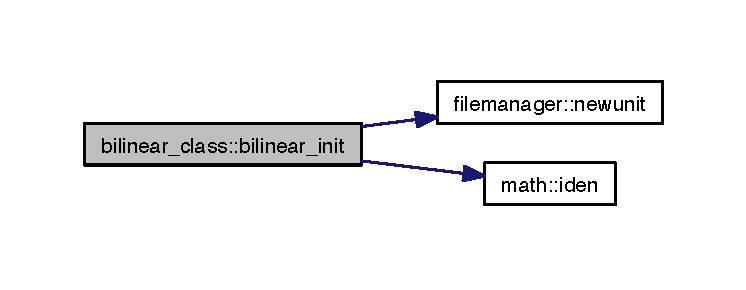
\includegraphics[width=350pt]{classbilinear__class_a767f35cd3ebd5ef00f6a55fd775c3a27_cgraph}
\end{center}
\end{figure}


\hypertarget{classbilinear__class_ae206ab58d224c9a0b7e25ac038e003ae}{\index{bilinear\-\_\-class@{bilinear\-\_\-class}!bilinear\-\_\-kill@{bilinear\-\_\-kill}}
\index{bilinear\-\_\-kill@{bilinear\-\_\-kill}!bilinear_class@{bilinear\-\_\-class}}
\subsubsection[{bilinear\-\_\-kill}]{\setlength{\rightskip}{0pt plus 5cm}subroutine bilinear\-\_\-class\-::bilinear\-\_\-kill (
\begin{DoxyParamCaption}
\item[{type({\bf bilinear}), intent(inout)}]{this}
\end{DoxyParamCaption}
)\hspace{0.3cm}{\ttfamily [private]}}}\label{classbilinear__class_ae206ab58d224c9a0b7e25ac038e003ae}


Destroys the bilinear coupling object. 


\begin{DoxyParams}{Parameters}
{\em this} & is the bilinear coupling object to be destroyed. \\
\hline
\end{DoxyParams}
\hypertarget{classbilinear__class_aac587f5ea6d66ee89ff3210b10569777}{\index{bilinear\-\_\-class@{bilinear\-\_\-class}!bilinear\-\_\-resample@{bilinear\-\_\-resample}}
\index{bilinear\-\_\-resample@{bilinear\-\_\-resample}!bilinear_class@{bilinear\-\_\-class}}
\subsubsection[{bilinear\-\_\-resample}]{\setlength{\rightskip}{0pt plus 5cm}subroutine bilinear\-\_\-class\-::bilinear\-\_\-resample (
\begin{DoxyParamCaption}
\item[{type({\bf bilinear}), intent(inout)}]{this}
\end{DoxyParamCaption}
)\hspace{0.3cm}{\ttfamily [private]}}}\label{classbilinear__class_aac587f5ea6d66ee89ff3210b10569777}


Re-\/initiallizes the bilinear coupling object. 


\begin{DoxyParams}{Parameters}
{\em this} & is the bilinear coupling object to be re-\/initialized. \\
\hline
\end{DoxyParams}


Here is the call graph for this function\-:
\nopagebreak
\begin{figure}[H]
\begin{center}
\leavevmode
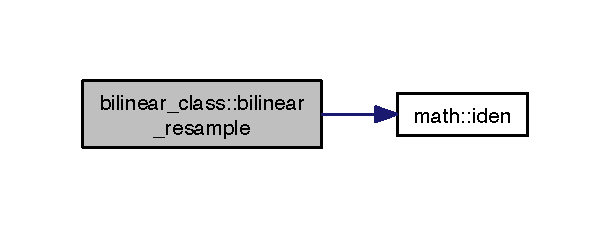
\includegraphics[width=294pt]{classbilinear__class_aac587f5ea6d66ee89ff3210b10569777_cgraph}
\end{center}
\end{figure}


\hypertarget{classbilinear__class_a5fe875f5d4db31ef7a7e721ba4a0146a}{\index{bilinear\-\_\-class@{bilinear\-\_\-class}!bilinear\-\_\-save@{bilinear\-\_\-save}}
\index{bilinear\-\_\-save@{bilinear\-\_\-save}!bilinear_class@{bilinear\-\_\-class}}
\subsubsection[{bilinear\-\_\-save}]{\setlength{\rightskip}{0pt plus 5cm}subroutine bilinear\-\_\-class\-::bilinear\-\_\-save (
\begin{DoxyParamCaption}
\item[{type({\bf bilinear}), intent(in)}]{this, }
\item[{character$\ast$($\ast$), intent(in)}]{file}
\end{DoxyParamCaption}
)\hspace{0.3cm}{\ttfamily [private]}}}\label{classbilinear__class_a5fe875f5d4db31ef7a7e721ba4a0146a}


Saves the current state of the bilinear coupling object to file. 


\begin{DoxyParams}[1]{Parameters}
\mbox{\tt in}  & {\em this} & is the bilinear coupling object to be updated. \\
\hline
\mbox{\tt in}  & {\em file} & is a string containing the location of the save file. \\
\hline
\end{DoxyParams}


Here is the call graph for this function\-:
\nopagebreak
\begin{figure}[H]
\begin{center}
\leavevmode
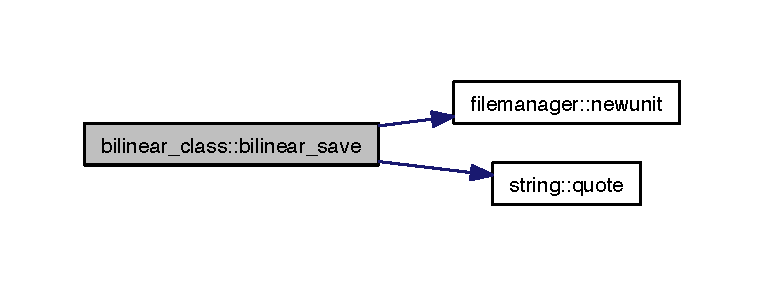
\includegraphics[width=350pt]{classbilinear__class_a5fe875f5d4db31ef7a7e721ba4a0146a_cgraph}
\end{center}
\end{figure}


\hypertarget{classbilinear__class_a37ead815723c4c247c156200f5bf4721}{\index{bilinear\-\_\-class@{bilinear\-\_\-class}!bilinear\-\_\-update@{bilinear\-\_\-update}}
\index{bilinear\-\_\-update@{bilinear\-\_\-update}!bilinear_class@{bilinear\-\_\-class}}
\subsubsection[{bilinear\-\_\-update}]{\setlength{\rightskip}{0pt plus 5cm}subroutine bilinear\-\_\-class\-::bilinear\-\_\-update (
\begin{DoxyParamCaption}
\item[{type({\bf bilinear}), intent(inout)}]{this}
\end{DoxyParamCaption}
)\hspace{0.3cm}{\ttfamily [private]}}}\label{classbilinear__class_a37ead815723c4c247c156200f5bf4721}


Computes the current state of bilinear coupling object. 


\begin{DoxyParams}{Parameters}
{\em this} & is the bilinear coupling object to be updated. \\
\hline
\end{DoxyParams}


The documentation for this module was generated from the following file\-:\begin{DoxyCompactItemize}
\item 
src/\hyperlink{bilinear_8f90}{bilinear.\-f90}\end{DoxyCompactItemize}

\hypertarget{interfacedipoles__class_1_1check}{\section{dipoles\-\_\-class\-:\-:check Interface Reference}
\label{interfacedipoles__class_1_1check}\index{dipoles\-\_\-class\-::check@{dipoles\-\_\-class\-::check}}
}
\subsection*{Private Member Functions}
\begin{DoxyCompactItemize}
\item 
integer(short) function \hyperlink{interfacedipoles__class_1_1check_a1afd058d4265177ebf90bf98c6811d09}{dipoles\-\_\-check} (this)
\end{DoxyCompactItemize}


\subsection{Member Function/\-Subroutine Documentation}
\hypertarget{interfacedipoles__class_1_1check_a1afd058d4265177ebf90bf98c6811d09}{\index{dipoles\-\_\-class\-::check@{dipoles\-\_\-class\-::check}!dipoles\-\_\-check@{dipoles\-\_\-check}}
\index{dipoles\-\_\-check@{dipoles\-\_\-check}!dipoles_class::check@{dipoles\-\_\-class\-::check}}
\subsubsection[{dipoles\-\_\-check}]{\setlength{\rightskip}{0pt plus 5cm}integer(short) function dipoles\-\_\-class\-::check\-::dipoles\-\_\-check (
\begin{DoxyParamCaption}
\item[{type({\bf dipoles}), intent(in)}]{this}
\end{DoxyParamCaption}
)\hspace{0.3cm}{\ttfamily [private]}}}\label{interfacedipoles__class_1_1check_a1afd058d4265177ebf90bf98c6811d09}


Here is the caller graph for this function\-:
\nopagebreak
\begin{figure}[H]
\begin{center}
\leavevmode
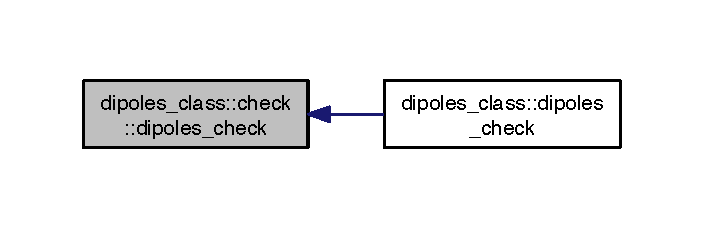
\includegraphics[width=338pt]{interfacedipoles__class_1_1check_a1afd058d4265177ebf90bf98c6811d09_icgraph}
\end{center}
\end{figure}




The documentation for this interface was generated from the following file\-:\begin{DoxyCompactItemize}
\item 
src/\hyperlink{dipoles_8f90}{dipoles.\-f90}\end{DoxyCompactItemize}

\hypertarget{interfacehs__class_1_1check}{}\section{hs\+\_\+class\+:\+:check Interface Reference}
\label{interfacehs__class_1_1check}\index{hs\+\_\+class\+::check@{hs\+\_\+class\+::check}}


Check is a function that checks if the attributes of the hs type are within acceptable values.  


\subsection*{Private Member Functions}
\begin{DoxyCompactItemize}
\item 
integer(short) function \hyperlink{interfacehs__class_1_1check_a5109e86865a66c671c91e253adea4ac1}{hs\+\_\+check} (this)
\end{DoxyCompactItemize}


\subsection{Detailed Description}
Check is a function that checks if the attributes of the hs type are within acceptable values. 

\begin{DoxyReturn}{Returns}
The integer 0 if no attribute check fails. The first failed attribute check will cause this function to return the integer 1 and issue a warning stating the failed check. This warning may cause the program to stop according to the loglevel set by the user. 
\end{DoxyReturn}


\subsection{Member Function/\+Subroutine Documentation}
\mbox{\Hypertarget{interfacehs__class_1_1check_a5109e86865a66c671c91e253adea4ac1}\label{interfacehs__class_1_1check_a5109e86865a66c671c91e253adea4ac1}} 
\index{hs\+\_\+class\+::check@{hs\+\_\+class\+::check}!hs\+\_\+check@{hs\+\_\+check}}
\index{hs\+\_\+check@{hs\+\_\+check}!hs\+\_\+class\+::check@{hs\+\_\+class\+::check}}
\subsubsection{\texorpdfstring{hs\+\_\+check()}{hs\_check()}}
{\footnotesize\ttfamily integer(short) function hs\+\_\+class\+::check\+::hs\+\_\+check (\begin{DoxyParamCaption}\item[{type(\hyperlink{strucths__class_1_1hs}{hs}), intent(in)}]{this }\end{DoxyParamCaption})\hspace{0.3cm}{\ttfamily [private]}}



The documentation for this interface was generated from the following file\+:\begin{DoxyCompactItemize}
\item 
src/\hyperlink{hs_8f90}{hs.\+f90}\end{DoxyCompactItemize}

\hypertarget{interfacebilinear__class_1_1check}{}\section{bilinear\+\_\+class\+:\+:check Interface Reference}
\label{interfacebilinear__class_1_1check}\index{bilinear\+\_\+class\+::check@{bilinear\+\_\+class\+::check}}


Checks the bilinear object.  


\subsection*{Private Member Functions}
\begin{DoxyCompactItemize}
\item 
integer(short) function \hyperlink{interfacebilinear__class_1_1check_a2f5e2ad8486524baf370c82792c889a6}{bilinear\+\_\+check} (this)
\begin{DoxyCompactList}\small\item\em Checks the bilinear coupling object. \end{DoxyCompactList}\end{DoxyCompactItemize}


\subsection{Detailed Description}
Checks the bilinear object. 

\subsection{Member Function/\+Subroutine Documentation}
\mbox{\Hypertarget{interfacebilinear__class_1_1check_a2f5e2ad8486524baf370c82792c889a6}\label{interfacebilinear__class_1_1check_a2f5e2ad8486524baf370c82792c889a6}} 
\index{bilinear\+\_\+class\+::check@{bilinear\+\_\+class\+::check}!bilinear\+\_\+check@{bilinear\+\_\+check}}
\index{bilinear\+\_\+check@{bilinear\+\_\+check}!bilinear\+\_\+class\+::check@{bilinear\+\_\+class\+::check}}
\subsubsection{\texorpdfstring{bilinear\+\_\+check()}{bilinear\_check()}}
{\footnotesize\ttfamily integer(short) function bilinear\+\_\+class\+::check\+::bilinear\+\_\+check (\begin{DoxyParamCaption}\item[{type(\hyperlink{structbilinear__class_1_1bilinear}{bilinear}), intent(in)}]{this }\end{DoxyParamCaption})\hspace{0.3cm}{\ttfamily [private]}}



Checks the bilinear coupling object. 


\begin{DoxyParams}[1]{Parameters}
\mbox{\tt in}  & {\em this} & is the bilinear coupling object to be updated. \\
\hline
\mbox{\tt in}  & {\em msg} & is an optional string message to preface the displayed object. \\
\hline
\mbox{\tt in}  & {\em file} & is an optional string containing the location of a file where the display output gets forwarded. \\
\hline
\end{DoxyParams}


The documentation for this interface was generated from the following file\+:\begin{DoxyCompactItemize}
\item 
src/\hyperlink{bilinear_8f90}{bilinear.\+f90}\end{DoxyCompactItemize}

\hypertarget{interfaceclassical__class_1_1check}{\section{classical\-\_\-class\-:\-:check Interface Reference}
\label{interfaceclassical__class_1_1check}\index{classical\-\_\-class\-::check@{classical\-\_\-class\-::check}}
}
\subsection*{Private Member Functions}
\begin{DoxyCompactItemize}
\item 
integer(short) function \hyperlink{interfaceclassical__class_1_1check_a4782f7126730047517a82ba29f0355f3}{classical\-\_\-check} (this)
\end{DoxyCompactItemize}


\subsection{Member Function/\-Subroutine Documentation}
\hypertarget{interfaceclassical__class_1_1check_a4782f7126730047517a82ba29f0355f3}{\index{classical\-\_\-class\-::check@{classical\-\_\-class\-::check}!classical\-\_\-check@{classical\-\_\-check}}
\index{classical\-\_\-check@{classical\-\_\-check}!classical_class::check@{classical\-\_\-class\-::check}}
\subsubsection[{classical\-\_\-check}]{\setlength{\rightskip}{0pt plus 5cm}integer(short) function classical\-\_\-class\-::check\-::classical\-\_\-check (
\begin{DoxyParamCaption}
\item[{type({\bf classical}), intent(in)}]{this}
\end{DoxyParamCaption}
)\hspace{0.3cm}{\ttfamily [private]}}}\label{interfaceclassical__class_1_1check_a4782f7126730047517a82ba29f0355f3}


Here is the caller graph for this function\-:
\nopagebreak
\begin{figure}[H]
\begin{center}
\leavevmode
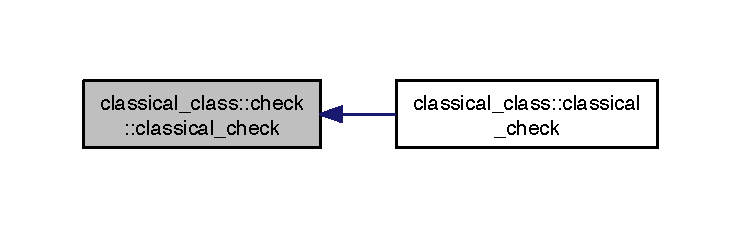
\includegraphics[width=350pt]{interfaceclassical__class_1_1check_a4782f7126730047517a82ba29f0355f3_icgraph}
\end{center}
\end{figure}




The documentation for this interface was generated from the following file\-:\begin{DoxyCompactItemize}
\item 
src/\hyperlink{classical_8f90}{classical.\-f90}\end{DoxyCompactItemize}

\hypertarget{interfaceharmonicbath__class_1_1check}{}\section{harmonicbath\+\_\+class\+:\+:check Interface Reference}
\label{interfaceharmonicbath__class_1_1check}\index{harmonicbath\+\_\+class\+::check@{harmonicbath\+\_\+class\+::check}}
\subsection*{Private Member Functions}
\begin{DoxyCompactItemize}
\item 
integer(short) function \hyperlink{interfaceharmonicbath__class_1_1check_aad3d94e95a03caa54e1ba8541130b2df}{harmonicbath\+\_\+check} (this)
\end{DoxyCompactItemize}


\subsection{Member Function/\+Subroutine Documentation}
\mbox{\Hypertarget{interfaceharmonicbath__class_1_1check_aad3d94e95a03caa54e1ba8541130b2df}\label{interfaceharmonicbath__class_1_1check_aad3d94e95a03caa54e1ba8541130b2df}} 
\index{harmonicbath\+\_\+class\+::check@{harmonicbath\+\_\+class\+::check}!harmonicbath\+\_\+check@{harmonicbath\+\_\+check}}
\index{harmonicbath\+\_\+check@{harmonicbath\+\_\+check}!harmonicbath\+\_\+class\+::check@{harmonicbath\+\_\+class\+::check}}
\subsubsection{\texorpdfstring{harmonicbath\+\_\+check()}{harmonicbath\_check()}}
{\footnotesize\ttfamily integer(short) function harmonicbath\+\_\+class\+::check\+::harmonicbath\+\_\+check (\begin{DoxyParamCaption}\item[{type(\hyperlink{structharmonicbath__class_1_1harmonicbath}{harmonicbath}), intent(in)}]{this }\end{DoxyParamCaption})\hspace{0.3cm}{\ttfamily [private]}}



The documentation for this interface was generated from the following file\+:\begin{DoxyCompactItemize}
\item 
src/\hyperlink{harmonicbath_8f90}{harmonicbath.\+f90}\end{DoxyCompactItemize}

\hypertarget{interfacepldm__class_1_1check}{}\section{pldm\+\_\+class\+:\+:check Interface Reference}
\label{interfacepldm__class_1_1check}\index{pldm\+\_\+class\+::check@{pldm\+\_\+class\+::check}}
\subsection*{Private Member Functions}
\begin{DoxyCompactItemize}
\item 
integer(short) function \hyperlink{interfacepldm__class_1_1check_a1487f82ce4231c72f10b8d47af8e798b}{pldm\+\_\+check} (this)
\end{DoxyCompactItemize}


\subsection{Member Function/\+Subroutine Documentation}
\mbox{\Hypertarget{interfacepldm__class_1_1check_a1487f82ce4231c72f10b8d47af8e798b}\label{interfacepldm__class_1_1check_a1487f82ce4231c72f10b8d47af8e798b}} 
\index{pldm\+\_\+class\+::check@{pldm\+\_\+class\+::check}!pldm\+\_\+check@{pldm\+\_\+check}}
\index{pldm\+\_\+check@{pldm\+\_\+check}!pldm\+\_\+class\+::check@{pldm\+\_\+class\+::check}}
\subsubsection{\texorpdfstring{pldm\+\_\+check()}{pldm\_check()}}
{\footnotesize\ttfamily integer(short) function pldm\+\_\+class\+::check\+::pldm\+\_\+check (\begin{DoxyParamCaption}\item[{type(\hyperlink{structpldm__class_1_1pldm}{pldm}), intent(in)}]{this }\end{DoxyParamCaption})\hspace{0.3cm}{\ttfamily [private]}}



The documentation for this interface was generated from the following file\+:\begin{DoxyCompactItemize}
\item 
src/\hyperlink{_p_l_d_m_8f90}{P\+L\+D\+M.\+f90}\end{DoxyCompactItemize}

\hypertarget{interfacehb__class_1_1check}{\section{hb\+\_\+class\+:\+:check Interface Reference}
\label{interfacehb__class_1_1check}\index{hb\+\_\+class\+::check@{hb\+\_\+class\+::check}}
}
\subsection*{Private Member Functions}
\begin{DoxyCompactItemize}
\item 
integer(short) function \hyperlink{interfacehb__class_1_1check_af3a0cc17992c073f36b86211a97625a2}{hb\+\_\+check} (this)
\item 
integer(short) function \hyperlink{interfacehb__class_1_1check_af3a0cc17992c073f36b86211a97625a2}{hb\+\_\+check} (this)
\end{DoxyCompactItemize}


\subsection{Member Function/\+Subroutine Documentation}
\hypertarget{interfacehb__class_1_1check_af3a0cc17992c073f36b86211a97625a2}{\index{hb\+\_\+class\+::check@{hb\+\_\+class\+::check}!hb\+\_\+check@{hb\+\_\+check}}
\index{hb\+\_\+check@{hb\+\_\+check}!hb\+\_\+class\+::check@{hb\+\_\+class\+::check}}
\subsubsection[{hb\+\_\+check}]{\setlength{\rightskip}{0pt plus 5cm}integer(short) function hb\+\_\+class\+::check\+::hb\+\_\+check (
\begin{DoxyParamCaption}
\item[{type({\bf hb}), intent(in)}]{this}
\end{DoxyParamCaption}
)\hspace{0.3cm}{\ttfamily [private]}}}\label{interfacehb__class_1_1check_af3a0cc17992c073f36b86211a97625a2}


Here is the caller graph for this function\+:\nopagebreak
\begin{figure}[H]
\begin{center}
\leavevmode
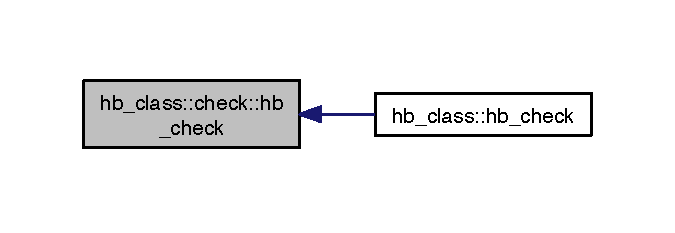
\includegraphics[width=324pt]{interfacehb__class_1_1check_af3a0cc17992c073f36b86211a97625a2_icgraph}
\end{center}
\end{figure}


\hypertarget{interfacehb__class_1_1check_af3a0cc17992c073f36b86211a97625a2}{\index{hb\+\_\+class\+::check@{hb\+\_\+class\+::check}!hb\+\_\+check@{hb\+\_\+check}}
\index{hb\+\_\+check@{hb\+\_\+check}!hb\+\_\+class\+::check@{hb\+\_\+class\+::check}}
\subsubsection[{hb\+\_\+check}]{\setlength{\rightskip}{0pt plus 5cm}integer(short) function hb\+\_\+class\+::check\+::hb\+\_\+check (
\begin{DoxyParamCaption}
\item[{type({\bf hb}), intent(in)}]{this}
\end{DoxyParamCaption}
)\hspace{0.3cm}{\ttfamily [private]}}}\label{interfacehb__class_1_1check_af3a0cc17992c073f36b86211a97625a2}


The documentation for this interface was generated from the following files\+:\begin{DoxyCompactItemize}
\item 
src/\hyperlink{hb_8f90}{hb.\+f90}\item 
src/\hyperlink{hbcopy_8f90}{hbcopy.\+f90}\end{DoxyCompactItemize}

\hypertarget{interfacequantum__class_1_1check}{}\section{quantum\+\_\+class\+:\+:check Interface Reference}
\label{interfacequantum__class_1_1check}\index{quantum\+\_\+class\+::check@{quantum\+\_\+class\+::check}}
\subsection*{Private Member Functions}
\begin{DoxyCompactItemize}
\item 
integer(short) function \hyperlink{interfacequantum__class_1_1check_a05d5b06760f2f7349f19267467e6da00}{quantum\+\_\+check} (this)
\end{DoxyCompactItemize}


\subsection{Member Function/\+Subroutine Documentation}
\mbox{\Hypertarget{interfacequantum__class_1_1check_a05d5b06760f2f7349f19267467e6da00}\label{interfacequantum__class_1_1check_a05d5b06760f2f7349f19267467e6da00}} 
\index{quantum\+\_\+class\+::check@{quantum\+\_\+class\+::check}!quantum\+\_\+check@{quantum\+\_\+check}}
\index{quantum\+\_\+check@{quantum\+\_\+check}!quantum\+\_\+class\+::check@{quantum\+\_\+class\+::check}}
\subsubsection{\texorpdfstring{quantum\+\_\+check()}{quantum\_check()}}
{\footnotesize\ttfamily integer(short) function quantum\+\_\+class\+::check\+::quantum\+\_\+check (\begin{DoxyParamCaption}\item[{type(\hyperlink{structquantum__class_1_1quantum}{quantum}), intent(in)}]{this }\end{DoxyParamCaption})\hspace{0.3cm}{\ttfamily [private]}}



The documentation for this interface was generated from the following file\+:\begin{DoxyCompactItemize}
\item 
src/\hyperlink{quantum_8f90}{quantum.\+f90}\end{DoxyCompactItemize}

\hypertarget{interfacespectrometer__class_1_1check}{}\section{spectrometer\+\_\+class\+:\+:check Interface Reference}
\label{interfacespectrometer__class_1_1check}\index{spectrometer\+\_\+class\+::check@{spectrometer\+\_\+class\+::check}}


Function that checks the spectrum type.  


\subsection*{Private Member Functions}
\begin{DoxyCompactItemize}
\item 
integer(short) function \hyperlink{interfacespectrometer__class_1_1check_a1d14d7c8751b28855644e3d7ab669260}{spectrum\+\_\+check} (this)
\begin{DoxyCompactList}\small\item\em Checks spectrum type \end{DoxyCompactList}\end{DoxyCompactItemize}


\subsection{Detailed Description}
Function that checks the spectrum type. 

\subsection{Member Function/\+Subroutine Documentation}
\mbox{\Hypertarget{interfacespectrometer__class_1_1check_a1d14d7c8751b28855644e3d7ab669260}\label{interfacespectrometer__class_1_1check_a1d14d7c8751b28855644e3d7ab669260}} 
\index{spectrometer\+\_\+class\+::check@{spectrometer\+\_\+class\+::check}!spectrum\+\_\+check@{spectrum\+\_\+check}}
\index{spectrum\+\_\+check@{spectrum\+\_\+check}!spectrometer\+\_\+class\+::check@{spectrometer\+\_\+class\+::check}}
\subsubsection{\texorpdfstring{spectrum\+\_\+check()}{spectrum\_check()}}
{\footnotesize\ttfamily integer(short) function spectrometer\+\_\+class\+::check\+::spectrum\+\_\+check (\begin{DoxyParamCaption}\item[{type(\hyperlink{structspectrometer__class_1_1spectrum}{spectrum}), intent(in)}]{this }\end{DoxyParamCaption})\hspace{0.3cm}{\ttfamily [private]}}



Checks spectrum type 



The documentation for this interface was generated from the following file\+:\begin{DoxyCompactItemize}
\item 
src/\hyperlink{spectrometer_8f90}{spectrometer.\+f90}\end{DoxyCompactItemize}

\hypertarget{interfacecoupling__class_1_1check}{\section{coupling\-\_\-class\-:\-:check Interface Reference}
\label{interfacecoupling__class_1_1check}\index{coupling\-\_\-class\-::check@{coupling\-\_\-class\-::check}}
}
\subsection*{Private Member Functions}
\begin{DoxyCompactItemize}
\item 
integer(short) function \hyperlink{interfacecoupling__class_1_1check_a79a4c19eeb3531c0379020d9dcd90247}{coupling\-\_\-check} (this)
\end{DoxyCompactItemize}


\subsection{Member Function/\-Subroutine Documentation}
\hypertarget{interfacecoupling__class_1_1check_a79a4c19eeb3531c0379020d9dcd90247}{\index{coupling\-\_\-class\-::check@{coupling\-\_\-class\-::check}!coupling\-\_\-check@{coupling\-\_\-check}}
\index{coupling\-\_\-check@{coupling\-\_\-check}!coupling_class::check@{coupling\-\_\-class\-::check}}
\subsubsection[{coupling\-\_\-check}]{\setlength{\rightskip}{0pt plus 5cm}integer(short) function coupling\-\_\-class\-::check\-::coupling\-\_\-check (
\begin{DoxyParamCaption}
\item[{type({\bf coupling}), intent(in)}]{this}
\end{DoxyParamCaption}
)\hspace{0.3cm}{\ttfamily [private]}}}\label{interfacecoupling__class_1_1check_a79a4c19eeb3531c0379020d9dcd90247}


Here is the caller graph for this function\-:
\nopagebreak
\begin{figure}[H]
\begin{center}
\leavevmode
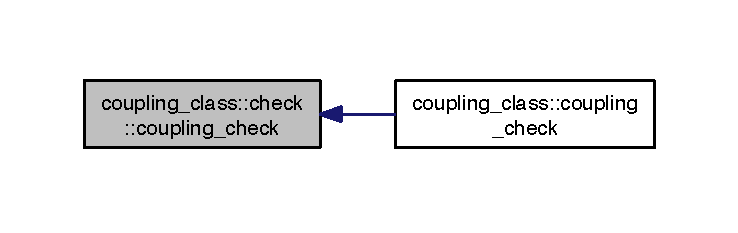
\includegraphics[width=350pt]{interfacecoupling__class_1_1check_a79a4c19eeb3531c0379020d9dcd90247_icgraph}
\end{center}
\end{figure}




The documentation for this interface was generated from the following file\-:\begin{DoxyCompactItemize}
\item 
src/\hyperlink{coupling_8f90}{coupling.\-f90}\end{DoxyCompactItemize}

\hypertarget{interfacehc__class_1_1check}{}\section{hc\+\_\+class\+:\+:check Interface Reference}
\label{interfacehc__class_1_1check}\index{hc\+\_\+class\+::check@{hc\+\_\+class\+::check}}
\subsection*{Private Member Functions}
\begin{DoxyCompactItemize}
\item 
integer(short) function \hyperlink{interfacehc__class_1_1check_a6b3cd4e85957d3b216af265404780025}{hc\+\_\+check} (this)
\end{DoxyCompactItemize}


\subsection{Member Function/\+Subroutine Documentation}
\mbox{\Hypertarget{interfacehc__class_1_1check_a6b3cd4e85957d3b216af265404780025}\label{interfacehc__class_1_1check_a6b3cd4e85957d3b216af265404780025}} 
\index{hc\+\_\+class\+::check@{hc\+\_\+class\+::check}!hc\+\_\+check@{hc\+\_\+check}}
\index{hc\+\_\+check@{hc\+\_\+check}!hc\+\_\+class\+::check@{hc\+\_\+class\+::check}}
\subsubsection{\texorpdfstring{hc\+\_\+check()}{hc\_check()}}
{\footnotesize\ttfamily integer(short) function hc\+\_\+class\+::check\+::hc\+\_\+check (\begin{DoxyParamCaption}\item[{type(\hyperlink{structhc__class_1_1hc}{hc}), intent(in)}]{this }\end{DoxyParamCaption})\hspace{0.3cm}{\ttfamily [private]}}



The documentation for this interface was generated from the following file\+:\begin{DoxyCompactItemize}
\item 
src/\hyperlink{hc_8f90}{hc.\+f90}\end{DoxyCompactItemize}

\hypertarget{interfacetemplate__class_1_1check}{}\section{template\+\_\+class\+:\+:check Interface Reference}
\label{interfacetemplate__class_1_1check}\index{template\+\_\+class\+::check@{template\+\_\+class\+::check}}


Checks that the T\+E\+M\+P\+L\+A\+TE object.  


\subsection*{Private Member Functions}
\begin{DoxyCompactItemize}
\item 
integer(short) function \hyperlink{interfacetemplate__class_1_1check_aad08be82f9ea98602fed47523c5d5fa7}{template\+\_\+check} (this)
\begin{DoxyCompactList}\small\item\em Displays the T\+E\+M\+P\+L\+A\+TE object. \end{DoxyCompactList}\end{DoxyCompactItemize}


\subsection{Detailed Description}
Checks that the T\+E\+M\+P\+L\+A\+TE object. 

\subsection{Member Function/\+Subroutine Documentation}
\mbox{\Hypertarget{interfacetemplate__class_1_1check_aad08be82f9ea98602fed47523c5d5fa7}\label{interfacetemplate__class_1_1check_aad08be82f9ea98602fed47523c5d5fa7}} 
\index{template\+\_\+class\+::check@{template\+\_\+class\+::check}!template\+\_\+check@{template\+\_\+check}}
\index{template\+\_\+check@{template\+\_\+check}!template\+\_\+class\+::check@{template\+\_\+class\+::check}}
\subsubsection{\texorpdfstring{template\+\_\+check()}{template\_check()}}
{\footnotesize\ttfamily integer(short) function template\+\_\+class\+::check\+::template\+\_\+check (\begin{DoxyParamCaption}\item[{type(\hyperlink{structtemplate__class_1_1template}{template}), intent(in)}]{this }\end{DoxyParamCaption})\hspace{0.3cm}{\ttfamily [private]}}



Displays the T\+E\+M\+P\+L\+A\+TE object. 


\begin{DoxyParams}[1]{Parameters}
\mbox{\tt in}  & {\em this} & is the T\+E\+M\+P\+L\+A\+TE object to be checked. \\
\hline
\end{DoxyParams}
\begin{DoxyReturn}{Returns}
Nothing if all checks pass or 1 and a warn for the first failed check. 
\end{DoxyReturn}
\begin{DoxyRemark}{Remarks}
Will exit after first failed check. 
\end{DoxyRemark}


The documentation for this interface was generated from the following file\+:\begin{DoxyCompactItemize}
\item 
src/\hyperlink{_t_e_m_p_l_a_t_e_8f90}{T\+E\+M\+P\+L\+A\+T\+E.\+f90}\end{DoxyCompactItemize}

\hypertarget{interfacefilemanager_1_1check}{\section{filemanager\-:\-:check Interface Reference}
\label{interfacefilemanager_1_1check}\index{filemanager\-::check@{filemanager\-::check}}
}
\subsection*{Private Member Functions}
\begin{DoxyCompactItemize}
\item 
integer(short) function \hyperlink{interfacefilemanager_1_1check_a3e31b7fed9f846da1c5ce4f52823ee88}{checkfile} (file)
\end{DoxyCompactItemize}


\subsection{Member Function/\-Subroutine Documentation}
\hypertarget{interfacefilemanager_1_1check_a3e31b7fed9f846da1c5ce4f52823ee88}{\index{filemanager\-::check@{filemanager\-::check}!checkfile@{checkfile}}
\index{checkfile@{checkfile}!filemanager::check@{filemanager\-::check}}
\subsubsection[{checkfile}]{\setlength{\rightskip}{0pt plus 5cm}integer(short) function filemanager\-::check\-::checkfile (
\begin{DoxyParamCaption}
\item[{character$\ast$($\ast$), intent(in)}]{file}
\end{DoxyParamCaption}
)\hspace{0.3cm}{\ttfamily [private]}}}\label{interfacefilemanager_1_1check_a3e31b7fed9f846da1c5ce4f52823ee88}


Here is the caller graph for this function\-:
\nopagebreak
\begin{figure}[H]
\begin{center}
\leavevmode
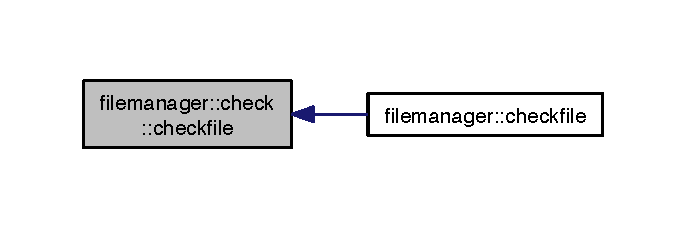
\includegraphics[width=330pt]{interfacefilemanager_1_1check_a3e31b7fed9f846da1c5ce4f52823ee88_icgraph}
\end{center}
\end{figure}




The documentation for this interface was generated from the following file\-:\begin{DoxyCompactItemize}
\item 
src/\hyperlink{utils_8f90}{utils.\-f90}\end{DoxyCompactItemize}

\hypertarget{structclassical__class_1_1classical}{\section{classical\-\_\-class\-:\-:classical Type Reference}
\label{structclassical__class_1_1classical}\index{classical\-\_\-class\-::classical@{classical\-\_\-class\-::classical}}
}
\subsection*{Private Attributes}
\begin{DoxyCompactItemize}
\item 
logical \hyperlink{structclassical__class_1_1classical_a5f61e82b2e7ad767b39cea9512cd1e79}{initialized}
\item 
\hyperlink{structclassical__class_1_1classical_a4c835c43f9359c512790ebce83387d63}{type}(hb), pointer \hyperlink{structclassical__class_1_1classical_a1b460aa0f46813107d5d6b2c6904b714}{hb}
\item 
\hyperlink{structclassical__class_1_1classical_a4c835c43f9359c512790ebce83387d63}{type}(\hyperlink{structclassical__class_1_1classical_a1b460aa0f46813107d5d6b2c6904b714}{hb}) \hyperlink{structclassical__class_1_1classical_ae02517eaafa051141de41d949d7be0ef}{primitive}
\item 
character(len=title) \hyperlink{structclassical__class_1_1classical_a4c835c43f9359c512790ebce83387d63}{type}
\item 
\hyperlink{structclassical__class_1_1classical_a4c835c43f9359c512790ebce83387d63}{type}(harmonicbath) \hyperlink{structclassical__class_1_1classical_a36ea44d91c4d0b5dd920ba9099be4ceb}{harmonicbath}
\end{DoxyCompactItemize}


\subsection{Member Data Documentation}
\hypertarget{structclassical__class_1_1classical_a36ea44d91c4d0b5dd920ba9099be4ceb}{\index{classical\-\_\-class\-::classical@{classical\-\_\-class\-::classical}!harmonicbath@{harmonicbath}}
\index{harmonicbath@{harmonicbath}!classical_class::classical@{classical\-\_\-class\-::classical}}
\subsubsection[{harmonicbath}]{\setlength{\rightskip}{0pt plus 5cm}{\bf type}(harmonicbath) classical\-\_\-class\-::classical\-::harmonicbath\hspace{0.3cm}{\ttfamily [private]}}}\label{structclassical__class_1_1classical_a36ea44d91c4d0b5dd920ba9099be4ceb}
\hypertarget{structclassical__class_1_1classical_a1b460aa0f46813107d5d6b2c6904b714}{\index{classical\-\_\-class\-::classical@{classical\-\_\-class\-::classical}!hb@{hb}}
\index{hb@{hb}!classical_class::classical@{classical\-\_\-class\-::classical}}
\subsubsection[{hb}]{\setlength{\rightskip}{0pt plus 5cm}{\bf type}(hb), pointer classical\-\_\-class\-::classical\-::hb\hspace{0.3cm}{\ttfamily [private]}}}\label{structclassical__class_1_1classical_a1b460aa0f46813107d5d6b2c6904b714}
\hypertarget{structclassical__class_1_1classical_a5f61e82b2e7ad767b39cea9512cd1e79}{\index{classical\-\_\-class\-::classical@{classical\-\_\-class\-::classical}!initialized@{initialized}}
\index{initialized@{initialized}!classical_class::classical@{classical\-\_\-class\-::classical}}
\subsubsection[{initialized}]{\setlength{\rightskip}{0pt plus 5cm}logical classical\-\_\-class\-::classical\-::initialized\hspace{0.3cm}{\ttfamily [private]}}}\label{structclassical__class_1_1classical_a5f61e82b2e7ad767b39cea9512cd1e79}
\hypertarget{structclassical__class_1_1classical_ae02517eaafa051141de41d949d7be0ef}{\index{classical\-\_\-class\-::classical@{classical\-\_\-class\-::classical}!primitive@{primitive}}
\index{primitive@{primitive}!classical_class::classical@{classical\-\_\-class\-::classical}}
\subsubsection[{primitive}]{\setlength{\rightskip}{0pt plus 5cm}{\bf type}({\bf hb}) classical\-\_\-class\-::classical\-::primitive\hspace{0.3cm}{\ttfamily [private]}}}\label{structclassical__class_1_1classical_ae02517eaafa051141de41d949d7be0ef}
\hypertarget{structclassical__class_1_1classical_a4c835c43f9359c512790ebce83387d63}{\index{classical\-\_\-class\-::classical@{classical\-\_\-class\-::classical}!type@{type}}
\index{type@{type}!classical_class::classical@{classical\-\_\-class\-::classical}}
\subsubsection[{type}]{\setlength{\rightskip}{0pt plus 5cm}character(len=title) classical\-\_\-class\-::classical\-::type\hspace{0.3cm}{\ttfamily [private]}}}\label{structclassical__class_1_1classical_a4c835c43f9359c512790ebce83387d63}


The documentation for this type was generated from the following file\-:\begin{DoxyCompactItemize}
\item 
src/\hyperlink{classical_8f90}{classical.\-f90}\end{DoxyCompactItemize}

\hypertarget{classclassical__class}{\section{classical\+\_\+class Module Reference}
\label{classclassical__class}\index{classical\+\_\+class@{classical\+\_\+class}}
}


Generic classical Class.  


\subsection*{Data Types}
\begin{DoxyCompactItemize}
\item 
interface \hyperlink{interfaceclassical__class_1_1check}{check}
\item 
type \hyperlink{structclassical__class_1_1classical}{classical}
\item 
interface \hyperlink{interfaceclassical__class_1_1display}{display}
\item 
interface \hyperlink{interfaceclassical__class_1_1kill}{kill}
\item 
interface \hyperlink{interfaceclassical__class_1_1new}{new}
\item 
interface \hyperlink{interfaceclassical__class_1_1resample}{resample}
\item 
interface \hyperlink{interfaceclassical__class_1_1save}{save}
\item 
interface \hyperlink{interfaceclassical__class_1_1update}{update}
\end{DoxyCompactItemize}
\subsection*{Private Member Functions}
\begin{DoxyCompactItemize}
\item 
subroutine \hyperlink{classclassical__class_a6e5dda0e17a3e5cb552a289231d488fd}{classical\+\_\+new} (this, type, file)
\item 
subroutine \hyperlink{classclassical__class_a88946a9bda2bac6d08860b7d96cf5219}{classical\+\_\+kill} (this)
\item 
subroutine \hyperlink{classclassical__class_afb802bbd3f8834f449275a0bdab55677}{classical\+\_\+update} (this)
\item 
subroutine \hyperlink{classclassical__class_a9b5ff74fe77b1370f4ca34d3bb3783c9}{classical\+\_\+resample} (this)
\item 
subroutine \hyperlink{classclassical__class_ac2d45f3adc9cbe9dcf22b9905ba1f649}{classical\+\_\+display} (this, msg)
\item 
subroutine \hyperlink{classclassical__class_a961b68acb4e6f345ae596a8424866657}{classical\+\_\+save} (this, file)
\item 
integer(short) function \hyperlink{classclassical__class_ab91ea3d44c25f7d544b297e0b1a4f00a}{classical\+\_\+check} (this)
\end{DoxyCompactItemize}


\subsection{Detailed Description}
Generic classical Class. 

Can assume any derived classical type \begin{DoxyAuthor}{Authors}
Daniel Montemayor 
\end{DoxyAuthor}


\subsection{Member Function/\+Subroutine Documentation}
\hypertarget{classclassical__class_ab91ea3d44c25f7d544b297e0b1a4f00a}{\index{classical\+\_\+class@{classical\+\_\+class}!classical\+\_\+check@{classical\+\_\+check}}
\index{classical\+\_\+check@{classical\+\_\+check}!classical\+\_\+class@{classical\+\_\+class}}
\subsubsection[{classical\+\_\+check}]{\setlength{\rightskip}{0pt plus 5cm}integer(short) function classical\+\_\+class\+::classical\+\_\+check (
\begin{DoxyParamCaption}
\item[{type({\bf classical}), intent(in)}]{this}
\end{DoxyParamCaption}
)\hspace{0.3cm}{\ttfamily [private]}}}\label{classclassical__class_ab91ea3d44c25f7d544b297e0b1a4f00a}
\hypertarget{classclassical__class_ac2d45f3adc9cbe9dcf22b9905ba1f649}{\index{classical\+\_\+class@{classical\+\_\+class}!classical\+\_\+display@{classical\+\_\+display}}
\index{classical\+\_\+display@{classical\+\_\+display}!classical\+\_\+class@{classical\+\_\+class}}
\subsubsection[{classical\+\_\+display}]{\setlength{\rightskip}{0pt plus 5cm}subroutine classical\+\_\+class\+::classical\+\_\+display (
\begin{DoxyParamCaption}
\item[{type({\bf classical}), intent(in)}]{this, }
\item[{character$\ast$($\ast$), intent(in), optional}]{msg}
\end{DoxyParamCaption}
)\hspace{0.3cm}{\ttfamily [private]}}}\label{classclassical__class_ac2d45f3adc9cbe9dcf22b9905ba1f649}
\hypertarget{classclassical__class_a88946a9bda2bac6d08860b7d96cf5219}{\index{classical\+\_\+class@{classical\+\_\+class}!classical\+\_\+kill@{classical\+\_\+kill}}
\index{classical\+\_\+kill@{classical\+\_\+kill}!classical\+\_\+class@{classical\+\_\+class}}
\subsubsection[{classical\+\_\+kill}]{\setlength{\rightskip}{0pt plus 5cm}subroutine classical\+\_\+class\+::classical\+\_\+kill (
\begin{DoxyParamCaption}
\item[{type({\bf classical}), intent(inout)}]{this}
\end{DoxyParamCaption}
)\hspace{0.3cm}{\ttfamily [private]}}}\label{classclassical__class_a88946a9bda2bac6d08860b7d96cf5219}
\hypertarget{classclassical__class_a6e5dda0e17a3e5cb552a289231d488fd}{\index{classical\+\_\+class@{classical\+\_\+class}!classical\+\_\+new@{classical\+\_\+new}}
\index{classical\+\_\+new@{classical\+\_\+new}!classical\+\_\+class@{classical\+\_\+class}}
\subsubsection[{classical\+\_\+new}]{\setlength{\rightskip}{0pt plus 5cm}subroutine classical\+\_\+class\+::classical\+\_\+new (
\begin{DoxyParamCaption}
\item[{type({\bf classical}), intent(inout), target}]{this, }
\item[{character$\ast$($\ast$), intent(in), optional}]{type, }
\item[{character$\ast$($\ast$), intent(in), optional}]{file}
\end{DoxyParamCaption}
)\hspace{0.3cm}{\ttfamily [private]}}}\label{classclassical__class_a6e5dda0e17a3e5cb552a289231d488fd}


Here is the call graph for this function\+:\nopagebreak
\begin{figure}[H]
\begin{center}
\leavevmode
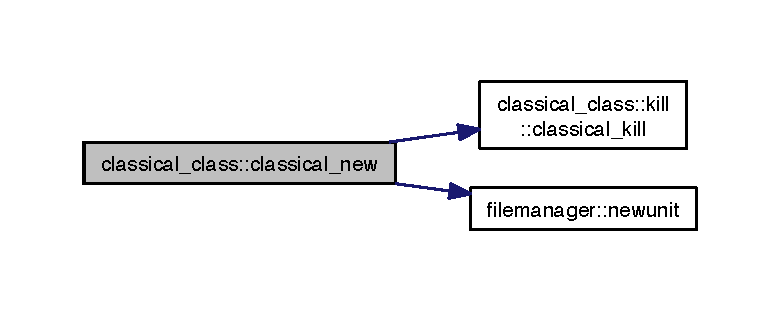
\includegraphics[width=350pt]{classclassical__class_a6e5dda0e17a3e5cb552a289231d488fd_cgraph}
\end{center}
\end{figure}


\hypertarget{classclassical__class_a9b5ff74fe77b1370f4ca34d3bb3783c9}{\index{classical\+\_\+class@{classical\+\_\+class}!classical\+\_\+resample@{classical\+\_\+resample}}
\index{classical\+\_\+resample@{classical\+\_\+resample}!classical\+\_\+class@{classical\+\_\+class}}
\subsubsection[{classical\+\_\+resample}]{\setlength{\rightskip}{0pt plus 5cm}subroutine classical\+\_\+class\+::classical\+\_\+resample (
\begin{DoxyParamCaption}
\item[{type({\bf classical}), intent(inout)}]{this}
\end{DoxyParamCaption}
)\hspace{0.3cm}{\ttfamily [private]}}}\label{classclassical__class_a9b5ff74fe77b1370f4ca34d3bb3783c9}
\hypertarget{classclassical__class_a961b68acb4e6f345ae596a8424866657}{\index{classical\+\_\+class@{classical\+\_\+class}!classical\+\_\+save@{classical\+\_\+save}}
\index{classical\+\_\+save@{classical\+\_\+save}!classical\+\_\+class@{classical\+\_\+class}}
\subsubsection[{classical\+\_\+save}]{\setlength{\rightskip}{0pt plus 5cm}subroutine classical\+\_\+class\+::classical\+\_\+save (
\begin{DoxyParamCaption}
\item[{type({\bf classical}), intent(in)}]{this, }
\item[{character$\ast$($\ast$), intent(in)}]{file}
\end{DoxyParamCaption}
)\hspace{0.3cm}{\ttfamily [private]}}}\label{classclassical__class_a961b68acb4e6f345ae596a8424866657}


Here is the call graph for this function\+:\nopagebreak
\begin{figure}[H]
\begin{center}
\leavevmode
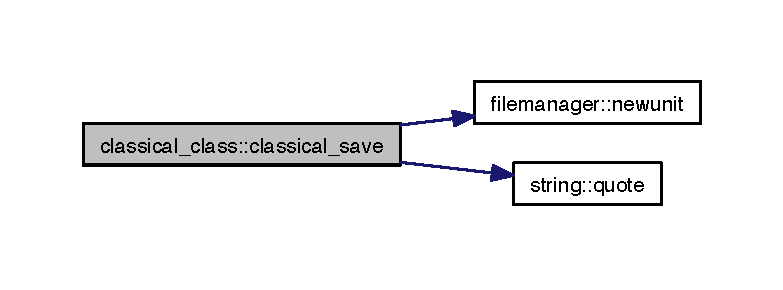
\includegraphics[width=350pt]{classclassical__class_a961b68acb4e6f345ae596a8424866657_cgraph}
\end{center}
\end{figure}


\hypertarget{classclassical__class_afb802bbd3f8834f449275a0bdab55677}{\index{classical\+\_\+class@{classical\+\_\+class}!classical\+\_\+update@{classical\+\_\+update}}
\index{classical\+\_\+update@{classical\+\_\+update}!classical\+\_\+class@{classical\+\_\+class}}
\subsubsection[{classical\+\_\+update}]{\setlength{\rightskip}{0pt plus 5cm}subroutine classical\+\_\+class\+::classical\+\_\+update (
\begin{DoxyParamCaption}
\item[{type({\bf classical}), intent(inout)}]{this}
\end{DoxyParamCaption}
)\hspace{0.3cm}{\ttfamily [private]}}}\label{classclassical__class_afb802bbd3f8834f449275a0bdab55677}


The documentation for this module was generated from the following file\+:\begin{DoxyCompactItemize}
\item 
src/\hyperlink{classical_8f90}{classical.\+f90}\end{DoxyCompactItemize}

\hypertarget{structcoupling__class_1_1coupling}{\section{coupling\-\_\-class\-:\-:coupling Type Reference}
\label{structcoupling__class_1_1coupling}\index{coupling\-\_\-class\-::coupling@{coupling\-\_\-class\-::coupling}}
}
\subsection*{Private Attributes}
\begin{DoxyCompactItemize}
\item 
logical \hyperlink{structcoupling__class_1_1coupling_affedc100d4678792285e848dd4deb313}{initialized}
\item 
\hyperlink{structcoupling__class_1_1coupling_a74b13fd447f07c24380e3913fd06d545}{type}(hc), pointer \hyperlink{structcoupling__class_1_1coupling_a2592edb5bbaf558a6196d78782c17ac2}{hc}
\item 
\hyperlink{structcoupling__class_1_1coupling_a74b13fd447f07c24380e3913fd06d545}{type}(\hyperlink{structcoupling__class_1_1coupling_a2592edb5bbaf558a6196d78782c17ac2}{hc}) \hyperlink{structcoupling__class_1_1coupling_a330aec84b5697ea890627c9a10562fb5}{primitive}
\item 
character(len=title) \hyperlink{structcoupling__class_1_1coupling_a74b13fd447f07c24380e3913fd06d545}{type}
\item 
\hyperlink{structcoupling__class_1_1coupling_a74b13fd447f07c24380e3913fd06d545}{type}(bilinear) \hyperlink{structcoupling__class_1_1coupling_a64232ba94787370a17c636014e966d13}{bilinear}
\end{DoxyCompactItemize}


\subsection{Member Data Documentation}
\hypertarget{structcoupling__class_1_1coupling_a64232ba94787370a17c636014e966d13}{\index{coupling\-\_\-class\-::coupling@{coupling\-\_\-class\-::coupling}!bilinear@{bilinear}}
\index{bilinear@{bilinear}!coupling_class::coupling@{coupling\-\_\-class\-::coupling}}
\subsubsection[{bilinear}]{\setlength{\rightskip}{0pt plus 5cm}{\bf type}(bilinear) coupling\-\_\-class\-::coupling\-::bilinear\hspace{0.3cm}{\ttfamily [private]}}}\label{structcoupling__class_1_1coupling_a64232ba94787370a17c636014e966d13}
\hypertarget{structcoupling__class_1_1coupling_a2592edb5bbaf558a6196d78782c17ac2}{\index{coupling\-\_\-class\-::coupling@{coupling\-\_\-class\-::coupling}!hc@{hc}}
\index{hc@{hc}!coupling_class::coupling@{coupling\-\_\-class\-::coupling}}
\subsubsection[{hc}]{\setlength{\rightskip}{0pt plus 5cm}{\bf type}(hc), pointer coupling\-\_\-class\-::coupling\-::hc\hspace{0.3cm}{\ttfamily [private]}}}\label{structcoupling__class_1_1coupling_a2592edb5bbaf558a6196d78782c17ac2}
\hypertarget{structcoupling__class_1_1coupling_affedc100d4678792285e848dd4deb313}{\index{coupling\-\_\-class\-::coupling@{coupling\-\_\-class\-::coupling}!initialized@{initialized}}
\index{initialized@{initialized}!coupling_class::coupling@{coupling\-\_\-class\-::coupling}}
\subsubsection[{initialized}]{\setlength{\rightskip}{0pt plus 5cm}logical coupling\-\_\-class\-::coupling\-::initialized\hspace{0.3cm}{\ttfamily [private]}}}\label{structcoupling__class_1_1coupling_affedc100d4678792285e848dd4deb313}
\hypertarget{structcoupling__class_1_1coupling_a330aec84b5697ea890627c9a10562fb5}{\index{coupling\-\_\-class\-::coupling@{coupling\-\_\-class\-::coupling}!primitive@{primitive}}
\index{primitive@{primitive}!coupling_class::coupling@{coupling\-\_\-class\-::coupling}}
\subsubsection[{primitive}]{\setlength{\rightskip}{0pt plus 5cm}{\bf type}({\bf hc}) coupling\-\_\-class\-::coupling\-::primitive\hspace{0.3cm}{\ttfamily [private]}}}\label{structcoupling__class_1_1coupling_a330aec84b5697ea890627c9a10562fb5}
\hypertarget{structcoupling__class_1_1coupling_a74b13fd447f07c24380e3913fd06d545}{\index{coupling\-\_\-class\-::coupling@{coupling\-\_\-class\-::coupling}!type@{type}}
\index{type@{type}!coupling_class::coupling@{coupling\-\_\-class\-::coupling}}
\subsubsection[{type}]{\setlength{\rightskip}{0pt plus 5cm}character(len=title) coupling\-\_\-class\-::coupling\-::type\hspace{0.3cm}{\ttfamily [private]}}}\label{structcoupling__class_1_1coupling_a74b13fd447f07c24380e3913fd06d545}


The documentation for this type was generated from the following file\-:\begin{DoxyCompactItemize}
\item 
src/\hyperlink{coupling_8f90}{coupling.\-f90}\end{DoxyCompactItemize}

\hypertarget{classcoupling__class}{\section{coupling\+\_\+class Module Reference}
\label{classcoupling__class}\index{coupling\+\_\+class@{coupling\+\_\+class}}
}


Generic coupling Class.  


\subsection*{Data Types}
\begin{DoxyCompactItemize}
\item 
interface \hyperlink{interfacecoupling__class_1_1check}{check}
\item 
type \hyperlink{structcoupling__class_1_1coupling}{coupling}
\item 
interface \hyperlink{interfacecoupling__class_1_1display}{display}
\item 
interface \hyperlink{interfacecoupling__class_1_1kill}{kill}
\item 
interface \hyperlink{interfacecoupling__class_1_1new}{new}
\item 
interface \hyperlink{interfacecoupling__class_1_1resample}{resample}
\item 
interface \hyperlink{interfacecoupling__class_1_1save}{save}
\item 
interface \hyperlink{interfacecoupling__class_1_1update}{update}
\end{DoxyCompactItemize}
\subsection*{Private Member Functions}
\begin{DoxyCompactItemize}
\item 
subroutine \hyperlink{classcoupling__class_a5fa07e475bf96111bc76820037fc26a4}{coupling\+\_\+new} (this, qs, cs, type, file)
\item 
subroutine \hyperlink{classcoupling__class_a774339d5b87453601c0664a199df7823}{coupling\+\_\+kill} (this)
\item 
subroutine \hyperlink{classcoupling__class_a034f9e137631afdb03a75cc32bf1956d}{coupling\+\_\+update} (this)
\item 
subroutine \hyperlink{classcoupling__class_ad26da11333ea64f68c25250a35287a51}{coupling\+\_\+resample} (this)
\item 
subroutine \hyperlink{classcoupling__class_a543d9a76307b2c60048d8f390fb40859}{coupling\+\_\+display} (this, msg)
\item 
subroutine \hyperlink{classcoupling__class_af46ffcc2d49425d21e248f173b5377bd}{coupling\+\_\+save} (this, file)
\item 
integer(short) function \hyperlink{classcoupling__class_a41b687a0ad543c445aa29923c229e39d}{coupling\+\_\+check} (this)
\end{DoxyCompactItemize}


\subsection{Detailed Description}
Generic coupling Class. 

Can assume any derived coupling type \begin{DoxyAuthor}{Authors}
Daniel Montemayor 
\end{DoxyAuthor}


\subsection{Member Function/\+Subroutine Documentation}
\hypertarget{classcoupling__class_a41b687a0ad543c445aa29923c229e39d}{\index{coupling\+\_\+class@{coupling\+\_\+class}!coupling\+\_\+check@{coupling\+\_\+check}}
\index{coupling\+\_\+check@{coupling\+\_\+check}!coupling\+\_\+class@{coupling\+\_\+class}}
\subsubsection[{coupling\+\_\+check}]{\setlength{\rightskip}{0pt plus 5cm}integer(short) function coupling\+\_\+class\+::coupling\+\_\+check (
\begin{DoxyParamCaption}
\item[{type({\bf coupling}), intent(in)}]{this}
\end{DoxyParamCaption}
)\hspace{0.3cm}{\ttfamily [private]}}}\label{classcoupling__class_a41b687a0ad543c445aa29923c229e39d}
\hypertarget{classcoupling__class_a543d9a76307b2c60048d8f390fb40859}{\index{coupling\+\_\+class@{coupling\+\_\+class}!coupling\+\_\+display@{coupling\+\_\+display}}
\index{coupling\+\_\+display@{coupling\+\_\+display}!coupling\+\_\+class@{coupling\+\_\+class}}
\subsubsection[{coupling\+\_\+display}]{\setlength{\rightskip}{0pt plus 5cm}subroutine coupling\+\_\+class\+::coupling\+\_\+display (
\begin{DoxyParamCaption}
\item[{type({\bf coupling}), intent(in)}]{this, }
\item[{character$\ast$($\ast$), intent(in), optional}]{msg}
\end{DoxyParamCaption}
)\hspace{0.3cm}{\ttfamily [private]}}}\label{classcoupling__class_a543d9a76307b2c60048d8f390fb40859}
\hypertarget{classcoupling__class_a774339d5b87453601c0664a199df7823}{\index{coupling\+\_\+class@{coupling\+\_\+class}!coupling\+\_\+kill@{coupling\+\_\+kill}}
\index{coupling\+\_\+kill@{coupling\+\_\+kill}!coupling\+\_\+class@{coupling\+\_\+class}}
\subsubsection[{coupling\+\_\+kill}]{\setlength{\rightskip}{0pt plus 5cm}subroutine coupling\+\_\+class\+::coupling\+\_\+kill (
\begin{DoxyParamCaption}
\item[{type({\bf coupling}), intent(inout)}]{this}
\end{DoxyParamCaption}
)\hspace{0.3cm}{\ttfamily [private]}}}\label{classcoupling__class_a774339d5b87453601c0664a199df7823}
\hypertarget{classcoupling__class_a5fa07e475bf96111bc76820037fc26a4}{\index{coupling\+\_\+class@{coupling\+\_\+class}!coupling\+\_\+new@{coupling\+\_\+new}}
\index{coupling\+\_\+new@{coupling\+\_\+new}!coupling\+\_\+class@{coupling\+\_\+class}}
\subsubsection[{coupling\+\_\+new}]{\setlength{\rightskip}{0pt plus 5cm}subroutine coupling\+\_\+class\+::coupling\+\_\+new (
\begin{DoxyParamCaption}
\item[{type({\bf coupling}), intent(inout), target}]{this, }
\item[{type(quantum), intent(inout), target}]{qs, }
\item[{type(classical), intent(inout), target}]{cs, }
\item[{character$\ast$($\ast$), intent(in), optional}]{type, }
\item[{character$\ast$($\ast$), intent(in), optional}]{file}
\end{DoxyParamCaption}
)\hspace{0.3cm}{\ttfamily [private]}}}\label{classcoupling__class_a5fa07e475bf96111bc76820037fc26a4}


Here is the call graph for this function\+:\nopagebreak
\begin{figure}[H]
\begin{center}
\leavevmode
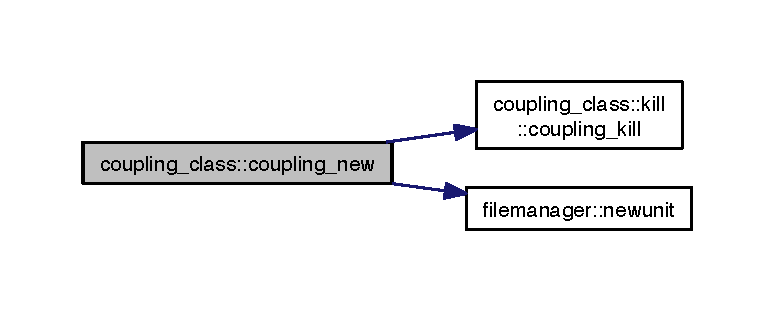
\includegraphics[width=350pt]{classcoupling__class_a5fa07e475bf96111bc76820037fc26a4_cgraph}
\end{center}
\end{figure}


\hypertarget{classcoupling__class_ad26da11333ea64f68c25250a35287a51}{\index{coupling\+\_\+class@{coupling\+\_\+class}!coupling\+\_\+resample@{coupling\+\_\+resample}}
\index{coupling\+\_\+resample@{coupling\+\_\+resample}!coupling\+\_\+class@{coupling\+\_\+class}}
\subsubsection[{coupling\+\_\+resample}]{\setlength{\rightskip}{0pt plus 5cm}subroutine coupling\+\_\+class\+::coupling\+\_\+resample (
\begin{DoxyParamCaption}
\item[{type({\bf coupling}), intent(inout)}]{this}
\end{DoxyParamCaption}
)\hspace{0.3cm}{\ttfamily [private]}}}\label{classcoupling__class_ad26da11333ea64f68c25250a35287a51}
\hypertarget{classcoupling__class_af46ffcc2d49425d21e248f173b5377bd}{\index{coupling\+\_\+class@{coupling\+\_\+class}!coupling\+\_\+save@{coupling\+\_\+save}}
\index{coupling\+\_\+save@{coupling\+\_\+save}!coupling\+\_\+class@{coupling\+\_\+class}}
\subsubsection[{coupling\+\_\+save}]{\setlength{\rightskip}{0pt plus 5cm}subroutine coupling\+\_\+class\+::coupling\+\_\+save (
\begin{DoxyParamCaption}
\item[{type({\bf coupling}), intent(in)}]{this, }
\item[{character$\ast$($\ast$), intent(in)}]{file}
\end{DoxyParamCaption}
)\hspace{0.3cm}{\ttfamily [private]}}}\label{classcoupling__class_af46ffcc2d49425d21e248f173b5377bd}


Here is the call graph for this function\+:\nopagebreak
\begin{figure}[H]
\begin{center}
\leavevmode
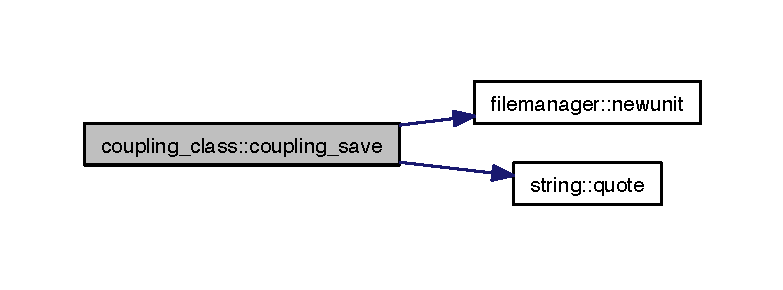
\includegraphics[width=350pt]{classcoupling__class_af46ffcc2d49425d21e248f173b5377bd_cgraph}
\end{center}
\end{figure}


\hypertarget{classcoupling__class_a034f9e137631afdb03a75cc32bf1956d}{\index{coupling\+\_\+class@{coupling\+\_\+class}!coupling\+\_\+update@{coupling\+\_\+update}}
\index{coupling\+\_\+update@{coupling\+\_\+update}!coupling\+\_\+class@{coupling\+\_\+class}}
\subsubsection[{coupling\+\_\+update}]{\setlength{\rightskip}{0pt plus 5cm}subroutine coupling\+\_\+class\+::coupling\+\_\+update (
\begin{DoxyParamCaption}
\item[{type({\bf coupling}), intent(inout)}]{this}
\end{DoxyParamCaption}
)\hspace{0.3cm}{\ttfamily [private]}}}\label{classcoupling__class_a034f9e137631afdb03a75cc32bf1956d}


The documentation for this module was generated from the following file\+:\begin{DoxyCompactItemize}
\item 
src/\hyperlink{coupling_8f90}{coupling.\+f90}\end{DoxyCompactItemize}

\hypertarget{structmolreader_1_1cryst1}{\section{molreader\+:\+:cryst1 Type Reference}
\label{structmolreader_1_1cryst1}\index{molreader\+::cryst1@{molreader\+::cryst1}}
}
\subsection*{Private Attributes}
\begin{DoxyCompactItemize}
\item 
character(len=30) \hyperlink{structmolreader_1_1cryst1_ab6ab864b10676c184026f298e2298135}{fmt}
\item 
character(len=\hyperlink{classmolreader_a8f12be3272b946fd698c9fbaf2ba9d32}{reclen}) \hyperlink{structmolreader_1_1cryst1_ae85e046760ae97562351b100fd2c9034}{recname}
\item 
real(double) \hyperlink{structmolreader_1_1cryst1_a85327bed083d1034112fc1bc78efd7e0}{a}
\item 
real(double) \hyperlink{structmolreader_1_1cryst1_a0cedac0856256f960f563ea0e3d57945}{b}
\item 
real(double) \hyperlink{structmolreader_1_1cryst1_a6269ff5021092d6d0b0185cda1572489}{c}
\item 
real(double) \hyperlink{structmolreader_1_1cryst1_a6186be5cb316849fcb7cfca0ec9c6358}{alpha}
\item 
real(double) \hyperlink{structmolreader_1_1cryst1_a0c69e8f33d0711ee345d6bfc3212e671}{beta}
\item 
real(double) \hyperlink{structmolreader_1_1cryst1_a5830f0c34f6ad1c07482a203f7a7b175}{gamma}
\item 
character(len=11) \hyperlink{structmolreader_1_1cryst1_a689985667a15167b26dee5b87a240333}{sgroup}
\item 
integer(long) \hyperlink{structmolreader_1_1cryst1_ae973dda59fd038efc49c8a247e3e71c9}{z}
\end{DoxyCompactItemize}


\subsection{Member Data Documentation}
\hypertarget{structmolreader_1_1cryst1_a85327bed083d1034112fc1bc78efd7e0}{\index{molreader\+::cryst1@{molreader\+::cryst1}!a@{a}}
\index{a@{a}!molreader\+::cryst1@{molreader\+::cryst1}}
\subsubsection[{a}]{\setlength{\rightskip}{0pt plus 5cm}real(double) molreader\+::cryst1\+::a\hspace{0.3cm}{\ttfamily [private]}}}\label{structmolreader_1_1cryst1_a85327bed083d1034112fc1bc78efd7e0}
\hypertarget{structmolreader_1_1cryst1_a6186be5cb316849fcb7cfca0ec9c6358}{\index{molreader\+::cryst1@{molreader\+::cryst1}!alpha@{alpha}}
\index{alpha@{alpha}!molreader\+::cryst1@{molreader\+::cryst1}}
\subsubsection[{alpha}]{\setlength{\rightskip}{0pt plus 5cm}real(double) molreader\+::cryst1\+::alpha\hspace{0.3cm}{\ttfamily [private]}}}\label{structmolreader_1_1cryst1_a6186be5cb316849fcb7cfca0ec9c6358}
\hypertarget{structmolreader_1_1cryst1_a0cedac0856256f960f563ea0e3d57945}{\index{molreader\+::cryst1@{molreader\+::cryst1}!b@{b}}
\index{b@{b}!molreader\+::cryst1@{molreader\+::cryst1}}
\subsubsection[{b}]{\setlength{\rightskip}{0pt plus 5cm}real(double) molreader\+::cryst1\+::b\hspace{0.3cm}{\ttfamily [private]}}}\label{structmolreader_1_1cryst1_a0cedac0856256f960f563ea0e3d57945}
\hypertarget{structmolreader_1_1cryst1_a0c69e8f33d0711ee345d6bfc3212e671}{\index{molreader\+::cryst1@{molreader\+::cryst1}!beta@{beta}}
\index{beta@{beta}!molreader\+::cryst1@{molreader\+::cryst1}}
\subsubsection[{beta}]{\setlength{\rightskip}{0pt plus 5cm}real(double) molreader\+::cryst1\+::beta\hspace{0.3cm}{\ttfamily [private]}}}\label{structmolreader_1_1cryst1_a0c69e8f33d0711ee345d6bfc3212e671}
\hypertarget{structmolreader_1_1cryst1_a6269ff5021092d6d0b0185cda1572489}{\index{molreader\+::cryst1@{molreader\+::cryst1}!c@{c}}
\index{c@{c}!molreader\+::cryst1@{molreader\+::cryst1}}
\subsubsection[{c}]{\setlength{\rightskip}{0pt plus 5cm}real(double) molreader\+::cryst1\+::c\hspace{0.3cm}{\ttfamily [private]}}}\label{structmolreader_1_1cryst1_a6269ff5021092d6d0b0185cda1572489}
\hypertarget{structmolreader_1_1cryst1_ab6ab864b10676c184026f298e2298135}{\index{molreader\+::cryst1@{molreader\+::cryst1}!fmt@{fmt}}
\index{fmt@{fmt}!molreader\+::cryst1@{molreader\+::cryst1}}
\subsubsection[{fmt}]{\setlength{\rightskip}{0pt plus 5cm}character(len=30) molreader\+::cryst1\+::fmt\hspace{0.3cm}{\ttfamily [private]}}}\label{structmolreader_1_1cryst1_ab6ab864b10676c184026f298e2298135}
\hypertarget{structmolreader_1_1cryst1_a5830f0c34f6ad1c07482a203f7a7b175}{\index{molreader\+::cryst1@{molreader\+::cryst1}!gamma@{gamma}}
\index{gamma@{gamma}!molreader\+::cryst1@{molreader\+::cryst1}}
\subsubsection[{gamma}]{\setlength{\rightskip}{0pt plus 5cm}real(double) molreader\+::cryst1\+::gamma\hspace{0.3cm}{\ttfamily [private]}}}\label{structmolreader_1_1cryst1_a5830f0c34f6ad1c07482a203f7a7b175}
\hypertarget{structmolreader_1_1cryst1_ae85e046760ae97562351b100fd2c9034}{\index{molreader\+::cryst1@{molreader\+::cryst1}!recname@{recname}}
\index{recname@{recname}!molreader\+::cryst1@{molreader\+::cryst1}}
\subsubsection[{recname}]{\setlength{\rightskip}{0pt plus 5cm}character(len={\bf reclen}) molreader\+::cryst1\+::recname\hspace{0.3cm}{\ttfamily [private]}}}\label{structmolreader_1_1cryst1_ae85e046760ae97562351b100fd2c9034}
\hypertarget{structmolreader_1_1cryst1_a689985667a15167b26dee5b87a240333}{\index{molreader\+::cryst1@{molreader\+::cryst1}!sgroup@{sgroup}}
\index{sgroup@{sgroup}!molreader\+::cryst1@{molreader\+::cryst1}}
\subsubsection[{sgroup}]{\setlength{\rightskip}{0pt plus 5cm}character(len=11) molreader\+::cryst1\+::sgroup\hspace{0.3cm}{\ttfamily [private]}}}\label{structmolreader_1_1cryst1_a689985667a15167b26dee5b87a240333}
\hypertarget{structmolreader_1_1cryst1_ae973dda59fd038efc49c8a247e3e71c9}{\index{molreader\+::cryst1@{molreader\+::cryst1}!z@{z}}
\index{z@{z}!molreader\+::cryst1@{molreader\+::cryst1}}
\subsubsection[{z}]{\setlength{\rightskip}{0pt plus 5cm}integer(long) molreader\+::cryst1\+::z\hspace{0.3cm}{\ttfamily [private]}}}\label{structmolreader_1_1cryst1_ae973dda59fd038efc49c8a247e3e71c9}


The documentation for this type was generated from the following file\+:\begin{DoxyCompactItemize}
\item 
src/\hyperlink{molreader_8f90}{molreader.\+f90}\end{DoxyCompactItemize}

\hypertarget{structdipoles__class_1_1dipoles}{\section{dipoles\+\_\+class\+:\+:dipoles Type Reference}
\label{structdipoles__class_1_1dipoles}\index{dipoles\+\_\+class\+::dipoles@{dipoles\+\_\+class\+::dipoles}}
}


derived quantum subsystem object  


\subsection*{Private Attributes}
\begin{DoxyCompactItemize}
\item 
logical \hyperlink{structdipoles__class_1_1dipoles_a62234fd4a1f98f377becc909912c8785}{initialized}
\item 
type(hs) \hyperlink{structdipoles__class_1_1dipoles_afa2264f1ca48581328e2ab0e1745db4a}{hs}
\item 
type(\hyperlink{structdipoles__class_1_1dipoles_afa2264f1ca48581328e2ab0e1745db4a}{hs}) \hyperlink{structdipoles__class_1_1dipoles_a7b6d2a8feca2c1198896fb10627d029b}{quantum}
\item 
type(\hyperlink{structdipoles__class_1_1dipoles_afa2264f1ca48581328e2ab0e1745db4a}{hs}) \hyperlink{structdipoles__class_1_1dipoles_a56b509ba86b8121570bd7a051cc77fd9}{primitive}
\item 
type(\hyperlink{structdipoles__class_1_1dipoles_afa2264f1ca48581328e2ab0e1745db4a}{hs}) \hyperlink{structdipoles__class_1_1dipoles_a2c208f78e585ed71764e1b37c20be201}{hs0}
\item 
type(\hyperlink{structdipoles__class_1_1dipoles_afa2264f1ca48581328e2ab0e1745db4a}{hs}), dimension(\+:,\+:), pointer \hyperlink{structdipoles__class_1_1dipoles_a8baa5323891d02dede517c209f432c27}{disorder}
\item 
type(\hyperlink{structdipoles__class_1_1dipoles_afa2264f1ca48581328e2ab0e1745db4a}{hs}) \hyperlink{structdipoles__class_1_1dipoles_a0d7a80c3e1a97942236e3e7a1a373cca}{less}
\item 
integer(short) \hyperlink{structdipoles__class_1_1dipoles_a1b540b65199b326d6d477307d646fb1b}{ndim}
\item 
integer(short) \hyperlink{structdipoles__class_1_1dipoles_ae809ff43be02c6f93cd5a6010368a246}{dimensionality}
\item 
integer(short), dimension(\+:,\+:), \\*
pointer \hyperlink{structdipoles__class_1_1dipoles_ae6c47d2cab7825bb83f85b624a3acb17}{of}
\item 
integer(short), dimension(\+:,\+:), \\*
pointer \hyperlink{structdipoles__class_1_1dipoles_a0b9e590823522c87bb16a014777bc66e}{transition}
\item 
integer(short) \hyperlink{structdipoles__class_1_1dipoles_a2e2a7912feab61f030584442c17fd64b}{dipoles}
\item 
integer(short) \hyperlink{structdipoles__class_1_1dipoles_a7009b45719053d38b8b082f1505127cd}{and}
\item 
integer(short), dimension(\+:,\+:), \\*
pointer \hyperlink{structdipoles__class_1_1dipoles_ae35c528d0361b9cd3c1825567339acff}{site}
\item 
integer(short), dimension(\+:,\+:), \\*
pointer \hyperlink{structdipoles__class_1_1dipoles_a959e48d8726c84ad96695f27f5a324df}{center}
\item 
integer(short), dimension(\+:,\+:), \\*
pointer \hyperlink{structdipoles__class_1_1dipoles_a30387a2e38cdc8fac3440fb019fa39e4}{mass}
\item 
real(double), dimension(\+:,\+:), \\*
pointer \hyperlink{structdipoles__class_1_1dipoles_a669f75c4c95efa1ea721ba8aa7f785d3}{dielectric}
\item 
real(double), dimension(\+:,\+:), \\*
pointer \hyperlink{structdipoles__class_1_1dipoles_a195b04ed4976581c965eb24b155dee4b}{site}
\item 
real(double), dimension(\+:,\+:), \\*
pointer \hyperlink{structdipoles__class_1_1dipoles_aa236248648a049967f193ec7a2e721a3}{to}
\item 
real(double), dimension(\+:,\+:), \\*
pointer \hyperlink{structdipoles__class_1_1dipoles_a7a0b0cffbbb4e48c4bced86e3684ac14}{optical}
\item 
real(double), dimension(\+:,\+:), \\*
pointer \hyperlink{structdipoles__class_1_1dipoles_a353f22dda5068231a14e388b11f2c5cc}{screening}
\item 
real(double) \hyperlink{structdipoles__class_1_1dipoles_a6723a79a10a1b02fe363c2fdf8d0b1aa}{gvar}
\item 
real(double) \hyperlink{structdipoles__class_1_1dipoles_a0ad3fc4bf8e3d48aea2e39d709e5f4ca}{groundstate}
\item 
real(double) \hyperlink{structdipoles__class_1_1dipoles_ac0229d4af6218531a78c4890b752a1e7}{energy}
\item 
real(double), dimension(\+:,\+:), \\*
pointer \hyperlink{structdipoles__class_1_1dipoles_afd272228e55cd38a7215e18d5e4008c0}{variance}
\item 
real(double) \hyperlink{structdipoles__class_1_1dipoles_a56a67d756e3344283660da0e91aefa93}{gdisorder}
\item 
real(double), dimension(\+:,\+:), \\*
pointer \hyperlink{structdipoles__class_1_1dipoles_a1f7d8ab8bd71a85a74e56b5461023742}{current}
\item 
real(double), dimension(\+:,\+:), \\*
pointer \hyperlink{structdipoles__class_1_1dipoles_a9f2ebcd22fb84b6121f41bb4b8935273}{realization}
\item 
real(double), dimension(\+:,\+:), \\*
pointer \hyperlink{structdipoles__class_1_1dipoles_ab0c3afd0f8e4b8c3a1ee521a7b96aefb}{of}
\item 
real(double), dimension(\+:,\+:), \\*
pointer \hyperlink{structdipoles__class_1_1dipoles_aa815bc50fc42d986bbb65c421adad3e1}{disorder}
\item 
real(double), dimension(\+:,\+:), \\*
pointer \hyperlink{structdipoles__class_1_1dipoles_a0ad9c6f181edabc7af6eb360edf07c63}{evar}
\item 
real(double), dimension(\+:,\+:), \\*
pointer \hyperlink{structdipoles__class_1_1dipoles_a72b5bb78d64f180123c27dd5cd9434fc}{in}
\item 
real(double), dimension(\+:,\+:), \\*
pointer \hyperlink{structdipoles__class_1_1dipoles_acb589f5c8c60337abc5da4b268ccd0e8}{diabatic}
\item 
real(double), dimension(\+:,\+:), \\*
pointer \hyperlink{structdipoles__class_1_1dipoles_adea6f688f172d2fc865a882326ab36e9}{hamiltonian}
\item 
real(double), dimension(\+:,\+:), \\*
pointer \hyperlink{structdipoles__class_1_1dipoles_a0112209fe626d20d6ef77facd97b5ad8}{mu}
\item 
real(double), dimension(\+:,\+:), \\*
pointer \hyperlink{structdipoles__class_1_1dipoles_a89dfcd300426c525f92d7ca048dfbfdb}{transition}
\item 
real(double), dimension(\+:,\+:), \\*
pointer \hyperlink{structdipoles__class_1_1dipoles_a6786ac3377ec10046d5a7bacf0b14da1}{dipole}
\item 
real(double), dimension(\+:,\+:), \\*
pointer \hyperlink{structdipoles__class_1_1dipoles_a658a483ea027a653fefdd02718773ea6}{vector}
\item 
real(double), dimension(\+:,\+:), \\*
pointer \hyperlink{structdipoles__class_1_1dipoles_ab97f9dcc84c8fafe029986f103d99630}{q}
\item 
real(double), dimension(\+:,\+:), \\*
pointer \hyperlink{structdipoles__class_1_1dipoles_ab7c31b6af230c4668d6fd24b359836bf}{center}
\item 
real(double), dimension(\+:,\+:), \\*
pointer \hyperlink{structdipoles__class_1_1dipoles_af9a15beeff0e1c4f47e28fc136fd9ea8}{mass}
\end{DoxyCompactItemize}


\subsection{Detailed Description}
derived quantum subsystem object 

\begin{DoxySeeAlso}{See also}
\hyperlink{structdipoles__class_1_1dipoles_afa2264f1ca48581328e2ab0e1745db4a}{hs} 
\end{DoxySeeAlso}


\subsection{Member Data Documentation}
\hypertarget{structdipoles__class_1_1dipoles_a7009b45719053d38b8b082f1505127cd}{\index{dipoles\+\_\+class\+::dipoles@{dipoles\+\_\+class\+::dipoles}!and@{and}}
\index{and@{and}!dipoles\+\_\+class\+::dipoles@{dipoles\+\_\+class\+::dipoles}}
\subsubsection[{and}]{\setlength{\rightskip}{0pt plus 5cm}integer(short) dipoles\+\_\+class\+::dipoles\+::and\hspace{0.3cm}{\ttfamily [private]}}}\label{structdipoles__class_1_1dipoles_a7009b45719053d38b8b082f1505127cd}
\hypertarget{structdipoles__class_1_1dipoles_ab7c31b6af230c4668d6fd24b359836bf}{\index{dipoles\+\_\+class\+::dipoles@{dipoles\+\_\+class\+::dipoles}!center@{center}}
\index{center@{center}!dipoles\+\_\+class\+::dipoles@{dipoles\+\_\+class\+::dipoles}}
\subsubsection[{center}]{\setlength{\rightskip}{0pt plus 5cm}real(double), dimension(\+:,\+:), pointer dipoles\+\_\+class\+::dipoles\+::center\hspace{0.3cm}{\ttfamily [private]}}}\label{structdipoles__class_1_1dipoles_ab7c31b6af230c4668d6fd24b359836bf}
\hypertarget{structdipoles__class_1_1dipoles_a959e48d8726c84ad96695f27f5a324df}{\index{dipoles\+\_\+class\+::dipoles@{dipoles\+\_\+class\+::dipoles}!center@{center}}
\index{center@{center}!dipoles\+\_\+class\+::dipoles@{dipoles\+\_\+class\+::dipoles}}
\subsubsection[{center}]{\setlength{\rightskip}{0pt plus 5cm}integer(short), dimension(\+:,\+:), pointer dipoles\+\_\+class\+::dipoles\+::center\hspace{0.3cm}{\ttfamily [private]}}}\label{structdipoles__class_1_1dipoles_a959e48d8726c84ad96695f27f5a324df}
\hypertarget{structdipoles__class_1_1dipoles_a1f7d8ab8bd71a85a74e56b5461023742}{\index{dipoles\+\_\+class\+::dipoles@{dipoles\+\_\+class\+::dipoles}!current@{current}}
\index{current@{current}!dipoles\+\_\+class\+::dipoles@{dipoles\+\_\+class\+::dipoles}}
\subsubsection[{current}]{\setlength{\rightskip}{0pt plus 5cm}real(double), dimension(\+:,\+:), pointer dipoles\+\_\+class\+::dipoles\+::current\hspace{0.3cm}{\ttfamily [private]}}}\label{structdipoles__class_1_1dipoles_a1f7d8ab8bd71a85a74e56b5461023742}
\hypertarget{structdipoles__class_1_1dipoles_acb589f5c8c60337abc5da4b268ccd0e8}{\index{dipoles\+\_\+class\+::dipoles@{dipoles\+\_\+class\+::dipoles}!diabatic@{diabatic}}
\index{diabatic@{diabatic}!dipoles\+\_\+class\+::dipoles@{dipoles\+\_\+class\+::dipoles}}
\subsubsection[{diabatic}]{\setlength{\rightskip}{0pt plus 5cm}real(double), dimension(\+:,\+:), pointer dipoles\+\_\+class\+::dipoles\+::diabatic\hspace{0.3cm}{\ttfamily [private]}}}\label{structdipoles__class_1_1dipoles_acb589f5c8c60337abc5da4b268ccd0e8}
\hypertarget{structdipoles__class_1_1dipoles_a669f75c4c95efa1ea721ba8aa7f785d3}{\index{dipoles\+\_\+class\+::dipoles@{dipoles\+\_\+class\+::dipoles}!dielectric@{dielectric}}
\index{dielectric@{dielectric}!dipoles\+\_\+class\+::dipoles@{dipoles\+\_\+class\+::dipoles}}
\subsubsection[{dielectric}]{\setlength{\rightskip}{0pt plus 5cm}real(double), dimension(\+:,\+:), pointer dipoles\+\_\+class\+::dipoles\+::dielectric\hspace{0.3cm}{\ttfamily [private]}}}\label{structdipoles__class_1_1dipoles_a669f75c4c95efa1ea721ba8aa7f785d3}
\hypertarget{structdipoles__class_1_1dipoles_ae809ff43be02c6f93cd5a6010368a246}{\index{dipoles\+\_\+class\+::dipoles@{dipoles\+\_\+class\+::dipoles}!dimensionality@{dimensionality}}
\index{dimensionality@{dimensionality}!dipoles\+\_\+class\+::dipoles@{dipoles\+\_\+class\+::dipoles}}
\subsubsection[{dimensionality}]{\setlength{\rightskip}{0pt plus 5cm}integer(short) dipoles\+\_\+class\+::dipoles\+::dimensionality\hspace{0.3cm}{\ttfamily [private]}}}\label{structdipoles__class_1_1dipoles_ae809ff43be02c6f93cd5a6010368a246}
\hypertarget{structdipoles__class_1_1dipoles_a6786ac3377ec10046d5a7bacf0b14da1}{\index{dipoles\+\_\+class\+::dipoles@{dipoles\+\_\+class\+::dipoles}!dipole@{dipole}}
\index{dipole@{dipole}!dipoles\+\_\+class\+::dipoles@{dipoles\+\_\+class\+::dipoles}}
\subsubsection[{dipole}]{\setlength{\rightskip}{0pt plus 5cm}real(double), dimension(\+:,\+:), pointer dipoles\+\_\+class\+::dipoles\+::dipole\hspace{0.3cm}{\ttfamily [private]}}}\label{structdipoles__class_1_1dipoles_a6786ac3377ec10046d5a7bacf0b14da1}
\hypertarget{structdipoles__class_1_1dipoles_a2e2a7912feab61f030584442c17fd64b}{\index{dipoles\+\_\+class\+::dipoles@{dipoles\+\_\+class\+::dipoles}!dipoles@{dipoles}}
\index{dipoles@{dipoles}!dipoles\+\_\+class\+::dipoles@{dipoles\+\_\+class\+::dipoles}}
\subsubsection[{dipoles}]{\setlength{\rightskip}{0pt plus 5cm}integer(short) dipoles\+\_\+class\+::dipoles\+::dipoles\hspace{0.3cm}{\ttfamily [private]}}}\label{structdipoles__class_1_1dipoles_a2e2a7912feab61f030584442c17fd64b}
\hypertarget{structdipoles__class_1_1dipoles_a8baa5323891d02dede517c209f432c27}{\index{dipoles\+\_\+class\+::dipoles@{dipoles\+\_\+class\+::dipoles}!disorder@{disorder}}
\index{disorder@{disorder}!dipoles\+\_\+class\+::dipoles@{dipoles\+\_\+class\+::dipoles}}
\subsubsection[{disorder}]{\setlength{\rightskip}{0pt plus 5cm}type({\bf hs}), dimension(\+:,\+:), pointer dipoles\+\_\+class\+::dipoles\+::disorder\hspace{0.3cm}{\ttfamily [private]}}}\label{structdipoles__class_1_1dipoles_a8baa5323891d02dede517c209f432c27}
\hypertarget{structdipoles__class_1_1dipoles_aa815bc50fc42d986bbb65c421adad3e1}{\index{dipoles\+\_\+class\+::dipoles@{dipoles\+\_\+class\+::dipoles}!disorder@{disorder}}
\index{disorder@{disorder}!dipoles\+\_\+class\+::dipoles@{dipoles\+\_\+class\+::dipoles}}
\subsubsection[{disorder}]{\setlength{\rightskip}{0pt plus 5cm}real(double), dimension(\+:,\+:), pointer dipoles\+\_\+class\+::dipoles\+::disorder\hspace{0.3cm}{\ttfamily [private]}}}\label{structdipoles__class_1_1dipoles_aa815bc50fc42d986bbb65c421adad3e1}
\hypertarget{structdipoles__class_1_1dipoles_ac0229d4af6218531a78c4890b752a1e7}{\index{dipoles\+\_\+class\+::dipoles@{dipoles\+\_\+class\+::dipoles}!energy@{energy}}
\index{energy@{energy}!dipoles\+\_\+class\+::dipoles@{dipoles\+\_\+class\+::dipoles}}
\subsubsection[{energy}]{\setlength{\rightskip}{0pt plus 5cm}real(double) dipoles\+\_\+class\+::dipoles\+::energy\hspace{0.3cm}{\ttfamily [private]}}}\label{structdipoles__class_1_1dipoles_ac0229d4af6218531a78c4890b752a1e7}
\hypertarget{structdipoles__class_1_1dipoles_a0ad9c6f181edabc7af6eb360edf07c63}{\index{dipoles\+\_\+class\+::dipoles@{dipoles\+\_\+class\+::dipoles}!evar@{evar}}
\index{evar@{evar}!dipoles\+\_\+class\+::dipoles@{dipoles\+\_\+class\+::dipoles}}
\subsubsection[{evar}]{\setlength{\rightskip}{0pt plus 5cm}real(double), dimension(\+:,\+:), pointer dipoles\+\_\+class\+::dipoles\+::evar\hspace{0.3cm}{\ttfamily [private]}}}\label{structdipoles__class_1_1dipoles_a0ad9c6f181edabc7af6eb360edf07c63}
\hypertarget{structdipoles__class_1_1dipoles_a56a67d756e3344283660da0e91aefa93}{\index{dipoles\+\_\+class\+::dipoles@{dipoles\+\_\+class\+::dipoles}!gdisorder@{gdisorder}}
\index{gdisorder@{gdisorder}!dipoles\+\_\+class\+::dipoles@{dipoles\+\_\+class\+::dipoles}}
\subsubsection[{gdisorder}]{\setlength{\rightskip}{0pt plus 5cm}real(double) dipoles\+\_\+class\+::dipoles\+::gdisorder\hspace{0.3cm}{\ttfamily [private]}}}\label{structdipoles__class_1_1dipoles_a56a67d756e3344283660da0e91aefa93}
\hypertarget{structdipoles__class_1_1dipoles_a0ad3fc4bf8e3d48aea2e39d709e5f4ca}{\index{dipoles\+\_\+class\+::dipoles@{dipoles\+\_\+class\+::dipoles}!groundstate@{groundstate}}
\index{groundstate@{groundstate}!dipoles\+\_\+class\+::dipoles@{dipoles\+\_\+class\+::dipoles}}
\subsubsection[{groundstate}]{\setlength{\rightskip}{0pt plus 5cm}real(double) dipoles\+\_\+class\+::dipoles\+::groundstate\hspace{0.3cm}{\ttfamily [private]}}}\label{structdipoles__class_1_1dipoles_a0ad3fc4bf8e3d48aea2e39d709e5f4ca}
\hypertarget{structdipoles__class_1_1dipoles_a6723a79a10a1b02fe363c2fdf8d0b1aa}{\index{dipoles\+\_\+class\+::dipoles@{dipoles\+\_\+class\+::dipoles}!gvar@{gvar}}
\index{gvar@{gvar}!dipoles\+\_\+class\+::dipoles@{dipoles\+\_\+class\+::dipoles}}
\subsubsection[{gvar}]{\setlength{\rightskip}{0pt plus 5cm}real(double) dipoles\+\_\+class\+::dipoles\+::gvar\hspace{0.3cm}{\ttfamily [private]}}}\label{structdipoles__class_1_1dipoles_a6723a79a10a1b02fe363c2fdf8d0b1aa}
\hypertarget{structdipoles__class_1_1dipoles_adea6f688f172d2fc865a882326ab36e9}{\index{dipoles\+\_\+class\+::dipoles@{dipoles\+\_\+class\+::dipoles}!hamiltonian@{hamiltonian}}
\index{hamiltonian@{hamiltonian}!dipoles\+\_\+class\+::dipoles@{dipoles\+\_\+class\+::dipoles}}
\subsubsection[{hamiltonian}]{\setlength{\rightskip}{0pt plus 5cm}real(double), dimension(\+:,\+:), pointer dipoles\+\_\+class\+::dipoles\+::hamiltonian\hspace{0.3cm}{\ttfamily [private]}}}\label{structdipoles__class_1_1dipoles_adea6f688f172d2fc865a882326ab36e9}
\hypertarget{structdipoles__class_1_1dipoles_afa2264f1ca48581328e2ab0e1745db4a}{\index{dipoles\+\_\+class\+::dipoles@{dipoles\+\_\+class\+::dipoles}!hs@{hs}}
\index{hs@{hs}!dipoles\+\_\+class\+::dipoles@{dipoles\+\_\+class\+::dipoles}}
\subsubsection[{hs}]{\setlength{\rightskip}{0pt plus 5cm}type(hs) dipoles\+\_\+class\+::dipoles\+::hs\hspace{0.3cm}{\ttfamily [private]}}}\label{structdipoles__class_1_1dipoles_afa2264f1ca48581328e2ab0e1745db4a}
\hypertarget{structdipoles__class_1_1dipoles_a2c208f78e585ed71764e1b37c20be201}{\index{dipoles\+\_\+class\+::dipoles@{dipoles\+\_\+class\+::dipoles}!hs0@{hs0}}
\index{hs0@{hs0}!dipoles\+\_\+class\+::dipoles@{dipoles\+\_\+class\+::dipoles}}
\subsubsection[{hs0}]{\setlength{\rightskip}{0pt plus 5cm}type({\bf hs}) dipoles\+\_\+class\+::dipoles\+::hs0\hspace{0.3cm}{\ttfamily [private]}}}\label{structdipoles__class_1_1dipoles_a2c208f78e585ed71764e1b37c20be201}
\hypertarget{structdipoles__class_1_1dipoles_a72b5bb78d64f180123c27dd5cd9434fc}{\index{dipoles\+\_\+class\+::dipoles@{dipoles\+\_\+class\+::dipoles}!in@{in}}
\index{in@{in}!dipoles\+\_\+class\+::dipoles@{dipoles\+\_\+class\+::dipoles}}
\subsubsection[{in}]{\setlength{\rightskip}{0pt plus 5cm}real(double), dimension(\+:,\+:), pointer dipoles\+\_\+class\+::dipoles\+::in\hspace{0.3cm}{\ttfamily [private]}}}\label{structdipoles__class_1_1dipoles_a72b5bb78d64f180123c27dd5cd9434fc}
\hypertarget{structdipoles__class_1_1dipoles_a62234fd4a1f98f377becc909912c8785}{\index{dipoles\+\_\+class\+::dipoles@{dipoles\+\_\+class\+::dipoles}!initialized@{initialized}}
\index{initialized@{initialized}!dipoles\+\_\+class\+::dipoles@{dipoles\+\_\+class\+::dipoles}}
\subsubsection[{initialized}]{\setlength{\rightskip}{0pt plus 5cm}logical dipoles\+\_\+class\+::dipoles\+::initialized\hspace{0.3cm}{\ttfamily [private]}}}\label{structdipoles__class_1_1dipoles_a62234fd4a1f98f377becc909912c8785}
\begin{DoxySeeAlso}{See also}
Evar 
\end{DoxySeeAlso}
\hypertarget{structdipoles__class_1_1dipoles_a0d7a80c3e1a97942236e3e7a1a373cca}{\index{dipoles\+\_\+class\+::dipoles@{dipoles\+\_\+class\+::dipoles}!less@{less}}
\index{less@{less}!dipoles\+\_\+class\+::dipoles@{dipoles\+\_\+class\+::dipoles}}
\subsubsection[{less}]{\setlength{\rightskip}{0pt plus 5cm}type({\bf hs}) dipoles\+\_\+class\+::dipoles\+::less\hspace{0.3cm}{\ttfamily [private]}}}\label{structdipoles__class_1_1dipoles_a0d7a80c3e1a97942236e3e7a1a373cca}
\hypertarget{structdipoles__class_1_1dipoles_a30387a2e38cdc8fac3440fb019fa39e4}{\index{dipoles\+\_\+class\+::dipoles@{dipoles\+\_\+class\+::dipoles}!mass@{mass}}
\index{mass@{mass}!dipoles\+\_\+class\+::dipoles@{dipoles\+\_\+class\+::dipoles}}
\subsubsection[{mass}]{\setlength{\rightskip}{0pt plus 5cm}integer(short), dimension(\+:,\+:), pointer dipoles\+\_\+class\+::dipoles\+::mass\hspace{0.3cm}{\ttfamily [private]}}}\label{structdipoles__class_1_1dipoles_a30387a2e38cdc8fac3440fb019fa39e4}
\hypertarget{structdipoles__class_1_1dipoles_af9a15beeff0e1c4f47e28fc136fd9ea8}{\index{dipoles\+\_\+class\+::dipoles@{dipoles\+\_\+class\+::dipoles}!mass@{mass}}
\index{mass@{mass}!dipoles\+\_\+class\+::dipoles@{dipoles\+\_\+class\+::dipoles}}
\subsubsection[{mass}]{\setlength{\rightskip}{0pt plus 5cm}real(double), dimension(\+:,\+:), pointer dipoles\+\_\+class\+::dipoles\+::mass\hspace{0.3cm}{\ttfamily [private]}}}\label{structdipoles__class_1_1dipoles_af9a15beeff0e1c4f47e28fc136fd9ea8}
\hypertarget{structdipoles__class_1_1dipoles_a0112209fe626d20d6ef77facd97b5ad8}{\index{dipoles\+\_\+class\+::dipoles@{dipoles\+\_\+class\+::dipoles}!mu@{mu}}
\index{mu@{mu}!dipoles\+\_\+class\+::dipoles@{dipoles\+\_\+class\+::dipoles}}
\subsubsection[{mu}]{\setlength{\rightskip}{0pt plus 5cm}real(double), dimension(\+:,\+:), pointer dipoles\+\_\+class\+::dipoles\+::mu\hspace{0.3cm}{\ttfamily [private]}}}\label{structdipoles__class_1_1dipoles_a0112209fe626d20d6ef77facd97b5ad8}
\hypertarget{structdipoles__class_1_1dipoles_a1b540b65199b326d6d477307d646fb1b}{\index{dipoles\+\_\+class\+::dipoles@{dipoles\+\_\+class\+::dipoles}!ndim@{ndim}}
\index{ndim@{ndim}!dipoles\+\_\+class\+::dipoles@{dipoles\+\_\+class\+::dipoles}}
\subsubsection[{ndim}]{\setlength{\rightskip}{0pt plus 5cm}integer(short) dipoles\+\_\+class\+::dipoles\+::ndim\hspace{0.3cm}{\ttfamily [private]}}}\label{structdipoles__class_1_1dipoles_a1b540b65199b326d6d477307d646fb1b}
\hypertarget{structdipoles__class_1_1dipoles_ae6c47d2cab7825bb83f85b624a3acb17}{\index{dipoles\+\_\+class\+::dipoles@{dipoles\+\_\+class\+::dipoles}!of@{of}}
\index{of@{of}!dipoles\+\_\+class\+::dipoles@{dipoles\+\_\+class\+::dipoles}}
\subsubsection[{of}]{\setlength{\rightskip}{0pt plus 5cm}integer(short), dimension(\+:,\+:), pointer dipoles\+\_\+class\+::dipoles\+::of\hspace{0.3cm}{\ttfamily [private]}}}\label{structdipoles__class_1_1dipoles_ae6c47d2cab7825bb83f85b624a3acb17}
\hypertarget{structdipoles__class_1_1dipoles_ab0c3afd0f8e4b8c3a1ee521a7b96aefb}{\index{dipoles\+\_\+class\+::dipoles@{dipoles\+\_\+class\+::dipoles}!of@{of}}
\index{of@{of}!dipoles\+\_\+class\+::dipoles@{dipoles\+\_\+class\+::dipoles}}
\subsubsection[{of}]{\setlength{\rightskip}{0pt plus 5cm}real(double), dimension(\+:,\+:), pointer dipoles\+\_\+class\+::dipoles\+::of\hspace{0.3cm}{\ttfamily [private]}}}\label{structdipoles__class_1_1dipoles_ab0c3afd0f8e4b8c3a1ee521a7b96aefb}
\hypertarget{structdipoles__class_1_1dipoles_a7a0b0cffbbb4e48c4bced86e3684ac14}{\index{dipoles\+\_\+class\+::dipoles@{dipoles\+\_\+class\+::dipoles}!optical@{optical}}
\index{optical@{optical}!dipoles\+\_\+class\+::dipoles@{dipoles\+\_\+class\+::dipoles}}
\subsubsection[{optical}]{\setlength{\rightskip}{0pt plus 5cm}real(double), dimension(\+:,\+:), pointer dipoles\+\_\+class\+::dipoles\+::optical\hspace{0.3cm}{\ttfamily [private]}}}\label{structdipoles__class_1_1dipoles_a7a0b0cffbbb4e48c4bced86e3684ac14}
\hypertarget{structdipoles__class_1_1dipoles_a56b509ba86b8121570bd7a051cc77fd9}{\index{dipoles\+\_\+class\+::dipoles@{dipoles\+\_\+class\+::dipoles}!primitive@{primitive}}
\index{primitive@{primitive}!dipoles\+\_\+class\+::dipoles@{dipoles\+\_\+class\+::dipoles}}
\subsubsection[{primitive}]{\setlength{\rightskip}{0pt plus 5cm}type({\bf hs}) dipoles\+\_\+class\+::dipoles\+::primitive\hspace{0.3cm}{\ttfamily [private]}}}\label{structdipoles__class_1_1dipoles_a56b509ba86b8121570bd7a051cc77fd9}
\hypertarget{structdipoles__class_1_1dipoles_ab97f9dcc84c8fafe029986f103d99630}{\index{dipoles\+\_\+class\+::dipoles@{dipoles\+\_\+class\+::dipoles}!q@{q}}
\index{q@{q}!dipoles\+\_\+class\+::dipoles@{dipoles\+\_\+class\+::dipoles}}
\subsubsection[{q}]{\setlength{\rightskip}{0pt plus 5cm}real(double), dimension(\+:,\+:), pointer dipoles\+\_\+class\+::dipoles\+::q\hspace{0.3cm}{\ttfamily [private]}}}\label{structdipoles__class_1_1dipoles_ab97f9dcc84c8fafe029986f103d99630}
\hypertarget{structdipoles__class_1_1dipoles_a7b6d2a8feca2c1198896fb10627d029b}{\index{dipoles\+\_\+class\+::dipoles@{dipoles\+\_\+class\+::dipoles}!quantum@{quantum}}
\index{quantum@{quantum}!dipoles\+\_\+class\+::dipoles@{dipoles\+\_\+class\+::dipoles}}
\subsubsection[{quantum}]{\setlength{\rightskip}{0pt plus 5cm}type({\bf hs}) dipoles\+\_\+class\+::dipoles\+::quantum\hspace{0.3cm}{\ttfamily [private]}}}\label{structdipoles__class_1_1dipoles_a7b6d2a8feca2c1198896fb10627d029b}
\hypertarget{structdipoles__class_1_1dipoles_a9f2ebcd22fb84b6121f41bb4b8935273}{\index{dipoles\+\_\+class\+::dipoles@{dipoles\+\_\+class\+::dipoles}!realization@{realization}}
\index{realization@{realization}!dipoles\+\_\+class\+::dipoles@{dipoles\+\_\+class\+::dipoles}}
\subsubsection[{realization}]{\setlength{\rightskip}{0pt plus 5cm}real(double), dimension(\+:,\+:), pointer dipoles\+\_\+class\+::dipoles\+::realization\hspace{0.3cm}{\ttfamily [private]}}}\label{structdipoles__class_1_1dipoles_a9f2ebcd22fb84b6121f41bb4b8935273}
\hypertarget{structdipoles__class_1_1dipoles_a353f22dda5068231a14e388b11f2c5cc}{\index{dipoles\+\_\+class\+::dipoles@{dipoles\+\_\+class\+::dipoles}!screening@{screening}}
\index{screening@{screening}!dipoles\+\_\+class\+::dipoles@{dipoles\+\_\+class\+::dipoles}}
\subsubsection[{screening}]{\setlength{\rightskip}{0pt plus 5cm}real(double), dimension(\+:,\+:), pointer dipoles\+\_\+class\+::dipoles\+::screening\hspace{0.3cm}{\ttfamily [private]}}}\label{structdipoles__class_1_1dipoles_a353f22dda5068231a14e388b11f2c5cc}
\hypertarget{structdipoles__class_1_1dipoles_a195b04ed4976581c965eb24b155dee4b}{\index{dipoles\+\_\+class\+::dipoles@{dipoles\+\_\+class\+::dipoles}!site@{site}}
\index{site@{site}!dipoles\+\_\+class\+::dipoles@{dipoles\+\_\+class\+::dipoles}}
\subsubsection[{site}]{\setlength{\rightskip}{0pt plus 5cm}real(double), dimension(\+:,\+:), pointer dipoles\+\_\+class\+::dipoles\+::site\hspace{0.3cm}{\ttfamily [private]}}}\label{structdipoles__class_1_1dipoles_a195b04ed4976581c965eb24b155dee4b}
\hypertarget{structdipoles__class_1_1dipoles_ae35c528d0361b9cd3c1825567339acff}{\index{dipoles\+\_\+class\+::dipoles@{dipoles\+\_\+class\+::dipoles}!site@{site}}
\index{site@{site}!dipoles\+\_\+class\+::dipoles@{dipoles\+\_\+class\+::dipoles}}
\subsubsection[{site}]{\setlength{\rightskip}{0pt plus 5cm}integer(short), dimension(\+:,\+:), pointer dipoles\+\_\+class\+::dipoles\+::site\hspace{0.3cm}{\ttfamily [private]}}}\label{structdipoles__class_1_1dipoles_ae35c528d0361b9cd3c1825567339acff}
\hypertarget{structdipoles__class_1_1dipoles_aa236248648a049967f193ec7a2e721a3}{\index{dipoles\+\_\+class\+::dipoles@{dipoles\+\_\+class\+::dipoles}!to@{to}}
\index{to@{to}!dipoles\+\_\+class\+::dipoles@{dipoles\+\_\+class\+::dipoles}}
\subsubsection[{to}]{\setlength{\rightskip}{0pt plus 5cm}real(double), dimension(\+:,\+:), pointer dipoles\+\_\+class\+::dipoles\+::to\hspace{0.3cm}{\ttfamily [private]}}}\label{structdipoles__class_1_1dipoles_aa236248648a049967f193ec7a2e721a3}
\hypertarget{structdipoles__class_1_1dipoles_a89dfcd300426c525f92d7ca048dfbfdb}{\index{dipoles\+\_\+class\+::dipoles@{dipoles\+\_\+class\+::dipoles}!transition@{transition}}
\index{transition@{transition}!dipoles\+\_\+class\+::dipoles@{dipoles\+\_\+class\+::dipoles}}
\subsubsection[{transition}]{\setlength{\rightskip}{0pt plus 5cm}real(double), dimension(\+:,\+:), pointer dipoles\+\_\+class\+::dipoles\+::transition\hspace{0.3cm}{\ttfamily [private]}}}\label{structdipoles__class_1_1dipoles_a89dfcd300426c525f92d7ca048dfbfdb}
\hypertarget{structdipoles__class_1_1dipoles_a0b9e590823522c87bb16a014777bc66e}{\index{dipoles\+\_\+class\+::dipoles@{dipoles\+\_\+class\+::dipoles}!transition@{transition}}
\index{transition@{transition}!dipoles\+\_\+class\+::dipoles@{dipoles\+\_\+class\+::dipoles}}
\subsubsection[{transition}]{\setlength{\rightskip}{0pt plus 5cm}integer(short), dimension(\+:,\+:), pointer dipoles\+\_\+class\+::dipoles\+::transition\hspace{0.3cm}{\ttfamily [private]}}}\label{structdipoles__class_1_1dipoles_a0b9e590823522c87bb16a014777bc66e}
\hypertarget{structdipoles__class_1_1dipoles_afd272228e55cd38a7215e18d5e4008c0}{\index{dipoles\+\_\+class\+::dipoles@{dipoles\+\_\+class\+::dipoles}!variance@{variance}}
\index{variance@{variance}!dipoles\+\_\+class\+::dipoles@{dipoles\+\_\+class\+::dipoles}}
\subsubsection[{variance}]{\setlength{\rightskip}{0pt plus 5cm}real(double), dimension(\+:,\+:), pointer dipoles\+\_\+class\+::dipoles\+::variance\hspace{0.3cm}{\ttfamily [private]}}}\label{structdipoles__class_1_1dipoles_afd272228e55cd38a7215e18d5e4008c0}
\hypertarget{structdipoles__class_1_1dipoles_a658a483ea027a653fefdd02718773ea6}{\index{dipoles\+\_\+class\+::dipoles@{dipoles\+\_\+class\+::dipoles}!vector@{vector}}
\index{vector@{vector}!dipoles\+\_\+class\+::dipoles@{dipoles\+\_\+class\+::dipoles}}
\subsubsection[{vector}]{\setlength{\rightskip}{0pt plus 5cm}real(double), dimension(\+:,\+:), pointer dipoles\+\_\+class\+::dipoles\+::vector\hspace{0.3cm}{\ttfamily [private]}}}\label{structdipoles__class_1_1dipoles_a658a483ea027a653fefdd02718773ea6}


The documentation for this type was generated from the following file\+:\begin{DoxyCompactItemize}
\item 
src/\hyperlink{dipoles_8f90}{dipoles.\+f90}\end{DoxyCompactItemize}

\hypertarget{classdipoles__class}{\section{dipoles\+\_\+class Module Reference}
\label{classdipoles__class}\index{dipoles\+\_\+class@{dipoles\+\_\+class}}
}


Transition dipoles with Gaussian site disorder.  


\subsection*{Data Types}
\begin{DoxyCompactItemize}
\item 
interface \hyperlink{interfacedipoles__class_1_1check}{check}
\item 
type \hyperlink{structdipoles__class_1_1dipoles}{dipoles}
\begin{DoxyCompactList}\small\item\em derived quantum subsystem object \end{DoxyCompactList}\item 
interface \hyperlink{interfacedipoles__class_1_1display}{display}
\item 
interface \hyperlink{interfacedipoles__class_1_1kill}{kill}
\item 
interface \hyperlink{interfacedipoles__class_1_1new}{new}
\item 
interface \hyperlink{interfacedipoles__class_1_1resample}{resample}
\item 
interface \hyperlink{interfacedipoles__class_1_1save}{save}
\item 
interface \hyperlink{interfacedipoles__class_1_1update}{update}
\end{DoxyCompactItemize}
\subsection*{Private Member Functions}
\begin{DoxyCompactItemize}
\item 
subroutine \hyperlink{classdipoles__class_a947aef5d45c6e39accc6c0e20f619c57}{dipoles\+\_\+init} (this, file)
\item 
subroutine \hyperlink{classdipoles__class_a732ca8b1573dd77731c6272ce551bc70}{dipoles\+\_\+display} (this, msg)
\item 
subroutine \hyperlink{classdipoles__class_a9ab428011961577796577f9cdeb032b4}{dipoles\+\_\+save} (this, file)
\item 
subroutine \hyperlink{classdipoles__class_a9157bf14add87f3f26edfbc88c0da6fe}{dipoles\+\_\+update} (this)
\item 
subroutine \hyperlink{classdipoles__class_a2d80cb493920a4619e0e83abfcb033f6}{dipoles\+\_\+resample} (this)
\item 
subroutine \hyperlink{classdipoles__class_ab610221599ac72fa22a02617e550033b}{dipoles\+\_\+kill} (this)
\item 
integer(short) function \hyperlink{classdipoles__class_acf34b0d8a2cae92c5b35a03eb9c0237b}{dipoles\+\_\+check} (this)
\end{DoxyCompactItemize}


\subsection{Detailed Description}
Transition dipoles with Gaussian site disorder. 

Defines an inhomogeniously broadend set of exctionic states with site transition dipoles, dipole-\/dipole coupling, and Gaussian site disorder. 

\subsection{Member Function/\+Subroutine Documentation}
\hypertarget{classdipoles__class_acf34b0d8a2cae92c5b35a03eb9c0237b}{\index{dipoles\+\_\+class@{dipoles\+\_\+class}!dipoles\+\_\+check@{dipoles\+\_\+check}}
\index{dipoles\+\_\+check@{dipoles\+\_\+check}!dipoles\+\_\+class@{dipoles\+\_\+class}}
\subsubsection[{dipoles\+\_\+check}]{\setlength{\rightskip}{0pt plus 5cm}integer(short) function dipoles\+\_\+class\+::dipoles\+\_\+check (
\begin{DoxyParamCaption}
\item[{type({\bf dipoles}), intent(in)}]{this}
\end{DoxyParamCaption}
)\hspace{0.3cm}{\ttfamily [private]}}}\label{classdipoles__class_acf34b0d8a2cae92c5b35a03eb9c0237b}
\hypertarget{classdipoles__class_a732ca8b1573dd77731c6272ce551bc70}{\index{dipoles\+\_\+class@{dipoles\+\_\+class}!dipoles\+\_\+display@{dipoles\+\_\+display}}
\index{dipoles\+\_\+display@{dipoles\+\_\+display}!dipoles\+\_\+class@{dipoles\+\_\+class}}
\subsubsection[{dipoles\+\_\+display}]{\setlength{\rightskip}{0pt plus 5cm}subroutine dipoles\+\_\+class\+::dipoles\+\_\+display (
\begin{DoxyParamCaption}
\item[{type({\bf dipoles}), intent(in)}]{this, }
\item[{character$\ast$($\ast$), intent(in), optional}]{msg}
\end{DoxyParamCaption}
)\hspace{0.3cm}{\ttfamily [private]}}}\label{classdipoles__class_a732ca8b1573dd77731c6272ce551bc70}
\hypertarget{classdipoles__class_a947aef5d45c6e39accc6c0e20f619c57}{\index{dipoles\+\_\+class@{dipoles\+\_\+class}!dipoles\+\_\+init@{dipoles\+\_\+init}}
\index{dipoles\+\_\+init@{dipoles\+\_\+init}!dipoles\+\_\+class@{dipoles\+\_\+class}}
\subsubsection[{dipoles\+\_\+init}]{\setlength{\rightskip}{0pt plus 5cm}subroutine dipoles\+\_\+class\+::dipoles\+\_\+init (
\begin{DoxyParamCaption}
\item[{type({\bf dipoles}), intent(inout)}]{this, }
\item[{character$\ast$($\ast$), intent(in), optional}]{file}
\end{DoxyParamCaption}
)\hspace{0.3cm}{\ttfamily [private]}}}\label{classdipoles__class_a947aef5d45c6e39accc6c0e20f619c57}


Here is the call graph for this function\+:\nopagebreak
\begin{figure}[H]
\begin{center}
\leavevmode
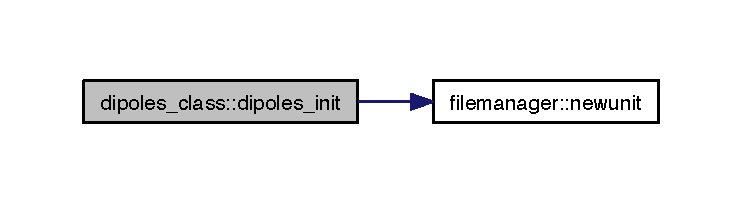
\includegraphics[width=350pt]{classdipoles__class_a947aef5d45c6e39accc6c0e20f619c57_cgraph}
\end{center}
\end{figure}


\hypertarget{classdipoles__class_ab610221599ac72fa22a02617e550033b}{\index{dipoles\+\_\+class@{dipoles\+\_\+class}!dipoles\+\_\+kill@{dipoles\+\_\+kill}}
\index{dipoles\+\_\+kill@{dipoles\+\_\+kill}!dipoles\+\_\+class@{dipoles\+\_\+class}}
\subsubsection[{dipoles\+\_\+kill}]{\setlength{\rightskip}{0pt plus 5cm}subroutine dipoles\+\_\+class\+::dipoles\+\_\+kill (
\begin{DoxyParamCaption}
\item[{type({\bf dipoles}), intent(inout)}]{this}
\end{DoxyParamCaption}
)\hspace{0.3cm}{\ttfamily [private]}}}\label{classdipoles__class_ab610221599ac72fa22a02617e550033b}
\hypertarget{classdipoles__class_a2d80cb493920a4619e0e83abfcb033f6}{\index{dipoles\+\_\+class@{dipoles\+\_\+class}!dipoles\+\_\+resample@{dipoles\+\_\+resample}}
\index{dipoles\+\_\+resample@{dipoles\+\_\+resample}!dipoles\+\_\+class@{dipoles\+\_\+class}}
\subsubsection[{dipoles\+\_\+resample}]{\setlength{\rightskip}{0pt plus 5cm}subroutine dipoles\+\_\+class\+::dipoles\+\_\+resample (
\begin{DoxyParamCaption}
\item[{type({\bf dipoles}), intent(inout)}]{this}
\end{DoxyParamCaption}
)\hspace{0.3cm}{\ttfamily [private]}}}\label{classdipoles__class_a2d80cb493920a4619e0e83abfcb033f6}


Here is the call graph for this function\+:\nopagebreak
\begin{figure}[H]
\begin{center}
\leavevmode
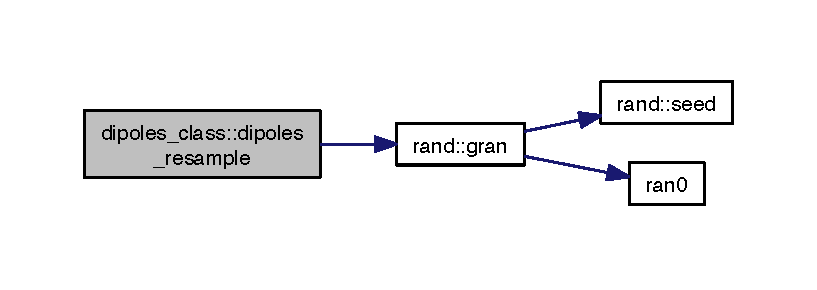
\includegraphics[width=350pt]{classdipoles__class_a2d80cb493920a4619e0e83abfcb033f6_cgraph}
\end{center}
\end{figure}


\hypertarget{classdipoles__class_a9ab428011961577796577f9cdeb032b4}{\index{dipoles\+\_\+class@{dipoles\+\_\+class}!dipoles\+\_\+save@{dipoles\+\_\+save}}
\index{dipoles\+\_\+save@{dipoles\+\_\+save}!dipoles\+\_\+class@{dipoles\+\_\+class}}
\subsubsection[{dipoles\+\_\+save}]{\setlength{\rightskip}{0pt plus 5cm}subroutine dipoles\+\_\+class\+::dipoles\+\_\+save (
\begin{DoxyParamCaption}
\item[{type({\bf dipoles}), intent(in)}]{this, }
\item[{character$\ast$($\ast$), intent(in)}]{file}
\end{DoxyParamCaption}
)\hspace{0.3cm}{\ttfamily [private]}}}\label{classdipoles__class_a9ab428011961577796577f9cdeb032b4}


Here is the call graph for this function\+:\nopagebreak
\begin{figure}[H]
\begin{center}
\leavevmode
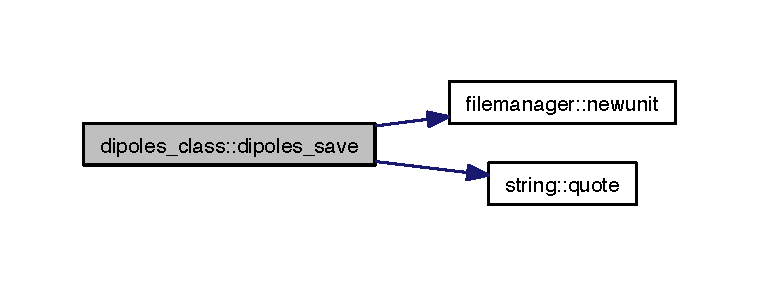
\includegraphics[width=350pt]{classdipoles__class_a9ab428011961577796577f9cdeb032b4_cgraph}
\end{center}
\end{figure}


\hypertarget{classdipoles__class_a9157bf14add87f3f26edfbc88c0da6fe}{\index{dipoles\+\_\+class@{dipoles\+\_\+class}!dipoles\+\_\+update@{dipoles\+\_\+update}}
\index{dipoles\+\_\+update@{dipoles\+\_\+update}!dipoles\+\_\+class@{dipoles\+\_\+class}}
\subsubsection[{dipoles\+\_\+update}]{\setlength{\rightskip}{0pt plus 5cm}subroutine dipoles\+\_\+class\+::dipoles\+\_\+update (
\begin{DoxyParamCaption}
\item[{type({\bf dipoles}), intent(inout)}]{this}
\end{DoxyParamCaption}
)\hspace{0.3cm}{\ttfamily [private]}}}\label{classdipoles__class_a9157bf14add87f3f26edfbc88c0da6fe}


Here is the call graph for this function\+:\nopagebreak
\begin{figure}[H]
\begin{center}
\leavevmode
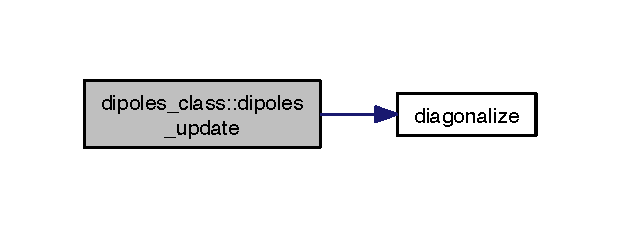
\includegraphics[width=294pt]{classdipoles__class_a9157bf14add87f3f26edfbc88c0da6fe_cgraph}
\end{center}
\end{figure}




The documentation for this module was generated from the following file\+:\begin{DoxyCompactItemize}
\item 
src/\hyperlink{dipoles_8f90}{dipoles.\+f90}\end{DoxyCompactItemize}

\hypertarget{interfaceclassical__class_1_1display}{}\section{classical\+\_\+class\+:\+:display Interface Reference}
\label{interfaceclassical__class_1_1display}\index{classical\+\_\+class\+::display@{classical\+\_\+class\+::display}}
\subsection*{Private Member Functions}
\begin{DoxyCompactItemize}
\item 
subroutine \hyperlink{interfaceclassical__class_1_1display_a38506ee13a51d8f959fcf71976eb13a7}{classical\+\_\+display} (this, msg)
\end{DoxyCompactItemize}


\subsection{Member Function/\+Subroutine Documentation}
\mbox{\Hypertarget{interfaceclassical__class_1_1display_a38506ee13a51d8f959fcf71976eb13a7}\label{interfaceclassical__class_1_1display_a38506ee13a51d8f959fcf71976eb13a7}} 
\index{classical\+\_\+class\+::display@{classical\+\_\+class\+::display}!classical\+\_\+display@{classical\+\_\+display}}
\index{classical\+\_\+display@{classical\+\_\+display}!classical\+\_\+class\+::display@{classical\+\_\+class\+::display}}
\subsubsection{\texorpdfstring{classical\+\_\+display()}{classical\_display()}}
{\footnotesize\ttfamily subroutine classical\+\_\+class\+::display\+::classical\+\_\+display (\begin{DoxyParamCaption}\item[{type(\hyperlink{structclassical__class_1_1classical}{classical}), intent(in)}]{this,  }\item[{character$\ast$($\ast$), intent(in), optional}]{msg }\end{DoxyParamCaption})\hspace{0.3cm}{\ttfamily [private]}}



The documentation for this interface was generated from the following file\+:\begin{DoxyCompactItemize}
\item 
src/\hyperlink{classical_8f90}{classical.\+f90}\end{DoxyCompactItemize}

\hypertarget{interfacedipoles__class_1_1display}{}\section{dipoles\+\_\+class\+:\+:display Interface Reference}
\label{interfacedipoles__class_1_1display}\index{dipoles\+\_\+class\+::display@{dipoles\+\_\+class\+::display}}
\subsection*{Private Member Functions}
\begin{DoxyCompactItemize}
\item 
subroutine \hyperlink{interfacedipoles__class_1_1display_a3d1f4136682f30287af165a4a28496e6}{dipoles\+\_\+display} (this, msg)
\end{DoxyCompactItemize}


\subsection{Member Function/\+Subroutine Documentation}
\mbox{\Hypertarget{interfacedipoles__class_1_1display_a3d1f4136682f30287af165a4a28496e6}\label{interfacedipoles__class_1_1display_a3d1f4136682f30287af165a4a28496e6}} 
\index{dipoles\+\_\+class\+::display@{dipoles\+\_\+class\+::display}!dipoles\+\_\+display@{dipoles\+\_\+display}}
\index{dipoles\+\_\+display@{dipoles\+\_\+display}!dipoles\+\_\+class\+::display@{dipoles\+\_\+class\+::display}}
\subsubsection{\texorpdfstring{dipoles\+\_\+display()}{dipoles\_display()}}
{\footnotesize\ttfamily subroutine dipoles\+\_\+class\+::display\+::dipoles\+\_\+display (\begin{DoxyParamCaption}\item[{type(\hyperlink{structdipoles__class_1_1dipoles}{dipoles}), intent(in)}]{this,  }\item[{character$\ast$($\ast$), intent(in), optional}]{msg }\end{DoxyParamCaption})\hspace{0.3cm}{\ttfamily [private]}}



The documentation for this interface was generated from the following file\+:\begin{DoxyCompactItemize}
\item 
src/\hyperlink{dipoles_8f90}{dipoles.\+f90}\end{DoxyCompactItemize}

\hypertarget{interfaceoutputdisplay_1_1display}{\section{outputdisplay\+:\+:display Interface Reference}
\label{interfaceoutputdisplay_1_1display}\index{outputdisplay\+::display@{outputdisplay\+::display}}
}
\subsection*{Private Member Functions}
\begin{DoxyCompactItemize}
\item 
subroutine \hyperlink{interfaceoutputdisplay_1_1display_a9485418eb16aaf7a4db51a046574d6de}{display\+\_\+init} (file)
\begin{DoxyCompactList}\small\item\em redirects display output to newfile \end{DoxyCompactList}\end{DoxyCompactItemize}


\subsection{Member Function/\+Subroutine Documentation}
\hypertarget{interfaceoutputdisplay_1_1display_a9485418eb16aaf7a4db51a046574d6de}{\index{outputdisplay\+::display@{outputdisplay\+::display}!display\+\_\+init@{display\+\_\+init}}
\index{display\+\_\+init@{display\+\_\+init}!outputdisplay\+::display@{outputdisplay\+::display}}
\subsubsection[{display\+\_\+init}]{\setlength{\rightskip}{0pt plus 5cm}subroutine outputdisplay\+::display\+::display\+\_\+init (
\begin{DoxyParamCaption}
\item[{character$\ast$($\ast$), intent(in)}]{file}
\end{DoxyParamCaption}
)\hspace{0.3cm}{\ttfamily [private]}}}\label{interfaceoutputdisplay_1_1display_a9485418eb16aaf7a4db51a046574d6de}


redirects display output to newfile 



The documentation for this interface was generated from the following file\+:\begin{DoxyCompactItemize}
\item 
src/\hyperlink{utils_8f90}{utils.\+f90}\end{DoxyCompactItemize}

\hypertarget{interfacehs__class_1_1display}{\section{hs\-\_\-class\-:\-:display Interface Reference}
\label{interfacehs__class_1_1display}\index{hs\-\_\-class\-::display@{hs\-\_\-class\-::display}}
}


Prints out current state of the hs type.  


\subsection*{Private Member Functions}
\begin{DoxyCompactItemize}
\item 
subroutine \hyperlink{interfacehs__class_1_1display_a6f6551ea4371aca98c85f1f83600a422}{hs\-\_\-display} (this, msg)
\end{DoxyCompactItemize}


\subsection{Detailed Description}
Prints out current state of the hs type. 

\subsection{Member Function/\-Subroutine Documentation}
\hypertarget{interfacehs__class_1_1display_a6f6551ea4371aca98c85f1f83600a422}{\index{hs\-\_\-class\-::display@{hs\-\_\-class\-::display}!hs\-\_\-display@{hs\-\_\-display}}
\index{hs\-\_\-display@{hs\-\_\-display}!hs_class::display@{hs\-\_\-class\-::display}}
\subsubsection[{hs\-\_\-display}]{\setlength{\rightskip}{0pt plus 5cm}subroutine hs\-\_\-class\-::display\-::hs\-\_\-display (
\begin{DoxyParamCaption}
\item[{type({\bf hs}), intent(in)}]{this, }
\item[{character$\ast$($\ast$), intent(in), optional}]{msg}
\end{DoxyParamCaption}
)\hspace{0.3cm}{\ttfamily [private]}}}\label{interfacehs__class_1_1display_a6f6551ea4371aca98c85f1f83600a422}


The documentation for this interface was generated from the following file\-:\begin{DoxyCompactItemize}
\item 
src/\hyperlink{hs_8f90}{hs.\-f90}\end{DoxyCompactItemize}

\hypertarget{interfacetextgraphs_1_1display}{}\section{textgraphs\+:\+:display Interface Reference}
\label{interfacetextgraphs_1_1display}\index{textgraphs\+::display@{textgraphs\+::display}}
\subsection*{Private Member Functions}
\begin{DoxyCompactItemize}
\item 
subroutine \hyperlink{interfacetextgraphs_1_1display_ad87a2b0b95d37672aac96a547592b374}{displaycmplxmatrix} (Z, tol, msg)
\begin{DoxyCompactList}\small\item\em Plot Complex Matrix. \end{DoxyCompactList}\item 
subroutine \hyperlink{interfacetextgraphs_1_1display_a234a24e4326c818c2f2e274e8e3a1bee}{displayrealmatrix} (A, tol, msg)
\begin{DoxyCompactList}\small\item\em Plot Real Matrix. \end{DoxyCompactList}\item 
subroutine \hyperlink{interfacetextgraphs_1_1display_a2c20d3e1fdb1272f9bf904e114c21313}{displayvectfield} (Q, Mu, tol, nptx, npty, labelvect, msg)
\begin{DoxyCompactList}\small\item\em Plot Vector Field. \end{DoxyCompactList}\item 
subroutine \hyperlink{interfacetextgraphs_1_1display_ac47b1a55cfdca825dd26ca969ab5bf38}{displayvalues} (Q, npt, msg)
\begin{DoxyCompactList}\small\item\em Display Array Vaules. \end{DoxyCompactList}\item 
subroutine \hyperlink{interfacetextgraphs_1_1display_a490c583611a481c4a4ee80a1d8bd2b36}{displayxy} (Xset, Yset, nptx, npty, mask, msg)
\begin{DoxyCompactList}\small\item\em Scatter plot details/ displays xy data as nptx x npty char text. \end{DoxyCompactList}\end{DoxyCompactItemize}


\subsection{Member Function/\+Subroutine Documentation}
\mbox{\Hypertarget{interfacetextgraphs_1_1display_ad87a2b0b95d37672aac96a547592b374}\label{interfacetextgraphs_1_1display_ad87a2b0b95d37672aac96a547592b374}} 
\index{textgraphs\+::display@{textgraphs\+::display}!displaycmplxmatrix@{displaycmplxmatrix}}
\index{displaycmplxmatrix@{displaycmplxmatrix}!textgraphs\+::display@{textgraphs\+::display}}
\subsubsection{\texorpdfstring{displaycmplxmatrix()}{displaycmplxmatrix()}}
{\footnotesize\ttfamily subroutine textgraphs\+::display\+::displaycmplxmatrix (\begin{DoxyParamCaption}\item[{complex(double), dimension(\+:,\+:), intent(in), target}]{Z,  }\item[{real(double), intent(in), optional}]{tol,  }\item[{character$\ast$($\ast$), intent(in), optional}]{msg }\end{DoxyParamCaption})\hspace{0.3cm}{\ttfamily [private]}}



Plot Complex Matrix. 

Displays a 2D complex matrix elements as 2 char text in NxM table, where N and M are the dimensions of the input matrix. \mbox{\Hypertarget{interfacetextgraphs_1_1display_a234a24e4326c818c2f2e274e8e3a1bee}\label{interfacetextgraphs_1_1display_a234a24e4326c818c2f2e274e8e3a1bee}} 
\index{textgraphs\+::display@{textgraphs\+::display}!displayrealmatrix@{displayrealmatrix}}
\index{displayrealmatrix@{displayrealmatrix}!textgraphs\+::display@{textgraphs\+::display}}
\subsubsection{\texorpdfstring{displayrealmatrix()}{displayrealmatrix()}}
{\footnotesize\ttfamily subroutine textgraphs\+::display\+::displayrealmatrix (\begin{DoxyParamCaption}\item[{real(double), dimension(\+:,\+:), intent(in), target}]{A,  }\item[{real(double), intent(in), optional}]{tol,  }\item[{character$\ast$($\ast$), intent(in), optional}]{msg }\end{DoxyParamCaption})\hspace{0.3cm}{\ttfamily [private]}}



Plot Real Matrix. 

Displays a 2D real matrix elements as 1 char text in NxM table, where N and M are the dimensions of the input matrix. \mbox{\Hypertarget{interfacetextgraphs_1_1display_ac47b1a55cfdca825dd26ca969ab5bf38}\label{interfacetextgraphs_1_1display_ac47b1a55cfdca825dd26ca969ab5bf38}} 
\index{textgraphs\+::display@{textgraphs\+::display}!displayvalues@{displayvalues}}
\index{displayvalues@{displayvalues}!textgraphs\+::display@{textgraphs\+::display}}
\subsubsection{\texorpdfstring{displayvalues()}{displayvalues()}}
{\footnotesize\ttfamily subroutine textgraphs\+::display\+::displayvalues (\begin{DoxyParamCaption}\item[{real(double), dimension(\+:), intent(in), target}]{Q,  }\item[{integer(long), intent(in), optional}]{npt,  }\item[{character$\ast$($\ast$), intent(in), optional}]{msg }\end{DoxyParamCaption})\hspace{0.3cm}{\ttfamily [private]}}



Display Array Vaules. 

Plots a function contained in Q with text each element of Q gets a character on a the record with npt represents the range of values \mbox{\Hypertarget{interfacetextgraphs_1_1display_a2c20d3e1fdb1272f9bf904e114c21313}\label{interfacetextgraphs_1_1display_a2c20d3e1fdb1272f9bf904e114c21313}} 
\index{textgraphs\+::display@{textgraphs\+::display}!displayvectfield@{displayvectfield}}
\index{displayvectfield@{displayvectfield}!textgraphs\+::display@{textgraphs\+::display}}
\subsubsection{\texorpdfstring{displayvectfield()}{displayvectfield()}}
{\footnotesize\ttfamily subroutine textgraphs\+::display\+::displayvectfield (\begin{DoxyParamCaption}\item[{real(double), dimension(\+:,\+:), intent(in), target}]{Q,  }\item[{real(double), dimension(\+:,\+:), intent(in), target}]{Mu,  }\item[{real(double), intent(in), optional}]{tol,  }\item[{integer(long), intent(in), optional}]{nptx,  }\item[{integer(long), intent(in), optional}]{npty,  }\item[{logical, intent(in), optional}]{labelvect,  }\item[{character$\ast$($\ast$), intent(in), optional}]{msg }\end{DoxyParamCaption})\hspace{0.3cm}{\ttfamily [private]}}



Plot Vector Field. 

Displays a 2D vector field elements as nptx x npty char text. \mbox{\Hypertarget{interfacetextgraphs_1_1display_a490c583611a481c4a4ee80a1d8bd2b36}\label{interfacetextgraphs_1_1display_a490c583611a481c4a4ee80a1d8bd2b36}} 
\index{textgraphs\+::display@{textgraphs\+::display}!displayxy@{displayxy}}
\index{displayxy@{displayxy}!textgraphs\+::display@{textgraphs\+::display}}
\subsubsection{\texorpdfstring{displayxy()}{displayxy()}}
{\footnotesize\ttfamily subroutine textgraphs\+::display\+::displayxy (\begin{DoxyParamCaption}\item[{real(double), dimension(\+:), intent(in), target}]{Xset,  }\item[{real(double), dimension(\+:), intent(in), target}]{Yset,  }\item[{integer(long), intent(in), optional}]{nptx,  }\item[{integer(long), intent(in), optional}]{npty,  }\item[{logical, dimension(\+:), intent(in), optional}]{mask,  }\item[{character$\ast$($\ast$), intent(in), optional}]{msg }\end{DoxyParamCaption})\hspace{0.3cm}{\ttfamily [private]}}



Scatter plot details/ displays xy data as nptx x npty char text. 



The documentation for this interface was generated from the following file\+:\begin{DoxyCompactItemize}
\item 
src/\hyperlink{utils_8f90}{utils.\+f90}\end{DoxyCompactItemize}

\hypertarget{interfaceharmonicbath__class_1_1display}{}\section{harmonicbath\+\_\+class\+:\+:display Interface Reference}
\label{interfaceharmonicbath__class_1_1display}\index{harmonicbath\+\_\+class\+::display@{harmonicbath\+\_\+class\+::display}}
\subsection*{Private Member Functions}
\begin{DoxyCompactItemize}
\item 
subroutine \hyperlink{interfaceharmonicbath__class_1_1display_ac470b2ebb72ec1bc947b5874a9cc2155}{harmonicbath\+\_\+display} (this, msg)
\end{DoxyCompactItemize}


\subsection{Member Function/\+Subroutine Documentation}
\mbox{\Hypertarget{interfaceharmonicbath__class_1_1display_ac470b2ebb72ec1bc947b5874a9cc2155}\label{interfaceharmonicbath__class_1_1display_ac470b2ebb72ec1bc947b5874a9cc2155}} 
\index{harmonicbath\+\_\+class\+::display@{harmonicbath\+\_\+class\+::display}!harmonicbath\+\_\+display@{harmonicbath\+\_\+display}}
\index{harmonicbath\+\_\+display@{harmonicbath\+\_\+display}!harmonicbath\+\_\+class\+::display@{harmonicbath\+\_\+class\+::display}}
\subsubsection{\texorpdfstring{harmonicbath\+\_\+display()}{harmonicbath\_display()}}
{\footnotesize\ttfamily subroutine harmonicbath\+\_\+class\+::display\+::harmonicbath\+\_\+display (\begin{DoxyParamCaption}\item[{type(\hyperlink{structharmonicbath__class_1_1harmonicbath}{harmonicbath}), intent(in)}]{this,  }\item[{character$\ast$($\ast$), intent(in), optional}]{msg }\end{DoxyParamCaption})\hspace{0.3cm}{\ttfamily [private]}}



The documentation for this interface was generated from the following file\+:\begin{DoxyCompactItemize}
\item 
src/\hyperlink{harmonicbath_8f90}{harmonicbath.\+f90}\end{DoxyCompactItemize}

\hypertarget{interfacemolreader_1_1display}{}\section{molreader\+:\+:display Interface Reference}
\label{interfacemolreader_1_1display}\index{molreader\+::display@{molreader\+::display}}
\subsection*{Private Member Functions}
\begin{DoxyCompactItemize}
\item 
subroutine \hyperlink{interfacemolreader_1_1display_a367a91877524a939c53cd58ce8ac0635}{display\+\_\+cryst1} (this, unit)
\item 
subroutine \hyperlink{interfacemolreader_1_1display_af76b8884f32bae6a2a70d92dea1e884d}{display\+\_\+model} (this, unit)
\item 
subroutine \hyperlink{interfacemolreader_1_1display_a9e155fe19986dcbbceeccb957eb9eedb}{display\+\_\+atom} (this, unit)
\item 
subroutine \hyperlink{interfacemolreader_1_1display_a0f0d826e10fcae2957860b21580f136a}{display\+\_\+psfatom} (this, unit)
\end{DoxyCompactItemize}


\subsection{Member Function/\+Subroutine Documentation}
\mbox{\Hypertarget{interfacemolreader_1_1display_a9e155fe19986dcbbceeccb957eb9eedb}\label{interfacemolreader_1_1display_a9e155fe19986dcbbceeccb957eb9eedb}} 
\index{molreader\+::display@{molreader\+::display}!display\+\_\+atom@{display\+\_\+atom}}
\index{display\+\_\+atom@{display\+\_\+atom}!molreader\+::display@{molreader\+::display}}
\subsubsection{\texorpdfstring{display\+\_\+atom()}{display\_atom()}}
{\footnotesize\ttfamily subroutine molreader\+::display\+::display\+\_\+atom (\begin{DoxyParamCaption}\item[{type(\hyperlink{structmolreader_1_1atom}{atom}), intent(inout)}]{this,  }\item[{integer(long), optional}]{unit }\end{DoxyParamCaption})\hspace{0.3cm}{\ttfamily [private]}}

\mbox{\Hypertarget{interfacemolreader_1_1display_a367a91877524a939c53cd58ce8ac0635}\label{interfacemolreader_1_1display_a367a91877524a939c53cd58ce8ac0635}} 
\index{molreader\+::display@{molreader\+::display}!display\+\_\+cryst1@{display\+\_\+cryst1}}
\index{display\+\_\+cryst1@{display\+\_\+cryst1}!molreader\+::display@{molreader\+::display}}
\subsubsection{\texorpdfstring{display\+\_\+cryst1()}{display\_cryst1()}}
{\footnotesize\ttfamily subroutine molreader\+::display\+::display\+\_\+cryst1 (\begin{DoxyParamCaption}\item[{type(\hyperlink{structmolreader_1_1cryst1}{cryst1}), intent(inout)}]{this,  }\item[{integer(long), optional}]{unit }\end{DoxyParamCaption})\hspace{0.3cm}{\ttfamily [private]}}

\mbox{\Hypertarget{interfacemolreader_1_1display_af76b8884f32bae6a2a70d92dea1e884d}\label{interfacemolreader_1_1display_af76b8884f32bae6a2a70d92dea1e884d}} 
\index{molreader\+::display@{molreader\+::display}!display\+\_\+model@{display\+\_\+model}}
\index{display\+\_\+model@{display\+\_\+model}!molreader\+::display@{molreader\+::display}}
\subsubsection{\texorpdfstring{display\+\_\+model()}{display\_model()}}
{\footnotesize\ttfamily subroutine molreader\+::display\+::display\+\_\+model (\begin{DoxyParamCaption}\item[{type(\hyperlink{structmolreader_1_1model}{model}), intent(inout)}]{this,  }\item[{integer(long), optional}]{unit }\end{DoxyParamCaption})\hspace{0.3cm}{\ttfamily [private]}}

\mbox{\Hypertarget{interfacemolreader_1_1display_a0f0d826e10fcae2957860b21580f136a}\label{interfacemolreader_1_1display_a0f0d826e10fcae2957860b21580f136a}} 
\index{molreader\+::display@{molreader\+::display}!display\+\_\+psfatom@{display\+\_\+psfatom}}
\index{display\+\_\+psfatom@{display\+\_\+psfatom}!molreader\+::display@{molreader\+::display}}
\subsubsection{\texorpdfstring{display\+\_\+psfatom()}{display\_psfatom()}}
{\footnotesize\ttfamily subroutine molreader\+::display\+::display\+\_\+psfatom (\begin{DoxyParamCaption}\item[{type(\hyperlink{structmolreader_1_1psfatom}{psfatom}), intent(in)}]{this,  }\item[{integer(long), optional}]{unit }\end{DoxyParamCaption})\hspace{0.3cm}{\ttfamily [private]}}



The documentation for this interface was generated from the following file\+:\begin{DoxyCompactItemize}
\item 
src/\hyperlink{molreader_8f90}{molreader.\+f90}\end{DoxyCompactItemize}

\hypertarget{interfacepldm__class_1_1display}{\section{pldm\-\_\-class\-:\-:display Interface Reference}
\label{interfacepldm__class_1_1display}\index{pldm\-\_\-class\-::display@{pldm\-\_\-class\-::display}}
}
\subsection*{Private Member Functions}
\begin{DoxyCompactItemize}
\item 
subroutine \hyperlink{interfacepldm__class_1_1display_afb1b71e41434371ec0eaab02cee36d48}{pldm\-\_\-display} (this)
\end{DoxyCompactItemize}


\subsection{Member Function/\-Subroutine Documentation}
\hypertarget{interfacepldm__class_1_1display_afb1b71e41434371ec0eaab02cee36d48}{\index{pldm\-\_\-class\-::display@{pldm\-\_\-class\-::display}!pldm\-\_\-display@{pldm\-\_\-display}}
\index{pldm\-\_\-display@{pldm\-\_\-display}!pldm_class::display@{pldm\-\_\-class\-::display}}
\subsubsection[{pldm\-\_\-display}]{\setlength{\rightskip}{0pt plus 5cm}subroutine pldm\-\_\-class\-::display\-::pldm\-\_\-display (
\begin{DoxyParamCaption}
\item[{type({\bf pldm}), intent(in)}]{this}
\end{DoxyParamCaption}
)\hspace{0.3cm}{\ttfamily [private]}}}\label{interfacepldm__class_1_1display_afb1b71e41434371ec0eaab02cee36d48}


The documentation for this interface was generated from the following file\-:\begin{DoxyCompactItemize}
\item 
src/\hyperlink{_p_l_d_m_8f90}{P\-L\-D\-M.\-f90}\end{DoxyCompactItemize}

\hypertarget{interfacequantum__class_1_1display}{\section{quantum\-\_\-class\-:\-:display Interface Reference}
\label{interfacequantum__class_1_1display}\index{quantum\-\_\-class\-::display@{quantum\-\_\-class\-::display}}
}
\subsection*{Private Member Functions}
\begin{DoxyCompactItemize}
\item 
subroutine \hyperlink{interfacequantum__class_1_1display_ac7c738dc00158d70772a5930d1dab58e}{quantum\-\_\-display} (this, msg)
\end{DoxyCompactItemize}


\subsection{Member Function/\-Subroutine Documentation}
\hypertarget{interfacequantum__class_1_1display_ac7c738dc00158d70772a5930d1dab58e}{\index{quantum\-\_\-class\-::display@{quantum\-\_\-class\-::display}!quantum\-\_\-display@{quantum\-\_\-display}}
\index{quantum\-\_\-display@{quantum\-\_\-display}!quantum_class::display@{quantum\-\_\-class\-::display}}
\subsubsection[{quantum\-\_\-display}]{\setlength{\rightskip}{0pt plus 5cm}subroutine quantum\-\_\-class\-::display\-::quantum\-\_\-display (
\begin{DoxyParamCaption}
\item[{type({\bf quantum}), intent(in)}]{this, }
\item[{character$\ast$($\ast$), intent(in), optional}]{msg}
\end{DoxyParamCaption}
)\hspace{0.3cm}{\ttfamily [private]}}}\label{interfacequantum__class_1_1display_ac7c738dc00158d70772a5930d1dab58e}


The documentation for this interface was generated from the following file\-:\begin{DoxyCompactItemize}
\item 
src/\hyperlink{quantum_8f90}{quantum.\-f90}\end{DoxyCompactItemize}

\hypertarget{interfacespectrometer__class_1_1display}{\section{spectrometer\-\_\-class\-:\-:display Interface Reference}
\label{interfacespectrometer__class_1_1display}\index{spectrometer\-\_\-class\-::display@{spectrometer\-\_\-class\-::display}}
}


Display the spectrum type.  


\subsection*{Private Member Functions}
\begin{DoxyCompactItemize}
\item 
subroutine \hyperlink{interfacespectrometer__class_1_1display_ad2a5c61a3b9a1a59d5fc73d97e3141ff}{display\-\_\-spectrum} (this)
\end{DoxyCompactItemize}


\subsection{Detailed Description}
Display the spectrum type. 

\subsection{Member Function/\-Subroutine Documentation}
\hypertarget{interfacespectrometer__class_1_1display_ad2a5c61a3b9a1a59d5fc73d97e3141ff}{\index{spectrometer\-\_\-class\-::display@{spectrometer\-\_\-class\-::display}!display\-\_\-spectrum@{display\-\_\-spectrum}}
\index{display\-\_\-spectrum@{display\-\_\-spectrum}!spectrometer_class::display@{spectrometer\-\_\-class\-::display}}
\subsubsection[{display\-\_\-spectrum}]{\setlength{\rightskip}{0pt plus 5cm}subroutine spectrometer\-\_\-class\-::display\-::display\-\_\-spectrum (
\begin{DoxyParamCaption}
\item[{type({\bf spectrum}), intent(inout)}]{this}
\end{DoxyParamCaption}
)\hspace{0.3cm}{\ttfamily [private]}}}\label{interfacespectrometer__class_1_1display_ad2a5c61a3b9a1a59d5fc73d97e3141ff}


The documentation for this interface was generated from the following file\-:\begin{DoxyCompactItemize}
\item 
src/\hyperlink{spectrometer_8f90}{spectrometer.\-f90}\end{DoxyCompactItemize}

\hypertarget{interfacebilinear__class_1_1display}{}\section{bilinear\+\_\+class\+:\+:display Interface Reference}
\label{interfacebilinear__class_1_1display}\index{bilinear\+\_\+class\+::display@{bilinear\+\_\+class\+::display}}


Displays the current state of the bilinear object.  


\subsection*{Private Member Functions}
\begin{DoxyCompactItemize}
\item 
subroutine \hyperlink{interfacebilinear__class_1_1display_a91e66fb870373dafc2fcb58a17a88fdb}{bilinear\+\_\+display} (this, msg)
\begin{DoxyCompactList}\small\item\em Displays the bilinear coupling object. \end{DoxyCompactList}\end{DoxyCompactItemize}


\subsection{Detailed Description}
Displays the current state of the bilinear object. 

\subsection{Member Function/\+Subroutine Documentation}
\mbox{\Hypertarget{interfacebilinear__class_1_1display_a91e66fb870373dafc2fcb58a17a88fdb}\label{interfacebilinear__class_1_1display_a91e66fb870373dafc2fcb58a17a88fdb}} 
\index{bilinear\+\_\+class\+::display@{bilinear\+\_\+class\+::display}!bilinear\+\_\+display@{bilinear\+\_\+display}}
\index{bilinear\+\_\+display@{bilinear\+\_\+display}!bilinear\+\_\+class\+::display@{bilinear\+\_\+class\+::display}}
\subsubsection{\texorpdfstring{bilinear\+\_\+display()}{bilinear\_display()}}
{\footnotesize\ttfamily subroutine bilinear\+\_\+class\+::display\+::bilinear\+\_\+display (\begin{DoxyParamCaption}\item[{type(\hyperlink{structbilinear__class_1_1bilinear}{bilinear}), intent(in)}]{this,  }\item[{character$\ast$($\ast$), intent(in), optional}]{msg }\end{DoxyParamCaption})\hspace{0.3cm}{\ttfamily [private]}}



Displays the bilinear coupling object. 


\begin{DoxyParams}[1]{Parameters}
\mbox{\tt in}  & {\em this} & is the bilinear coupling object to be checked. \\
\hline
\end{DoxyParams}
\begin{DoxyReturn}{Returns}
Nothing if all checks pass or 1 and a warn for the first failed check. 
\end{DoxyReturn}
\begin{DoxyRemark}{Remarks}
Will exit after first failed check. 
\end{DoxyRemark}


The documentation for this interface was generated from the following file\+:\begin{DoxyCompactItemize}
\item 
src/\hyperlink{bilinear_8f90}{bilinear.\+f90}\end{DoxyCompactItemize}

\hypertarget{interfacehb__class_1_1display}{\section{hb\+\_\+class\+:\+:display Interface Reference}
\label{interfacehb__class_1_1display}\index{hb\+\_\+class\+::display@{hb\+\_\+class\+::display}}
}
\subsection*{Private Member Functions}
\begin{DoxyCompactItemize}
\item 
subroutine \hyperlink{interfacehb__class_1_1display_ac9bf2c27966be0c6535716e8603f22aa}{hb\+\_\+display} (this, msg)
\item 
subroutine \hyperlink{interfacehb__class_1_1display_ac9bf2c27966be0c6535716e8603f22aa}{hb\+\_\+display} (this, msg)
\end{DoxyCompactItemize}


\subsection{Member Function/\+Subroutine Documentation}
\hypertarget{interfacehb__class_1_1display_ac9bf2c27966be0c6535716e8603f22aa}{\index{hb\+\_\+class\+::display@{hb\+\_\+class\+::display}!hb\+\_\+display@{hb\+\_\+display}}
\index{hb\+\_\+display@{hb\+\_\+display}!hb\+\_\+class\+::display@{hb\+\_\+class\+::display}}
\subsubsection[{hb\+\_\+display}]{\setlength{\rightskip}{0pt plus 5cm}subroutine hb\+\_\+class\+::display\+::hb\+\_\+display (
\begin{DoxyParamCaption}
\item[{type({\bf hb}), intent(in)}]{this, }
\item[{character$\ast$($\ast$), intent(in), optional}]{msg}
\end{DoxyParamCaption}
)\hspace{0.3cm}{\ttfamily [private]}}}\label{interfacehb__class_1_1display_ac9bf2c27966be0c6535716e8603f22aa}
\hypertarget{interfacehb__class_1_1display_ac9bf2c27966be0c6535716e8603f22aa}{\index{hb\+\_\+class\+::display@{hb\+\_\+class\+::display}!hb\+\_\+display@{hb\+\_\+display}}
\index{hb\+\_\+display@{hb\+\_\+display}!hb\+\_\+class\+::display@{hb\+\_\+class\+::display}}
\subsubsection[{hb\+\_\+display}]{\setlength{\rightskip}{0pt plus 5cm}subroutine hb\+\_\+class\+::display\+::hb\+\_\+display (
\begin{DoxyParamCaption}
\item[{type({\bf hb}), intent(in)}]{this, }
\item[{character$\ast$($\ast$), intent(in), optional}]{msg}
\end{DoxyParamCaption}
)\hspace{0.3cm}{\ttfamily [private]}}}\label{interfacehb__class_1_1display_ac9bf2c27966be0c6535716e8603f22aa}


The documentation for this interface was generated from the following files\+:\begin{DoxyCompactItemize}
\item 
src/\hyperlink{hb_8f90}{hb.\+f90}\item 
src/\hyperlink{hbcopy_8f90}{hbcopy.\+f90}\end{DoxyCompactItemize}

\hypertarget{interfacecoupling__class_1_1display}{}\section{coupling\+\_\+class\+:\+:display Interface Reference}
\label{interfacecoupling__class_1_1display}\index{coupling\+\_\+class\+::display@{coupling\+\_\+class\+::display}}
\subsection*{Private Member Functions}
\begin{DoxyCompactItemize}
\item 
subroutine \hyperlink{interfacecoupling__class_1_1display_a4b78570031cdb831119d6a140a1aa55b}{coupling\+\_\+display} (this, msg)
\end{DoxyCompactItemize}


\subsection{Member Function/\+Subroutine Documentation}
\mbox{\Hypertarget{interfacecoupling__class_1_1display_a4b78570031cdb831119d6a140a1aa55b}\label{interfacecoupling__class_1_1display_a4b78570031cdb831119d6a140a1aa55b}} 
\index{coupling\+\_\+class\+::display@{coupling\+\_\+class\+::display}!coupling\+\_\+display@{coupling\+\_\+display}}
\index{coupling\+\_\+display@{coupling\+\_\+display}!coupling\+\_\+class\+::display@{coupling\+\_\+class\+::display}}
\subsubsection{\texorpdfstring{coupling\+\_\+display()}{coupling\_display()}}
{\footnotesize\ttfamily subroutine coupling\+\_\+class\+::display\+::coupling\+\_\+display (\begin{DoxyParamCaption}\item[{type(\hyperlink{structcoupling__class_1_1coupling}{coupling}), intent(in)}]{this,  }\item[{character$\ast$($\ast$), intent(in), optional}]{msg }\end{DoxyParamCaption})\hspace{0.3cm}{\ttfamily [private]}}



The documentation for this interface was generated from the following file\+:\begin{DoxyCompactItemize}
\item 
src/\hyperlink{coupling_8f90}{coupling.\+f90}\end{DoxyCompactItemize}

\hypertarget{interfacetemplate__class_1_1display}{\section{template\-\_\-class\-:\-:display Interface Reference}
\label{interfacetemplate__class_1_1display}\index{template\-\_\-class\-::display@{template\-\_\-class\-::display}}
}


Displays the current state of the T\-E\-M\-P\-L\-A\-T\-E object.  


\subsection*{Private Member Functions}
\begin{DoxyCompactItemize}
\item 
subroutine \hyperlink{interfacetemplate__class_1_1display_aedd91f472026140560fdadc2117ed68c}{template\-\_\-display} (this, msg)
\begin{DoxyCompactList}\small\item\em Checks the T\-E\-M\-P\-L\-A\-T\-E object. \end{DoxyCompactList}\end{DoxyCompactItemize}


\subsection{Detailed Description}
Displays the current state of the T\-E\-M\-P\-L\-A\-T\-E object. 

\subsection{Member Function/\-Subroutine Documentation}
\hypertarget{interfacetemplate__class_1_1display_aedd91f472026140560fdadc2117ed68c}{\index{template\-\_\-class\-::display@{template\-\_\-class\-::display}!template\-\_\-display@{template\-\_\-display}}
\index{template\-\_\-display@{template\-\_\-display}!template_class::display@{template\-\_\-class\-::display}}
\subsubsection[{template\-\_\-display}]{\setlength{\rightskip}{0pt plus 5cm}subroutine template\-\_\-class\-::display\-::template\-\_\-display (
\begin{DoxyParamCaption}
\item[{type({\bf template}), intent(in)}]{this, }
\item[{character$\ast$($\ast$), intent(in), optional}]{msg}
\end{DoxyParamCaption}
)\hspace{0.3cm}{\ttfamily [private]}}}\label{interfacetemplate__class_1_1display_aedd91f472026140560fdadc2117ed68c}


Checks the T\-E\-M\-P\-L\-A\-T\-E object. 


\begin{DoxyParams}[1]{Parameters}
\mbox{\tt in}  & {\em this} & is the T\-E\-M\-P\-L\-A\-T\-E object to be updated. \\
\hline
\mbox{\tt in}  & {\em msg} & is an optional string message to preface the displayed object. \\
\hline
\end{DoxyParams}


The documentation for this interface was generated from the following file\-:\begin{DoxyCompactItemize}
\item 
src/\hyperlink{_t_e_m_p_l_a_t_e_8f90}{T\-E\-M\-P\-L\-A\-T\-E.\-f90}\end{DoxyCompactItemize}

\hypertarget{interfacehc__class_1_1display}{\section{hc\-\_\-class\-:\-:display Interface Reference}
\label{interfacehc__class_1_1display}\index{hc\-\_\-class\-::display@{hc\-\_\-class\-::display}}
}
\subsection*{Private Member Functions}
\begin{DoxyCompactItemize}
\item 
subroutine \hyperlink{interfacehc__class_1_1display_a319cf8e35b038638641be5c2b4510eb4}{hc\-\_\-display} (this, msg)
\end{DoxyCompactItemize}


\subsection{Member Function/\-Subroutine Documentation}
\hypertarget{interfacehc__class_1_1display_a319cf8e35b038638641be5c2b4510eb4}{\index{hc\-\_\-class\-::display@{hc\-\_\-class\-::display}!hc\-\_\-display@{hc\-\_\-display}}
\index{hc\-\_\-display@{hc\-\_\-display}!hc_class::display@{hc\-\_\-class\-::display}}
\subsubsection[{hc\-\_\-display}]{\setlength{\rightskip}{0pt plus 5cm}subroutine hc\-\_\-class\-::display\-::hc\-\_\-display (
\begin{DoxyParamCaption}
\item[{type({\bf hc}), intent(in)}]{this, }
\item[{character$\ast$($\ast$), intent(in), optional}]{msg}
\end{DoxyParamCaption}
)\hspace{0.3cm}{\ttfamily [private]}}}\label{interfacehc__class_1_1display_a319cf8e35b038638641be5c2b4510eb4}


The documentation for this interface was generated from the following file\-:\begin{DoxyCompactItemize}
\item 
src/\hyperlink{hc_8f90}{hc.\-f90}\end{DoxyCompactItemize}

\hypertarget{classerrorlog}{\section{errorlog Module Reference}
\label{classerrorlog}\index{errorlog@{errorlog}}
}


Error Handleing.  


\subsection*{Data Types}
\begin{DoxyCompactItemize}
\item 
interface \hyperlink{interfaceerrorlog_1_1note}{note}
\item 
interface \hyperlink{interfaceerrorlog_1_1prompt}{prompt}
\item 
interface \hyperlink{interfaceerrorlog_1_1stop}{stop}
\item 
interface \hyperlink{interfaceerrorlog_1_1warn}{warn}
\end{DoxyCompactItemize}
\subsection*{Public Member Functions}
\begin{DoxyCompactItemize}
\item 
subroutine, public \hyperlink{classerrorlog_a05d233f410ba88bf3e2929528b1bb91e}{displaylog}
\item 
subroutine, public \hyperlink{classerrorlog_a32bbf87dd265de25bd10ea31d95b751d}{openlog} (file, level, Program\+Name, Bug\+Report)
\item 
subroutine, public \hyperlink{classerrorlog_af9219c790b58905faca7f5695515325d}{closelog}
\end{DoxyCompactItemize}
\subsection*{Private Member Functions}
\begin{DoxyCompactItemize}
\item 
subroutine \hyperlink{classerrorlog_abcaf87ab55e0634007cc7177aa53469c}{log\+\_\+note} (msg)
\item 
subroutine \hyperlink{classerrorlog_ac0a3d2c2bcdb3af8e91b4a27d2ac5ac0}{log\+\_\+warn} (msg, recover)
\item 
subroutine \hyperlink{classerrorlog_afe1872ea4ca114ccb25faaa2f2d60e2e}{log\+\_\+stop} (msg, suggest)
\item 
subroutine \hyperlink{classerrorlog_ac6531d63b5a5d4939c3d510dd7fbbb25}{log\+\_\+prompt} (msg)
\end{DoxyCompactItemize}
\subsection*{Private Attributes}
\begin{DoxyCompactItemize}
\item 
integer(short) \hyperlink{classerrorlog_a3ab7fc512e499660dcb9a9542aab02b5}{loglevel}
\item 
integer(long) \hyperlink{classerrorlog_adb26bb2d10f764e895c9745c3fb5dd1d}{logunit}
\item 
character(len=path) \hyperlink{classerrorlog_a42e82497abf38d3e1683b51b48a5e4c0}{logfile}
\item 
logical \hyperlink{classerrorlog_af9add736038cc71b13ee19df6544f3e5}{logclosed}
\item 
logical \hyperlink{classerrorlog_a3a12f9c3cbb079a8cbb7b5790ea2c827}{logopen}
\item 
integer(long) \hyperlink{classerrorlog_a056ccc9457985050fb6391dd4abf1f2c}{logcount}
\end{DoxyCompactItemize}


\subsection{Detailed Description}
Error Handleing. 

Enables Error, Warning, Note, and Prompt messages by setting a log level. Also allows user to save Error\+Log messages to a file. 

\subsection{Member Function/\+Subroutine Documentation}
\hypertarget{classerrorlog_af9219c790b58905faca7f5695515325d}{\index{errorlog@{errorlog}!closelog@{closelog}}
\index{closelog@{closelog}!errorlog@{errorlog}}
\subsubsection[{closelog}]{\setlength{\rightskip}{0pt plus 5cm}subroutine, public errorlog\+::closelog (
\begin{DoxyParamCaption}
{}
\end{DoxyParamCaption}
)}}\label{classerrorlog_af9219c790b58905faca7f5695515325d}


Here is the call graph for this function\+:\nopagebreak
\begin{figure}[H]
\begin{center}
\leavevmode
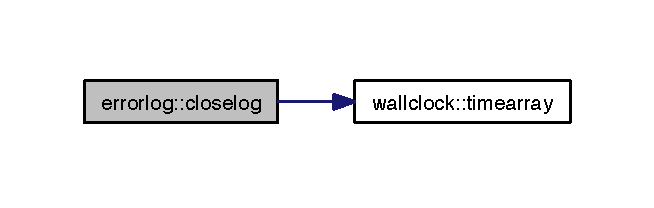
\includegraphics[width=311pt]{classerrorlog_af9219c790b58905faca7f5695515325d_cgraph}
\end{center}
\end{figure}




Here is the caller graph for this function\+:\nopagebreak
\begin{figure}[H]
\begin{center}
\leavevmode
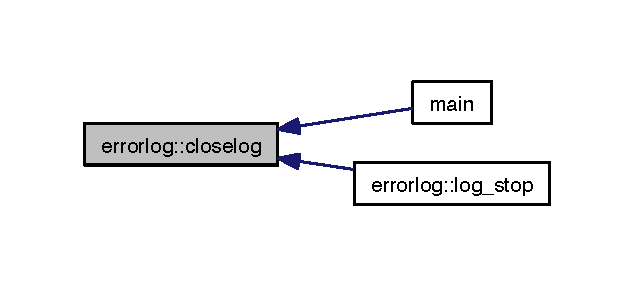
\includegraphics[width=299pt]{classerrorlog_af9219c790b58905faca7f5695515325d_icgraph}
\end{center}
\end{figure}


\hypertarget{classerrorlog_a05d233f410ba88bf3e2929528b1bb91e}{\index{errorlog@{errorlog}!displaylog@{displaylog}}
\index{displaylog@{displaylog}!errorlog@{errorlog}}
\subsubsection[{displaylog}]{\setlength{\rightskip}{0pt plus 5cm}subroutine, public errorlog\+::displaylog (
\begin{DoxyParamCaption}
{}
\end{DoxyParamCaption}
)}}\label{classerrorlog_a05d233f410ba88bf3e2929528b1bb91e}
\hypertarget{classerrorlog_abcaf87ab55e0634007cc7177aa53469c}{\index{errorlog@{errorlog}!log\+\_\+note@{log\+\_\+note}}
\index{log\+\_\+note@{log\+\_\+note}!errorlog@{errorlog}}
\subsubsection[{log\+\_\+note}]{\setlength{\rightskip}{0pt plus 5cm}subroutine errorlog\+::log\+\_\+note (
\begin{DoxyParamCaption}
\item[{character$\ast$($\ast$), intent(in)}]{msg}
\end{DoxyParamCaption}
)\hspace{0.3cm}{\ttfamily [private]}}}\label{classerrorlog_abcaf87ab55e0634007cc7177aa53469c}


Here is the call graph for this function\+:\nopagebreak
\begin{figure}[H]
\begin{center}
\leavevmode
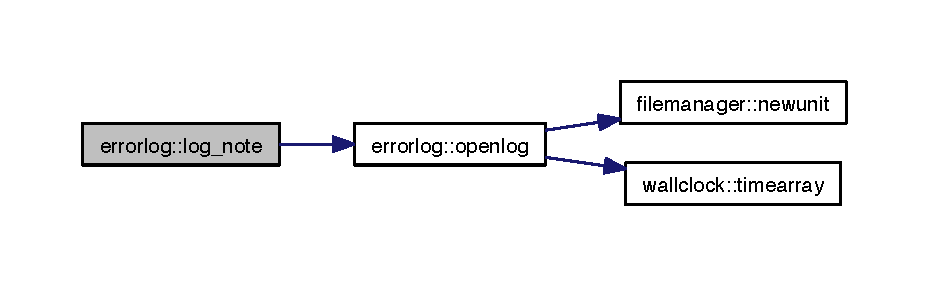
\includegraphics[width=350pt]{classerrorlog_abcaf87ab55e0634007cc7177aa53469c_cgraph}
\end{center}
\end{figure}


\hypertarget{classerrorlog_ac6531d63b5a5d4939c3d510dd7fbbb25}{\index{errorlog@{errorlog}!log\+\_\+prompt@{log\+\_\+prompt}}
\index{log\+\_\+prompt@{log\+\_\+prompt}!errorlog@{errorlog}}
\subsubsection[{log\+\_\+prompt}]{\setlength{\rightskip}{0pt plus 5cm}subroutine errorlog\+::log\+\_\+prompt (
\begin{DoxyParamCaption}
\item[{character$\ast$($\ast$), intent(in)}]{msg}
\end{DoxyParamCaption}
)\hspace{0.3cm}{\ttfamily [private]}}}\label{classerrorlog_ac6531d63b5a5d4939c3d510dd7fbbb25}


Here is the call graph for this function\+:\nopagebreak
\begin{figure}[H]
\begin{center}
\leavevmode
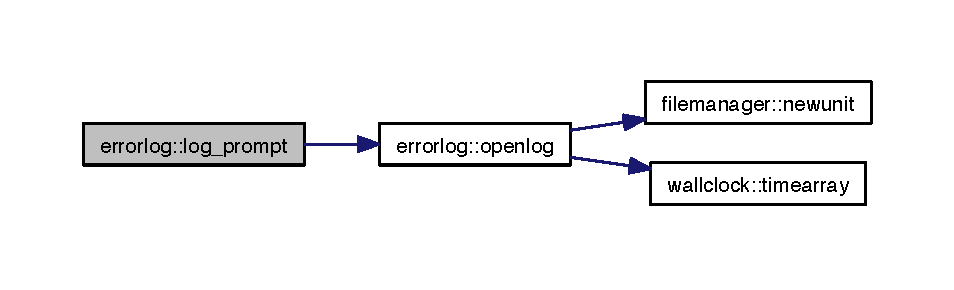
\includegraphics[width=350pt]{classerrorlog_ac6531d63b5a5d4939c3d510dd7fbbb25_cgraph}
\end{center}
\end{figure}


\hypertarget{classerrorlog_afe1872ea4ca114ccb25faaa2f2d60e2e}{\index{errorlog@{errorlog}!log\+\_\+stop@{log\+\_\+stop}}
\index{log\+\_\+stop@{log\+\_\+stop}!errorlog@{errorlog}}
\subsubsection[{log\+\_\+stop}]{\setlength{\rightskip}{0pt plus 5cm}subroutine errorlog\+::log\+\_\+stop (
\begin{DoxyParamCaption}
\item[{character$\ast$($\ast$), intent(in)}]{msg, }
\item[{character$\ast$($\ast$), intent(in), optional}]{suggest}
\end{DoxyParamCaption}
)\hspace{0.3cm}{\ttfamily [private]}}}\label{classerrorlog_afe1872ea4ca114ccb25faaa2f2d60e2e}


Here is the call graph for this function\+:\nopagebreak
\begin{figure}[H]
\begin{center}
\leavevmode
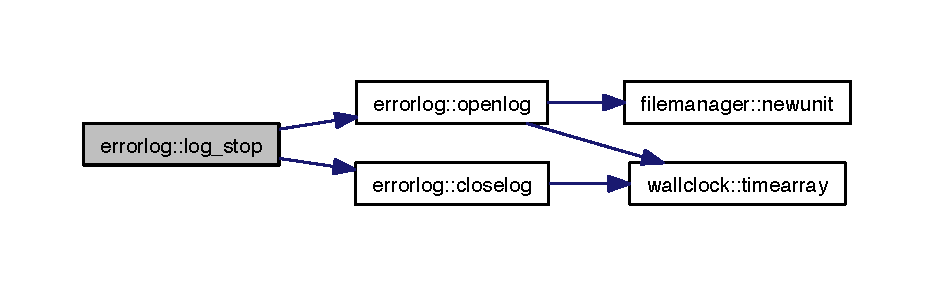
\includegraphics[width=350pt]{classerrorlog_afe1872ea4ca114ccb25faaa2f2d60e2e_cgraph}
\end{center}
\end{figure}


\hypertarget{classerrorlog_ac0a3d2c2bcdb3af8e91b4a27d2ac5ac0}{\index{errorlog@{errorlog}!log\+\_\+warn@{log\+\_\+warn}}
\index{log\+\_\+warn@{log\+\_\+warn}!errorlog@{errorlog}}
\subsubsection[{log\+\_\+warn}]{\setlength{\rightskip}{0pt plus 5cm}subroutine errorlog\+::log\+\_\+warn (
\begin{DoxyParamCaption}
\item[{character$\ast$($\ast$), intent(in)}]{msg, }
\item[{character$\ast$($\ast$), intent(in), optional}]{recover}
\end{DoxyParamCaption}
)\hspace{0.3cm}{\ttfamily [private]}}}\label{classerrorlog_ac0a3d2c2bcdb3af8e91b4a27d2ac5ac0}


Here is the call graph for this function\+:\nopagebreak
\begin{figure}[H]
\begin{center}
\leavevmode
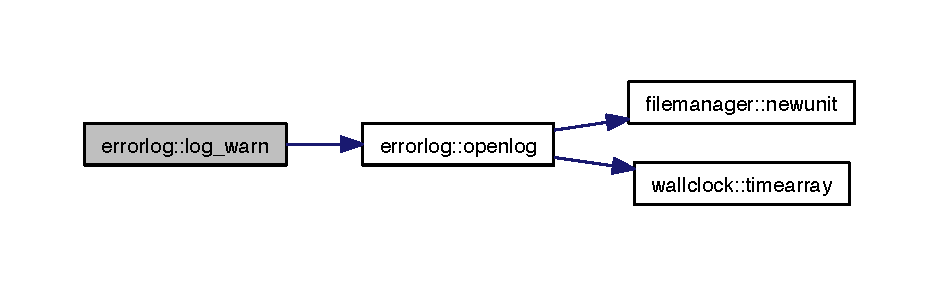
\includegraphics[width=350pt]{classerrorlog_ac0a3d2c2bcdb3af8e91b4a27d2ac5ac0_cgraph}
\end{center}
\end{figure}


\hypertarget{classerrorlog_a32bbf87dd265de25bd10ea31d95b751d}{\index{errorlog@{errorlog}!openlog@{openlog}}
\index{openlog@{openlog}!errorlog@{errorlog}}
\subsubsection[{openlog}]{\setlength{\rightskip}{0pt plus 5cm}subroutine, public errorlog\+::openlog (
\begin{DoxyParamCaption}
\item[{character$\ast$($\ast$), intent(in), optional}]{file, }
\item[{integer(short), intent(in), optional}]{level, }
\item[{character$\ast$($\ast$), intent(in), optional}]{Program\+Name, }
\item[{character$\ast$($\ast$), intent(in), optional}]{Bug\+Report}
\end{DoxyParamCaption}
)}}\label{classerrorlog_a32bbf87dd265de25bd10ea31d95b751d}


Here is the call graph for this function\+:\nopagebreak
\begin{figure}[H]
\begin{center}
\leavevmode
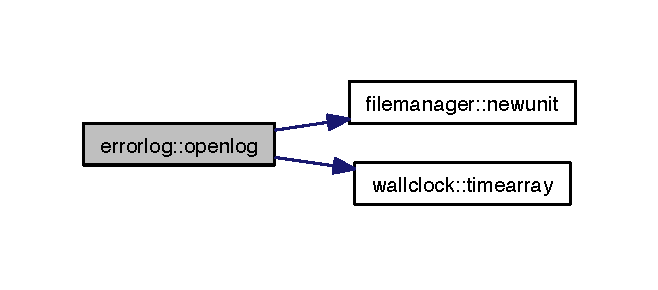
\includegraphics[width=312pt]{classerrorlog_a32bbf87dd265de25bd10ea31d95b751d_cgraph}
\end{center}
\end{figure}




Here is the caller graph for this function\+:\nopagebreak
\begin{figure}[H]
\begin{center}
\leavevmode
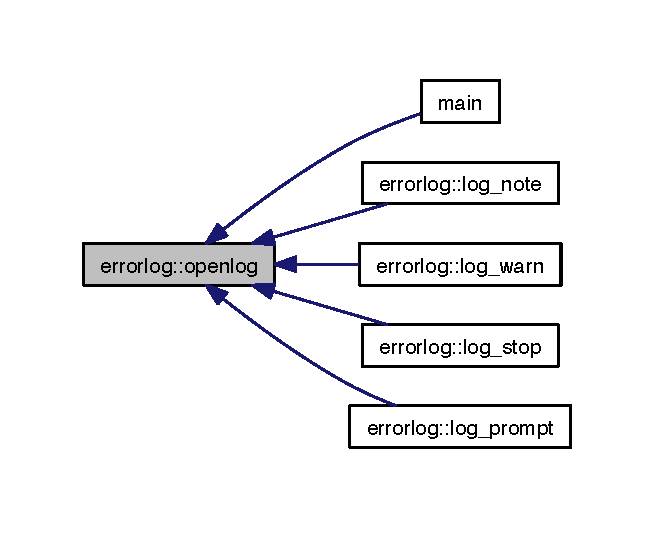
\includegraphics[width=308pt]{classerrorlog_a32bbf87dd265de25bd10ea31d95b751d_icgraph}
\end{center}
\end{figure}




\subsection{Member Data Documentation}
\hypertarget{classerrorlog_af9add736038cc71b13ee19df6544f3e5}{\index{errorlog@{errorlog}!logclosed@{logclosed}}
\index{logclosed@{logclosed}!errorlog@{errorlog}}
\subsubsection[{logclosed}]{\setlength{\rightskip}{0pt plus 5cm}logical errorlog\+::logclosed\hspace{0.3cm}{\ttfamily [private]}}}\label{classerrorlog_af9add736038cc71b13ee19df6544f3e5}
\hypertarget{classerrorlog_a056ccc9457985050fb6391dd4abf1f2c}{\index{errorlog@{errorlog}!logcount@{logcount}}
\index{logcount@{logcount}!errorlog@{errorlog}}
\subsubsection[{logcount}]{\setlength{\rightskip}{0pt plus 5cm}integer(long) errorlog\+::logcount\hspace{0.3cm}{\ttfamily [private]}}}\label{classerrorlog_a056ccc9457985050fb6391dd4abf1f2c}
\hypertarget{classerrorlog_a42e82497abf38d3e1683b51b48a5e4c0}{\index{errorlog@{errorlog}!logfile@{logfile}}
\index{logfile@{logfile}!errorlog@{errorlog}}
\subsubsection[{logfile}]{\setlength{\rightskip}{0pt plus 5cm}character(len=path) errorlog\+::logfile\hspace{0.3cm}{\ttfamily [private]}}}\label{classerrorlog_a42e82497abf38d3e1683b51b48a5e4c0}
\hypertarget{classerrorlog_a3ab7fc512e499660dcb9a9542aab02b5}{\index{errorlog@{errorlog}!loglevel@{loglevel}}
\index{loglevel@{loglevel}!errorlog@{errorlog}}
\subsubsection[{loglevel}]{\setlength{\rightskip}{0pt plus 5cm}integer(short) errorlog\+::loglevel\hspace{0.3cm}{\ttfamily [private]}}}\label{classerrorlog_a3ab7fc512e499660dcb9a9542aab02b5}
\hypertarget{classerrorlog_a3a12f9c3cbb079a8cbb7b5790ea2c827}{\index{errorlog@{errorlog}!logopen@{logopen}}
\index{logopen@{logopen}!errorlog@{errorlog}}
\subsubsection[{logopen}]{\setlength{\rightskip}{0pt plus 5cm}logical errorlog\+::logopen\hspace{0.3cm}{\ttfamily [private]}}}\label{classerrorlog_a3a12f9c3cbb079a8cbb7b5790ea2c827}
\hypertarget{classerrorlog_adb26bb2d10f764e895c9745c3fb5dd1d}{\index{errorlog@{errorlog}!logunit@{logunit}}
\index{logunit@{logunit}!errorlog@{errorlog}}
\subsubsection[{logunit}]{\setlength{\rightskip}{0pt plus 5cm}integer(long) errorlog\+::logunit\hspace{0.3cm}{\ttfamily [private]}}}\label{classerrorlog_adb26bb2d10f764e895c9745c3fb5dd1d}


The documentation for this module was generated from the following file\+:\begin{DoxyCompactItemize}
\item 
src/\hyperlink{utils_8f90}{utils.\+f90}\end{DoxyCompactItemize}

\hypertarget{classfilemanager}{\section{filemanager Module Reference}
\label{classfilemanager}\index{filemanager@{filemanager}}
}
\subsection*{Data Types}
\begin{DoxyCompactItemize}
\item 
interface \hyperlink{interfacefilemanager_1_1check}{check}
\end{DoxyCompactItemize}
\subsection*{Public Member Functions}
\begin{DoxyCompactItemize}
\item 
integer(long) function, public \hyperlink{classfilemanager_aa389048ef7c9eb9afdac7ce1dcc691b2}{newunit} ()
\end{DoxyCompactItemize}
\subsection*{Private Member Functions}
\begin{DoxyCompactItemize}
\item 
integer(short) function \hyperlink{classfilemanager_a0c7a869ddf6cd3ea9fad5b6de4069cf3}{checkfile} (file)
\end{DoxyCompactItemize}


\subsection{Member Function/\+Subroutine Documentation}
\hypertarget{classfilemanager_a0c7a869ddf6cd3ea9fad5b6de4069cf3}{\index{filemanager@{filemanager}!checkfile@{checkfile}}
\index{checkfile@{checkfile}!filemanager@{filemanager}}
\subsubsection[{checkfile}]{\setlength{\rightskip}{0pt plus 5cm}integer(short) function filemanager\+::checkfile (
\begin{DoxyParamCaption}
\item[{character$\ast$($\ast$), intent(in)}]{file}
\end{DoxyParamCaption}
)\hspace{0.3cm}{\ttfamily [private]}}}\label{classfilemanager_a0c7a869ddf6cd3ea9fad5b6de4069cf3}


Here is the call graph for this function\+:\nopagebreak
\begin{figure}[H]
\begin{center}
\leavevmode
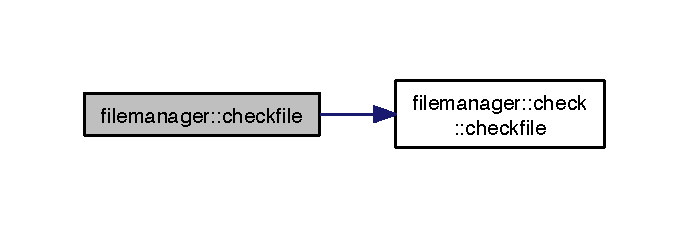
\includegraphics[width=327pt]{classfilemanager_a0c7a869ddf6cd3ea9fad5b6de4069cf3_cgraph}
\end{center}
\end{figure}


\hypertarget{classfilemanager_aa389048ef7c9eb9afdac7ce1dcc691b2}{\index{filemanager@{filemanager}!newunit@{newunit}}
\index{newunit@{newunit}!filemanager@{filemanager}}
\subsubsection[{newunit}]{\setlength{\rightskip}{0pt plus 5cm}integer(long) function, public filemanager\+::newunit (
\begin{DoxyParamCaption}
{}
\end{DoxyParamCaption}
)}}\label{classfilemanager_aa389048ef7c9eb9afdac7ce1dcc691b2}


Here is the caller graph for this function\+:\nopagebreak
\begin{figure}[H]
\begin{center}
\leavevmode
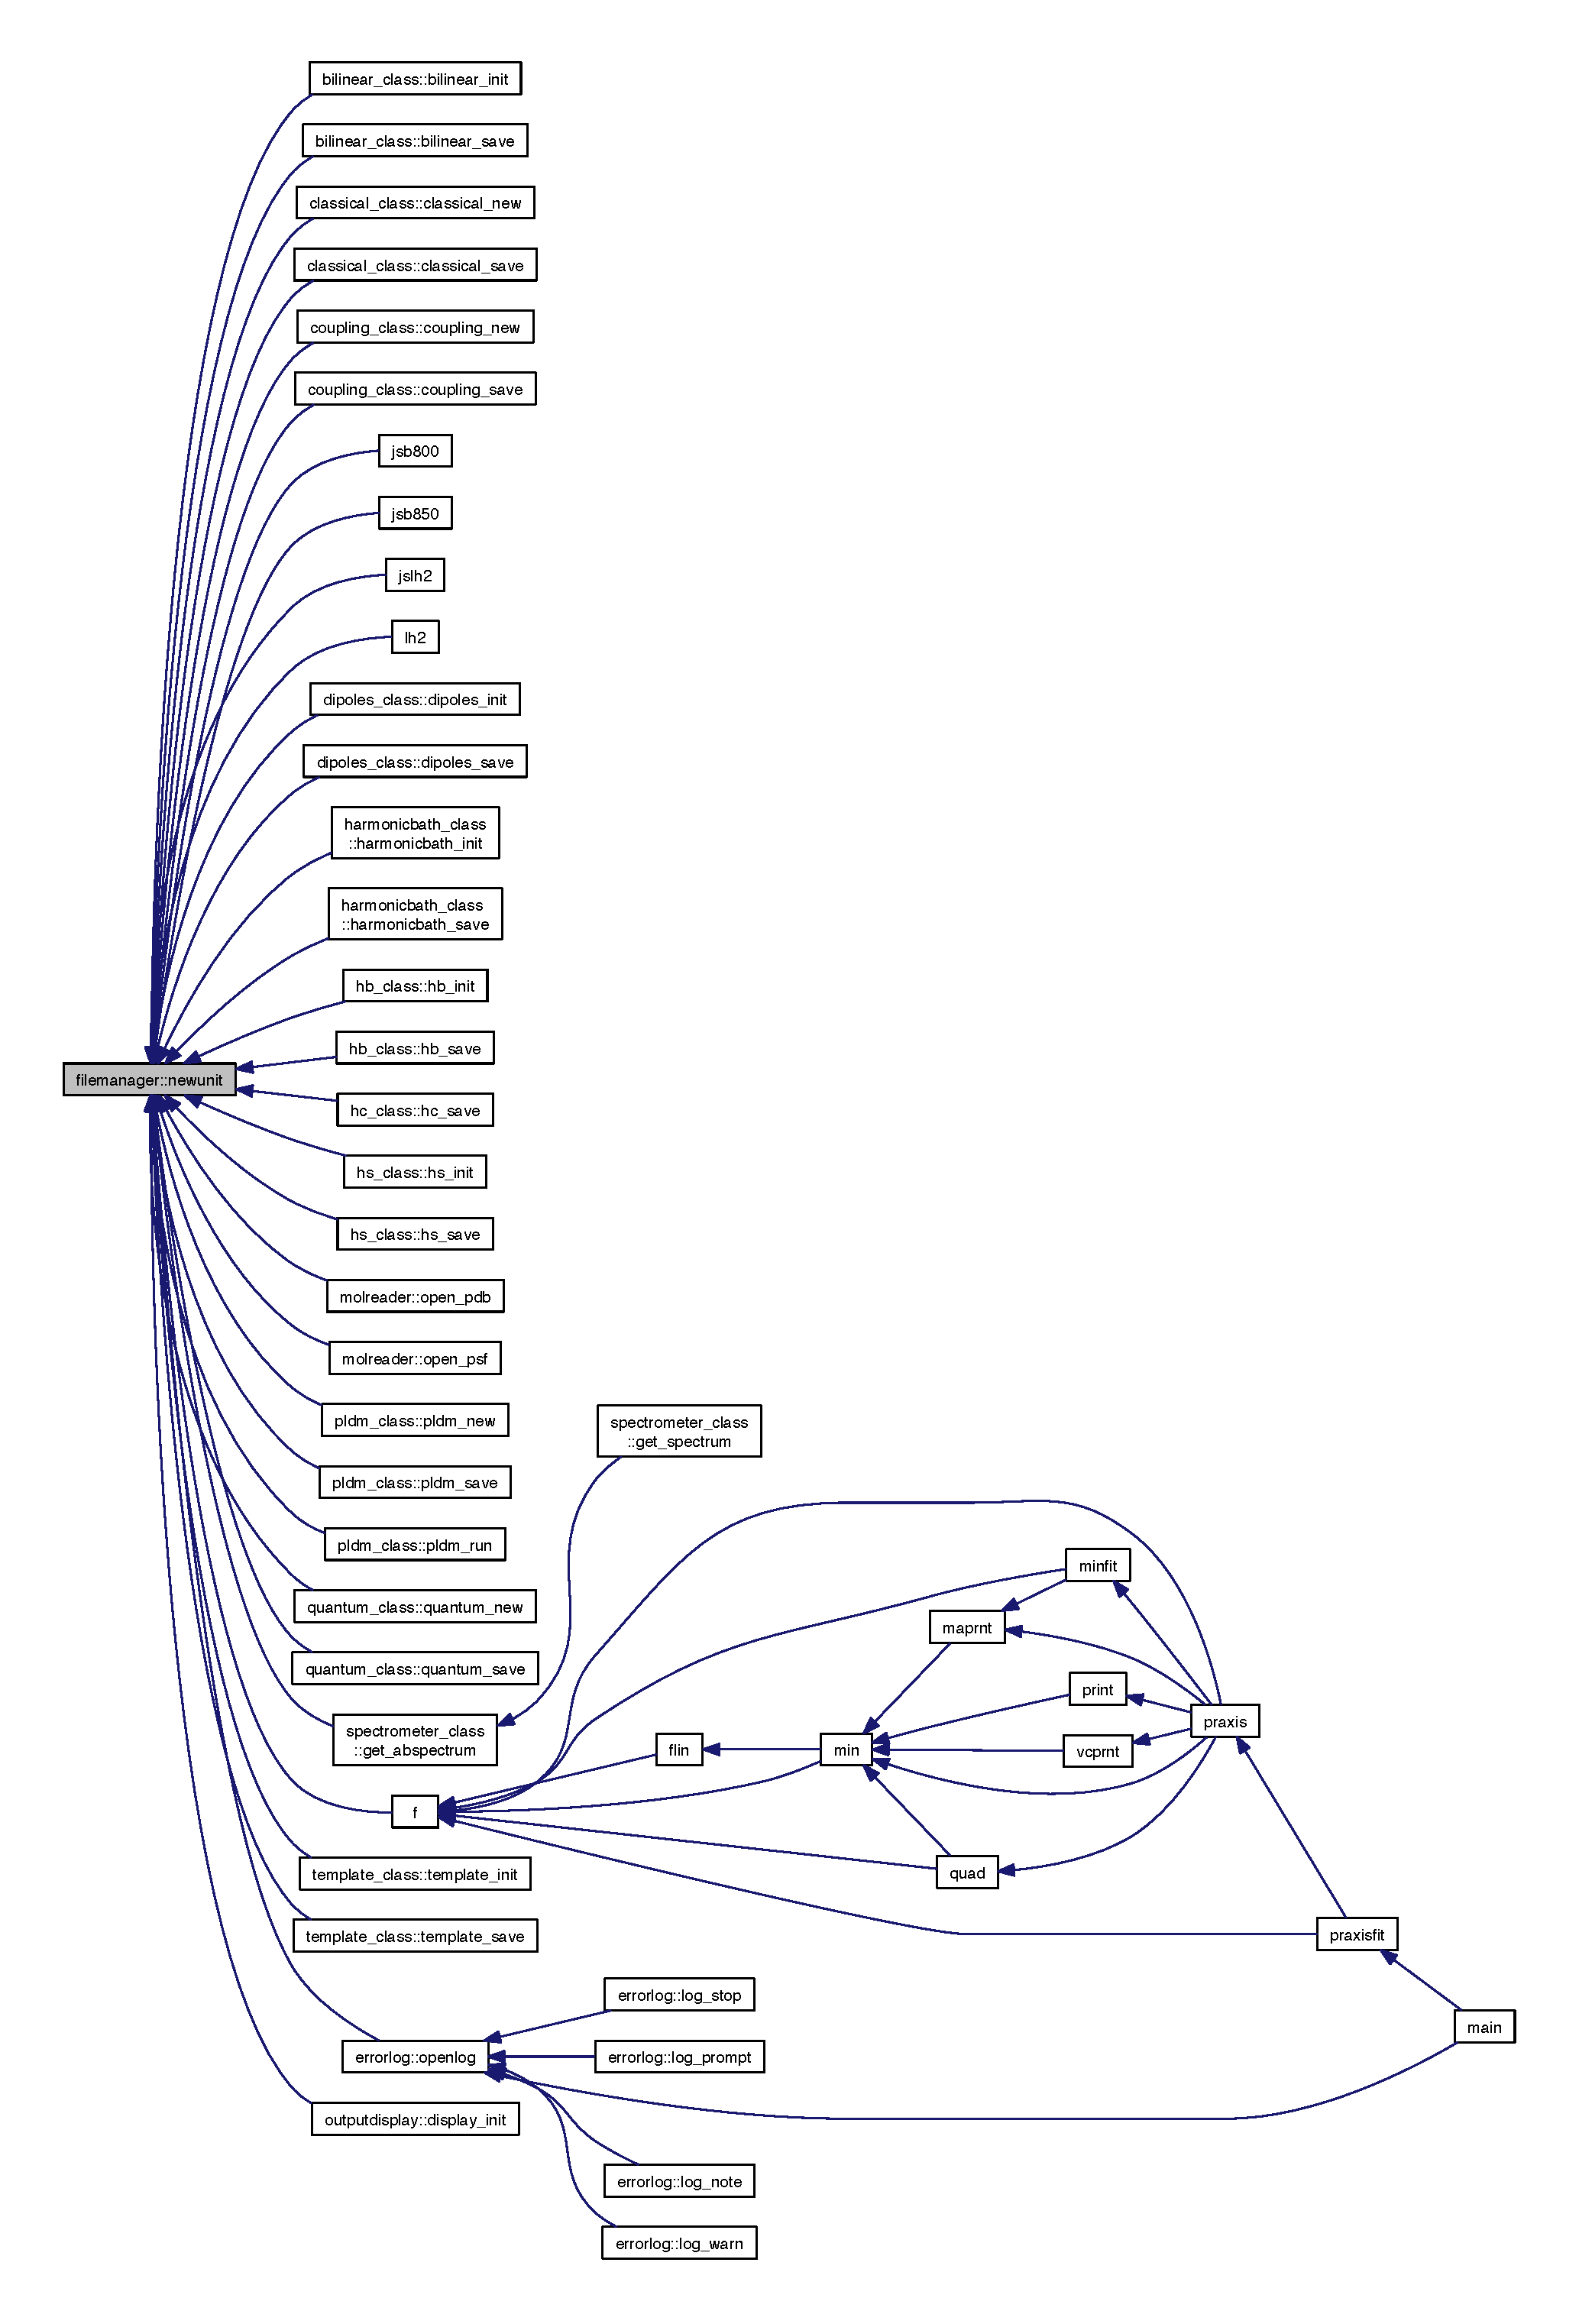
\includegraphics[height=550pt]{classfilemanager_aa389048ef7c9eb9afdac7ce1dcc691b2_icgraph}
\end{center}
\end{figure}




The documentation for this module was generated from the following file\+:\begin{DoxyCompactItemize}
\item 
src/\hyperlink{utils_8f90}{utils.\+f90}\end{DoxyCompactItemize}

\hypertarget{interfacefitxydata_1_1fit2exp}{\section{fitxydata\+:\+:fit2exp Interface Reference}
\label{interfacefitxydata_1_1fit2exp}\index{fitxydata\+::fit2exp@{fitxydata\+::fit2exp}}
}
\subsection*{Private Member Functions}
\begin{DoxyCompactItemize}
\item 
subroutine \hyperlink{interfacefitxydata_1_1fit2exp_a73b64486284b328876b36875d2006a98}{fit2exp} (set, R, A, B)
\begin{DoxyCompactList}\small\item\em Fit to exponential function. \end{DoxyCompactList}\end{DoxyCompactItemize}


\subsection{Constructor \& Destructor Documentation}
\hypertarget{interfacefitxydata_1_1fit2exp_a73b64486284b328876b36875d2006a98}{\index{fitxydata\+::fit2exp@{fitxydata\+::fit2exp}!fit2exp@{fit2exp}}
\index{fit2exp@{fit2exp}!fitxydata\+::fit2exp@{fitxydata\+::fit2exp}}
\subsubsection[{fit2exp}]{\setlength{\rightskip}{0pt plus 5cm}subroutine fitxydata\+::fit2exp\+::fit2exp (
\begin{DoxyParamCaption}
\item[{real$\ast$8, dimension(\+:,\+:), intent(in)}]{set, }
\item[{real$\ast$8, intent(inout)}]{R, }
\item[{real$\ast$8, intent(inout)}]{A, }
\item[{real$\ast$8, intent(inout), optional}]{B}
\end{DoxyParamCaption}
)\hspace{0.3cm}{\ttfamily [private]}}}\label{interfacefitxydata_1_1fit2exp_a73b64486284b328876b36875d2006a98}


Fit to exponential function. 

fits set to exp function (A-\/\+B)$\ast$exp(-\/\+R$\ast$t)+\+B 

The documentation for this interface was generated from the following file\+:\begin{DoxyCompactItemize}
\item 
src/\hyperlink{utils_8f90}{utils.\+f90}\end{DoxyCompactItemize}

\hypertarget{classfitxydata}{\section{fitxydata Module Reference}
\label{classfitxydata}\index{fitxydata@{fitxydata}}
}


Procedures to Fit X\-Y data to functional forms.  


\subsection*{Data Types}
\begin{DoxyCompactItemize}
\item 
interface \hyperlink{interfacefitxydata_1_1fit2exp}{fit2exp}
\end{DoxyCompactItemize}
\subsection*{Public Member Functions}
\begin{DoxyCompactItemize}
\item 
subroutine, public \hyperlink{classfitxydata_a9f00dca017c2372da0c3c95cdf0ddb31}{fit2exp} (set, R, A, B)
\begin{DoxyCompactList}\small\item\em Fit to exponential function. \end{DoxyCompactList}\end{DoxyCompactItemize}
\subsection*{Private Attributes}
\begin{DoxyCompactItemize}
\item 
real $\ast$8, dimension(\-:,\-:), \\*
allocatable \hyperlink{classfitxydata_ad69a6716eab16a1f8c170a0d0a7ed499}{xydata}
\end{DoxyCompactItemize}


\subsection{Detailed Description}
Procedures to Fit X\-Y data to functional forms. 

Returns select function parameters 

\subsection{Member Function/\-Subroutine Documentation}
\hypertarget{classfitxydata_a9f00dca017c2372da0c3c95cdf0ddb31}{\index{fitxydata@{fitxydata}!fit2exp@{fit2exp}}
\index{fit2exp@{fit2exp}!fitxydata@{fitxydata}}
\subsubsection[{fit2exp}]{\setlength{\rightskip}{0pt plus 5cm}subroutine, public {\bf fitxydata\-::fit2exp} (
\begin{DoxyParamCaption}
\item[{real$\ast$8, dimension(\-:,\-:), intent(in)}]{set, }
\item[{real$\ast$8, intent(inout)}]{R, }
\item[{real$\ast$8, intent(inout)}]{A, }
\item[{real$\ast$8, intent(inout), optional}]{B}
\end{DoxyParamCaption}
)}}\label{classfitxydata_a9f00dca017c2372da0c3c95cdf0ddb31}


Fit to exponential function. 

fits set to exp function (A-\/\-B)$\ast$exp(-\/\-R$\ast$t)+\-B 

\subsection{Member Data Documentation}
\hypertarget{classfitxydata_ad69a6716eab16a1f8c170a0d0a7ed499}{\index{fitxydata@{fitxydata}!xydata@{xydata}}
\index{xydata@{xydata}!fitxydata@{fitxydata}}
\subsubsection[{xydata}]{\setlength{\rightskip}{0pt plus 5cm}real$\ast$8, dimension(\-:,\-:), allocatable fitxydata\-::xydata\hspace{0.3cm}{\ttfamily [private]}}}\label{classfitxydata_ad69a6716eab16a1f8c170a0d0a7ed499}


The documentation for this module was generated from the following file\-:\begin{DoxyCompactItemize}
\item 
src/\hyperlink{utils_8f90}{utils.\-f90}\end{DoxyCompactItemize}

\hypertarget{interfacestring_1_1float2str}{}\section{string\+:\+:float2str Interface Reference}
\label{interfacestring_1_1float2str}\index{string\+::float2str@{string\+::float2str}}
\subsection*{Private Member Functions}
\begin{DoxyCompactItemize}
\item 
character(len=title) function \hyperlink{interfacestring_1_1float2str_a2fcaf4fe5a7a6482089bcdb7ef00d16e}{double2str} (X)
\item 
character(len=title) function \hyperlink{interfacestring_1_1float2str_afd5dc692bff7633a54d493dcc93df16f}{single2str} (X)
\end{DoxyCompactItemize}


\subsection{Member Function/\+Subroutine Documentation}
\mbox{\Hypertarget{interfacestring_1_1float2str_a2fcaf4fe5a7a6482089bcdb7ef00d16e}\label{interfacestring_1_1float2str_a2fcaf4fe5a7a6482089bcdb7ef00d16e}} 
\index{string\+::float2str@{string\+::float2str}!double2str@{double2str}}
\index{double2str@{double2str}!string\+::float2str@{string\+::float2str}}
\subsubsection{\texorpdfstring{double2str()}{double2str()}}
{\footnotesize\ttfamily character(len=title) function string\+::float2str\+::double2str (\begin{DoxyParamCaption}\item[{real(double), intent(in)}]{X }\end{DoxyParamCaption})\hspace{0.3cm}{\ttfamily [private]}}

\mbox{\Hypertarget{interfacestring_1_1float2str_afd5dc692bff7633a54d493dcc93df16f}\label{interfacestring_1_1float2str_afd5dc692bff7633a54d493dcc93df16f}} 
\index{string\+::float2str@{string\+::float2str}!single2str@{single2str}}
\index{single2str@{single2str}!string\+::float2str@{string\+::float2str}}
\subsubsection{\texorpdfstring{single2str()}{single2str()}}
{\footnotesize\ttfamily character(len=title) function string\+::float2str\+::single2str (\begin{DoxyParamCaption}\item[{real(single), intent(in)}]{X }\end{DoxyParamCaption})\hspace{0.3cm}{\ttfamily [private]}}



The documentation for this interface was generated from the following file\+:\begin{DoxyCompactItemize}
\item 
src/\hyperlink{utils_8f90}{utils.\+f90}\end{DoxyCompactItemize}

\hypertarget{structharmonicbath__class_1_1harmonicbath}{}\section{harmonicbath\+\_\+class\+:\+:harmonicbath Type Reference}
\label{structharmonicbath__class_1_1harmonicbath}\index{harmonicbath\+\_\+class\+::harmonicbath@{harmonicbath\+\_\+class\+::harmonicbath}}


Collaboration diagram for harmonicbath\+\_\+class\+:\+:harmonicbath\+:\nopagebreak
\begin{figure}[H]
\begin{center}
\leavevmode
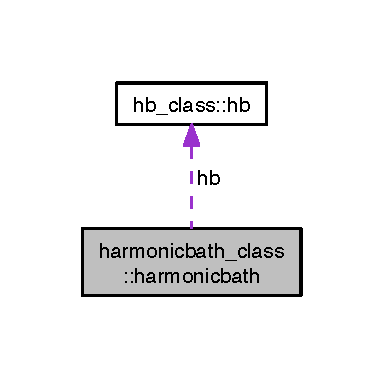
\includegraphics[width=184pt]{structharmonicbath__class_1_1harmonicbath__coll__graph}
\end{center}
\end{figure}
\subsection*{Private Attributes}
\begin{DoxyCompactItemize}
\item 
logical \hyperlink{structharmonicbath__class_1_1harmonicbath_a876fbdf98da8f3bfeb4b4e03b58d6f74}{initialized}
\item 
type(\hyperlink{structhb__class_1_1hb}{hb}) \hyperlink{structharmonicbath__class_1_1harmonicbath_a7b59e71a4b2100f821d091a5193d50f5}{hb}
\item 
integer(long) \hyperlink{structharmonicbath__class_1_1harmonicbath_ad55e02fae968c36f82bcfa4faf61d978}{nbath}
\item 
integer(long) \hyperlink{structharmonicbath__class_1_1harmonicbath_ab292a58613813f3ee812f949f9899089}{npt}
\item 
integer(long) \hyperlink{structharmonicbath__class_1_1harmonicbath_a87afd4834fce3bda38f7c49ecb203121}{nden}
\item 
real(double), dimension(\+:), pointer \hyperlink{structharmonicbath__class_1_1harmonicbath_a4268e843792e21ac9c78224a9e540e1f}{wgrid}
\item 
real(double), dimension(\+:,\+:), pointer \hyperlink{structharmonicbath__class_1_1harmonicbath_a5d4365532fe5feb53eb8bf06a64c8bcc}{jw}
\item 
real(double), dimension(\+:,\+:), pointer \hyperlink{structharmonicbath__class_1_1harmonicbath_aded5880e44b831dddae5be30966594e4}{intdos}
\item 
real(double), dimension(\+:), pointer \hyperlink{structharmonicbath__class_1_1harmonicbath_abdcf7e97525bd1bd424af202df2c5253}{lambda}
\item 
integer(long), dimension(\+:), pointer \hyperlink{structharmonicbath__class_1_1harmonicbath_a080d6ce6fdb6481bb8851b4fbc24a995}{map}
\item 
logical \hyperlink{structharmonicbath__class_1_1harmonicbath_a1ae24e6ddcc5e0a0b80decc16a0865cb}{stochasticsample}
\end{DoxyCompactItemize}


\subsection{Member Data Documentation}
\mbox{\Hypertarget{structharmonicbath__class_1_1harmonicbath_a7b59e71a4b2100f821d091a5193d50f5}\label{structharmonicbath__class_1_1harmonicbath_a7b59e71a4b2100f821d091a5193d50f5}} 
\index{harmonicbath\+\_\+class\+::harmonicbath@{harmonicbath\+\_\+class\+::harmonicbath}!hb@{hb}}
\index{hb@{hb}!harmonicbath\+\_\+class\+::harmonicbath@{harmonicbath\+\_\+class\+::harmonicbath}}
\subsubsection{\texorpdfstring{hb}{hb}}
{\footnotesize\ttfamily type(\hyperlink{structhb__class_1_1hb}{hb}) harmonicbath\+\_\+class\+::harmonicbath\+::hb\hspace{0.3cm}{\ttfamily [private]}}

\mbox{\Hypertarget{structharmonicbath__class_1_1harmonicbath_a876fbdf98da8f3bfeb4b4e03b58d6f74}\label{structharmonicbath__class_1_1harmonicbath_a876fbdf98da8f3bfeb4b4e03b58d6f74}} 
\index{harmonicbath\+\_\+class\+::harmonicbath@{harmonicbath\+\_\+class\+::harmonicbath}!initialized@{initialized}}
\index{initialized@{initialized}!harmonicbath\+\_\+class\+::harmonicbath@{harmonicbath\+\_\+class\+::harmonicbath}}
\subsubsection{\texorpdfstring{initialized}{initialized}}
{\footnotesize\ttfamily logical harmonicbath\+\_\+class\+::harmonicbath\+::initialized\hspace{0.3cm}{\ttfamily [private]}}

\mbox{\Hypertarget{structharmonicbath__class_1_1harmonicbath_aded5880e44b831dddae5be30966594e4}\label{structharmonicbath__class_1_1harmonicbath_aded5880e44b831dddae5be30966594e4}} 
\index{harmonicbath\+\_\+class\+::harmonicbath@{harmonicbath\+\_\+class\+::harmonicbath}!intdos@{intdos}}
\index{intdos@{intdos}!harmonicbath\+\_\+class\+::harmonicbath@{harmonicbath\+\_\+class\+::harmonicbath}}
\subsubsection{\texorpdfstring{intdos}{intdos}}
{\footnotesize\ttfamily real(double), dimension(\+:,\+:), pointer harmonicbath\+\_\+class\+::harmonicbath\+::intdos\hspace{0.3cm}{\ttfamily [private]}}

\mbox{\Hypertarget{structharmonicbath__class_1_1harmonicbath_a5d4365532fe5feb53eb8bf06a64c8bcc}\label{structharmonicbath__class_1_1harmonicbath_a5d4365532fe5feb53eb8bf06a64c8bcc}} 
\index{harmonicbath\+\_\+class\+::harmonicbath@{harmonicbath\+\_\+class\+::harmonicbath}!jw@{jw}}
\index{jw@{jw}!harmonicbath\+\_\+class\+::harmonicbath@{harmonicbath\+\_\+class\+::harmonicbath}}
\subsubsection{\texorpdfstring{jw}{jw}}
{\footnotesize\ttfamily real(double), dimension(\+:,\+:), pointer harmonicbath\+\_\+class\+::harmonicbath\+::jw\hspace{0.3cm}{\ttfamily [private]}}

\mbox{\Hypertarget{structharmonicbath__class_1_1harmonicbath_abdcf7e97525bd1bd424af202df2c5253}\label{structharmonicbath__class_1_1harmonicbath_abdcf7e97525bd1bd424af202df2c5253}} 
\index{harmonicbath\+\_\+class\+::harmonicbath@{harmonicbath\+\_\+class\+::harmonicbath}!lambda@{lambda}}
\index{lambda@{lambda}!harmonicbath\+\_\+class\+::harmonicbath@{harmonicbath\+\_\+class\+::harmonicbath}}
\subsubsection{\texorpdfstring{lambda}{lambda}}
{\footnotesize\ttfamily real(double), dimension(\+:), pointer harmonicbath\+\_\+class\+::harmonicbath\+::lambda\hspace{0.3cm}{\ttfamily [private]}}

\mbox{\Hypertarget{structharmonicbath__class_1_1harmonicbath_a080d6ce6fdb6481bb8851b4fbc24a995}\label{structharmonicbath__class_1_1harmonicbath_a080d6ce6fdb6481bb8851b4fbc24a995}} 
\index{harmonicbath\+\_\+class\+::harmonicbath@{harmonicbath\+\_\+class\+::harmonicbath}!map@{map}}
\index{map@{map}!harmonicbath\+\_\+class\+::harmonicbath@{harmonicbath\+\_\+class\+::harmonicbath}}
\subsubsection{\texorpdfstring{map}{map}}
{\footnotesize\ttfamily integer(long), dimension(\+:), pointer harmonicbath\+\_\+class\+::harmonicbath\+::map\hspace{0.3cm}{\ttfamily [private]}}

\mbox{\Hypertarget{structharmonicbath__class_1_1harmonicbath_ad55e02fae968c36f82bcfa4faf61d978}\label{structharmonicbath__class_1_1harmonicbath_ad55e02fae968c36f82bcfa4faf61d978}} 
\index{harmonicbath\+\_\+class\+::harmonicbath@{harmonicbath\+\_\+class\+::harmonicbath}!nbath@{nbath}}
\index{nbath@{nbath}!harmonicbath\+\_\+class\+::harmonicbath@{harmonicbath\+\_\+class\+::harmonicbath}}
\subsubsection{\texorpdfstring{nbath}{nbath}}
{\footnotesize\ttfamily integer(long) harmonicbath\+\_\+class\+::harmonicbath\+::nbath\hspace{0.3cm}{\ttfamily [private]}}

\mbox{\Hypertarget{structharmonicbath__class_1_1harmonicbath_a87afd4834fce3bda38f7c49ecb203121}\label{structharmonicbath__class_1_1harmonicbath_a87afd4834fce3bda38f7c49ecb203121}} 
\index{harmonicbath\+\_\+class\+::harmonicbath@{harmonicbath\+\_\+class\+::harmonicbath}!nden@{nden}}
\index{nden@{nden}!harmonicbath\+\_\+class\+::harmonicbath@{harmonicbath\+\_\+class\+::harmonicbath}}
\subsubsection{\texorpdfstring{nden}{nden}}
{\footnotesize\ttfamily integer(long) harmonicbath\+\_\+class\+::harmonicbath\+::nden\hspace{0.3cm}{\ttfamily [private]}}

\mbox{\Hypertarget{structharmonicbath__class_1_1harmonicbath_ab292a58613813f3ee812f949f9899089}\label{structharmonicbath__class_1_1harmonicbath_ab292a58613813f3ee812f949f9899089}} 
\index{harmonicbath\+\_\+class\+::harmonicbath@{harmonicbath\+\_\+class\+::harmonicbath}!npt@{npt}}
\index{npt@{npt}!harmonicbath\+\_\+class\+::harmonicbath@{harmonicbath\+\_\+class\+::harmonicbath}}
\subsubsection{\texorpdfstring{npt}{npt}}
{\footnotesize\ttfamily integer(long) harmonicbath\+\_\+class\+::harmonicbath\+::npt\hspace{0.3cm}{\ttfamily [private]}}

\mbox{\Hypertarget{structharmonicbath__class_1_1harmonicbath_a1ae24e6ddcc5e0a0b80decc16a0865cb}\label{structharmonicbath__class_1_1harmonicbath_a1ae24e6ddcc5e0a0b80decc16a0865cb}} 
\index{harmonicbath\+\_\+class\+::harmonicbath@{harmonicbath\+\_\+class\+::harmonicbath}!stochasticsample@{stochasticsample}}
\index{stochasticsample@{stochasticsample}!harmonicbath\+\_\+class\+::harmonicbath@{harmonicbath\+\_\+class\+::harmonicbath}}
\subsubsection{\texorpdfstring{stochasticsample}{stochasticsample}}
{\footnotesize\ttfamily logical harmonicbath\+\_\+class\+::harmonicbath\+::stochasticsample\hspace{0.3cm}{\ttfamily [private]}}

\mbox{\Hypertarget{structharmonicbath__class_1_1harmonicbath_a4268e843792e21ac9c78224a9e540e1f}\label{structharmonicbath__class_1_1harmonicbath_a4268e843792e21ac9c78224a9e540e1f}} 
\index{harmonicbath\+\_\+class\+::harmonicbath@{harmonicbath\+\_\+class\+::harmonicbath}!wgrid@{wgrid}}
\index{wgrid@{wgrid}!harmonicbath\+\_\+class\+::harmonicbath@{harmonicbath\+\_\+class\+::harmonicbath}}
\subsubsection{\texorpdfstring{wgrid}{wgrid}}
{\footnotesize\ttfamily real(double), dimension(\+:), pointer harmonicbath\+\_\+class\+::harmonicbath\+::wgrid\hspace{0.3cm}{\ttfamily [private]}}



The documentation for this type was generated from the following file\+:\begin{DoxyCompactItemize}
\item 
src/\hyperlink{harmonicbath_8f90}{harmonicbath.\+f90}\end{DoxyCompactItemize}

\hypertarget{classharmonicbath__class}{\section{harmonicbath\-\_\-class Module Reference}
\label{classharmonicbath__class}\index{harmonicbath\-\_\-class@{harmonicbath\-\_\-class}}
}


Harmonic bath(s) of classical non-\/interacting particles.  


\subsection*{Data Types}
\begin{DoxyCompactItemize}
\item 
interface \hyperlink{interfaceharmonicbath__class_1_1check}{check}
\item 
interface \hyperlink{interfaceharmonicbath__class_1_1display}{display}
\item 
type \hyperlink{structharmonicbath__class_1_1harmonicbath}{harmonicbath}
\item 
interface \hyperlink{interfaceharmonicbath__class_1_1kill}{kill}
\item 
interface \hyperlink{interfaceharmonicbath__class_1_1new}{new}
\item 
interface \hyperlink{interfaceharmonicbath__class_1_1resample}{resample}
\item 
interface \hyperlink{interfaceharmonicbath__class_1_1save}{save}
\item 
interface \hyperlink{interfaceharmonicbath__class_1_1update}{update}
\end{DoxyCompactItemize}
\subsection*{Private Member Functions}
\begin{DoxyCompactItemize}
\item 
subroutine \hyperlink{classharmonicbath__class_a7d869bb99a49aa520fe606e808d5feb5}{harmonicbath\-\_\-init} (this, file)
\item 
subroutine \hyperlink{classharmonicbath__class_ae4e0e1b027594bb77034f21e82f6ed63}{harmonicbath\-\_\-kill} (this)
\item 
subroutine \hyperlink{classharmonicbath__class_af4ce5a2a61231e5612ff243262e9f993}{harmonicbath\-\_\-display} (this, msg)
\item 
subroutine \hyperlink{classharmonicbath__class_a9dfb6e87e69957fcc4ec907135931ace}{harmonicbath\-\_\-save} (this, file)
\item 
subroutine \hyperlink{classharmonicbath__class_ac930ca08461d767f4593374465c7229d}{harmonicbath\-\_\-update} (this)
\item 
subroutine \hyperlink{classharmonicbath__class_a6b27afcc7c1f24fec82adf3177d0adb8}{harmonicbath\-\_\-resample} (this)
\item 
integer(short) function \hyperlink{classharmonicbath__class_abde7a862edc5c843e0665c6a6705bd74}{harmonicbath\-\_\-check} (this)
\end{DoxyCompactItemize}


\subsection{Detailed Description}
Harmonic bath(s) of classical non-\/interacting particles. 

Assumes Hamiltonian of the form \[ H=hs+H_b+hc \] with standard primative quantum and coupling subsystems hs and hc repsectively. The classical subsystem is composed of $ N $ independent baths each with $ K_n $ harmonic modes. The classical subsystem hamiltonian takes the form \[ H_b=\sum_n^N \sum_k^{K_n} \frac{P_{k,n}^2}{2m_{k,n}}+\frac{1}{2}m_{k,n} \omega_{k,n}^2 Q_{k,n}^2 .\] The spectral properties of these $ N $ independent baths are determined by $ M $ input spectral denisties $ J_m(\omega) $. More than one harmonic bath can be defined by the same input spectral density , hence $ N>M $. The oscillator frequencies $ \omega_{k,n} $ are sampled uniformly from the density of states of these input spectral densities. The density of states is written as follows \[ \rho_m(\omega)=\frac{J_m(\omega)}{\omega} .\] The re-\/organization energy associated with input spectral density $ m $ is calculated \[ \lambda_m=\frac{2}{\pi}\int_0^\infty\frac{J_m(\omega)}{\omega} d\omega \] and is computed at every N\-E\-W or R\-E\-S\-A\-M\-P\-L\-E call. Because $H_b$ is quadratic in $Q$, the natural frequencies $ \omega_{k,n} $ also define the normal modes of the classical subsystem primative hb.

\begin{DoxyAuthor}{Authors}
Daniel Montemayor
\end{DoxyAuthor}
\begin{DoxyDate}{Date}
Aug 2011
\end{DoxyDate}
\begin{DoxyRefDesc}{Todo}
\item[\hyperlink{todo__todo000001}{Todo}]Make stochasitcsample attribute editable on creation of oject. \end{DoxyRefDesc}


\subsection{Member Function/\-Subroutine Documentation}
\hypertarget{classharmonicbath__class_abde7a862edc5c843e0665c6a6705bd74}{\index{harmonicbath\-\_\-class@{harmonicbath\-\_\-class}!harmonicbath\-\_\-check@{harmonicbath\-\_\-check}}
\index{harmonicbath\-\_\-check@{harmonicbath\-\_\-check}!harmonicbath_class@{harmonicbath\-\_\-class}}
\subsubsection[{harmonicbath\-\_\-check}]{\setlength{\rightskip}{0pt plus 5cm}integer(short) function harmonicbath\-\_\-class\-::harmonicbath\-\_\-check (
\begin{DoxyParamCaption}
\item[{type({\bf harmonicbath}), intent(in)}]{this}
\end{DoxyParamCaption}
)\hspace{0.3cm}{\ttfamily [private]}}}\label{classharmonicbath__class_abde7a862edc5c843e0665c6a6705bd74}


Here is the call graph for this function\-:
\nopagebreak
\begin{figure}[H]
\begin{center}
\leavevmode
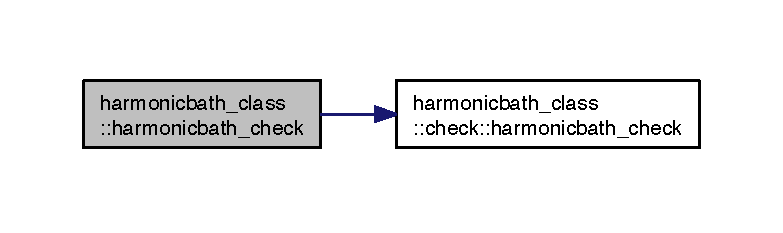
\includegraphics[width=350pt]{classharmonicbath__class_abde7a862edc5c843e0665c6a6705bd74_cgraph}
\end{center}
\end{figure}


\hypertarget{classharmonicbath__class_af4ce5a2a61231e5612ff243262e9f993}{\index{harmonicbath\-\_\-class@{harmonicbath\-\_\-class}!harmonicbath\-\_\-display@{harmonicbath\-\_\-display}}
\index{harmonicbath\-\_\-display@{harmonicbath\-\_\-display}!harmonicbath_class@{harmonicbath\-\_\-class}}
\subsubsection[{harmonicbath\-\_\-display}]{\setlength{\rightskip}{0pt plus 5cm}subroutine harmonicbath\-\_\-class\-::harmonicbath\-\_\-display (
\begin{DoxyParamCaption}
\item[{type({\bf harmonicbath}), intent(in)}]{this, }
\item[{character$\ast$($\ast$), intent(in), optional}]{msg}
\end{DoxyParamCaption}
)\hspace{0.3cm}{\ttfamily [private]}}}\label{classharmonicbath__class_af4ce5a2a61231e5612ff243262e9f993}
\hypertarget{classharmonicbath__class_a7d869bb99a49aa520fe606e808d5feb5}{\index{harmonicbath\-\_\-class@{harmonicbath\-\_\-class}!harmonicbath\-\_\-init@{harmonicbath\-\_\-init}}
\index{harmonicbath\-\_\-init@{harmonicbath\-\_\-init}!harmonicbath_class@{harmonicbath\-\_\-class}}
\subsubsection[{harmonicbath\-\_\-init}]{\setlength{\rightskip}{0pt plus 5cm}subroutine harmonicbath\-\_\-class\-::harmonicbath\-\_\-init (
\begin{DoxyParamCaption}
\item[{type({\bf harmonicbath}), intent(inout)}]{this, }
\item[{character$\ast$($\ast$), intent(in), optional}]{file}
\end{DoxyParamCaption}
)\hspace{0.3cm}{\ttfamily [private]}}}\label{classharmonicbath__class_a7d869bb99a49aa520fe606e808d5feb5}


Here is the call graph for this function\-:
\nopagebreak
\begin{figure}[H]
\begin{center}
\leavevmode
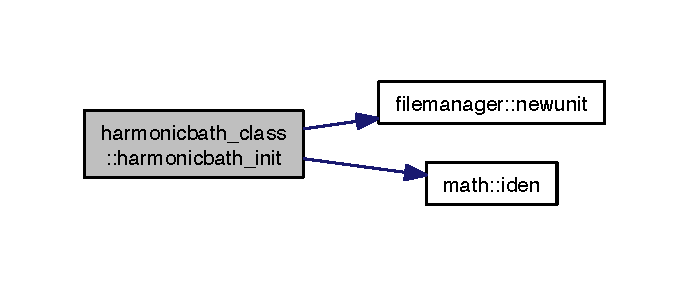
\includegraphics[width=330pt]{classharmonicbath__class_a7d869bb99a49aa520fe606e808d5feb5_cgraph}
\end{center}
\end{figure}


\hypertarget{classharmonicbath__class_ae4e0e1b027594bb77034f21e82f6ed63}{\index{harmonicbath\-\_\-class@{harmonicbath\-\_\-class}!harmonicbath\-\_\-kill@{harmonicbath\-\_\-kill}}
\index{harmonicbath\-\_\-kill@{harmonicbath\-\_\-kill}!harmonicbath_class@{harmonicbath\-\_\-class}}
\subsubsection[{harmonicbath\-\_\-kill}]{\setlength{\rightskip}{0pt plus 5cm}subroutine harmonicbath\-\_\-class\-::harmonicbath\-\_\-kill (
\begin{DoxyParamCaption}
\item[{type({\bf harmonicbath}), intent(inout)}]{this}
\end{DoxyParamCaption}
)\hspace{0.3cm}{\ttfamily [private]}}}\label{classharmonicbath__class_ae4e0e1b027594bb77034f21e82f6ed63}
\hypertarget{classharmonicbath__class_a6b27afcc7c1f24fec82adf3177d0adb8}{\index{harmonicbath\-\_\-class@{harmonicbath\-\_\-class}!harmonicbath\-\_\-resample@{harmonicbath\-\_\-resample}}
\index{harmonicbath\-\_\-resample@{harmonicbath\-\_\-resample}!harmonicbath_class@{harmonicbath\-\_\-class}}
\subsubsection[{harmonicbath\-\_\-resample}]{\setlength{\rightskip}{0pt plus 5cm}subroutine harmonicbath\-\_\-class\-::harmonicbath\-\_\-resample (
\begin{DoxyParamCaption}
\item[{type({\bf harmonicbath}), intent(inout)}]{this}
\end{DoxyParamCaption}
)\hspace{0.3cm}{\ttfamily [private]}}}\label{classharmonicbath__class_a6b27afcc7c1f24fec82adf3177d0adb8}


Here is the call graph for this function\-:
\nopagebreak
\begin{figure}[H]
\begin{center}
\leavevmode
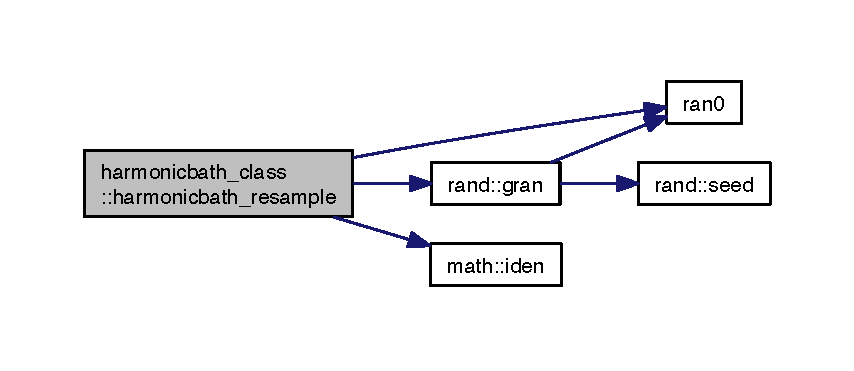
\includegraphics[width=350pt]{classharmonicbath__class_a6b27afcc7c1f24fec82adf3177d0adb8_cgraph}
\end{center}
\end{figure}


\hypertarget{classharmonicbath__class_a9dfb6e87e69957fcc4ec907135931ace}{\index{harmonicbath\-\_\-class@{harmonicbath\-\_\-class}!harmonicbath\-\_\-save@{harmonicbath\-\_\-save}}
\index{harmonicbath\-\_\-save@{harmonicbath\-\_\-save}!harmonicbath_class@{harmonicbath\-\_\-class}}
\subsubsection[{harmonicbath\-\_\-save}]{\setlength{\rightskip}{0pt plus 5cm}subroutine harmonicbath\-\_\-class\-::harmonicbath\-\_\-save (
\begin{DoxyParamCaption}
\item[{type({\bf harmonicbath}), intent(in)}]{this, }
\item[{character$\ast$($\ast$), intent(in)}]{file}
\end{DoxyParamCaption}
)\hspace{0.3cm}{\ttfamily [private]}}}\label{classharmonicbath__class_a9dfb6e87e69957fcc4ec907135931ace}


Here is the call graph for this function\-:
\nopagebreak
\begin{figure}[H]
\begin{center}
\leavevmode
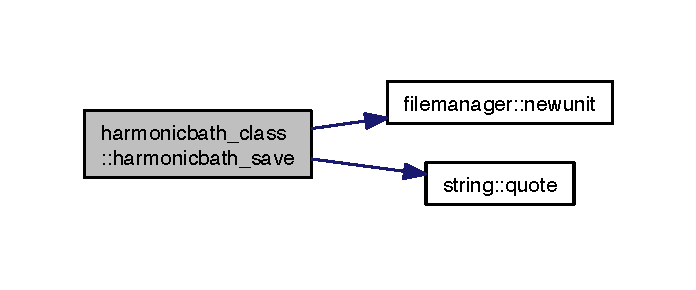
\includegraphics[width=334pt]{classharmonicbath__class_a9dfb6e87e69957fcc4ec907135931ace_cgraph}
\end{center}
\end{figure}


\hypertarget{classharmonicbath__class_ac930ca08461d767f4593374465c7229d}{\index{harmonicbath\-\_\-class@{harmonicbath\-\_\-class}!harmonicbath\-\_\-update@{harmonicbath\-\_\-update}}
\index{harmonicbath\-\_\-update@{harmonicbath\-\_\-update}!harmonicbath_class@{harmonicbath\-\_\-class}}
\subsubsection[{harmonicbath\-\_\-update}]{\setlength{\rightskip}{0pt plus 5cm}subroutine harmonicbath\-\_\-class\-::harmonicbath\-\_\-update (
\begin{DoxyParamCaption}
\item[{type({\bf harmonicbath}), intent(inout)}]{this}
\end{DoxyParamCaption}
)\hspace{0.3cm}{\ttfamily [private]}}}\label{classharmonicbath__class_ac930ca08461d767f4593374465c7229d}


The documentation for this module was generated from the following file\-:\begin{DoxyCompactItemize}
\item 
src/\hyperlink{harmonicbath_8f90}{harmonicbath.\-f90}\end{DoxyCompactItemize}

\hypertarget{structhb__class_1_1hb}{\section{hb\+\_\+class\+:\+:hb Type Reference}
\label{structhb__class_1_1hb}\index{hb\+\_\+class\+::hb@{hb\+\_\+class\+::hb}}
}
\subsection*{Private Attributes}
\begin{DoxyCompactItemize}
\item 
logical \hyperlink{structhb__class_1_1hb_ab15f7134343b95cad3a633262c4d1ae6}{initialized}
\item 
integer(long) \hyperlink{structhb__class_1_1hb_aa1ccd4393febf95c0c9b30f3e8b23bc3}{npart}
\item 
real(double), dimension(\+:), pointer \hyperlink{structhb__class_1_1hb_a245f6fbd55fe85b3c5c7dfda8e9aeadc}{mass}
\item 
real(double), dimension(\+:), pointer \hyperlink{structhb__class_1_1hb_adc2ac99589f86766e4d80c7a2d8eaa0c}{rmass}
\item 
real(double), dimension(\+:), pointer \hyperlink{structhb__class_1_1hb_ae5d949ad83b1c2491acca3fedb59127f}{charge}
\item 
integer(byte) \hyperlink{structhb__class_1_1hb_ab4c00922e761160b8ec3e3e3bcf41217}{ndim}
\item 
integer(long) \hyperlink{structhb__class_1_1hb_a0984c9d5bd990546d1b4b5f804ab3238}{ndof}
\item 
real(double), dimension(\+:), pointer \hyperlink{structhb__class_1_1hb_ad39d5d28f5be03c2bc6d00ecbc847e72}{qmin}
\item 
real(double), dimension(\+:), pointer \hyperlink{structhb__class_1_1hb_a097cb0c17e9a6557efa84d638650899b}{qmax}
\item 
logical, dimension(\+:), pointer \hyperlink{structhb__class_1_1hb_a076ab9d7a6a36a40529405c6fea62d70}{pbc}
\item 
real(double), dimension(\+:), pointer \hyperlink{structhb__class_1_1hb_aeb58002dd58afd2c2930db42209f19df}{q}
\item 
real(double), dimension(\+:), pointer \hyperlink{structhb__class_1_1hb_a138a258ac48be2d660556d987230a7b6}{p}
\item 
real(double), dimension(\+:), pointer \hyperlink{structhb__class_1_1hb_af871a155778593b68d1a0b12f20a9296}{f}
\item 
real(double) \hyperlink{structhb__class_1_1hb_ac20e5692850cd29066ed51b1f51b65ab}{v}
\item 
real(double) \hyperlink{structhb__class_1_1hb_aa9a64f5f6e1c6b43e49f4f369cc36122}{t}
\item 
real(double) \hyperlink{structhb__class_1_1hb_a5d5e5ee121dffd96571df21b84b83507}{temperature}
\item 
real(double), dimension(\+:), pointer \hyperlink{structhb__class_1_1hb_ac5b121a046f5ee32acc9830d4a9d0583}{mode}
\item 
real(double), dimension(\+:), pointer \hyperlink{structhb__class_1_1hb_aa5b032073db26bbc82430e5dcefa77a6}{w}
\item 
real(double), dimension(\+:,\+:), \\*
pointer \hyperlink{structhb__class_1_1hb_ac62b62b36a6c37ba8477efc35c6f97bf}{eigenvec}
\end{DoxyCompactItemize}


\subsection{Member Data Documentation}
\hypertarget{structhb__class_1_1hb_ae5d949ad83b1c2491acca3fedb59127f}{\index{hb\+\_\+class\+::hb@{hb\+\_\+class\+::hb}!charge@{charge}}
\index{charge@{charge}!hb\+\_\+class\+::hb@{hb\+\_\+class\+::hb}}
\subsubsection[{charge}]{\setlength{\rightskip}{0pt plus 5cm}real(double), dimension(\+:), pointer hb\+\_\+class\+::hb\+::charge\hspace{0.3cm}{\ttfamily [private]}}}\label{structhb__class_1_1hb_ae5d949ad83b1c2491acca3fedb59127f}
\hypertarget{structhb__class_1_1hb_ac62b62b36a6c37ba8477efc35c6f97bf}{\index{hb\+\_\+class\+::hb@{hb\+\_\+class\+::hb}!eigenvec@{eigenvec}}
\index{eigenvec@{eigenvec}!hb\+\_\+class\+::hb@{hb\+\_\+class\+::hb}}
\subsubsection[{eigenvec}]{\setlength{\rightskip}{0pt plus 5cm}real(double), dimension(\+:,\+:), pointer hb\+\_\+class\+::hb\+::eigenvec\hspace{0.3cm}{\ttfamily [private]}}}\label{structhb__class_1_1hb_ac62b62b36a6c37ba8477efc35c6f97bf}
\hypertarget{structhb__class_1_1hb_af871a155778593b68d1a0b12f20a9296}{\index{hb\+\_\+class\+::hb@{hb\+\_\+class\+::hb}!f@{f}}
\index{f@{f}!hb\+\_\+class\+::hb@{hb\+\_\+class\+::hb}}
\subsubsection[{f}]{\setlength{\rightskip}{0pt plus 5cm}real(double), dimension(\+:), pointer hb\+\_\+class\+::hb\+::f\hspace{0.3cm}{\ttfamily [private]}}}\label{structhb__class_1_1hb_af871a155778593b68d1a0b12f20a9296}
\hypertarget{structhb__class_1_1hb_ab15f7134343b95cad3a633262c4d1ae6}{\index{hb\+\_\+class\+::hb@{hb\+\_\+class\+::hb}!initialized@{initialized}}
\index{initialized@{initialized}!hb\+\_\+class\+::hb@{hb\+\_\+class\+::hb}}
\subsubsection[{initialized}]{\setlength{\rightskip}{0pt plus 5cm}logical hb\+\_\+class\+::hb\+::initialized\hspace{0.3cm}{\ttfamily [private]}}}\label{structhb__class_1_1hb_ab15f7134343b95cad3a633262c4d1ae6}
\hypertarget{structhb__class_1_1hb_a245f6fbd55fe85b3c5c7dfda8e9aeadc}{\index{hb\+\_\+class\+::hb@{hb\+\_\+class\+::hb}!mass@{mass}}
\index{mass@{mass}!hb\+\_\+class\+::hb@{hb\+\_\+class\+::hb}}
\subsubsection[{mass}]{\setlength{\rightskip}{0pt plus 5cm}real(double), dimension(\+:), pointer hb\+\_\+class\+::hb\+::mass\hspace{0.3cm}{\ttfamily [private]}}}\label{structhb__class_1_1hb_a245f6fbd55fe85b3c5c7dfda8e9aeadc}
\hypertarget{structhb__class_1_1hb_ac5b121a046f5ee32acc9830d4a9d0583}{\index{hb\+\_\+class\+::hb@{hb\+\_\+class\+::hb}!mode@{mode}}
\index{mode@{mode}!hb\+\_\+class\+::hb@{hb\+\_\+class\+::hb}}
\subsubsection[{mode}]{\setlength{\rightskip}{0pt plus 5cm}real(double), dimension(\+:), pointer hb\+\_\+class\+::hb\+::mode\hspace{0.3cm}{\ttfamily [private]}}}\label{structhb__class_1_1hb_ac5b121a046f5ee32acc9830d4a9d0583}
\hypertarget{structhb__class_1_1hb_ab4c00922e761160b8ec3e3e3bcf41217}{\index{hb\+\_\+class\+::hb@{hb\+\_\+class\+::hb}!ndim@{ndim}}
\index{ndim@{ndim}!hb\+\_\+class\+::hb@{hb\+\_\+class\+::hb}}
\subsubsection[{ndim}]{\setlength{\rightskip}{0pt plus 5cm}integer(byte) hb\+\_\+class\+::hb\+::ndim\hspace{0.3cm}{\ttfamily [private]}}}\label{structhb__class_1_1hb_ab4c00922e761160b8ec3e3e3bcf41217}
\hypertarget{structhb__class_1_1hb_a0984c9d5bd990546d1b4b5f804ab3238}{\index{hb\+\_\+class\+::hb@{hb\+\_\+class\+::hb}!ndof@{ndof}}
\index{ndof@{ndof}!hb\+\_\+class\+::hb@{hb\+\_\+class\+::hb}}
\subsubsection[{ndof}]{\setlength{\rightskip}{0pt plus 5cm}integer(long) hb\+\_\+class\+::hb\+::ndof\hspace{0.3cm}{\ttfamily [private]}}}\label{structhb__class_1_1hb_a0984c9d5bd990546d1b4b5f804ab3238}
\hypertarget{structhb__class_1_1hb_aa1ccd4393febf95c0c9b30f3e8b23bc3}{\index{hb\+\_\+class\+::hb@{hb\+\_\+class\+::hb}!npart@{npart}}
\index{npart@{npart}!hb\+\_\+class\+::hb@{hb\+\_\+class\+::hb}}
\subsubsection[{npart}]{\setlength{\rightskip}{0pt plus 5cm}integer(long) hb\+\_\+class\+::hb\+::npart\hspace{0.3cm}{\ttfamily [private]}}}\label{structhb__class_1_1hb_aa1ccd4393febf95c0c9b30f3e8b23bc3}
\hypertarget{structhb__class_1_1hb_a138a258ac48be2d660556d987230a7b6}{\index{hb\+\_\+class\+::hb@{hb\+\_\+class\+::hb}!p@{p}}
\index{p@{p}!hb\+\_\+class\+::hb@{hb\+\_\+class\+::hb}}
\subsubsection[{p}]{\setlength{\rightskip}{0pt plus 5cm}real(double), dimension(\+:), pointer hb\+\_\+class\+::hb\+::p\hspace{0.3cm}{\ttfamily [private]}}}\label{structhb__class_1_1hb_a138a258ac48be2d660556d987230a7b6}
\hypertarget{structhb__class_1_1hb_a076ab9d7a6a36a40529405c6fea62d70}{\index{hb\+\_\+class\+::hb@{hb\+\_\+class\+::hb}!pbc@{pbc}}
\index{pbc@{pbc}!hb\+\_\+class\+::hb@{hb\+\_\+class\+::hb}}
\subsubsection[{pbc}]{\setlength{\rightskip}{0pt plus 5cm}logical, dimension(\+:), pointer hb\+\_\+class\+::hb\+::pbc\hspace{0.3cm}{\ttfamily [private]}}}\label{structhb__class_1_1hb_a076ab9d7a6a36a40529405c6fea62d70}
\hypertarget{structhb__class_1_1hb_aeb58002dd58afd2c2930db42209f19df}{\index{hb\+\_\+class\+::hb@{hb\+\_\+class\+::hb}!q@{q}}
\index{q@{q}!hb\+\_\+class\+::hb@{hb\+\_\+class\+::hb}}
\subsubsection[{q}]{\setlength{\rightskip}{0pt plus 5cm}real(double), dimension(\+:), pointer hb\+\_\+class\+::hb\+::q\hspace{0.3cm}{\ttfamily [private]}}}\label{structhb__class_1_1hb_aeb58002dd58afd2c2930db42209f19df}
\hypertarget{structhb__class_1_1hb_a097cb0c17e9a6557efa84d638650899b}{\index{hb\+\_\+class\+::hb@{hb\+\_\+class\+::hb}!qmax@{qmax}}
\index{qmax@{qmax}!hb\+\_\+class\+::hb@{hb\+\_\+class\+::hb}}
\subsubsection[{qmax}]{\setlength{\rightskip}{0pt plus 5cm}real(double), dimension(\+:), pointer hb\+\_\+class\+::hb\+::qmax\hspace{0.3cm}{\ttfamily [private]}}}\label{structhb__class_1_1hb_a097cb0c17e9a6557efa84d638650899b}
\hypertarget{structhb__class_1_1hb_ad39d5d28f5be03c2bc6d00ecbc847e72}{\index{hb\+\_\+class\+::hb@{hb\+\_\+class\+::hb}!qmin@{qmin}}
\index{qmin@{qmin}!hb\+\_\+class\+::hb@{hb\+\_\+class\+::hb}}
\subsubsection[{qmin}]{\setlength{\rightskip}{0pt plus 5cm}real(double), dimension(\+:), pointer hb\+\_\+class\+::hb\+::qmin\hspace{0.3cm}{\ttfamily [private]}}}\label{structhb__class_1_1hb_ad39d5d28f5be03c2bc6d00ecbc847e72}
\hypertarget{structhb__class_1_1hb_adc2ac99589f86766e4d80c7a2d8eaa0c}{\index{hb\+\_\+class\+::hb@{hb\+\_\+class\+::hb}!rmass@{rmass}}
\index{rmass@{rmass}!hb\+\_\+class\+::hb@{hb\+\_\+class\+::hb}}
\subsubsection[{rmass}]{\setlength{\rightskip}{0pt plus 5cm}real(double), dimension(\+:), pointer hb\+\_\+class\+::hb\+::rmass\hspace{0.3cm}{\ttfamily [private]}}}\label{structhb__class_1_1hb_adc2ac99589f86766e4d80c7a2d8eaa0c}
\hypertarget{structhb__class_1_1hb_aa9a64f5f6e1c6b43e49f4f369cc36122}{\index{hb\+\_\+class\+::hb@{hb\+\_\+class\+::hb}!t@{t}}
\index{t@{t}!hb\+\_\+class\+::hb@{hb\+\_\+class\+::hb}}
\subsubsection[{t}]{\setlength{\rightskip}{0pt plus 5cm}real(double) hb\+\_\+class\+::hb\+::t\hspace{0.3cm}{\ttfamily [private]}}}\label{structhb__class_1_1hb_aa9a64f5f6e1c6b43e49f4f369cc36122}
\hypertarget{structhb__class_1_1hb_a5d5e5ee121dffd96571df21b84b83507}{\index{hb\+\_\+class\+::hb@{hb\+\_\+class\+::hb}!temperature@{temperature}}
\index{temperature@{temperature}!hb\+\_\+class\+::hb@{hb\+\_\+class\+::hb}}
\subsubsection[{temperature}]{\setlength{\rightskip}{0pt plus 5cm}real(double) hb\+\_\+class\+::hb\+::temperature\hspace{0.3cm}{\ttfamily [private]}}}\label{structhb__class_1_1hb_a5d5e5ee121dffd96571df21b84b83507}
\hypertarget{structhb__class_1_1hb_ac20e5692850cd29066ed51b1f51b65ab}{\index{hb\+\_\+class\+::hb@{hb\+\_\+class\+::hb}!v@{v}}
\index{v@{v}!hb\+\_\+class\+::hb@{hb\+\_\+class\+::hb}}
\subsubsection[{v}]{\setlength{\rightskip}{0pt plus 5cm}real(double) hb\+\_\+class\+::hb\+::v\hspace{0.3cm}{\ttfamily [private]}}}\label{structhb__class_1_1hb_ac20e5692850cd29066ed51b1f51b65ab}
\hypertarget{structhb__class_1_1hb_aa5b032073db26bbc82430e5dcefa77a6}{\index{hb\+\_\+class\+::hb@{hb\+\_\+class\+::hb}!w@{w}}
\index{w@{w}!hb\+\_\+class\+::hb@{hb\+\_\+class\+::hb}}
\subsubsection[{w}]{\setlength{\rightskip}{0pt plus 5cm}real(double), dimension(\+:), pointer hb\+\_\+class\+::hb\+::w\hspace{0.3cm}{\ttfamily [private]}}}\label{structhb__class_1_1hb_aa5b032073db26bbc82430e5dcefa77a6}


The documentation for this type was generated from the following files\+:\begin{DoxyCompactItemize}
\item 
src/\hyperlink{hb_8f90}{hb.\+f90}\item 
src/\hyperlink{hbcopy_8f90}{hbcopy.\+f90}\end{DoxyCompactItemize}

\hypertarget{classhb__class}{\section{hb\+\_\+class Module Reference}
\label{classhb__class}\index{hb\+\_\+class@{hb\+\_\+class}}
}


Classical Subsystem Primitive.  


\subsection*{Data Types}
\begin{DoxyCompactItemize}
\item 
interface \hyperlink{interfacehb__class_1_1check}{check}
\item 
interface \hyperlink{interfacehb__class_1_1display}{display}
\item 
type \hyperlink{structhb__class_1_1hb}{hb}
\item 
interface \hyperlink{interfacehb__class_1_1kill}{kill}
\item 
interface \hyperlink{interfacehb__class_1_1new}{new}
\item 
interface \hyperlink{interfacehb__class_1_1resample}{resample}
\item 
interface \hyperlink{interfacehb__class_1_1save}{save}
\item 
interface \hyperlink{interfacehb__class_1_1update}{update}
\end{DoxyCompactItemize}
\subsection*{Private Member Functions}
\begin{DoxyCompactItemize}
\item 
subroutine \hyperlink{classhb__class_aad89f206670f2c2396f92abf66cf9c1d}{hb\+\_\+init} (this, file)
\item 
subroutine \hyperlink{classhb__class_a696c9e145feab6ab780338ffcf6d6d4b}{hb\+\_\+kill} (this)
\item 
subroutine \hyperlink{classhb__class_a03d6e94665987e6ce2a283953632fb3f}{hb\+\_\+update} (this)
\item 
subroutine \hyperlink{classhb__class_a9d6faaa888c003d629e1b35f8b510832}{hb\+\_\+resample} (this)
\item 
subroutine \hyperlink{classhb__class_a8d8a7109913e9189fbc950d34378727b}{hb\+\_\+display} (this, msg)
\item 
subroutine \hyperlink{classhb__class_a53b39344e155580d8d2161a497774364}{hb\+\_\+save} (this, file)
\item 
integer(short) function \hyperlink{classhb__class_a84c1c4284b5897ff912c8c1671b6775f}{hb\+\_\+check} (this)
\item 
subroutine \hyperlink{classhb__class_aad89f206670f2c2396f92abf66cf9c1d}{hb\+\_\+init} (this, file)
\item 
subroutine \hyperlink{classhb__class_a696c9e145feab6ab780338ffcf6d6d4b}{hb\+\_\+kill} (this)
\item 
subroutine \hyperlink{classhb__class_a03d6e94665987e6ce2a283953632fb3f}{hb\+\_\+update} (this)
\item 
subroutine \hyperlink{classhb__class_a9d6faaa888c003d629e1b35f8b510832}{hb\+\_\+resample} (this)
\item 
subroutine \hyperlink{classhb__class_a8d8a7109913e9189fbc950d34378727b}{hb\+\_\+display} (this, msg)
\item 
subroutine \hyperlink{classhb__class_a53b39344e155580d8d2161a497774364}{hb\+\_\+save} (this, file)
\item 
integer(short) function \hyperlink{classhb__class_a84c1c4284b5897ff912c8c1671b6775f}{hb\+\_\+check} (this)
\end{DoxyCompactItemize}


\subsection{Detailed Description}
Classical Subsystem Primitive. 

This class defines the classical subsystem kernal inherited by all derived classical subsystems. \begin{DoxyDate}{Date}
12 Nov 2012 
\end{DoxyDate}
\begin{DoxyAuthor}{Authors}
Daniel Montemayor 
\end{DoxyAuthor}


\subsection{Member Function/\+Subroutine Documentation}
\hypertarget{classhb__class_a84c1c4284b5897ff912c8c1671b6775f}{\index{hb\+\_\+class@{hb\+\_\+class}!hb\+\_\+check@{hb\+\_\+check}}
\index{hb\+\_\+check@{hb\+\_\+check}!hb\+\_\+class@{hb\+\_\+class}}
\subsubsection[{hb\+\_\+check}]{\setlength{\rightskip}{0pt plus 5cm}integer(short) function hb\+\_\+class\+::hb\+\_\+check (
\begin{DoxyParamCaption}
\item[{type({\bf hb}), intent(in)}]{this}
\end{DoxyParamCaption}
)\hspace{0.3cm}{\ttfamily [private]}}}\label{classhb__class_a84c1c4284b5897ff912c8c1671b6775f}


Here is the call graph for this function\+:\nopagebreak
\begin{figure}[H]
\begin{center}
\leavevmode
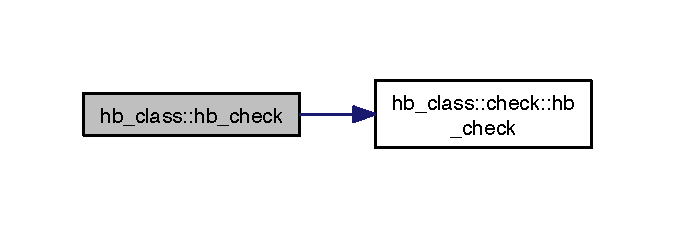
\includegraphics[width=324pt]{classhb__class_a84c1c4284b5897ff912c8c1671b6775f_cgraph}
\end{center}
\end{figure}


\hypertarget{classhb__class_a84c1c4284b5897ff912c8c1671b6775f}{\index{hb\+\_\+class@{hb\+\_\+class}!hb\+\_\+check@{hb\+\_\+check}}
\index{hb\+\_\+check@{hb\+\_\+check}!hb\+\_\+class@{hb\+\_\+class}}
\subsubsection[{hb\+\_\+check}]{\setlength{\rightskip}{0pt plus 5cm}integer(short) function hb\+\_\+class\+::hb\+\_\+check (
\begin{DoxyParamCaption}
\item[{type({\bf hb}), intent(in)}]{this}
\end{DoxyParamCaption}
)\hspace{0.3cm}{\ttfamily [private]}}}\label{classhb__class_a84c1c4284b5897ff912c8c1671b6775f}


Here is the call graph for this function\+:\nopagebreak
\begin{figure}[H]
\begin{center}
\leavevmode
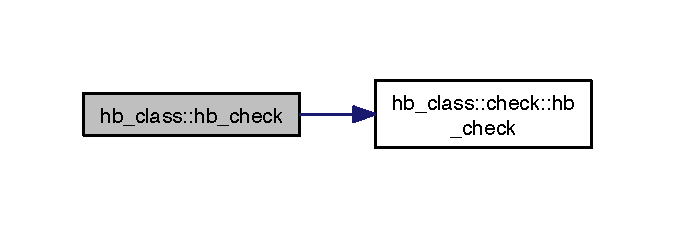
\includegraphics[width=324pt]{classhb__class_a84c1c4284b5897ff912c8c1671b6775f_cgraph}
\end{center}
\end{figure}


\hypertarget{classhb__class_a8d8a7109913e9189fbc950d34378727b}{\index{hb\+\_\+class@{hb\+\_\+class}!hb\+\_\+display@{hb\+\_\+display}}
\index{hb\+\_\+display@{hb\+\_\+display}!hb\+\_\+class@{hb\+\_\+class}}
\subsubsection[{hb\+\_\+display}]{\setlength{\rightskip}{0pt plus 5cm}subroutine hb\+\_\+class\+::hb\+\_\+display (
\begin{DoxyParamCaption}
\item[{type({\bf hb}), intent(in)}]{this, }
\item[{character$\ast$($\ast$), intent(in), optional}]{msg}
\end{DoxyParamCaption}
)\hspace{0.3cm}{\ttfamily [private]}}}\label{classhb__class_a8d8a7109913e9189fbc950d34378727b}
\hypertarget{classhb__class_a8d8a7109913e9189fbc950d34378727b}{\index{hb\+\_\+class@{hb\+\_\+class}!hb\+\_\+display@{hb\+\_\+display}}
\index{hb\+\_\+display@{hb\+\_\+display}!hb\+\_\+class@{hb\+\_\+class}}
\subsubsection[{hb\+\_\+display}]{\setlength{\rightskip}{0pt plus 5cm}subroutine hb\+\_\+class\+::hb\+\_\+display (
\begin{DoxyParamCaption}
\item[{type({\bf hb}), intent(in)}]{this, }
\item[{character$\ast$($\ast$), intent(in), optional}]{msg}
\end{DoxyParamCaption}
)\hspace{0.3cm}{\ttfamily [private]}}}\label{classhb__class_a8d8a7109913e9189fbc950d34378727b}
\hypertarget{classhb__class_aad89f206670f2c2396f92abf66cf9c1d}{\index{hb\+\_\+class@{hb\+\_\+class}!hb\+\_\+init@{hb\+\_\+init}}
\index{hb\+\_\+init@{hb\+\_\+init}!hb\+\_\+class@{hb\+\_\+class}}
\subsubsection[{hb\+\_\+init}]{\setlength{\rightskip}{0pt plus 5cm}subroutine hb\+\_\+class\+::hb\+\_\+init (
\begin{DoxyParamCaption}
\item[{type({\bf hb}), intent(inout)}]{this, }
\item[{character$\ast$($\ast$), intent(in), optional}]{file}
\end{DoxyParamCaption}
)\hspace{0.3cm}{\ttfamily [private]}}}\label{classhb__class_aad89f206670f2c2396f92abf66cf9c1d}


Here is the call graph for this function\+:\nopagebreak
\begin{figure}[H]
\begin{center}
\leavevmode
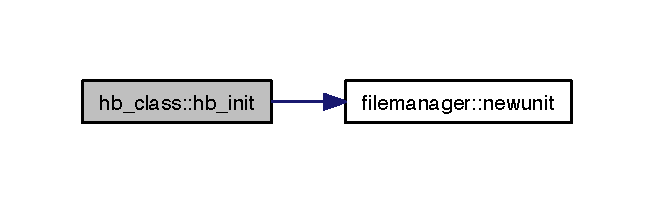
\includegraphics[width=313pt]{classhb__class_aad89f206670f2c2396f92abf66cf9c1d_cgraph}
\end{center}
\end{figure}


\hypertarget{classhb__class_aad89f206670f2c2396f92abf66cf9c1d}{\index{hb\+\_\+class@{hb\+\_\+class}!hb\+\_\+init@{hb\+\_\+init}}
\index{hb\+\_\+init@{hb\+\_\+init}!hb\+\_\+class@{hb\+\_\+class}}
\subsubsection[{hb\+\_\+init}]{\setlength{\rightskip}{0pt plus 5cm}subroutine hb\+\_\+class\+::hb\+\_\+init (
\begin{DoxyParamCaption}
\item[{type({\bf hb}), intent(inout)}]{this, }
\item[{character$\ast$($\ast$), intent(in), optional}]{file}
\end{DoxyParamCaption}
)\hspace{0.3cm}{\ttfamily [private]}}}\label{classhb__class_aad89f206670f2c2396f92abf66cf9c1d}


Here is the call graph for this function\+:\nopagebreak
\begin{figure}[H]
\begin{center}
\leavevmode
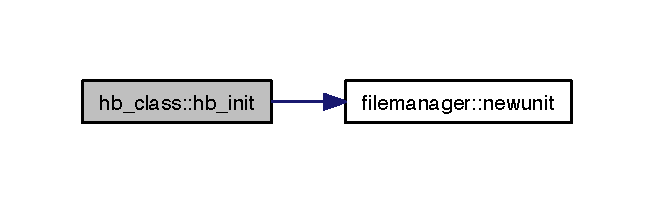
\includegraphics[width=313pt]{classhb__class_aad89f206670f2c2396f92abf66cf9c1d_cgraph}
\end{center}
\end{figure}


\hypertarget{classhb__class_a696c9e145feab6ab780338ffcf6d6d4b}{\index{hb\+\_\+class@{hb\+\_\+class}!hb\+\_\+kill@{hb\+\_\+kill}}
\index{hb\+\_\+kill@{hb\+\_\+kill}!hb\+\_\+class@{hb\+\_\+class}}
\subsubsection[{hb\+\_\+kill}]{\setlength{\rightskip}{0pt plus 5cm}subroutine hb\+\_\+class\+::hb\+\_\+kill (
\begin{DoxyParamCaption}
\item[{type({\bf hb}), intent(inout)}]{this}
\end{DoxyParamCaption}
)\hspace{0.3cm}{\ttfamily [private]}}}\label{classhb__class_a696c9e145feab6ab780338ffcf6d6d4b}
\hypertarget{classhb__class_a696c9e145feab6ab780338ffcf6d6d4b}{\index{hb\+\_\+class@{hb\+\_\+class}!hb\+\_\+kill@{hb\+\_\+kill}}
\index{hb\+\_\+kill@{hb\+\_\+kill}!hb\+\_\+class@{hb\+\_\+class}}
\subsubsection[{hb\+\_\+kill}]{\setlength{\rightskip}{0pt plus 5cm}subroutine hb\+\_\+class\+::hb\+\_\+kill (
\begin{DoxyParamCaption}
\item[{type({\bf hb}), intent(inout)}]{this}
\end{DoxyParamCaption}
)\hspace{0.3cm}{\ttfamily [private]}}}\label{classhb__class_a696c9e145feab6ab780338ffcf6d6d4b}
\hypertarget{classhb__class_a9d6faaa888c003d629e1b35f8b510832}{\index{hb\+\_\+class@{hb\+\_\+class}!hb\+\_\+resample@{hb\+\_\+resample}}
\index{hb\+\_\+resample@{hb\+\_\+resample}!hb\+\_\+class@{hb\+\_\+class}}
\subsubsection[{hb\+\_\+resample}]{\setlength{\rightskip}{0pt plus 5cm}subroutine hb\+\_\+class\+::hb\+\_\+resample (
\begin{DoxyParamCaption}
\item[{type({\bf hb}), intent(inout)}]{this}
\end{DoxyParamCaption}
)\hspace{0.3cm}{\ttfamily [private]}}}\label{classhb__class_a9d6faaa888c003d629e1b35f8b510832}
\hypertarget{classhb__class_a9d6faaa888c003d629e1b35f8b510832}{\index{hb\+\_\+class@{hb\+\_\+class}!hb\+\_\+resample@{hb\+\_\+resample}}
\index{hb\+\_\+resample@{hb\+\_\+resample}!hb\+\_\+class@{hb\+\_\+class}}
\subsubsection[{hb\+\_\+resample}]{\setlength{\rightskip}{0pt plus 5cm}subroutine hb\+\_\+class\+::hb\+\_\+resample (
\begin{DoxyParamCaption}
\item[{type({\bf hb}), intent(inout)}]{this}
\end{DoxyParamCaption}
)\hspace{0.3cm}{\ttfamily [private]}}}\label{classhb__class_a9d6faaa888c003d629e1b35f8b510832}
\hypertarget{classhb__class_a53b39344e155580d8d2161a497774364}{\index{hb\+\_\+class@{hb\+\_\+class}!hb\+\_\+save@{hb\+\_\+save}}
\index{hb\+\_\+save@{hb\+\_\+save}!hb\+\_\+class@{hb\+\_\+class}}
\subsubsection[{hb\+\_\+save}]{\setlength{\rightskip}{0pt plus 5cm}subroutine hb\+\_\+class\+::hb\+\_\+save (
\begin{DoxyParamCaption}
\item[{type({\bf hb}), intent(in)}]{this, }
\item[{character$\ast$($\ast$), intent(in)}]{file}
\end{DoxyParamCaption}
)\hspace{0.3cm}{\ttfamily [private]}}}\label{classhb__class_a53b39344e155580d8d2161a497774364}


Here is the call graph for this function\+:\nopagebreak
\begin{figure}[H]
\begin{center}
\leavevmode
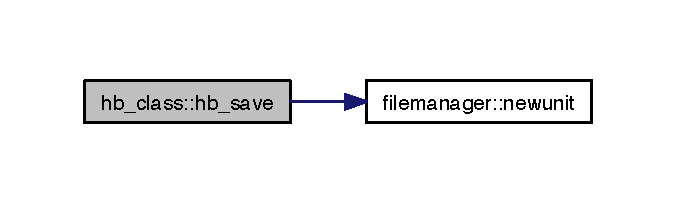
\includegraphics[width=321pt]{classhb__class_a53b39344e155580d8d2161a497774364_cgraph}
\end{center}
\end{figure}


\hypertarget{classhb__class_a53b39344e155580d8d2161a497774364}{\index{hb\+\_\+class@{hb\+\_\+class}!hb\+\_\+save@{hb\+\_\+save}}
\index{hb\+\_\+save@{hb\+\_\+save}!hb\+\_\+class@{hb\+\_\+class}}
\subsubsection[{hb\+\_\+save}]{\setlength{\rightskip}{0pt plus 5cm}subroutine hb\+\_\+class\+::hb\+\_\+save (
\begin{DoxyParamCaption}
\item[{type({\bf hb}), intent(in)}]{this, }
\item[{character$\ast$($\ast$), intent(in)}]{file}
\end{DoxyParamCaption}
)\hspace{0.3cm}{\ttfamily [private]}}}\label{classhb__class_a53b39344e155580d8d2161a497774364}


Here is the call graph for this function\+:\nopagebreak
\begin{figure}[H]
\begin{center}
\leavevmode
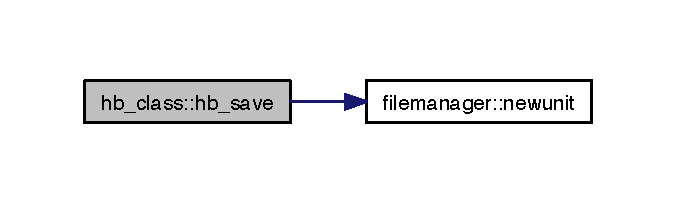
\includegraphics[width=321pt]{classhb__class_a53b39344e155580d8d2161a497774364_cgraph}
\end{center}
\end{figure}


\hypertarget{classhb__class_a03d6e94665987e6ce2a283953632fb3f}{\index{hb\+\_\+class@{hb\+\_\+class}!hb\+\_\+update@{hb\+\_\+update}}
\index{hb\+\_\+update@{hb\+\_\+update}!hb\+\_\+class@{hb\+\_\+class}}
\subsubsection[{hb\+\_\+update}]{\setlength{\rightskip}{0pt plus 5cm}subroutine hb\+\_\+class\+::hb\+\_\+update (
\begin{DoxyParamCaption}
\item[{type({\bf hb}), intent(inout)}]{this}
\end{DoxyParamCaption}
)\hspace{0.3cm}{\ttfamily [private]}}}\label{classhb__class_a03d6e94665987e6ce2a283953632fb3f}
\hypertarget{classhb__class_a03d6e94665987e6ce2a283953632fb3f}{\index{hb\+\_\+class@{hb\+\_\+class}!hb\+\_\+update@{hb\+\_\+update}}
\index{hb\+\_\+update@{hb\+\_\+update}!hb\+\_\+class@{hb\+\_\+class}}
\subsubsection[{hb\+\_\+update}]{\setlength{\rightskip}{0pt plus 5cm}subroutine hb\+\_\+class\+::hb\+\_\+update (
\begin{DoxyParamCaption}
\item[{type({\bf hb}), intent(inout)}]{this}
\end{DoxyParamCaption}
)\hspace{0.3cm}{\ttfamily [private]}}}\label{classhb__class_a03d6e94665987e6ce2a283953632fb3f}


The documentation for this module was generated from the following files\+:\begin{DoxyCompactItemize}
\item 
src/\hyperlink{hb_8f90}{hb.\+f90}\item 
src/\hyperlink{hbcopy_8f90}{hbcopy.\+f90}\end{DoxyCompactItemize}

\hypertarget{structhc__class_1_1hc}{}\section{hc\+\_\+class\+:\+:hc Type Reference}
\label{structhc__class_1_1hc}\index{hc\+\_\+class\+::hc@{hc\+\_\+class\+::hc}}


Collaboration diagram for hc\+\_\+class\+:\+:hc\+:\nopagebreak
\begin{figure}[H]
\begin{center}
\leavevmode
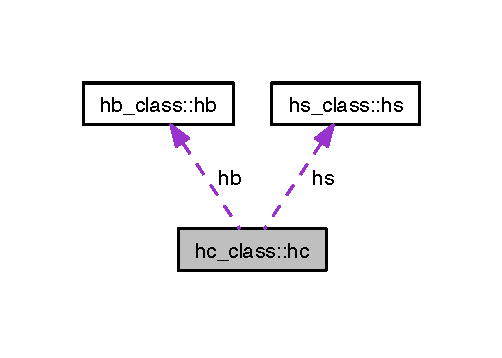
\includegraphics[width=241pt]{structhc__class_1_1hc__coll__graph}
\end{center}
\end{figure}
\subsection*{Private Attributes}
\begin{DoxyCompactItemize}
\item 
logical \hyperlink{structhc__class_1_1hc_a89151c80172cb67d68a44b6264afb8a7}{initialized}
\item 
type(\hyperlink{strucths__class_1_1hs}{hs}), pointer \hyperlink{structhc__class_1_1hc_a09dd08ce79ada0e7a9f7c3eb8a2a50f5}{hs}
\item 
type(\hyperlink{structhb__class_1_1hb}{hb}), pointer \hyperlink{structhc__class_1_1hc_a87af1d9489543e7f6a7501ea8468f763}{hb}
\item 
complex(double), dimension(\+:,\+:), pointer \hyperlink{structhc__class_1_1hc_ad3bab6b18bd729b4e1c49f7d14c0b4f9}{v}
\item 
complex(double), dimension(\+:,\+:,\+:), pointer \hyperlink{structhc__class_1_1hc_ae44fb8b1351b045650148c174099a1a1}{dv}
\end{DoxyCompactItemize}


\subsection{Member Data Documentation}
\mbox{\Hypertarget{structhc__class_1_1hc_ae44fb8b1351b045650148c174099a1a1}\label{structhc__class_1_1hc_ae44fb8b1351b045650148c174099a1a1}} 
\index{hc\+\_\+class\+::hc@{hc\+\_\+class\+::hc}!dv@{dv}}
\index{dv@{dv}!hc\+\_\+class\+::hc@{hc\+\_\+class\+::hc}}
\subsubsection{\texorpdfstring{dv}{dv}}
{\footnotesize\ttfamily complex(double), dimension(\+:,\+:,\+:), pointer hc\+\_\+class\+::hc\+::dv\hspace{0.3cm}{\ttfamily [private]}}

\mbox{\Hypertarget{structhc__class_1_1hc_a87af1d9489543e7f6a7501ea8468f763}\label{structhc__class_1_1hc_a87af1d9489543e7f6a7501ea8468f763}} 
\index{hc\+\_\+class\+::hc@{hc\+\_\+class\+::hc}!hb@{hb}}
\index{hb@{hb}!hc\+\_\+class\+::hc@{hc\+\_\+class\+::hc}}
\subsubsection{\texorpdfstring{hb}{hb}}
{\footnotesize\ttfamily type(\hyperlink{structhb__class_1_1hb}{hb}), pointer hc\+\_\+class\+::hc\+::hb\hspace{0.3cm}{\ttfamily [private]}}

\mbox{\Hypertarget{structhc__class_1_1hc_a09dd08ce79ada0e7a9f7c3eb8a2a50f5}\label{structhc__class_1_1hc_a09dd08ce79ada0e7a9f7c3eb8a2a50f5}} 
\index{hc\+\_\+class\+::hc@{hc\+\_\+class\+::hc}!hs@{hs}}
\index{hs@{hs}!hc\+\_\+class\+::hc@{hc\+\_\+class\+::hc}}
\subsubsection{\texorpdfstring{hs}{hs}}
{\footnotesize\ttfamily type(\hyperlink{strucths__class_1_1hs}{hs}), pointer hc\+\_\+class\+::hc\+::hs\hspace{0.3cm}{\ttfamily [private]}}

\mbox{\Hypertarget{structhc__class_1_1hc_a89151c80172cb67d68a44b6264afb8a7}\label{structhc__class_1_1hc_a89151c80172cb67d68a44b6264afb8a7}} 
\index{hc\+\_\+class\+::hc@{hc\+\_\+class\+::hc}!initialized@{initialized}}
\index{initialized@{initialized}!hc\+\_\+class\+::hc@{hc\+\_\+class\+::hc}}
\subsubsection{\texorpdfstring{initialized}{initialized}}
{\footnotesize\ttfamily logical hc\+\_\+class\+::hc\+::initialized\hspace{0.3cm}{\ttfamily [private]}}

\mbox{\Hypertarget{structhc__class_1_1hc_ad3bab6b18bd729b4e1c49f7d14c0b4f9}\label{structhc__class_1_1hc_ad3bab6b18bd729b4e1c49f7d14c0b4f9}} 
\index{hc\+\_\+class\+::hc@{hc\+\_\+class\+::hc}!v@{v}}
\index{v@{v}!hc\+\_\+class\+::hc@{hc\+\_\+class\+::hc}}
\subsubsection{\texorpdfstring{v}{v}}
{\footnotesize\ttfamily complex(double), dimension(\+:,\+:), pointer hc\+\_\+class\+::hc\+::v\hspace{0.3cm}{\ttfamily [private]}}



The documentation for this type was generated from the following file\+:\begin{DoxyCompactItemize}
\item 
src/\hyperlink{hc_8f90}{hc.\+f90}\end{DoxyCompactItemize}

\hypertarget{classhc__class}{\section{hc\-\_\-class Module Reference}
\label{classhc__class}\index{hc\-\_\-class@{hc\-\_\-class}}
}


Coupling Term Primitive.  


\subsection*{Data Types}
\begin{DoxyCompactItemize}
\item 
interface \hyperlink{interfacehc__class_1_1check}{check}
\item 
interface \hyperlink{interfacehc__class_1_1display}{display}
\item 
type \hyperlink{structhc__class_1_1hc}{hc}
\item 
interface \hyperlink{interfacehc__class_1_1kill}{kill}
\item 
interface \hyperlink{interfacehc__class_1_1new}{new}
\item 
interface \hyperlink{interfacehc__class_1_1resample}{resample}
\item 
interface \hyperlink{interfacehc__class_1_1save}{save}
\item 
interface \hyperlink{interfacehc__class_1_1update}{update}
\end{DoxyCompactItemize}
\subsection*{Public Member Functions}
\begin{DoxyCompactItemize}
\item 
subroutine \hyperlink{classhc__class_a72759d56fe1bbe360bfe0efaae62b6a6}{hc\-\_\-kill} (this)
\end{DoxyCompactItemize}
\subsection*{Private Member Functions}
\begin{DoxyCompactItemize}
\item 
subroutine \hyperlink{classhc__class_a6a95655090afaac2c5f7b049c3919597}{hc\-\_\-init} (this, qs, cs, file)
\item 
subroutine \hyperlink{classhc__class_a5b4008b35ac8a501909a4b9aed8fcd71}{hc\-\_\-update} (this)
\item 
subroutine \hyperlink{classhc__class_a1b4a0d9a46c63f538c74670dca5fdc82}{hc\-\_\-resample} (this)
\item 
subroutine \hyperlink{classhc__class_a484af233bb8b65db73534ae297fa7346}{hc\-\_\-display} (this, msg)
\item 
subroutine \hyperlink{classhc__class_ac1fbe6abcc3415c55bd2b920cbb47234}{hc\-\_\-save} (this, file)
\item 
integer(short) function \hyperlink{classhc__class_ad0b55c92720ef59cfd8b4cecd194afe1}{hc\-\_\-check} (this)
\end{DoxyCompactItemize}


\subsection{Detailed Description}
Coupling Term Primitive. 

This class defines the coupling term kernal inherited by all derived coupling terms. \begin{DoxyAuthor}{Authors}
Daniel Montemayor 
\end{DoxyAuthor}


\subsection{Member Function/\-Subroutine Documentation}
\hypertarget{classhc__class_ad0b55c92720ef59cfd8b4cecd194afe1}{\index{hc\-\_\-class@{hc\-\_\-class}!hc\-\_\-check@{hc\-\_\-check}}
\index{hc\-\_\-check@{hc\-\_\-check}!hc_class@{hc\-\_\-class}}
\subsubsection[{hc\-\_\-check}]{\setlength{\rightskip}{0pt plus 5cm}integer(short) function hc\-\_\-class\-::hc\-\_\-check (
\begin{DoxyParamCaption}
\item[{type({\bf hc}), intent(in)}]{this}
\end{DoxyParamCaption}
)\hspace{0.3cm}{\ttfamily [private]}}}\label{classhc__class_ad0b55c92720ef59cfd8b4cecd194afe1}


Here is the call graph for this function\-:
\nopagebreak
\begin{figure}[H]
\begin{center}
\leavevmode
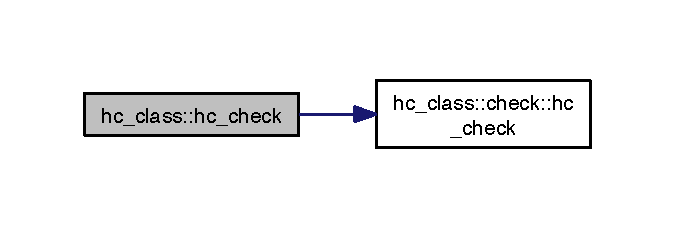
\includegraphics[width=324pt]{classhc__class_ad0b55c92720ef59cfd8b4cecd194afe1_cgraph}
\end{center}
\end{figure}


\hypertarget{classhc__class_a484af233bb8b65db73534ae297fa7346}{\index{hc\-\_\-class@{hc\-\_\-class}!hc\-\_\-display@{hc\-\_\-display}}
\index{hc\-\_\-display@{hc\-\_\-display}!hc_class@{hc\-\_\-class}}
\subsubsection[{hc\-\_\-display}]{\setlength{\rightskip}{0pt plus 5cm}subroutine hc\-\_\-class\-::hc\-\_\-display (
\begin{DoxyParamCaption}
\item[{type({\bf hc}), intent(in)}]{this, }
\item[{character$\ast$($\ast$), intent(in), optional}]{msg}
\end{DoxyParamCaption}
)\hspace{0.3cm}{\ttfamily [private]}}}\label{classhc__class_a484af233bb8b65db73534ae297fa7346}
\hypertarget{classhc__class_a6a95655090afaac2c5f7b049c3919597}{\index{hc\-\_\-class@{hc\-\_\-class}!hc\-\_\-init@{hc\-\_\-init}}
\index{hc\-\_\-init@{hc\-\_\-init}!hc_class@{hc\-\_\-class}}
\subsubsection[{hc\-\_\-init}]{\setlength{\rightskip}{0pt plus 5cm}subroutine hc\-\_\-class\-::hc\-\_\-init (
\begin{DoxyParamCaption}
\item[{type({\bf hc}), intent(inout)}]{this, }
\item[{type(quantum), intent(inout), target}]{qs, }
\item[{type(classical), intent(inout), target}]{cs, }
\item[{character$\ast$($\ast$), intent(in), optional}]{file}
\end{DoxyParamCaption}
)\hspace{0.3cm}{\ttfamily [private]}}}\label{classhc__class_a6a95655090afaac2c5f7b049c3919597}
\hypertarget{classhc__class_a72759d56fe1bbe360bfe0efaae62b6a6}{\index{hc\-\_\-class@{hc\-\_\-class}!hc\-\_\-kill@{hc\-\_\-kill}}
\index{hc\-\_\-kill@{hc\-\_\-kill}!hc_class@{hc\-\_\-class}}
\subsubsection[{hc\-\_\-kill}]{\setlength{\rightskip}{0pt plus 5cm}subroutine hc\-\_\-class\-::hc\-\_\-kill (
\begin{DoxyParamCaption}
\item[{type({\bf hc}), intent(inout)}]{this}
\end{DoxyParamCaption}
)}}\label{classhc__class_a72759d56fe1bbe360bfe0efaae62b6a6}
\hypertarget{classhc__class_a1b4a0d9a46c63f538c74670dca5fdc82}{\index{hc\-\_\-class@{hc\-\_\-class}!hc\-\_\-resample@{hc\-\_\-resample}}
\index{hc\-\_\-resample@{hc\-\_\-resample}!hc_class@{hc\-\_\-class}}
\subsubsection[{hc\-\_\-resample}]{\setlength{\rightskip}{0pt plus 5cm}subroutine hc\-\_\-class\-::hc\-\_\-resample (
\begin{DoxyParamCaption}
\item[{type({\bf hc}), intent(inout)}]{this}
\end{DoxyParamCaption}
)\hspace{0.3cm}{\ttfamily [private]}}}\label{classhc__class_a1b4a0d9a46c63f538c74670dca5fdc82}
\hypertarget{classhc__class_ac1fbe6abcc3415c55bd2b920cbb47234}{\index{hc\-\_\-class@{hc\-\_\-class}!hc\-\_\-save@{hc\-\_\-save}}
\index{hc\-\_\-save@{hc\-\_\-save}!hc_class@{hc\-\_\-class}}
\subsubsection[{hc\-\_\-save}]{\setlength{\rightskip}{0pt plus 5cm}subroutine hc\-\_\-class\-::hc\-\_\-save (
\begin{DoxyParamCaption}
\item[{type({\bf hc}), intent(in)}]{this, }
\item[{character$\ast$($\ast$)}]{file}
\end{DoxyParamCaption}
)\hspace{0.3cm}{\ttfamily [private]}}}\label{classhc__class_ac1fbe6abcc3415c55bd2b920cbb47234}


Here is the call graph for this function\-:
\nopagebreak
\begin{figure}[H]
\begin{center}
\leavevmode
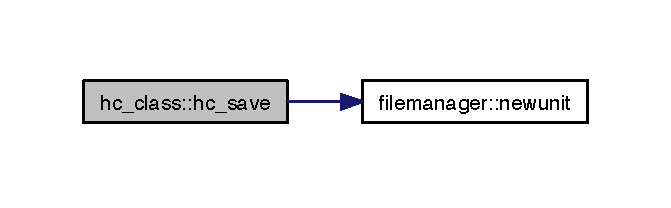
\includegraphics[width=322pt]{classhc__class_ac1fbe6abcc3415c55bd2b920cbb47234_cgraph}
\end{center}
\end{figure}


\hypertarget{classhc__class_a5b4008b35ac8a501909a4b9aed8fcd71}{\index{hc\-\_\-class@{hc\-\_\-class}!hc\-\_\-update@{hc\-\_\-update}}
\index{hc\-\_\-update@{hc\-\_\-update}!hc_class@{hc\-\_\-class}}
\subsubsection[{hc\-\_\-update}]{\setlength{\rightskip}{0pt plus 5cm}subroutine hc\-\_\-class\-::hc\-\_\-update (
\begin{DoxyParamCaption}
\item[{type({\bf hc}), intent(inout)}]{this}
\end{DoxyParamCaption}
)\hspace{0.3cm}{\ttfamily [private]}}}\label{classhc__class_a5b4008b35ac8a501909a4b9aed8fcd71}


The documentation for this module was generated from the following file\-:\begin{DoxyCompactItemize}
\item 
src/\hyperlink{hc_8f90}{hc.\-f90}\end{DoxyCompactItemize}

\hypertarget{interfacestring_1_1hex2int}{\section{string\+:\+:hex2int Interface Reference}
\label{interfacestring_1_1hex2int}\index{string\+::hex2int@{string\+::hex2int}}
}
\subsection*{Private Member Functions}
\begin{DoxyCompactItemize}
\item 
integer(long) function \hyperlink{interfacestring_1_1hex2int_a0a901aa1d536459bdc14c2f9aba9444e}{hex2long} (\hyperlink{classstring}{string})
\end{DoxyCompactItemize}


\subsection{Member Function/\+Subroutine Documentation}
\hypertarget{interfacestring_1_1hex2int_a0a901aa1d536459bdc14c2f9aba9444e}{\index{string\+::hex2int@{string\+::hex2int}!hex2long@{hex2long}}
\index{hex2long@{hex2long}!string\+::hex2int@{string\+::hex2int}}
\subsubsection[{hex2long}]{\setlength{\rightskip}{0pt plus 5cm}integer(long) function string\+::hex2int\+::hex2long (
\begin{DoxyParamCaption}
\item[{character$\ast$($\ast$), intent(in)}]{string}
\end{DoxyParamCaption}
)\hspace{0.3cm}{\ttfamily [private]}}}\label{interfacestring_1_1hex2int_a0a901aa1d536459bdc14c2f9aba9444e}


Here is the caller graph for this function\+:\nopagebreak
\begin{figure}[H]
\begin{center}
\leavevmode
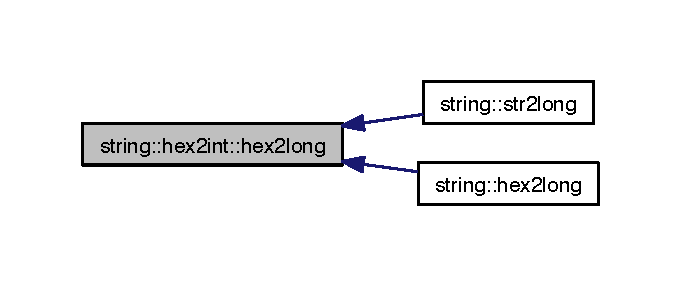
\includegraphics[width=320pt]{interfacestring_1_1hex2int_a0a901aa1d536459bdc14c2f9aba9444e_icgraph}
\end{center}
\end{figure}




The documentation for this interface was generated from the following file\+:\begin{DoxyCompactItemize}
\item 
src/\hyperlink{utils_8f90}{utils.\+f90}\end{DoxyCompactItemize}

\hypertarget{strucths__class_1_1hs}{\section{hs\+\_\+class\+:\+:hs Type Reference}
\label{strucths__class_1_1hs}\index{hs\+\_\+class\+::hs@{hs\+\_\+class\+::hs}}
}


Quantum subsystem primitive type.  


\subsection*{Private Attributes}
\begin{DoxyCompactItemize}
\item 
logical \hyperlink{strucths__class_1_1hs_a39ff1ef8fc5a20f97973d4947d518c5f}{initialized}
\begin{DoxyCompactList}\small\item\em true if hs type has been properly initialized \end{DoxyCompactList}\item 
integer(long) \hyperlink{strucths__class_1_1hs_acb57246378a120bd330012dae9a3ff38}{nstate}
\begin{DoxyCompactList}\small\item\em defines the number of quantum states. \end{DoxyCompactList}\item 
real(double) \hyperlink{strucths__class_1_1hs_aa0f4d851a33f1d195d2b6b9334cdb5d5}{eg}
\begin{DoxyCompactList}\small\item\em is the energy origin often defined to be the ground state energy. \end{DoxyCompactList}\item 
real(double) \hyperlink{strucths__class_1_1hs_a45c5cb902e23547a231a25fcd34cc621}{tol}
\begin{DoxyCompactList}\small\item\em is a vestigial parameter to be removed in later versions. \end{DoxyCompactList}\item 
real(double), dimension(\+:,\+:), \\*
pointer \hyperlink{strucths__class_1_1hs_a18f6eb65a6edae047d41c8aa5a3d9d09}{diabat}
\begin{DoxyCompactList}\small\item\em is an Nx\+N matrix containing the elements of the quantum subsystem hamiltonian in the native diabatic basis. \end{DoxyCompactList}\item 
complex(double), dimension(\+:,\+:), \\*
pointer \hyperlink{strucths__class_1_1hs_aac60f7bc14df6c4a5a1363c70b69b2db}{eigenvec}
\begin{DoxyCompactList}\small\item\em is an Nx\+N matrix containing along its columns the expansion coefficients that transform the diabatic basis into the eigen state basis of the quantum subsystem hamiltonian \end{DoxyCompactList}\item 
real(double), dimension(\+:), pointer \hyperlink{strucths__class_1_1hs_ae978013c998c123a7430209fa2797511}{eigenval}
\begin{DoxyCompactList}\small\item\em is array of length N containing the eigen vaules of the eigen states. \end{DoxyCompactList}\item 
complex(double), dimension(\+:,\+:), \\*
pointer \hyperlink{strucths__class_1_1hs_ad8d40ef9d0cb7af5e9d889f2ec05225d}{den}
\begin{DoxyCompactList}\small\item\em is an Nx\+N matrix containing the reduced density matrix of the total Hamiltonian. It describes the current state of the quantum subsystem in the diabatic basis \end{DoxyCompactList}\end{DoxyCompactItemize}


\subsection{Detailed Description}
Quantum subsystem primitive type. 

\subsection{Member Data Documentation}
\hypertarget{strucths__class_1_1hs_ad8d40ef9d0cb7af5e9d889f2ec05225d}{\index{hs\+\_\+class\+::hs@{hs\+\_\+class\+::hs}!den@{den}}
\index{den@{den}!hs\+\_\+class\+::hs@{hs\+\_\+class\+::hs}}
\subsubsection[{den}]{\setlength{\rightskip}{0pt plus 5cm}complex(double), dimension(\+:,\+:), pointer hs\+\_\+class\+::hs\+::den\hspace{0.3cm}{\ttfamily [private]}}}\label{strucths__class_1_1hs_ad8d40ef9d0cb7af5e9d889f2ec05225d}


is an Nx\+N matrix containing the reduced density matrix of the total Hamiltonian. It describes the current state of the quantum subsystem in the diabatic basis 

\hypertarget{strucths__class_1_1hs_a18f6eb65a6edae047d41c8aa5a3d9d09}{\index{hs\+\_\+class\+::hs@{hs\+\_\+class\+::hs}!diabat@{diabat}}
\index{diabat@{diabat}!hs\+\_\+class\+::hs@{hs\+\_\+class\+::hs}}
\subsubsection[{diabat}]{\setlength{\rightskip}{0pt plus 5cm}real(double), dimension(\+:,\+:), pointer hs\+\_\+class\+::hs\+::diabat\hspace{0.3cm}{\ttfamily [private]}}}\label{strucths__class_1_1hs_a18f6eb65a6edae047d41c8aa5a3d9d09}


is an Nx\+N matrix containing the elements of the quantum subsystem hamiltonian in the native diabatic basis. 

\hypertarget{strucths__class_1_1hs_aa0f4d851a33f1d195d2b6b9334cdb5d5}{\index{hs\+\_\+class\+::hs@{hs\+\_\+class\+::hs}!eg@{eg}}
\index{eg@{eg}!hs\+\_\+class\+::hs@{hs\+\_\+class\+::hs}}
\subsubsection[{eg}]{\setlength{\rightskip}{0pt plus 5cm}real(double) hs\+\_\+class\+::hs\+::eg\hspace{0.3cm}{\ttfamily [private]}}}\label{strucths__class_1_1hs_aa0f4d851a33f1d195d2b6b9334cdb5d5}


is the energy origin often defined to be the ground state energy. 

\hypertarget{strucths__class_1_1hs_ae978013c998c123a7430209fa2797511}{\index{hs\+\_\+class\+::hs@{hs\+\_\+class\+::hs}!eigenval@{eigenval}}
\index{eigenval@{eigenval}!hs\+\_\+class\+::hs@{hs\+\_\+class\+::hs}}
\subsubsection[{eigenval}]{\setlength{\rightskip}{0pt plus 5cm}real(double), dimension(\+:), pointer hs\+\_\+class\+::hs\+::eigenval\hspace{0.3cm}{\ttfamily [private]}}}\label{strucths__class_1_1hs_ae978013c998c123a7430209fa2797511}


is array of length N containing the eigen vaules of the eigen states. 

\hypertarget{strucths__class_1_1hs_aac60f7bc14df6c4a5a1363c70b69b2db}{\index{hs\+\_\+class\+::hs@{hs\+\_\+class\+::hs}!eigenvec@{eigenvec}}
\index{eigenvec@{eigenvec}!hs\+\_\+class\+::hs@{hs\+\_\+class\+::hs}}
\subsubsection[{eigenvec}]{\setlength{\rightskip}{0pt plus 5cm}complex(double), dimension(\+:,\+:), pointer hs\+\_\+class\+::hs\+::eigenvec\hspace{0.3cm}{\ttfamily [private]}}}\label{strucths__class_1_1hs_aac60f7bc14df6c4a5a1363c70b69b2db}


is an Nx\+N matrix containing along its columns the expansion coefficients that transform the diabatic basis into the eigen state basis of the quantum subsystem hamiltonian 

\hypertarget{strucths__class_1_1hs_a39ff1ef8fc5a20f97973d4947d518c5f}{\index{hs\+\_\+class\+::hs@{hs\+\_\+class\+::hs}!initialized@{initialized}}
\index{initialized@{initialized}!hs\+\_\+class\+::hs@{hs\+\_\+class\+::hs}}
\subsubsection[{initialized}]{\setlength{\rightskip}{0pt plus 5cm}logical hs\+\_\+class\+::hs\+::initialized\hspace{0.3cm}{\ttfamily [private]}}}\label{strucths__class_1_1hs_a39ff1ef8fc5a20f97973d4947d518c5f}


true if hs type has been properly initialized 

\hypertarget{strucths__class_1_1hs_acb57246378a120bd330012dae9a3ff38}{\index{hs\+\_\+class\+::hs@{hs\+\_\+class\+::hs}!nstate@{nstate}}
\index{nstate@{nstate}!hs\+\_\+class\+::hs@{hs\+\_\+class\+::hs}}
\subsubsection[{nstate}]{\setlength{\rightskip}{0pt plus 5cm}integer(long) hs\+\_\+class\+::hs\+::nstate\hspace{0.3cm}{\ttfamily [private]}}}\label{strucths__class_1_1hs_acb57246378a120bd330012dae9a3ff38}


defines the number of quantum states. 

\hypertarget{strucths__class_1_1hs_a45c5cb902e23547a231a25fcd34cc621}{\index{hs\+\_\+class\+::hs@{hs\+\_\+class\+::hs}!tol@{tol}}
\index{tol@{tol}!hs\+\_\+class\+::hs@{hs\+\_\+class\+::hs}}
\subsubsection[{tol}]{\setlength{\rightskip}{0pt plus 5cm}real(double) hs\+\_\+class\+::hs\+::tol\hspace{0.3cm}{\ttfamily [private]}}}\label{strucths__class_1_1hs_a45c5cb902e23547a231a25fcd34cc621}


is a vestigial parameter to be removed in later versions. 



The documentation for this type was generated from the following file\+:\begin{DoxyCompactItemize}
\item 
src/\hyperlink{hs_8f90}{hs.\+f90}\end{DoxyCompactItemize}

\hypertarget{classhs__class}{\section{hs\+\_\+class Module Reference}
\label{classhs__class}\index{hs\+\_\+class@{hs\+\_\+class}}
}


Quantum subsystem primitive class.  


\subsection*{Data Types}
\begin{DoxyCompactItemize}
\item 
interface \hyperlink{interfacehs__class_1_1check}{check}
\begin{DoxyCompactList}\small\item\em Check is a function that checks if the attributes of the hs type are within acceptable values. \end{DoxyCompactList}\item 
interface \hyperlink{interfacehs__class_1_1display}{display}
\begin{DoxyCompactList}\small\item\em Prints out current state of the hs type. \end{DoxyCompactList}\item 
type \hyperlink{strucths__class_1_1hs}{hs}
\begin{DoxyCompactList}\small\item\em Quantum subsystem primitive type. \end{DoxyCompactList}\item 
interface \hyperlink{interfacehs__class_1_1kill}{kill}
\begin{DoxyCompactList}\small\item\em Destroys hs type. \end{DoxyCompactList}\item 
interface \hyperlink{interfacehs__class_1_1new}{new}
\begin{DoxyCompactList}\small\item\em Creates hs type. \end{DoxyCompactList}\item 
interface \hyperlink{interfacehs__class_1_1resample}{resample}
\begin{DoxyCompactList}\small\item\em Null method. \end{DoxyCompactList}\item 
interface \hyperlink{interfacehs__class_1_1save}{save}
\begin{DoxyCompactList}\small\item\em Saves the current state of the hs type to file. \end{DoxyCompactList}\item 
interface \hyperlink{interfacehs__class_1_1update}{update}
\begin{DoxyCompactList}\small\item\em Null method. \end{DoxyCompactList}\end{DoxyCompactItemize}
\subsection*{Private Member Functions}
\begin{DoxyCompactItemize}
\item 
subroutine \hyperlink{classhs__class_a7857d1f3d6a49cfbc7d397a084a9013f}{hs\+\_\+init} (this, file)
\item 
subroutine \hyperlink{classhs__class_a1d1b34bdecfb1004bd277bf53dbd3e92}{hs\+\_\+kill} (this)
\item 
subroutine \hyperlink{classhs__class_a8a479624da65dc4f4a5cae9826487bec}{hs\+\_\+update} (this)
\item 
subroutine \hyperlink{classhs__class_abf39e51fc1d47061279287a7e328d9d4}{hs\+\_\+resample} (this)
\item 
subroutine \hyperlink{classhs__class_af457ecc48ec3ffc1c107162e546155ce}{hs\+\_\+display} (this, msg)
\item 
subroutine \hyperlink{classhs__class_a3b78604825b27d4d06a70aac14b8c538}{hs\+\_\+save} (this, file)
\item 
integer(short) function \hyperlink{classhs__class_add814b6ed9b2a64f43ea34b91ce20894}{hs\+\_\+check} (this)
\end{DoxyCompactItemize}


\subsection{Detailed Description}
Quantum subsystem primitive class. 

This class defines the quantum subsystem primitive type 

\subsection{Member Function/\+Subroutine Documentation}
\hypertarget{classhs__class_add814b6ed9b2a64f43ea34b91ce20894}{\index{hs\+\_\+class@{hs\+\_\+class}!hs\+\_\+check@{hs\+\_\+check}}
\index{hs\+\_\+check@{hs\+\_\+check}!hs\+\_\+class@{hs\+\_\+class}}
\subsubsection[{hs\+\_\+check}]{\setlength{\rightskip}{0pt plus 5cm}integer(short) function hs\+\_\+class\+::hs\+\_\+check (
\begin{DoxyParamCaption}
\item[{type({\bf hs}), intent(in)}]{this}
\end{DoxyParamCaption}
)\hspace{0.3cm}{\ttfamily [private]}}}\label{classhs__class_add814b6ed9b2a64f43ea34b91ce20894}
\hypertarget{classhs__class_af457ecc48ec3ffc1c107162e546155ce}{\index{hs\+\_\+class@{hs\+\_\+class}!hs\+\_\+display@{hs\+\_\+display}}
\index{hs\+\_\+display@{hs\+\_\+display}!hs\+\_\+class@{hs\+\_\+class}}
\subsubsection[{hs\+\_\+display}]{\setlength{\rightskip}{0pt plus 5cm}subroutine hs\+\_\+class\+::hs\+\_\+display (
\begin{DoxyParamCaption}
\item[{type({\bf hs}), intent(in)}]{this, }
\item[{character$\ast$($\ast$), intent(in), optional}]{msg}
\end{DoxyParamCaption}
)\hspace{0.3cm}{\ttfamily [private]}}}\label{classhs__class_af457ecc48ec3ffc1c107162e546155ce}
\hypertarget{classhs__class_a7857d1f3d6a49cfbc7d397a084a9013f}{\index{hs\+\_\+class@{hs\+\_\+class}!hs\+\_\+init@{hs\+\_\+init}}
\index{hs\+\_\+init@{hs\+\_\+init}!hs\+\_\+class@{hs\+\_\+class}}
\subsubsection[{hs\+\_\+init}]{\setlength{\rightskip}{0pt plus 5cm}subroutine hs\+\_\+class\+::hs\+\_\+init (
\begin{DoxyParamCaption}
\item[{type({\bf hs}), intent(inout)}]{this, }
\item[{character$\ast$($\ast$), intent(in), optional}]{file}
\end{DoxyParamCaption}
)\hspace{0.3cm}{\ttfamily [private]}}}\label{classhs__class_a7857d1f3d6a49cfbc7d397a084a9013f}


Here is the call graph for this function\+:\nopagebreak
\begin{figure}[H]
\begin{center}
\leavevmode
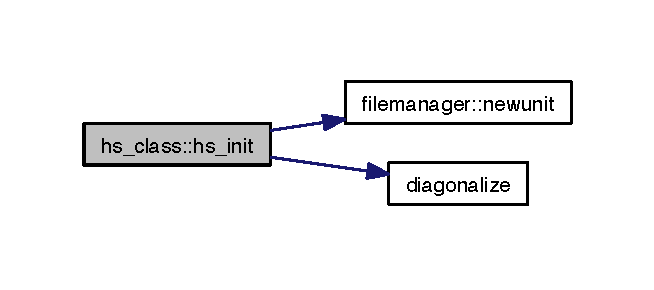
\includegraphics[width=313pt]{classhs__class_a7857d1f3d6a49cfbc7d397a084a9013f_cgraph}
\end{center}
\end{figure}


\hypertarget{classhs__class_a1d1b34bdecfb1004bd277bf53dbd3e92}{\index{hs\+\_\+class@{hs\+\_\+class}!hs\+\_\+kill@{hs\+\_\+kill}}
\index{hs\+\_\+kill@{hs\+\_\+kill}!hs\+\_\+class@{hs\+\_\+class}}
\subsubsection[{hs\+\_\+kill}]{\setlength{\rightskip}{0pt plus 5cm}subroutine hs\+\_\+class\+::hs\+\_\+kill (
\begin{DoxyParamCaption}
\item[{type({\bf hs}), intent(inout)}]{this}
\end{DoxyParamCaption}
)\hspace{0.3cm}{\ttfamily [private]}}}\label{classhs__class_a1d1b34bdecfb1004bd277bf53dbd3e92}
\hypertarget{classhs__class_abf39e51fc1d47061279287a7e328d9d4}{\index{hs\+\_\+class@{hs\+\_\+class}!hs\+\_\+resample@{hs\+\_\+resample}}
\index{hs\+\_\+resample@{hs\+\_\+resample}!hs\+\_\+class@{hs\+\_\+class}}
\subsubsection[{hs\+\_\+resample}]{\setlength{\rightskip}{0pt plus 5cm}subroutine hs\+\_\+class\+::hs\+\_\+resample (
\begin{DoxyParamCaption}
\item[{type({\bf hs}), intent(inout)}]{this}
\end{DoxyParamCaption}
)\hspace{0.3cm}{\ttfamily [private]}}}\label{classhs__class_abf39e51fc1d47061279287a7e328d9d4}


Here is the call graph for this function\+:\nopagebreak
\begin{figure}[H]
\begin{center}
\leavevmode
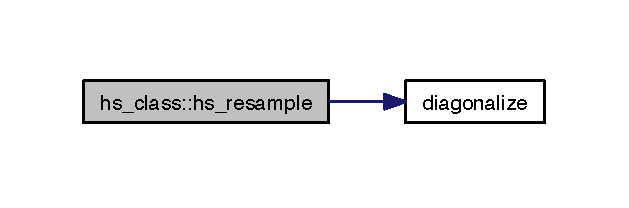
\includegraphics[width=298pt]{classhs__class_abf39e51fc1d47061279287a7e328d9d4_cgraph}
\end{center}
\end{figure}


\hypertarget{classhs__class_a3b78604825b27d4d06a70aac14b8c538}{\index{hs\+\_\+class@{hs\+\_\+class}!hs\+\_\+save@{hs\+\_\+save}}
\index{hs\+\_\+save@{hs\+\_\+save}!hs\+\_\+class@{hs\+\_\+class}}
\subsubsection[{hs\+\_\+save}]{\setlength{\rightskip}{0pt plus 5cm}subroutine hs\+\_\+class\+::hs\+\_\+save (
\begin{DoxyParamCaption}
\item[{type({\bf hs}), intent(in)}]{this, }
\item[{character$\ast$($\ast$), intent(in)}]{file}
\end{DoxyParamCaption}
)\hspace{0.3cm}{\ttfamily [private]}}}\label{classhs__class_a3b78604825b27d4d06a70aac14b8c538}


Here is the call graph for this function\+:\nopagebreak
\begin{figure}[H]
\begin{center}
\leavevmode
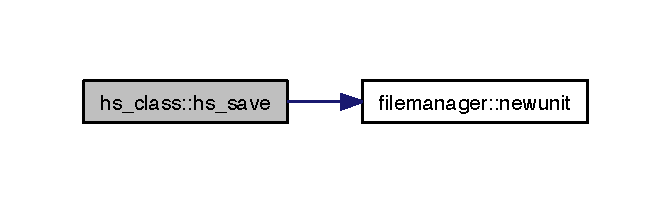
\includegraphics[width=321pt]{classhs__class_a3b78604825b27d4d06a70aac14b8c538_cgraph}
\end{center}
\end{figure}


\hypertarget{classhs__class_a8a479624da65dc4f4a5cae9826487bec}{\index{hs\+\_\+class@{hs\+\_\+class}!hs\+\_\+update@{hs\+\_\+update}}
\index{hs\+\_\+update@{hs\+\_\+update}!hs\+\_\+class@{hs\+\_\+class}}
\subsubsection[{hs\+\_\+update}]{\setlength{\rightskip}{0pt plus 5cm}subroutine hs\+\_\+class\+::hs\+\_\+update (
\begin{DoxyParamCaption}
\item[{type({\bf hs}), intent(inout)}]{this}
\end{DoxyParamCaption}
)\hspace{0.3cm}{\ttfamily [private]}}}\label{classhs__class_a8a479624da65dc4f4a5cae9826487bec}


The documentation for this module was generated from the following file\+:\begin{DoxyCompactItemize}
\item 
src/\hyperlink{hs_8f90}{hs.\+f90}\end{DoxyCompactItemize}

\hypertarget{interfacestring_1_1int2hex}{\section{string\-:\-:int2hex Interface Reference}
\label{interfacestring_1_1int2hex}\index{string\-::int2hex@{string\-::int2hex}}
}
\subsection*{Private Member Functions}
\begin{DoxyCompactItemize}
\item 
character(len=title) function \hyperlink{interfacestring_1_1int2hex_a326630b7a8f58f61d878d26307864727}{long2hex} (I)
\end{DoxyCompactItemize}


\subsection{Member Function/\-Subroutine Documentation}
\hypertarget{interfacestring_1_1int2hex_a326630b7a8f58f61d878d26307864727}{\index{string\-::int2hex@{string\-::int2hex}!long2hex@{long2hex}}
\index{long2hex@{long2hex}!string::int2hex@{string\-::int2hex}}
\subsubsection[{long2hex}]{\setlength{\rightskip}{0pt plus 5cm}character(len=title) function string\-::int2hex\-::long2hex (
\begin{DoxyParamCaption}
\item[{integer(long), intent(in)}]{I}
\end{DoxyParamCaption}
)\hspace{0.3cm}{\ttfamily [private]}}}\label{interfacestring_1_1int2hex_a326630b7a8f58f61d878d26307864727}


Here is the caller graph for this function\-:
\nopagebreak
\begin{figure}[H]
\begin{center}
\leavevmode
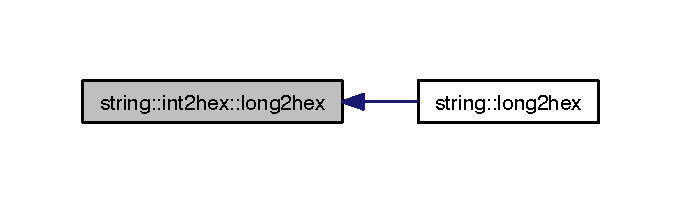
\includegraphics[width=328pt]{interfacestring_1_1int2hex_a326630b7a8f58f61d878d26307864727_icgraph}
\end{center}
\end{figure}




The documentation for this interface was generated from the following file\-:\begin{DoxyCompactItemize}
\item 
src/\hyperlink{utils_8f90}{utils.\-f90}\end{DoxyCompactItemize}

\hypertarget{interfacestring_1_1int2str}{}\section{string\+:\+:int2str Interface Reference}
\label{interfacestring_1_1int2str}\index{string\+::int2str@{string\+::int2str}}
\subsection*{Private Member Functions}
\begin{DoxyCompactItemize}
\item 
character(len=title) function \hyperlink{interfacestring_1_1int2str_a14b6077d921c2328c519b13461a07271}{long2str} (I)
\item 
character(len=title) function \hyperlink{interfacestring_1_1int2str_aa44f438a3db1b651654481ee5897c02e}{short2str} (I)
\end{DoxyCompactItemize}


\subsection{Member Function/\+Subroutine Documentation}
\mbox{\Hypertarget{interfacestring_1_1int2str_a14b6077d921c2328c519b13461a07271}\label{interfacestring_1_1int2str_a14b6077d921c2328c519b13461a07271}} 
\index{string\+::int2str@{string\+::int2str}!long2str@{long2str}}
\index{long2str@{long2str}!string\+::int2str@{string\+::int2str}}
\subsubsection{\texorpdfstring{long2str()}{long2str()}}
{\footnotesize\ttfamily character(len=title) function string\+::int2str\+::long2str (\begin{DoxyParamCaption}\item[{integer(long), intent(in)}]{I }\end{DoxyParamCaption})\hspace{0.3cm}{\ttfamily [private]}}

\mbox{\Hypertarget{interfacestring_1_1int2str_aa44f438a3db1b651654481ee5897c02e}\label{interfacestring_1_1int2str_aa44f438a3db1b651654481ee5897c02e}} 
\index{string\+::int2str@{string\+::int2str}!short2str@{short2str}}
\index{short2str@{short2str}!string\+::int2str@{string\+::int2str}}
\subsubsection{\texorpdfstring{short2str()}{short2str()}}
{\footnotesize\ttfamily character(len=title) function string\+::int2str\+::short2str (\begin{DoxyParamCaption}\item[{integer(short), intent(in)}]{I }\end{DoxyParamCaption})\hspace{0.3cm}{\ttfamily [private]}}



The documentation for this interface was generated from the following file\+:\begin{DoxyCompactItemize}
\item 
src/\hyperlink{utils_8f90}{utils.\+f90}\end{DoxyCompactItemize}

\hypertarget{interfacehs__class_1_1kill}{}\section{hs\+\_\+class\+:\+:kill Interface Reference}
\label{interfacehs__class_1_1kill}\index{hs\+\_\+class\+::kill@{hs\+\_\+class\+::kill}}


Destroys hs type.  


\subsection*{Private Member Functions}
\begin{DoxyCompactItemize}
\item 
subroutine \hyperlink{interfacehs__class_1_1kill_a812cb796d6ac4cec1ff71e473bef5cca}{hs\+\_\+kill} (this)
\end{DoxyCompactItemize}


\subsection{Detailed Description}
Destroys hs type. 

\subsection{Member Function/\+Subroutine Documentation}
\mbox{\Hypertarget{interfacehs__class_1_1kill_a812cb796d6ac4cec1ff71e473bef5cca}\label{interfacehs__class_1_1kill_a812cb796d6ac4cec1ff71e473bef5cca}} 
\index{hs\+\_\+class\+::kill@{hs\+\_\+class\+::kill}!hs\+\_\+kill@{hs\+\_\+kill}}
\index{hs\+\_\+kill@{hs\+\_\+kill}!hs\+\_\+class\+::kill@{hs\+\_\+class\+::kill}}
\subsubsection{\texorpdfstring{hs\+\_\+kill()}{hs\_kill()}}
{\footnotesize\ttfamily subroutine hs\+\_\+class\+::kill\+::hs\+\_\+kill (\begin{DoxyParamCaption}\item[{type(\hyperlink{strucths__class_1_1hs}{hs}), intent(inout)}]{this }\end{DoxyParamCaption})\hspace{0.3cm}{\ttfamily [private]}}



The documentation for this interface was generated from the following file\+:\begin{DoxyCompactItemize}
\item 
src/\hyperlink{hs_8f90}{hs.\+f90}\end{DoxyCompactItemize}

\hypertarget{interfacebilinear__class_1_1kill}{\section{bilinear\-\_\-class\-:\-:kill Interface Reference}
\label{interfacebilinear__class_1_1kill}\index{bilinear\-\_\-class\-::kill@{bilinear\-\_\-class\-::kill}}
}


Destroys the bilinear object.  


\subsection*{Private Member Functions}
\begin{DoxyCompactItemize}
\item 
subroutine \hyperlink{interfacebilinear__class_1_1kill_a13e3f18d8ff47a1f92f87642f8c9f734}{bilinear\-\_\-kill} (this)
\begin{DoxyCompactList}\small\item\em Destroys the bilinear coupling object. \end{DoxyCompactList}\end{DoxyCompactItemize}


\subsection{Detailed Description}
Destroys the bilinear object. 

\subsection{Member Function/\-Subroutine Documentation}
\hypertarget{interfacebilinear__class_1_1kill_a13e3f18d8ff47a1f92f87642f8c9f734}{\index{bilinear\-\_\-class\-::kill@{bilinear\-\_\-class\-::kill}!bilinear\-\_\-kill@{bilinear\-\_\-kill}}
\index{bilinear\-\_\-kill@{bilinear\-\_\-kill}!bilinear_class::kill@{bilinear\-\_\-class\-::kill}}
\subsubsection[{bilinear\-\_\-kill}]{\setlength{\rightskip}{0pt plus 5cm}subroutine bilinear\-\_\-class\-::kill\-::bilinear\-\_\-kill (
\begin{DoxyParamCaption}
\item[{type({\bf bilinear}), intent(inout)}]{this}
\end{DoxyParamCaption}
)\hspace{0.3cm}{\ttfamily [private]}}}\label{interfacebilinear__class_1_1kill_a13e3f18d8ff47a1f92f87642f8c9f734}


Destroys the bilinear coupling object. 


\begin{DoxyParams}{Parameters}
{\em this} & is the bilinear coupling object to be destroyed. \\
\hline
\end{DoxyParams}


The documentation for this interface was generated from the following file\-:\begin{DoxyCompactItemize}
\item 
src/\hyperlink{bilinear_8f90}{bilinear.\-f90}\end{DoxyCompactItemize}

\hypertarget{interfaceharmonicbath__class_1_1kill}{\section{harmonicbath\+\_\+class\+:\+:kill Interface Reference}
\label{interfaceharmonicbath__class_1_1kill}\index{harmonicbath\+\_\+class\+::kill@{harmonicbath\+\_\+class\+::kill}}
}
\subsection*{Private Member Functions}
\begin{DoxyCompactItemize}
\item 
subroutine \hyperlink{interfaceharmonicbath__class_1_1kill_a037b17a2340cd14c077a37329757f527}{harmonicbath\+\_\+kill} (this)
\end{DoxyCompactItemize}


\subsection{Member Function/\+Subroutine Documentation}
\hypertarget{interfaceharmonicbath__class_1_1kill_a037b17a2340cd14c077a37329757f527}{\index{harmonicbath\+\_\+class\+::kill@{harmonicbath\+\_\+class\+::kill}!harmonicbath\+\_\+kill@{harmonicbath\+\_\+kill}}
\index{harmonicbath\+\_\+kill@{harmonicbath\+\_\+kill}!harmonicbath\+\_\+class\+::kill@{harmonicbath\+\_\+class\+::kill}}
\subsubsection[{harmonicbath\+\_\+kill}]{\setlength{\rightskip}{0pt plus 5cm}subroutine harmonicbath\+\_\+class\+::kill\+::harmonicbath\+\_\+kill (
\begin{DoxyParamCaption}
\item[{type({\bf harmonicbath}), intent(inout)}]{this}
\end{DoxyParamCaption}
)\hspace{0.3cm}{\ttfamily [private]}}}\label{interfaceharmonicbath__class_1_1kill_a037b17a2340cd14c077a37329757f527}


The documentation for this interface was generated from the following file\+:\begin{DoxyCompactItemize}
\item 
src/\hyperlink{harmonicbath_8f90}{harmonicbath.\+f90}\end{DoxyCompactItemize}

\hypertarget{interfacepldm__class_1_1kill}{}\section{pldm\+\_\+class\+:\+:kill Interface Reference}
\label{interfacepldm__class_1_1kill}\index{pldm\+\_\+class\+::kill@{pldm\+\_\+class\+::kill}}
\subsection*{Private Member Functions}
\begin{DoxyCompactItemize}
\item 
subroutine \hyperlink{interfacepldm__class_1_1kill_a5c35adf2fa6446e2fa90c695a043a26a}{pldm\+\_\+kill} (this)
\end{DoxyCompactItemize}


\subsection{Member Function/\+Subroutine Documentation}
\mbox{\Hypertarget{interfacepldm__class_1_1kill_a5c35adf2fa6446e2fa90c695a043a26a}\label{interfacepldm__class_1_1kill_a5c35adf2fa6446e2fa90c695a043a26a}} 
\index{pldm\+\_\+class\+::kill@{pldm\+\_\+class\+::kill}!pldm\+\_\+kill@{pldm\+\_\+kill}}
\index{pldm\+\_\+kill@{pldm\+\_\+kill}!pldm\+\_\+class\+::kill@{pldm\+\_\+class\+::kill}}
\subsubsection{\texorpdfstring{pldm\+\_\+kill()}{pldm\_kill()}}
{\footnotesize\ttfamily subroutine pldm\+\_\+class\+::kill\+::pldm\+\_\+kill (\begin{DoxyParamCaption}\item[{type(\hyperlink{structpldm__class_1_1pldm}{pldm}), intent(inout)}]{this }\end{DoxyParamCaption})\hspace{0.3cm}{\ttfamily [private]}}



The documentation for this interface was generated from the following file\+:\begin{DoxyCompactItemize}
\item 
src/\hyperlink{_p_l_d_m_8f90}{P\+L\+D\+M.\+f90}\end{DoxyCompactItemize}

\hypertarget{interfacecoupling__class_1_1kill}{\section{coupling\-\_\-class\-:\-:kill Interface Reference}
\label{interfacecoupling__class_1_1kill}\index{coupling\-\_\-class\-::kill@{coupling\-\_\-class\-::kill}}
}
\subsection*{Private Member Functions}
\begin{DoxyCompactItemize}
\item 
subroutine \hyperlink{interfacecoupling__class_1_1kill_ae2fe896d7ad1876cf1b7a2a31afcbcdd}{coupling\-\_\-kill} (this)
\end{DoxyCompactItemize}


\subsection{Member Function/\-Subroutine Documentation}
\hypertarget{interfacecoupling__class_1_1kill_ae2fe896d7ad1876cf1b7a2a31afcbcdd}{\index{coupling\-\_\-class\-::kill@{coupling\-\_\-class\-::kill}!coupling\-\_\-kill@{coupling\-\_\-kill}}
\index{coupling\-\_\-kill@{coupling\-\_\-kill}!coupling_class::kill@{coupling\-\_\-class\-::kill}}
\subsubsection[{coupling\-\_\-kill}]{\setlength{\rightskip}{0pt plus 5cm}subroutine coupling\-\_\-class\-::kill\-::coupling\-\_\-kill (
\begin{DoxyParamCaption}
\item[{type({\bf coupling}), intent(inout)}]{this}
\end{DoxyParamCaption}
)\hspace{0.3cm}{\ttfamily [private]}}}\label{interfacecoupling__class_1_1kill_ae2fe896d7ad1876cf1b7a2a31afcbcdd}


Here is the caller graph for this function\-:
\nopagebreak
\begin{figure}[H]
\begin{center}
\leavevmode
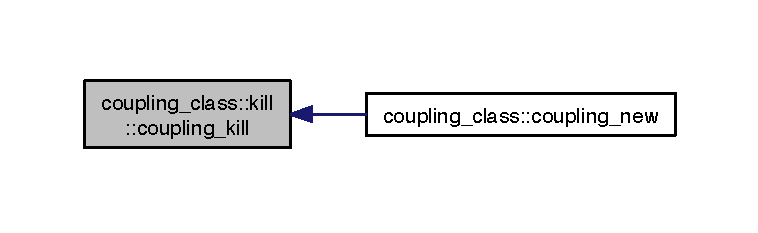
\includegraphics[width=350pt]{interfacecoupling__class_1_1kill_ae2fe896d7ad1876cf1b7a2a31afcbcdd_icgraph}
\end{center}
\end{figure}




The documentation for this interface was generated from the following file\-:\begin{DoxyCompactItemize}
\item 
src/\hyperlink{coupling_8f90}{coupling.\-f90}\end{DoxyCompactItemize}

\hypertarget{interfacetemplate__class_1_1kill}{}\section{template\+\_\+class\+:\+:kill Interface Reference}
\label{interfacetemplate__class_1_1kill}\index{template\+\_\+class\+::kill@{template\+\_\+class\+::kill}}


Destroys the T\+E\+M\+P\+L\+A\+TE object.  


\subsection*{Private Member Functions}
\begin{DoxyCompactItemize}
\item 
subroutine \hyperlink{interfacetemplate__class_1_1kill_a4a87b430982dbc5743fbdc7d82bc1092}{template\+\_\+kill} (this)
\begin{DoxyCompactList}\small\item\em Destroys the T\+E\+M\+P\+L\+A\+TE object. \end{DoxyCompactList}\end{DoxyCompactItemize}


\subsection{Detailed Description}
Destroys the T\+E\+M\+P\+L\+A\+TE object. 

\subsection{Member Function/\+Subroutine Documentation}
\mbox{\Hypertarget{interfacetemplate__class_1_1kill_a4a87b430982dbc5743fbdc7d82bc1092}\label{interfacetemplate__class_1_1kill_a4a87b430982dbc5743fbdc7d82bc1092}} 
\index{template\+\_\+class\+::kill@{template\+\_\+class\+::kill}!template\+\_\+kill@{template\+\_\+kill}}
\index{template\+\_\+kill@{template\+\_\+kill}!template\+\_\+class\+::kill@{template\+\_\+class\+::kill}}
\subsubsection{\texorpdfstring{template\+\_\+kill()}{template\_kill()}}
{\footnotesize\ttfamily subroutine template\+\_\+class\+::kill\+::template\+\_\+kill (\begin{DoxyParamCaption}\item[{type(\hyperlink{structtemplate__class_1_1template}{template}), intent(inout)}]{this }\end{DoxyParamCaption})\hspace{0.3cm}{\ttfamily [private]}}



Destroys the T\+E\+M\+P\+L\+A\+TE object. 


\begin{DoxyParams}{Parameters}
{\em this} & is the T\+E\+M\+P\+L\+A\+TE object to be destroyed. \\
\hline
\end{DoxyParams}


The documentation for this interface was generated from the following file\+:\begin{DoxyCompactItemize}
\item 
src/\hyperlink{_t_e_m_p_l_a_t_e_8f90}{T\+E\+M\+P\+L\+A\+T\+E.\+f90}\end{DoxyCompactItemize}

\hypertarget{interfacequantum__class_1_1kill}{}\section{quantum\+\_\+class\+:\+:kill Interface Reference}
\label{interfacequantum__class_1_1kill}\index{quantum\+\_\+class\+::kill@{quantum\+\_\+class\+::kill}}
\subsection*{Private Member Functions}
\begin{DoxyCompactItemize}
\item 
subroutine \hyperlink{interfacequantum__class_1_1kill_a54cb31ae4f56af89238b7a2602aab87d}{quantum\+\_\+kill} (this)
\end{DoxyCompactItemize}


\subsection{Member Function/\+Subroutine Documentation}
\mbox{\Hypertarget{interfacequantum__class_1_1kill_a54cb31ae4f56af89238b7a2602aab87d}\label{interfacequantum__class_1_1kill_a54cb31ae4f56af89238b7a2602aab87d}} 
\index{quantum\+\_\+class\+::kill@{quantum\+\_\+class\+::kill}!quantum\+\_\+kill@{quantum\+\_\+kill}}
\index{quantum\+\_\+kill@{quantum\+\_\+kill}!quantum\+\_\+class\+::kill@{quantum\+\_\+class\+::kill}}
\subsubsection{\texorpdfstring{quantum\+\_\+kill()}{quantum\_kill()}}
{\footnotesize\ttfamily subroutine quantum\+\_\+class\+::kill\+::quantum\+\_\+kill (\begin{DoxyParamCaption}\item[{type(\hyperlink{structquantum__class_1_1quantum}{quantum}), intent(inout)}]{this }\end{DoxyParamCaption})\hspace{0.3cm}{\ttfamily [private]}}



The documentation for this interface was generated from the following file\+:\begin{DoxyCompactItemize}
\item 
src/\hyperlink{quantum_8f90}{quantum.\+f90}\end{DoxyCompactItemize}

\hypertarget{interfacehb__class_1_1kill}{}\section{hb\+\_\+class\+:\+:kill Interface Reference}
\label{interfacehb__class_1_1kill}\index{hb\+\_\+class\+::kill@{hb\+\_\+class\+::kill}}
\subsection*{Private Member Functions}
\begin{DoxyCompactItemize}
\item 
subroutine \hyperlink{interfacehb__class_1_1kill_a34dd0aea3bc633b71c5b0ad0c71a8096}{hb\+\_\+kill} (this)
\end{DoxyCompactItemize}


\subsection{Member Function/\+Subroutine Documentation}
\mbox{\Hypertarget{interfacehb__class_1_1kill_a34dd0aea3bc633b71c5b0ad0c71a8096}\label{interfacehb__class_1_1kill_a34dd0aea3bc633b71c5b0ad0c71a8096}} 
\index{hb\+\_\+class\+::kill@{hb\+\_\+class\+::kill}!hb\+\_\+kill@{hb\+\_\+kill}}
\index{hb\+\_\+kill@{hb\+\_\+kill}!hb\+\_\+class\+::kill@{hb\+\_\+class\+::kill}}
\subsubsection{\texorpdfstring{hb\+\_\+kill()}{hb\_kill()}}
{\footnotesize\ttfamily subroutine hb\+\_\+class\+::kill\+::hb\+\_\+kill (\begin{DoxyParamCaption}\item[{type(\hyperlink{structhb__class_1_1hb}{hb}), intent(inout)}]{this }\end{DoxyParamCaption})\hspace{0.3cm}{\ttfamily [private]}}



The documentation for this interface was generated from the following file\+:\begin{DoxyCompactItemize}
\item 
src/\hyperlink{hb_8f90}{hb.\+f90}\end{DoxyCompactItemize}

\hypertarget{interfaceclassical__class_1_1kill}{\section{classical\-\_\-class\-:\-:kill Interface Reference}
\label{interfaceclassical__class_1_1kill}\index{classical\-\_\-class\-::kill@{classical\-\_\-class\-::kill}}
}
\subsection*{Private Member Functions}
\begin{DoxyCompactItemize}
\item 
subroutine \hyperlink{interfaceclassical__class_1_1kill_a3b424d9287e4b6c3590b13014aaa106b}{classical\-\_\-kill} (this)
\end{DoxyCompactItemize}


\subsection{Member Function/\-Subroutine Documentation}
\hypertarget{interfaceclassical__class_1_1kill_a3b424d9287e4b6c3590b13014aaa106b}{\index{classical\-\_\-class\-::kill@{classical\-\_\-class\-::kill}!classical\-\_\-kill@{classical\-\_\-kill}}
\index{classical\-\_\-kill@{classical\-\_\-kill}!classical_class::kill@{classical\-\_\-class\-::kill}}
\subsubsection[{classical\-\_\-kill}]{\setlength{\rightskip}{0pt plus 5cm}subroutine classical\-\_\-class\-::kill\-::classical\-\_\-kill (
\begin{DoxyParamCaption}
\item[{type({\bf classical}), intent(inout)}]{this}
\end{DoxyParamCaption}
)\hspace{0.3cm}{\ttfamily [private]}}}\label{interfaceclassical__class_1_1kill_a3b424d9287e4b6c3590b13014aaa106b}


Here is the caller graph for this function\-:
\nopagebreak
\begin{figure}[H]
\begin{center}
\leavevmode
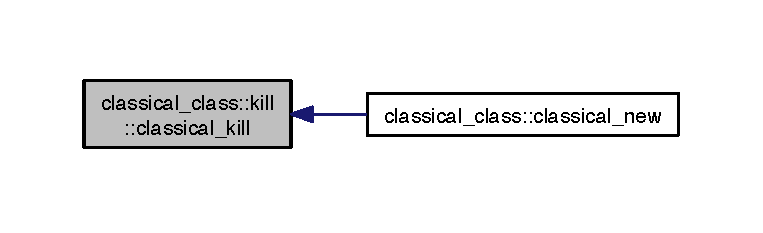
\includegraphics[width=350pt]{interfaceclassical__class_1_1kill_a3b424d9287e4b6c3590b13014aaa106b_icgraph}
\end{center}
\end{figure}




The documentation for this interface was generated from the following file\-:\begin{DoxyCompactItemize}
\item 
src/\hyperlink{classical_8f90}{classical.\-f90}\end{DoxyCompactItemize}

\hypertarget{interfacespectrometer__class_1_1kill}{\section{spectrometer\+\_\+class\+:\+:kill Interface Reference}
\label{interfacespectrometer__class_1_1kill}\index{spectrometer\+\_\+class\+::kill@{spectrometer\+\_\+class\+::kill}}
}


Destroys the spectrum type.  


\subsection*{Private Member Functions}
\begin{DoxyCompactItemize}
\item 
subroutine \hyperlink{interfacespectrometer__class_1_1kill_a260b2c75028e2be65c788d31a47b9174}{spectrum\+\_\+kill} (this)
\begin{DoxyCompactList}\small\item\em nullifies spectrum pointer \end{DoxyCompactList}\end{DoxyCompactItemize}


\subsection{Detailed Description}
Destroys the spectrum type. 

\subsection{Member Function/\+Subroutine Documentation}
\hypertarget{interfacespectrometer__class_1_1kill_a260b2c75028e2be65c788d31a47b9174}{\index{spectrometer\+\_\+class\+::kill@{spectrometer\+\_\+class\+::kill}!spectrum\+\_\+kill@{spectrum\+\_\+kill}}
\index{spectrum\+\_\+kill@{spectrum\+\_\+kill}!spectrometer\+\_\+class\+::kill@{spectrometer\+\_\+class\+::kill}}
\subsubsection[{spectrum\+\_\+kill}]{\setlength{\rightskip}{0pt plus 5cm}subroutine spectrometer\+\_\+class\+::kill\+::spectrum\+\_\+kill (
\begin{DoxyParamCaption}
\item[{type({\bf spectrum}), intent(inout)}]{this}
\end{DoxyParamCaption}
)\hspace{0.3cm}{\ttfamily [private]}}}\label{interfacespectrometer__class_1_1kill_a260b2c75028e2be65c788d31a47b9174}


nullifies spectrum pointer 


\begin{DoxyParams}[1]{Parameters}
\mbox{\tt in,out}  & {\em this} & spectrum type \\
\hline
\end{DoxyParams}


The documentation for this interface was generated from the following file\+:\begin{DoxyCompactItemize}
\item 
src/\hyperlink{spectrometer_8f90}{spectrometer.\+f90}\end{DoxyCompactItemize}

\hypertarget{interfacehc__class_1_1kill}{\section{hc\-\_\-class\-:\-:kill Interface Reference}
\label{interfacehc__class_1_1kill}\index{hc\-\_\-class\-::kill@{hc\-\_\-class\-::kill}}
}
\subsection*{Private Member Functions}
\begin{DoxyCompactItemize}
\item 
subroutine \hyperlink{interfacehc__class_1_1kill_a05e977cf47d5345bb6b255b3bf85eb89}{hc\-\_\-kill} (this)
\end{DoxyCompactItemize}


\subsection{Member Function/\-Subroutine Documentation}
\hypertarget{interfacehc__class_1_1kill_a05e977cf47d5345bb6b255b3bf85eb89}{\index{hc\-\_\-class\-::kill@{hc\-\_\-class\-::kill}!hc\-\_\-kill@{hc\-\_\-kill}}
\index{hc\-\_\-kill@{hc\-\_\-kill}!hc_class::kill@{hc\-\_\-class\-::kill}}
\subsubsection[{hc\-\_\-kill}]{\setlength{\rightskip}{0pt plus 5cm}subroutine hc\-\_\-class\-::kill\-::hc\-\_\-kill (
\begin{DoxyParamCaption}
\item[{type({\bf hc}), intent(inout)}]{this}
\end{DoxyParamCaption}
)\hspace{0.3cm}{\ttfamily [private]}}}\label{interfacehc__class_1_1kill_a05e977cf47d5345bb6b255b3bf85eb89}


The documentation for this interface was generated from the following file\-:\begin{DoxyCompactItemize}
\item 
src/\hyperlink{hc_8f90}{hc.\-f90}\end{DoxyCompactItemize}

\hypertarget{interfacedipoles__class_1_1kill}{}\section{dipoles\+\_\+class\+:\+:kill Interface Reference}
\label{interfacedipoles__class_1_1kill}\index{dipoles\+\_\+class\+::kill@{dipoles\+\_\+class\+::kill}}
\subsection*{Private Member Functions}
\begin{DoxyCompactItemize}
\item 
subroutine \hyperlink{interfacedipoles__class_1_1kill_a0dacd933f05d84b7752ed570857ffedc}{dipoles\+\_\+kill} (this)
\end{DoxyCompactItemize}


\subsection{Member Function/\+Subroutine Documentation}
\mbox{\Hypertarget{interfacedipoles__class_1_1kill_a0dacd933f05d84b7752ed570857ffedc}\label{interfacedipoles__class_1_1kill_a0dacd933f05d84b7752ed570857ffedc}} 
\index{dipoles\+\_\+class\+::kill@{dipoles\+\_\+class\+::kill}!dipoles\+\_\+kill@{dipoles\+\_\+kill}}
\index{dipoles\+\_\+kill@{dipoles\+\_\+kill}!dipoles\+\_\+class\+::kill@{dipoles\+\_\+class\+::kill}}
\subsubsection{\texorpdfstring{dipoles\+\_\+kill()}{dipoles\_kill()}}
{\footnotesize\ttfamily subroutine dipoles\+\_\+class\+::kill\+::dipoles\+\_\+kill (\begin{DoxyParamCaption}\item[{type(\hyperlink{structdipoles__class_1_1dipoles}{dipoles}), intent(inout)}]{this }\end{DoxyParamCaption})\hspace{0.3cm}{\ttfamily [private]}}



The documentation for this interface was generated from the following file\+:\begin{DoxyCompactItemize}
\item 
src/\hyperlink{dipoles_8f90}{dipoles.\+f90}\end{DoxyCompactItemize}

\hypertarget{classmath}{\section{math Module Reference}
\label{classmath}\index{math@{math}}
}


Definition of mathematical constants and operators.  


\subsection*{Public Member Functions}
\begin{DoxyCompactItemize}
\item 
real(double) function, \\*
dimension(n, n), public \hyperlink{classmath_a43efec08acf55747fa1e14085858aade}{iden} (N)
\begin{DoxyCompactList}\small\item\em identity matrix \end{DoxyCompactList}\item 
real(double) function, public \hyperlink{classmath_a9f8f22c01066f03fe5900edb63b56c89}{trace} (A)
\begin{DoxyCompactList}\small\item\em trace of a complex matrix \end{DoxyCompactList}\item 
real(double) function, public \hyperlink{classmath_a864984937cf0f3b7bdbc9b652b84445d}{cnorm} (A)
\begin{DoxyCompactList}\small\item\em Entrywise p-\/norm of a complex square matrix with p=1. \end{DoxyCompactList}\item 
real(double) function, public \hyperlink{classmath_a2830cb5393b6e6a8baa8d072c73ce8a9}{fnorm} (A, p)
\begin{DoxyCompactList}\small\item\em Entrywise p-\/norm of a complex matrix. \end{DoxyCompactList}\end{DoxyCompactItemize}
\subsection*{Public Attributes}
\begin{DoxyCompactItemize}
\item 
real(double), parameter \hyperlink{classmath_aa2f838077707f6cdb0c8a0ec69719690}{pi}
\item 
real(double), parameter \hyperlink{classmath_aeb6d7ed6a20444e26f024b34eaa4c4f7}{twopi}
\item 
real(double), parameter \hyperlink{classmath_a83cddb754967ada1a15217d10ed9c24b}{fourpi}
\item 
real(double), parameter \hyperlink{classmath_a99d72d3bce2cadc8630d10ee09aaa3ea}{halfpi}
\item 
complex(double), parameter \hyperlink{classmath_ae0354610846d49064ea0336f19d5bf3f}{eye}
\end{DoxyCompactItemize}


\subsection{Detailed Description}
Definition of mathematical constants and operators. 

\begin{DoxyAuthor}{Authors}
Author\+: Daniel Montemayor 
\end{DoxyAuthor}
\begin{DoxyRefDesc}{Todo}
\item[\hyperlink{todo__todo000014}{Todo}]
\begin{DoxyItemize}
\item Add cross and dot product operators 
\end{DoxyItemize}\end{DoxyRefDesc}


\subsection{Member Function/\+Subroutine Documentation}
\hypertarget{classmath_a864984937cf0f3b7bdbc9b652b84445d}{\index{math@{math}!cnorm@{cnorm}}
\index{cnorm@{cnorm}!math@{math}}
\subsubsection[{cnorm}]{\setlength{\rightskip}{0pt plus 5cm}real(double) function, public math\+::cnorm (
\begin{DoxyParamCaption}
\item[{complex(double), dimension(\+:,\+:), intent(in)}]{A}
\end{DoxyParamCaption}
)}}\label{classmath_a864984937cf0f3b7bdbc9b652b84445d}


Entrywise p-\/norm of a complex square matrix with p=1. 


\begin{DoxyParams}[1]{Parameters}
\mbox{\tt in}  & {\em A} & matrix $<$ \\
\hline
\end{DoxyParams}


Here is the caller graph for this function\+:\nopagebreak
\begin{figure}[H]
\begin{center}
\leavevmode
\includegraphics[width=350pt]{classmath_a864984937cf0f3b7bdbc9b652b84445d_icgraph}
\end{center}
\end{figure}


\hypertarget{classmath_a2830cb5393b6e6a8baa8d072c73ce8a9}{\index{math@{math}!fnorm@{fnorm}}
\index{fnorm@{fnorm}!math@{math}}
\subsubsection[{fnorm}]{\setlength{\rightskip}{0pt plus 5cm}real(double) function, public math\+::fnorm (
\begin{DoxyParamCaption}
\item[{complex(double), dimension(\+:,\+:), intent(in)}]{A, }
\item[{integer(long), intent(in), optional}]{p}
\end{DoxyParamCaption}
)}}\label{classmath_a2830cb5393b6e6a8baa8d072c73ce8a9}


Entrywise p-\/norm of a complex matrix. 


\begin{DoxyParams}[1]{Parameters}
\mbox{\tt in}  & {\em A} & matrix \\
\hline
\mbox{\tt in}  & {\em p} & optional p-\/norm integer default\+: p=2 Frobinius normalization $<$ \\
\hline
\end{DoxyParams}
\hypertarget{classmath_a43efec08acf55747fa1e14085858aade}{\index{math@{math}!iden@{iden}}
\index{iden@{iden}!math@{math}}
\subsubsection[{iden}]{\setlength{\rightskip}{0pt plus 5cm}real(double) function, dimension(n,n), public math\+::iden (
\begin{DoxyParamCaption}
\item[{integer(long), intent(in)}]{N}
\end{DoxyParamCaption}
)}}\label{classmath_a43efec08acf55747fa1e14085858aade}


identity matrix 


\begin{DoxyParams}[1]{Parameters}
\mbox{\tt in}  & {\em N} & size of matrix $<$ \\
\hline
\end{DoxyParams}


Here is the caller graph for this function\+:\nopagebreak
\begin{figure}[H]
\begin{center}
\leavevmode
\includegraphics[width=328pt]{classmath_a43efec08acf55747fa1e14085858aade_icgraph}
\end{center}
\end{figure}


\hypertarget{classmath_a9f8f22c01066f03fe5900edb63b56c89}{\index{math@{math}!trace@{trace}}
\index{trace@{trace}!math@{math}}
\subsubsection[{trace}]{\setlength{\rightskip}{0pt plus 5cm}real(double) function, public math\+::trace (
\begin{DoxyParamCaption}
\item[{complex(double), dimension(\+:,\+:), intent(in)}]{A}
\end{DoxyParamCaption}
)}}\label{classmath_a9f8f22c01066f03fe5900edb63b56c89}


trace of a complex matrix 


\begin{DoxyParams}[1]{Parameters}
\mbox{\tt in}  & {\em A} & matrix $<$ \\
\hline
\end{DoxyParams}


Here is the caller graph for this function\+:\nopagebreak
\begin{figure}[H]
\begin{center}
\leavevmode
\includegraphics[width=294pt]{classmath_a9f8f22c01066f03fe5900edb63b56c89_icgraph}
\end{center}
\end{figure}




\subsection{Member Data Documentation}
\hypertarget{classmath_ae0354610846d49064ea0336f19d5bf3f}{\index{math@{math}!eye@{eye}}
\index{eye@{eye}!math@{math}}
\subsubsection[{eye}]{\setlength{\rightskip}{0pt plus 5cm}complex(double), parameter math\+::eye}}\label{classmath_ae0354610846d49064ea0336f19d5bf3f}
\hypertarget{classmath_a83cddb754967ada1a15217d10ed9c24b}{\index{math@{math}!fourpi@{fourpi}}
\index{fourpi@{fourpi}!math@{math}}
\subsubsection[{fourpi}]{\setlength{\rightskip}{0pt plus 5cm}real(double), parameter math\+::fourpi}}\label{classmath_a83cddb754967ada1a15217d10ed9c24b}
\hypertarget{classmath_a99d72d3bce2cadc8630d10ee09aaa3ea}{\index{math@{math}!halfpi@{halfpi}}
\index{halfpi@{halfpi}!math@{math}}
\subsubsection[{halfpi}]{\setlength{\rightskip}{0pt plus 5cm}real(double), parameter math\+::halfpi}}\label{classmath_a99d72d3bce2cadc8630d10ee09aaa3ea}
\hypertarget{classmath_aa2f838077707f6cdb0c8a0ec69719690}{\index{math@{math}!pi@{pi}}
\index{pi@{pi}!math@{math}}
\subsubsection[{pi}]{\setlength{\rightskip}{0pt plus 5cm}real(double), parameter math\+::pi}}\label{classmath_aa2f838077707f6cdb0c8a0ec69719690}
\hypertarget{classmath_aeb6d7ed6a20444e26f024b34eaa4c4f7}{\index{math@{math}!twopi@{twopi}}
\index{twopi@{twopi}!math@{math}}
\subsubsection[{twopi}]{\setlength{\rightskip}{0pt plus 5cm}real(double), parameter math\+::twopi}}\label{classmath_aeb6d7ed6a20444e26f024b34eaa4c4f7}


The documentation for this module was generated from the following file\+:\begin{DoxyCompactItemize}
\item 
src/\hyperlink{utils_8f90}{utils.\+f90}\end{DoxyCompactItemize}

\hypertarget{structmolreader_1_1model}{}\section{molreader\+:\+:model Type Reference}
\label{structmolreader_1_1model}\index{molreader\+::model@{molreader\+::model}}
\subsection*{Private Attributes}
\begin{DoxyCompactItemize}
\item 
character(len=11) \hyperlink{structmolreader_1_1model_a23b8930632b27e87549d8b297f827fd6}{fmt}
\item 
character(len=\hyperlink{namespacemolreader_a8f12be3272b946fd698c9fbaf2ba9d32}{reclen}) \hyperlink{structmolreader_1_1model_abac2ce11a9e639f8e2c4b29e40e87298}{recname}
\item 
integer(long) \hyperlink{structmolreader_1_1model_aff0c60ac8af22248ab65fa453bf87e6a}{serial}
\end{DoxyCompactItemize}


\subsection{Member Data Documentation}
\mbox{\Hypertarget{structmolreader_1_1model_a23b8930632b27e87549d8b297f827fd6}\label{structmolreader_1_1model_a23b8930632b27e87549d8b297f827fd6}} 
\index{molreader\+::model@{molreader\+::model}!fmt@{fmt}}
\index{fmt@{fmt}!molreader\+::model@{molreader\+::model}}
\subsubsection{\texorpdfstring{fmt}{fmt}}
{\footnotesize\ttfamily character(len=11) molreader\+::model\+::fmt\hspace{0.3cm}{\ttfamily [private]}}

\mbox{\Hypertarget{structmolreader_1_1model_abac2ce11a9e639f8e2c4b29e40e87298}\label{structmolreader_1_1model_abac2ce11a9e639f8e2c4b29e40e87298}} 
\index{molreader\+::model@{molreader\+::model}!recname@{recname}}
\index{recname@{recname}!molreader\+::model@{molreader\+::model}}
\subsubsection{\texorpdfstring{recname}{recname}}
{\footnotesize\ttfamily character(len=\hyperlink{namespacemolreader_a8f12be3272b946fd698c9fbaf2ba9d32}{reclen}) molreader\+::model\+::recname\hspace{0.3cm}{\ttfamily [private]}}

\mbox{\Hypertarget{structmolreader_1_1model_aff0c60ac8af22248ab65fa453bf87e6a}\label{structmolreader_1_1model_aff0c60ac8af22248ab65fa453bf87e6a}} 
\index{molreader\+::model@{molreader\+::model}!serial@{serial}}
\index{serial@{serial}!molreader\+::model@{molreader\+::model}}
\subsubsection{\texorpdfstring{serial}{serial}}
{\footnotesize\ttfamily integer(long) molreader\+::model\+::serial\hspace{0.3cm}{\ttfamily [private]}}



The documentation for this type was generated from the following file\+:\begin{DoxyCompactItemize}
\item 
src/\hyperlink{molreader_8f90}{molreader.\+f90}\end{DoxyCompactItemize}

\hypertarget{classmolreader}{\section{molreader Module Reference}
\label{classmolreader}\index{molreader@{molreader}}
}


Molecule Building Utility.  


\subsection*{Data Types}
\begin{DoxyCompactItemize}
\item 
interface \hyperlink{interfacemolreader_1_1advance__record}{advance\-\_\-record}
\item 
type \hyperlink{structmolreader_1_1atom}{atom}
\item 
type \hyperlink{structmolreader_1_1cryst1}{cryst1}
\item 
interface \hyperlink{interfacemolreader_1_1display}{display}
\item 
type \hyperlink{structmolreader_1_1model}{model}
\item 
interface \hyperlink{interfacemolreader_1_1new}{new}
\item 
type \hyperlink{structmolreader_1_1psfatom}{psfatom}
\item 
interface \hyperlink{interfacemolreader_1_1read}{read}
\end{DoxyCompactItemize}
\subsection*{Public Member Functions}
\begin{DoxyCompactItemize}
\item 
character(len=\hyperlink{classmolreader_a8f12be3272b946fd698c9fbaf2ba9d32}{reclen}) function, \\*
public \hyperlink{classmolreader_af6c857ef51f99971a66b1c293d24906b}{next\-\_\-record} ()
\item 
subroutine, public \hyperlink{classmolreader_a38a3903d901bc5e0b318bcc0dfd1b3ff}{open\-\_\-pdb} (file)
\begin{DoxyCompactList}\small\item\em Initialize P\-D\-B file for parsing. \end{DoxyCompactList}\item 
subroutine, public \hyperlink{classmolreader_a5aafbdb9b4afbb96bdc20ae58d547699}{close\-\_\-pdb}
\item 
subroutine, public \hyperlink{classmolreader_af85c66302e278af03e0cc94dc42e662e}{rewind\-\_\-pdb}
\begin{DoxyCompactList}\small\item\em Rewind an initialized P\-D\-B file for parsing. \end{DoxyCompactList}\item 
character(len=\hyperlink{classmolreader_acd493d996a1fcd0ed77937e925c9b7fe}{linelen}) \\*
function, public \hyperlink{classmolreader_ac6b85a406b7ebd0810f0d63beeeda783}{next\-\_\-psf} ()
\item 
subroutine, public \hyperlink{classmolreader_a3ebd81391f00e3279bf262b2879af97a}{open\-\_\-psf} (file)
\begin{DoxyCompactList}\small\item\em Initialize P\-S\-F file for parsing. \end{DoxyCompactList}\item 
subroutine, public \hyperlink{classmolreader_aac446b95d6c274d93e11e45286e60e4d}{close\-\_\-psf}
\item 
subroutine, public \hyperlink{classmolreader_a6d79c8d97fd91cfb25dec2b67320c77b}{rewind\-\_\-psf}
\begin{DoxyCompactList}\small\item\em Rewind an initialized P\-S\-F file for parsing. \end{DoxyCompactList}\item 
subroutine, public \hyperlink{classmolreader_a7a4cb6436916cd4b8ee0341d528e9c73}{advance\-\_\-psf} (section, nrecord)
\begin{DoxyCompactList}\small\item\em Advances opened psf file. \end{DoxyCompactList}\end{DoxyCompactItemize}
\subsection*{Private Member Functions}
\begin{DoxyCompactItemize}
\item 
subroutine \hyperlink{classmolreader_af85c1b386f0dc78ebf55e003b4f8c83a}{read\-\_\-cryst1} (this)
\item 
subroutine \hyperlink{classmolreader_ac9a2b0ff287faa780311cc432b866610}{display\-\_\-cryst1} (this, unit)
\item 
subroutine \hyperlink{classmolreader_ac284dc33f40874d6156c1cd36781002c}{new\-\_\-cryst1} (this)
\item 
subroutine \hyperlink{classmolreader_a64ff990dc05c01debc1138dd012f4bcb}{read\-\_\-model} (this)
\begin{DoxyCompactList}\small\item\em Reads and returns M\-O\-D\-E\-L Record type. \end{DoxyCompactList}\item 
subroutine \hyperlink{classmolreader_a462d061944b74f7145b8bf89fc3439fc}{display\-\_\-model} (this, unit)
\item 
subroutine \hyperlink{classmolreader_a8edb660b2e1b64a5d78593c734afbe95}{new\-\_\-model} (this)
\item 
subroutine \hyperlink{classmolreader_a49ccaf345b633e27f69ad7a5a8637a2a}{read\-\_\-atom} (this)
\begin{DoxyCompactList}\small\item\em Reads and returns A\-T\-O\-M/\-H\-E\-T\-A\-T\-M/\-T\-E\-R Record types. \end{DoxyCompactList}\item 
subroutine \hyperlink{classmolreader_ae1000e1ea4e46f858a3640c08563c3ff}{new\-\_\-atom} (this)
\item 
subroutine \hyperlink{classmolreader_adb757da4ec2256578422254dad5b262e}{display\-\_\-atom} (this, unit)
\item 
subroutine \hyperlink{classmolreader_a16d4776fded57cf8aa38f639610cad84}{refresh\-\_\-buffer}
\item 
subroutine \hyperlink{classmolreader_ac7b950f165e89b12ccc8fff1c0f3bae9}{advance\-\_\-buffer}
\item 
subroutine \hyperlink{classmolreader_a81fcc5a3f49380ccd10b02b229f5067d}{read\-\_\-psfatom} (this)
\item 
subroutine \hyperlink{classmolreader_a737dbe023a6cbecab8269981ffdfa31c}{display\-\_\-psfatom} (this, unit)
\item 
subroutine \hyperlink{classmolreader_a56968311293e3c68022fe3bbe3600306}{new\-\_\-psfatom} (this)
\item 
subroutine \hyperlink{classmolreader_abf243c87d2f9429f3ed94293d438c7c7}{advance\-\_\-psfbuffer}
\item 
subroutine \hyperlink{classmolreader_a13131c46b34d0385ba7eadd0b1b88df9}{refresh\-\_\-psfbuffer}
\end{DoxyCompactItemize}
\subsection*{Private Attributes}
\begin{DoxyCompactItemize}
\item 
integer(long) \hyperlink{classmolreader_a5b0570862e5318937ea68a01966ed56f}{pdbunit}
\item 
integer(long) \hyperlink{classmolreader_a2b57a032db6161c98961f5e8109c3b90}{psfunit}
\item 
integer(long) \hyperlink{classmolreader_ac41219b2f68591f315dded4488483263}{parsingunit}
\item 
character(len=path) \hyperlink{classmolreader_aa372f060e4e581b1c14e2b46a65d2df4}{pdbfile}
\item 
character(len=path) \hyperlink{classmolreader_a48ac5c969e35417342bb66a57adec842}{psffile}
\item 
logical \hyperlink{classmolreader_ad7636360c8e0ecb526000567dd32d2d0}{pdbisopen}
\item 
logical \hyperlink{classmolreader_ae5cd9063d12a39b0e8266e184439c808}{psfisopen}
\item 
integer(long), parameter \hyperlink{classmolreader_a8f12be3272b946fd698c9fbaf2ba9d32}{reclen}
\item 
integer(long), parameter \hyperlink{classmolreader_acd493d996a1fcd0ed77937e925c9b7fe}{linelen}
\item 
integer(long), parameter \hyperlink{classmolreader_a7192fdfba4bcb0ee7504a9c6695c7106}{maxrecord}
\item 
character(len=5) \hyperlink{classmolreader_ac14650c697f68fd15530b93807e3f42f}{linefmt}
\item 
character(len=\hyperlink{classmolreader_acd493d996a1fcd0ed77937e925c9b7fe}{linelen}), \\*
dimension(\hyperlink{classmolreader_a7192fdfba4bcb0ee7504a9c6695c7106}{maxrecord}) \hyperlink{classmolreader_a06d78b69405420664607fb01b4d8e97a}{buffer}
\item 
character(len=\hyperlink{classmolreader_acd493d996a1fcd0ed77937e925c9b7fe}{linelen}), \\*
dimension(\hyperlink{classmolreader_a7192fdfba4bcb0ee7504a9c6695c7106}{maxrecord}) \hyperlink{classmolreader_aab845daa54f6803a37ceb91d7ad296a7}{psfbuffer}
\item 
integer(long) \hyperlink{classmolreader_a7b2e4f11efe55d80469efa3f7aeacbab}{buffer\-\_\-cursor}
\item 
integer(long) \hyperlink{classmolreader_ac7969154d301aab4a51cde89ec2f08ee}{buffer\-\_\-count}
\item 
integer(long) \hyperlink{classmolreader_ab080c636a2423beb139bdd65dcd884c3}{psfbuffer\-\_\-cursor}
\item 
integer(long) \hyperlink{classmolreader_af2dddaa7f6249a39287ffcdcbe2ce558}{psfbuffer\-\_\-count}
\item 
logical, dimension(\hyperlink{classmolreader_a7192fdfba4bcb0ee7504a9c6695c7106}{maxrecord}) \hyperlink{classmolreader_a3368bfc7f2d07a7f472a8118220516a9}{buffermask}
\item 
logical, dimension(\hyperlink{classmolreader_a7192fdfba4bcb0ee7504a9c6695c7106}{maxrecord}) \hyperlink{classmolreader_a747bd2c32990916c313506c805317e88}{psfbuffermask}
\item 
logical \hyperlink{classmolreader_a1f82d6f3302ab89b43d1fcbcba5d8fb2}{recording\-\_\-parsingdata}
\item 
logical \hyperlink{classmolreader_aec460f295b88cb8eb8dd58901edce0ba}{to}
\item 
logical \hyperlink{classmolreader_af3ae5caa4d00fa50c74d2f3154e8ea7c}{save}
\item 
logical \hyperlink{classmolreader_a151a8b8c33b86ab86d352aeaaf9ec84b}{parsing}
\item 
logical \hyperlink{classmolreader_a29899cd9778ac12af6bad404c1092518}{timing}
\item 
logical \hyperlink{classmolreader_ad29941441961d6bb225120cc88f93db7}{data}
\item 
real(double) \hyperlink{classmolreader_a5cf7dc5ccdeb068704a693ec6b248796}{parsing\-\_\-rate}
\item 
real(double) \hyperlink{classmolreader_ad5b1ed6898caa1c2161f0cdc6c10fc72}{time0}
\end{DoxyCompactItemize}


\subsection{Detailed Description}
Molecule Building Utility. 

Supports P\-D\-B -\/ Atomic Coordinate Entry Format Version 3.\-3 plus some extra P\-D\-B entries typical of some M\-D packages. \begin{DoxyAuthor}{Authors}
Daniel Montemayor 
\end{DoxyAuthor}
\begin{DoxyDate}{Date}
23 Feb 2012 
\end{DoxyDate}
\begin{DoxyRefDesc}{Bug}
\item[\hyperlink{bug__bug000001}{Bug}]psf file cannont have extra charaters in 'section' line. (go to advance\-\_\-psf subrtouine) \end{DoxyRefDesc}
\begin{DoxyRefDesc}{Todo}
\item[\hyperlink{todo__todo000002}{Todo}]depreciate next\-\_\-record, and \hyperlink{interfacemolreader_1_1advance__record}{advance\-\_\-record} use instead next\-\_\-pdb and advance\-\_\-pdb \end{DoxyRefDesc}


\subsection{Member Function/\-Subroutine Documentation}
\hypertarget{classmolreader_ac7b950f165e89b12ccc8fff1c0f3bae9}{\index{molreader@{molreader}!advance\-\_\-buffer@{advance\-\_\-buffer}}
\index{advance\-\_\-buffer@{advance\-\_\-buffer}!molreader@{molreader}}
\subsubsection[{advance\-\_\-buffer}]{\setlength{\rightskip}{0pt plus 5cm}subroutine molreader\-::advance\-\_\-buffer (
\begin{DoxyParamCaption}
{}
\end{DoxyParamCaption}
)\hspace{0.3cm}{\ttfamily [private]}}}\label{classmolreader_ac7b950f165e89b12ccc8fff1c0f3bae9}


Here is the call graph for this function\-:
\nopagebreak
\begin{figure}[H]
\begin{center}
\leavevmode
\includegraphics[width=350pt]{classmolreader_ac7b950f165e89b12ccc8fff1c0f3bae9_cgraph}
\end{center}
\end{figure}


\hypertarget{classmolreader_a7a4cb6436916cd4b8ee0341d528e9c73}{\index{molreader@{molreader}!advance\-\_\-psf@{advance\-\_\-psf}}
\index{advance\-\_\-psf@{advance\-\_\-psf}!molreader@{molreader}}
\subsubsection[{advance\-\_\-psf}]{\setlength{\rightskip}{0pt plus 5cm}subroutine, public molreader\-::advance\-\_\-psf (
\begin{DoxyParamCaption}
\item[{character$\ast$($\ast$), intent(in), optional}]{section, }
\item[{integer(long), optional}]{nrecord}
\end{DoxyParamCaption}
)}}\label{classmolreader_a7a4cb6436916cd4b8ee0341d528e9c73}


Advances opened psf file. 

Advances one line or optionally to one of the following sections\-: title, atoms, bonds, angles, dihedrals, impropers, or cross-\/terms \begin{DoxyRefDesc}{Bug}
\item[\hyperlink{bug__bug000002}{Bug}]trim(str).ne.'section'\-: means that nothing else can be written on section line, the bug can be fixed by selecting the columns of the \hyperlink{classmolreader_ac6b85a406b7ebd0810f0d63beeeda783}{next\-\_\-psf()} string not the trim. \end{DoxyRefDesc}


Here is the call graph for this function\-:
\nopagebreak
\begin{figure}[H]
\begin{center}
\leavevmode
\includegraphics[width=350pt]{classmolreader_a7a4cb6436916cd4b8ee0341d528e9c73_cgraph}
\end{center}
\end{figure}


\hypertarget{classmolreader_abf243c87d2f9429f3ed94293d438c7c7}{\index{molreader@{molreader}!advance\-\_\-psfbuffer@{advance\-\_\-psfbuffer}}
\index{advance\-\_\-psfbuffer@{advance\-\_\-psfbuffer}!molreader@{molreader}}
\subsubsection[{advance\-\_\-psfbuffer}]{\setlength{\rightskip}{0pt plus 5cm}subroutine molreader\-::advance\-\_\-psfbuffer (
\begin{DoxyParamCaption}
{}
\end{DoxyParamCaption}
)\hspace{0.3cm}{\ttfamily [private]}}}\label{classmolreader_abf243c87d2f9429f3ed94293d438c7c7}


Here is the call graph for this function\-:
\nopagebreak
\begin{figure}[H]
\begin{center}
\leavevmode
\includegraphics[width=318pt]{classmolreader_abf243c87d2f9429f3ed94293d438c7c7_cgraph}
\end{center}
\end{figure}




Here is the caller graph for this function\-:
\nopagebreak
\begin{figure}[H]
\begin{center}
\leavevmode
\includegraphics[width=348pt]{classmolreader_abf243c87d2f9429f3ed94293d438c7c7_icgraph}
\end{center}
\end{figure}


\hypertarget{classmolreader_a5aafbdb9b4afbb96bdc20ae58d547699}{\index{molreader@{molreader}!close\-\_\-pdb@{close\-\_\-pdb}}
\index{close\-\_\-pdb@{close\-\_\-pdb}!molreader@{molreader}}
\subsubsection[{close\-\_\-pdb}]{\setlength{\rightskip}{0pt plus 5cm}subroutine, public molreader\-::close\-\_\-pdb (
\begin{DoxyParamCaption}
{}
\end{DoxyParamCaption}
)}}\label{classmolreader_a5aafbdb9b4afbb96bdc20ae58d547699}
\hypertarget{classmolreader_aac446b95d6c274d93e11e45286e60e4d}{\index{molreader@{molreader}!close\-\_\-psf@{close\-\_\-psf}}
\index{close\-\_\-psf@{close\-\_\-psf}!molreader@{molreader}}
\subsubsection[{close\-\_\-psf}]{\setlength{\rightskip}{0pt plus 5cm}subroutine, public molreader\-::close\-\_\-psf (
\begin{DoxyParamCaption}
{}
\end{DoxyParamCaption}
)}}\label{classmolreader_aac446b95d6c274d93e11e45286e60e4d}


Here is the caller graph for this function\-:
\nopagebreak
\begin{figure}[H]
\begin{center}
\leavevmode
\includegraphics[width=350pt]{classmolreader_aac446b95d6c274d93e11e45286e60e4d_icgraph}
\end{center}
\end{figure}


\hypertarget{classmolreader_adb757da4ec2256578422254dad5b262e}{\index{molreader@{molreader}!display\-\_\-atom@{display\-\_\-atom}}
\index{display\-\_\-atom@{display\-\_\-atom}!molreader@{molreader}}
\subsubsection[{display\-\_\-atom}]{\setlength{\rightskip}{0pt plus 5cm}subroutine molreader\-::display\-\_\-atom (
\begin{DoxyParamCaption}
\item[{type({\bf atom}), intent(inout)}]{this, }
\item[{integer(long), optional}]{unit}
\end{DoxyParamCaption}
)\hspace{0.3cm}{\ttfamily [private]}}}\label{classmolreader_adb757da4ec2256578422254dad5b262e}
\hypertarget{classmolreader_ac9a2b0ff287faa780311cc432b866610}{\index{molreader@{molreader}!display\-\_\-cryst1@{display\-\_\-cryst1}}
\index{display\-\_\-cryst1@{display\-\_\-cryst1}!molreader@{molreader}}
\subsubsection[{display\-\_\-cryst1}]{\setlength{\rightskip}{0pt plus 5cm}subroutine molreader\-::display\-\_\-cryst1 (
\begin{DoxyParamCaption}
\item[{type({\bf cryst1}), intent(inout)}]{this, }
\item[{integer(long), optional}]{unit}
\end{DoxyParamCaption}
)\hspace{0.3cm}{\ttfamily [private]}}}\label{classmolreader_ac9a2b0ff287faa780311cc432b866610}
\hypertarget{classmolreader_a462d061944b74f7145b8bf89fc3439fc}{\index{molreader@{molreader}!display\-\_\-model@{display\-\_\-model}}
\index{display\-\_\-model@{display\-\_\-model}!molreader@{molreader}}
\subsubsection[{display\-\_\-model}]{\setlength{\rightskip}{0pt plus 5cm}subroutine molreader\-::display\-\_\-model (
\begin{DoxyParamCaption}
\item[{type({\bf model}), intent(inout)}]{this, }
\item[{integer(long), optional}]{unit}
\end{DoxyParamCaption}
)\hspace{0.3cm}{\ttfamily [private]}}}\label{classmolreader_a462d061944b74f7145b8bf89fc3439fc}
\hypertarget{classmolreader_a737dbe023a6cbecab8269981ffdfa31c}{\index{molreader@{molreader}!display\-\_\-psfatom@{display\-\_\-psfatom}}
\index{display\-\_\-psfatom@{display\-\_\-psfatom}!molreader@{molreader}}
\subsubsection[{display\-\_\-psfatom}]{\setlength{\rightskip}{0pt plus 5cm}subroutine molreader\-::display\-\_\-psfatom (
\begin{DoxyParamCaption}
\item[{type({\bf psfatom}), intent(in)}]{this, }
\item[{integer(long), optional}]{unit}
\end{DoxyParamCaption}
)\hspace{0.3cm}{\ttfamily [private]}}}\label{classmolreader_a737dbe023a6cbecab8269981ffdfa31c}
\hypertarget{classmolreader_ae1000e1ea4e46f858a3640c08563c3ff}{\index{molreader@{molreader}!new\-\_\-atom@{new\-\_\-atom}}
\index{new\-\_\-atom@{new\-\_\-atom}!molreader@{molreader}}
\subsubsection[{new\-\_\-atom}]{\setlength{\rightskip}{0pt plus 5cm}subroutine molreader\-::new\-\_\-atom (
\begin{DoxyParamCaption}
\item[{type({\bf atom}), intent(inout)}]{this}
\end{DoxyParamCaption}
)\hspace{0.3cm}{\ttfamily [private]}}}\label{classmolreader_ae1000e1ea4e46f858a3640c08563c3ff}
\hypertarget{classmolreader_ac284dc33f40874d6156c1cd36781002c}{\index{molreader@{molreader}!new\-\_\-cryst1@{new\-\_\-cryst1}}
\index{new\-\_\-cryst1@{new\-\_\-cryst1}!molreader@{molreader}}
\subsubsection[{new\-\_\-cryst1}]{\setlength{\rightskip}{0pt plus 5cm}subroutine molreader\-::new\-\_\-cryst1 (
\begin{DoxyParamCaption}
\item[{type({\bf cryst1}), intent(inout)}]{this}
\end{DoxyParamCaption}
)\hspace{0.3cm}{\ttfamily [private]}}}\label{classmolreader_ac284dc33f40874d6156c1cd36781002c}
\hypertarget{classmolreader_a8edb660b2e1b64a5d78593c734afbe95}{\index{molreader@{molreader}!new\-\_\-model@{new\-\_\-model}}
\index{new\-\_\-model@{new\-\_\-model}!molreader@{molreader}}
\subsubsection[{new\-\_\-model}]{\setlength{\rightskip}{0pt plus 5cm}subroutine molreader\-::new\-\_\-model (
\begin{DoxyParamCaption}
\item[{type({\bf model}), intent(inout)}]{this}
\end{DoxyParamCaption}
)\hspace{0.3cm}{\ttfamily [private]}}}\label{classmolreader_a8edb660b2e1b64a5d78593c734afbe95}
\hypertarget{classmolreader_a56968311293e3c68022fe3bbe3600306}{\index{molreader@{molreader}!new\-\_\-psfatom@{new\-\_\-psfatom}}
\index{new\-\_\-psfatom@{new\-\_\-psfatom}!molreader@{molreader}}
\subsubsection[{new\-\_\-psfatom}]{\setlength{\rightskip}{0pt plus 5cm}subroutine molreader\-::new\-\_\-psfatom (
\begin{DoxyParamCaption}
\item[{type({\bf psfatom}), intent(inout)}]{this}
\end{DoxyParamCaption}
)\hspace{0.3cm}{\ttfamily [private]}}}\label{classmolreader_a56968311293e3c68022fe3bbe3600306}
\hypertarget{classmolreader_ac6b85a406b7ebd0810f0d63beeeda783}{\index{molreader@{molreader}!next\-\_\-psf@{next\-\_\-psf}}
\index{next\-\_\-psf@{next\-\_\-psf}!molreader@{molreader}}
\subsubsection[{next\-\_\-psf}]{\setlength{\rightskip}{0pt plus 5cm}character(len={\bf linelen}) function, public molreader\-::next\-\_\-psf (
\begin{DoxyParamCaption}
{}
\end{DoxyParamCaption}
)}}\label{classmolreader_ac6b85a406b7ebd0810f0d63beeeda783}


Here is the caller graph for this function\-:
\nopagebreak
\begin{figure}[H]
\begin{center}
\leavevmode
\includegraphics[width=344pt]{classmolreader_ac6b85a406b7ebd0810f0d63beeeda783_icgraph}
\end{center}
\end{figure}


\hypertarget{classmolreader_af6c857ef51f99971a66b1c293d24906b}{\index{molreader@{molreader}!next\-\_\-record@{next\-\_\-record}}
\index{next\-\_\-record@{next\-\_\-record}!molreader@{molreader}}
\subsubsection[{next\-\_\-record}]{\setlength{\rightskip}{0pt plus 5cm}character(len={\bf reclen}) function, public molreader\-::next\-\_\-record (
\begin{DoxyParamCaption}
{}
\end{DoxyParamCaption}
)}}\label{classmolreader_af6c857ef51f99971a66b1c293d24906b}
\hypertarget{classmolreader_a38a3903d901bc5e0b318bcc0dfd1b3ff}{\index{molreader@{molreader}!open\-\_\-pdb@{open\-\_\-pdb}}
\index{open\-\_\-pdb@{open\-\_\-pdb}!molreader@{molreader}}
\subsubsection[{open\-\_\-pdb}]{\setlength{\rightskip}{0pt plus 5cm}subroutine, public molreader\-::open\-\_\-pdb (
\begin{DoxyParamCaption}
\item[{character$\ast$($\ast$), intent(in)}]{file}
\end{DoxyParamCaption}
)}}\label{classmolreader_a38a3903d901bc5e0b318bcc0dfd1b3ff}


Initialize P\-D\-B file for parsing. 



Here is the call graph for this function\-:
\nopagebreak
\begin{figure}[H]
\begin{center}
\leavevmode
\includegraphics[width=350pt]{classmolreader_a38a3903d901bc5e0b318bcc0dfd1b3ff_cgraph}
\end{center}
\end{figure}


\hypertarget{classmolreader_a3ebd81391f00e3279bf262b2879af97a}{\index{molreader@{molreader}!open\-\_\-psf@{open\-\_\-psf}}
\index{open\-\_\-psf@{open\-\_\-psf}!molreader@{molreader}}
\subsubsection[{open\-\_\-psf}]{\setlength{\rightskip}{0pt plus 5cm}subroutine, public molreader\-::open\-\_\-psf (
\begin{DoxyParamCaption}
\item[{character$\ast$($\ast$), intent(in)}]{file}
\end{DoxyParamCaption}
)}}\label{classmolreader_a3ebd81391f00e3279bf262b2879af97a}


Initialize P\-S\-F file for parsing. 



Here is the call graph for this function\-:
\nopagebreak
\begin{figure}[H]
\begin{center}
\leavevmode
\includegraphics[width=332pt]{classmolreader_a3ebd81391f00e3279bf262b2879af97a_cgraph}
\end{center}
\end{figure}


\hypertarget{classmolreader_a49ccaf345b633e27f69ad7a5a8637a2a}{\index{molreader@{molreader}!read\-\_\-atom@{read\-\_\-atom}}
\index{read\-\_\-atom@{read\-\_\-atom}!molreader@{molreader}}
\subsubsection[{read\-\_\-atom}]{\setlength{\rightskip}{0pt plus 5cm}subroutine molreader\-::read\-\_\-atom (
\begin{DoxyParamCaption}
\item[{type({\bf atom}), intent(inout)}]{this}
\end{DoxyParamCaption}
)\hspace{0.3cm}{\ttfamily [private]}}}\label{classmolreader_a49ccaf345b633e27f69ad7a5a8637a2a}


Reads and returns A\-T\-O\-M/\-H\-E\-T\-A\-T\-M/\-T\-E\-R Record types. 

The A\-T\-O\-M records present the atomic coordinates for standard amino acids and nucleotides. They also present the occupancy and temperature factor for each atom. Non-\/polymer chemical coordinates use the H\-E\-T\-A\-T\-M record type. The element symbol is always present on each A\-T\-O\-M record; charge is optional.

Changes in A\-T\-O\-M/\-H\-E\-T\-A\-T\-M records result from the standardization atom and residue nomenclature. This nomenclature is described in the Chemical Component Dictionary (\href{ftp://ftp.wwpdb.org/pub/pdb/data/monomers}{\tt ftp\-://ftp.\-wwpdb.\-org/pub/pdb/data/monomers}).

Record Format

\subsubsection*{C\-O\-L\-U\-M\-N\-S D\-A\-T\-A T\-Y\-P\-E F\-I\-E\-L\-D D\-E\-F\-I\-N\-I\-T\-I\-O\-N}

1 -\/ 6 Record name \char`\"{}\-A\-T\-O\-M  \char`\"{} 7 -\/ 11 Integer serial Atom serial number. 12 Character -\/ unused space. 13 -\/ 16 Atom name Atom name. 17 Character alt\-Loc Alternate location indicator. 18 -\/ 20 Residue name res\-Name Residue name. 21 Character -\/ unused space. 22 Character chain\-I\-D Chain identifier. 23 -\/ 26 Integer res\-Seq Residue sequence number. 27 A\-Char i\-Code Code for insertion of residues. 28 -\/ 30 L\-String(3) -\/ unused space. 31 -\/ 38 Real(8.\-3) x Orthogonal coordinates for X in Angstroms. 39 -\/ 46 Real(8.\-3) y Orthogonal coordinates for Y in Angstroms. 47 -\/ 54 Real(8.\-3) z Orthogonal coordinates for Z in Angstroms. 55 -\/ 60 Real(6.\-2) occupancy Occupancy. 61 -\/ 66 Real(6.\-2) temp\-Factor Temperature factor. 67 -\/ 72 L\-String(6) -\/ Unused section. 73 -\/ 76 L\-String(4) seg\-Name Segment Name. 77 -\/ 78 L\-String(2) element Element symbol, right-\/justified. \subsection*{79 -\/ 80 L\-String(2) charge Charge on the atom.}

Non-\/polymer or other “non-\/standard” chemical coordinates, such as water molecules or atoms presented in H\-E\-T groups use the H\-E\-T\-A\-T\-M record type. They also present the occupancy and temperature factor for each atom. The A\-T\-O\-M records present the atomic coordinates for standard residues. The element symbol is always present on each H\-E\-T\-A\-T\-M record; charge is optional.

Changes in A\-T\-O\-M/\-H\-E\-T\-A\-T\-M records will require standardization in atom and residue nomenclature. This nomenclature is described in the Chemical Component Dictionary, \href{ftp://ftp.wwpdb.org/pub/pdb/data/monomers}{\tt ftp\-://ftp.\-wwpdb.\-org/pub/pdb/data/monomers}.

Record Format

\subsubsection*{C\-O\-L\-U\-M\-N\-S D\-A\-T\-A T\-Y\-P\-E F\-I\-E\-L\-D D\-E\-F\-I\-N\-I\-T\-I\-O\-N}

1 -\/ 6 Record name \char`\"{}\-H\-E\-T\-A\-T\-M\char`\"{} 7 -\/ 11 Integer serial Atom serial number. 13 -\/ 16 Atom name Atom name. 17 Character alt\-Loc Alternate location indicator. 18 -\/ 20 Residue name res\-Name Residue name. 22 Character chain\-I\-D Chain identifier. 23 -\/ 26 Integer res\-Seq Residue sequence number. 27 A\-Char i\-Code Code for insertion of residues. 31 -\/ 38 Real(8.\-3) x Orthogonal coordinates for X. 39 -\/ 46 Real(8.\-3) y Orthogonal coordinates for Y. 47 -\/ 54 Real(8.\-3) z Orthogonal coordinates for Z. 55 -\/ 60 Real(6.\-2) occupancy Occupancy. 61 -\/ 66 Real(6.\-2) temp\-Factor Temperature factor. 77 -\/ 78 L\-String(2) element Element symbol; right-\/justified. \subsection*{79 -\/ 80 L\-String(2) charge Charge on the atom.}

The T\-E\-R record indicates the end of a list of A\-T\-O\-M/\-H\-E\-T\-A\-T\-M records for a chain.

Record Format

\subsubsection*{C\-O\-L\-U\-M\-N\-S D\-A\-T\-A T\-Y\-P\-E F\-I\-E\-L\-D D\-E\-F\-I\-N\-I\-T\-I\-O\-N}

1 -\/ 6 Record name \char`\"{}\-T\-E\-R   \char`\"{} 7 -\/ 11 Integer serial Serial number. 12 Character -\/ unused space. 13 -\/ 16 L\-String(4) -\/ unused space. 17 Character -\/ unused space. 18 -\/ 20 Residue name res\-Name Residue name. 21 Character -\/ unused space. 22 Character chain\-I\-D Chain identifier. 23 -\/ 26 Integer res\-Seq Residue sequence number. 27 A\-Char i\-Code Insertion code.

Notice A\-T\-O\-M, H\-E\-T\-A\-T\-M, and T\-E\-R can all be defined by the A\-T\-O\-M type 

Here is the call graph for this function\-:
\nopagebreak
\begin{figure}[H]
\begin{center}
\leavevmode
\includegraphics[width=350pt]{classmolreader_a49ccaf345b633e27f69ad7a5a8637a2a_cgraph}
\end{center}
\end{figure}


\hypertarget{classmolreader_af85c1b386f0dc78ebf55e003b4f8c83a}{\index{molreader@{molreader}!read\-\_\-cryst1@{read\-\_\-cryst1}}
\index{read\-\_\-cryst1@{read\-\_\-cryst1}!molreader@{molreader}}
\subsubsection[{read\-\_\-cryst1}]{\setlength{\rightskip}{0pt plus 5cm}subroutine molreader\-::read\-\_\-cryst1 (
\begin{DoxyParamCaption}
\item[{type({\bf cryst1}), intent(inout)}]{this}
\end{DoxyParamCaption}
)\hspace{0.3cm}{\ttfamily [private]}}}\label{classmolreader_af85c1b386f0dc78ebf55e003b4f8c83a}


Here is the call graph for this function\-:
\nopagebreak
\begin{figure}[H]
\begin{center}
\leavevmode
\includegraphics[width=350pt]{classmolreader_af85c1b386f0dc78ebf55e003b4f8c83a_cgraph}
\end{center}
\end{figure}


\hypertarget{classmolreader_a64ff990dc05c01debc1138dd012f4bcb}{\index{molreader@{molreader}!read\-\_\-model@{read\-\_\-model}}
\index{read\-\_\-model@{read\-\_\-model}!molreader@{molreader}}
\subsubsection[{read\-\_\-model}]{\setlength{\rightskip}{0pt plus 5cm}subroutine molreader\-::read\-\_\-model (
\begin{DoxyParamCaption}
\item[{type({\bf model}), intent(inout)}]{this}
\end{DoxyParamCaption}
)\hspace{0.3cm}{\ttfamily [private]}}}\label{classmolreader_a64ff990dc05c01debc1138dd012f4bcb}


Reads and returns M\-O\-D\-E\-L Record type. 

The M\-O\-D\-E\-L record specifies the model serial number when multiple models of the same structure are presented in a single coordinate entry, as is often the case with structures determined by N\-M\-R.

Record Format

\subsubsection*{C\-O\-L\-U\-M\-N\-S D\-A\-T\-A T\-Y\-P\-E F\-I\-E\-L\-D D\-E\-F\-I\-N\-I\-T\-I\-O\-N}

1 -\/ 6 Record name \char`\"{}\-M\-O\-D\-E\-L \char`\"{} 7 -\/ 10 L\-String(4) -\/ unused space. 11 -\/ 14 Integer serial Model serial number. 

Here is the call graph for this function\-:
\nopagebreak
\begin{figure}[H]
\begin{center}
\leavevmode
\includegraphics[width=350pt]{classmolreader_a64ff990dc05c01debc1138dd012f4bcb_cgraph}
\end{center}
\end{figure}


\hypertarget{classmolreader_a81fcc5a3f49380ccd10b02b229f5067d}{\index{molreader@{molreader}!read\-\_\-psfatom@{read\-\_\-psfatom}}
\index{read\-\_\-psfatom@{read\-\_\-psfatom}!molreader@{molreader}}
\subsubsection[{read\-\_\-psfatom}]{\setlength{\rightskip}{0pt plus 5cm}subroutine molreader\-::read\-\_\-psfatom (
\begin{DoxyParamCaption}
\item[{type({\bf psfatom}), intent(inout)}]{this}
\end{DoxyParamCaption}
)\hspace{0.3cm}{\ttfamily [private]}}}\label{classmolreader_a81fcc5a3f49380ccd10b02b229f5067d}


Here is the call graph for this function\-:
\nopagebreak
\begin{figure}[H]
\begin{center}
\leavevmode
\includegraphics[width=350pt]{classmolreader_a81fcc5a3f49380ccd10b02b229f5067d_cgraph}
\end{center}
\end{figure}


\hypertarget{classmolreader_a16d4776fded57cf8aa38f639610cad84}{\index{molreader@{molreader}!refresh\-\_\-buffer@{refresh\-\_\-buffer}}
\index{refresh\-\_\-buffer@{refresh\-\_\-buffer}!molreader@{molreader}}
\subsubsection[{refresh\-\_\-buffer}]{\setlength{\rightskip}{0pt plus 5cm}subroutine molreader\-::refresh\-\_\-buffer (
\begin{DoxyParamCaption}
{}
\end{DoxyParamCaption}
)\hspace{0.3cm}{\ttfamily [private]}}}\label{classmolreader_a16d4776fded57cf8aa38f639610cad84}
reads the next chunk of the pdb file. 

Here is the call graph for this function\-:
\nopagebreak
\begin{figure}[H]
\begin{center}
\leavevmode
\includegraphics[width=318pt]{classmolreader_a16d4776fded57cf8aa38f639610cad84_cgraph}
\end{center}
\end{figure}




Here is the caller graph for this function\-:
\nopagebreak
\begin{figure}[H]
\begin{center}
\leavevmode
\includegraphics[width=332pt]{classmolreader_a16d4776fded57cf8aa38f639610cad84_icgraph}
\end{center}
\end{figure}


\hypertarget{classmolreader_a13131c46b34d0385ba7eadd0b1b88df9}{\index{molreader@{molreader}!refresh\-\_\-psfbuffer@{refresh\-\_\-psfbuffer}}
\index{refresh\-\_\-psfbuffer@{refresh\-\_\-psfbuffer}!molreader@{molreader}}
\subsubsection[{refresh\-\_\-psfbuffer}]{\setlength{\rightskip}{0pt plus 5cm}subroutine molreader\-::refresh\-\_\-psfbuffer (
\begin{DoxyParamCaption}
{}
\end{DoxyParamCaption}
)\hspace{0.3cm}{\ttfamily [private]}}}\label{classmolreader_a13131c46b34d0385ba7eadd0b1b88df9}
reads the next chunk of the psf file. 

Here is the caller graph for this function\-:
\nopagebreak
\begin{figure}[H]
\begin{center}
\leavevmode
\includegraphics[width=350pt]{classmolreader_a13131c46b34d0385ba7eadd0b1b88df9_icgraph}
\end{center}
\end{figure}


\hypertarget{classmolreader_af85c66302e278af03e0cc94dc42e662e}{\index{molreader@{molreader}!rewind\-\_\-pdb@{rewind\-\_\-pdb}}
\index{rewind\-\_\-pdb@{rewind\-\_\-pdb}!molreader@{molreader}}
\subsubsection[{rewind\-\_\-pdb}]{\setlength{\rightskip}{0pt plus 5cm}subroutine, public molreader\-::rewind\-\_\-pdb (
\begin{DoxyParamCaption}
{}
\end{DoxyParamCaption}
)}}\label{classmolreader_af85c66302e278af03e0cc94dc42e662e}


Rewind an initialized P\-D\-B file for parsing. 



Here is the call graph for this function\-:
\nopagebreak
\begin{figure}[H]
\begin{center}
\leavevmode
\includegraphics[width=350pt]{classmolreader_af85c66302e278af03e0cc94dc42e662e_cgraph}
\end{center}
\end{figure}


\hypertarget{classmolreader_a6d79c8d97fd91cfb25dec2b67320c77b}{\index{molreader@{molreader}!rewind\-\_\-psf@{rewind\-\_\-psf}}
\index{rewind\-\_\-psf@{rewind\-\_\-psf}!molreader@{molreader}}
\subsubsection[{rewind\-\_\-psf}]{\setlength{\rightskip}{0pt plus 5cm}subroutine, public molreader\-::rewind\-\_\-psf (
\begin{DoxyParamCaption}
{}
\end{DoxyParamCaption}
)}}\label{classmolreader_a6d79c8d97fd91cfb25dec2b67320c77b}


Rewind an initialized P\-S\-F file for parsing. 



Here is the call graph for this function\-:
\nopagebreak
\begin{figure}[H]
\begin{center}
\leavevmode
\includegraphics[width=330pt]{classmolreader_a6d79c8d97fd91cfb25dec2b67320c77b_cgraph}
\end{center}
\end{figure}




\subsection{Member Data Documentation}
\hypertarget{classmolreader_a06d78b69405420664607fb01b4d8e97a}{\index{molreader@{molreader}!buffer@{buffer}}
\index{buffer@{buffer}!molreader@{molreader}}
\subsubsection[{buffer}]{\setlength{\rightskip}{0pt plus 5cm}character(len={\bf linelen}), dimension({\bf maxrecord}) molreader\-::buffer\hspace{0.3cm}{\ttfamily [private]}}}\label{classmolreader_a06d78b69405420664607fb01b4d8e97a}
\hypertarget{classmolreader_ac7969154d301aab4a51cde89ec2f08ee}{\index{molreader@{molreader}!buffer\-\_\-count@{buffer\-\_\-count}}
\index{buffer\-\_\-count@{buffer\-\_\-count}!molreader@{molreader}}
\subsubsection[{buffer\-\_\-count}]{\setlength{\rightskip}{0pt plus 5cm}integer(long) molreader\-::buffer\-\_\-count\hspace{0.3cm}{\ttfamily [private]}}}\label{classmolreader_ac7969154d301aab4a51cde89ec2f08ee}
\hypertarget{classmolreader_a7b2e4f11efe55d80469efa3f7aeacbab}{\index{molreader@{molreader}!buffer\-\_\-cursor@{buffer\-\_\-cursor}}
\index{buffer\-\_\-cursor@{buffer\-\_\-cursor}!molreader@{molreader}}
\subsubsection[{buffer\-\_\-cursor}]{\setlength{\rightskip}{0pt plus 5cm}integer(long) molreader\-::buffer\-\_\-cursor\hspace{0.3cm}{\ttfamily [private]}}}\label{classmolreader_a7b2e4f11efe55d80469efa3f7aeacbab}
\hypertarget{classmolreader_a3368bfc7f2d07a7f472a8118220516a9}{\index{molreader@{molreader}!buffermask@{buffermask}}
\index{buffermask@{buffermask}!molreader@{molreader}}
\subsubsection[{buffermask}]{\setlength{\rightskip}{0pt plus 5cm}logical, dimension({\bf maxrecord}) molreader\-::buffermask\hspace{0.3cm}{\ttfamily [private]}}}\label{classmolreader_a3368bfc7f2d07a7f472a8118220516a9}
\hypertarget{classmolreader_ad29941441961d6bb225120cc88f93db7}{\index{molreader@{molreader}!data@{data}}
\index{data@{data}!molreader@{molreader}}
\subsubsection[{data}]{\setlength{\rightskip}{0pt plus 5cm}logical molreader\-::data\hspace{0.3cm}{\ttfamily [private]}}}\label{classmolreader_ad29941441961d6bb225120cc88f93db7}
\hypertarget{classmolreader_ac14650c697f68fd15530b93807e3f42f}{\index{molreader@{molreader}!linefmt@{linefmt}}
\index{linefmt@{linefmt}!molreader@{molreader}}
\subsubsection[{linefmt}]{\setlength{\rightskip}{0pt plus 5cm}character(len=5) molreader\-::linefmt\hspace{0.3cm}{\ttfamily [private]}}}\label{classmolreader_ac14650c697f68fd15530b93807e3f42f}
\hypertarget{classmolreader_acd493d996a1fcd0ed77937e925c9b7fe}{\index{molreader@{molreader}!linelen@{linelen}}
\index{linelen@{linelen}!molreader@{molreader}}
\subsubsection[{linelen}]{\setlength{\rightskip}{0pt plus 5cm}integer(long), parameter molreader\-::linelen\hspace{0.3cm}{\ttfamily [private]}}}\label{classmolreader_acd493d996a1fcd0ed77937e925c9b7fe}
\hypertarget{classmolreader_a7192fdfba4bcb0ee7504a9c6695c7106}{\index{molreader@{molreader}!maxrecord@{maxrecord}}
\index{maxrecord@{maxrecord}!molreader@{molreader}}
\subsubsection[{maxrecord}]{\setlength{\rightskip}{0pt plus 5cm}integer(long), parameter molreader\-::maxrecord\hspace{0.3cm}{\ttfamily [private]}}}\label{classmolreader_a7192fdfba4bcb0ee7504a9c6695c7106}
\hypertarget{classmolreader_a151a8b8c33b86ab86d352aeaaf9ec84b}{\index{molreader@{molreader}!parsing@{parsing}}
\index{parsing@{parsing}!molreader@{molreader}}
\subsubsection[{parsing}]{\setlength{\rightskip}{0pt plus 5cm}logical molreader\-::parsing\hspace{0.3cm}{\ttfamily [private]}}}\label{classmolreader_a151a8b8c33b86ab86d352aeaaf9ec84b}
\hypertarget{classmolreader_a5cf7dc5ccdeb068704a693ec6b248796}{\index{molreader@{molreader}!parsing\-\_\-rate@{parsing\-\_\-rate}}
\index{parsing\-\_\-rate@{parsing\-\_\-rate}!molreader@{molreader}}
\subsubsection[{parsing\-\_\-rate}]{\setlength{\rightskip}{0pt plus 5cm}real(double) molreader\-::parsing\-\_\-rate\hspace{0.3cm}{\ttfamily [private]}}}\label{classmolreader_a5cf7dc5ccdeb068704a693ec6b248796}
\hypertarget{classmolreader_ac41219b2f68591f315dded4488483263}{\index{molreader@{molreader}!parsingunit@{parsingunit}}
\index{parsingunit@{parsingunit}!molreader@{molreader}}
\subsubsection[{parsingunit}]{\setlength{\rightskip}{0pt plus 5cm}integer(long) molreader\-::parsingunit\hspace{0.3cm}{\ttfamily [private]}}}\label{classmolreader_ac41219b2f68591f315dded4488483263}
\hypertarget{classmolreader_aa372f060e4e581b1c14e2b46a65d2df4}{\index{molreader@{molreader}!pdbfile@{pdbfile}}
\index{pdbfile@{pdbfile}!molreader@{molreader}}
\subsubsection[{pdbfile}]{\setlength{\rightskip}{0pt plus 5cm}character(len=path) molreader\-::pdbfile\hspace{0.3cm}{\ttfamily [private]}}}\label{classmolreader_aa372f060e4e581b1c14e2b46a65d2df4}
\hypertarget{classmolreader_ad7636360c8e0ecb526000567dd32d2d0}{\index{molreader@{molreader}!pdbisopen@{pdbisopen}}
\index{pdbisopen@{pdbisopen}!molreader@{molreader}}
\subsubsection[{pdbisopen}]{\setlength{\rightskip}{0pt plus 5cm}logical molreader\-::pdbisopen\hspace{0.3cm}{\ttfamily [private]}}}\label{classmolreader_ad7636360c8e0ecb526000567dd32d2d0}
\hypertarget{classmolreader_a5b0570862e5318937ea68a01966ed56f}{\index{molreader@{molreader}!pdbunit@{pdbunit}}
\index{pdbunit@{pdbunit}!molreader@{molreader}}
\subsubsection[{pdbunit}]{\setlength{\rightskip}{0pt plus 5cm}integer(long) molreader\-::pdbunit\hspace{0.3cm}{\ttfamily [private]}}}\label{classmolreader_a5b0570862e5318937ea68a01966ed56f}
\hypertarget{classmolreader_aab845daa54f6803a37ceb91d7ad296a7}{\index{molreader@{molreader}!psfbuffer@{psfbuffer}}
\index{psfbuffer@{psfbuffer}!molreader@{molreader}}
\subsubsection[{psfbuffer}]{\setlength{\rightskip}{0pt plus 5cm}character(len={\bf linelen}), dimension({\bf maxrecord}) molreader\-::psfbuffer\hspace{0.3cm}{\ttfamily [private]}}}\label{classmolreader_aab845daa54f6803a37ceb91d7ad296a7}
\hypertarget{classmolreader_af2dddaa7f6249a39287ffcdcbe2ce558}{\index{molreader@{molreader}!psfbuffer\-\_\-count@{psfbuffer\-\_\-count}}
\index{psfbuffer\-\_\-count@{psfbuffer\-\_\-count}!molreader@{molreader}}
\subsubsection[{psfbuffer\-\_\-count}]{\setlength{\rightskip}{0pt plus 5cm}integer(long) molreader\-::psfbuffer\-\_\-count\hspace{0.3cm}{\ttfamily [private]}}}\label{classmolreader_af2dddaa7f6249a39287ffcdcbe2ce558}
\hypertarget{classmolreader_ab080c636a2423beb139bdd65dcd884c3}{\index{molreader@{molreader}!psfbuffer\-\_\-cursor@{psfbuffer\-\_\-cursor}}
\index{psfbuffer\-\_\-cursor@{psfbuffer\-\_\-cursor}!molreader@{molreader}}
\subsubsection[{psfbuffer\-\_\-cursor}]{\setlength{\rightskip}{0pt plus 5cm}integer(long) molreader\-::psfbuffer\-\_\-cursor\hspace{0.3cm}{\ttfamily [private]}}}\label{classmolreader_ab080c636a2423beb139bdd65dcd884c3}
\hypertarget{classmolreader_a747bd2c32990916c313506c805317e88}{\index{molreader@{molreader}!psfbuffermask@{psfbuffermask}}
\index{psfbuffermask@{psfbuffermask}!molreader@{molreader}}
\subsubsection[{psfbuffermask}]{\setlength{\rightskip}{0pt plus 5cm}logical, dimension({\bf maxrecord}) molreader\-::psfbuffermask\hspace{0.3cm}{\ttfamily [private]}}}\label{classmolreader_a747bd2c32990916c313506c805317e88}
\hypertarget{classmolreader_a48ac5c969e35417342bb66a57adec842}{\index{molreader@{molreader}!psffile@{psffile}}
\index{psffile@{psffile}!molreader@{molreader}}
\subsubsection[{psffile}]{\setlength{\rightskip}{0pt plus 5cm}character(len=path) molreader\-::psffile\hspace{0.3cm}{\ttfamily [private]}}}\label{classmolreader_a48ac5c969e35417342bb66a57adec842}
\hypertarget{classmolreader_ae5cd9063d12a39b0e8266e184439c808}{\index{molreader@{molreader}!psfisopen@{psfisopen}}
\index{psfisopen@{psfisopen}!molreader@{molreader}}
\subsubsection[{psfisopen}]{\setlength{\rightskip}{0pt plus 5cm}logical molreader\-::psfisopen\hspace{0.3cm}{\ttfamily [private]}}}\label{classmolreader_ae5cd9063d12a39b0e8266e184439c808}
\hypertarget{classmolreader_a2b57a032db6161c98961f5e8109c3b90}{\index{molreader@{molreader}!psfunit@{psfunit}}
\index{psfunit@{psfunit}!molreader@{molreader}}
\subsubsection[{psfunit}]{\setlength{\rightskip}{0pt plus 5cm}integer(long) molreader\-::psfunit\hspace{0.3cm}{\ttfamily [private]}}}\label{classmolreader_a2b57a032db6161c98961f5e8109c3b90}
\hypertarget{classmolreader_a8f12be3272b946fd698c9fbaf2ba9d32}{\index{molreader@{molreader}!reclen@{reclen}}
\index{reclen@{reclen}!molreader@{molreader}}
\subsubsection[{reclen}]{\setlength{\rightskip}{0pt plus 5cm}integer(long), parameter molreader\-::reclen\hspace{0.3cm}{\ttfamily [private]}}}\label{classmolreader_a8f12be3272b946fd698c9fbaf2ba9d32}
\hypertarget{classmolreader_a1f82d6f3302ab89b43d1fcbcba5d8fb2}{\index{molreader@{molreader}!recording\-\_\-parsingdata@{recording\-\_\-parsingdata}}
\index{recording\-\_\-parsingdata@{recording\-\_\-parsingdata}!molreader@{molreader}}
\subsubsection[{recording\-\_\-parsingdata}]{\setlength{\rightskip}{0pt plus 5cm}logical molreader\-::recording\-\_\-parsingdata\hspace{0.3cm}{\ttfamily [private]}}}\label{classmolreader_a1f82d6f3302ab89b43d1fcbcba5d8fb2}
\hypertarget{classmolreader_af3ae5caa4d00fa50c74d2f3154e8ea7c}{\index{molreader@{molreader}!save@{save}}
\index{save@{save}!molreader@{molreader}}
\subsubsection[{save}]{\setlength{\rightskip}{0pt plus 5cm}logical molreader\-::save\hspace{0.3cm}{\ttfamily [private]}}}\label{classmolreader_af3ae5caa4d00fa50c74d2f3154e8ea7c}
\hypertarget{classmolreader_ad5b1ed6898caa1c2161f0cdc6c10fc72}{\index{molreader@{molreader}!time0@{time0}}
\index{time0@{time0}!molreader@{molreader}}
\subsubsection[{time0}]{\setlength{\rightskip}{0pt plus 5cm}real(double) molreader\-::time0\hspace{0.3cm}{\ttfamily [private]}}}\label{classmolreader_ad5b1ed6898caa1c2161f0cdc6c10fc72}
\hypertarget{classmolreader_a29899cd9778ac12af6bad404c1092518}{\index{molreader@{molreader}!timing@{timing}}
\index{timing@{timing}!molreader@{molreader}}
\subsubsection[{timing}]{\setlength{\rightskip}{0pt plus 5cm}logical molreader\-::timing\hspace{0.3cm}{\ttfamily [private]}}}\label{classmolreader_a29899cd9778ac12af6bad404c1092518}
\hypertarget{classmolreader_aec460f295b88cb8eb8dd58901edce0ba}{\index{molreader@{molreader}!to@{to}}
\index{to@{to}!molreader@{molreader}}
\subsubsection[{to}]{\setlength{\rightskip}{0pt plus 5cm}logical molreader\-::to\hspace{0.3cm}{\ttfamily [private]}}}\label{classmolreader_aec460f295b88cb8eb8dd58901edce0ba}


The documentation for this module was generated from the following file\-:\begin{DoxyCompactItemize}
\item 
src/\hyperlink{molreader_8f90}{molreader.\-f90}\end{DoxyCompactItemize}

\hypertarget{classmpiframework}{\section{mpiframework Module Reference}
\label{classmpiframework}\index{mpiframework@{mpiframework}}
}


Enables M\-P\-I.  


\subsection*{Public Attributes}
\begin{DoxyCompactItemize}
\item 
integer(long), dimension(mpi\-\_\-status\-\_\-size) \hyperlink{classmpiframework_ab7c6b211b6d67a29e8b7e2cefe97d5b2}{status}
\item 
integer(long), parameter \hyperlink{classmpiframework_ae3cf75bc4150b05cabe037cf7478d4a0}{master}
\item 
integer(long) \hyperlink{classmpiframework_ae833a6cbdc45698ffa99a650f0e6bb2d}{myid}
\item 
integer(long) \hyperlink{classmpiframework_af70b38210cb3bcccdc873618ffb3de35}{nproc}
\end{DoxyCompactItemize}


\subsection{Detailed Description}
Enables M\-P\-I. 

Checks if M\-P\-I is available from preprocessor and sets up appropriate variables 

\subsection{Member Data Documentation}
\hypertarget{classmpiframework_ae3cf75bc4150b05cabe037cf7478d4a0}{\index{mpiframework@{mpiframework}!master@{master}}
\index{master@{master}!mpiframework@{mpiframework}}
\subsubsection[{master}]{\setlength{\rightskip}{0pt plus 5cm}integer(long), parameter mpiframework\-::master}}\label{classmpiframework_ae3cf75bc4150b05cabe037cf7478d4a0}
\hypertarget{classmpiframework_ae833a6cbdc45698ffa99a650f0e6bb2d}{\index{mpiframework@{mpiframework}!myid@{myid}}
\index{myid@{myid}!mpiframework@{mpiframework}}
\subsubsection[{myid}]{\setlength{\rightskip}{0pt plus 5cm}integer(long) mpiframework\-::myid}}\label{classmpiframework_ae833a6cbdc45698ffa99a650f0e6bb2d}
\hypertarget{classmpiframework_af70b38210cb3bcccdc873618ffb3de35}{\index{mpiframework@{mpiframework}!nproc@{nproc}}
\index{nproc@{nproc}!mpiframework@{mpiframework}}
\subsubsection[{nproc}]{\setlength{\rightskip}{0pt plus 5cm}integer(long) mpiframework\-::nproc}}\label{classmpiframework_af70b38210cb3bcccdc873618ffb3de35}
\hypertarget{classmpiframework_ab7c6b211b6d67a29e8b7e2cefe97d5b2}{\index{mpiframework@{mpiframework}!status@{status}}
\index{status@{status}!mpiframework@{mpiframework}}
\subsubsection[{status}]{\setlength{\rightskip}{0pt plus 5cm}integer(long), dimension(mpi\-\_\-status\-\_\-size) mpiframework\-::status}}\label{classmpiframework_ab7c6b211b6d67a29e8b7e2cefe97d5b2}


The documentation for this module was generated from the following file\-:\begin{DoxyCompactItemize}
\item 
src/\hyperlink{utils_8f90}{utils.\-f90}\end{DoxyCompactItemize}

\hypertarget{interfacedipoles__class_1_1new}{\section{dipoles\+\_\+class\+:\+:new Interface Reference}
\label{interfacedipoles__class_1_1new}\index{dipoles\+\_\+class\+::new@{dipoles\+\_\+class\+::new}}
}
\subsection*{Private Member Functions}
\begin{DoxyCompactItemize}
\item 
subroutine \hyperlink{interfacedipoles__class_1_1new_a81deca9b8284c62ebddc958baa27128d}{dipoles\+\_\+init} (this, file)
\end{DoxyCompactItemize}


\subsection{Member Function/\+Subroutine Documentation}
\hypertarget{interfacedipoles__class_1_1new_a81deca9b8284c62ebddc958baa27128d}{\index{dipoles\+\_\+class\+::new@{dipoles\+\_\+class\+::new}!dipoles\+\_\+init@{dipoles\+\_\+init}}
\index{dipoles\+\_\+init@{dipoles\+\_\+init}!dipoles\+\_\+class\+::new@{dipoles\+\_\+class\+::new}}
\subsubsection[{dipoles\+\_\+init}]{\setlength{\rightskip}{0pt plus 5cm}subroutine dipoles\+\_\+class\+::new\+::dipoles\+\_\+init (
\begin{DoxyParamCaption}
\item[{type({\bf dipoles}), intent(inout)}]{this, }
\item[{character$\ast$($\ast$), intent(in), optional}]{file}
\end{DoxyParamCaption}
)\hspace{0.3cm}{\ttfamily [private]}}}\label{interfacedipoles__class_1_1new_a81deca9b8284c62ebddc958baa27128d}


The documentation for this interface was generated from the following file\+:\begin{DoxyCompactItemize}
\item 
src/\hyperlink{dipoles_8f90}{dipoles.\+f90}\end{DoxyCompactItemize}

\hypertarget{interfaceclassical__class_1_1new}{}\section{classical\+\_\+class\+:\+:new Interface Reference}
\label{interfaceclassical__class_1_1new}\index{classical\+\_\+class\+::new@{classical\+\_\+class\+::new}}
\subsection*{Private Member Functions}
\begin{DoxyCompactItemize}
\item 
subroutine \hyperlink{interfaceclassical__class_1_1new_a3c7ec6dd3f8608dc641d7ba3d3f1db2d}{classical\+\_\+new} (this, type, file)
\end{DoxyCompactItemize}


\subsection{Member Function/\+Subroutine Documentation}
\mbox{\Hypertarget{interfaceclassical__class_1_1new_a3c7ec6dd3f8608dc641d7ba3d3f1db2d}\label{interfaceclassical__class_1_1new_a3c7ec6dd3f8608dc641d7ba3d3f1db2d}} 
\index{classical\+\_\+class\+::new@{classical\+\_\+class\+::new}!classical\+\_\+new@{classical\+\_\+new}}
\index{classical\+\_\+new@{classical\+\_\+new}!classical\+\_\+class\+::new@{classical\+\_\+class\+::new}}
\subsubsection{\texorpdfstring{classical\+\_\+new()}{classical\_new()}}
{\footnotesize\ttfamily subroutine classical\+\_\+class\+::new\+::classical\+\_\+new (\begin{DoxyParamCaption}\item[{type(\hyperlink{structclassical__class_1_1classical}{classical}), intent(inout), target}]{this,  }\item[{character$\ast$($\ast$), intent(in), optional}]{type,  }\item[{character$\ast$($\ast$), intent(in), optional}]{file }\end{DoxyParamCaption})\hspace{0.3cm}{\ttfamily [private]}}



The documentation for this interface was generated from the following file\+:\begin{DoxyCompactItemize}
\item 
src/\hyperlink{classical_8f90}{classical.\+f90}\end{DoxyCompactItemize}

\hypertarget{interfacehc__class_1_1new}{\section{hc\-\_\-class\-:\-:new Interface Reference}
\label{interfacehc__class_1_1new}\index{hc\-\_\-class\-::new@{hc\-\_\-class\-::new}}
}
\subsection*{Private Member Functions}
\begin{DoxyCompactItemize}
\item 
subroutine \hyperlink{interfacehc__class_1_1new_a443c6206b6aa3dc9ad6dfb544f41f717}{hc\-\_\-init} (this, qs, cs, file)
\end{DoxyCompactItemize}


\subsection{Member Function/\-Subroutine Documentation}
\hypertarget{interfacehc__class_1_1new_a443c6206b6aa3dc9ad6dfb544f41f717}{\index{hc\-\_\-class\-::new@{hc\-\_\-class\-::new}!hc\-\_\-init@{hc\-\_\-init}}
\index{hc\-\_\-init@{hc\-\_\-init}!hc_class::new@{hc\-\_\-class\-::new}}
\subsubsection[{hc\-\_\-init}]{\setlength{\rightskip}{0pt plus 5cm}subroutine hc\-\_\-class\-::new\-::hc\-\_\-init (
\begin{DoxyParamCaption}
\item[{type({\bf hc}), intent(inout)}]{this, }
\item[{type(quantum), intent(inout), target}]{qs, }
\item[{type(classical), intent(inout), target}]{cs, }
\item[{character$\ast$($\ast$), intent(in), optional}]{file}
\end{DoxyParamCaption}
)\hspace{0.3cm}{\ttfamily [private]}}}\label{interfacehc__class_1_1new_a443c6206b6aa3dc9ad6dfb544f41f717}


The documentation for this interface was generated from the following file\-:\begin{DoxyCompactItemize}
\item 
src/\hyperlink{hc_8f90}{hc.\-f90}\end{DoxyCompactItemize}

\hypertarget{interfacehb__class_1_1new}{}\section{hb\+\_\+class\+:\+:new Interface Reference}
\label{interfacehb__class_1_1new}\index{hb\+\_\+class\+::new@{hb\+\_\+class\+::new}}
\subsection*{Private Member Functions}
\begin{DoxyCompactItemize}
\item 
subroutine \hyperlink{interfacehb__class_1_1new_a6957e15d78d88a59df5e4aaeb8ba2be8}{hb\+\_\+init} (this, file)
\end{DoxyCompactItemize}


\subsection{Member Function/\+Subroutine Documentation}
\mbox{\Hypertarget{interfacehb__class_1_1new_a6957e15d78d88a59df5e4aaeb8ba2be8}\label{interfacehb__class_1_1new_a6957e15d78d88a59df5e4aaeb8ba2be8}} 
\index{hb\+\_\+class\+::new@{hb\+\_\+class\+::new}!hb\+\_\+init@{hb\+\_\+init}}
\index{hb\+\_\+init@{hb\+\_\+init}!hb\+\_\+class\+::new@{hb\+\_\+class\+::new}}
\subsubsection{\texorpdfstring{hb\+\_\+init()}{hb\_init()}}
{\footnotesize\ttfamily subroutine hb\+\_\+class\+::new\+::hb\+\_\+init (\begin{DoxyParamCaption}\item[{type(\hyperlink{structhb__class_1_1hb}{hb}), intent(inout)}]{this,  }\item[{character$\ast$($\ast$), intent(in), optional}]{file }\end{DoxyParamCaption})\hspace{0.3cm}{\ttfamily [private]}}



The documentation for this interface was generated from the following file\+:\begin{DoxyCompactItemize}
\item 
src/\hyperlink{hb_8f90}{hb.\+f90}\end{DoxyCompactItemize}

\hypertarget{interfacehs__class_1_1new}{\section{hs\+\_\+class\+:\+:new Interface Reference}
\label{interfacehs__class_1_1new}\index{hs\+\_\+class\+::new@{hs\+\_\+class\+::new}}
}


Creates hs type.  


\subsection*{Private Member Functions}
\begin{DoxyCompactItemize}
\item 
subroutine \hyperlink{interfacehs__class_1_1new_a0813dfca062dd422e3313663eb60a34b}{hs\+\_\+init} (this, file)
\end{DoxyCompactItemize}


\subsection{Detailed Description}
Creates hs type. 

\subsection{Member Function/\+Subroutine Documentation}
\hypertarget{interfacehs__class_1_1new_a0813dfca062dd422e3313663eb60a34b}{\index{hs\+\_\+class\+::new@{hs\+\_\+class\+::new}!hs\+\_\+init@{hs\+\_\+init}}
\index{hs\+\_\+init@{hs\+\_\+init}!hs\+\_\+class\+::new@{hs\+\_\+class\+::new}}
\subsubsection[{hs\+\_\+init}]{\setlength{\rightskip}{0pt plus 5cm}subroutine hs\+\_\+class\+::new\+::hs\+\_\+init (
\begin{DoxyParamCaption}
\item[{type({\bf hs}), intent(inout)}]{this, }
\item[{character$\ast$($\ast$), intent(in), optional}]{file}
\end{DoxyParamCaption}
)\hspace{0.3cm}{\ttfamily [private]}}}\label{interfacehs__class_1_1new_a0813dfca062dd422e3313663eb60a34b}


The documentation for this interface was generated from the following file\+:\begin{DoxyCompactItemize}
\item 
src/\hyperlink{hs_8f90}{hs.\+f90}\end{DoxyCompactItemize}

\hypertarget{interfaceharmonicbath__class_1_1new}{\section{harmonicbath\+\_\+class\+:\+:new Interface Reference}
\label{interfaceharmonicbath__class_1_1new}\index{harmonicbath\+\_\+class\+::new@{harmonicbath\+\_\+class\+::new}}
}
\subsection*{Private Member Functions}
\begin{DoxyCompactItemize}
\item 
subroutine \hyperlink{interfaceharmonicbath__class_1_1new_a5dc95bde17c170a4ec836e461dff7050}{harmonicbath\+\_\+init} (this, file)
\end{DoxyCompactItemize}


\subsection{Member Function/\+Subroutine Documentation}
\hypertarget{interfaceharmonicbath__class_1_1new_a5dc95bde17c170a4ec836e461dff7050}{\index{harmonicbath\+\_\+class\+::new@{harmonicbath\+\_\+class\+::new}!harmonicbath\+\_\+init@{harmonicbath\+\_\+init}}
\index{harmonicbath\+\_\+init@{harmonicbath\+\_\+init}!harmonicbath\+\_\+class\+::new@{harmonicbath\+\_\+class\+::new}}
\subsubsection[{harmonicbath\+\_\+init}]{\setlength{\rightskip}{0pt plus 5cm}subroutine harmonicbath\+\_\+class\+::new\+::harmonicbath\+\_\+init (
\begin{DoxyParamCaption}
\item[{type({\bf harmonicbath}), intent(inout)}]{this, }
\item[{character$\ast$($\ast$), intent(in), optional}]{file}
\end{DoxyParamCaption}
)\hspace{0.3cm}{\ttfamily [private]}}}\label{interfaceharmonicbath__class_1_1new_a5dc95bde17c170a4ec836e461dff7050}


The documentation for this interface was generated from the following file\+:\begin{DoxyCompactItemize}
\item 
src/\hyperlink{harmonicbath_8f90}{harmonicbath.\+f90}\end{DoxyCompactItemize}

\hypertarget{interfacemolreader_1_1new}{}\section{molreader\+:\+:new Interface Reference}
\label{interfacemolreader_1_1new}\index{molreader\+::new@{molreader\+::new}}
\subsection*{Private Member Functions}
\begin{DoxyCompactItemize}
\item 
subroutine \hyperlink{interfacemolreader_1_1new_ad81ee1b9d12963227f168d144524de7c}{new\+\_\+cryst1} (this)
\item 
subroutine \hyperlink{interfacemolreader_1_1new_ac306717f3be718d382c6b9c38ade70bb}{new\+\_\+model} (this)
\item 
subroutine \hyperlink{interfacemolreader_1_1new_a45405dac2693a9b5fbe3f6a62707395b}{new\+\_\+atom} (this)
\item 
subroutine \hyperlink{interfacemolreader_1_1new_a61dff60bac414a094a6a1082f3a63296}{new\+\_\+psfatom} (this)
\end{DoxyCompactItemize}


\subsection{Member Function/\+Subroutine Documentation}
\mbox{\Hypertarget{interfacemolreader_1_1new_a45405dac2693a9b5fbe3f6a62707395b}\label{interfacemolreader_1_1new_a45405dac2693a9b5fbe3f6a62707395b}} 
\index{molreader\+::new@{molreader\+::new}!new\+\_\+atom@{new\+\_\+atom}}
\index{new\+\_\+atom@{new\+\_\+atom}!molreader\+::new@{molreader\+::new}}
\subsubsection{\texorpdfstring{new\+\_\+atom()}{new\_atom()}}
{\footnotesize\ttfamily subroutine molreader\+::new\+::new\+\_\+atom (\begin{DoxyParamCaption}\item[{type(\hyperlink{structmolreader_1_1atom}{atom}), intent(inout)}]{this }\end{DoxyParamCaption})\hspace{0.3cm}{\ttfamily [private]}}

\mbox{\Hypertarget{interfacemolreader_1_1new_ad81ee1b9d12963227f168d144524de7c}\label{interfacemolreader_1_1new_ad81ee1b9d12963227f168d144524de7c}} 
\index{molreader\+::new@{molreader\+::new}!new\+\_\+cryst1@{new\+\_\+cryst1}}
\index{new\+\_\+cryst1@{new\+\_\+cryst1}!molreader\+::new@{molreader\+::new}}
\subsubsection{\texorpdfstring{new\+\_\+cryst1()}{new\_cryst1()}}
{\footnotesize\ttfamily subroutine molreader\+::new\+::new\+\_\+cryst1 (\begin{DoxyParamCaption}\item[{type(\hyperlink{structmolreader_1_1cryst1}{cryst1}), intent(inout)}]{this }\end{DoxyParamCaption})\hspace{0.3cm}{\ttfamily [private]}}

\mbox{\Hypertarget{interfacemolreader_1_1new_ac306717f3be718d382c6b9c38ade70bb}\label{interfacemolreader_1_1new_ac306717f3be718d382c6b9c38ade70bb}} 
\index{molreader\+::new@{molreader\+::new}!new\+\_\+model@{new\+\_\+model}}
\index{new\+\_\+model@{new\+\_\+model}!molreader\+::new@{molreader\+::new}}
\subsubsection{\texorpdfstring{new\+\_\+model()}{new\_model()}}
{\footnotesize\ttfamily subroutine molreader\+::new\+::new\+\_\+model (\begin{DoxyParamCaption}\item[{type(\hyperlink{structmolreader_1_1model}{model}), intent(inout)}]{this }\end{DoxyParamCaption})\hspace{0.3cm}{\ttfamily [private]}}

\mbox{\Hypertarget{interfacemolreader_1_1new_a61dff60bac414a094a6a1082f3a63296}\label{interfacemolreader_1_1new_a61dff60bac414a094a6a1082f3a63296}} 
\index{molreader\+::new@{molreader\+::new}!new\+\_\+psfatom@{new\+\_\+psfatom}}
\index{new\+\_\+psfatom@{new\+\_\+psfatom}!molreader\+::new@{molreader\+::new}}
\subsubsection{\texorpdfstring{new\+\_\+psfatom()}{new\_psfatom()}}
{\footnotesize\ttfamily subroutine molreader\+::new\+::new\+\_\+psfatom (\begin{DoxyParamCaption}\item[{type(\hyperlink{structmolreader_1_1psfatom}{psfatom}), intent(inout)}]{this }\end{DoxyParamCaption})\hspace{0.3cm}{\ttfamily [private]}}



The documentation for this interface was generated from the following file\+:\begin{DoxyCompactItemize}
\item 
src/\hyperlink{molreader_8f90}{molreader.\+f90}\end{DoxyCompactItemize}

\hypertarget{interfacequantum__class_1_1new}{}\section{quantum\+\_\+class\+:\+:new Interface Reference}
\label{interfacequantum__class_1_1new}\index{quantum\+\_\+class\+::new@{quantum\+\_\+class\+::new}}
\subsection*{Private Member Functions}
\begin{DoxyCompactItemize}
\item 
subroutine \hyperlink{interfacequantum__class_1_1new_a32f3d5bc6f9f779cfca18fbee3b033aa}{quantum\+\_\+new} (this, type, file)
\end{DoxyCompactItemize}


\subsection{Member Function/\+Subroutine Documentation}
\mbox{\Hypertarget{interfacequantum__class_1_1new_a32f3d5bc6f9f779cfca18fbee3b033aa}\label{interfacequantum__class_1_1new_a32f3d5bc6f9f779cfca18fbee3b033aa}} 
\index{quantum\+\_\+class\+::new@{quantum\+\_\+class\+::new}!quantum\+\_\+new@{quantum\+\_\+new}}
\index{quantum\+\_\+new@{quantum\+\_\+new}!quantum\+\_\+class\+::new@{quantum\+\_\+class\+::new}}
\subsubsection{\texorpdfstring{quantum\+\_\+new()}{quantum\_new()}}
{\footnotesize\ttfamily subroutine quantum\+\_\+class\+::new\+::quantum\+\_\+new (\begin{DoxyParamCaption}\item[{type(\hyperlink{structquantum__class_1_1quantum}{quantum}), intent(inout), target}]{this,  }\item[{character$\ast$($\ast$), intent(in), optional}]{type,  }\item[{character$\ast$($\ast$), intent(in), optional}]{file }\end{DoxyParamCaption})\hspace{0.3cm}{\ttfamily [private]}}



The documentation for this interface was generated from the following file\+:\begin{DoxyCompactItemize}
\item 
src/\hyperlink{quantum_8f90}{quantum.\+f90}\end{DoxyCompactItemize}

\hypertarget{interfacecoupling__class_1_1new}{\section{coupling\-\_\-class\-:\-:new Interface Reference}
\label{interfacecoupling__class_1_1new}\index{coupling\-\_\-class\-::new@{coupling\-\_\-class\-::new}}
}
\subsection*{Private Member Functions}
\begin{DoxyCompactItemize}
\item 
subroutine \hyperlink{interfacecoupling__class_1_1new_a38d820435f29e699f3dccfec75c65857}{coupling\-\_\-new} (this, qs, cs, type, file)
\end{DoxyCompactItemize}


\subsection{Member Function/\-Subroutine Documentation}
\hypertarget{interfacecoupling__class_1_1new_a38d820435f29e699f3dccfec75c65857}{\index{coupling\-\_\-class\-::new@{coupling\-\_\-class\-::new}!coupling\-\_\-new@{coupling\-\_\-new}}
\index{coupling\-\_\-new@{coupling\-\_\-new}!coupling_class::new@{coupling\-\_\-class\-::new}}
\subsubsection[{coupling\-\_\-new}]{\setlength{\rightskip}{0pt plus 5cm}subroutine coupling\-\_\-class\-::new\-::coupling\-\_\-new (
\begin{DoxyParamCaption}
\item[{type({\bf coupling}), intent(inout), target}]{this, }
\item[{type(quantum), intent(inout), target}]{qs, }
\item[{type(classical), intent(inout), target}]{cs, }
\item[{character$\ast$($\ast$), intent(in), optional}]{type, }
\item[{character$\ast$($\ast$), intent(in), optional}]{file}
\end{DoxyParamCaption}
)\hspace{0.3cm}{\ttfamily [private]}}}\label{interfacecoupling__class_1_1new_a38d820435f29e699f3dccfec75c65857}


The documentation for this interface was generated from the following file\-:\begin{DoxyCompactItemize}
\item 
src/\hyperlink{coupling_8f90}{coupling.\-f90}\end{DoxyCompactItemize}

\hypertarget{interfacepldm__class_1_1new}{\section{pldm\-\_\-class\-:\-:new Interface Reference}
\label{interfacepldm__class_1_1new}\index{pldm\-\_\-class\-::new@{pldm\-\_\-class\-::new}}
}
\subsection*{Private Member Functions}
\begin{DoxyCompactItemize}
\item 
subroutine \hyperlink{interfacepldm__class_1_1new_aa6f4b74cb2d053245025eb156c9053a5}{pldm\-\_\-new} (this, qs, cs, cp, file)
\end{DoxyCompactItemize}


\subsection{Member Function/\-Subroutine Documentation}
\hypertarget{interfacepldm__class_1_1new_aa6f4b74cb2d053245025eb156c9053a5}{\index{pldm\-\_\-class\-::new@{pldm\-\_\-class\-::new}!pldm\-\_\-new@{pldm\-\_\-new}}
\index{pldm\-\_\-new@{pldm\-\_\-new}!pldm_class::new@{pldm\-\_\-class\-::new}}
\subsubsection[{pldm\-\_\-new}]{\setlength{\rightskip}{0pt plus 5cm}subroutine pldm\-\_\-class\-::new\-::pldm\-\_\-new (
\begin{DoxyParamCaption}
\item[{type({\bf pldm}), intent(inout)}]{this, }
\item[{type(quantum), intent(in), target}]{qs, }
\item[{type(classical), intent(in), target}]{cs, }
\item[{type(coupling), intent(in), target}]{cp, }
\item[{character$\ast$($\ast$), intent(in), optional}]{file}
\end{DoxyParamCaption}
)\hspace{0.3cm}{\ttfamily [private]}}}\label{interfacepldm__class_1_1new_aa6f4b74cb2d053245025eb156c9053a5}


The documentation for this interface was generated from the following file\-:\begin{DoxyCompactItemize}
\item 
src/\hyperlink{_p_l_d_m_8f90}{P\-L\-D\-M.\-f90}\end{DoxyCompactItemize}

\hypertarget{interfacetemplate__class_1_1new}{\section{template\-\_\-class\-:\-:new Interface Reference}
\label{interfacetemplate__class_1_1new}\index{template\-\_\-class\-::new@{template\-\_\-class\-::new}}
}


Creates the T\-E\-M\-P\-L\-A\-T\-E object.  


\subsection*{Private Member Functions}
\begin{DoxyCompactItemize}
\item 
subroutine \hyperlink{interfacetemplate__class_1_1new_ad4f56a340283b6f6248577881bf27865}{template\-\_\-init} (this, file)
\begin{DoxyCompactList}\small\item\em Creates and initializes the T\-E\-M\-P\-L\-A\-T\-E object. \end{DoxyCompactList}\end{DoxyCompactItemize}


\subsection{Detailed Description}
Creates the T\-E\-M\-P\-L\-A\-T\-E object. 

\subsection{Member Function/\-Subroutine Documentation}
\hypertarget{interfacetemplate__class_1_1new_ad4f56a340283b6f6248577881bf27865}{\index{template\-\_\-class\-::new@{template\-\_\-class\-::new}!template\-\_\-init@{template\-\_\-init}}
\index{template\-\_\-init@{template\-\_\-init}!template_class::new@{template\-\_\-class\-::new}}
\subsubsection[{template\-\_\-init}]{\setlength{\rightskip}{0pt plus 5cm}subroutine template\-\_\-class\-::new\-::template\-\_\-init (
\begin{DoxyParamCaption}
\item[{type({\bf template}), intent(inout)}]{this, }
\item[{character$\ast$($\ast$), intent(in), optional}]{file}
\end{DoxyParamCaption}
)\hspace{0.3cm}{\ttfamily [private]}}}\label{interfacetemplate__class_1_1new_ad4f56a340283b6f6248577881bf27865}


Creates and initializes the T\-E\-M\-P\-L\-A\-T\-E object. 


\begin{DoxyParams}[1]{Parameters}
 & {\em this} & is the T\-E\-M\-P\-L\-A\-T\-E object to be initialized. \\
\hline
\mbox{\tt in}  & {\em file} & is an optional string containing the name of a previously saved T\-E\-M\-P\-L\-A\-T\-E file. \\
\hline
\end{DoxyParams}
\begin{DoxyRemark}{Remarks}
If no input file is provided the user must manually initialize T\-H\-I\-S using stout. 
\end{DoxyRemark}


The documentation for this interface was generated from the following file\-:\begin{DoxyCompactItemize}
\item 
src/\hyperlink{_t_e_m_p_l_a_t_e_8f90}{T\-E\-M\-P\-L\-A\-T\-E.\-f90}\end{DoxyCompactItemize}

\hypertarget{interfacebilinear__class_1_1new}{}\section{bilinear\+\_\+class\+:\+:new Interface Reference}
\label{interfacebilinear__class_1_1new}\index{bilinear\+\_\+class\+::new@{bilinear\+\_\+class\+::new}}


Creates the bilinear object.  


\subsection*{Private Member Functions}
\begin{DoxyCompactItemize}
\item 
subroutine \hyperlink{interfacebilinear__class_1_1new_a860c1a5d7e94a09db9c487de818f39e7}{bilinear\+\_\+init} (this, qs, cs, file)
\begin{DoxyCompactList}\small\item\em Creates and initializes the bilinear coupling object. \end{DoxyCompactList}\end{DoxyCompactItemize}


\subsection{Detailed Description}
Creates the bilinear object. 

\subsection{Member Function/\+Subroutine Documentation}
\mbox{\Hypertarget{interfacebilinear__class_1_1new_a860c1a5d7e94a09db9c487de818f39e7}\label{interfacebilinear__class_1_1new_a860c1a5d7e94a09db9c487de818f39e7}} 
\index{bilinear\+\_\+class\+::new@{bilinear\+\_\+class\+::new}!bilinear\+\_\+init@{bilinear\+\_\+init}}
\index{bilinear\+\_\+init@{bilinear\+\_\+init}!bilinear\+\_\+class\+::new@{bilinear\+\_\+class\+::new}}
\subsubsection{\texorpdfstring{bilinear\+\_\+init()}{bilinear\_init()}}
{\footnotesize\ttfamily subroutine bilinear\+\_\+class\+::new\+::bilinear\+\_\+init (\begin{DoxyParamCaption}\item[{type(\hyperlink{structbilinear__class_1_1bilinear}{bilinear}), intent(inout)}]{this,  }\item[{type(\hyperlink{structquantum__class_1_1quantum}{quantum}), intent(inout), target}]{qs,  }\item[{type(\hyperlink{structclassical__class_1_1classical}{classical}), intent(inout), target}]{cs,  }\item[{character$\ast$($\ast$), intent(in), optional}]{file }\end{DoxyParamCaption})\hspace{0.3cm}{\ttfamily [private]}}



Creates and initializes the bilinear coupling object. 


\begin{DoxyParams}[1]{Parameters}
 & {\em this} & is the bilinear coupling object to be initialized. \\
\hline
 & {\em qs} & is a general quantum subsystem to be coupled to a classical subsystem. \\
\hline
 & {\em cs} & is a general classical subsysterm to be coupled to the quantum subsystem. \\
\hline
\mbox{\tt in}  & {\em file} & is an optional string containing the name of a previously saved bilinear file. \\
\hline
\end{DoxyParams}
\begin{DoxyRemark}{Remarks}
If no input file is provided the user must manually initialize T\+H\+IS using stout. 
\end{DoxyRemark}


The documentation for this interface was generated from the following file\+:\begin{DoxyCompactItemize}
\item 
src/\hyperlink{bilinear_8f90}{bilinear.\+f90}\end{DoxyCompactItemize}

\hypertarget{interfaceerrorlog_1_1note}{\section{errorlog\+:\+:note Interface Reference}
\label{interfaceerrorlog_1_1note}\index{errorlog\+::note@{errorlog\+::note}}
}
\subsection*{Private Member Functions}
\begin{DoxyCompactItemize}
\item 
subroutine \hyperlink{interfaceerrorlog_1_1note_aa49c2510a1989560136e63ce516d1f10}{log\+\_\+note} (msg)
\end{DoxyCompactItemize}


\subsection{Member Function/\+Subroutine Documentation}
\hypertarget{interfaceerrorlog_1_1note_aa49c2510a1989560136e63ce516d1f10}{\index{errorlog\+::note@{errorlog\+::note}!log\+\_\+note@{log\+\_\+note}}
\index{log\+\_\+note@{log\+\_\+note}!errorlog\+::note@{errorlog\+::note}}
\subsubsection[{log\+\_\+note}]{\setlength{\rightskip}{0pt plus 5cm}subroutine errorlog\+::note\+::log\+\_\+note (
\begin{DoxyParamCaption}
\item[{character$\ast$($\ast$), intent(in)}]{msg}
\end{DoxyParamCaption}
)\hspace{0.3cm}{\ttfamily [private]}}}\label{interfaceerrorlog_1_1note_aa49c2510a1989560136e63ce516d1f10}


The documentation for this interface was generated from the following file\+:\begin{DoxyCompactItemize}
\item 
src/\hyperlink{utils_8f90}{utils.\+f90}\end{DoxyCompactItemize}

\hypertarget{interfacespectrometer__class_1_1observe}{\section{spectrometer\-\_\-class\-:\-:observe Interface Reference}
\label{interfacespectrometer__class_1_1observe}\index{spectrometer\-\_\-class\-::observe@{spectrometer\-\_\-class\-::observe}}
}


Measures the Hamiltonian.  


\subsection*{Private Member Functions}
\begin{DoxyCompactItemize}
\item 
subroutine \hyperlink{interfacespectrometer__class_1_1observe_ab17bdd571e63c8de9fb5029c8af31967}{get\-\_\-spectrum} (this, qs, cs, cp, Emin, Emax, npt, type, tol, samples, file, pdb, psf, psfx, atm\-\_\-select, dipole\-\_\-to, dipole\-\_\-from, dipole\-\_\-center)
\begin{DoxyCompactList}\small\item\em General call to compute verious spectra. \end{DoxyCompactList}\end{DoxyCompactItemize}


\subsection{Detailed Description}
Measures the Hamiltonian. 

\subsection{Member Function/\-Subroutine Documentation}
\hypertarget{interfacespectrometer__class_1_1observe_ab17bdd571e63c8de9fb5029c8af31967}{\index{spectrometer\-\_\-class\-::observe@{spectrometer\-\_\-class\-::observe}!get\-\_\-spectrum@{get\-\_\-spectrum}}
\index{get\-\_\-spectrum@{get\-\_\-spectrum}!spectrometer_class::observe@{spectrometer\-\_\-class\-::observe}}
\subsubsection[{get\-\_\-spectrum}]{\setlength{\rightskip}{0pt plus 5cm}subroutine spectrometer\-\_\-class\-::observe\-::get\-\_\-spectrum (
\begin{DoxyParamCaption}
\item[{type({\bf spectrum}), intent(inout)}]{this, }
\item[{type(quantum), intent(inout), target}]{qs, }
\item[{type(classical), intent(inout), optional, target}]{cs, }
\item[{type(coupling), intent(inout), optional, target}]{cp, }
\item[{real(double), intent(in)}]{Emin, }
\item[{real(double), intent(in)}]{Emax, }
\item[{integer(long), intent(in)}]{npt, }
\item[{character(len=$\ast$), intent(in)}]{type, }
\item[{real(double), intent(in), optional}]{tol, }
\item[{integer(long), intent(in), optional}]{samples, }
\item[{character$\ast$($\ast$), intent(in), optional}]{file, }
\item[{character$\ast$($\ast$), intent(in), optional}]{pdb, }
\item[{character$\ast$($\ast$), intent(in), optional}]{psf, }
\item[{character$\ast$($\ast$), intent(in), optional}]{psfx, }
\item[{type(atom), dimension(\-:), intent(in), optional}]{atm\-\_\-select, }
\item[{type(atom), dimension(\-:), intent(in), optional}]{dipole\-\_\-to, }
\item[{type(atom), dimension(\-:), intent(in), optional}]{dipole\-\_\-from, }
\item[{type(atom), dimension(\-:), intent(in), optional}]{dipole\-\_\-center}
\end{DoxyParamCaption}
)\hspace{0.3cm}{\ttfamily [private]}}}\label{interfacespectrometer__class_1_1observe_ab17bdd571e63c8de9fb5029c8af31967}


General call to compute verious spectra. 


\begin{DoxyParams}[1]{Parameters}
 & {\em inout\mbox{]}} & this spectrum type, it is overwritten with the spectroscopic measurement on return. \\
\hline
 & {\em inout\mbox{]}} & qs general quantum subsystem to be measured. \\
\hline
 & {\em inout\mbox{]}} & cs general classical subsystem to be measured. \\
\hline
 & {\em inout\mbox{]}} & cp general coupling term to be measured. \\
\hline
\mbox{\tt in}  & {\em npt} & number of points in the frequency domain. \\
\hline
\mbox{\tt in}  & {\em Emin} & minimum value of frequncy domain. \\
\hline
\mbox{\tt in}  & {\em Emax} & maximum value of the frequency domain. \\
\hline
\mbox{\tt in}  & {\em type} & string containing the type of the spectroscopic measurement. Options are 'A\-B' and 'A\-B\-P\-D\-B'. \\
\hline
\mbox{\tt in}  & {\em samples} & minimum number of measurements to make before convergance protocols take effect. Guarantees good statistics. \\
\hline
\mbox{\tt in}  & {\em tol} & $ R^2 $ difference between successive measurements. Used to determine spectrum convergance. \\
\hline
\mbox{\tt in}  & {\em file} & name of file to output spectrum on return. \\
\hline
\mbox{\tt in}  & {\em pdb} & name of input pdb file. \\
\hline
\mbox{\tt in}  & {\em psf} & name of input psf file. \\
\hline
\mbox{\tt in}  & {\em psfx} & name of psf file containing excited state charges. \\
\hline
\mbox{\tt in}  & {\em atm\-\_\-select} & atom type used to determine a subset of atoms. \\
\hline
\mbox{\tt in}  & {\em dipole\-\_\-to} & atom type specifing direction a dipole points to. \\
\hline
\mbox{\tt in}  & {\em dipole\-\_\-from} & atom type specifing direction a dipole points from. \\
\hline
\mbox{\tt in}  & {\em dipole\-\_\-center} & atom type specifing the origin of a dipole. \\
\hline
\end{DoxyParams}


The documentation for this interface was generated from the following file\-:\begin{DoxyCompactItemize}
\item 
src/\hyperlink{spectrometer_8f90}{spectrometer.\-f90}\end{DoxyCompactItemize}

\hypertarget{classoutputdisplay}{\section{outputdisplay Module Reference}
\label{classoutputdisplay}\index{outputdisplay@{outputdisplay}}
}


Enables Display to file.  


\subsection*{Data Types}
\begin{DoxyCompactItemize}
\item 
interface \hyperlink{interfaceoutputdisplay_1_1display}{display}
\end{DoxyCompactItemize}
\subsection*{Public Attributes}
\begin{DoxyCompactItemize}
\item 
integer(long), public \hyperlink{classoutputdisplay_a37a1610ae7e198bc24d119cea584a6f2}{dunit}
\end{DoxyCompactItemize}
\subsection*{Private Member Functions}
\begin{DoxyCompactItemize}
\item 
subroutine \hyperlink{classoutputdisplay_a9a8a15080a89f2947af09f8fb326a2e0}{display\-\_\-init} (file)
\begin{DoxyCompactList}\small\item\em redirects display output to newfile \end{DoxyCompactList}\end{DoxyCompactItemize}


\subsection{Detailed Description}
Enables Display to file. 

Offers the user the ability to control where D\-I\-S\-P\-L\-A\-Y command will output to. 

\subsection{Member Function/\-Subroutine Documentation}
\hypertarget{classoutputdisplay_a9a8a15080a89f2947af09f8fb326a2e0}{\index{outputdisplay@{outputdisplay}!display\-\_\-init@{display\-\_\-init}}
\index{display\-\_\-init@{display\-\_\-init}!outputdisplay@{outputdisplay}}
\subsubsection[{display\-\_\-init}]{\setlength{\rightskip}{0pt plus 5cm}subroutine outputdisplay\-::display\-\_\-init (
\begin{DoxyParamCaption}
\item[{character$\ast$($\ast$), intent(in)}]{file}
\end{DoxyParamCaption}
)\hspace{0.3cm}{\ttfamily [private]}}}\label{classoutputdisplay_a9a8a15080a89f2947af09f8fb326a2e0}


redirects display output to newfile 



Here is the call graph for this function\-:
\nopagebreak
\begin{figure}[H]
\begin{center}
\leavevmode
\includegraphics[width=350pt]{classoutputdisplay_a9a8a15080a89f2947af09f8fb326a2e0_cgraph}
\end{center}
\end{figure}




\subsection{Member Data Documentation}
\hypertarget{classoutputdisplay_a37a1610ae7e198bc24d119cea584a6f2}{\index{outputdisplay@{outputdisplay}!dunit@{dunit}}
\index{dunit@{dunit}!outputdisplay@{outputdisplay}}
\subsubsection[{dunit}]{\setlength{\rightskip}{0pt plus 5cm}integer(long), public outputdisplay\-::dunit}}\label{classoutputdisplay_a37a1610ae7e198bc24d119cea584a6f2}


The documentation for this module was generated from the following file\-:\begin{DoxyCompactItemize}
\item 
src/\hyperlink{utils_8f90}{utils.\-f90}\end{DoxyCompactItemize}

\hypertarget{structpldm__class_1_1pldm}{}\section{pldm\+\_\+class\+:\+:pldm Type Reference}
\label{structpldm__class_1_1pldm}\index{pldm\+\_\+class\+::pldm@{pldm\+\_\+class\+::pldm}}


Collaboration diagram for pldm\+\_\+class\+:\+:pldm\+:\nopagebreak
\begin{figure}[H]
\begin{center}
\leavevmode
\includegraphics[width=350pt]{structpldm__class_1_1pldm__coll__graph}
\end{center}
\end{figure}
\subsection*{Private Attributes}
\begin{DoxyCompactItemize}
\item 
logical \hyperlink{structpldm__class_1_1pldm_a1f68ee324c28b824df1acf99db3d7a6f}{initialized}
\item 
type(\hyperlink{structquantum__class_1_1quantum}{quantum}), pointer \hyperlink{structpldm__class_1_1pldm_a928fc31d7c422b903cf8be2c66ecc8ab}{qs}
\item 
type(\hyperlink{structclassical__class_1_1classical}{classical}), pointer \hyperlink{structpldm__class_1_1pldm_a2366c673bb4049d423c1605f801c49ab}{cs}
\item 
type(\hyperlink{structcoupling__class_1_1coupling}{coupling}), pointer \hyperlink{structpldm__class_1_1pldm_a029ca44825538a8806a9383f1b04914e}{cp}
\item 
integer(long) \hyperlink{structpldm__class_1_1pldm_aab5aaef447d621035a2492d5c64aa965}{ntraj}
\item 
real(double) \hyperlink{structpldm__class_1_1pldm_a6792078530b667f6e179e339ad3f705b}{runtime}
\item 
real(double) \hyperlink{structpldm__class_1_1pldm_a03a577c0a1845e2f6b01ab5aacb9bd0f}{dtn}
\item 
real(double) \hyperlink{structpldm__class_1_1pldm_a59460330dd0feba03a287ac14711d9a8}{dte}
\item 
real(double) \hyperlink{structpldm__class_1_1pldm_a0eb418c77739ccce504fb1b253fb81ba}{dtout}
\item 
real(double) \hyperlink{structpldm__class_1_1pldm_a94c39a7e7249bd187ee05bf43e4f6949}{dtsave}
\item 
integer(long) \hyperlink{structpldm__class_1_1pldm_a4cf2258a15663bb09c8deaacc46f8feb}{nstep}
\item 
integer(long) \hyperlink{structpldm__class_1_1pldm_a7559842c3c853eff4da5c5c59b5ca456}{nbstep}
\item 
integer(long) \hyperlink{structpldm__class_1_1pldm_a0c305b91e7503b54c413d3e84e83814f}{nlstep}
\end{DoxyCompactItemize}


\subsection{Member Data Documentation}
\mbox{\Hypertarget{structpldm__class_1_1pldm_a029ca44825538a8806a9383f1b04914e}\label{structpldm__class_1_1pldm_a029ca44825538a8806a9383f1b04914e}} 
\index{pldm\+\_\+class\+::pldm@{pldm\+\_\+class\+::pldm}!cp@{cp}}
\index{cp@{cp}!pldm\+\_\+class\+::pldm@{pldm\+\_\+class\+::pldm}}
\subsubsection{\texorpdfstring{cp}{cp}}
{\footnotesize\ttfamily type(\hyperlink{structcoupling__class_1_1coupling}{coupling}), pointer pldm\+\_\+class\+::pldm\+::cp\hspace{0.3cm}{\ttfamily [private]}}

\mbox{\Hypertarget{structpldm__class_1_1pldm_a2366c673bb4049d423c1605f801c49ab}\label{structpldm__class_1_1pldm_a2366c673bb4049d423c1605f801c49ab}} 
\index{pldm\+\_\+class\+::pldm@{pldm\+\_\+class\+::pldm}!cs@{cs}}
\index{cs@{cs}!pldm\+\_\+class\+::pldm@{pldm\+\_\+class\+::pldm}}
\subsubsection{\texorpdfstring{cs}{cs}}
{\footnotesize\ttfamily type(\hyperlink{structclassical__class_1_1classical}{classical}), pointer pldm\+\_\+class\+::pldm\+::cs\hspace{0.3cm}{\ttfamily [private]}}

\mbox{\Hypertarget{structpldm__class_1_1pldm_a59460330dd0feba03a287ac14711d9a8}\label{structpldm__class_1_1pldm_a59460330dd0feba03a287ac14711d9a8}} 
\index{pldm\+\_\+class\+::pldm@{pldm\+\_\+class\+::pldm}!dte@{dte}}
\index{dte@{dte}!pldm\+\_\+class\+::pldm@{pldm\+\_\+class\+::pldm}}
\subsubsection{\texorpdfstring{dte}{dte}}
{\footnotesize\ttfamily real(double) pldm\+\_\+class\+::pldm\+::dte\hspace{0.3cm}{\ttfamily [private]}}

\mbox{\Hypertarget{structpldm__class_1_1pldm_a03a577c0a1845e2f6b01ab5aacb9bd0f}\label{structpldm__class_1_1pldm_a03a577c0a1845e2f6b01ab5aacb9bd0f}} 
\index{pldm\+\_\+class\+::pldm@{pldm\+\_\+class\+::pldm}!dtn@{dtn}}
\index{dtn@{dtn}!pldm\+\_\+class\+::pldm@{pldm\+\_\+class\+::pldm}}
\subsubsection{\texorpdfstring{dtn}{dtn}}
{\footnotesize\ttfamily real(double) pldm\+\_\+class\+::pldm\+::dtn\hspace{0.3cm}{\ttfamily [private]}}

\mbox{\Hypertarget{structpldm__class_1_1pldm_a0eb418c77739ccce504fb1b253fb81ba}\label{structpldm__class_1_1pldm_a0eb418c77739ccce504fb1b253fb81ba}} 
\index{pldm\+\_\+class\+::pldm@{pldm\+\_\+class\+::pldm}!dtout@{dtout}}
\index{dtout@{dtout}!pldm\+\_\+class\+::pldm@{pldm\+\_\+class\+::pldm}}
\subsubsection{\texorpdfstring{dtout}{dtout}}
{\footnotesize\ttfamily real(double) pldm\+\_\+class\+::pldm\+::dtout\hspace{0.3cm}{\ttfamily [private]}}

\mbox{\Hypertarget{structpldm__class_1_1pldm_a94c39a7e7249bd187ee05bf43e4f6949}\label{structpldm__class_1_1pldm_a94c39a7e7249bd187ee05bf43e4f6949}} 
\index{pldm\+\_\+class\+::pldm@{pldm\+\_\+class\+::pldm}!dtsave@{dtsave}}
\index{dtsave@{dtsave}!pldm\+\_\+class\+::pldm@{pldm\+\_\+class\+::pldm}}
\subsubsection{\texorpdfstring{dtsave}{dtsave}}
{\footnotesize\ttfamily real(double) pldm\+\_\+class\+::pldm\+::dtsave\hspace{0.3cm}{\ttfamily [private]}}

\mbox{\Hypertarget{structpldm__class_1_1pldm_a1f68ee324c28b824df1acf99db3d7a6f}\label{structpldm__class_1_1pldm_a1f68ee324c28b824df1acf99db3d7a6f}} 
\index{pldm\+\_\+class\+::pldm@{pldm\+\_\+class\+::pldm}!initialized@{initialized}}
\index{initialized@{initialized}!pldm\+\_\+class\+::pldm@{pldm\+\_\+class\+::pldm}}
\subsubsection{\texorpdfstring{initialized}{initialized}}
{\footnotesize\ttfamily logical pldm\+\_\+class\+::pldm\+::initialized\hspace{0.3cm}{\ttfamily [private]}}

\mbox{\Hypertarget{structpldm__class_1_1pldm_a7559842c3c853eff4da5c5c59b5ca456}\label{structpldm__class_1_1pldm_a7559842c3c853eff4da5c5c59b5ca456}} 
\index{pldm\+\_\+class\+::pldm@{pldm\+\_\+class\+::pldm}!nbstep@{nbstep}}
\index{nbstep@{nbstep}!pldm\+\_\+class\+::pldm@{pldm\+\_\+class\+::pldm}}
\subsubsection{\texorpdfstring{nbstep}{nbstep}}
{\footnotesize\ttfamily integer(long) pldm\+\_\+class\+::pldm\+::nbstep\hspace{0.3cm}{\ttfamily [private]}}

\mbox{\Hypertarget{structpldm__class_1_1pldm_a0c305b91e7503b54c413d3e84e83814f}\label{structpldm__class_1_1pldm_a0c305b91e7503b54c413d3e84e83814f}} 
\index{pldm\+\_\+class\+::pldm@{pldm\+\_\+class\+::pldm}!nlstep@{nlstep}}
\index{nlstep@{nlstep}!pldm\+\_\+class\+::pldm@{pldm\+\_\+class\+::pldm}}
\subsubsection{\texorpdfstring{nlstep}{nlstep}}
{\footnotesize\ttfamily integer(long) pldm\+\_\+class\+::pldm\+::nlstep\hspace{0.3cm}{\ttfamily [private]}}

\mbox{\Hypertarget{structpldm__class_1_1pldm_a4cf2258a15663bb09c8deaacc46f8feb}\label{structpldm__class_1_1pldm_a4cf2258a15663bb09c8deaacc46f8feb}} 
\index{pldm\+\_\+class\+::pldm@{pldm\+\_\+class\+::pldm}!nstep@{nstep}}
\index{nstep@{nstep}!pldm\+\_\+class\+::pldm@{pldm\+\_\+class\+::pldm}}
\subsubsection{\texorpdfstring{nstep}{nstep}}
{\footnotesize\ttfamily integer(long) pldm\+\_\+class\+::pldm\+::nstep\hspace{0.3cm}{\ttfamily [private]}}

\mbox{\Hypertarget{structpldm__class_1_1pldm_aab5aaef447d621035a2492d5c64aa965}\label{structpldm__class_1_1pldm_aab5aaef447d621035a2492d5c64aa965}} 
\index{pldm\+\_\+class\+::pldm@{pldm\+\_\+class\+::pldm}!ntraj@{ntraj}}
\index{ntraj@{ntraj}!pldm\+\_\+class\+::pldm@{pldm\+\_\+class\+::pldm}}
\subsubsection{\texorpdfstring{ntraj}{ntraj}}
{\footnotesize\ttfamily integer(long) pldm\+\_\+class\+::pldm\+::ntraj\hspace{0.3cm}{\ttfamily [private]}}

\mbox{\Hypertarget{structpldm__class_1_1pldm_a928fc31d7c422b903cf8be2c66ecc8ab}\label{structpldm__class_1_1pldm_a928fc31d7c422b903cf8be2c66ecc8ab}} 
\index{pldm\+\_\+class\+::pldm@{pldm\+\_\+class\+::pldm}!qs@{qs}}
\index{qs@{qs}!pldm\+\_\+class\+::pldm@{pldm\+\_\+class\+::pldm}}
\subsubsection{\texorpdfstring{qs}{qs}}
{\footnotesize\ttfamily type(\hyperlink{structquantum__class_1_1quantum}{quantum}), pointer pldm\+\_\+class\+::pldm\+::qs\hspace{0.3cm}{\ttfamily [private]}}

\mbox{\Hypertarget{structpldm__class_1_1pldm_a6792078530b667f6e179e339ad3f705b}\label{structpldm__class_1_1pldm_a6792078530b667f6e179e339ad3f705b}} 
\index{pldm\+\_\+class\+::pldm@{pldm\+\_\+class\+::pldm}!runtime@{runtime}}
\index{runtime@{runtime}!pldm\+\_\+class\+::pldm@{pldm\+\_\+class\+::pldm}}
\subsubsection{\texorpdfstring{runtime}{runtime}}
{\footnotesize\ttfamily real(double) pldm\+\_\+class\+::pldm\+::runtime\hspace{0.3cm}{\ttfamily [private]}}



The documentation for this type was generated from the following file\+:\begin{DoxyCompactItemize}
\item 
src/\hyperlink{_p_l_d_m_8f90}{P\+L\+D\+M.\+f90}\end{DoxyCompactItemize}

\hypertarget{classpldm__class}{\section{pldm\+\_\+class Module Reference}
\label{classpldm__class}\index{pldm\+\_\+class@{pldm\+\_\+class}}
}


Partial Lineraized Path Integral Propagators.  


\subsection*{Data Types}
\begin{DoxyCompactItemize}
\item 
interface \hyperlink{interfacepldm__class_1_1check}{check}
\item 
interface \hyperlink{interfacepldm__class_1_1display}{display}
\item 
interface \hyperlink{interfacepldm__class_1_1kill}{kill}
\item 
interface \hyperlink{interfacepldm__class_1_1new}{new}
\item 
type \hyperlink{structpldm__class_1_1pldm}{pldm}
\item 
interface \hyperlink{interfacepldm__class_1_1run}{run}
\item 
interface \hyperlink{interfacepldm__class_1_1save}{save}
\end{DoxyCompactItemize}
\subsection*{Private Member Functions}
\begin{DoxyCompactItemize}
\item 
subroutine \hyperlink{classpldm__class_a56bc2a02f61ba7f0ef59c429a9f1e038}{mapverlet} (this, nstate, nlit, dt, hel)
\item 
subroutine \hyperlink{classpldm__class_a12da2274f89c7978903a0e5de4c0a2a7}{pldm\+\_\+new} (this, qs, cs, cp, file)
\item 
subroutine \hyperlink{classpldm__class_ae3cf3688fae95f3ab1729475a8fde0fd}{pldm\+\_\+kill} (this)
\item 
subroutine \hyperlink{classpldm__class_a0b7b20ee63a6203b24c700190738338b}{pldm\+\_\+display} (this)
\item 
subroutine \hyperlink{classpldm__class_aa71a81cb75e284923b6a6f8e4085c564}{pldm\+\_\+save} (this, file)
\item 
integer(short) function \hyperlink{classpldm__class_a87937cd139205ea96672b513c5124b8f}{pldm\+\_\+check} (this)
\item 
subroutine \hyperlink{classpldm__class_acb662f59407b2a0bd62fc36aab876482}{pldm\+\_\+run} (this, file, poponly, normstyle, forcesnap)
\end{DoxyCompactItemize}
\subsection*{Private Attributes}
\begin{DoxyCompactItemize}
\item 
real(double), dimension(\+:), \\*
allocatable \hyperlink{classpldm__class_a66ae11e24219b080698059a797561bb4}{x0}
\item 
real(double), dimension(\+:), \\*
allocatable \hyperlink{classpldm__class_a4da9c01c7e463087a5f38764804dd0eb}{p0}
\item 
real(double), dimension(\+:), \\*
allocatable \hyperlink{classpldm__class_a2f8d09296fcb6d486fb5a87e5a13276b}{xt0}
\item 
real(double), dimension(\+:), \\*
allocatable \hyperlink{classpldm__class_a6f0729e807a28fab99053667439c375c}{pt0}
\end{DoxyCompactItemize}


\subsection{Detailed Description}
Partial Lineraized Path Integral Propagators. 

\begin{DoxyAuthor}{Authors}
Daniel Montemayor 
\end{DoxyAuthor}
\begin{DoxyDate}{Date}
June 2012 
\end{DoxyDate}
\begin{DoxyRefDesc}{Todo}
\item[\hyperlink{todo__todo000006}{Todo}]
\begin{DoxyItemize}
\item display output to file option 
\end{DoxyItemize}\end{DoxyRefDesc}


\subsection{Member Function/\+Subroutine Documentation}
\hypertarget{classpldm__class_a56bc2a02f61ba7f0ef59c429a9f1e038}{\index{pldm\+\_\+class@{pldm\+\_\+class}!mapverlet@{mapverlet}}
\index{mapverlet@{mapverlet}!pldm\+\_\+class@{pldm\+\_\+class}}
\subsubsection[{mapverlet}]{\setlength{\rightskip}{0pt plus 5cm}subroutine pldm\+\_\+class\+::mapverlet (
\begin{DoxyParamCaption}
\item[{type({\bf pldm}), intent(inout)}]{this, }
\item[{integer(long), intent(in)}]{nstate, }
\item[{integer(long), intent(in)}]{nlit, }
\item[{real(double), intent(in)}]{dt, }
\item[{real(double), dimension(nstate,nstate), intent(in)}]{hel}
\end{DoxyParamCaption}
)\hspace{0.3cm}{\ttfamily [private]}}}\label{classpldm__class_a56bc2a02f61ba7f0ef59c429a9f1e038}
\hypertarget{classpldm__class_a87937cd139205ea96672b513c5124b8f}{\index{pldm\+\_\+class@{pldm\+\_\+class}!pldm\+\_\+check@{pldm\+\_\+check}}
\index{pldm\+\_\+check@{pldm\+\_\+check}!pldm\+\_\+class@{pldm\+\_\+class}}
\subsubsection[{pldm\+\_\+check}]{\setlength{\rightskip}{0pt plus 5cm}integer(short) function pldm\+\_\+class\+::pldm\+\_\+check (
\begin{DoxyParamCaption}
\item[{type({\bf pldm}), intent(in)}]{this}
\end{DoxyParamCaption}
)\hspace{0.3cm}{\ttfamily [private]}}}\label{classpldm__class_a87937cd139205ea96672b513c5124b8f}


Here is the call graph for this function\+:\nopagebreak
\begin{figure}[H]
\begin{center}
\leavevmode
\includegraphics[width=350pt]{classpldm__class_a87937cd139205ea96672b513c5124b8f_cgraph}
\end{center}
\end{figure}


\hypertarget{classpldm__class_a0b7b20ee63a6203b24c700190738338b}{\index{pldm\+\_\+class@{pldm\+\_\+class}!pldm\+\_\+display@{pldm\+\_\+display}}
\index{pldm\+\_\+display@{pldm\+\_\+display}!pldm\+\_\+class@{pldm\+\_\+class}}
\subsubsection[{pldm\+\_\+display}]{\setlength{\rightskip}{0pt plus 5cm}subroutine pldm\+\_\+class\+::pldm\+\_\+display (
\begin{DoxyParamCaption}
\item[{type({\bf pldm}), intent(in)}]{this}
\end{DoxyParamCaption}
)\hspace{0.3cm}{\ttfamily [private]}}}\label{classpldm__class_a0b7b20ee63a6203b24c700190738338b}
\hypertarget{classpldm__class_ae3cf3688fae95f3ab1729475a8fde0fd}{\index{pldm\+\_\+class@{pldm\+\_\+class}!pldm\+\_\+kill@{pldm\+\_\+kill}}
\index{pldm\+\_\+kill@{pldm\+\_\+kill}!pldm\+\_\+class@{pldm\+\_\+class}}
\subsubsection[{pldm\+\_\+kill}]{\setlength{\rightskip}{0pt plus 5cm}subroutine pldm\+\_\+class\+::pldm\+\_\+kill (
\begin{DoxyParamCaption}
\item[{type({\bf pldm}), intent(inout)}]{this}
\end{DoxyParamCaption}
)\hspace{0.3cm}{\ttfamily [private]}}}\label{classpldm__class_ae3cf3688fae95f3ab1729475a8fde0fd}
\hypertarget{classpldm__class_a12da2274f89c7978903a0e5de4c0a2a7}{\index{pldm\+\_\+class@{pldm\+\_\+class}!pldm\+\_\+new@{pldm\+\_\+new}}
\index{pldm\+\_\+new@{pldm\+\_\+new}!pldm\+\_\+class@{pldm\+\_\+class}}
\subsubsection[{pldm\+\_\+new}]{\setlength{\rightskip}{0pt plus 5cm}subroutine pldm\+\_\+class\+::pldm\+\_\+new (
\begin{DoxyParamCaption}
\item[{type({\bf pldm}), intent(inout)}]{this, }
\item[{type(quantum), intent(in), target}]{qs, }
\item[{type(classical), intent(in), target}]{cs, }
\item[{type(coupling), intent(in), target}]{cp, }
\item[{character$\ast$($\ast$), intent(in), optional}]{file}
\end{DoxyParamCaption}
)\hspace{0.3cm}{\ttfamily [private]}}}\label{classpldm__class_a12da2274f89c7978903a0e5de4c0a2a7}


Here is the call graph for this function\+:\nopagebreak
\begin{figure}[H]
\begin{center}
\leavevmode
\includegraphics[width=339pt]{classpldm__class_a12da2274f89c7978903a0e5de4c0a2a7_cgraph}
\end{center}
\end{figure}


\hypertarget{classpldm__class_acb662f59407b2a0bd62fc36aab876482}{\index{pldm\+\_\+class@{pldm\+\_\+class}!pldm\+\_\+run@{pldm\+\_\+run}}
\index{pldm\+\_\+run@{pldm\+\_\+run}!pldm\+\_\+class@{pldm\+\_\+class}}
\subsubsection[{pldm\+\_\+run}]{\setlength{\rightskip}{0pt plus 5cm}subroutine pldm\+\_\+class\+::pldm\+\_\+run (
\begin{DoxyParamCaption}
\item[{type({\bf pldm}), intent(inout)}]{this, }
\item[{character$\ast$($\ast$), intent(in), optional}]{file, }
\item[{logical, intent(in), optional}]{poponly, }
\item[{character$\ast$($\ast$), intent(in), optional}]{normstyle, }
\item[{logical, intent(in), optional}]{forcesnap}
\end{DoxyParamCaption}
)\hspace{0.3cm}{\ttfamily [private]}}}\label{classpldm__class_acb662f59407b2a0bd62fc36aab876482}


Here is the call graph for this function\+:\nopagebreak
\begin{figure}[H]
\begin{center}
\leavevmode
\includegraphics[width=350pt]{classpldm__class_acb662f59407b2a0bd62fc36aab876482_cgraph}
\end{center}
\end{figure}


\hypertarget{classpldm__class_aa71a81cb75e284923b6a6f8e4085c564}{\index{pldm\+\_\+class@{pldm\+\_\+class}!pldm\+\_\+save@{pldm\+\_\+save}}
\index{pldm\+\_\+save@{pldm\+\_\+save}!pldm\+\_\+class@{pldm\+\_\+class}}
\subsubsection[{pldm\+\_\+save}]{\setlength{\rightskip}{0pt plus 5cm}subroutine pldm\+\_\+class\+::pldm\+\_\+save (
\begin{DoxyParamCaption}
\item[{type({\bf pldm}), intent(in)}]{this, }
\item[{character$\ast$($\ast$), intent(in)}]{file}
\end{DoxyParamCaption}
)\hspace{0.3cm}{\ttfamily [private]}}}\label{classpldm__class_aa71a81cb75e284923b6a6f8e4085c564}


Here is the call graph for this function\+:\nopagebreak
\begin{figure}[H]
\begin{center}
\leavevmode
\includegraphics[width=342pt]{classpldm__class_aa71a81cb75e284923b6a6f8e4085c564_cgraph}
\end{center}
\end{figure}




\subsection{Member Data Documentation}
\hypertarget{classpldm__class_a4da9c01c7e463087a5f38764804dd0eb}{\index{pldm\+\_\+class@{pldm\+\_\+class}!p0@{p0}}
\index{p0@{p0}!pldm\+\_\+class@{pldm\+\_\+class}}
\subsubsection[{p0}]{\setlength{\rightskip}{0pt plus 5cm}real(double), dimension(\+:), allocatable pldm\+\_\+class\+::p0\hspace{0.3cm}{\ttfamily [private]}}}\label{classpldm__class_a4da9c01c7e463087a5f38764804dd0eb}
\hypertarget{classpldm__class_a6f0729e807a28fab99053667439c375c}{\index{pldm\+\_\+class@{pldm\+\_\+class}!pt0@{pt0}}
\index{pt0@{pt0}!pldm\+\_\+class@{pldm\+\_\+class}}
\subsubsection[{pt0}]{\setlength{\rightskip}{0pt plus 5cm}real(double), dimension(\+:), allocatable pldm\+\_\+class\+::pt0\hspace{0.3cm}{\ttfamily [private]}}}\label{classpldm__class_a6f0729e807a28fab99053667439c375c}
\hypertarget{classpldm__class_a66ae11e24219b080698059a797561bb4}{\index{pldm\+\_\+class@{pldm\+\_\+class}!x0@{x0}}
\index{x0@{x0}!pldm\+\_\+class@{pldm\+\_\+class}}
\subsubsection[{x0}]{\setlength{\rightskip}{0pt plus 5cm}real(double), dimension(\+:), allocatable pldm\+\_\+class\+::x0\hspace{0.3cm}{\ttfamily [private]}}}\label{classpldm__class_a66ae11e24219b080698059a797561bb4}
\hypertarget{classpldm__class_a2f8d09296fcb6d486fb5a87e5a13276b}{\index{pldm\+\_\+class@{pldm\+\_\+class}!xt0@{xt0}}
\index{xt0@{xt0}!pldm\+\_\+class@{pldm\+\_\+class}}
\subsubsection[{xt0}]{\setlength{\rightskip}{0pt plus 5cm}real(double), dimension(\+:), allocatable pldm\+\_\+class\+::xt0\hspace{0.3cm}{\ttfamily [private]}}}\label{classpldm__class_a2f8d09296fcb6d486fb5a87e5a13276b}


The documentation for this module was generated from the following file\+:\begin{DoxyCompactItemize}
\item 
src/\hyperlink{_p_l_d_m_8f90}{P\+L\+D\+M.\+f90}\end{DoxyCompactItemize}

\hypertarget{interfaceerrorlog_1_1prompt}{}\section{errorlog\+:\+:prompt Interface Reference}
\label{interfaceerrorlog_1_1prompt}\index{errorlog\+::prompt@{errorlog\+::prompt}}
\subsection*{Private Member Functions}
\begin{DoxyCompactItemize}
\item 
subroutine \hyperlink{interfaceerrorlog_1_1prompt_a0ca4c6e3dab80f00c9576c913715370d}{log\+\_\+prompt} (msg)
\end{DoxyCompactItemize}


\subsection{Member Function/\+Subroutine Documentation}
\mbox{\Hypertarget{interfaceerrorlog_1_1prompt_a0ca4c6e3dab80f00c9576c913715370d}\label{interfaceerrorlog_1_1prompt_a0ca4c6e3dab80f00c9576c913715370d}} 
\index{errorlog\+::prompt@{errorlog\+::prompt}!log\+\_\+prompt@{log\+\_\+prompt}}
\index{log\+\_\+prompt@{log\+\_\+prompt}!errorlog\+::prompt@{errorlog\+::prompt}}
\subsubsection{\texorpdfstring{log\+\_\+prompt()}{log\_prompt()}}
{\footnotesize\ttfamily subroutine errorlog\+::prompt\+::log\+\_\+prompt (\begin{DoxyParamCaption}\item[{character$\ast$($\ast$), intent(in)}]{msg }\end{DoxyParamCaption})\hspace{0.3cm}{\ttfamily [private]}}



The documentation for this interface was generated from the following file\+:\begin{DoxyCompactItemize}
\item 
src/\hyperlink{utils_8f90}{utils.\+f90}\end{DoxyCompactItemize}

\hypertarget{structmolreader_1_1psfatom}{\section{molreader\+:\+:psfatom Type Reference}
\label{structmolreader_1_1psfatom}\index{molreader\+::psfatom@{molreader\+::psfatom}}
}
\subsection*{Private Attributes}
\begin{DoxyCompactItemize}
\item 
character(len=58) \hyperlink{structmolreader_1_1psfatom_a2c662eb006fdf85c624b28a08f65cc7b}{fmt}
\item 
integer(long) \hyperlink{structmolreader_1_1psfatom_ab524e29eb9ad1beb802719121a639fa0}{serial}
\item 
character(len=4) \hyperlink{structmolreader_1_1psfatom_aed960b86c5ddd5378e5a849a2732f650}{segname}
\item 
integer(long) \hyperlink{structmolreader_1_1psfatom_abb34c7f3cc664d0e63be1fc695413f7a}{resseq}
\item 
character(len=4) \hyperlink{structmolreader_1_1psfatom_a0bd7d6afb5d4c41d84a1e278d341ec00}{resname}
\item 
character(len=4) \hyperlink{structmolreader_1_1psfatom_a5f7ded307db07f842d21aee2dfca772b}{name}
\item 
character(len=4) \hyperlink{structmolreader_1_1psfatom_a99d2104c1a01026eef2cd329fd546f90}{type}
\item 
real(double) \hyperlink{structmolreader_1_1psfatom_abbebc3b397af2ee56c04933bc3008753}{charge}
\item 
real(double) \hyperlink{structmolreader_1_1psfatom_ae3774dcb1dec79eb1f7d5e26331056bb}{mass}
\end{DoxyCompactItemize}


\subsection{Member Data Documentation}
\hypertarget{structmolreader_1_1psfatom_abbebc3b397af2ee56c04933bc3008753}{\index{molreader\+::psfatom@{molreader\+::psfatom}!charge@{charge}}
\index{charge@{charge}!molreader\+::psfatom@{molreader\+::psfatom}}
\subsubsection[{charge}]{\setlength{\rightskip}{0pt plus 5cm}real(double) molreader\+::psfatom\+::charge\hspace{0.3cm}{\ttfamily [private]}}}\label{structmolreader_1_1psfatom_abbebc3b397af2ee56c04933bc3008753}
\hypertarget{structmolreader_1_1psfatom_a2c662eb006fdf85c624b28a08f65cc7b}{\index{molreader\+::psfatom@{molreader\+::psfatom}!fmt@{fmt}}
\index{fmt@{fmt}!molreader\+::psfatom@{molreader\+::psfatom}}
\subsubsection[{fmt}]{\setlength{\rightskip}{0pt plus 5cm}character(len=58) molreader\+::psfatom\+::fmt\hspace{0.3cm}{\ttfamily [private]}}}\label{structmolreader_1_1psfatom_a2c662eb006fdf85c624b28a08f65cc7b}
\hypertarget{structmolreader_1_1psfatom_ae3774dcb1dec79eb1f7d5e26331056bb}{\index{molreader\+::psfatom@{molreader\+::psfatom}!mass@{mass}}
\index{mass@{mass}!molreader\+::psfatom@{molreader\+::psfatom}}
\subsubsection[{mass}]{\setlength{\rightskip}{0pt plus 5cm}real(double) molreader\+::psfatom\+::mass\hspace{0.3cm}{\ttfamily [private]}}}\label{structmolreader_1_1psfatom_ae3774dcb1dec79eb1f7d5e26331056bb}
\hypertarget{structmolreader_1_1psfatom_a5f7ded307db07f842d21aee2dfca772b}{\index{molreader\+::psfatom@{molreader\+::psfatom}!name@{name}}
\index{name@{name}!molreader\+::psfatom@{molreader\+::psfatom}}
\subsubsection[{name}]{\setlength{\rightskip}{0pt plus 5cm}character(len=4) molreader\+::psfatom\+::name\hspace{0.3cm}{\ttfamily [private]}}}\label{structmolreader_1_1psfatom_a5f7ded307db07f842d21aee2dfca772b}
\hypertarget{structmolreader_1_1psfatom_a0bd7d6afb5d4c41d84a1e278d341ec00}{\index{molreader\+::psfatom@{molreader\+::psfatom}!resname@{resname}}
\index{resname@{resname}!molreader\+::psfatom@{molreader\+::psfatom}}
\subsubsection[{resname}]{\setlength{\rightskip}{0pt plus 5cm}character(len=4) molreader\+::psfatom\+::resname\hspace{0.3cm}{\ttfamily [private]}}}\label{structmolreader_1_1psfatom_a0bd7d6afb5d4c41d84a1e278d341ec00}
\hypertarget{structmolreader_1_1psfatom_abb34c7f3cc664d0e63be1fc695413f7a}{\index{molreader\+::psfatom@{molreader\+::psfatom}!resseq@{resseq}}
\index{resseq@{resseq}!molreader\+::psfatom@{molreader\+::psfatom}}
\subsubsection[{resseq}]{\setlength{\rightskip}{0pt plus 5cm}integer(long) molreader\+::psfatom\+::resseq\hspace{0.3cm}{\ttfamily [private]}}}\label{structmolreader_1_1psfatom_abb34c7f3cc664d0e63be1fc695413f7a}
\hypertarget{structmolreader_1_1psfatom_aed960b86c5ddd5378e5a849a2732f650}{\index{molreader\+::psfatom@{molreader\+::psfatom}!segname@{segname}}
\index{segname@{segname}!molreader\+::psfatom@{molreader\+::psfatom}}
\subsubsection[{segname}]{\setlength{\rightskip}{0pt plus 5cm}character(len=4) molreader\+::psfatom\+::segname\hspace{0.3cm}{\ttfamily [private]}}}\label{structmolreader_1_1psfatom_aed960b86c5ddd5378e5a849a2732f650}
\hypertarget{structmolreader_1_1psfatom_ab524e29eb9ad1beb802719121a639fa0}{\index{molreader\+::psfatom@{molreader\+::psfatom}!serial@{serial}}
\index{serial@{serial}!molreader\+::psfatom@{molreader\+::psfatom}}
\subsubsection[{serial}]{\setlength{\rightskip}{0pt plus 5cm}integer(long) molreader\+::psfatom\+::serial\hspace{0.3cm}{\ttfamily [private]}}}\label{structmolreader_1_1psfatom_ab524e29eb9ad1beb802719121a639fa0}
\hypertarget{structmolreader_1_1psfatom_a99d2104c1a01026eef2cd329fd546f90}{\index{molreader\+::psfatom@{molreader\+::psfatom}!type@{type}}
\index{type@{type}!molreader\+::psfatom@{molreader\+::psfatom}}
\subsubsection[{type}]{\setlength{\rightskip}{0pt plus 5cm}character(len=4) molreader\+::psfatom\+::type\hspace{0.3cm}{\ttfamily [private]}}}\label{structmolreader_1_1psfatom_a99d2104c1a01026eef2cd329fd546f90}


The documentation for this type was generated from the following file\+:\begin{DoxyCompactItemize}
\item 
src/\hyperlink{molreader_8f90}{molreader.\+f90}\end{DoxyCompactItemize}

\hypertarget{structquantum__class_1_1quantum}{\section{quantum\-\_\-class\-:\-:quantum Type Reference}
\label{structquantum__class_1_1quantum}\index{quantum\-\_\-class\-::quantum@{quantum\-\_\-class\-::quantum}}
}
\subsection*{Private Attributes}
\begin{DoxyCompactItemize}
\item 
logical \hyperlink{structquantum__class_1_1quantum_a2900a58a734e38e761bd1d8c60b4b81f}{initialized}
\item 
\hyperlink{structquantum__class_1_1quantum_aa222a9bd02a7dd3f8b37cdbcd33a6d74}{type}(hs), pointer \hyperlink{structquantum__class_1_1quantum_a3fc38910e311bd6d449279fb2ac7288a}{hs}
\item 
\hyperlink{structquantum__class_1_1quantum_aa222a9bd02a7dd3f8b37cdbcd33a6d74}{type}(\hyperlink{structquantum__class_1_1quantum_a3fc38910e311bd6d449279fb2ac7288a}{hs}) \hyperlink{structquantum__class_1_1quantum_a285ebdf853c486f65ce55d6f45e65720}{primitive}
\item 
character(len=title) \hyperlink{structquantum__class_1_1quantum_aa222a9bd02a7dd3f8b37cdbcd33a6d74}{type}
\item 
\hyperlink{structquantum__class_1_1quantum_aa222a9bd02a7dd3f8b37cdbcd33a6d74}{type}(dipoles) \hyperlink{structquantum__class_1_1quantum_a987a3ad91de3703c7468ce14d9ba872c}{dipoles}
\end{DoxyCompactItemize}


\subsection{Member Data Documentation}
\hypertarget{structquantum__class_1_1quantum_a987a3ad91de3703c7468ce14d9ba872c}{\index{quantum\-\_\-class\-::quantum@{quantum\-\_\-class\-::quantum}!dipoles@{dipoles}}
\index{dipoles@{dipoles}!quantum_class::quantum@{quantum\-\_\-class\-::quantum}}
\subsubsection[{dipoles}]{\setlength{\rightskip}{0pt plus 5cm}{\bf type}(dipoles) quantum\-\_\-class\-::quantum\-::dipoles\hspace{0.3cm}{\ttfamily [private]}}}\label{structquantum__class_1_1quantum_a987a3ad91de3703c7468ce14d9ba872c}
\hypertarget{structquantum__class_1_1quantum_a3fc38910e311bd6d449279fb2ac7288a}{\index{quantum\-\_\-class\-::quantum@{quantum\-\_\-class\-::quantum}!hs@{hs}}
\index{hs@{hs}!quantum_class::quantum@{quantum\-\_\-class\-::quantum}}
\subsubsection[{hs}]{\setlength{\rightskip}{0pt plus 5cm}{\bf type}(hs), pointer quantum\-\_\-class\-::quantum\-::hs\hspace{0.3cm}{\ttfamily [private]}}}\label{structquantum__class_1_1quantum_a3fc38910e311bd6d449279fb2ac7288a}
\hypertarget{structquantum__class_1_1quantum_a2900a58a734e38e761bd1d8c60b4b81f}{\index{quantum\-\_\-class\-::quantum@{quantum\-\_\-class\-::quantum}!initialized@{initialized}}
\index{initialized@{initialized}!quantum_class::quantum@{quantum\-\_\-class\-::quantum}}
\subsubsection[{initialized}]{\setlength{\rightskip}{0pt plus 5cm}logical quantum\-\_\-class\-::quantum\-::initialized\hspace{0.3cm}{\ttfamily [private]}}}\label{structquantum__class_1_1quantum_a2900a58a734e38e761bd1d8c60b4b81f}
\hypertarget{structquantum__class_1_1quantum_a285ebdf853c486f65ce55d6f45e65720}{\index{quantum\-\_\-class\-::quantum@{quantum\-\_\-class\-::quantum}!primitive@{primitive}}
\index{primitive@{primitive}!quantum_class::quantum@{quantum\-\_\-class\-::quantum}}
\subsubsection[{primitive}]{\setlength{\rightskip}{0pt plus 5cm}{\bf type}({\bf hs}) quantum\-\_\-class\-::quantum\-::primitive\hspace{0.3cm}{\ttfamily [private]}}}\label{structquantum__class_1_1quantum_a285ebdf853c486f65ce55d6f45e65720}
\hypertarget{structquantum__class_1_1quantum_aa222a9bd02a7dd3f8b37cdbcd33a6d74}{\index{quantum\-\_\-class\-::quantum@{quantum\-\_\-class\-::quantum}!type@{type}}
\index{type@{type}!quantum_class::quantum@{quantum\-\_\-class\-::quantum}}
\subsubsection[{type}]{\setlength{\rightskip}{0pt plus 5cm}character(len=title) quantum\-\_\-class\-::quantum\-::type\hspace{0.3cm}{\ttfamily [private]}}}\label{structquantum__class_1_1quantum_aa222a9bd02a7dd3f8b37cdbcd33a6d74}


The documentation for this type was generated from the following file\-:\begin{DoxyCompactItemize}
\item 
src/\hyperlink{quantum_8f90}{quantum.\-f90}\end{DoxyCompactItemize}

\hypertarget{classquantum__class}{\section{quantum\-\_\-class Module Reference}
\label{classquantum__class}\index{quantum\-\_\-class@{quantum\-\_\-class}}
}


Generic quantum Class.  


\subsection*{Data Types}
\begin{DoxyCompactItemize}
\item 
interface \hyperlink{interfacequantum__class_1_1check}{check}
\item 
interface \hyperlink{interfacequantum__class_1_1display}{display}
\item 
interface \hyperlink{interfacequantum__class_1_1kill}{kill}
\item 
interface \hyperlink{interfacequantum__class_1_1new}{new}
\item 
type \hyperlink{structquantum__class_1_1quantum}{quantum}
\item 
interface \hyperlink{interfacequantum__class_1_1resample}{resample}
\item 
interface \hyperlink{interfacequantum__class_1_1save}{save}
\item 
interface \hyperlink{interfacequantum__class_1_1update}{update}
\end{DoxyCompactItemize}
\subsection*{Private Member Functions}
\begin{DoxyCompactItemize}
\item 
subroutine \hyperlink{classquantum__class_a3170f42702712b16bcc152509752f18e}{quantum\-\_\-new} (this, type, file)
\item 
subroutine \hyperlink{classquantum__class_a1c73725245a04e63092d2152579c4bd9}{quantum\-\_\-kill} (this)
\item 
subroutine \hyperlink{classquantum__class_afef9cff48e6cd580f47a06f4adc4109b}{quantum\-\_\-update} (this)
\item 
subroutine \hyperlink{classquantum__class_a496266b0eb772dd0e7d8ce9d8439945a}{quantum\-\_\-resample} (this)
\item 
subroutine \hyperlink{classquantum__class_a163174aa7cc6ae0a03b2269c55ca05b8}{quantum\-\_\-display} (this, msg)
\item 
subroutine \hyperlink{classquantum__class_aa60138cf5e19494d1f29b63053b32f24}{quantum\-\_\-save} (this, file)
\item 
integer(short) function \hyperlink{classquantum__class_a7ed38fd0b1d221dd04ca645722602f7d}{quantum\-\_\-check} (this)
\end{DoxyCompactItemize}


\subsection{Detailed Description}
Generic quantum Class. 

Can assume any derived quantum type \begin{DoxyAuthor}{Authors}
Daniel Montemayor 
\end{DoxyAuthor}


\subsection{Member Function/\-Subroutine Documentation}
\hypertarget{classquantum__class_a7ed38fd0b1d221dd04ca645722602f7d}{\index{quantum\-\_\-class@{quantum\-\_\-class}!quantum\-\_\-check@{quantum\-\_\-check}}
\index{quantum\-\_\-check@{quantum\-\_\-check}!quantum_class@{quantum\-\_\-class}}
\subsubsection[{quantum\-\_\-check}]{\setlength{\rightskip}{0pt plus 5cm}integer(short) function quantum\-\_\-class\-::quantum\-\_\-check (
\begin{DoxyParamCaption}
\item[{type({\bf quantum}), intent(in)}]{this}
\end{DoxyParamCaption}
)\hspace{0.3cm}{\ttfamily [private]}}}\label{classquantum__class_a7ed38fd0b1d221dd04ca645722602f7d}


Here is the call graph for this function\-:
\nopagebreak
\begin{figure}[H]
\begin{center}
\leavevmode
\includegraphics[width=350pt]{classquantum__class_a7ed38fd0b1d221dd04ca645722602f7d_cgraph}
\end{center}
\end{figure}


\hypertarget{classquantum__class_a163174aa7cc6ae0a03b2269c55ca05b8}{\index{quantum\-\_\-class@{quantum\-\_\-class}!quantum\-\_\-display@{quantum\-\_\-display}}
\index{quantum\-\_\-display@{quantum\-\_\-display}!quantum_class@{quantum\-\_\-class}}
\subsubsection[{quantum\-\_\-display}]{\setlength{\rightskip}{0pt plus 5cm}subroutine quantum\-\_\-class\-::quantum\-\_\-display (
\begin{DoxyParamCaption}
\item[{type({\bf quantum}), intent(in)}]{this, }
\item[{character$\ast$($\ast$), intent(in), optional}]{msg}
\end{DoxyParamCaption}
)\hspace{0.3cm}{\ttfamily [private]}}}\label{classquantum__class_a163174aa7cc6ae0a03b2269c55ca05b8}
\hypertarget{classquantum__class_a1c73725245a04e63092d2152579c4bd9}{\index{quantum\-\_\-class@{quantum\-\_\-class}!quantum\-\_\-kill@{quantum\-\_\-kill}}
\index{quantum\-\_\-kill@{quantum\-\_\-kill}!quantum_class@{quantum\-\_\-class}}
\subsubsection[{quantum\-\_\-kill}]{\setlength{\rightskip}{0pt plus 5cm}subroutine quantum\-\_\-class\-::quantum\-\_\-kill (
\begin{DoxyParamCaption}
\item[{type({\bf quantum}), intent(inout)}]{this}
\end{DoxyParamCaption}
)\hspace{0.3cm}{\ttfamily [private]}}}\label{classquantum__class_a1c73725245a04e63092d2152579c4bd9}
\hypertarget{classquantum__class_a3170f42702712b16bcc152509752f18e}{\index{quantum\-\_\-class@{quantum\-\_\-class}!quantum\-\_\-new@{quantum\-\_\-new}}
\index{quantum\-\_\-new@{quantum\-\_\-new}!quantum_class@{quantum\-\_\-class}}
\subsubsection[{quantum\-\_\-new}]{\setlength{\rightskip}{0pt plus 5cm}subroutine quantum\-\_\-class\-::quantum\-\_\-new (
\begin{DoxyParamCaption}
\item[{type({\bf quantum}), intent(inout), target}]{this, }
\item[{character$\ast$($\ast$), intent(in), optional}]{type, }
\item[{character$\ast$($\ast$), intent(in), optional}]{file}
\end{DoxyParamCaption}
)\hspace{0.3cm}{\ttfamily [private]}}}\label{classquantum__class_a3170f42702712b16bcc152509752f18e}


Here is the call graph for this function\-:
\nopagebreak
\begin{figure}[H]
\begin{center}
\leavevmode
\includegraphics[width=350pt]{classquantum__class_a3170f42702712b16bcc152509752f18e_cgraph}
\end{center}
\end{figure}


\hypertarget{classquantum__class_a496266b0eb772dd0e7d8ce9d8439945a}{\index{quantum\-\_\-class@{quantum\-\_\-class}!quantum\-\_\-resample@{quantum\-\_\-resample}}
\index{quantum\-\_\-resample@{quantum\-\_\-resample}!quantum_class@{quantum\-\_\-class}}
\subsubsection[{quantum\-\_\-resample}]{\setlength{\rightskip}{0pt plus 5cm}subroutine quantum\-\_\-class\-::quantum\-\_\-resample (
\begin{DoxyParamCaption}
\item[{type({\bf quantum}), intent(inout)}]{this}
\end{DoxyParamCaption}
)\hspace{0.3cm}{\ttfamily [private]}}}\label{classquantum__class_a496266b0eb772dd0e7d8ce9d8439945a}
\hypertarget{classquantum__class_aa60138cf5e19494d1f29b63053b32f24}{\index{quantum\-\_\-class@{quantum\-\_\-class}!quantum\-\_\-save@{quantum\-\_\-save}}
\index{quantum\-\_\-save@{quantum\-\_\-save}!quantum_class@{quantum\-\_\-class}}
\subsubsection[{quantum\-\_\-save}]{\setlength{\rightskip}{0pt plus 5cm}subroutine quantum\-\_\-class\-::quantum\-\_\-save (
\begin{DoxyParamCaption}
\item[{type({\bf quantum}), intent(in)}]{this, }
\item[{character$\ast$($\ast$), intent(in)}]{file}
\end{DoxyParamCaption}
)\hspace{0.3cm}{\ttfamily [private]}}}\label{classquantum__class_aa60138cf5e19494d1f29b63053b32f24}


Here is the call graph for this function\-:
\nopagebreak
\begin{figure}[H]
\begin{center}
\leavevmode
\includegraphics[width=350pt]{classquantum__class_aa60138cf5e19494d1f29b63053b32f24_cgraph}
\end{center}
\end{figure}


\hypertarget{classquantum__class_afef9cff48e6cd580f47a06f4adc4109b}{\index{quantum\-\_\-class@{quantum\-\_\-class}!quantum\-\_\-update@{quantum\-\_\-update}}
\index{quantum\-\_\-update@{quantum\-\_\-update}!quantum_class@{quantum\-\_\-class}}
\subsubsection[{quantum\-\_\-update}]{\setlength{\rightskip}{0pt plus 5cm}subroutine quantum\-\_\-class\-::quantum\-\_\-update (
\begin{DoxyParamCaption}
\item[{type({\bf quantum}), intent(inout)}]{this}
\end{DoxyParamCaption}
)\hspace{0.3cm}{\ttfamily [private]}}}\label{classquantum__class_afef9cff48e6cd580f47a06f4adc4109b}


The documentation for this module was generated from the following file\-:\begin{DoxyCompactItemize}
\item 
src/\hyperlink{quantum_8f90}{quantum.\-f90}\end{DoxyCompactItemize}

\hypertarget{classrand}{\section{rand Module Reference}
\label{classrand}\index{rand@{rand}}
}
\subsection*{Public Member Functions}
\begin{DoxyCompactItemize}
\item 
subroutine, public \hyperlink{classrand_a632224183164f720bd47baa916a5ab8b}{setseed} (seedin)
\item 
integer(long) function, public \hyperlink{classrand_a0bf2019d6e29304bea88b6dfc7277e96}{seed} ()
\item 
real(double) function, public \hyperlink{classrand_a750567ffa303a800f86ffc3bd5705137}{ran0} (seedin)
\item 
real(double) function, public \hyperlink{classrand_a7bf88c16a64dbc594c0b21871f34e15c}{gran} (\hyperlink{classrand_a0bf2019d6e29304bea88b6dfc7277e96}{seed})
\end{DoxyCompactItemize}
\subsection*{Private Attributes}
\begin{DoxyCompactItemize}
\item 
integer(long) \hyperlink{classrand_a8271f5341966bf15edcabc95e23ffcec}{idum}
\end{DoxyCompactItemize}


\subsection{Member Function/\-Subroutine Documentation}
\hypertarget{classrand_a7bf88c16a64dbc594c0b21871f34e15c}{\index{rand@{rand}!gran@{gran}}
\index{gran@{gran}!rand@{rand}}
\subsubsection[{gran}]{\setlength{\rightskip}{0pt plus 5cm}real(double) function, public rand\-::gran (
\begin{DoxyParamCaption}
\item[{integer(long), optional}]{seed}
\end{DoxyParamCaption}
)}}\label{classrand_a7bf88c16a64dbc594c0b21871f34e15c}


Here is the call graph for this function\-:
\nopagebreak
\begin{figure}[H]
\begin{center}
\leavevmode
\includegraphics[width=242pt]{classrand_a7bf88c16a64dbc594c0b21871f34e15c_cgraph}
\end{center}
\end{figure}




Here is the caller graph for this function\-:
\nopagebreak
\begin{figure}[H]
\begin{center}
\leavevmode
\includegraphics[width=308pt]{classrand_a7bf88c16a64dbc594c0b21871f34e15c_icgraph}
\end{center}
\end{figure}


\hypertarget{classrand_a750567ffa303a800f86ffc3bd5705137}{\index{rand@{rand}!ran0@{ran0}}
\index{ran0@{ran0}!rand@{rand}}
\subsubsection[{ran0}]{\setlength{\rightskip}{0pt plus 5cm}real(double) function, public rand\-::ran0 (
\begin{DoxyParamCaption}
\item[{integer(long), optional}]{seedin}
\end{DoxyParamCaption}
)}}\label{classrand_a750567ffa303a800f86ffc3bd5705137}


Here is the call graph for this function\-:
\nopagebreak
\begin{figure}[H]
\begin{center}
\leavevmode
\includegraphics[width=282pt]{classrand_a750567ffa303a800f86ffc3bd5705137_cgraph}
\end{center}
\end{figure}


\hypertarget{classrand_a0bf2019d6e29304bea88b6dfc7277e96}{\index{rand@{rand}!seed@{seed}}
\index{seed@{seed}!rand@{rand}}
\subsubsection[{seed}]{\setlength{\rightskip}{0pt plus 5cm}integer(long) function, public rand\-::seed (
\begin{DoxyParamCaption}
{}
\end{DoxyParamCaption}
)}}\label{classrand_a0bf2019d6e29304bea88b6dfc7277e96}


Here is the caller graph for this function\-:
\nopagebreak
\begin{figure}[H]
\begin{center}
\leavevmode
\includegraphics[width=350pt]{classrand_a0bf2019d6e29304bea88b6dfc7277e96_icgraph}
\end{center}
\end{figure}


\hypertarget{classrand_a632224183164f720bd47baa916a5ab8b}{\index{rand@{rand}!setseed@{setseed}}
\index{setseed@{setseed}!rand@{rand}}
\subsubsection[{setseed}]{\setlength{\rightskip}{0pt plus 5cm}subroutine, public rand\-::setseed (
\begin{DoxyParamCaption}
\item[{integer(long)}]{seedin}
\end{DoxyParamCaption}
)}}\label{classrand_a632224183164f720bd47baa916a5ab8b}


\subsection{Member Data Documentation}
\hypertarget{classrand_a8271f5341966bf15edcabc95e23ffcec}{\index{rand@{rand}!idum@{idum}}
\index{idum@{idum}!rand@{rand}}
\subsubsection[{idum}]{\setlength{\rightskip}{0pt plus 5cm}integer(long) rand\-::idum\hspace{0.3cm}{\ttfamily [private]}}}\label{classrand_a8271f5341966bf15edcabc95e23ffcec}


The documentation for this module was generated from the following file\-:\begin{DoxyCompactItemize}
\item 
src/\hyperlink{utils_8f90}{utils.\-f90}\end{DoxyCompactItemize}

\hypertarget{interfacemolreader_1_1read}{\section{molreader\+:\+:read Interface Reference}
\label{interfacemolreader_1_1read}\index{molreader\+::read@{molreader\+::read}}
}
\subsection*{Private Member Functions}
\begin{DoxyCompactItemize}
\item 
subroutine \hyperlink{interfacemolreader_1_1read_ace14cc5017fcc772377477cb86aebbbe}{read\+\_\+cryst1} (this)
\item 
subroutine \hyperlink{interfacemolreader_1_1read_a2548b1adf92b85ff6a09af908f1acd2a}{read\+\_\+model} (this)
\begin{DoxyCompactList}\small\item\em Reads and returns M\+O\+D\+E\+L Record type. \end{DoxyCompactList}\item 
subroutine \hyperlink{interfacemolreader_1_1read_a8ee447ae36f8cf0e3810fa23214e7a60}{read\+\_\+atom} (this)
\begin{DoxyCompactList}\small\item\em Reads and returns A\+T\+O\+M/\+H\+E\+T\+A\+T\+M/\+T\+E\+R Record types. \end{DoxyCompactList}\item 
subroutine \hyperlink{interfacemolreader_1_1read_aaf6cd04056b69eb6239580d134167c32}{read\+\_\+psfatom} (this)
\end{DoxyCompactItemize}


\subsection{Member Function/\+Subroutine Documentation}
\hypertarget{interfacemolreader_1_1read_a8ee447ae36f8cf0e3810fa23214e7a60}{\index{molreader\+::read@{molreader\+::read}!read\+\_\+atom@{read\+\_\+atom}}
\index{read\+\_\+atom@{read\+\_\+atom}!molreader\+::read@{molreader\+::read}}
\subsubsection[{read\+\_\+atom}]{\setlength{\rightskip}{0pt plus 5cm}subroutine molreader\+::read\+::read\+\_\+atom (
\begin{DoxyParamCaption}
\item[{type({\bf atom}), intent(inout)}]{this}
\end{DoxyParamCaption}
)\hspace{0.3cm}{\ttfamily [private]}}}\label{interfacemolreader_1_1read_a8ee447ae36f8cf0e3810fa23214e7a60}


Reads and returns A\+T\+O\+M/\+H\+E\+T\+A\+T\+M/\+T\+E\+R Record types. 

The A\+T\+O\+M records present the atomic coordinates for standard amino acids and nucleotides. They also present the occupancy and temperature factor for each atom. Non-\/polymer chemical coordinates use the H\+E\+T\+A\+T\+M record type. The element symbol is always present on each A\+T\+O\+M record; charge is optional.

Changes in A\+T\+O\+M/\+H\+E\+T\+A\+T\+M records result from the standardization atom and residue nomenclature. This nomenclature is described in the Chemical Component Dictionary (\href{ftp://ftp.wwpdb.org/pub/pdb/data/monomers}{\tt ftp\+://ftp.\+wwpdb.\+org/pub/pdb/data/monomers}).

Record Format

\subsubsection*{C\+O\+L\+U\+M\+N\+S D\+A\+T\+A T\+Y\+P\+E F\+I\+E\+L\+D D\+E\+F\+I\+N\+I\+T\+I\+O\+N }

1 -\/ 6 Record name \char`\"{}\+A\+T\+O\+M  \char`\"{} 7 -\/ 11 Integer serial Atom serial number. 12 Character -\/ unused space. 13 -\/ 16 Atom name Atom name. 17 Character alt\+Loc Alternate location indicator. 18 -\/ 20 Residue name res\+Name Residue name. 21 Character -\/ unused space. 22 Character chain\+I\+D Chain identifier. 23 -\/ 26 Integer res\+Seq Residue sequence number. 27 A\+Char i\+Code Code for insertion of residues. 28 -\/ 30 L\+String(3) -\/ unused space. 31 -\/ 38 Real(8.\+3) x Orthogonal coordinates for X in Angstroms. 39 -\/ 46 Real(8.\+3) y Orthogonal coordinates for Y in Angstroms. 47 -\/ 54 Real(8.\+3) z Orthogonal coordinates for Z in Angstroms. 55 -\/ 60 Real(6.\+2) occupancy Occupancy. 61 -\/ 66 Real(6.\+2) temp\+Factor Temperature factor. 67 -\/ 72 L\+String(6) -\/ Unused section. 73 -\/ 76 L\+String(4) seg\+Name Segment Name. 77 -\/ 78 L\+String(2) element Element symbol, right-\/justified. \subsection*{79 -\/ 80 L\+String(2) charge Charge on the atom. }

Non-\/polymer or other “non-\/standard” chemical coordinates, such as water molecules or atoms presented in H\+E\+T groups use the H\+E\+T\+A\+T\+M record type. They also present the occupancy and temperature factor for each atom. The A\+T\+O\+M records present the atomic coordinates for standard residues. The element symbol is always present on each H\+E\+T\+A\+T\+M record; charge is optional.

Changes in A\+T\+O\+M/\+H\+E\+T\+A\+T\+M records will require standardization in atom and residue nomenclature. This nomenclature is described in the Chemical Component Dictionary, \href{ftp://ftp.wwpdb.org/pub/pdb/data/monomers}{\tt ftp\+://ftp.\+wwpdb.\+org/pub/pdb/data/monomers}.

Record Format

\subsubsection*{C\+O\+L\+U\+M\+N\+S D\+A\+T\+A T\+Y\+P\+E F\+I\+E\+L\+D D\+E\+F\+I\+N\+I\+T\+I\+O\+N }

1 -\/ 6 Record name \char`\"{}\+H\+E\+T\+A\+T\+M\char`\"{} 7 -\/ 11 Integer serial Atom serial number. 13 -\/ 16 Atom name Atom name. 17 Character alt\+Loc Alternate location indicator. 18 -\/ 20 Residue name res\+Name Residue name. 22 Character chain\+I\+D Chain identifier. 23 -\/ 26 Integer res\+Seq Residue sequence number. 27 A\+Char i\+Code Code for insertion of residues. 31 -\/ 38 Real(8.\+3) x Orthogonal coordinates for X. 39 -\/ 46 Real(8.\+3) y Orthogonal coordinates for Y. 47 -\/ 54 Real(8.\+3) z Orthogonal coordinates for Z. 55 -\/ 60 Real(6.\+2) occupancy Occupancy. 61 -\/ 66 Real(6.\+2) temp\+Factor Temperature factor. 77 -\/ 78 L\+String(2) element Element symbol; right-\/justified. \subsection*{79 -\/ 80 L\+String(2) charge Charge on the atom. }

The T\+E\+R record indicates the end of a list of A\+T\+O\+M/\+H\+E\+T\+A\+T\+M records for a chain.

Record Format

\subsubsection*{C\+O\+L\+U\+M\+N\+S D\+A\+T\+A T\+Y\+P\+E F\+I\+E\+L\+D D\+E\+F\+I\+N\+I\+T\+I\+O\+N }

1 -\/ 6 Record name \char`\"{}\+T\+E\+R   \char`\"{} 7 -\/ 11 Integer serial Serial number. 12 Character -\/ unused space. 13 -\/ 16 L\+String(4) -\/ unused space. 17 Character -\/ unused space. 18 -\/ 20 Residue name res\+Name Residue name. 21 Character -\/ unused space. 22 Character chain\+I\+D Chain identifier. 23 -\/ 26 Integer res\+Seq Residue sequence number. 27 A\+Char i\+Code Insertion code.

Notice A\+T\+O\+M, H\+E\+T\+A\+T\+M, and T\+E\+R can all be defined by the A\+T\+O\+M type \hypertarget{interfacemolreader_1_1read_ace14cc5017fcc772377477cb86aebbbe}{\index{molreader\+::read@{molreader\+::read}!read\+\_\+cryst1@{read\+\_\+cryst1}}
\index{read\+\_\+cryst1@{read\+\_\+cryst1}!molreader\+::read@{molreader\+::read}}
\subsubsection[{read\+\_\+cryst1}]{\setlength{\rightskip}{0pt plus 5cm}subroutine molreader\+::read\+::read\+\_\+cryst1 (
\begin{DoxyParamCaption}
\item[{type({\bf cryst1}), intent(inout)}]{this}
\end{DoxyParamCaption}
)\hspace{0.3cm}{\ttfamily [private]}}}\label{interfacemolreader_1_1read_ace14cc5017fcc772377477cb86aebbbe}
\hypertarget{interfacemolreader_1_1read_a2548b1adf92b85ff6a09af908f1acd2a}{\index{molreader\+::read@{molreader\+::read}!read\+\_\+model@{read\+\_\+model}}
\index{read\+\_\+model@{read\+\_\+model}!molreader\+::read@{molreader\+::read}}
\subsubsection[{read\+\_\+model}]{\setlength{\rightskip}{0pt plus 5cm}subroutine molreader\+::read\+::read\+\_\+model (
\begin{DoxyParamCaption}
\item[{type({\bf model}), intent(inout)}]{this}
\end{DoxyParamCaption}
)\hspace{0.3cm}{\ttfamily [private]}}}\label{interfacemolreader_1_1read_a2548b1adf92b85ff6a09af908f1acd2a}


Reads and returns M\+O\+D\+E\+L Record type. 

The M\+O\+D\+E\+L record specifies the model serial number when multiple models of the same structure are presented in a single coordinate entry, as is often the case with structures determined by N\+M\+R.

Record Format

\subsubsection*{C\+O\+L\+U\+M\+N\+S D\+A\+T\+A T\+Y\+P\+E F\+I\+E\+L\+D D\+E\+F\+I\+N\+I\+T\+I\+O\+N }

1 -\/ 6 Record name \char`\"{}\+M\+O\+D\+E\+L \char`\"{} 7 -\/ 10 L\+String(4) -\/ unused space. 11 -\/ 14 Integer serial Model serial number. \hypertarget{interfacemolreader_1_1read_aaf6cd04056b69eb6239580d134167c32}{\index{molreader\+::read@{molreader\+::read}!read\+\_\+psfatom@{read\+\_\+psfatom}}
\index{read\+\_\+psfatom@{read\+\_\+psfatom}!molreader\+::read@{molreader\+::read}}
\subsubsection[{read\+\_\+psfatom}]{\setlength{\rightskip}{0pt plus 5cm}subroutine molreader\+::read\+::read\+\_\+psfatom (
\begin{DoxyParamCaption}
\item[{type({\bf psfatom}), intent(inout)}]{this}
\end{DoxyParamCaption}
)\hspace{0.3cm}{\ttfamily [private]}}}\label{interfacemolreader_1_1read_aaf6cd04056b69eb6239580d134167c32}


The documentation for this interface was generated from the following file\+:\begin{DoxyCompactItemize}
\item 
src/\hyperlink{molreader_8f90}{molreader.\+f90}\end{DoxyCompactItemize}

\hypertarget{interfacequantum__class_1_1resample}{}\section{quantum\+\_\+class\+:\+:resample Interface Reference}
\label{interfacequantum__class_1_1resample}\index{quantum\+\_\+class\+::resample@{quantum\+\_\+class\+::resample}}
\subsection*{Private Member Functions}
\begin{DoxyCompactItemize}
\item 
subroutine \hyperlink{interfacequantum__class_1_1resample_a9a1c6be2f660fad436c6ff55fa7dbd11}{quantum\+\_\+resample} (this)
\end{DoxyCompactItemize}


\subsection{Member Function/\+Subroutine Documentation}
\mbox{\Hypertarget{interfacequantum__class_1_1resample_a9a1c6be2f660fad436c6ff55fa7dbd11}\label{interfacequantum__class_1_1resample_a9a1c6be2f660fad436c6ff55fa7dbd11}} 
\index{quantum\+\_\+class\+::resample@{quantum\+\_\+class\+::resample}!quantum\+\_\+resample@{quantum\+\_\+resample}}
\index{quantum\+\_\+resample@{quantum\+\_\+resample}!quantum\+\_\+class\+::resample@{quantum\+\_\+class\+::resample}}
\subsubsection{\texorpdfstring{quantum\+\_\+resample()}{quantum\_resample()}}
{\footnotesize\ttfamily subroutine quantum\+\_\+class\+::resample\+::quantum\+\_\+resample (\begin{DoxyParamCaption}\item[{type(\hyperlink{structquantum__class_1_1quantum}{quantum}), intent(inout)}]{this }\end{DoxyParamCaption})\hspace{0.3cm}{\ttfamily [private]}}



The documentation for this interface was generated from the following file\+:\begin{DoxyCompactItemize}
\item 
src/\hyperlink{quantum_8f90}{quantum.\+f90}\end{DoxyCompactItemize}

\hypertarget{interfacedipoles__class_1_1resample}{\section{dipoles\+\_\+class\+:\+:resample Interface Reference}
\label{interfacedipoles__class_1_1resample}\index{dipoles\+\_\+class\+::resample@{dipoles\+\_\+class\+::resample}}
}
\subsection*{Private Member Functions}
\begin{DoxyCompactItemize}
\item 
subroutine \hyperlink{interfacedipoles__class_1_1resample_a2ca623c17a0ec8f2d9919d276421f842}{dipoles\+\_\+resample} (this)
\end{DoxyCompactItemize}


\subsection{Member Function/\+Subroutine Documentation}
\hypertarget{interfacedipoles__class_1_1resample_a2ca623c17a0ec8f2d9919d276421f842}{\index{dipoles\+\_\+class\+::resample@{dipoles\+\_\+class\+::resample}!dipoles\+\_\+resample@{dipoles\+\_\+resample}}
\index{dipoles\+\_\+resample@{dipoles\+\_\+resample}!dipoles\+\_\+class\+::resample@{dipoles\+\_\+class\+::resample}}
\subsubsection[{dipoles\+\_\+resample}]{\setlength{\rightskip}{0pt plus 5cm}subroutine dipoles\+\_\+class\+::resample\+::dipoles\+\_\+resample (
\begin{DoxyParamCaption}
\item[{type({\bf dipoles}), intent(inout)}]{this}
\end{DoxyParamCaption}
)\hspace{0.3cm}{\ttfamily [private]}}}\label{interfacedipoles__class_1_1resample_a2ca623c17a0ec8f2d9919d276421f842}


The documentation for this interface was generated from the following file\+:\begin{DoxyCompactItemize}
\item 
src/\hyperlink{dipoles_8f90}{dipoles.\+f90}\end{DoxyCompactItemize}

\hypertarget{interfacehs__class_1_1resample}{}\section{hs\+\_\+class\+:\+:resample Interface Reference}
\label{interfacehs__class_1_1resample}\index{hs\+\_\+class\+::resample@{hs\+\_\+class\+::resample}}


Null method.  


\subsection*{Private Member Functions}
\begin{DoxyCompactItemize}
\item 
subroutine \hyperlink{interfacehs__class_1_1resample_aa12c24bc50e0289218cec370b23e4ca1}{hs\+\_\+resample} (this)
\end{DoxyCompactItemize}


\subsection{Detailed Description}
Null method. 

The hs type cannot resample itself. It relies on a derived quantum subsystem type to reinitialize its attributes. 

\subsection{Member Function/\+Subroutine Documentation}
\mbox{\Hypertarget{interfacehs__class_1_1resample_aa12c24bc50e0289218cec370b23e4ca1}\label{interfacehs__class_1_1resample_aa12c24bc50e0289218cec370b23e4ca1}} 
\index{hs\+\_\+class\+::resample@{hs\+\_\+class\+::resample}!hs\+\_\+resample@{hs\+\_\+resample}}
\index{hs\+\_\+resample@{hs\+\_\+resample}!hs\+\_\+class\+::resample@{hs\+\_\+class\+::resample}}
\subsubsection{\texorpdfstring{hs\+\_\+resample()}{hs\_resample()}}
{\footnotesize\ttfamily subroutine hs\+\_\+class\+::resample\+::hs\+\_\+resample (\begin{DoxyParamCaption}\item[{type(\hyperlink{strucths__class_1_1hs}{hs}), intent(inout)}]{this }\end{DoxyParamCaption})\hspace{0.3cm}{\ttfamily [private]}}



The documentation for this interface was generated from the following file\+:\begin{DoxyCompactItemize}
\item 
src/\hyperlink{hs_8f90}{hs.\+f90}\end{DoxyCompactItemize}

\hypertarget{interfaceharmonicbath__class_1_1resample}{\section{harmonicbath\+\_\+class\+:\+:resample Interface Reference}
\label{interfaceharmonicbath__class_1_1resample}\index{harmonicbath\+\_\+class\+::resample@{harmonicbath\+\_\+class\+::resample}}
}
\subsection*{Private Member Functions}
\begin{DoxyCompactItemize}
\item 
subroutine \hyperlink{interfaceharmonicbath__class_1_1resample_a6f6b76d7dc1db9f70a4eedbdd9dd1630}{harmonicbath\+\_\+resample} (this)
\end{DoxyCompactItemize}


\subsection{Member Function/\+Subroutine Documentation}
\hypertarget{interfaceharmonicbath__class_1_1resample_a6f6b76d7dc1db9f70a4eedbdd9dd1630}{\index{harmonicbath\+\_\+class\+::resample@{harmonicbath\+\_\+class\+::resample}!harmonicbath\+\_\+resample@{harmonicbath\+\_\+resample}}
\index{harmonicbath\+\_\+resample@{harmonicbath\+\_\+resample}!harmonicbath\+\_\+class\+::resample@{harmonicbath\+\_\+class\+::resample}}
\subsubsection[{harmonicbath\+\_\+resample}]{\setlength{\rightskip}{0pt plus 5cm}subroutine harmonicbath\+\_\+class\+::resample\+::harmonicbath\+\_\+resample (
\begin{DoxyParamCaption}
\item[{type({\bf harmonicbath}), intent(inout)}]{this}
\end{DoxyParamCaption}
)\hspace{0.3cm}{\ttfamily [private]}}}\label{interfaceharmonicbath__class_1_1resample_a6f6b76d7dc1db9f70a4eedbdd9dd1630}


The documentation for this interface was generated from the following file\+:\begin{DoxyCompactItemize}
\item 
src/\hyperlink{harmonicbath_8f90}{harmonicbath.\+f90}\end{DoxyCompactItemize}

\hypertarget{interfacehb__class_1_1resample}{\section{hb\-\_\-class\-:\-:resample Interface Reference}
\label{interfacehb__class_1_1resample}\index{hb\-\_\-class\-::resample@{hb\-\_\-class\-::resample}}
}
\subsection*{Private Member Functions}
\begin{DoxyCompactItemize}
\item 
subroutine \hyperlink{interfacehb__class_1_1resample_a0e81bb1a6021146b562a77d66f2fc179}{hb\-\_\-resample} (this)
\end{DoxyCompactItemize}


\subsection{Member Function/\-Subroutine Documentation}
\hypertarget{interfacehb__class_1_1resample_a0e81bb1a6021146b562a77d66f2fc179}{\index{hb\-\_\-class\-::resample@{hb\-\_\-class\-::resample}!hb\-\_\-resample@{hb\-\_\-resample}}
\index{hb\-\_\-resample@{hb\-\_\-resample}!hb_class::resample@{hb\-\_\-class\-::resample}}
\subsubsection[{hb\-\_\-resample}]{\setlength{\rightskip}{0pt plus 5cm}subroutine hb\-\_\-class\-::resample\-::hb\-\_\-resample (
\begin{DoxyParamCaption}
\item[{type({\bf hb}), intent(inout)}]{this}
\end{DoxyParamCaption}
)\hspace{0.3cm}{\ttfamily [private]}}}\label{interfacehb__class_1_1resample_a0e81bb1a6021146b562a77d66f2fc179}


The documentation for this interface was generated from the following file\-:\begin{DoxyCompactItemize}
\item 
src/\hyperlink{hb_8f90}{hb.\-f90}\end{DoxyCompactItemize}

\hypertarget{interfacecoupling__class_1_1resample}{\section{coupling\-\_\-class\-:\-:resample Interface Reference}
\label{interfacecoupling__class_1_1resample}\index{coupling\-\_\-class\-::resample@{coupling\-\_\-class\-::resample}}
}
\subsection*{Private Member Functions}
\begin{DoxyCompactItemize}
\item 
subroutine \hyperlink{interfacecoupling__class_1_1resample_a891c5661a611f06a1445434ff2dd2e4e}{coupling\-\_\-resample} (this)
\end{DoxyCompactItemize}


\subsection{Member Function/\-Subroutine Documentation}
\hypertarget{interfacecoupling__class_1_1resample_a891c5661a611f06a1445434ff2dd2e4e}{\index{coupling\-\_\-class\-::resample@{coupling\-\_\-class\-::resample}!coupling\-\_\-resample@{coupling\-\_\-resample}}
\index{coupling\-\_\-resample@{coupling\-\_\-resample}!coupling_class::resample@{coupling\-\_\-class\-::resample}}
\subsubsection[{coupling\-\_\-resample}]{\setlength{\rightskip}{0pt plus 5cm}subroutine coupling\-\_\-class\-::resample\-::coupling\-\_\-resample (
\begin{DoxyParamCaption}
\item[{type({\bf coupling}), intent(inout)}]{this}
\end{DoxyParamCaption}
)\hspace{0.3cm}{\ttfamily [private]}}}\label{interfacecoupling__class_1_1resample_a891c5661a611f06a1445434ff2dd2e4e}


The documentation for this interface was generated from the following file\-:\begin{DoxyCompactItemize}
\item 
src/\hyperlink{coupling_8f90}{coupling.\-f90}\end{DoxyCompactItemize}

\hypertarget{interfacehc__class_1_1resample}{\section{hc\-\_\-class\-:\-:resample Interface Reference}
\label{interfacehc__class_1_1resample}\index{hc\-\_\-class\-::resample@{hc\-\_\-class\-::resample}}
}
\subsection*{Private Member Functions}
\begin{DoxyCompactItemize}
\item 
subroutine \hyperlink{interfacehc__class_1_1resample_a649a3a2a36b72301111a3033e07ef367}{hc\-\_\-resample} (this)
\end{DoxyCompactItemize}


\subsection{Member Function/\-Subroutine Documentation}
\hypertarget{interfacehc__class_1_1resample_a649a3a2a36b72301111a3033e07ef367}{\index{hc\-\_\-class\-::resample@{hc\-\_\-class\-::resample}!hc\-\_\-resample@{hc\-\_\-resample}}
\index{hc\-\_\-resample@{hc\-\_\-resample}!hc_class::resample@{hc\-\_\-class\-::resample}}
\subsubsection[{hc\-\_\-resample}]{\setlength{\rightskip}{0pt plus 5cm}subroutine hc\-\_\-class\-::resample\-::hc\-\_\-resample (
\begin{DoxyParamCaption}
\item[{type({\bf hc}), intent(inout)}]{this}
\end{DoxyParamCaption}
)\hspace{0.3cm}{\ttfamily [private]}}}\label{interfacehc__class_1_1resample_a649a3a2a36b72301111a3033e07ef367}


The documentation for this interface was generated from the following file\-:\begin{DoxyCompactItemize}
\item 
src/\hyperlink{hc_8f90}{hc.\-f90}\end{DoxyCompactItemize}

\hypertarget{interfacebilinear__class_1_1resample}{\section{bilinear\-\_\-class\-:\-:resample Interface Reference}
\label{interfacebilinear__class_1_1resample}\index{bilinear\-\_\-class\-::resample@{bilinear\-\_\-class\-::resample}}
}


Reinitializes the bilinear object.  


\subsection*{Private Member Functions}
\begin{DoxyCompactItemize}
\item 
subroutine \hyperlink{interfacebilinear__class_1_1resample_a424743c4b7a64155b27f52c6791fea09}{bilinear\-\_\-resample} (this)
\begin{DoxyCompactList}\small\item\em Re-\/initiallizes the bilinear coupling object. \end{DoxyCompactList}\end{DoxyCompactItemize}


\subsection{Detailed Description}
Reinitializes the bilinear object. 

\subsection{Member Function/\-Subroutine Documentation}
\hypertarget{interfacebilinear__class_1_1resample_a424743c4b7a64155b27f52c6791fea09}{\index{bilinear\-\_\-class\-::resample@{bilinear\-\_\-class\-::resample}!bilinear\-\_\-resample@{bilinear\-\_\-resample}}
\index{bilinear\-\_\-resample@{bilinear\-\_\-resample}!bilinear_class::resample@{bilinear\-\_\-class\-::resample}}
\subsubsection[{bilinear\-\_\-resample}]{\setlength{\rightskip}{0pt plus 5cm}subroutine bilinear\-\_\-class\-::resample\-::bilinear\-\_\-resample (
\begin{DoxyParamCaption}
\item[{type({\bf bilinear}), intent(inout)}]{this}
\end{DoxyParamCaption}
)\hspace{0.3cm}{\ttfamily [private]}}}\label{interfacebilinear__class_1_1resample_a424743c4b7a64155b27f52c6791fea09}


Re-\/initiallizes the bilinear coupling object. 


\begin{DoxyParams}{Parameters}
{\em this} & is the bilinear coupling object to be re-\/initialized. \\
\hline
\end{DoxyParams}


The documentation for this interface was generated from the following file\-:\begin{DoxyCompactItemize}
\item 
src/\hyperlink{bilinear_8f90}{bilinear.\-f90}\end{DoxyCompactItemize}

\hypertarget{interfacetemplate__class_1_1resample}{}\section{template\+\_\+class\+:\+:resample Interface Reference}
\label{interfacetemplate__class_1_1resample}\index{template\+\_\+class\+::resample@{template\+\_\+class\+::resample}}


Reinitializes the T\+E\+M\+P\+L\+A\+TE object.  


\subsection*{Private Member Functions}
\begin{DoxyCompactItemize}
\item 
subroutine \hyperlink{interfacetemplate__class_1_1resample_a669d30540574ac29919c0a6a856d052c}{template\+\_\+resample} (this)
\begin{DoxyCompactList}\small\item\em Re-\/initiallizes the T\+E\+M\+P\+L\+A\+TE object. \end{DoxyCompactList}\end{DoxyCompactItemize}


\subsection{Detailed Description}
Reinitializes the T\+E\+M\+P\+L\+A\+TE object. 

\subsection{Member Function/\+Subroutine Documentation}
\mbox{\Hypertarget{interfacetemplate__class_1_1resample_a669d30540574ac29919c0a6a856d052c}\label{interfacetemplate__class_1_1resample_a669d30540574ac29919c0a6a856d052c}} 
\index{template\+\_\+class\+::resample@{template\+\_\+class\+::resample}!template\+\_\+resample@{template\+\_\+resample}}
\index{template\+\_\+resample@{template\+\_\+resample}!template\+\_\+class\+::resample@{template\+\_\+class\+::resample}}
\subsubsection{\texorpdfstring{template\+\_\+resample()}{template\_resample()}}
{\footnotesize\ttfamily subroutine template\+\_\+class\+::resample\+::template\+\_\+resample (\begin{DoxyParamCaption}\item[{type(\hyperlink{structtemplate__class_1_1template}{template}), intent(inout)}]{this }\end{DoxyParamCaption})\hspace{0.3cm}{\ttfamily [private]}}



Re-\/initiallizes the T\+E\+M\+P\+L\+A\+TE object. 


\begin{DoxyParams}{Parameters}
{\em this} & is the T\+E\+M\+P\+L\+A\+TE object to be re-\/initialized. \\
\hline
\end{DoxyParams}


The documentation for this interface was generated from the following file\+:\begin{DoxyCompactItemize}
\item 
src/\hyperlink{_t_e_m_p_l_a_t_e_8f90}{T\+E\+M\+P\+L\+A\+T\+E.\+f90}\end{DoxyCompactItemize}

\hypertarget{interfaceclassical__class_1_1resample}{}\section{classical\+\_\+class\+:\+:resample Interface Reference}
\label{interfaceclassical__class_1_1resample}\index{classical\+\_\+class\+::resample@{classical\+\_\+class\+::resample}}
\subsection*{Private Member Functions}
\begin{DoxyCompactItemize}
\item 
subroutine \hyperlink{interfaceclassical__class_1_1resample_ad87fc3bae1d4818d7f1754f77119539c}{classical\+\_\+resample} (this)
\end{DoxyCompactItemize}


\subsection{Member Function/\+Subroutine Documentation}
\mbox{\Hypertarget{interfaceclassical__class_1_1resample_ad87fc3bae1d4818d7f1754f77119539c}\label{interfaceclassical__class_1_1resample_ad87fc3bae1d4818d7f1754f77119539c}} 
\index{classical\+\_\+class\+::resample@{classical\+\_\+class\+::resample}!classical\+\_\+resample@{classical\+\_\+resample}}
\index{classical\+\_\+resample@{classical\+\_\+resample}!classical\+\_\+class\+::resample@{classical\+\_\+class\+::resample}}
\subsubsection{\texorpdfstring{classical\+\_\+resample()}{classical\_resample()}}
{\footnotesize\ttfamily subroutine classical\+\_\+class\+::resample\+::classical\+\_\+resample (\begin{DoxyParamCaption}\item[{type(\hyperlink{structclassical__class_1_1classical}{classical}), intent(inout)}]{this }\end{DoxyParamCaption})\hspace{0.3cm}{\ttfamily [private]}}



The documentation for this interface was generated from the following file\+:\begin{DoxyCompactItemize}
\item 
src/\hyperlink{classical_8f90}{classical.\+f90}\end{DoxyCompactItemize}

\hypertarget{interfacepldm__class_1_1run}{\section{pldm\-\_\-class\-:\-:run Interface Reference}
\label{interfacepldm__class_1_1run}\index{pldm\-\_\-class\-::run@{pldm\-\_\-class\-::run}}
}
\subsection*{Private Member Functions}
\begin{DoxyCompactItemize}
\item 
subroutine \hyperlink{interfacepldm__class_1_1run_a10875cb88b1784e67c443796c0599ddf}{pldm\-\_\-run} (this, file, poponly, normstyle, forcesnap)
\end{DoxyCompactItemize}


\subsection{Member Function/\-Subroutine Documentation}
\hypertarget{interfacepldm__class_1_1run_a10875cb88b1784e67c443796c0599ddf}{\index{pldm\-\_\-class\-::run@{pldm\-\_\-class\-::run}!pldm\-\_\-run@{pldm\-\_\-run}}
\index{pldm\-\_\-run@{pldm\-\_\-run}!pldm_class::run@{pldm\-\_\-class\-::run}}
\subsubsection[{pldm\-\_\-run}]{\setlength{\rightskip}{0pt plus 5cm}subroutine pldm\-\_\-class\-::run\-::pldm\-\_\-run (
\begin{DoxyParamCaption}
\item[{type({\bf pldm}), intent(inout)}]{this, }
\item[{character$\ast$($\ast$), intent(in), optional}]{file, }
\item[{logical, intent(in), optional}]{poponly, }
\item[{character$\ast$($\ast$), intent(in), optional}]{normstyle, }
\item[{logical, intent(in), optional}]{forcesnap}
\end{DoxyParamCaption}
)\hspace{0.3cm}{\ttfamily [private]}}}\label{interfacepldm__class_1_1run_a10875cb88b1784e67c443796c0599ddf}


The documentation for this interface was generated from the following file\-:\begin{DoxyCompactItemize}
\item 
src/\hyperlink{_p_l_d_m_8f90}{P\-L\-D\-M.\-f90}\end{DoxyCompactItemize}

\hypertarget{interfacehs__class_1_1save}{\section{hs\+\_\+class\+:\+:save Interface Reference}
\label{interfacehs__class_1_1save}\index{hs\+\_\+class\+::save@{hs\+\_\+class\+::save}}
}


Saves the current state of the hs type to file.  


\subsection*{Private Member Functions}
\begin{DoxyCompactItemize}
\item 
subroutine \hyperlink{interfacehs__class_1_1save_abb8bcc0e9165b7ed3d785b51af09dc73}{hs\+\_\+save} (this, file)
\end{DoxyCompactItemize}


\subsection{Detailed Description}
Saves the current state of the hs type to file. 

\subsection{Member Function/\+Subroutine Documentation}
\hypertarget{interfacehs__class_1_1save_abb8bcc0e9165b7ed3d785b51af09dc73}{\index{hs\+\_\+class\+::save@{hs\+\_\+class\+::save}!hs\+\_\+save@{hs\+\_\+save}}
\index{hs\+\_\+save@{hs\+\_\+save}!hs\+\_\+class\+::save@{hs\+\_\+class\+::save}}
\subsubsection[{hs\+\_\+save}]{\setlength{\rightskip}{0pt plus 5cm}subroutine hs\+\_\+class\+::save\+::hs\+\_\+save (
\begin{DoxyParamCaption}
\item[{type({\bf hs}), intent(in)}]{this, }
\item[{character$\ast$($\ast$), intent(in)}]{file}
\end{DoxyParamCaption}
)\hspace{0.3cm}{\ttfamily [private]}}}\label{interfacehs__class_1_1save_abb8bcc0e9165b7ed3d785b51af09dc73}


The documentation for this interface was generated from the following file\+:\begin{DoxyCompactItemize}
\item 
src/\hyperlink{hs_8f90}{hs.\+f90}\end{DoxyCompactItemize}

\hypertarget{interfaceclassical__class_1_1save}{\section{classical\-\_\-class\-:\-:save Interface Reference}
\label{interfaceclassical__class_1_1save}\index{classical\-\_\-class\-::save@{classical\-\_\-class\-::save}}
}
\subsection*{Private Member Functions}
\begin{DoxyCompactItemize}
\item 
subroutine \hyperlink{interfaceclassical__class_1_1save_a3710bb3345b551ec9b865a568e994c4d}{classical\-\_\-save} (this, file)
\end{DoxyCompactItemize}


\subsection{Member Function/\-Subroutine Documentation}
\hypertarget{interfaceclassical__class_1_1save_a3710bb3345b551ec9b865a568e994c4d}{\index{classical\-\_\-class\-::save@{classical\-\_\-class\-::save}!classical\-\_\-save@{classical\-\_\-save}}
\index{classical\-\_\-save@{classical\-\_\-save}!classical_class::save@{classical\-\_\-class\-::save}}
\subsubsection[{classical\-\_\-save}]{\setlength{\rightskip}{0pt plus 5cm}subroutine classical\-\_\-class\-::save\-::classical\-\_\-save (
\begin{DoxyParamCaption}
\item[{type({\bf classical}), intent(in)}]{this, }
\item[{character$\ast$($\ast$), intent(in)}]{file}
\end{DoxyParamCaption}
)\hspace{0.3cm}{\ttfamily [private]}}}\label{interfaceclassical__class_1_1save_a3710bb3345b551ec9b865a568e994c4d}


The documentation for this interface was generated from the following file\-:\begin{DoxyCompactItemize}
\item 
src/\hyperlink{classical_8f90}{classical.\-f90}\end{DoxyCompactItemize}

\hypertarget{interfaceharmonicbath__class_1_1save}{\section{harmonicbath\-\_\-class\-:\-:save Interface Reference}
\label{interfaceharmonicbath__class_1_1save}\index{harmonicbath\-\_\-class\-::save@{harmonicbath\-\_\-class\-::save}}
}
\subsection*{Private Member Functions}
\begin{DoxyCompactItemize}
\item 
subroutine \hyperlink{interfaceharmonicbath__class_1_1save_a1a3f85e1476d58e6480f57e927e02caa}{harmonicbath\-\_\-save} (this, file)
\end{DoxyCompactItemize}


\subsection{Member Function/\-Subroutine Documentation}
\hypertarget{interfaceharmonicbath__class_1_1save_a1a3f85e1476d58e6480f57e927e02caa}{\index{harmonicbath\-\_\-class\-::save@{harmonicbath\-\_\-class\-::save}!harmonicbath\-\_\-save@{harmonicbath\-\_\-save}}
\index{harmonicbath\-\_\-save@{harmonicbath\-\_\-save}!harmonicbath_class::save@{harmonicbath\-\_\-class\-::save}}
\subsubsection[{harmonicbath\-\_\-save}]{\setlength{\rightskip}{0pt plus 5cm}subroutine harmonicbath\-\_\-class\-::save\-::harmonicbath\-\_\-save (
\begin{DoxyParamCaption}
\item[{type({\bf harmonicbath}), intent(in)}]{this, }
\item[{character$\ast$($\ast$), intent(in)}]{file}
\end{DoxyParamCaption}
)\hspace{0.3cm}{\ttfamily [private]}}}\label{interfaceharmonicbath__class_1_1save_a1a3f85e1476d58e6480f57e927e02caa}


The documentation for this interface was generated from the following file\-:\begin{DoxyCompactItemize}
\item 
src/\hyperlink{harmonicbath_8f90}{harmonicbath.\-f90}\end{DoxyCompactItemize}

\hypertarget{interfacehc__class_1_1save}{\section{hc\-\_\-class\-:\-:save Interface Reference}
\label{interfacehc__class_1_1save}\index{hc\-\_\-class\-::save@{hc\-\_\-class\-::save}}
}
\subsection*{Private Member Functions}
\begin{DoxyCompactItemize}
\item 
subroutine \hyperlink{interfacehc__class_1_1save_a6941b00ee0565cb1c3be5c6d1dc2a47b}{hc\-\_\-save} (this, file)
\end{DoxyCompactItemize}


\subsection{Member Function/\-Subroutine Documentation}
\hypertarget{interfacehc__class_1_1save_a6941b00ee0565cb1c3be5c6d1dc2a47b}{\index{hc\-\_\-class\-::save@{hc\-\_\-class\-::save}!hc\-\_\-save@{hc\-\_\-save}}
\index{hc\-\_\-save@{hc\-\_\-save}!hc_class::save@{hc\-\_\-class\-::save}}
\subsubsection[{hc\-\_\-save}]{\setlength{\rightskip}{0pt plus 5cm}subroutine hc\-\_\-class\-::save\-::hc\-\_\-save (
\begin{DoxyParamCaption}
\item[{type({\bf hc}), intent(in)}]{this, }
\item[{character$\ast$($\ast$)}]{file}
\end{DoxyParamCaption}
)\hspace{0.3cm}{\ttfamily [private]}}}\label{interfacehc__class_1_1save_a6941b00ee0565cb1c3be5c6d1dc2a47b}


The documentation for this interface was generated from the following file\-:\begin{DoxyCompactItemize}
\item 
src/\hyperlink{hc_8f90}{hc.\-f90}\end{DoxyCompactItemize}

\hypertarget{interfacequantum__class_1_1save}{\section{quantum\+\_\+class\+:\+:save Interface Reference}
\label{interfacequantum__class_1_1save}\index{quantum\+\_\+class\+::save@{quantum\+\_\+class\+::save}}
}
\subsection*{Private Member Functions}
\begin{DoxyCompactItemize}
\item 
subroutine \hyperlink{interfacequantum__class_1_1save_a7a9da258d46376f5adfe59ac1fe29f16}{quantum\+\_\+save} (this, file)
\end{DoxyCompactItemize}


\subsection{Member Function/\+Subroutine Documentation}
\hypertarget{interfacequantum__class_1_1save_a7a9da258d46376f5adfe59ac1fe29f16}{\index{quantum\+\_\+class\+::save@{quantum\+\_\+class\+::save}!quantum\+\_\+save@{quantum\+\_\+save}}
\index{quantum\+\_\+save@{quantum\+\_\+save}!quantum\+\_\+class\+::save@{quantum\+\_\+class\+::save}}
\subsubsection[{quantum\+\_\+save}]{\setlength{\rightskip}{0pt plus 5cm}subroutine quantum\+\_\+class\+::save\+::quantum\+\_\+save (
\begin{DoxyParamCaption}
\item[{type({\bf quantum}), intent(in)}]{this, }
\item[{character$\ast$($\ast$), intent(in)}]{file}
\end{DoxyParamCaption}
)\hspace{0.3cm}{\ttfamily [private]}}}\label{interfacequantum__class_1_1save_a7a9da258d46376f5adfe59ac1fe29f16}


The documentation for this interface was generated from the following file\+:\begin{DoxyCompactItemize}
\item 
src/\hyperlink{quantum_8f90}{quantum.\+f90}\end{DoxyCompactItemize}

\hypertarget{interfacetemplate__class_1_1save}{\section{template\+\_\+class\+:\+:save Interface Reference}
\label{interfacetemplate__class_1_1save}\index{template\+\_\+class\+::save@{template\+\_\+class\+::save}}
}


Saves the current state of the T\+E\+M\+P\+L\+A\+T\+E object.  


\subsection*{Private Member Functions}
\begin{DoxyCompactItemize}
\item 
subroutine \hyperlink{interfacetemplate__class_1_1save_abc0a077a0a2d0cafd9677ac6e2bb1c4c}{template\+\_\+save} (this, file)
\begin{DoxyCompactList}\small\item\em Saves the current state of the T\+E\+M\+P\+L\+A\+T\+E object to file. \end{DoxyCompactList}\end{DoxyCompactItemize}


\subsection{Detailed Description}
Saves the current state of the T\+E\+M\+P\+L\+A\+T\+E object. 

\subsection{Member Function/\+Subroutine Documentation}
\hypertarget{interfacetemplate__class_1_1save_abc0a077a0a2d0cafd9677ac6e2bb1c4c}{\index{template\+\_\+class\+::save@{template\+\_\+class\+::save}!template\+\_\+save@{template\+\_\+save}}
\index{template\+\_\+save@{template\+\_\+save}!template\+\_\+class\+::save@{template\+\_\+class\+::save}}
\subsubsection[{template\+\_\+save}]{\setlength{\rightskip}{0pt plus 5cm}subroutine template\+\_\+class\+::save\+::template\+\_\+save (
\begin{DoxyParamCaption}
\item[{type({\bf template}), intent(in)}]{this, }
\item[{character$\ast$($\ast$), intent(in)}]{file}
\end{DoxyParamCaption}
)\hspace{0.3cm}{\ttfamily [private]}}}\label{interfacetemplate__class_1_1save_abc0a077a0a2d0cafd9677ac6e2bb1c4c}


Saves the current state of the T\+E\+M\+P\+L\+A\+T\+E object to file. 


\begin{DoxyParams}[1]{Parameters}
\mbox{\tt in}  & {\em this} & is the T\+E\+M\+P\+L\+A\+T\+E object to be updated. \\
\hline
\mbox{\tt in}  & {\em file} & is a string containing the location of the save file. \\
\hline
\end{DoxyParams}


The documentation for this interface was generated from the following file\+:\begin{DoxyCompactItemize}
\item 
src/\hyperlink{_t_e_m_p_l_a_t_e_8f90}{T\+E\+M\+P\+L\+A\+T\+E.\+f90}\end{DoxyCompactItemize}

\hypertarget{interfacepldm__class_1_1save}{\section{pldm\-\_\-class\-:\-:save Interface Reference}
\label{interfacepldm__class_1_1save}\index{pldm\-\_\-class\-::save@{pldm\-\_\-class\-::save}}
}
\subsection*{Private Member Functions}
\begin{DoxyCompactItemize}
\item 
subroutine \hyperlink{interfacepldm__class_1_1save_a28b088e5efb62ec7681d3c32fedfb393}{pldm\-\_\-save} (this, file)
\end{DoxyCompactItemize}


\subsection{Member Function/\-Subroutine Documentation}
\hypertarget{interfacepldm__class_1_1save_a28b088e5efb62ec7681d3c32fedfb393}{\index{pldm\-\_\-class\-::save@{pldm\-\_\-class\-::save}!pldm\-\_\-save@{pldm\-\_\-save}}
\index{pldm\-\_\-save@{pldm\-\_\-save}!pldm_class::save@{pldm\-\_\-class\-::save}}
\subsubsection[{pldm\-\_\-save}]{\setlength{\rightskip}{0pt plus 5cm}subroutine pldm\-\_\-class\-::save\-::pldm\-\_\-save (
\begin{DoxyParamCaption}
\item[{type({\bf pldm}), intent(in)}]{this, }
\item[{character$\ast$($\ast$), intent(in)}]{file}
\end{DoxyParamCaption}
)\hspace{0.3cm}{\ttfamily [private]}}}\label{interfacepldm__class_1_1save_a28b088e5efb62ec7681d3c32fedfb393}


The documentation for this interface was generated from the following file\-:\begin{DoxyCompactItemize}
\item 
src/\hyperlink{_p_l_d_m_8f90}{P\-L\-D\-M.\-f90}\end{DoxyCompactItemize}

\hypertarget{interfacehb__class_1_1save}{\section{hb\-\_\-class\-:\-:save Interface Reference}
\label{interfacehb__class_1_1save}\index{hb\-\_\-class\-::save@{hb\-\_\-class\-::save}}
}
\subsection*{Private Member Functions}
\begin{DoxyCompactItemize}
\item 
subroutine \hyperlink{interfacehb__class_1_1save_a8b7b0022dec52e2c701980d7b192389b}{hb\-\_\-save} (this, file)
\end{DoxyCompactItemize}


\subsection{Member Function/\-Subroutine Documentation}
\hypertarget{interfacehb__class_1_1save_a8b7b0022dec52e2c701980d7b192389b}{\index{hb\-\_\-class\-::save@{hb\-\_\-class\-::save}!hb\-\_\-save@{hb\-\_\-save}}
\index{hb\-\_\-save@{hb\-\_\-save}!hb_class::save@{hb\-\_\-class\-::save}}
\subsubsection[{hb\-\_\-save}]{\setlength{\rightskip}{0pt plus 5cm}subroutine hb\-\_\-class\-::save\-::hb\-\_\-save (
\begin{DoxyParamCaption}
\item[{type({\bf hb}), intent(in)}]{this, }
\item[{character$\ast$($\ast$), intent(in)}]{file}
\end{DoxyParamCaption}
)\hspace{0.3cm}{\ttfamily [private]}}}\label{interfacehb__class_1_1save_a8b7b0022dec52e2c701980d7b192389b}


The documentation for this interface was generated from the following file\-:\begin{DoxyCompactItemize}
\item 
src/\hyperlink{hb_8f90}{hb.\-f90}\end{DoxyCompactItemize}

\hypertarget{interfacecoupling__class_1_1save}{\section{coupling\+\_\+class\+:\+:save Interface Reference}
\label{interfacecoupling__class_1_1save}\index{coupling\+\_\+class\+::save@{coupling\+\_\+class\+::save}}
}
\subsection*{Private Member Functions}
\begin{DoxyCompactItemize}
\item 
subroutine \hyperlink{interfacecoupling__class_1_1save_ad5c9bf3a9d432f1824f9753cb2fdf02f}{coupling\+\_\+save} (this, file)
\end{DoxyCompactItemize}


\subsection{Member Function/\+Subroutine Documentation}
\hypertarget{interfacecoupling__class_1_1save_ad5c9bf3a9d432f1824f9753cb2fdf02f}{\index{coupling\+\_\+class\+::save@{coupling\+\_\+class\+::save}!coupling\+\_\+save@{coupling\+\_\+save}}
\index{coupling\+\_\+save@{coupling\+\_\+save}!coupling\+\_\+class\+::save@{coupling\+\_\+class\+::save}}
\subsubsection[{coupling\+\_\+save}]{\setlength{\rightskip}{0pt plus 5cm}subroutine coupling\+\_\+class\+::save\+::coupling\+\_\+save (
\begin{DoxyParamCaption}
\item[{type({\bf coupling}), intent(in)}]{this, }
\item[{character$\ast$($\ast$), intent(in)}]{file}
\end{DoxyParamCaption}
)\hspace{0.3cm}{\ttfamily [private]}}}\label{interfacecoupling__class_1_1save_ad5c9bf3a9d432f1824f9753cb2fdf02f}


The documentation for this interface was generated from the following file\+:\begin{DoxyCompactItemize}
\item 
src/\hyperlink{coupling_8f90}{coupling.\+f90}\end{DoxyCompactItemize}

\hypertarget{interfacebilinear__class_1_1save}{}\section{bilinear\+\_\+class\+:\+:save Interface Reference}
\label{interfacebilinear__class_1_1save}\index{bilinear\+\_\+class\+::save@{bilinear\+\_\+class\+::save}}


Saves the current state of the bilinear object to file.  


\subsection*{Private Member Functions}
\begin{DoxyCompactItemize}
\item 
subroutine \hyperlink{interfacebilinear__class_1_1save_a11cfc8e527c10b54357d68cdb4c635ce}{bilinear\+\_\+save} (this, file)
\begin{DoxyCompactList}\small\item\em Saves the current state of the bilinear coupling object to file. \end{DoxyCompactList}\end{DoxyCompactItemize}


\subsection{Detailed Description}
Saves the current state of the bilinear object to file. 

\subsection{Member Function/\+Subroutine Documentation}
\mbox{\Hypertarget{interfacebilinear__class_1_1save_a11cfc8e527c10b54357d68cdb4c635ce}\label{interfacebilinear__class_1_1save_a11cfc8e527c10b54357d68cdb4c635ce}} 
\index{bilinear\+\_\+class\+::save@{bilinear\+\_\+class\+::save}!bilinear\+\_\+save@{bilinear\+\_\+save}}
\index{bilinear\+\_\+save@{bilinear\+\_\+save}!bilinear\+\_\+class\+::save@{bilinear\+\_\+class\+::save}}
\subsubsection{\texorpdfstring{bilinear\+\_\+save()}{bilinear\_save()}}
{\footnotesize\ttfamily subroutine bilinear\+\_\+class\+::save\+::bilinear\+\_\+save (\begin{DoxyParamCaption}\item[{type(\hyperlink{structbilinear__class_1_1bilinear}{bilinear}), intent(in)}]{this,  }\item[{character$\ast$($\ast$), intent(in)}]{file }\end{DoxyParamCaption})\hspace{0.3cm}{\ttfamily [private]}}



Saves the current state of the bilinear coupling object to file. 


\begin{DoxyParams}[1]{Parameters}
\mbox{\tt in}  & {\em this} & is the bilinear coupling object to be updated. \\
\hline
\mbox{\tt in}  & {\em file} & is a string containing the location of the save file. \\
\hline
\end{DoxyParams}


The documentation for this interface was generated from the following file\+:\begin{DoxyCompactItemize}
\item 
src/\hyperlink{bilinear_8f90}{bilinear.\+f90}\end{DoxyCompactItemize}

\hypertarget{interfacedipoles__class_1_1save}{\section{dipoles\-\_\-class\-:\-:save Interface Reference}
\label{interfacedipoles__class_1_1save}\index{dipoles\-\_\-class\-::save@{dipoles\-\_\-class\-::save}}
}
\subsection*{Private Member Functions}
\begin{DoxyCompactItemize}
\item 
subroutine \hyperlink{interfacedipoles__class_1_1save_a216ba3675b624026222ecd4bb6d83cdb}{dipoles\-\_\-save} (this, file)
\end{DoxyCompactItemize}


\subsection{Member Function/\-Subroutine Documentation}
\hypertarget{interfacedipoles__class_1_1save_a216ba3675b624026222ecd4bb6d83cdb}{\index{dipoles\-\_\-class\-::save@{dipoles\-\_\-class\-::save}!dipoles\-\_\-save@{dipoles\-\_\-save}}
\index{dipoles\-\_\-save@{dipoles\-\_\-save}!dipoles_class::save@{dipoles\-\_\-class\-::save}}
\subsubsection[{dipoles\-\_\-save}]{\setlength{\rightskip}{0pt plus 5cm}subroutine dipoles\-\_\-class\-::save\-::dipoles\-\_\-save (
\begin{DoxyParamCaption}
\item[{type({\bf dipoles}), intent(in)}]{this, }
\item[{character$\ast$($\ast$), intent(in)}]{file}
\end{DoxyParamCaption}
)\hspace{0.3cm}{\ttfamily [private]}}}\label{interfacedipoles__class_1_1save_a216ba3675b624026222ecd4bb6d83cdb}


The documentation for this interface was generated from the following file\-:\begin{DoxyCompactItemize}
\item 
src/\hyperlink{dipoles_8f90}{dipoles.\-f90}\end{DoxyCompactItemize}

\hypertarget{classspectrometer__class}{\section{spectrometer\+\_\+class Module Reference}
\label{classspectrometer__class}\index{spectrometer\+\_\+class@{spectrometer\+\_\+class}}
}


Spectrometric functionality.  


\subsection*{Data Types}
\begin{DoxyCompactItemize}
\item 
interface \hyperlink{interfacespectrometer__class_1_1check}{check}
\begin{DoxyCompactList}\small\item\em Function that checks the spectrum type. \end{DoxyCompactList}\item 
interface \hyperlink{interfacespectrometer__class_1_1display}{display}
\begin{DoxyCompactList}\small\item\em Display the spectrum type. \end{DoxyCompactList}\item 
interface \hyperlink{interfacespectrometer__class_1_1kill}{kill}
\begin{DoxyCompactList}\small\item\em Destroys the spectrum type. \end{DoxyCompactList}\item 
interface \hyperlink{interfacespectrometer__class_1_1observe}{observe}
\begin{DoxyCompactList}\small\item\em Measures the Hamiltonian. \end{DoxyCompactList}\item 
type \hyperlink{structspectrometer__class_1_1spectrum}{spectrum}
\begin{DoxyCompactList}\small\item\em Standard spectrum type. \end{DoxyCompactList}\end{DoxyCompactItemize}
\subsection*{Private Member Functions}
\begin{DoxyCompactItemize}
\item 
subroutine \hyperlink{classspectrometer__class_a068171434fa75613677e6357291df1fe}{get\+\_\+spectrum} (this, qs, cs, cp, Emin, Emax, npt, type, tol, samples, file, pdb, psf, psfx, atm\+\_\+select, dipole\+\_\+to, dipole\+\_\+from, dipole\+\_\+center)
\begin{DoxyCompactList}\small\item\em General call to compute verious spectra. \end{DoxyCompactList}\item 
subroutine \hyperlink{classspectrometer__class_aabaa46560b8ea49cd16b6c11a8a2fe65}{spectrum\+\_\+kill} (this)
\begin{DoxyCompactList}\small\item\em nullifies spectrum pointer \end{DoxyCompactList}\item 
integer(short) function \hyperlink{classspectrometer__class_a94382eb7e533e6a74dd79200ca0e38ed}{spectrum\+\_\+check} (this)
\begin{DoxyCompactList}\small\item\em Checks spectrum type \end{DoxyCompactList}\item 
subroutine \hyperlink{classspectrometer__class_a3f9fc6096d581c5a7094174b47898d10}{display\+\_\+spectrum} (this)
\item 
subroutine \hyperlink{classspectrometer__class_ad2c4936524c8702e1c4e53a54a043f31}{get\+\_\+abspectrum} (this, qs, cs, cp, tol, samples, file)
\begin{DoxyCompactList}\small\item\em Computes absorption spectrum using groundstate to adiabatic state transition dipole. \end{DoxyCompactList}\item 
subroutine \hyperlink{classspectrometer__class_af1fc802879075c7e5e42ef4baac69445}{get\+\_\+abpdbspectrum} (this, qs, file, pdb, psf, psfx, atm\+\_\+select, dipole\+\_\+to, dipole\+\_\+from, dipole\+\_\+center)
\begin{DoxyCompactList}\small\item\em Computes Absorption spectrum using a pdb trajectory and a defined transition dipole. \end{DoxyCompactList}\end{DoxyCompactItemize}
\subsection*{Private Attributes}
\begin{DoxyCompactItemize}
\item 
integer(long), parameter \hyperlink{classspectrometer__class_a5564f6a94902c50fefd03dd3f5ec4e47}{killint}
\begin{DoxyCompactList}\small\item\em Machine limit of integer values. Used to exit out of non-\/converging loops. \end{DoxyCompactList}\end{DoxyCompactItemize}


\subsection{Detailed Description}
Spectrometric functionality. 

A spectrum type is defined here. The spectrum type is the standard output of the associated methods with perform various spectrocopic mesurements of the total Hamiltonian or subsystems. \begin{DoxyAuthor}{Author}
Daniel Montemayor 
\end{DoxyAuthor}
\begin{DoxyDate}{Date}
May 2011 
\end{DoxyDate}


\subsection{Member Function/\+Subroutine Documentation}
\hypertarget{classspectrometer__class_a3f9fc6096d581c5a7094174b47898d10}{\index{spectrometer\+\_\+class@{spectrometer\+\_\+class}!display\+\_\+spectrum@{display\+\_\+spectrum}}
\index{display\+\_\+spectrum@{display\+\_\+spectrum}!spectrometer\+\_\+class@{spectrometer\+\_\+class}}
\subsubsection[{display\+\_\+spectrum}]{\setlength{\rightskip}{0pt plus 5cm}subroutine spectrometer\+\_\+class\+::display\+\_\+spectrum (
\begin{DoxyParamCaption}
\item[{type({\bf spectrum}), intent(inout)}]{this}
\end{DoxyParamCaption}
)\hspace{0.3cm}{\ttfamily [private]}}}\label{classspectrometer__class_a3f9fc6096d581c5a7094174b47898d10}
\hypertarget{classspectrometer__class_af1fc802879075c7e5e42ef4baac69445}{\index{spectrometer\+\_\+class@{spectrometer\+\_\+class}!get\+\_\+abpdbspectrum@{get\+\_\+abpdbspectrum}}
\index{get\+\_\+abpdbspectrum@{get\+\_\+abpdbspectrum}!spectrometer\+\_\+class@{spectrometer\+\_\+class}}
\subsubsection[{get\+\_\+abpdbspectrum}]{\setlength{\rightskip}{0pt plus 5cm}subroutine spectrometer\+\_\+class\+::get\+\_\+abpdbspectrum (
\begin{DoxyParamCaption}
\item[{type({\bf spectrum}), intent(inout)}]{this, }
\item[{type(quantum), intent(inout), target}]{qs, }
\item[{character$\ast$($\ast$), intent(in), optional}]{file, }
\item[{character$\ast$($\ast$), intent(in)}]{pdb, }
\item[{character$\ast$($\ast$), intent(in)}]{psf, }
\item[{character$\ast$($\ast$), intent(in)}]{psfx, }
\item[{type(atom), dimension(\+:), intent(in)}]{atm\+\_\+select, }
\item[{type(atom), dimension(\+:), intent(in)}]{dipole\+\_\+to, }
\item[{type(atom), dimension(\+:), intent(in)}]{dipole\+\_\+from, }
\item[{type(atom), dimension(\+:), intent(in)}]{dipole\+\_\+center}
\end{DoxyParamCaption}
)\hspace{0.3cm}{\ttfamily [private]}}}\label{classspectrometer__class_af1fc802879075c7e5e42ef4baac69445}


Computes Absorption spectrum using a pdb trajectory and a defined transition dipole. 


\begin{DoxyParams}[1]{Parameters}
\mbox{\tt in,out}  & {\em this} & xrefitem todo 10. \\
\hline
\end{DoxyParams}


Here is the caller graph for this function\+:\nopagebreak
\begin{figure}[H]
\begin{center}
\leavevmode
\includegraphics[width=326pt]{classspectrometer__class_af1fc802879075c7e5e42ef4baac69445_icgraph}
\end{center}
\end{figure}


\hypertarget{classspectrometer__class_ad2c4936524c8702e1c4e53a54a043f31}{\index{spectrometer\+\_\+class@{spectrometer\+\_\+class}!get\+\_\+abspectrum@{get\+\_\+abspectrum}}
\index{get\+\_\+abspectrum@{get\+\_\+abspectrum}!spectrometer\+\_\+class@{spectrometer\+\_\+class}}
\subsubsection[{get\+\_\+abspectrum}]{\setlength{\rightskip}{0pt plus 5cm}subroutine spectrometer\+\_\+class\+::get\+\_\+abspectrum (
\begin{DoxyParamCaption}
\item[{type({\bf spectrum}), intent(inout)}]{this, }
\item[{type(quantum), intent(inout), target}]{qs, }
\item[{type(classical), intent(inout), optional}]{cs, }
\item[{type(coupling), intent(inout), optional}]{cp, }
\item[{real(double), intent(in), optional}]{tol, }
\item[{integer(long), intent(in), optional}]{samples, }
\item[{character$\ast$($\ast$), intent(in), optional}]{file}
\end{DoxyParamCaption}
)\hspace{0.3cm}{\ttfamily [private]}}}\label{classspectrometer__class_ad2c4936524c8702e1c4e53a54a043f31}


Computes absorption spectrum using groundstate to adiabatic state transition dipole. 

Requires a quantum subsystem described in terms of transistion dipole moments. N points in spectrum with energy domain from Emin to Emax. Integrate over thermal realizations to compute spectrum. Recompute spectrum with twice as many thermal realizations. Keep doubling number of realizations until sum of difference in spectrum to previous spectrum points squared is less than some tolerance tol. 
\begin{DoxyParams}[1]{Parameters}
\mbox{\tt in,out}  & {\em this} & spectrum type, it is overwritten with the spectroscopic measurement on return. \\
\hline
\mbox{\tt in,out}  & {\em qs} & general quantum subsystem to be measured. \\
\hline
\mbox{\tt in,out}  & {\em cs} & general classical subsystem to be measured. \\
\hline
\mbox{\tt in,out}  & {\em cp} & general coupling term to be measured. \\
\hline
\mbox{\tt in}  & {\em samples} & minimum number of measurements to make before convergance protocols take effect. Guarantees good statistics. \\
\hline
\mbox{\tt in}  & {\em tol} & $ R^2 $ difference between successive measurements. Used to determine spectrum convergance. \\
\hline
\mbox{\tt in}  & {\em file} & name of file to output spectrum on return. \\
\hline
\end{DoxyParams}
\begin{DoxyRefDesc}{Todo}
\item[\hyperlink{todo__todo000008}{Todo}]
\begin{DoxyItemize}
\item Add method to check if quantum subsystem is supported.
\item Rewrite details section and add brief comment. 
\end{DoxyItemize}\end{DoxyRefDesc}


Here is the call graph for this function\+:\nopagebreak
\begin{figure}[H]
\begin{center}
\leavevmode
\includegraphics[width=325pt]{classspectrometer__class_ad2c4936524c8702e1c4e53a54a043f31_cgraph}
\end{center}
\end{figure}




Here is the caller graph for this function\+:\nopagebreak
\begin{figure}[H]
\begin{center}
\leavevmode
\includegraphics[width=320pt]{classspectrometer__class_ad2c4936524c8702e1c4e53a54a043f31_icgraph}
\end{center}
\end{figure}


\hypertarget{classspectrometer__class_a068171434fa75613677e6357291df1fe}{\index{spectrometer\+\_\+class@{spectrometer\+\_\+class}!get\+\_\+spectrum@{get\+\_\+spectrum}}
\index{get\+\_\+spectrum@{get\+\_\+spectrum}!spectrometer\+\_\+class@{spectrometer\+\_\+class}}
\subsubsection[{get\+\_\+spectrum}]{\setlength{\rightskip}{0pt plus 5cm}subroutine spectrometer\+\_\+class\+::get\+\_\+spectrum (
\begin{DoxyParamCaption}
\item[{type({\bf spectrum}), intent(inout)}]{this, }
\item[{type(quantum), intent(inout), target}]{qs, }
\item[{type(classical), intent(inout), optional, target}]{cs, }
\item[{type(coupling), intent(inout), optional, target}]{cp, }
\item[{real(double), intent(in)}]{Emin, }
\item[{real(double), intent(in)}]{Emax, }
\item[{integer(long), intent(in)}]{npt, }
\item[{character(len=$\ast$), intent(in)}]{type, }
\item[{real(double), intent(in), optional}]{tol, }
\item[{integer(long), intent(in), optional}]{samples, }
\item[{character$\ast$($\ast$), intent(in), optional}]{file, }
\item[{character$\ast$($\ast$), intent(in), optional}]{pdb, }
\item[{character$\ast$($\ast$), intent(in), optional}]{psf, }
\item[{character$\ast$($\ast$), intent(in), optional}]{psfx, }
\item[{type(atom), dimension(\+:), intent(in), optional}]{atm\+\_\+select, }
\item[{type(atom), dimension(\+:), intent(in), optional}]{dipole\+\_\+to, }
\item[{type(atom), dimension(\+:), intent(in), optional}]{dipole\+\_\+from, }
\item[{type(atom), dimension(\+:), intent(in), optional}]{dipole\+\_\+center}
\end{DoxyParamCaption}
)\hspace{0.3cm}{\ttfamily [private]}}}\label{classspectrometer__class_a068171434fa75613677e6357291df1fe}


General call to compute verious spectra. 


\begin{DoxyParams}[1]{Parameters}
\mbox{\tt in,out}  & {\em this} & spectrum type, it is overwritten with the spectroscopic measurement on return. \\
\hline
\mbox{\tt in,out}  & {\em qs} & general quantum subsystem to be measured. \\
\hline
\mbox{\tt in,out}  & {\em cs} & general classical subsystem to be measured. \\
\hline
\mbox{\tt in,out}  & {\em cp} & general coupling term to be measured. \\
\hline
\mbox{\tt in}  & {\em npt} & number of points in the frequency domain. \\
\hline
\mbox{\tt in}  & {\em Emin} & minimum value of frequncy domain. \\
\hline
\mbox{\tt in}  & {\em Emax} & maximum value of the frequency domain. \\
\hline
\mbox{\tt in}  & {\em type} & string containing the type of the spectroscopic measurement. Options are 'A\+B' and 'A\+B\+P\+D\+B'. \\
\hline
\mbox{\tt in}  & {\em samples} & minimum number of measurements to make before convergance protocols take effect. Guarantees good statistics. \\
\hline
\mbox{\tt in}  & {\em tol} & $ R^2 $ difference between successive measurements. Used to determine spectrum convergance. \\
\hline
\mbox{\tt in}  & {\em file} & name of file to output spectrum on return. \\
\hline
\mbox{\tt in}  & {\em pdb} & name of input pdb file. \\
\hline
\mbox{\tt in}  & {\em psf} & name of input psf file. \\
\hline
\mbox{\tt in}  & {\em psfx} & name of psf file containing excited state charges. \\
\hline
\mbox{\tt in}  & {\em atm\+\_\+select} & atom type used to determine a subset of atoms. \\
\hline
\mbox{\tt in}  & {\em dipole\+\_\+to} & atom type specifing direction a dipole points to. \\
\hline
\mbox{\tt in}  & {\em dipole\+\_\+from} & atom type specifing direction a dipole points from. \\
\hline
\mbox{\tt in}  & {\em dipole\+\_\+center} & atom type specifing the origin of a dipole. \\
\hline
\end{DoxyParams}


Here is the call graph for this function\+:\nopagebreak
\begin{figure}[H]
\begin{center}
\leavevmode
\includegraphics[width=350pt]{classspectrometer__class_a068171434fa75613677e6357291df1fe_cgraph}
\end{center}
\end{figure}


\hypertarget{classspectrometer__class_a94382eb7e533e6a74dd79200ca0e38ed}{\index{spectrometer\+\_\+class@{spectrometer\+\_\+class}!spectrum\+\_\+check@{spectrum\+\_\+check}}
\index{spectrum\+\_\+check@{spectrum\+\_\+check}!spectrometer\+\_\+class@{spectrometer\+\_\+class}}
\subsubsection[{spectrum\+\_\+check}]{\setlength{\rightskip}{0pt plus 5cm}integer(short) function spectrometer\+\_\+class\+::spectrum\+\_\+check (
\begin{DoxyParamCaption}
\item[{type({\bf spectrum}), intent(in)}]{this}
\end{DoxyParamCaption}
)\hspace{0.3cm}{\ttfamily [private]}}}\label{classspectrometer__class_a94382eb7e533e6a74dd79200ca0e38ed}


Checks spectrum type 



Here is the call graph for this function\+:\nopagebreak
\begin{figure}[H]
\begin{center}
\leavevmode
\includegraphics[width=345pt]{classspectrometer__class_a94382eb7e533e6a74dd79200ca0e38ed_cgraph}
\end{center}
\end{figure}


\hypertarget{classspectrometer__class_aabaa46560b8ea49cd16b6c11a8a2fe65}{\index{spectrometer\+\_\+class@{spectrometer\+\_\+class}!spectrum\+\_\+kill@{spectrum\+\_\+kill}}
\index{spectrum\+\_\+kill@{spectrum\+\_\+kill}!spectrometer\+\_\+class@{spectrometer\+\_\+class}}
\subsubsection[{spectrum\+\_\+kill}]{\setlength{\rightskip}{0pt plus 5cm}subroutine spectrometer\+\_\+class\+::spectrum\+\_\+kill (
\begin{DoxyParamCaption}
\item[{type({\bf spectrum}), intent(inout)}]{this}
\end{DoxyParamCaption}
)\hspace{0.3cm}{\ttfamily [private]}}}\label{classspectrometer__class_aabaa46560b8ea49cd16b6c11a8a2fe65}


nullifies spectrum pointer 


\begin{DoxyParams}[1]{Parameters}
\mbox{\tt in,out}  & {\em this} & spectrum type \\
\hline
\end{DoxyParams}


\subsection{Member Data Documentation}
\hypertarget{classspectrometer__class_a5564f6a94902c50fefd03dd3f5ec4e47}{\index{spectrometer\+\_\+class@{spectrometer\+\_\+class}!killint@{killint}}
\index{killint@{killint}!spectrometer\+\_\+class@{spectrometer\+\_\+class}}
\subsubsection[{killint}]{\setlength{\rightskip}{0pt plus 5cm}integer(long), parameter spectrometer\+\_\+class\+::killint\hspace{0.3cm}{\ttfamily [private]}}}\label{classspectrometer__class_a5564f6a94902c50fefd03dd3f5ec4e47}


Machine limit of integer values. Used to exit out of non-\/converging loops. 



The documentation for this module was generated from the following file\+:\begin{DoxyCompactItemize}
\item 
src/\hyperlink{spectrometer_8f90}{spectrometer.\+f90}\end{DoxyCompactItemize}

\hypertarget{structspectrometer__class_1_1spectrum}{}\section{spectrometer\+\_\+class\+:\+:spectrum Type Reference}
\label{structspectrometer__class_1_1spectrum}\index{spectrometer\+\_\+class\+::spectrum@{spectrometer\+\_\+class\+::spectrum}}


Standard spectrum type.  


\subsection*{Private Attributes}
\begin{DoxyCompactItemize}
\item 
logical \hyperlink{structspectrometer__class_1_1spectrum_a81dd1f90a12fcc317ae95c3855aa3d29}{initialized}
\begin{DoxyCompactList}\small\item\em True if spectrum type is properly initialized. \end{DoxyCompactList}\item 
integer(long) \hyperlink{structspectrometer__class_1_1spectrum_a082d9e0f82565526a83b32fae38df78f}{npt}
\begin{DoxyCompactList}\small\item\em number of points in the frequency domain \end{DoxyCompactList}\item 
real(double) \hyperlink{structspectrometer__class_1_1spectrum_a257027f221a5344e222be1b9336f6c9c}{emin}
\begin{DoxyCompactList}\small\item\em minimum and maximum values of the domain \end{DoxyCompactList}\item 
real(double) \hyperlink{structspectrometer__class_1_1spectrum_a19c8c0ef9b07c698ad2ec0f72f0992bf}{emax}
\item 
real(double), dimension(\+:), pointer \hyperlink{structspectrometer__class_1_1spectrum_a9f42df4722fd9d17f514de0dbe1a50da}{spectrum}
\begin{DoxyCompactList}\small\item\em Array of size npt containing the observed spectrum as a function of frequency. \end{DoxyCompactList}\end{DoxyCompactItemize}


\subsection{Detailed Description}
Standard spectrum type. 

\subsection{Member Data Documentation}
\mbox{\Hypertarget{structspectrometer__class_1_1spectrum_a19c8c0ef9b07c698ad2ec0f72f0992bf}\label{structspectrometer__class_1_1spectrum_a19c8c0ef9b07c698ad2ec0f72f0992bf}} 
\index{spectrometer\+\_\+class\+::spectrum@{spectrometer\+\_\+class\+::spectrum}!emax@{emax}}
\index{emax@{emax}!spectrometer\+\_\+class\+::spectrum@{spectrometer\+\_\+class\+::spectrum}}
\subsubsection{\texorpdfstring{emax}{emax}}
{\footnotesize\ttfamily real(double) spectrometer\+\_\+class\+::spectrum\+::emax\hspace{0.3cm}{\ttfamily [private]}}

\mbox{\Hypertarget{structspectrometer__class_1_1spectrum_a257027f221a5344e222be1b9336f6c9c}\label{structspectrometer__class_1_1spectrum_a257027f221a5344e222be1b9336f6c9c}} 
\index{spectrometer\+\_\+class\+::spectrum@{spectrometer\+\_\+class\+::spectrum}!emin@{emin}}
\index{emin@{emin}!spectrometer\+\_\+class\+::spectrum@{spectrometer\+\_\+class\+::spectrum}}
\subsubsection{\texorpdfstring{emin}{emin}}
{\footnotesize\ttfamily real(double) spectrometer\+\_\+class\+::spectrum\+::emin\hspace{0.3cm}{\ttfamily [private]}}



minimum and maximum values of the domain 

\mbox{\Hypertarget{structspectrometer__class_1_1spectrum_a81dd1f90a12fcc317ae95c3855aa3d29}\label{structspectrometer__class_1_1spectrum_a81dd1f90a12fcc317ae95c3855aa3d29}} 
\index{spectrometer\+\_\+class\+::spectrum@{spectrometer\+\_\+class\+::spectrum}!initialized@{initialized}}
\index{initialized@{initialized}!spectrometer\+\_\+class\+::spectrum@{spectrometer\+\_\+class\+::spectrum}}
\subsubsection{\texorpdfstring{initialized}{initialized}}
{\footnotesize\ttfamily logical spectrometer\+\_\+class\+::spectrum\+::initialized\hspace{0.3cm}{\ttfamily [private]}}



True if spectrum type is properly initialized. 

\mbox{\Hypertarget{structspectrometer__class_1_1spectrum_a082d9e0f82565526a83b32fae38df78f}\label{structspectrometer__class_1_1spectrum_a082d9e0f82565526a83b32fae38df78f}} 
\index{spectrometer\+\_\+class\+::spectrum@{spectrometer\+\_\+class\+::spectrum}!npt@{npt}}
\index{npt@{npt}!spectrometer\+\_\+class\+::spectrum@{spectrometer\+\_\+class\+::spectrum}}
\subsubsection{\texorpdfstring{npt}{npt}}
{\footnotesize\ttfamily integer(long) spectrometer\+\_\+class\+::spectrum\+::npt\hspace{0.3cm}{\ttfamily [private]}}



number of points in the frequency domain 

\mbox{\Hypertarget{structspectrometer__class_1_1spectrum_a9f42df4722fd9d17f514de0dbe1a50da}\label{structspectrometer__class_1_1spectrum_a9f42df4722fd9d17f514de0dbe1a50da}} 
\index{spectrometer\+\_\+class\+::spectrum@{spectrometer\+\_\+class\+::spectrum}!spectrum@{spectrum}}
\index{spectrum@{spectrum}!spectrometer\+\_\+class\+::spectrum@{spectrometer\+\_\+class\+::spectrum}}
\subsubsection{\texorpdfstring{spectrum}{spectrum}}
{\footnotesize\ttfamily real(double), dimension(\+:), pointer spectrometer\+\_\+class\+::spectrum\+::spectrum\hspace{0.3cm}{\ttfamily [private]}}



Array of size npt containing the observed spectrum as a function of frequency. 



The documentation for this type was generated from the following file\+:\begin{DoxyCompactItemize}
\item 
src/\hyperlink{spectrometer_8f90}{spectrometer.\+f90}\end{DoxyCompactItemize}

\hypertarget{interfaceerrorlog_1_1stop}{\section{errorlog\-:\-:stop Interface Reference}
\label{interfaceerrorlog_1_1stop}\index{errorlog\-::stop@{errorlog\-::stop}}
}
\subsection*{Private Member Functions}
\begin{DoxyCompactItemize}
\item 
subroutine \hyperlink{interfaceerrorlog_1_1stop_ac31af7865263e7e2809c05d39004e49c}{log\-\_\-stop} (msg, suggest)
\end{DoxyCompactItemize}


\subsection{Member Function/\-Subroutine Documentation}
\hypertarget{interfaceerrorlog_1_1stop_ac31af7865263e7e2809c05d39004e49c}{\index{errorlog\-::stop@{errorlog\-::stop}!log\-\_\-stop@{log\-\_\-stop}}
\index{log\-\_\-stop@{log\-\_\-stop}!errorlog::stop@{errorlog\-::stop}}
\subsubsection[{log\-\_\-stop}]{\setlength{\rightskip}{0pt plus 5cm}subroutine errorlog\-::stop\-::log\-\_\-stop (
\begin{DoxyParamCaption}
\item[{character$\ast$($\ast$), intent(in)}]{msg, }
\item[{character$\ast$($\ast$), intent(in), optional}]{suggest}
\end{DoxyParamCaption}
)\hspace{0.3cm}{\ttfamily [private]}}}\label{interfaceerrorlog_1_1stop_ac31af7865263e7e2809c05d39004e49c}


The documentation for this interface was generated from the following file\-:\begin{DoxyCompactItemize}
\item 
src/\hyperlink{utils_8f90}{utils.\-f90}\end{DoxyCompactItemize}

\hypertarget{interfacestring_1_1str2float}{\section{string\-:\-:str2float Interface Reference}
\label{interfacestring_1_1str2float}\index{string\-::str2float@{string\-::str2float}}
}
\subsection*{Private Member Functions}
\begin{DoxyCompactItemize}
\item 
real(double) function \hyperlink{interfacestring_1_1str2float_a84b16dae3601bf2b4c3df6f272a3a5aa}{str2double} (\hyperlink{classstring}{string})
\end{DoxyCompactItemize}


\subsection{Member Function/\-Subroutine Documentation}
\hypertarget{interfacestring_1_1str2float_a84b16dae3601bf2b4c3df6f272a3a5aa}{\index{string\-::str2float@{string\-::str2float}!str2double@{str2double}}
\index{str2double@{str2double}!string::str2float@{string\-::str2float}}
\subsubsection[{str2double}]{\setlength{\rightskip}{0pt plus 5cm}real(double) function string\-::str2float\-::str2double (
\begin{DoxyParamCaption}
\item[{character$\ast$($\ast$), intent(in)}]{string}
\end{DoxyParamCaption}
)\hspace{0.3cm}{\ttfamily [private]}}}\label{interfacestring_1_1str2float_a84b16dae3601bf2b4c3df6f272a3a5aa}


Here is the caller graph for this function\-:
\nopagebreak
\begin{figure}[H]
\begin{center}
\leavevmode
\includegraphics[width=298pt]{interfacestring_1_1str2float_a84b16dae3601bf2b4c3df6f272a3a5aa_icgraph}
\end{center}
\end{figure}




The documentation for this interface was generated from the following file\-:\begin{DoxyCompactItemize}
\item 
src/\hyperlink{utils_8f90}{utils.\-f90}\end{DoxyCompactItemize}

\hypertarget{interfacestring_1_1str2int}{}\section{string\+:\+:str2int Interface Reference}
\label{interfacestring_1_1str2int}\index{string\+::str2int@{string\+::str2int}}
\subsection*{Private Member Functions}
\begin{DoxyCompactItemize}
\item 
integer(long) function \hyperlink{interfacestring_1_1str2int_a690e8211dca5e470af99ef0aa0dbe80c}{str2long} (string)
\end{DoxyCompactItemize}


\subsection{Member Function/\+Subroutine Documentation}
\mbox{\Hypertarget{interfacestring_1_1str2int_a690e8211dca5e470af99ef0aa0dbe80c}\label{interfacestring_1_1str2int_a690e8211dca5e470af99ef0aa0dbe80c}} 
\index{string\+::str2int@{string\+::str2int}!str2long@{str2long}}
\index{str2long@{str2long}!string\+::str2int@{string\+::str2int}}
\subsubsection{\texorpdfstring{str2long()}{str2long()}}
{\footnotesize\ttfamily integer(long) function string\+::str2int\+::str2long (\begin{DoxyParamCaption}\item[{character$\ast$($\ast$), intent(in)}]{string }\end{DoxyParamCaption})\hspace{0.3cm}{\ttfamily [private]}}



The documentation for this interface was generated from the following file\+:\begin{DoxyCompactItemize}
\item 
src/\hyperlink{utils_8f90}{utils.\+f90}\end{DoxyCompactItemize}

\hypertarget{classstring}{\section{string Module Reference}
\label{classstring}\index{string@{string}}
}


Get strings from numbers and other string operations.  


\subsection*{Data Types}
\begin{DoxyCompactItemize}
\item 
interface \hyperlink{interfacestring_1_1float2str}{float2str}
\item 
interface \hyperlink{interfacestring_1_1hex2int}{hex2int}
\item 
interface \hyperlink{interfacestring_1_1int2hex}{int2hex}
\item 
interface \hyperlink{interfacestring_1_1int2str}{int2str}
\item 
interface \hyperlink{interfacestring_1_1str2float}{str2float}
\item 
interface \hyperlink{interfacestring_1_1str2int}{str2int}
\end{DoxyCompactItemize}
\subsection*{Public Member Functions}
\begin{DoxyCompactItemize}
\item 
character(len=len(str)+2) \\*
function, public \hyperlink{classstring_a43ac41bc9fa839e5e40ec725c029b5a4}{quote} (str)
\end{DoxyCompactItemize}
\subsection*{Private Member Functions}
\begin{DoxyCompactItemize}
\item 
character(len=title) function \hyperlink{classstring_a734300e2e50f76efa2730b5f1cc7cc21}{long2str} (I)
\item 
character(len=title) function \hyperlink{classstring_ac3e429fd86c78765b2408096ae132f8a}{short2str} (I)
\item 
integer(long) function \hyperlink{classstring_aefd9037a03dddf650cb9d0a18ed7de95}{str2long} (\hyperlink{classstring}{string})
\item 
character(len=title) function \hyperlink{classstring_a229fed3adef608ec305da7cbc54b24a8}{double2str} (X)
\item 
real(double) function \hyperlink{classstring_a73d6072e501eb7ed3d5aa9e4a5a47f6d}{str2double} (\hyperlink{classstring}{string})
\item 
character(len=title) function \hyperlink{classstring_a78ede8e0d165537ea978aeeb8227bc3f}{single2str} (X)
\item 
integer(long) function \hyperlink{classstring_a133490e9f060a404b52108895b255435}{hex2long} (\hyperlink{classstring}{string})
\item 
character(len=title) function \hyperlink{classstring_a58fb75f0ded0856267e7770d4b13b2f6}{long2hex} (I)
\end{DoxyCompactItemize}


\subsection{Detailed Description}
Get strings from numbers and other string operations. 

\subsection{Member Function/\-Subroutine Documentation}
\hypertarget{classstring_a229fed3adef608ec305da7cbc54b24a8}{\index{string@{string}!double2str@{double2str}}
\index{double2str@{double2str}!string@{string}}
\subsubsection[{double2str}]{\setlength{\rightskip}{0pt plus 5cm}character(len=title) function string\-::double2str (
\begin{DoxyParamCaption}
\item[{real(double), intent(in)}]{X}
\end{DoxyParamCaption}
)\hspace{0.3cm}{\ttfamily [private]}}}\label{classstring_a229fed3adef608ec305da7cbc54b24a8}


Here is the call graph for this function\-:
\nopagebreak
\begin{figure}[H]
\begin{center}
\leavevmode
\includegraphics[width=298pt]{classstring_a229fed3adef608ec305da7cbc54b24a8_cgraph}
\end{center}
\end{figure}


\hypertarget{classstring_a133490e9f060a404b52108895b255435}{\index{string@{string}!hex2long@{hex2long}}
\index{hex2long@{hex2long}!string@{string}}
\subsubsection[{hex2long}]{\setlength{\rightskip}{0pt plus 5cm}integer(long) function string\-::hex2long (
\begin{DoxyParamCaption}
\item[{character$\ast$($\ast$), intent(in)}]{string}
\end{DoxyParamCaption}
)\hspace{0.3cm}{\ttfamily [private]}}}\label{classstring_a133490e9f060a404b52108895b255435}


Here is the call graph for this function\-:
\nopagebreak
\begin{figure}[H]
\begin{center}
\leavevmode
\includegraphics[width=328pt]{classstring_a133490e9f060a404b52108895b255435_cgraph}
\end{center}
\end{figure}


\hypertarget{classstring_a58fb75f0ded0856267e7770d4b13b2f6}{\index{string@{string}!long2hex@{long2hex}}
\index{long2hex@{long2hex}!string@{string}}
\subsubsection[{long2hex}]{\setlength{\rightskip}{0pt plus 5cm}character(len=title) function string\-::long2hex (
\begin{DoxyParamCaption}
\item[{integer(long), intent(in)}]{I}
\end{DoxyParamCaption}
)\hspace{0.3cm}{\ttfamily [private]}}}\label{classstring_a58fb75f0ded0856267e7770d4b13b2f6}


Here is the call graph for this function\-:
\nopagebreak
\begin{figure}[H]
\begin{center}
\leavevmode
\includegraphics[width=328pt]{classstring_a58fb75f0ded0856267e7770d4b13b2f6_cgraph}
\end{center}
\end{figure}


\hypertarget{classstring_a734300e2e50f76efa2730b5f1cc7cc21}{\index{string@{string}!long2str@{long2str}}
\index{long2str@{long2str}!string@{string}}
\subsubsection[{long2str}]{\setlength{\rightskip}{0pt plus 5cm}character(len=title) function string\-::long2str (
\begin{DoxyParamCaption}
\item[{integer(long), intent(in)}]{I}
\end{DoxyParamCaption}
)\hspace{0.3cm}{\ttfamily [private]}}}\label{classstring_a734300e2e50f76efa2730b5f1cc7cc21}


Here is the call graph for this function\-:
\nopagebreak
\begin{figure}[H]
\begin{center}
\leavevmode
\includegraphics[width=312pt]{classstring_a734300e2e50f76efa2730b5f1cc7cc21_cgraph}
\end{center}
\end{figure}


\hypertarget{classstring_a43ac41bc9fa839e5e40ec725c029b5a4}{\index{string@{string}!quote@{quote}}
\index{quote@{quote}!string@{string}}
\subsubsection[{quote}]{\setlength{\rightskip}{0pt plus 5cm}character(len=len(str)+2) function, public string\-::quote (
\begin{DoxyParamCaption}
\item[{character$\ast$($\ast$), intent(in)}]{str}
\end{DoxyParamCaption}
)}}\label{classstring_a43ac41bc9fa839e5e40ec725c029b5a4}


Here is the caller graph for this function\-:
\nopagebreak
\begin{figure}[H]
\begin{center}
\leavevmode
\includegraphics[width=342pt]{classstring_a43ac41bc9fa839e5e40ec725c029b5a4_icgraph}
\end{center}
\end{figure}


\hypertarget{classstring_ac3e429fd86c78765b2408096ae132f8a}{\index{string@{string}!short2str@{short2str}}
\index{short2str@{short2str}!string@{string}}
\subsubsection[{short2str}]{\setlength{\rightskip}{0pt plus 5cm}character(len=title) function string\-::short2str (
\begin{DoxyParamCaption}
\item[{integer(short), intent(in)}]{I}
\end{DoxyParamCaption}
)\hspace{0.3cm}{\ttfamily [private]}}}\label{classstring_ac3e429fd86c78765b2408096ae132f8a}


Here is the call graph for this function\-:
\nopagebreak
\begin{figure}[H]
\begin{center}
\leavevmode
\includegraphics[width=320pt]{classstring_ac3e429fd86c78765b2408096ae132f8a_cgraph}
\end{center}
\end{figure}


\hypertarget{classstring_a78ede8e0d165537ea978aeeb8227bc3f}{\index{string@{string}!single2str@{single2str}}
\index{single2str@{single2str}!string@{string}}
\subsubsection[{single2str}]{\setlength{\rightskip}{0pt plus 5cm}character(len=title) function string\-::single2str (
\begin{DoxyParamCaption}
\item[{real(single), intent(in)}]{X}
\end{DoxyParamCaption}
)\hspace{0.3cm}{\ttfamily [private]}}}\label{classstring_a78ede8e0d165537ea978aeeb8227bc3f}


Here is the call graph for this function\-:
\nopagebreak
\begin{figure}[H]
\begin{center}
\leavevmode
\includegraphics[width=294pt]{classstring_a78ede8e0d165537ea978aeeb8227bc3f_cgraph}
\end{center}
\end{figure}


\hypertarget{classstring_a73d6072e501eb7ed3d5aa9e4a5a47f6d}{\index{string@{string}!str2double@{str2double}}
\index{str2double@{str2double}!string@{string}}
\subsubsection[{str2double}]{\setlength{\rightskip}{0pt plus 5cm}real(double) function string\-::str2double (
\begin{DoxyParamCaption}
\item[{character$\ast$($\ast$), intent(in)}]{string}
\end{DoxyParamCaption}
)\hspace{0.3cm}{\ttfamily [private]}}}\label{classstring_a73d6072e501eb7ed3d5aa9e4a5a47f6d}


Here is the call graph for this function\-:
\nopagebreak
\begin{figure}[H]
\begin{center}
\leavevmode
\includegraphics[width=298pt]{classstring_a73d6072e501eb7ed3d5aa9e4a5a47f6d_cgraph}
\end{center}
\end{figure}


\hypertarget{classstring_aefd9037a03dddf650cb9d0a18ed7de95}{\index{string@{string}!str2long@{str2long}}
\index{str2long@{str2long}!string@{string}}
\subsubsection[{str2long}]{\setlength{\rightskip}{0pt plus 5cm}integer(long) function string\-::str2long (
\begin{DoxyParamCaption}
\item[{character$\ast$($\ast$), intent(in)}]{string}
\end{DoxyParamCaption}
)\hspace{0.3cm}{\ttfamily [private]}}}\label{classstring_aefd9037a03dddf650cb9d0a18ed7de95}


Here is the call graph for this function\-:
\nopagebreak
\begin{figure}[H]
\begin{center}
\leavevmode
\includegraphics[width=322pt]{classstring_aefd9037a03dddf650cb9d0a18ed7de95_cgraph}
\end{center}
\end{figure}




The documentation for this module was generated from the following file\-:\begin{DoxyCompactItemize}
\item 
src/\hyperlink{utils_8f90}{utils.\-f90}\end{DoxyCompactItemize}

\hypertarget{structtemplate__class_1_1template}{\section{template\+\_\+class\+:\+:template Type Reference}
\label{structtemplate__class_1_1template}\index{template\+\_\+class\+::template@{template\+\_\+class\+::template}}
}
\subsection*{Private Attributes}
\begin{DoxyCompactItemize}
\item 
logical \hyperlink{structtemplate__class_1_1template_a298960ed9ac90b343825931d41da48a2}{initialized}
\item 
type(primitive) \hyperlink{structtemplate__class_1_1template_ae6f2d52744f8eddc4cff4eae9d8b366c}{primitive}
\end{DoxyCompactItemize}


\subsection{Member Data Documentation}
\hypertarget{structtemplate__class_1_1template_a298960ed9ac90b343825931d41da48a2}{\index{template\+\_\+class\+::template@{template\+\_\+class\+::template}!initialized@{initialized}}
\index{initialized@{initialized}!template\+\_\+class\+::template@{template\+\_\+class\+::template}}
\subsubsection[{initialized}]{\setlength{\rightskip}{0pt plus 5cm}logical template\+\_\+class\+::template\+::initialized\hspace{0.3cm}{\ttfamily [private]}}}\label{structtemplate__class_1_1template_a298960ed9ac90b343825931d41da48a2}
\hypertarget{structtemplate__class_1_1template_ae6f2d52744f8eddc4cff4eae9d8b366c}{\index{template\+\_\+class\+::template@{template\+\_\+class\+::template}!primitive@{primitive}}
\index{primitive@{primitive}!template\+\_\+class\+::template@{template\+\_\+class\+::template}}
\subsubsection[{primitive}]{\setlength{\rightskip}{0pt plus 5cm}type(primitive) template\+\_\+class\+::template\+::primitive\hspace{0.3cm}{\ttfamily [private]}}}\label{structtemplate__class_1_1template_ae6f2d52744f8eddc4cff4eae9d8b366c}


The documentation for this type was generated from the following file\+:\begin{DoxyCompactItemize}
\item 
src/\hyperlink{_t_e_m_p_l_a_t_e_8f90}{T\+E\+M\+P\+L\+A\+T\+E.\+f90}\end{DoxyCompactItemize}

\hypertarget{classtemplate__class}{\section{template\+\_\+class Module Reference}
\label{classtemplate__class}\index{template\+\_\+class@{template\+\_\+class}}
}


Derived Subsystem Template.  


\subsection*{Data Types}
\begin{DoxyCompactItemize}
\item 
interface \hyperlink{interfacetemplate__class_1_1check}{check}
\begin{DoxyCompactList}\small\item\em Checks that the T\+E\+M\+P\+L\+A\+T\+E object. \end{DoxyCompactList}\item 
interface \hyperlink{interfacetemplate__class_1_1display}{display}
\begin{DoxyCompactList}\small\item\em Displays the current state of the T\+E\+M\+P\+L\+A\+T\+E object. \end{DoxyCompactList}\item 
interface \hyperlink{interfacetemplate__class_1_1kill}{kill}
\begin{DoxyCompactList}\small\item\em Destroys the T\+E\+M\+P\+L\+A\+T\+E object. \end{DoxyCompactList}\item 
interface \hyperlink{interfacetemplate__class_1_1new}{new}
\begin{DoxyCompactList}\small\item\em Creates the T\+E\+M\+P\+L\+A\+T\+E object. \end{DoxyCompactList}\item 
interface \hyperlink{interfacetemplate__class_1_1resample}{resample}
\begin{DoxyCompactList}\small\item\em Reinitializes the T\+E\+M\+P\+L\+A\+T\+E object. \end{DoxyCompactList}\item 
interface \hyperlink{interfacetemplate__class_1_1save}{save}
\begin{DoxyCompactList}\small\item\em Saves the current state of the T\+E\+M\+P\+L\+A\+T\+E object. \end{DoxyCompactList}\item 
type \hyperlink{structtemplate__class_1_1template}{template}
\item 
interface \hyperlink{interfacetemplate__class_1_1update}{update}
\begin{DoxyCompactList}\small\item\em Recaluclates the T\+E\+M\+P\+L\+A\+T\+E object. \end{DoxyCompactList}\end{DoxyCompactItemize}
\subsection*{Private Member Functions}
\begin{DoxyCompactItemize}
\item 
subroutine \hyperlink{classtemplate__class_afada03bed94ed0e30fc64e11fdc5d129}{template\+\_\+init} (this, file)
\begin{DoxyCompactList}\small\item\em Creates and initializes the T\+E\+M\+P\+L\+A\+T\+E object. \end{DoxyCompactList}\item 
subroutine \hyperlink{classtemplate__class_a366839a54d53b1b42596fcb6979c49e3}{template\+\_\+kill} (this)
\begin{DoxyCompactList}\small\item\em Destroys the T\+E\+M\+P\+L\+A\+T\+E object. \end{DoxyCompactList}\item 
subroutine \hyperlink{classtemplate__class_ab9e51260f15fea473f62d16c07329252}{template\+\_\+update} (this)
\begin{DoxyCompactList}\small\item\em Computes the current state of T\+E\+M\+P\+L\+A\+T\+E object. \end{DoxyCompactList}\item 
subroutine \hyperlink{classtemplate__class_ad296ef0f288e19f326fd85ec615223cf}{template\+\_\+resample} (this)
\begin{DoxyCompactList}\small\item\em Re-\/initiallizes the T\+E\+M\+P\+L\+A\+T\+E object. \end{DoxyCompactList}\item 
subroutine \hyperlink{classtemplate__class_a35aadd43e518eec1e9fab596d018441c}{template\+\_\+save} (this, file)
\begin{DoxyCompactList}\small\item\em Saves the current state of the T\+E\+M\+P\+L\+A\+T\+E object to file. \end{DoxyCompactList}\item 
subroutine \hyperlink{classtemplate__class_abce4d2dbf856d00e563f5bb628c446cd}{template\+\_\+display} (this, msg)
\begin{DoxyCompactList}\small\item\em Checks the T\+E\+M\+P\+L\+A\+T\+E object. \end{DoxyCompactList}\item 
integer(short) function \hyperlink{classtemplate__class_a61fa7b21db4be16f8d32b67df5b9463c}{template\+\_\+check} (this)
\begin{DoxyCompactList}\small\item\em Displays the T\+E\+M\+P\+L\+A\+T\+E object. \end{DoxyCompactList}\end{DoxyCompactItemize}


\subsection{Detailed Description}
Derived Subsystem Template. 

Use this template to help you start building a derived quantum, classical, or coupling subsystem. Replace any instance of {\itshape primitive} with {\itshape hs}, {\itshape hb}, or {\itshape hc} for your derived quantum, classical or coupling subsystem respectively. Do not remove the {\itshape new}, {\itshape display}, {\itshape save}, {\itshape update}, {\itshape resample}, {\itshape kill}, and {\itshape check} subroutines and functions. These methods must be there for your derived subsystem to integrate properly with the application. You can leave these methods blank if you dont want those particular funcitionalities, although, this is not advised. Follow the examples commented in the source code to define the various attributes of your derived subsystem. D\+O N\+O\+T O\+V\+E\+R\+W\+R\+I\+T\+E T\+H\+I\+S F\+I\+L\+E. Make a copy and title it {\itshape myderivedsusbsystem.\+f90} where 'myderivedsubsystem' is your choice one-\/word title for your derived subsystem. Finally, Replace instances of the string 'T\+E\+M\+P\+L\+A\+T\+E' in this template with the same one-\/word title 'myderivedsubsystem' you chose. 

\subsection{Member Function/\+Subroutine Documentation}
\hypertarget{classtemplate__class_a61fa7b21db4be16f8d32b67df5b9463c}{\index{template\+\_\+class@{template\+\_\+class}!template\+\_\+check@{template\+\_\+check}}
\index{template\+\_\+check@{template\+\_\+check}!template\+\_\+class@{template\+\_\+class}}
\subsubsection[{template\+\_\+check}]{\setlength{\rightskip}{0pt plus 5cm}integer(short) function template\+\_\+class\+::template\+\_\+check (
\begin{DoxyParamCaption}
\item[{type({\bf template}), intent(in)}]{this}
\end{DoxyParamCaption}
)\hspace{0.3cm}{\ttfamily [private]}}}\label{classtemplate__class_a61fa7b21db4be16f8d32b67df5b9463c}


Displays the T\+E\+M\+P\+L\+A\+T\+E object. 


\begin{DoxyParams}[1]{Parameters}
\mbox{\tt in}  & {\em this} & is the T\+E\+M\+P\+L\+A\+T\+E object to be checked. \\
\hline
\end{DoxyParams}
\begin{DoxyReturn}{Returns}
Nothing if all checks pass or 1 and a warn for the first failed check. 
\end{DoxyReturn}
\begin{DoxyRemark}{Remarks}
Will exit after first failed check. 
\end{DoxyRemark}
\hypertarget{classtemplate__class_abce4d2dbf856d00e563f5bb628c446cd}{\index{template\+\_\+class@{template\+\_\+class}!template\+\_\+display@{template\+\_\+display}}
\index{template\+\_\+display@{template\+\_\+display}!template\+\_\+class@{template\+\_\+class}}
\subsubsection[{template\+\_\+display}]{\setlength{\rightskip}{0pt plus 5cm}subroutine template\+\_\+class\+::template\+\_\+display (
\begin{DoxyParamCaption}
\item[{type({\bf template}), intent(in)}]{this, }
\item[{character$\ast$($\ast$), intent(in), optional}]{msg}
\end{DoxyParamCaption}
)\hspace{0.3cm}{\ttfamily [private]}}}\label{classtemplate__class_abce4d2dbf856d00e563f5bb628c446cd}


Checks the T\+E\+M\+P\+L\+A\+T\+E object. 


\begin{DoxyParams}[1]{Parameters}
\mbox{\tt in}  & {\em this} & is the T\+E\+M\+P\+L\+A\+T\+E object to be updated. \\
\hline
\mbox{\tt in}  & {\em msg} & is an optional string message to preface the displayed object. \\
\hline
\end{DoxyParams}
\hypertarget{classtemplate__class_afada03bed94ed0e30fc64e11fdc5d129}{\index{template\+\_\+class@{template\+\_\+class}!template\+\_\+init@{template\+\_\+init}}
\index{template\+\_\+init@{template\+\_\+init}!template\+\_\+class@{template\+\_\+class}}
\subsubsection[{template\+\_\+init}]{\setlength{\rightskip}{0pt plus 5cm}subroutine template\+\_\+class\+::template\+\_\+init (
\begin{DoxyParamCaption}
\item[{type({\bf template}), intent(inout)}]{this, }
\item[{character$\ast$($\ast$), intent(in), optional}]{file}
\end{DoxyParamCaption}
)\hspace{0.3cm}{\ttfamily [private]}}}\label{classtemplate__class_afada03bed94ed0e30fc64e11fdc5d129}


Creates and initializes the T\+E\+M\+P\+L\+A\+T\+E object. 


\begin{DoxyParams}[1]{Parameters}
 & {\em this} & is the T\+E\+M\+P\+L\+A\+T\+E object to be initialized. \\
\hline
\mbox{\tt in}  & {\em file} & is an optional string containing the name of a previously saved T\+E\+M\+P\+L\+A\+T\+E file. \\
\hline
\end{DoxyParams}
\begin{DoxyRemark}{Remarks}
If no input file is provided the user must manually initialize T\+H\+I\+S using stout. 
\end{DoxyRemark}


Here is the call graph for this function\+:\nopagebreak
\begin{figure}[H]
\begin{center}
\leavevmode
\includegraphics[width=350pt]{classtemplate__class_afada03bed94ed0e30fc64e11fdc5d129_cgraph}
\end{center}
\end{figure}


\hypertarget{classtemplate__class_a366839a54d53b1b42596fcb6979c49e3}{\index{template\+\_\+class@{template\+\_\+class}!template\+\_\+kill@{template\+\_\+kill}}
\index{template\+\_\+kill@{template\+\_\+kill}!template\+\_\+class@{template\+\_\+class}}
\subsubsection[{template\+\_\+kill}]{\setlength{\rightskip}{0pt plus 5cm}subroutine template\+\_\+class\+::template\+\_\+kill (
\begin{DoxyParamCaption}
\item[{type({\bf template}), intent(inout)}]{this}
\end{DoxyParamCaption}
)\hspace{0.3cm}{\ttfamily [private]}}}\label{classtemplate__class_a366839a54d53b1b42596fcb6979c49e3}


Destroys the T\+E\+M\+P\+L\+A\+T\+E object. 


\begin{DoxyParams}{Parameters}
{\em this} & is the T\+E\+M\+P\+L\+A\+T\+E object to be destroyed. \\
\hline
\end{DoxyParams}
\hypertarget{classtemplate__class_ad296ef0f288e19f326fd85ec615223cf}{\index{template\+\_\+class@{template\+\_\+class}!template\+\_\+resample@{template\+\_\+resample}}
\index{template\+\_\+resample@{template\+\_\+resample}!template\+\_\+class@{template\+\_\+class}}
\subsubsection[{template\+\_\+resample}]{\setlength{\rightskip}{0pt plus 5cm}subroutine template\+\_\+class\+::template\+\_\+resample (
\begin{DoxyParamCaption}
\item[{type({\bf template}), intent(inout)}]{this}
\end{DoxyParamCaption}
)\hspace{0.3cm}{\ttfamily [private]}}}\label{classtemplate__class_ad296ef0f288e19f326fd85ec615223cf}


Re-\/initiallizes the T\+E\+M\+P\+L\+A\+T\+E object. 


\begin{DoxyParams}{Parameters}
{\em this} & is the T\+E\+M\+P\+L\+A\+T\+E object to be re-\/initialized. \\
\hline
\end{DoxyParams}
\hypertarget{classtemplate__class_a35aadd43e518eec1e9fab596d018441c}{\index{template\+\_\+class@{template\+\_\+class}!template\+\_\+save@{template\+\_\+save}}
\index{template\+\_\+save@{template\+\_\+save}!template\+\_\+class@{template\+\_\+class}}
\subsubsection[{template\+\_\+save}]{\setlength{\rightskip}{0pt plus 5cm}subroutine template\+\_\+class\+::template\+\_\+save (
\begin{DoxyParamCaption}
\item[{type({\bf template}), intent(in)}]{this, }
\item[{character$\ast$($\ast$), intent(in)}]{file}
\end{DoxyParamCaption}
)\hspace{0.3cm}{\ttfamily [private]}}}\label{classtemplate__class_a35aadd43e518eec1e9fab596d018441c}


Saves the current state of the T\+E\+M\+P\+L\+A\+T\+E object to file. 


\begin{DoxyParams}[1]{Parameters}
\mbox{\tt in}  & {\em this} & is the T\+E\+M\+P\+L\+A\+T\+E object to be updated. \\
\hline
\mbox{\tt in}  & {\em file} & is a string containing the location of the save file. \\
\hline
\end{DoxyParams}


Here is the call graph for this function\+:\nopagebreak
\begin{figure}[H]
\begin{center}
\leavevmode
\includegraphics[width=350pt]{classtemplate__class_a35aadd43e518eec1e9fab596d018441c_cgraph}
\end{center}
\end{figure}


\hypertarget{classtemplate__class_ab9e51260f15fea473f62d16c07329252}{\index{template\+\_\+class@{template\+\_\+class}!template\+\_\+update@{template\+\_\+update}}
\index{template\+\_\+update@{template\+\_\+update}!template\+\_\+class@{template\+\_\+class}}
\subsubsection[{template\+\_\+update}]{\setlength{\rightskip}{0pt plus 5cm}subroutine template\+\_\+class\+::template\+\_\+update (
\begin{DoxyParamCaption}
\item[{type({\bf template}), intent(inout)}]{this}
\end{DoxyParamCaption}
)\hspace{0.3cm}{\ttfamily [private]}}}\label{classtemplate__class_ab9e51260f15fea473f62d16c07329252}


Computes the current state of T\+E\+M\+P\+L\+A\+T\+E object. 


\begin{DoxyParams}{Parameters}
{\em this} & is the T\+E\+M\+P\+L\+A\+T\+E object to be updated. \\
\hline
\end{DoxyParams}


The documentation for this module was generated from the following file\+:\begin{DoxyCompactItemize}
\item 
src/\hyperlink{_t_e_m_p_l_a_t_e_8f90}{T\+E\+M\+P\+L\+A\+T\+E.\+f90}\end{DoxyCompactItemize}

\hypertarget{classtextgraphs}{\section{textgraphs Module Reference}
\label{classtextgraphs}\index{textgraphs@{textgraphs}}
}


Text based plotting.  


\subsection*{Data Types}
\begin{DoxyCompactItemize}
\item 
interface \hyperlink{interfacetextgraphs_1_1display}{display}
\end{DoxyCompactItemize}
\subsection*{Private Member Functions}
\begin{DoxyCompactItemize}
\item 
subroutine \hyperlink{classtextgraphs_a34e0dbcefa5d7f20393912bea281116e}{displaycmplxmatrix} (Z, tol, msg)
\begin{DoxyCompactList}\small\item\em Plot Complex Matrix. \end{DoxyCompactList}\item 
subroutine \hyperlink{classtextgraphs_aec95adcc32b77f95f0a3625ca97cc374}{displayrealmatrix} (A, tol, msg)
\begin{DoxyCompactList}\small\item\em Plot Real Matrix. \end{DoxyCompactList}\item 
character function \hyperlink{classtextgraphs_accad584018d6cbbc199cc77b34ef2db5}{textgraphschar} (X, tol, alt)
\begin{DoxyCompactList}\small\item\em Scaled Value character. \end{DoxyCompactList}\item 
character function \hyperlink{classtextgraphs_a3ce903686e3a69e50f07b7f1461c53c6}{textgraphsvect} (X, tol)
\begin{DoxyCompactList}\small\item\em Vector character. \end{DoxyCompactList}\item 
subroutine \hyperlink{classtextgraphs_ae7171ed6f50b5b8b77aabd136316a6b8}{displayvectfield} (Q, Mu, tol, nptx, npty, labelvect, msg)
\begin{DoxyCompactList}\small\item\em Plot Vector Field. \end{DoxyCompactList}\item 
subroutine \hyperlink{classtextgraphs_a7f733ce4082530e8bfeb1750d4870575}{displayvalues} (Q, npt, msg)
\begin{DoxyCompactList}\small\item\em Display Array Vaules. \end{DoxyCompactList}\item 
subroutine \hyperlink{classtextgraphs_a857fceafb9446a13966f54fbbce35773}{displayxy} (Xset, Yset, nptx, npty, mask, msg)
\begin{DoxyCompactList}\small\item\em Scatter plot details/ displays xy data as nptx x npty char text. \end{DoxyCompactList}\end{DoxyCompactItemize}


\subsection{Detailed Description}
Text based plotting. 

A set of procedures accessed with the D\+I\+S\+P\+L\+A\+Y call that return text based graphs of real or complex matrix data and 2\+D vector fields. 

\subsection{Member Function/\+Subroutine Documentation}
\hypertarget{classtextgraphs_a34e0dbcefa5d7f20393912bea281116e}{\index{textgraphs@{textgraphs}!displaycmplxmatrix@{displaycmplxmatrix}}
\index{displaycmplxmatrix@{displaycmplxmatrix}!textgraphs@{textgraphs}}
\subsubsection[{displaycmplxmatrix}]{\setlength{\rightskip}{0pt plus 5cm}subroutine textgraphs\+::displaycmplxmatrix (
\begin{DoxyParamCaption}
\item[{complex(double), dimension(\+:,\+:), intent(in), target}]{Z, }
\item[{real(double), intent(in), optional}]{tol, }
\item[{character$\ast$($\ast$), intent(in), optional}]{msg}
\end{DoxyParamCaption}
)\hspace{0.3cm}{\ttfamily [private]}}}\label{classtextgraphs_a34e0dbcefa5d7f20393912bea281116e}


Plot Complex Matrix. 

Displays a 2\+D complex matrix elements as 2 char text in Nx\+M table, where N and M are the dimensions of the input matrix. 

Here is the call graph for this function\+:\nopagebreak
\begin{figure}[H]
\begin{center}
\leavevmode
\includegraphics[width=350pt]{classtextgraphs_a34e0dbcefa5d7f20393912bea281116e_cgraph}
\end{center}
\end{figure}


\hypertarget{classtextgraphs_aec95adcc32b77f95f0a3625ca97cc374}{\index{textgraphs@{textgraphs}!displayrealmatrix@{displayrealmatrix}}
\index{displayrealmatrix@{displayrealmatrix}!textgraphs@{textgraphs}}
\subsubsection[{displayrealmatrix}]{\setlength{\rightskip}{0pt plus 5cm}subroutine textgraphs\+::displayrealmatrix (
\begin{DoxyParamCaption}
\item[{real(double), dimension(\+:,\+:), intent(in), target}]{A, }
\item[{real(double), intent(in), optional}]{tol, }
\item[{character$\ast$($\ast$), intent(in), optional}]{msg}
\end{DoxyParamCaption}
)\hspace{0.3cm}{\ttfamily [private]}}}\label{classtextgraphs_aec95adcc32b77f95f0a3625ca97cc374}


Plot Real Matrix. 

Displays a 2\+D real matrix elements as 1 char text in Nx\+M table, where N and M are the dimensions of the input matrix. 

Here is the call graph for this function\+:\nopagebreak
\begin{figure}[H]
\begin{center}
\leavevmode
\includegraphics[width=350pt]{classtextgraphs_aec95adcc32b77f95f0a3625ca97cc374_cgraph}
\end{center}
\end{figure}


\hypertarget{classtextgraphs_a7f733ce4082530e8bfeb1750d4870575}{\index{textgraphs@{textgraphs}!displayvalues@{displayvalues}}
\index{displayvalues@{displayvalues}!textgraphs@{textgraphs}}
\subsubsection[{displayvalues}]{\setlength{\rightskip}{0pt plus 5cm}subroutine textgraphs\+::displayvalues (
\begin{DoxyParamCaption}
\item[{real(double), dimension(\+:), intent(in), target}]{Q, }
\item[{integer(long), intent(in), optional}]{npt, }
\item[{character$\ast$($\ast$), intent(in), optional}]{msg}
\end{DoxyParamCaption}
)\hspace{0.3cm}{\ttfamily [private]}}}\label{classtextgraphs_a7f733ce4082530e8bfeb1750d4870575}


Display Array Vaules. 

Plots a function contained in Q with text each element of Q gets a character on a the record with npt represents the range of values \hypertarget{classtextgraphs_ae7171ed6f50b5b8b77aabd136316a6b8}{\index{textgraphs@{textgraphs}!displayvectfield@{displayvectfield}}
\index{displayvectfield@{displayvectfield}!textgraphs@{textgraphs}}
\subsubsection[{displayvectfield}]{\setlength{\rightskip}{0pt plus 5cm}subroutine textgraphs\+::displayvectfield (
\begin{DoxyParamCaption}
\item[{real(double), dimension(\+:,\+:), intent(in), target}]{Q, }
\item[{real(double), dimension(\+:,\+:), intent(in), target}]{Mu, }
\item[{real(double), intent(in), optional}]{tol, }
\item[{integer(long), intent(in), optional}]{nptx, }
\item[{integer(long), intent(in), optional}]{npty, }
\item[{logical, intent(in), optional}]{labelvect, }
\item[{character$\ast$($\ast$), intent(in), optional}]{msg}
\end{DoxyParamCaption}
)\hspace{0.3cm}{\ttfamily [private]}}}\label{classtextgraphs_ae7171ed6f50b5b8b77aabd136316a6b8}


Plot Vector Field. 

Displays a 2\+D vector field elements as nptx x npty char text. 

Here is the call graph for this function\+:\nopagebreak
\begin{figure}[H]
\begin{center}
\leavevmode
\includegraphics[width=350pt]{classtextgraphs_ae7171ed6f50b5b8b77aabd136316a6b8_cgraph}
\end{center}
\end{figure}


\hypertarget{classtextgraphs_a857fceafb9446a13966f54fbbce35773}{\index{textgraphs@{textgraphs}!displayxy@{displayxy}}
\index{displayxy@{displayxy}!textgraphs@{textgraphs}}
\subsubsection[{displayxy}]{\setlength{\rightskip}{0pt plus 5cm}subroutine textgraphs\+::displayxy (
\begin{DoxyParamCaption}
\item[{real(double), dimension(\+:), intent(in), target}]{Xset, }
\item[{real(double), dimension(\+:), intent(in), target}]{Yset, }
\item[{integer(long), intent(in), optional}]{nptx, }
\item[{integer(long), intent(in), optional}]{npty, }
\item[{logical, dimension(\+:), intent(in), optional}]{mask, }
\item[{character$\ast$($\ast$), intent(in), optional}]{msg}
\end{DoxyParamCaption}
)\hspace{0.3cm}{\ttfamily [private]}}}\label{classtextgraphs_a857fceafb9446a13966f54fbbce35773}


Scatter plot details/ displays xy data as nptx x npty char text. 

\hypertarget{classtextgraphs_accad584018d6cbbc199cc77b34ef2db5}{\index{textgraphs@{textgraphs}!textgraphschar@{textgraphschar}}
\index{textgraphschar@{textgraphschar}!textgraphs@{textgraphs}}
\subsubsection[{textgraphschar}]{\setlength{\rightskip}{0pt plus 5cm}character function textgraphs\+::textgraphschar (
\begin{DoxyParamCaption}
\item[{real(double), intent(in)}]{X, }
\item[{real(double), intent(in), optional}]{tol, }
\item[{logical, intent(in), optional}]{alt}
\end{DoxyParamCaption}
)\hspace{0.3cm}{\ttfamily [private]}}}\label{classtextgraphs_accad584018d6cbbc199cc77b34ef2db5}


Scaled Value character. 

Returns a character based double precision input. ~\newline
-\/-\/---character key-\/-\/-\/---~\newline
 \%+ \+: significant real positive value~\newline
 \%-\/ \+: significant real negative value~\newline
 p \+: significant imag positive value~\newline
 n \+: significant imag negative value~\newline
 \%. \+: insignificant value~\newline
-\/-\/-\/-\/-\/-\/-\/-\/-\/-\/-\/-\/-\/-\/-\/-\/-\/-\/-\/-\/-\/---~\newline
 

Here is the caller graph for this function\+:\nopagebreak
\begin{figure}[H]
\begin{center}
\leavevmode
\includegraphics[width=350pt]{classtextgraphs_accad584018d6cbbc199cc77b34ef2db5_icgraph}
\end{center}
\end{figure}


\hypertarget{classtextgraphs_a3ce903686e3a69e50f07b7f1461c53c6}{\index{textgraphs@{textgraphs}!textgraphsvect@{textgraphsvect}}
\index{textgraphsvect@{textgraphsvect}!textgraphs@{textgraphs}}
\subsubsection[{textgraphsvect}]{\setlength{\rightskip}{0pt plus 5cm}character function textgraphs\+::textgraphsvect (
\begin{DoxyParamCaption}
\item[{real(double), dimension(2), intent(in)}]{X, }
\item[{real(double), intent(in), optional}]{tol}
\end{DoxyParamCaption}
)\hspace{0.3cm}{\ttfamily [private]}}}\label{classtextgraphs_a3ce903686e3a69e50f07b7f1461c53c6}


Vector character. 

Returns a character representing the orientation of an input 2\+D vector. ~\newline
-\/-\/---character key-\/-\/-\/---~\newline
 \%. \+: insignificant magnitute~\newline
 \%-\/ \+: pi15/8 $<$ angle $<$ pi/8 achar(45)~\newline
 \%/ \+: pi/8 $<$ angle $<$ pi3/8 achar(47)~\newline
 \%$\vert$ \+: pi3/8 $<$ angle $<$ pi5/8 achar(124)~\newline
 \%\textbackslash{} \+: pi5/8 $<$ angle $<$ pi7/8 achar(92)~\newline
 \%-\/ \+: pi7/8 $<$ angle $<$ pi9/8~\newline
 \%/ \+: pi9/8 $<$ angle $<$ pi11/8~\newline
 \%$\vert$ \+: pi11/8 $<$ angle $<$ pi13/8~\newline
 \%\textbackslash{} \+: pi13/8 $<$ angle $<$ pi15/8~\newline
-\/-\/-\/-\/-\/-\/-\/-\/-\/-\/-\/-\/-\/-\/-\/-\/-\/-\/-\/-\/-\/---~\newline
 

Here is the caller graph for this function\+:\nopagebreak
\begin{figure}[H]
\begin{center}
\leavevmode
\includegraphics[width=350pt]{classtextgraphs_a3ce903686e3a69e50f07b7f1461c53c6_icgraph}
\end{center}
\end{figure}




The documentation for this module was generated from the following file\+:\begin{DoxyCompactItemize}
\item 
src/\hyperlink{utils_8f90}{utils.\+f90}\end{DoxyCompactItemize}

\hypertarget{classtype__kinds}{\section{type\+\_\+kinds Module Reference}
\label{classtype__kinds}\index{type\+\_\+kinds@{type\+\_\+kinds}}
}


Definition of integer, floating point, and string kinds.  


\subsection*{Public Attributes}
\begin{DoxyCompactItemize}
\item 
integer, parameter, public \hyperlink{classtype__kinds_aa2f577aea616d9b9bb91ce438bdf3c02}{title}
\begin{DoxyCompactList}\small\item\em string length for a name/title \end{DoxyCompactList}\item 
integer, parameter, public \hyperlink{classtype__kinds_a05ab6f6ff4279480c4fd6d8b04a3efbf}{path}
\begin{DoxyCompactList}\small\item\em string length for a directory path \end{DoxyCompactList}\item 
integer, parameter, public \hyperlink{classtype__kinds_af0560ef37c612847670ffbfba8a9bc33}{line}
\begin{DoxyCompactList}\small\item\em string length for a line in a file \end{DoxyCompactList}\item 
integer, parameter, public \hyperlink{classtype__kinds_abb1584a815b1c1b79301d6f922366eec}{comment}
\begin{DoxyCompactList}\small\item\em string length for a message/comment \end{DoxyCompactList}\item 
integer, parameter, public \hyperlink{classtype__kinds_a13366a08a0935a72c203e1b880b4d49e}{byte}
\begin{DoxyCompactList}\small\item\em byte integer size \end{DoxyCompactList}\item 
integer, parameter, public \hyperlink{classtype__kinds_ab4d7bfce672e6152e78f87f8aa5b2e04}{short}
\begin{DoxyCompactList}\small\item\em short integer size \end{DoxyCompactList}\item 
integer, parameter, public \hyperlink{classtype__kinds_a14af3c9d56db49c61252b056506a584a}{long}
\begin{DoxyCompactList}\small\item\em long integer size \end{DoxyCompactList}\item 
integer, parameter, public \hyperlink{classtype__kinds_a1752925d569776fd4a88872a620ed1d0}{single}
\begin{DoxyCompactList}\small\item\em single precision float size \end{DoxyCompactList}\item 
integer, parameter, public \hyperlink{classtype__kinds_a34b12277eb02d1bbaaaae83e033d9890}{double}
\begin{DoxyCompactList}\small\item\em double precision float size \end{DoxyCompactList}\end{DoxyCompactItemize}


\subsection{Detailed Description}
Definition of integer, floating point, and string kinds. 

Cross-\/\+Platform portability is the goal such that type precsision is maintained from build to build of the software. \begin{DoxyAuthor}{Authors}
Author\+: Daniel Montemayor 
\end{DoxyAuthor}


\subsection{Member Data Documentation}
\hypertarget{classtype__kinds_a13366a08a0935a72c203e1b880b4d49e}{\index{type\+\_\+kinds@{type\+\_\+kinds}!byte@{byte}}
\index{byte@{byte}!type\+\_\+kinds@{type\+\_\+kinds}}
\subsubsection[{byte}]{\setlength{\rightskip}{0pt plus 5cm}integer, parameter, public type\+\_\+kinds\+::byte}}\label{classtype__kinds_a13366a08a0935a72c203e1b880b4d49e}


byte integer size 

\hypertarget{classtype__kinds_abb1584a815b1c1b79301d6f922366eec}{\index{type\+\_\+kinds@{type\+\_\+kinds}!comment@{comment}}
\index{comment@{comment}!type\+\_\+kinds@{type\+\_\+kinds}}
\subsubsection[{comment}]{\setlength{\rightskip}{0pt plus 5cm}integer, parameter, public type\+\_\+kinds\+::comment}}\label{classtype__kinds_abb1584a815b1c1b79301d6f922366eec}


string length for a message/comment 

\hypertarget{classtype__kinds_a34b12277eb02d1bbaaaae83e033d9890}{\index{type\+\_\+kinds@{type\+\_\+kinds}!double@{double}}
\index{double@{double}!type\+\_\+kinds@{type\+\_\+kinds}}
\subsubsection[{double}]{\setlength{\rightskip}{0pt plus 5cm}integer, parameter, public type\+\_\+kinds\+::double}}\label{classtype__kinds_a34b12277eb02d1bbaaaae83e033d9890}


double precision float size 

\hypertarget{classtype__kinds_af0560ef37c612847670ffbfba8a9bc33}{\index{type\+\_\+kinds@{type\+\_\+kinds}!line@{line}}
\index{line@{line}!type\+\_\+kinds@{type\+\_\+kinds}}
\subsubsection[{line}]{\setlength{\rightskip}{0pt plus 5cm}integer, parameter, public type\+\_\+kinds\+::line}}\label{classtype__kinds_af0560ef37c612847670ffbfba8a9bc33}


string length for a line in a file 

\hypertarget{classtype__kinds_a14af3c9d56db49c61252b056506a584a}{\index{type\+\_\+kinds@{type\+\_\+kinds}!long@{long}}
\index{long@{long}!type\+\_\+kinds@{type\+\_\+kinds}}
\subsubsection[{long}]{\setlength{\rightskip}{0pt plus 5cm}integer, parameter, public type\+\_\+kinds\+::long}}\label{classtype__kinds_a14af3c9d56db49c61252b056506a584a}


long integer size 

\hypertarget{classtype__kinds_a05ab6f6ff4279480c4fd6d8b04a3efbf}{\index{type\+\_\+kinds@{type\+\_\+kinds}!path@{path}}
\index{path@{path}!type\+\_\+kinds@{type\+\_\+kinds}}
\subsubsection[{path}]{\setlength{\rightskip}{0pt plus 5cm}integer, parameter, public type\+\_\+kinds\+::path}}\label{classtype__kinds_a05ab6f6ff4279480c4fd6d8b04a3efbf}


string length for a directory path 

\hypertarget{classtype__kinds_ab4d7bfce672e6152e78f87f8aa5b2e04}{\index{type\+\_\+kinds@{type\+\_\+kinds}!short@{short}}
\index{short@{short}!type\+\_\+kinds@{type\+\_\+kinds}}
\subsubsection[{short}]{\setlength{\rightskip}{0pt plus 5cm}integer, parameter, public type\+\_\+kinds\+::short}}\label{classtype__kinds_ab4d7bfce672e6152e78f87f8aa5b2e04}


short integer size 

\hypertarget{classtype__kinds_a1752925d569776fd4a88872a620ed1d0}{\index{type\+\_\+kinds@{type\+\_\+kinds}!single@{single}}
\index{single@{single}!type\+\_\+kinds@{type\+\_\+kinds}}
\subsubsection[{single}]{\setlength{\rightskip}{0pt plus 5cm}integer, parameter, public type\+\_\+kinds\+::single}}\label{classtype__kinds_a1752925d569776fd4a88872a620ed1d0}


single precision float size 

\hypertarget{classtype__kinds_aa2f577aea616d9b9bb91ce438bdf3c02}{\index{type\+\_\+kinds@{type\+\_\+kinds}!title@{title}}
\index{title@{title}!type\+\_\+kinds@{type\+\_\+kinds}}
\subsubsection[{title}]{\setlength{\rightskip}{0pt plus 5cm}integer, parameter, public type\+\_\+kinds\+::title}}\label{classtype__kinds_aa2f577aea616d9b9bb91ce438bdf3c02}


string length for a name/title 



The documentation for this module was generated from the following file\+:\begin{DoxyCompactItemize}
\item 
src/\hyperlink{utils_8f90}{utils.\+f90}\end{DoxyCompactItemize}

\hypertarget{interfacebilinear__class_1_1update}{\section{bilinear\+\_\+class\+:\+:update Interface Reference}
\label{interfacebilinear__class_1_1update}\index{bilinear\+\_\+class\+::update@{bilinear\+\_\+class\+::update}}
}


Recalculates bilinear object.  


\subsection*{Private Member Functions}
\begin{DoxyCompactItemize}
\item 
subroutine \hyperlink{interfacebilinear__class_1_1update_afb6f840dd583c27ad2704aa1cdd17d68}{bilinear\+\_\+update} (this)
\begin{DoxyCompactList}\small\item\em Computes the current state of bilinear coupling object. \end{DoxyCompactList}\item 
subroutine \hyperlink{interfacebilinear__class_1_1update_afb6f840dd583c27ad2704aa1cdd17d68}{bilinear\+\_\+update} (this)
\begin{DoxyCompactList}\small\item\em Computes the current state of bilinear coupling object. \end{DoxyCompactList}\end{DoxyCompactItemize}


\subsection{Detailed Description}
Recalculates bilinear object. 

\subsection{Member Function/\+Subroutine Documentation}
\hypertarget{interfacebilinear__class_1_1update_afb6f840dd583c27ad2704aa1cdd17d68}{\index{bilinear\+\_\+class\+::update@{bilinear\+\_\+class\+::update}!bilinear\+\_\+update@{bilinear\+\_\+update}}
\index{bilinear\+\_\+update@{bilinear\+\_\+update}!bilinear\+\_\+class\+::update@{bilinear\+\_\+class\+::update}}
\subsubsection[{bilinear\+\_\+update}]{\setlength{\rightskip}{0pt plus 5cm}subroutine bilinear\+\_\+class\+::update\+::bilinear\+\_\+update (
\begin{DoxyParamCaption}
\item[{type({\bf bilinear}), intent(inout)}]{this}
\end{DoxyParamCaption}
)\hspace{0.3cm}{\ttfamily [private]}}}\label{interfacebilinear__class_1_1update_afb6f840dd583c27ad2704aa1cdd17d68}


Computes the current state of bilinear coupling object. 


\begin{DoxyParams}{Parameters}
{\em this} & is the bilinear coupling object to be updated. \\
\hline
\end{DoxyParams}
\hypertarget{interfacebilinear__class_1_1update_afb6f840dd583c27ad2704aa1cdd17d68}{\index{bilinear\+\_\+class\+::update@{bilinear\+\_\+class\+::update}!bilinear\+\_\+update@{bilinear\+\_\+update}}
\index{bilinear\+\_\+update@{bilinear\+\_\+update}!bilinear\+\_\+class\+::update@{bilinear\+\_\+class\+::update}}
\subsubsection[{bilinear\+\_\+update}]{\setlength{\rightskip}{0pt plus 5cm}subroutine bilinear\+\_\+class\+::update\+::bilinear\+\_\+update (
\begin{DoxyParamCaption}
\item[{type({\bf bilinear}), intent(inout)}]{this}
\end{DoxyParamCaption}
)\hspace{0.3cm}{\ttfamily [private]}}}\label{interfacebilinear__class_1_1update_afb6f840dd583c27ad2704aa1cdd17d68}


Computes the current state of bilinear coupling object. 


\begin{DoxyParams}{Parameters}
{\em this} & is the bilinear coupling object to be updated. \\
\hline
\end{DoxyParams}


The documentation for this interface was generated from the following files\+:\begin{DoxyCompactItemize}
\item 
src/\hyperlink{bilinear_8f90}{bilinear.\+f90}\item 
src/\hyperlink{bilinearcopy_8f90}{bilinearcopy.\+f90}\end{DoxyCompactItemize}

\hypertarget{interfacehc__class_1_1update}{\section{hc\-\_\-class\-:\-:update Interface Reference}
\label{interfacehc__class_1_1update}\index{hc\-\_\-class\-::update@{hc\-\_\-class\-::update}}
}
\subsection*{Private Member Functions}
\begin{DoxyCompactItemize}
\item 
subroutine \hyperlink{interfacehc__class_1_1update_ae7287048ca710a2ee85c861edbbe6312}{hc\-\_\-update} (this)
\end{DoxyCompactItemize}


\subsection{Member Function/\-Subroutine Documentation}
\hypertarget{interfacehc__class_1_1update_ae7287048ca710a2ee85c861edbbe6312}{\index{hc\-\_\-class\-::update@{hc\-\_\-class\-::update}!hc\-\_\-update@{hc\-\_\-update}}
\index{hc\-\_\-update@{hc\-\_\-update}!hc_class::update@{hc\-\_\-class\-::update}}
\subsubsection[{hc\-\_\-update}]{\setlength{\rightskip}{0pt plus 5cm}subroutine hc\-\_\-class\-::update\-::hc\-\_\-update (
\begin{DoxyParamCaption}
\item[{type({\bf hc}), intent(inout)}]{this}
\end{DoxyParamCaption}
)\hspace{0.3cm}{\ttfamily [private]}}}\label{interfacehc__class_1_1update_ae7287048ca710a2ee85c861edbbe6312}


The documentation for this interface was generated from the following file\-:\begin{DoxyCompactItemize}
\item 
src/\hyperlink{hc_8f90}{hc.\-f90}\end{DoxyCompactItemize}

\hypertarget{interfacecoupling__class_1_1update}{\section{coupling\-\_\-class\-:\-:update Interface Reference}
\label{interfacecoupling__class_1_1update}\index{coupling\-\_\-class\-::update@{coupling\-\_\-class\-::update}}
}
\subsection*{Private Member Functions}
\begin{DoxyCompactItemize}
\item 
subroutine \hyperlink{interfacecoupling__class_1_1update_a83178543e3c31dd4991544985e4c5f70}{coupling\-\_\-update} (this)
\end{DoxyCompactItemize}


\subsection{Member Function/\-Subroutine Documentation}
\hypertarget{interfacecoupling__class_1_1update_a83178543e3c31dd4991544985e4c5f70}{\index{coupling\-\_\-class\-::update@{coupling\-\_\-class\-::update}!coupling\-\_\-update@{coupling\-\_\-update}}
\index{coupling\-\_\-update@{coupling\-\_\-update}!coupling_class::update@{coupling\-\_\-class\-::update}}
\subsubsection[{coupling\-\_\-update}]{\setlength{\rightskip}{0pt plus 5cm}subroutine coupling\-\_\-class\-::update\-::coupling\-\_\-update (
\begin{DoxyParamCaption}
\item[{type({\bf coupling}), intent(inout)}]{this}
\end{DoxyParamCaption}
)\hspace{0.3cm}{\ttfamily [private]}}}\label{interfacecoupling__class_1_1update_a83178543e3c31dd4991544985e4c5f70}


The documentation for this interface was generated from the following file\-:\begin{DoxyCompactItemize}
\item 
src/\hyperlink{coupling_8f90}{coupling.\-f90}\end{DoxyCompactItemize}

\hypertarget{interfaceclassical__class_1_1update}{}\section{classical\+\_\+class\+:\+:update Interface Reference}
\label{interfaceclassical__class_1_1update}\index{classical\+\_\+class\+::update@{classical\+\_\+class\+::update}}
\subsection*{Private Member Functions}
\begin{DoxyCompactItemize}
\item 
subroutine \hyperlink{interfaceclassical__class_1_1update_a65e6716bd77fe976cc4fae8b5057cc7d}{classical\+\_\+update} (this)
\end{DoxyCompactItemize}


\subsection{Member Function/\+Subroutine Documentation}
\mbox{\Hypertarget{interfaceclassical__class_1_1update_a65e6716bd77fe976cc4fae8b5057cc7d}\label{interfaceclassical__class_1_1update_a65e6716bd77fe976cc4fae8b5057cc7d}} 
\index{classical\+\_\+class\+::update@{classical\+\_\+class\+::update}!classical\+\_\+update@{classical\+\_\+update}}
\index{classical\+\_\+update@{classical\+\_\+update}!classical\+\_\+class\+::update@{classical\+\_\+class\+::update}}
\subsubsection{\texorpdfstring{classical\+\_\+update()}{classical\_update()}}
{\footnotesize\ttfamily subroutine classical\+\_\+class\+::update\+::classical\+\_\+update (\begin{DoxyParamCaption}\item[{type(\hyperlink{structclassical__class_1_1classical}{classical}), intent(inout)}]{this }\end{DoxyParamCaption})\hspace{0.3cm}{\ttfamily [private]}}



The documentation for this interface was generated from the following file\+:\begin{DoxyCompactItemize}
\item 
src/\hyperlink{classical_8f90}{classical.\+f90}\end{DoxyCompactItemize}

\hypertarget{interfacedipoles__class_1_1update}{\section{dipoles\-\_\-class\-:\-:update Interface Reference}
\label{interfacedipoles__class_1_1update}\index{dipoles\-\_\-class\-::update@{dipoles\-\_\-class\-::update}}
}
\subsection*{Private Member Functions}
\begin{DoxyCompactItemize}
\item 
subroutine \hyperlink{interfacedipoles__class_1_1update_a72207a666ec6cdad508cafbf4969d037}{dipoles\-\_\-update} (this)
\end{DoxyCompactItemize}


\subsection{Member Function/\-Subroutine Documentation}
\hypertarget{interfacedipoles__class_1_1update_a72207a666ec6cdad508cafbf4969d037}{\index{dipoles\-\_\-class\-::update@{dipoles\-\_\-class\-::update}!dipoles\-\_\-update@{dipoles\-\_\-update}}
\index{dipoles\-\_\-update@{dipoles\-\_\-update}!dipoles_class::update@{dipoles\-\_\-class\-::update}}
\subsubsection[{dipoles\-\_\-update}]{\setlength{\rightskip}{0pt plus 5cm}subroutine dipoles\-\_\-class\-::update\-::dipoles\-\_\-update (
\begin{DoxyParamCaption}
\item[{type({\bf dipoles}), intent(inout)}]{this}
\end{DoxyParamCaption}
)\hspace{0.3cm}{\ttfamily [private]}}}\label{interfacedipoles__class_1_1update_a72207a666ec6cdad508cafbf4969d037}


The documentation for this interface was generated from the following file\-:\begin{DoxyCompactItemize}
\item 
src/\hyperlink{dipoles_8f90}{dipoles.\-f90}\end{DoxyCompactItemize}

\hypertarget{interfaceharmonicbath__class_1_1update}{\section{harmonicbath\+\_\+class\+:\+:update Interface Reference}
\label{interfaceharmonicbath__class_1_1update}\index{harmonicbath\+\_\+class\+::update@{harmonicbath\+\_\+class\+::update}}
}
\subsection*{Private Member Functions}
\begin{DoxyCompactItemize}
\item 
subroutine \hyperlink{interfaceharmonicbath__class_1_1update_ac439278aaa7e98da3a3976b56b971fd7}{harmonicbath\+\_\+update} (this)
\end{DoxyCompactItemize}


\subsection{Member Function/\+Subroutine Documentation}
\hypertarget{interfaceharmonicbath__class_1_1update_ac439278aaa7e98da3a3976b56b971fd7}{\index{harmonicbath\+\_\+class\+::update@{harmonicbath\+\_\+class\+::update}!harmonicbath\+\_\+update@{harmonicbath\+\_\+update}}
\index{harmonicbath\+\_\+update@{harmonicbath\+\_\+update}!harmonicbath\+\_\+class\+::update@{harmonicbath\+\_\+class\+::update}}
\subsubsection[{harmonicbath\+\_\+update}]{\setlength{\rightskip}{0pt plus 5cm}subroutine harmonicbath\+\_\+class\+::update\+::harmonicbath\+\_\+update (
\begin{DoxyParamCaption}
\item[{type({\bf harmonicbath}), intent(inout)}]{this}
\end{DoxyParamCaption}
)\hspace{0.3cm}{\ttfamily [private]}}}\label{interfaceharmonicbath__class_1_1update_ac439278aaa7e98da3a3976b56b971fd7}


The documentation for this interface was generated from the following file\+:\begin{DoxyCompactItemize}
\item 
src/\hyperlink{harmonicbath_8f90}{harmonicbath.\+f90}\end{DoxyCompactItemize}

\hypertarget{interfacehb__class_1_1update}{\section{hb\-\_\-class\-:\-:update Interface Reference}
\label{interfacehb__class_1_1update}\index{hb\-\_\-class\-::update@{hb\-\_\-class\-::update}}
}
\subsection*{Private Member Functions}
\begin{DoxyCompactItemize}
\item 
subroutine \hyperlink{interfacehb__class_1_1update_aaeface7e147ec5602333218403fcbbdf}{hb\-\_\-update} (this)
\end{DoxyCompactItemize}


\subsection{Member Function/\-Subroutine Documentation}
\hypertarget{interfacehb__class_1_1update_aaeface7e147ec5602333218403fcbbdf}{\index{hb\-\_\-class\-::update@{hb\-\_\-class\-::update}!hb\-\_\-update@{hb\-\_\-update}}
\index{hb\-\_\-update@{hb\-\_\-update}!hb_class::update@{hb\-\_\-class\-::update}}
\subsubsection[{hb\-\_\-update}]{\setlength{\rightskip}{0pt plus 5cm}subroutine hb\-\_\-class\-::update\-::hb\-\_\-update (
\begin{DoxyParamCaption}
\item[{type({\bf hb}), intent(inout)}]{this}
\end{DoxyParamCaption}
)\hspace{0.3cm}{\ttfamily [private]}}}\label{interfacehb__class_1_1update_aaeface7e147ec5602333218403fcbbdf}


The documentation for this interface was generated from the following file\-:\begin{DoxyCompactItemize}
\item 
src/\hyperlink{hb_8f90}{hb.\-f90}\end{DoxyCompactItemize}

\hypertarget{interfacetemplate__class_1_1update}{}\section{template\+\_\+class\+:\+:update Interface Reference}
\label{interfacetemplate__class_1_1update}\index{template\+\_\+class\+::update@{template\+\_\+class\+::update}}


Recaluclates the T\+E\+M\+P\+L\+A\+TE object.  


\subsection*{Private Member Functions}
\begin{DoxyCompactItemize}
\item 
subroutine \hyperlink{interfacetemplate__class_1_1update_a1cd6638855ff72f50738f66b537e5a1b}{template\+\_\+update} (this)
\begin{DoxyCompactList}\small\item\em Computes the current state of T\+E\+M\+P\+L\+A\+TE object. \end{DoxyCompactList}\end{DoxyCompactItemize}


\subsection{Detailed Description}
Recaluclates the T\+E\+M\+P\+L\+A\+TE object. 

\subsection{Member Function/\+Subroutine Documentation}
\mbox{\Hypertarget{interfacetemplate__class_1_1update_a1cd6638855ff72f50738f66b537e5a1b}\label{interfacetemplate__class_1_1update_a1cd6638855ff72f50738f66b537e5a1b}} 
\index{template\+\_\+class\+::update@{template\+\_\+class\+::update}!template\+\_\+update@{template\+\_\+update}}
\index{template\+\_\+update@{template\+\_\+update}!template\+\_\+class\+::update@{template\+\_\+class\+::update}}
\subsubsection{\texorpdfstring{template\+\_\+update()}{template\_update()}}
{\footnotesize\ttfamily subroutine template\+\_\+class\+::update\+::template\+\_\+update (\begin{DoxyParamCaption}\item[{type(\hyperlink{structtemplate__class_1_1template}{template}), intent(inout)}]{this }\end{DoxyParamCaption})\hspace{0.3cm}{\ttfamily [private]}}



Computes the current state of T\+E\+M\+P\+L\+A\+TE object. 


\begin{DoxyParams}{Parameters}
{\em this} & is the T\+E\+M\+P\+L\+A\+TE object to be updated. \\
\hline
\end{DoxyParams}


The documentation for this interface was generated from the following file\+:\begin{DoxyCompactItemize}
\item 
src/\hyperlink{_t_e_m_p_l_a_t_e_8f90}{T\+E\+M\+P\+L\+A\+T\+E.\+f90}\end{DoxyCompactItemize}

\hypertarget{interfacequantum__class_1_1update}{}\section{quantum\+\_\+class\+:\+:update Interface Reference}
\label{interfacequantum__class_1_1update}\index{quantum\+\_\+class\+::update@{quantum\+\_\+class\+::update}}
\subsection*{Private Member Functions}
\begin{DoxyCompactItemize}
\item 
subroutine \hyperlink{interfacequantum__class_1_1update_a520b337a8b391ad1f1d0963b81725a94}{quantum\+\_\+update} (this)
\end{DoxyCompactItemize}


\subsection{Member Function/\+Subroutine Documentation}
\mbox{\Hypertarget{interfacequantum__class_1_1update_a520b337a8b391ad1f1d0963b81725a94}\label{interfacequantum__class_1_1update_a520b337a8b391ad1f1d0963b81725a94}} 
\index{quantum\+\_\+class\+::update@{quantum\+\_\+class\+::update}!quantum\+\_\+update@{quantum\+\_\+update}}
\index{quantum\+\_\+update@{quantum\+\_\+update}!quantum\+\_\+class\+::update@{quantum\+\_\+class\+::update}}
\subsubsection{\texorpdfstring{quantum\+\_\+update()}{quantum\_update()}}
{\footnotesize\ttfamily subroutine quantum\+\_\+class\+::update\+::quantum\+\_\+update (\begin{DoxyParamCaption}\item[{type(\hyperlink{structquantum__class_1_1quantum}{quantum}), intent(inout)}]{this }\end{DoxyParamCaption})\hspace{0.3cm}{\ttfamily [private]}}



The documentation for this interface was generated from the following file\+:\begin{DoxyCompactItemize}
\item 
src/\hyperlink{quantum_8f90}{quantum.\+f90}\end{DoxyCompactItemize}

\hypertarget{interfacehs__class_1_1update}{\section{hs\+\_\+class\+:\+:update Interface Reference}
\label{interfacehs__class_1_1update}\index{hs\+\_\+class\+::update@{hs\+\_\+class\+::update}}
}


Null method.  


\subsection*{Private Member Functions}
\begin{DoxyCompactItemize}
\item 
subroutine \hyperlink{interfacehs__class_1_1update_a39ea5fdfd7ff7644e33bdd4793e1cf10}{hs\+\_\+update} (this)
\end{DoxyCompactItemize}


\subsection{Detailed Description}
Null method. 

The hs type cannot update itself. It relies on a derived quantum subsystem type to update its attributes. 

\subsection{Member Function/\+Subroutine Documentation}
\hypertarget{interfacehs__class_1_1update_a39ea5fdfd7ff7644e33bdd4793e1cf10}{\index{hs\+\_\+class\+::update@{hs\+\_\+class\+::update}!hs\+\_\+update@{hs\+\_\+update}}
\index{hs\+\_\+update@{hs\+\_\+update}!hs\+\_\+class\+::update@{hs\+\_\+class\+::update}}
\subsubsection[{hs\+\_\+update}]{\setlength{\rightskip}{0pt plus 5cm}subroutine hs\+\_\+class\+::update\+::hs\+\_\+update (
\begin{DoxyParamCaption}
\item[{type({\bf hs}), intent(inout)}]{this}
\end{DoxyParamCaption}
)\hspace{0.3cm}{\ttfamily [private]}}}\label{interfacehs__class_1_1update_a39ea5fdfd7ff7644e33bdd4793e1cf10}


The documentation for this interface was generated from the following file\+:\begin{DoxyCompactItemize}
\item 
src/\hyperlink{hs_8f90}{hs.\+f90}\end{DoxyCompactItemize}

\hypertarget{classwallclock}{\section{wallclock Module Reference}
\label{classwallclock}\index{wallclock@{wallclock}}
}


Timming Module.  


\subsection*{Public Member Functions}
\begin{DoxyCompactItemize}
\item 
character(len=8) function, public \hyperlink{classwallclock_aac2bc47e557d4981f481295bd687dd50}{date} ()
\item 
character(len=10) function, public \hyperlink{classwallclock_a3efb3d12447df7568e0b22b3cd4ed60d}{time} ()
\item 
character(len=5) function, public \hyperlink{classwallclock_ac6bdcdd3cf7fc38f4c738862e2a82dac}{zone} ()
\item 
integer(long) function, \\*
dimension(8), public \hyperlink{classwallclock_ac691a026a7b92c6cd971e86d0449d42b}{timearray} ()
\end{DoxyCompactItemize}
\subsection*{Private Attributes}
\begin{DoxyCompactItemize}
\item 
character(len=8) \hyperlink{classwallclock_a0922e57a4f1a99af864f31246c132d4c}{d}
\item 
character(len=10) \hyperlink{classwallclock_a8a94eeecb39db73f1c36c9b00a95c9f7}{t}
\item 
character(len=5) \hyperlink{classwallclock_a47a8e5d4efccd0142b0587c873dad88b}{z}
\item 
integer(long), dimension(8) \hyperlink{classwallclock_a634d56ca30b98ea804c6d33a0a635ec0}{a}
\end{DoxyCompactItemize}


\subsection{Detailed Description}
Timming Module. 

Supplies the software with a standard method of computing wall clock time in units of mils, sec, hours or even days. \begin{DoxyAuthor}{Authors}
Author\+: Daniel Montemayor 
\end{DoxyAuthor}


\subsection{Member Function/\+Subroutine Documentation}
\hypertarget{classwallclock_aac2bc47e557d4981f481295bd687dd50}{\index{wallclock@{wallclock}!date@{date}}
\index{date@{date}!wallclock@{wallclock}}
\subsubsection[{date}]{\setlength{\rightskip}{0pt plus 5cm}character(len=8) function, public wallclock\+::date (
\begin{DoxyParamCaption}
{}
\end{DoxyParamCaption}
)}}\label{classwallclock_aac2bc47e557d4981f481295bd687dd50}
\hypertarget{classwallclock_a3efb3d12447df7568e0b22b3cd4ed60d}{\index{wallclock@{wallclock}!time@{time}}
\index{time@{time}!wallclock@{wallclock}}
\subsubsection[{time}]{\setlength{\rightskip}{0pt plus 5cm}character(len=10) function, public wallclock\+::time (
\begin{DoxyParamCaption}
{}
\end{DoxyParamCaption}
)}}\label{classwallclock_a3efb3d12447df7568e0b22b3cd4ed60d}
\hypertarget{classwallclock_ac691a026a7b92c6cd971e86d0449d42b}{\index{wallclock@{wallclock}!timearray@{timearray}}
\index{timearray@{timearray}!wallclock@{wallclock}}
\subsubsection[{timearray}]{\setlength{\rightskip}{0pt plus 5cm}integer(long) function, dimension(8), public wallclock\+::timearray (
\begin{DoxyParamCaption}
{}
\end{DoxyParamCaption}
)}}\label{classwallclock_ac691a026a7b92c6cd971e86d0449d42b}


Here is the caller graph for this function\+:\nopagebreak
\begin{figure}[H]
\begin{center}
\leavevmode
\includegraphics[width=350pt]{classwallclock_ac691a026a7b92c6cd971e86d0449d42b_icgraph}
\end{center}
\end{figure}


\hypertarget{classwallclock_ac6bdcdd3cf7fc38f4c738862e2a82dac}{\index{wallclock@{wallclock}!zone@{zone}}
\index{zone@{zone}!wallclock@{wallclock}}
\subsubsection[{zone}]{\setlength{\rightskip}{0pt plus 5cm}character(len=5) function, public wallclock\+::zone (
\begin{DoxyParamCaption}
{}
\end{DoxyParamCaption}
)}}\label{classwallclock_ac6bdcdd3cf7fc38f4c738862e2a82dac}


\subsection{Member Data Documentation}
\hypertarget{classwallclock_a634d56ca30b98ea804c6d33a0a635ec0}{\index{wallclock@{wallclock}!a@{a}}
\index{a@{a}!wallclock@{wallclock}}
\subsubsection[{a}]{\setlength{\rightskip}{0pt plus 5cm}integer(long), dimension(8) wallclock\+::a\hspace{0.3cm}{\ttfamily [private]}}}\label{classwallclock_a634d56ca30b98ea804c6d33a0a635ec0}
\hypertarget{classwallclock_a0922e57a4f1a99af864f31246c132d4c}{\index{wallclock@{wallclock}!d@{d}}
\index{d@{d}!wallclock@{wallclock}}
\subsubsection[{d}]{\setlength{\rightskip}{0pt plus 5cm}character(len=8) wallclock\+::d\hspace{0.3cm}{\ttfamily [private]}}}\label{classwallclock_a0922e57a4f1a99af864f31246c132d4c}
\hypertarget{classwallclock_a8a94eeecb39db73f1c36c9b00a95c9f7}{\index{wallclock@{wallclock}!t@{t}}
\index{t@{t}!wallclock@{wallclock}}
\subsubsection[{t}]{\setlength{\rightskip}{0pt plus 5cm}character(len=10) wallclock\+::t\hspace{0.3cm}{\ttfamily [private]}}}\label{classwallclock_a8a94eeecb39db73f1c36c9b00a95c9f7}
\hypertarget{classwallclock_a47a8e5d4efccd0142b0587c873dad88b}{\index{wallclock@{wallclock}!z@{z}}
\index{z@{z}!wallclock@{wallclock}}
\subsubsection[{z}]{\setlength{\rightskip}{0pt plus 5cm}character(len=5) wallclock\+::z\hspace{0.3cm}{\ttfamily [private]}}}\label{classwallclock_a47a8e5d4efccd0142b0587c873dad88b}


The documentation for this module was generated from the following file\+:\begin{DoxyCompactItemize}
\item 
src/\hyperlink{utils_8f90}{utils.\+f90}\end{DoxyCompactItemize}

\hypertarget{interfaceerrorlog_1_1warn}{\section{errorlog\-:\-:warn Interface Reference}
\label{interfaceerrorlog_1_1warn}\index{errorlog\-::warn@{errorlog\-::warn}}
}
\subsection*{Private Member Functions}
\begin{DoxyCompactItemize}
\item 
subroutine \hyperlink{interfaceerrorlog_1_1warn_af5de00dda7304a2eb5c24b6a2711699c}{log\-\_\-warn} (msg, recover)
\end{DoxyCompactItemize}


\subsection{Member Function/\-Subroutine Documentation}
\hypertarget{interfaceerrorlog_1_1warn_af5de00dda7304a2eb5c24b6a2711699c}{\index{errorlog\-::warn@{errorlog\-::warn}!log\-\_\-warn@{log\-\_\-warn}}
\index{log\-\_\-warn@{log\-\_\-warn}!errorlog::warn@{errorlog\-::warn}}
\subsubsection[{log\-\_\-warn}]{\setlength{\rightskip}{0pt plus 5cm}subroutine errorlog\-::warn\-::log\-\_\-warn (
\begin{DoxyParamCaption}
\item[{character$\ast$($\ast$), intent(in)}]{msg, }
\item[{character$\ast$($\ast$), intent(in), optional}]{recover}
\end{DoxyParamCaption}
)\hspace{0.3cm}{\ttfamily [private]}}}\label{interfaceerrorlog_1_1warn_af5de00dda7304a2eb5c24b6a2711699c}


The documentation for this interface was generated from the following file\-:\begin{DoxyCompactItemize}
\item 
src/\hyperlink{utils_8f90}{utils.\-f90}\end{DoxyCompactItemize}

\chapter{File Documentation}
\hypertarget{_change_log}{\section{Change\-Log File Reference}
\label{_change_log}\index{Change\-Log@{Change\-Log}}
}

\hypertarget{_n_e_w_s}{}\section{N\+E\+WS File Reference}
\label{_n_e_w_s}\index{N\+E\+WS@{N\+E\+WS}}

\hypertarget{mainpage_8dox}{}\section{share/text/mainpage.dox File Reference}
\label{mainpage_8dox}\index{share/text/mainpage.\+dox@{share/text/mainpage.\+dox}}

\hypertarget{page1-overview_8dox}{\section{share/text/page1-\/overview.dox File Reference}
\label{page1-overview_8dox}\index{share/text/page1-\/overview.\-dox@{share/text/page1-\/overview.\-dox}}
}

\hypertarget{page2-interface_8dox}{\section{docs/doxygen/page2-\/interface.dox File Reference}
\label{page2-interface_8dox}\index{docs/doxygen/page2-\/interface.\+dox@{docs/doxygen/page2-\/interface.\+dox}}
}

\hypertarget{bilinear_8f90}{\section{src/bilinear.f90 File Reference}
\label{bilinear_8f90}\index{src/bilinear.\-f90@{src/bilinear.\-f90}}
}
\subsection*{Data Types}
\begin{DoxyCompactItemize}
\item 
module \hyperlink{classbilinear__class}{bilinear\-\_\-class}
\begin{DoxyCompactList}\small\item\em Diagonal Bi-\/linear system-\/bath coupling. \end{DoxyCompactList}\item 
type \hyperlink{structbilinear__class_1_1bilinear}{bilinear\-\_\-class\-::bilinear}
\begin{DoxyCompactList}\small\item\em Derived quantum-\/classical coupling term. \end{DoxyCompactList}\item 
interface \hyperlink{interfacebilinear__class_1_1new}{bilinear\-\_\-class\-::new}
\begin{DoxyCompactList}\small\item\em Creates the bilinear object. \end{DoxyCompactList}\item 
interface \hyperlink{interfacebilinear__class_1_1kill}{bilinear\-\_\-class\-::kill}
\begin{DoxyCompactList}\small\item\em Destroys the bilinear object. \end{DoxyCompactList}\item 
interface \hyperlink{interfacebilinear__class_1_1update}{bilinear\-\_\-class\-::update}
\begin{DoxyCompactList}\small\item\em Recalculates bilinear object. \end{DoxyCompactList}\item 
interface \hyperlink{interfacebilinear__class_1_1resample}{bilinear\-\_\-class\-::resample}
\begin{DoxyCompactList}\small\item\em Reinitializes the bilinear object. \end{DoxyCompactList}\item 
interface \hyperlink{interfacebilinear__class_1_1display}{bilinear\-\_\-class\-::display}
\begin{DoxyCompactList}\small\item\em Displays the current state of the bilinear object. \end{DoxyCompactList}\item 
interface \hyperlink{interfacebilinear__class_1_1save}{bilinear\-\_\-class\-::save}
\begin{DoxyCompactList}\small\item\em Saves the current state of the bilinear object to file. \end{DoxyCompactList}\item 
interface \hyperlink{interfacebilinear__class_1_1check}{bilinear\-\_\-class\-::check}
\begin{DoxyCompactList}\small\item\em Checks the bilinear object. \end{DoxyCompactList}\end{DoxyCompactItemize}

\hypertarget{classical_8f90}{}\section{src/classical.f90 File Reference}
\label{classical_8f90}\index{src/classical.\+f90@{src/classical.\+f90}}
\subsection*{Data Types}
\begin{DoxyCompactItemize}
\item 
type \hyperlink{structclassical__class_1_1classical}{classical\+\_\+class\+::classical}
\item 
interface \hyperlink{interfaceclassical__class_1_1new}{classical\+\_\+class\+::new}
\item 
interface \hyperlink{interfaceclassical__class_1_1kill}{classical\+\_\+class\+::kill}
\item 
interface \hyperlink{interfaceclassical__class_1_1update}{classical\+\_\+class\+::update}
\item 
interface \hyperlink{interfaceclassical__class_1_1resample}{classical\+\_\+class\+::resample}
\item 
interface \hyperlink{interfaceclassical__class_1_1display}{classical\+\_\+class\+::display}
\item 
interface \hyperlink{interfaceclassical__class_1_1save}{classical\+\_\+class\+::save}
\item 
interface \hyperlink{interfaceclassical__class_1_1check}{classical\+\_\+class\+::check}
\end{DoxyCompactItemize}
\subsection*{Modules}
\begin{DoxyCompactItemize}
\item 
module \hyperlink{namespaceclassical__class}{classical\+\_\+class}
\begin{DoxyCompactList}\small\item\em Generic classical Class. \end{DoxyCompactList}\end{DoxyCompactItemize}
\subsection*{Functions/\+Subroutines}
\begin{DoxyCompactItemize}
\item 
subroutine \hyperlink{namespaceclassical__class_a6e5dda0e17a3e5cb552a289231d488fd}{classical\+\_\+class\+::classical\+\_\+new} (this, type, file)
\item 
subroutine \hyperlink{namespaceclassical__class_a88946a9bda2bac6d08860b7d96cf5219}{classical\+\_\+class\+::classical\+\_\+kill} (this)
\item 
subroutine \hyperlink{namespaceclassical__class_afb802bbd3f8834f449275a0bdab55677}{classical\+\_\+class\+::classical\+\_\+update} (this)
\item 
subroutine \hyperlink{namespaceclassical__class_a9b5ff74fe77b1370f4ca34d3bb3783c9}{classical\+\_\+class\+::classical\+\_\+resample} (this)
\item 
subroutine \hyperlink{namespaceclassical__class_ac2d45f3adc9cbe9dcf22b9905ba1f649}{classical\+\_\+class\+::classical\+\_\+display} (this, msg)
\item 
subroutine \hyperlink{namespaceclassical__class_a961b68acb4e6f345ae596a8424866657}{classical\+\_\+class\+::classical\+\_\+save} (this, file)
\item 
integer(short) function \hyperlink{namespaceclassical__class_ab91ea3d44c25f7d544b297e0b1a4f00a}{classical\+\_\+class\+::classical\+\_\+check} (this)
\end{DoxyCompactItemize}

\hypertarget{coupling_8f90}{\section{src/coupling.f90 File Reference}
\label{coupling_8f90}\index{src/coupling.\+f90@{src/coupling.\+f90}}
}
\subsection*{Data Types}
\begin{DoxyCompactItemize}
\item 
module \hyperlink{classcoupling__class}{coupling\+\_\+class}
\begin{DoxyCompactList}\small\item\em Generic coupling Class. \end{DoxyCompactList}\item 
type \hyperlink{structcoupling__class_1_1coupling}{coupling\+\_\+class\+::coupling}
\item 
interface \hyperlink{interfacecoupling__class_1_1new}{coupling\+\_\+class\+::new}
\item 
interface \hyperlink{interfacecoupling__class_1_1kill}{coupling\+\_\+class\+::kill}
\item 
interface \hyperlink{interfacecoupling__class_1_1update}{coupling\+\_\+class\+::update}
\item 
interface \hyperlink{interfacecoupling__class_1_1resample}{coupling\+\_\+class\+::resample}
\item 
interface \hyperlink{interfacecoupling__class_1_1display}{coupling\+\_\+class\+::display}
\item 
interface \hyperlink{interfacecoupling__class_1_1save}{coupling\+\_\+class\+::save}
\item 
interface \hyperlink{interfacecoupling__class_1_1check}{coupling\+\_\+class\+::check}
\end{DoxyCompactItemize}

\hypertarget{_j_s_b800_8f90}{}\section{src/custom/\+J\+S\+B800.f90 File Reference}
\label{_j_s_b800_8f90}\index{src/custom/\+J\+S\+B800.\+f90@{src/custom/\+J\+S\+B800.\+f90}}
\subsection*{Functions/\+Subroutines}
\begin{DoxyCompactItemize}
\item 
subroutine \hyperlink{_j_s_b800_8f90_a499e9190796ef2b26f2f8626d3568376}{jsb800} (file)
\end{DoxyCompactItemize}


\subsection{Function/\+Subroutine Documentation}
\mbox{\Hypertarget{_j_s_b800_8f90_a499e9190796ef2b26f2f8626d3568376}\label{_j_s_b800_8f90_a499e9190796ef2b26f2f8626d3568376}} 
\index{J\+S\+B800.\+f90@{J\+S\+B800.\+f90}!jsb800@{jsb800}}
\index{jsb800@{jsb800}!J\+S\+B800.\+f90@{J\+S\+B800.\+f90}}
\subsubsection{\texorpdfstring{jsb800()}{jsb800()}}
{\footnotesize\ttfamily subroutine jsb800 (\begin{DoxyParamCaption}\item[{character$\ast$($\ast$), intent(in)}]{file }\end{DoxyParamCaption})}

Here is the call graph for this function\+:\nopagebreak
\begin{figure}[H]
\begin{center}
\leavevmode
\includegraphics[width=270pt]{_j_s_b800_8f90_a499e9190796ef2b26f2f8626d3568376_cgraph}
\end{center}
\end{figure}

\hypertarget{_j_s_b850_8f90}{}\section{src/custom/\+J\+S\+B850.f90 File Reference}
\label{_j_s_b850_8f90}\index{src/custom/\+J\+S\+B850.\+f90@{src/custom/\+J\+S\+B850.\+f90}}
\subsection*{Functions/\+Subroutines}
\begin{DoxyCompactItemize}
\item 
subroutine \hyperlink{_j_s_b850_8f90_a2b5b3036338f8ad787c3c1daf838e179}{jsb850} (file)
\end{DoxyCompactItemize}


\subsection{Function/\+Subroutine Documentation}
\mbox{\Hypertarget{_j_s_b850_8f90_a2b5b3036338f8ad787c3c1daf838e179}\label{_j_s_b850_8f90_a2b5b3036338f8ad787c3c1daf838e179}} 
\index{J\+S\+B850.\+f90@{J\+S\+B850.\+f90}!jsb850@{jsb850}}
\index{jsb850@{jsb850}!J\+S\+B850.\+f90@{J\+S\+B850.\+f90}}
\subsubsection{\texorpdfstring{jsb850()}{jsb850()}}
{\footnotesize\ttfamily subroutine jsb850 (\begin{DoxyParamCaption}\item[{character$\ast$($\ast$), intent(in)}]{file }\end{DoxyParamCaption})}

Here is the call graph for this function\+:\nopagebreak
\begin{figure}[H]
\begin{center}
\leavevmode
\includegraphics[width=270pt]{_j_s_b850_8f90_a2b5b3036338f8ad787c3c1daf838e179_cgraph}
\end{center}
\end{figure}

\hypertarget{_j_s_l_h2_8f90}{\section{src/custom/\-J\-S\-L\-H2.f90 File Reference}
\label{_j_s_l_h2_8f90}\index{src/custom/\-J\-S\-L\-H2.\-f90@{src/custom/\-J\-S\-L\-H2.\-f90}}
}
\subsection*{Functions/\-Subroutines}
\begin{DoxyCompactItemize}
\item 
subroutine \hyperlink{_j_s_l_h2_8f90_a7821743e60d69b7b1f90a0e94d6fc5b6}{jslh2} (file)
\end{DoxyCompactItemize}


\subsection{Function/\-Subroutine Documentation}
\hypertarget{_j_s_l_h2_8f90_a7821743e60d69b7b1f90a0e94d6fc5b6}{\index{J\-S\-L\-H2.\-f90@{J\-S\-L\-H2.\-f90}!jslh2@{jslh2}}
\index{jslh2@{jslh2}!JSLH2.f90@{J\-S\-L\-H2.\-f90}}
\subsubsection[{jslh2}]{\setlength{\rightskip}{0pt plus 5cm}subroutine jslh2 (
\begin{DoxyParamCaption}
\item[{character$\ast$($\ast$), intent(in)}]{file}
\end{DoxyParamCaption}
)}}\label{_j_s_l_h2_8f90_a7821743e60d69b7b1f90a0e94d6fc5b6}


Here is the call graph for this function\-:
\nopagebreak
\begin{figure}[H]
\begin{center}
\leavevmode
\includegraphics[width=262pt]{_j_s_l_h2_8f90_a7821743e60d69b7b1f90a0e94d6fc5b6_cgraph}
\end{center}
\end{figure}



\hypertarget{_l_h2_8f90}{\section{src/custom/\-L\-H2.f90 File Reference}
\label{_l_h2_8f90}\index{src/custom/\-L\-H2.\-f90@{src/custom/\-L\-H2.\-f90}}
}
\subsection*{Functions/\-Subroutines}
\begin{DoxyCompactItemize}
\item 
subroutine \hyperlink{_l_h2_8f90_abb4056a5b08ce38cac3bc28061aaff25}{lh2} (file)
\end{DoxyCompactItemize}


\subsection{Function/\-Subroutine Documentation}
\hypertarget{_l_h2_8f90_abb4056a5b08ce38cac3bc28061aaff25}{\index{L\-H2.\-f90@{L\-H2.\-f90}!lh2@{lh2}}
\index{lh2@{lh2}!LH2.f90@{L\-H2.\-f90}}
\subsubsection[{lh2}]{\setlength{\rightskip}{0pt plus 5cm}subroutine lh2 (
\begin{DoxyParamCaption}
\item[{character$\ast$($\ast$), intent(in)}]{file}
\end{DoxyParamCaption}
)}}\label{_l_h2_8f90_abb4056a5b08ce38cac3bc28061aaff25}


Here is the call graph for this function\-:
\nopagebreak
\begin{figure}[H]
\begin{center}
\leavevmode
\includegraphics[width=254pt]{_l_h2_8f90_abb4056a5b08ce38cac3bc28061aaff25_cgraph}
\end{center}
\end{figure}



\hypertarget{dipoles_8f90}{}\section{src/dipoles.f90 File Reference}
\label{dipoles_8f90}\index{src/dipoles.\+f90@{src/dipoles.\+f90}}
\subsection*{Data Types}
\begin{DoxyCompactItemize}
\item 
type \hyperlink{structdipoles__class_1_1dipoles}{dipoles\+\_\+class\+::dipoles}
\begin{DoxyCompactList}\small\item\em derived quantum subsystem object \end{DoxyCompactList}\item 
interface \hyperlink{interfacedipoles__class_1_1new}{dipoles\+\_\+class\+::new}
\item 
interface \hyperlink{interfacedipoles__class_1_1kill}{dipoles\+\_\+class\+::kill}
\item 
interface \hyperlink{interfacedipoles__class_1_1display}{dipoles\+\_\+class\+::display}
\item 
interface \hyperlink{interfacedipoles__class_1_1save}{dipoles\+\_\+class\+::save}
\item 
interface \hyperlink{interfacedipoles__class_1_1update}{dipoles\+\_\+class\+::update}
\item 
interface \hyperlink{interfacedipoles__class_1_1resample}{dipoles\+\_\+class\+::resample}
\item 
interface \hyperlink{interfacedipoles__class_1_1check}{dipoles\+\_\+class\+::check}
\end{DoxyCompactItemize}
\subsection*{Modules}
\begin{DoxyCompactItemize}
\item 
module \hyperlink{namespacedipoles__class}{dipoles\+\_\+class}
\begin{DoxyCompactList}\small\item\em Transition dipoles with Gaussian site disorder. \end{DoxyCompactList}\end{DoxyCompactItemize}
\subsection*{Functions/\+Subroutines}
\begin{DoxyCompactItemize}
\item 
subroutine \hyperlink{namespacedipoles__class_a947aef5d45c6e39accc6c0e20f619c57}{dipoles\+\_\+class\+::dipoles\+\_\+init} (this, file)
\item 
subroutine \hyperlink{namespacedipoles__class_a732ca8b1573dd77731c6272ce551bc70}{dipoles\+\_\+class\+::dipoles\+\_\+display} (this, msg)
\item 
subroutine \hyperlink{namespacedipoles__class_a9ab428011961577796577f9cdeb032b4}{dipoles\+\_\+class\+::dipoles\+\_\+save} (this, file)
\item 
subroutine \hyperlink{namespacedipoles__class_a9157bf14add87f3f26edfbc88c0da6fe}{dipoles\+\_\+class\+::dipoles\+\_\+update} (this)
\item 
subroutine \hyperlink{namespacedipoles__class_a2d80cb493920a4619e0e83abfcb033f6}{dipoles\+\_\+class\+::dipoles\+\_\+resample} (this)
\item 
subroutine \hyperlink{namespacedipoles__class_ab610221599ac72fa22a02617e550033b}{dipoles\+\_\+class\+::dipoles\+\_\+kill} (this)
\item 
integer(short) function \hyperlink{namespacedipoles__class_acf34b0d8a2cae92c5b35a03eb9c0237b}{dipoles\+\_\+class\+::dipoles\+\_\+check} (this)
\end{DoxyCompactItemize}

\hypertarget{harmonicbath_8f90}{\section{src/harmonicbath.f90 File Reference}
\label{harmonicbath_8f90}\index{src/harmonicbath.\+f90@{src/harmonicbath.\+f90}}
}
\subsection*{Data Types}
\begin{DoxyCompactItemize}
\item 
module \hyperlink{classharmonicbath__class}{harmonicbath\+\_\+class}
\begin{DoxyCompactList}\small\item\em Harmonic bath(s) of classical non-\/interacting particles. \end{DoxyCompactList}\item 
type \hyperlink{structharmonicbath__class_1_1harmonicbath}{harmonicbath\+\_\+class\+::harmonicbath}
\item 
interface \hyperlink{interfaceharmonicbath__class_1_1new}{harmonicbath\+\_\+class\+::new}
\item 
interface \hyperlink{interfaceharmonicbath__class_1_1kill}{harmonicbath\+\_\+class\+::kill}
\item 
interface \hyperlink{interfaceharmonicbath__class_1_1display}{harmonicbath\+\_\+class\+::display}
\item 
interface \hyperlink{interfaceharmonicbath__class_1_1save}{harmonicbath\+\_\+class\+::save}
\item 
interface \hyperlink{interfaceharmonicbath__class_1_1update}{harmonicbath\+\_\+class\+::update}
\item 
interface \hyperlink{interfaceharmonicbath__class_1_1resample}{harmonicbath\+\_\+class\+::resample}
\item 
interface \hyperlink{interfaceharmonicbath__class_1_1check}{harmonicbath\+\_\+class\+::check}
\end{DoxyCompactItemize}

\hypertarget{hb_8f90}{\section{src/hb.f90 File Reference}
\label{hb_8f90}\index{src/hb.\-f90@{src/hb.\-f90}}
}
\subsection*{Data Types}
\begin{DoxyCompactItemize}
\item 
module \hyperlink{classhb__class}{hb\-\_\-class}
\begin{DoxyCompactList}\small\item\em Classical Subsystem Primitive. \end{DoxyCompactList}\item 
type \hyperlink{structhb__class_1_1hb}{hb\-\_\-class\-::hb}
\item 
interface \hyperlink{interfacehb__class_1_1new}{hb\-\_\-class\-::new}
\item 
interface \hyperlink{interfacehb__class_1_1kill}{hb\-\_\-class\-::kill}
\item 
interface \hyperlink{interfacehb__class_1_1update}{hb\-\_\-class\-::update}
\item 
interface \hyperlink{interfacehb__class_1_1resample}{hb\-\_\-class\-::resample}
\item 
interface \hyperlink{interfacehb__class_1_1display}{hb\-\_\-class\-::display}
\item 
interface \hyperlink{interfacehb__class_1_1save}{hb\-\_\-class\-::save}
\item 
interface \hyperlink{interfacehb__class_1_1check}{hb\-\_\-class\-::check}
\end{DoxyCompactItemize}

\hypertarget{hc_8f90}{\section{src/hc.f90 File Reference}
\label{hc_8f90}\index{src/hc.\+f90@{src/hc.\+f90}}
}
\subsection*{Data Types}
\begin{DoxyCompactItemize}
\item 
module \hyperlink{classhc__class}{hc\+\_\+class}
\begin{DoxyCompactList}\small\item\em Coupling Term Primitive. \end{DoxyCompactList}\item 
type \hyperlink{structhc__class_1_1hc}{hc\+\_\+class\+::hc}
\item 
interface \hyperlink{interfacehc__class_1_1new}{hc\+\_\+class\+::new}
\item 
interface \hyperlink{interfacehc__class_1_1kill}{hc\+\_\+class\+::kill}
\item 
interface \hyperlink{interfacehc__class_1_1update}{hc\+\_\+class\+::update}
\item 
interface \hyperlink{interfacehc__class_1_1resample}{hc\+\_\+class\+::resample}
\item 
interface \hyperlink{interfacehc__class_1_1display}{hc\+\_\+class\+::display}
\item 
interface \hyperlink{interfacehc__class_1_1save}{hc\+\_\+class\+::save}
\item 
interface \hyperlink{interfacehc__class_1_1check}{hc\+\_\+class\+::check}
\end{DoxyCompactItemize}

\hypertarget{hs_8f90}{\section{src/hs.f90 File Reference}
\label{hs_8f90}\index{src/hs.\+f90@{src/hs.\+f90}}
}
\subsection*{Data Types}
\begin{DoxyCompactItemize}
\item 
module \hyperlink{classhs__class}{hs\+\_\+class}
\begin{DoxyCompactList}\small\item\em Quantum subsystem primitive class. \end{DoxyCompactList}\item 
type \hyperlink{strucths__class_1_1hs}{hs\+\_\+class\+::hs}
\begin{DoxyCompactList}\small\item\em Quantum subsystem primitive type. \end{DoxyCompactList}\item 
interface \hyperlink{interfacehs__class_1_1new}{hs\+\_\+class\+::new}
\begin{DoxyCompactList}\small\item\em Creates hs type. \end{DoxyCompactList}\item 
interface \hyperlink{interfacehs__class_1_1kill}{hs\+\_\+class\+::kill}
\begin{DoxyCompactList}\small\item\em Destroys hs type. \end{DoxyCompactList}\item 
interface \hyperlink{interfacehs__class_1_1update}{hs\+\_\+class\+::update}
\begin{DoxyCompactList}\small\item\em Null method. \end{DoxyCompactList}\item 
interface \hyperlink{interfacehs__class_1_1resample}{hs\+\_\+class\+::resample}
\begin{DoxyCompactList}\small\item\em Null method. \end{DoxyCompactList}\item 
interface \hyperlink{interfacehs__class_1_1display}{hs\+\_\+class\+::display}
\begin{DoxyCompactList}\small\item\em Prints out current state of the hs type. \end{DoxyCompactList}\item 
interface \hyperlink{interfacehs__class_1_1save}{hs\+\_\+class\+::save}
\begin{DoxyCompactList}\small\item\em Saves the current state of the hs type to file. \end{DoxyCompactList}\item 
interface \hyperlink{interfacehs__class_1_1check}{hs\+\_\+class\+::check}
\begin{DoxyCompactList}\small\item\em Check is a function that checks if the attributes of the hs type are within acceptable values. \end{DoxyCompactList}\end{DoxyCompactItemize}

\hypertarget{molreader_8f90}{\section{src/molreader.f90 File Reference}
\label{molreader_8f90}\index{src/molreader.\-f90@{src/molreader.\-f90}}
}
\subsection*{Data Types}
\begin{DoxyCompactItemize}
\item 
module \hyperlink{classmolreader}{molreader}
\begin{DoxyCompactList}\small\item\em Molecule Building Utility. \end{DoxyCompactList}\item 
type \hyperlink{structmolreader_1_1cryst1}{molreader\-::cryst1}
\item 
type \hyperlink{structmolreader_1_1model}{molreader\-::model}
\item 
type \hyperlink{structmolreader_1_1atom}{molreader\-::atom}
\item 
type \hyperlink{structmolreader_1_1psfatom}{molreader\-::psfatom}
\item 
interface \hyperlink{interfacemolreader_1_1advance__record}{molreader\-::advance\-\_\-record}
\item 
interface \hyperlink{interfacemolreader_1_1read}{molreader\-::read}
\item 
interface \hyperlink{interfacemolreader_1_1display}{molreader\-::display}
\item 
interface \hyperlink{interfacemolreader_1_1new}{molreader\-::new}
\end{DoxyCompactItemize}

\hypertarget{_p_l_d_m_8f90}{}\section{src/\+P\+L\+DM.f90 File Reference}
\label{_p_l_d_m_8f90}\index{src/\+P\+L\+D\+M.\+f90@{src/\+P\+L\+D\+M.\+f90}}
\subsection*{Data Types}
\begin{DoxyCompactItemize}
\item 
type \hyperlink{structpldm__class_1_1pldm}{pldm\+\_\+class\+::pldm}
\item 
interface \hyperlink{interfacepldm__class_1_1new}{pldm\+\_\+class\+::new}
\item 
interface \hyperlink{interfacepldm__class_1_1kill}{pldm\+\_\+class\+::kill}
\item 
interface \hyperlink{interfacepldm__class_1_1save}{pldm\+\_\+class\+::save}
\item 
interface \hyperlink{interfacepldm__class_1_1display}{pldm\+\_\+class\+::display}
\item 
interface \hyperlink{interfacepldm__class_1_1check}{pldm\+\_\+class\+::check}
\item 
interface \hyperlink{interfacepldm__class_1_1run}{pldm\+\_\+class\+::run}
\end{DoxyCompactItemize}
\subsection*{Modules}
\begin{DoxyCompactItemize}
\item 
module \hyperlink{namespacepldm__class}{pldm\+\_\+class}
\begin{DoxyCompactList}\small\item\em Partial Lineraized Path Integral Propagators. \end{DoxyCompactList}\end{DoxyCompactItemize}
\subsection*{Functions/\+Subroutines}
\begin{DoxyCompactItemize}
\item 
subroutine \hyperlink{namespacepldm__class_a56bc2a02f61ba7f0ef59c429a9f1e038}{pldm\+\_\+class\+::mapverlet} (this, nstate, nlit, dt, hel)
\item 
subroutine \hyperlink{namespacepldm__class_a12da2274f89c7978903a0e5de4c0a2a7}{pldm\+\_\+class\+::pldm\+\_\+new} (this, qs, cs, cp, file)
\item 
subroutine \hyperlink{namespacepldm__class_ae3cf3688fae95f3ab1729475a8fde0fd}{pldm\+\_\+class\+::pldm\+\_\+kill} (this)
\item 
subroutine \hyperlink{namespacepldm__class_a0b7b20ee63a6203b24c700190738338b}{pldm\+\_\+class\+::pldm\+\_\+display} (this)
\item 
subroutine \hyperlink{namespacepldm__class_aa71a81cb75e284923b6a6f8e4085c564}{pldm\+\_\+class\+::pldm\+\_\+save} (this, file)
\item 
integer(short) function \hyperlink{namespacepldm__class_a87937cd139205ea96672b513c5124b8f}{pldm\+\_\+class\+::pldm\+\_\+check} (this)
\item 
subroutine \hyperlink{namespacepldm__class_acb662f59407b2a0bd62fc36aab876482}{pldm\+\_\+class\+::pldm\+\_\+run} (this, file, poponly, normstyle, forcesnap)
\end{DoxyCompactItemize}
\subsection*{Variables}
\begin{DoxyCompactItemize}
\item 
real(double), dimension(\+:), allocatable \hyperlink{namespacepldm__class_a66ae11e24219b080698059a797561bb4}{pldm\+\_\+class\+::x0}
\item 
real(double), dimension(\+:), allocatable \hyperlink{namespacepldm__class_a4da9c01c7e463087a5f38764804dd0eb}{pldm\+\_\+class\+::p0}
\item 
real(double), dimension(\+:), allocatable \hyperlink{namespacepldm__class_a2f8d09296fcb6d486fb5a87e5a13276b}{pldm\+\_\+class\+::xt0}
\item 
real(double), dimension(\+:), allocatable \hyperlink{namespacepldm__class_a6f0729e807a28fab99053667439c375c}{pldm\+\_\+class\+::pt0}
\end{DoxyCompactItemize}

\hypertarget{praxis_8f}{}\section{src/praxis.f File Reference}
\label{praxis_8f}\index{src/praxis.\+f@{src/praxis.\+f}}
\subsection*{Functions/\+Subroutines}
\begin{DoxyCompactItemize}
\item 
double precision function \hyperlink{praxis_8f_ad363b84325df8361d0bce4a2456bef23}{praxis} (T0, M\+A\+C\+H\+EP, H0, N, P\+R\+IN, X, F, idum)
\begin{DoxyCompactList}\small\item\em P\+R\+A\+X\+IS R\+E\+T\+U\+R\+NS T\+HE M\+I\+N\+I\+M\+UM OF T\+HE F\+U\+N\+C\+T\+I\+ON F(\+X,\+N) OF N V\+A\+R\+I\+A\+B\+L\+ES U\+S\+I\+NG T\+HE P\+R\+I\+N\+C\+I\+P\+AL A\+X\+IS M\+E\+T\+H\+OD. T\+HE G\+R\+A\+D\+I\+E\+NT OF T\+HE F\+U\+N\+C\+T\+I\+ON IS N\+OT R\+E\+Q\+U\+I\+R\+ED. \end{DoxyCompactList}\item 
subroutine \hyperlink{praxis_8f_a0527d011f50eb026ac3ceea522e0ca5a}{quad} (N, F, X, T, M\+A\+C\+H\+EP, H)
\begin{DoxyCompactList}\small\item\em Q\+U\+AD L\+O\+O\+KS F\+OR T\+HE M\+I\+N\+I\+M\+UM OF F A\+L\+O\+NG A C\+U\+R\+VE D\+E\+F\+I\+N\+ED BY Q0,Q1,X. \end{DoxyCompactList}\item 
subroutine \hyperlink{praxis_8f_a4deca9e8eeda59dc7ea99e26c38d4a6d}{minfit} (M, N, M\+A\+C\+H\+EP, T\+OL, AB, Q)
\begin{DoxyCompactList}\small\item\em AN I\+M\+P\+R\+O\+V\+ED V\+E\+R\+S\+I\+ON OF M\+I\+N\+F\+IT (S\+EE G\+O\+L\+UB A\+ND R\+E\+I\+N\+S\+CH, 1969) R\+E\+S\+T\+R\+I\+C\+T\+ED TO S\+Q\+U\+A\+RE AB. \end{DoxyCompactList}\item 
double precision function \hyperlink{praxis_8f_a590128548b876bdd2e640b35ccee9515}{flin} (N, J, L, F, X, NF)
\begin{DoxyCompactList}\small\item\em F\+L\+IN IS T\+HE F\+U\+N\+C\+T\+I\+ON OF O\+NE R\+E\+AL V\+A\+R\+I\+A\+B\+LE L T\+H\+AT IS M\+I\+N\+I\+M\+I\+Z\+ED BY T\+HE S\+U\+B\+R\+O\+U\+T\+I\+NE M\+IN. \end{DoxyCompactList}\item 
subroutine \hyperlink{praxis_8f_ad17dd523e058957564e309fed67cfa20}{min} (N, J, N\+I\+TS, D2, X1, F1, FK, F, X, T, M\+A\+C\+H\+EP, H)
\item 
subroutine \hyperlink{praxis_8f_ac10ca39b9214d2a1ff4701ab237bf2a9}{print} (n, x, prin)
\item 
subroutine \hyperlink{praxis_8f_a45854e864f31f82eb39cae6a2882c883}{vcprnt} (iflag, x, n)
\item 
subroutine \hyperlink{praxis_8f_ac6663bade5f6b02f5bc8c05767d38027}{maprnt} (iflag, v, idim, n)
\item 
subroutine \hyperlink{praxis_8f_a462bf29e7634caebf340f472d7b13bd0}{sort} (idim, n, d, v)
\item 
double precision function \hyperlink{praxis_8f_af54b43bfee4d4da9d35c12de385dd6cd}{ran0} (idum)
\begin{DoxyCompactList}\small\item\em Praxis\textquotesingle{} random number generator. \end{DoxyCompactList}\end{DoxyCompactItemize}


\subsection{Function/\+Subroutine Documentation}
\mbox{\Hypertarget{praxis_8f_a590128548b876bdd2e640b35ccee9515}\label{praxis_8f_a590128548b876bdd2e640b35ccee9515}} 
\index{praxis.\+f@{praxis.\+f}!flin@{flin}}
\index{flin@{flin}!praxis.\+f@{praxis.\+f}}
\subsubsection{\texorpdfstring{flin()}{flin()}}
{\footnotesize\ttfamily double precision function flin (\begin{DoxyParamCaption}\item[{}]{N,  }\item[{}]{J,  }\item[{real$\ast$8}]{L,  }\item[{external}]{F,  }\item[{real$\ast$8, dimension(n)}]{X,  }\item[{}]{NF }\end{DoxyParamCaption})}



F\+L\+IN IS T\+HE F\+U\+N\+C\+T\+I\+ON OF O\+NE R\+E\+AL V\+A\+R\+I\+A\+B\+LE L T\+H\+AT IS M\+I\+N\+I\+M\+I\+Z\+ED BY T\+HE S\+U\+B\+R\+O\+U\+T\+I\+NE M\+IN. 

Here is the call graph for this function\+:\nopagebreak
\begin{figure}[H]
\begin{center}
\leavevmode
\includegraphics[width=320pt]{praxis_8f_a590128548b876bdd2e640b35ccee9515_cgraph}
\end{center}
\end{figure}
Here is the caller graph for this function\+:\nopagebreak
\begin{figure}[H]
\begin{center}
\leavevmode
\includegraphics[width=350pt]{praxis_8f_a590128548b876bdd2e640b35ccee9515_icgraph}
\end{center}
\end{figure}
\mbox{\Hypertarget{praxis_8f_ac6663bade5f6b02f5bc8c05767d38027}\label{praxis_8f_ac6663bade5f6b02f5bc8c05767d38027}} 
\index{praxis.\+f@{praxis.\+f}!maprnt@{maprnt}}
\index{maprnt@{maprnt}!praxis.\+f@{praxis.\+f}}
\subsubsection{\texorpdfstring{maprnt()}{maprnt()}}
{\footnotesize\ttfamily subroutine maprnt (\begin{DoxyParamCaption}\item[{}]{iflag,  }\item[{real$\ast$8, dimension(idim,idim)}]{v,  }\item[{}]{idim,  }\item[{}]{n }\end{DoxyParamCaption})}

Here is the call graph for this function\+:\nopagebreak
\begin{figure}[H]
\begin{center}
\leavevmode
\includegraphics[width=350pt]{praxis_8f_ac6663bade5f6b02f5bc8c05767d38027_cgraph}
\end{center}
\end{figure}
Here is the caller graph for this function\+:\nopagebreak
\begin{figure}[H]
\begin{center}
\leavevmode
\includegraphics[width=284pt]{praxis_8f_ac6663bade5f6b02f5bc8c05767d38027_icgraph}
\end{center}
\end{figure}
\mbox{\Hypertarget{praxis_8f_ad17dd523e058957564e309fed67cfa20}\label{praxis_8f_ad17dd523e058957564e309fed67cfa20}} 
\index{praxis.\+f@{praxis.\+f}!min@{min}}
\index{min@{min}!praxis.\+f@{praxis.\+f}}
\subsubsection{\texorpdfstring{min()}{min()}}
{\footnotesize\ttfamily subroutine min (\begin{DoxyParamCaption}\item[{}]{N,  }\item[{}]{J,  }\item[{}]{N\+I\+TS,  }\item[{}]{D2,  }\item[{}]{X1,  }\item[{}]{F1,  }\item[{logical}]{FK,  }\item[{external}]{F,  }\item[{real$\ast$8, dimension(n)}]{X,  }\item[{}]{T,  }\item[{real$\ast$8}]{M\+A\+C\+H\+EP,  }\item[{}]{H }\end{DoxyParamCaption})}

T\+HE S\+U\+B\+R\+O\+U\+T\+I\+NE M\+IN M\+I\+N\+I\+M\+I\+Z\+ES F F\+R\+OM X IN T\+HE D\+I\+R\+E\+C\+T\+I\+ON V($\ast$,\+J) U\+N\+L\+E\+SS J IS L\+E\+SS T\+H\+AN 1, W\+H\+EN A Q\+U\+A\+D\+R\+A\+T\+IC S\+E\+A\+R\+CH IS M\+A\+DE IN T\+HE P\+L\+A\+NE D\+E\+F\+I\+N\+ED BY Q0,Q1,X. D2 IS E\+I\+T\+H\+ER Z\+E\+RO OR AN A\+P\+P\+R\+O\+X\+I\+M\+A\+T\+I\+ON TO H\+A\+LF F$^\wedge$. ON E\+N\+T\+RY, X1 IS AN E\+S\+T\+I\+M\+A\+TE OF T\+HE D\+I\+S\+T\+A\+N\+CE F\+R\+OM X TO T\+HE M\+I\+N\+I\+M\+UM A\+L\+O\+NG V($\ast$,\+J) (OR, IF J=0, A C\+U\+R\+VE). ON R\+E\+T\+U\+RN, X1 IS T\+HE D\+I\+S\+T\+A\+N\+CE F\+O\+U\+ND. IF FK=.T\+R\+UE., T\+H\+EN F1 IS F\+L\+I\+N(\+X1). O\+T\+H\+E\+R\+W\+I\+SE X1 A\+ND F1 A\+RE I\+G\+N\+O\+R\+ED ON E\+N\+T\+RY U\+N\+L\+E\+SS F\+I\+N\+AL FX IS G\+R\+E\+A\+T\+ER T\+H\+AN F1. N\+I\+TS C\+O\+N\+T\+R\+O\+LS T\+HE N\+U\+M\+B\+ER OF T\+I\+M\+ES AN A\+T\+T\+E\+M\+PT W\+I\+LL BE M\+A\+DE TO H\+A\+L\+VE T\+HE I\+N\+T\+E\+R\+V\+AL. Here is the call graph for this function\+:\nopagebreak
\begin{figure}[H]
\begin{center}
\leavevmode
\includegraphics[width=350pt]{praxis_8f_ad17dd523e058957564e309fed67cfa20_cgraph}
\end{center}
\end{figure}
Here is the caller graph for this function\+:\nopagebreak
\begin{figure}[H]
\begin{center}
\leavevmode
\includegraphics[width=350pt]{praxis_8f_ad17dd523e058957564e309fed67cfa20_icgraph}
\end{center}
\end{figure}
\mbox{\Hypertarget{praxis_8f_a4deca9e8eeda59dc7ea99e26c38d4a6d}\label{praxis_8f_a4deca9e8eeda59dc7ea99e26c38d4a6d}} 
\index{praxis.\+f@{praxis.\+f}!minfit@{minfit}}
\index{minfit@{minfit}!praxis.\+f@{praxis.\+f}}
\subsubsection{\texorpdfstring{minfit()}{minfit()}}
{\footnotesize\ttfamily subroutine minfit (\begin{DoxyParamCaption}\item[{}]{M,  }\item[{}]{N,  }\item[{real$\ast$8}]{M\+A\+C\+H\+EP,  }\item[{}]{T\+OL,  }\item[{dimension(m,m)}]{AB,  }\item[{dimension(m)}]{Q }\end{DoxyParamCaption})}



AN I\+M\+P\+R\+O\+V\+ED V\+E\+R\+S\+I\+ON OF M\+I\+N\+F\+IT (S\+EE G\+O\+L\+UB A\+ND R\+E\+I\+N\+S\+CH, 1969) R\+E\+S\+T\+R\+I\+C\+T\+ED TO S\+Q\+U\+A\+RE AB. 

T\+HE S\+I\+N\+G\+U\+L\+AR V\+A\+L\+U\+ES OF T\+HE A\+R\+R\+AY AB A\+RE R\+E\+T\+U\+R\+N\+ED IN Q A\+ND AB IS O\+V\+E\+R\+W\+R\+I\+T\+T\+EN W\+I\+TH T\+HE O\+R\+T\+H\+O\+G\+O\+N\+AL M\+A\+T\+R\+IX V S\+U\+CH T\+H\+AT U.\+D\+I\+A\+G(\+Q) = A\+B.\+V, W\+H\+E\+RE U IS A\+N\+O\+T\+H\+ER O\+R\+T\+H\+O\+G\+O\+N\+AL M\+A\+T\+R\+IX. Here is the call graph for this function\+:\nopagebreak
\begin{figure}[H]
\begin{center}
\leavevmode
\includegraphics[width=350pt]{praxis_8f_a4deca9e8eeda59dc7ea99e26c38d4a6d_cgraph}
\end{center}
\end{figure}
Here is the caller graph for this function\+:\nopagebreak
\begin{figure}[H]
\begin{center}
\leavevmode
\includegraphics[width=200pt]{praxis_8f_a4deca9e8eeda59dc7ea99e26c38d4a6d_icgraph}
\end{center}
\end{figure}
\mbox{\Hypertarget{praxis_8f_ad363b84325df8361d0bce4a2456bef23}\label{praxis_8f_ad363b84325df8361d0bce4a2456bef23}} 
\index{praxis.\+f@{praxis.\+f}!praxis@{praxis}}
\index{praxis@{praxis}!praxis.\+f@{praxis.\+f}}
\subsubsection{\texorpdfstring{praxis()}{praxis()}}
{\footnotesize\ttfamily double precision function praxis (\begin{DoxyParamCaption}\item[{real$\ast$8}]{T0,  }\item[{real$\ast$8}]{M\+A\+C\+H\+EP,  }\item[{real$\ast$8}]{H0,  }\item[{}]{N,  }\item[{integer}]{P\+R\+IN,  }\item[{real$\ast$8, dimension(n)}]{X,  }\item[{external}]{F,  }\item[{integer}]{idum }\end{DoxyParamCaption})}



P\+R\+A\+X\+IS R\+E\+T\+U\+R\+NS T\+HE M\+I\+N\+I\+M\+UM OF T\+HE F\+U\+N\+C\+T\+I\+ON F(\+X,\+N) OF N V\+A\+R\+I\+A\+B\+L\+ES U\+S\+I\+NG T\+HE P\+R\+I\+N\+C\+I\+P\+AL A\+X\+IS M\+E\+T\+H\+OD. T\+HE G\+R\+A\+D\+I\+E\+NT OF T\+HE F\+U\+N\+C\+T\+I\+ON IS N\+OT R\+E\+Q\+U\+I\+R\+ED. 

F\+OR A D\+E\+S\+C\+R\+I\+P\+T\+I\+ON OF T\+HE A\+L\+G\+O\+R\+I\+T\+HM, S\+EE C\+H\+A\+P\+T\+ER S\+E\+V\+EN OF $^\wedge$\+A\+L\+G\+O\+R\+I\+T\+H\+MS F\+OR F\+I\+N\+D\+I\+NG Z\+E\+R\+OS A\+ND E\+X\+T\+R\+E\+MA OF F\+U\+N\+C\+T\+I\+O\+NS W\+I\+T\+H\+O\+UT C\+A\+L\+C\+U\+L\+A\+T\+I\+NG D\+E\+R\+I\+V\+A\+T\+I\+V\+E\+S$^\wedge$ BY R\+I\+C\+H\+A\+RD B\+R\+E\+NT; P\+U\+B\+L\+I\+S\+H\+ED BY P\+R\+E\+N\+T\+I\+C\+E-\/ H\+A\+LL, N\+EW J\+E\+R\+S\+EY, 1973. T\+H\+IS IS A F\+O\+R\+T\+R\+AN T\+R\+A\+N\+S\+L\+A\+T\+I\+ON OF P\+R\+O\+C\+E\+D\+U\+RE P\+R\+A\+X\+IS G\+I\+V\+EN IN T\+HE A\+B\+O\+VE B\+O\+OK.

\begin{DoxyVerb} THE PARAMETERS ARE:
\end{DoxyVerb}
 
\begin{DoxyParams}{Parameters}
{\em T0} & IS A T\+O\+L\+E\+R\+A\+N\+CE. P\+R\+A\+X\+IS A\+T\+T\+E\+M\+P\+TS TO R\+E\+T\+U\+RN P\+R\+A\+X\+IS=F(\+X) S\+U\+CH T\+H\+AT IF X0 IS T\+HE T\+R\+UE L\+O\+C\+AL M\+I\+N\+I\+M\+UM N\+E\+AR X, T\+H\+EN N\+O\+RM(X-\/\+X0) $<$ T0 + S\+Q\+U\+A\+R\+E\+R\+O\+O\+T(\+M\+A\+C\+H\+E\+P)$\ast$\+N\+O\+RM(X). A R\+E\+A\+S\+O\+N\+A\+B\+LE V\+A\+L\+UE F\+OR M\+O\+ST P\+R\+O\+B\+L\+E\+MS IS 1\+D-\/5 \\
\hline
{\em M\+A\+C\+H\+EP} & IS T\+HE M\+A\+C\+H\+I\+NE P\+R\+E\+C\+I\+S\+I\+ON, T\+HE S\+M\+A\+L\+L\+E\+ST N\+U\+M\+B\+ER S\+U\+CH T\+H\+AT 1 + M\+A\+C\+H\+EP $>$ 1. M\+A\+C\+H\+EP S\+H\+O\+U\+LD BE 16.$\ast$$\ast$-\/13 (A\+B\+O\+UT 2.\+22D-\/16) F\+OR R\+E\+A\+L$\ast$8 A\+R\+I\+T\+H\+M\+E\+T\+IC ON T\+HE I\+BM 360, OR 2$\ast$$\ast$-\/59 F\+OR D\+O\+U\+B\+LE P\+R\+E\+C\+I\+S\+I\+ON A\+R\+I\+T\+H\+M\+E\+T\+IC ON T\+HE U1108. \\
\hline
{\em H0} & IS T\+HE M\+A\+X\+I\+M\+UM S\+T\+EP S\+I\+ZE. H0 S\+H\+O\+U\+LD BE S\+ET TO A\+B\+O\+UT T\+HE M\+A\+X\+I\+M\+UM D\+I\+S\+T\+A\+N\+CE F\+R\+OM T\+HE I\+N\+I\+T\+I\+AL G\+U\+E\+SS TO T\+HE M\+I\+N\+I\+M\+UM. (IF H0 IS S\+ET T\+OO L\+A\+R\+GE OR T\+OO S\+M\+A\+LL, T\+HE I\+N\+I\+T\+I\+AL R\+A\+TE OF C\+O\+N\+V\+E\+R\+G\+E\+N\+CE M\+AY BE S\+L\+OW.) \\
\hline
{\em N} & (AT L\+E\+A\+ST T\+WO) IS T\+HE N\+U\+M\+B\+ER OF V\+A\+R\+I\+A\+B\+L\+ES U\+P\+ON W\+H\+I\+CH T\+HE F\+U\+N\+C\+T\+I\+ON D\+E\+P\+E\+N\+DS. IF N $>$ 20 D\+I\+M\+E\+N\+S\+I\+ON S\+T\+A\+T\+E\+M\+E\+N\+TS B\+E\+L\+OW M\+U\+ST BE A\+L\+T\+E\+R\+ED (S\+EE F\+U\+R\+T\+H\+ER C\+O\+M\+M\+E\+N\+TS B\+E\+L\+OW). \\
\hline
{\em P\+R\+IN} & C\+O\+N\+T\+R\+O\+LS T\+HE P\+R\+I\+N\+T\+I\+NG OF I\+N\+T\+E\+R\+M\+E\+D\+I\+A\+TE R\+E\+S\+U\+L\+TS. IF P\+R\+IN=0, O\+N\+LY F\+A\+T\+AL E\+R\+R\+OR M\+E\+S\+S\+A\+G\+ES A\+RE P\+R\+I\+N\+T\+ED. IF P\+R\+IN=1, F IS P\+R\+I\+N\+T\+ED A\+F\+T\+ER E\+V\+E\+RY N+1 OR N+2 L\+I\+N\+E\+AR M\+I\+N\+I\+M\+I\+Z\+A\+T\+I\+O\+NS. F\+I\+N\+AL X IS P\+R\+I\+N\+T\+ED, B\+UT I\+N\+T\+E\+R\+M\+E\+D\+I\+A\+TE X IS P\+R\+I\+N\+T\+ED O\+N\+LY IF N IS AT M\+O\+ST 5. IF P\+R\+IN=2, S\+C\+A\+LE F\+A\+C\+T\+O\+RS (IF A\+NY) A\+ND P\+R\+I\+N\+C\+I\+P\+AL V\+A\+L\+U\+ES OF T\+HE A\+P\+P\+R\+O\+X\+I\+M\+A\+T\+I\+NG Q\+U\+A\+D\+R\+A\+T\+IC F\+O\+RM A\+RE A\+L\+SO P\+R\+I\+N\+T\+ED. IF P\+R\+IN=3, X IS A\+L\+SO P\+R\+I\+N\+T\+ED A\+F\+T\+ER E\+V\+E\+RY F\+EW L\+I\+N\+E\+AR M\+I\+N\+I\+M\+I\+Z\+A\+T\+I\+O\+NS. IF P\+R\+IN=4, T\+HE P\+R\+I\+N\+C\+I\+P\+AL V\+E\+C\+T\+O\+RS OF T\+HE A\+P\+P\+R\+O\+X\+I\+M\+A\+T\+I\+NG Q\+U\+A\+D\+R\+A\+T\+IC F\+O\+RM, S\+E\+A\+R\+CH D\+I\+R\+E\+C\+T\+I\+O\+NS, A\+ND S\+E\+C\+O\+ND D\+I\+F\+F\+E\+R\+E\+N\+C\+ES A\+RE A\+L\+SO P\+R\+I\+N\+T\+ED. P\+R\+I\+N\+T\+I\+NG IS ON U\+N\+IT 6 (SO ON 360/50 A\+DD A C\+A\+RD //G.F\+T06\+F001 DD S\+Y\+S\+O\+UT=A IF N\+E\+C\+E\+S\+S\+A\+RY). \\
\hline
{\em X} & IS AN A\+R\+R\+AY C\+O\+N\+T\+A\+I\+N\+I\+NG ON E\+N\+T\+RY A G\+U\+E\+SS OF T\+HE P\+O\+I\+NT OF M\+I\+N\+I\+M\+UM, ON R\+E\+T\+U\+RN T\+HE E\+S\+T\+I\+M\+A\+T\+ED P\+O\+I\+NT OF M\+I\+N\+I\+M\+UM. \\
\hline
{\em F(X,N)} & IS T\+HE F\+U\+N\+C\+T\+I\+ON TO BE M\+I\+N\+I\+M\+I\+Z\+ED. F S\+H\+O\+U\+LD BE A R\+E\+A\+L$\ast$8 F\+U\+N\+C\+T\+I\+ON D\+E\+C\+L\+A\+R\+ED E\+X\+T\+E\+R\+N\+AL IN T\+HE C\+A\+L\+L\+I\+NG P\+R\+O\+G\+R\+AM.\\
\hline
\end{DoxyParams}
T\+HE A\+P\+P\+R\+O\+X\+I\+M\+A\+T\+I\+NG Q\+U\+A\+D\+R\+A\+T\+IC F\+O\+RM IS Q(X\textquotesingle{}) = F(\+X,\+N) + (1/2) $\ast$ (X\textquotesingle{}-\/X)-\/\+T\+R\+A\+N\+S\+P\+O\+SE $\ast$ A $\ast$ (X\textquotesingle{}-\/X) W\+H\+E\+RE X IS T\+HE B\+E\+ST E\+S\+T\+I\+M\+A\+TE OF T\+HE M\+I\+N\+I\+M\+UM A\+ND A IS I\+N\+V\+E\+R\+SE(V-\/\+T\+R\+A\+N\+S\+P\+O\+SE) $\ast$ D $\ast$ I\+N\+V\+E\+R\+S\+E(\+V) (V($\ast$,$\ast$) IS T\+HE M\+A\+T\+R\+IX OF S\+E\+A\+R\+CH D\+I\+R\+E\+C\+T\+I\+O\+NS; D($\ast$) IS T\+HE A\+R\+R\+AY OF S\+E\+C\+O\+ND D\+I\+F\+F\+E\+R\+E\+N\+C\+ES). IF F H\+AS C\+O\+N\+T\+I\+N\+U\+O\+US S\+E\+C\+O\+ND D\+E\+R\+I\+V\+A\+T\+I\+V\+ES N\+E\+AR X0, A W\+I\+LL T\+E\+ND TO T\+HE H\+E\+S\+S\+I\+AN OF F AT X0 AS X A\+P\+P\+R\+O\+A\+C\+H\+ES X0.

IT IS A\+S\+S\+U\+M\+ED T\+H\+AT ON F\+L\+O\+A\+T\+I\+N\+G-\/\+P\+O\+I\+NT U\+N\+D\+E\+R\+F\+L\+OW T\+HE R\+E\+S\+U\+LT IS S\+ET TO Z\+E\+RO. T\+HE U\+S\+ER S\+H\+O\+U\+LD O\+B\+S\+E\+R\+VE T\+HE C\+O\+M\+M\+E\+NT ON H\+E\+U\+R\+I\+S\+T\+IC N\+U\+M\+B\+E\+RS A\+F\+T\+ER T\+HE I\+N\+I\+T\+I\+A\+L\+I\+Z\+A\+T\+I\+ON OF M\+A\+C\+H\+I\+NE D\+E\+P\+E\+N\+D\+E\+NT N\+U\+M\+B\+E\+RS. \begin{DoxyAuthor}{Authors}
Adapted from Coker Lab Codes for Non\+Ad\+MD by Daniel Montemayor 
\end{DoxyAuthor}
\begin{DoxyDate}{Date}
Nov 2012 
\end{DoxyDate}
Here is the call graph for this function\+:\nopagebreak
\begin{figure}[H]
\begin{center}
\leavevmode
\includegraphics[width=350pt]{praxis_8f_ad363b84325df8361d0bce4a2456bef23_cgraph}
\end{center}
\end{figure}
\mbox{\Hypertarget{praxis_8f_ac10ca39b9214d2a1ff4701ab237bf2a9}\label{praxis_8f_ac10ca39b9214d2a1ff4701ab237bf2a9}} 
\index{praxis.\+f@{praxis.\+f}!print@{print}}
\index{print@{print}!praxis.\+f@{praxis.\+f}}
\subsubsection{\texorpdfstring{print()}{print()}}
{\footnotesize\ttfamily subroutine print (\begin{DoxyParamCaption}\item[{}]{n,  }\item[{real$\ast$8, dimension(n)}]{x,  }\item[{integer}]{prin }\end{DoxyParamCaption})}

Here is the call graph for this function\+:\nopagebreak
\begin{figure}[H]
\begin{center}
\leavevmode
\includegraphics[width=350pt]{praxis_8f_ac10ca39b9214d2a1ff4701ab237bf2a9_cgraph}
\end{center}
\end{figure}
Here is the caller graph for this function\+:\nopagebreak
\begin{figure}[H]
\begin{center}
\leavevmode
\includegraphics[width=196pt]{praxis_8f_ac10ca39b9214d2a1ff4701ab237bf2a9_icgraph}
\end{center}
\end{figure}
\mbox{\Hypertarget{praxis_8f_a0527d011f50eb026ac3ceea522e0ca5a}\label{praxis_8f_a0527d011f50eb026ac3ceea522e0ca5a}} 
\index{praxis.\+f@{praxis.\+f}!quad@{quad}}
\index{quad@{quad}!praxis.\+f@{praxis.\+f}}
\subsubsection{\texorpdfstring{quad()}{quad()}}
{\footnotesize\ttfamily subroutine quad (\begin{DoxyParamCaption}\item[{}]{N,  }\item[{external}]{F,  }\item[{real$\ast$8, dimension(n)}]{X,  }\item[{}]{T,  }\item[{real$\ast$8}]{M\+A\+C\+H\+EP,  }\item[{}]{H }\end{DoxyParamCaption})}



Q\+U\+AD L\+O\+O\+KS F\+OR T\+HE M\+I\+N\+I\+M\+UM OF F A\+L\+O\+NG A C\+U\+R\+VE D\+E\+F\+I\+N\+ED BY Q0,Q1,X. 

Here is the call graph for this function\+:\nopagebreak
\begin{figure}[H]
\begin{center}
\leavevmode
\includegraphics[width=350pt]{praxis_8f_a0527d011f50eb026ac3ceea522e0ca5a_cgraph}
\end{center}
\end{figure}
Here is the caller graph for this function\+:\nopagebreak
\begin{figure}[H]
\begin{center}
\leavevmode
\includegraphics[width=198pt]{praxis_8f_a0527d011f50eb026ac3ceea522e0ca5a_icgraph}
\end{center}
\end{figure}
\mbox{\Hypertarget{praxis_8f_af54b43bfee4d4da9d35c12de385dd6cd}\label{praxis_8f_af54b43bfee4d4da9d35c12de385dd6cd}} 
\index{praxis.\+f@{praxis.\+f}!ran0@{ran0}}
\index{ran0@{ran0}!praxis.\+f@{praxis.\+f}}
\subsubsection{\texorpdfstring{ran0()}{ran0()}}
{\footnotesize\ttfamily double precision function ran0 (\begin{DoxyParamCaption}\item[{integer}]{idum }\end{DoxyParamCaption})}



Praxis\textquotesingle{} random number generator. 

\begin{DoxyRemark}{Remarks}
Has same name as uniform random number generator in rand\+\_\+class 
\end{DoxyRemark}
\begin{DoxyRefDesc}{Todo}
\item[\hyperlink{todo__todo000004}{Todo}]Use the standard rand\+\_\+class to avoid conflicts \end{DoxyRefDesc}
Here is the caller graph for this function\+:\nopagebreak
\begin{figure}[H]
\begin{center}
\leavevmode
\includegraphics[width=350pt]{praxis_8f_af54b43bfee4d4da9d35c12de385dd6cd_icgraph}
\end{center}
\end{figure}
\mbox{\Hypertarget{praxis_8f_a462bf29e7634caebf340f472d7b13bd0}\label{praxis_8f_a462bf29e7634caebf340f472d7b13bd0}} 
\index{praxis.\+f@{praxis.\+f}!sort@{sort}}
\index{sort@{sort}!praxis.\+f@{praxis.\+f}}
\subsubsection{\texorpdfstring{sort()}{sort()}}
{\footnotesize\ttfamily subroutine sort (\begin{DoxyParamCaption}\item[{}]{idim,  }\item[{}]{n,  }\item[{real$\ast$8, dimension(idim)}]{d,  }\item[{real$\ast$8, dimension(idim,idim)}]{v }\end{DoxyParamCaption})}

Here is the caller graph for this function\+:\nopagebreak
\begin{figure}[H]
\begin{center}
\leavevmode
\includegraphics[width=194pt]{praxis_8f_a462bf29e7634caebf340f472d7b13bd0_icgraph}
\end{center}
\end{figure}
\mbox{\Hypertarget{praxis_8f_a45854e864f31f82eb39cae6a2882c883}\label{praxis_8f_a45854e864f31f82eb39cae6a2882c883}} 
\index{praxis.\+f@{praxis.\+f}!vcprnt@{vcprnt}}
\index{vcprnt@{vcprnt}!praxis.\+f@{praxis.\+f}}
\subsubsection{\texorpdfstring{vcprnt()}{vcprnt()}}
{\footnotesize\ttfamily subroutine vcprnt (\begin{DoxyParamCaption}\item[{}]{iflag,  }\item[{real$\ast$8, dimension(n)}]{x,  }\item[{}]{n }\end{DoxyParamCaption})}

Here is the call graph for this function\+:\nopagebreak
\begin{figure}[H]
\begin{center}
\leavevmode
\includegraphics[width=350pt]{praxis_8f_a45854e864f31f82eb39cae6a2882c883_cgraph}
\end{center}
\end{figure}
Here is the caller graph for this function\+:\nopagebreak
\begin{figure}[H]
\begin{center}
\leavevmode
\includegraphics[width=204pt]{praxis_8f_a45854e864f31f82eb39cae6a2882c883_icgraph}
\end{center}
\end{figure}

\hypertarget{quantum_8f90}{\section{src/quantum.f90 File Reference}
\label{quantum_8f90}\index{src/quantum.\+f90@{src/quantum.\+f90}}
}
\subsection*{Data Types}
\begin{DoxyCompactItemize}
\item 
module \hyperlink{classquantum__class}{quantum\+\_\+class}
\begin{DoxyCompactList}\small\item\em Generic quantum Class. \end{DoxyCompactList}\item 
type \hyperlink{structquantum__class_1_1quantum}{quantum\+\_\+class\+::quantum}
\item 
interface \hyperlink{interfacequantum__class_1_1new}{quantum\+\_\+class\+::new}
\item 
interface \hyperlink{interfacequantum__class_1_1kill}{quantum\+\_\+class\+::kill}
\item 
interface \hyperlink{interfacequantum__class_1_1update}{quantum\+\_\+class\+::update}
\item 
interface \hyperlink{interfacequantum__class_1_1resample}{quantum\+\_\+class\+::resample}
\item 
interface \hyperlink{interfacequantum__class_1_1display}{quantum\+\_\+class\+::display}
\item 
interface \hyperlink{interfacequantum__class_1_1save}{quantum\+\_\+class\+::save}
\item 
interface \hyperlink{interfacequantum__class_1_1check}{quantum\+\_\+class\+::check}
\end{DoxyCompactItemize}

\hypertarget{spectrometer_8f90}{}\section{src/spectrometer.f90 File Reference}
\label{spectrometer_8f90}\index{src/spectrometer.\+f90@{src/spectrometer.\+f90}}
\subsection*{Data Types}
\begin{DoxyCompactItemize}
\item 
type \hyperlink{structspectrometer__class_1_1spectrum}{spectrometer\+\_\+class\+::spectrum}
\begin{DoxyCompactList}\small\item\em Standard spectrum type. \end{DoxyCompactList}\item 
interface \hyperlink{interfacespectrometer__class_1_1observe}{spectrometer\+\_\+class\+::observe}
\begin{DoxyCompactList}\small\item\em Measures the Hamiltonian. \end{DoxyCompactList}\item 
interface \hyperlink{interfacespectrometer__class_1_1display}{spectrometer\+\_\+class\+::display}
\begin{DoxyCompactList}\small\item\em Display the spectrum type. \end{DoxyCompactList}\item 
interface \hyperlink{interfacespectrometer__class_1_1check}{spectrometer\+\_\+class\+::check}
\begin{DoxyCompactList}\small\item\em Function that checks the spectrum type. \end{DoxyCompactList}\item 
interface \hyperlink{interfacespectrometer__class_1_1kill}{spectrometer\+\_\+class\+::kill}
\begin{DoxyCompactList}\small\item\em Destroys the spectrum type. \end{DoxyCompactList}\end{DoxyCompactItemize}
\subsection*{Modules}
\begin{DoxyCompactItemize}
\item 
module \hyperlink{namespacespectrometer__class}{spectrometer\+\_\+class}
\begin{DoxyCompactList}\small\item\em Spectrometric functionality. \end{DoxyCompactList}\end{DoxyCompactItemize}
\subsection*{Functions/\+Subroutines}
\begin{DoxyCompactItemize}
\item 
subroutine \hyperlink{namespacespectrometer__class_a068171434fa75613677e6357291df1fe}{spectrometer\+\_\+class\+::get\+\_\+spectrum} (this, qs, cs, cp, Emin, Emax, npt, type, tol, samples, file, pdb, psf, psfx, atm\+\_\+select, dipole\+\_\+to, dipole\+\_\+from, dipole\+\_\+center)
\begin{DoxyCompactList}\small\item\em General call to compute verious spectra. \end{DoxyCompactList}\item 
subroutine \hyperlink{namespacespectrometer__class_aabaa46560b8ea49cd16b6c11a8a2fe65}{spectrometer\+\_\+class\+::spectrum\+\_\+kill} (this)
\begin{DoxyCompactList}\small\item\em nullifies spectrum pointer \end{DoxyCompactList}\item 
integer(short) function \hyperlink{namespacespectrometer__class_a94382eb7e533e6a74dd79200ca0e38ed}{spectrometer\+\_\+class\+::spectrum\+\_\+check} (this)
\begin{DoxyCompactList}\small\item\em Checks spectrum type \end{DoxyCompactList}\item 
subroutine \hyperlink{namespacespectrometer__class_a3f9fc6096d581c5a7094174b47898d10}{spectrometer\+\_\+class\+::display\+\_\+spectrum} (this)
\item 
subroutine \hyperlink{namespacespectrometer__class_ad2c4936524c8702e1c4e53a54a043f31}{spectrometer\+\_\+class\+::get\+\_\+abspectrum} (this, qs, cs, cp, tol, samples, file)
\begin{DoxyCompactList}\small\item\em Computes absorption spectrum using groundstate to adiabatic state transition dipole. \end{DoxyCompactList}\item 
subroutine \hyperlink{namespacespectrometer__class_af1fc802879075c7e5e42ef4baac69445}{spectrometer\+\_\+class\+::get\+\_\+abpdbspectrum} (this, qs, file, pdb, psf, psfx, atm\+\_\+select, dipole\+\_\+to, dipole\+\_\+from, dipole\+\_\+center)
\begin{DoxyCompactList}\small\item\em Computes Absorption spectrum using a pdb trajectory and a defined transition dipole. \end{DoxyCompactList}\end{DoxyCompactItemize}
\subsection*{Variables}
\begin{DoxyCompactItemize}
\item 
integer(long), parameter \hyperlink{namespacespectrometer__class_a5564f6a94902c50fefd03dd3f5ec4e47}{spectrometer\+\_\+class\+::killint}
\begin{DoxyCompactList}\small\item\em Machine limit of integer values. Used to exit out of non-\/converging loops. \end{DoxyCompactList}\end{DoxyCompactItemize}

\hypertarget{subroutines_8f90}{}\section{src/subroutines.f90 File Reference}
\label{subroutines_8f90}\index{src/subroutines.\+f90@{src/subroutines.\+f90}}
\subsection*{Functions/\+Subroutines}
\begin{DoxyCompactItemize}
\item 
subroutine \hyperlink{subroutines_8f90_a50a3911748dbb5647bf6be5043e905e1}{diagonalize} (N, A, W)
\item 
subroutine \hyperlink{subroutines_8f90_a66d629a9efd7144f6d03009c5cae7c0d}{praxisfit} (param, n)
\end{DoxyCompactItemize}


\subsection{Function/\+Subroutine Documentation}
\mbox{\Hypertarget{subroutines_8f90_a50a3911748dbb5647bf6be5043e905e1}\label{subroutines_8f90_a50a3911748dbb5647bf6be5043e905e1}} 
\index{subroutines.\+f90@{subroutines.\+f90}!diagonalize@{diagonalize}}
\index{diagonalize@{diagonalize}!subroutines.\+f90@{subroutines.\+f90}}
\subsubsection{\texorpdfstring{diagonalize()}{diagonalize()}}
{\footnotesize\ttfamily subroutine diagonalize (\begin{DoxyParamCaption}\item[{integer, intent(in)}]{N,  }\item[{complex$\ast$16, dimension(n,n), intent(inout)}]{A,  }\item[{real$\ast$8, dimension(n), intent(out)}]{W }\end{DoxyParamCaption})}

Here is the caller graph for this function\+:\nopagebreak
\begin{figure}[H]
\begin{center}
\leavevmode
\includegraphics[width=350pt]{subroutines_8f90_a50a3911748dbb5647bf6be5043e905e1_icgraph}
\end{center}
\end{figure}
\mbox{\Hypertarget{subroutines_8f90_a66d629a9efd7144f6d03009c5cae7c0d}\label{subroutines_8f90_a66d629a9efd7144f6d03009c5cae7c0d}} 
\index{subroutines.\+f90@{subroutines.\+f90}!praxisfit@{praxisfit}}
\index{praxisfit@{praxisfit}!subroutines.\+f90@{subroutines.\+f90}}
\subsubsection{\texorpdfstring{praxisfit()}{praxisfit()}}
{\footnotesize\ttfamily subroutine praxisfit (\begin{DoxyParamCaption}\item[{real(double), dimension(n), intent(inout)}]{param,  }\item[{integer(long), intent(in)}]{n }\end{DoxyParamCaption})}

Here is the caller graph for this function\+:\nopagebreak
\begin{figure}[H]
\begin{center}
\leavevmode
\includegraphics[width=204pt]{subroutines_8f90_a66d629a9efd7144f6d03009c5cae7c0d_icgraph}
\end{center}
\end{figure}

\hypertarget{src_2system__driver_8f90}{}\section{src/system\+\_\+driver.f90 File Reference}
\label{src_2system__driver_8f90}\index{src/system\+\_\+driver.\+f90@{src/system\+\_\+driver.\+f90}}
\subsection*{Functions/\+Subroutines}
\begin{DoxyCompactItemize}
\item 
program \hyperlink{src_2system__driver_8f90_a8ec2266d83cd6c0b762cbcbc92c0af3d}{main}
\begin{DoxyCompactList}\small\item\em Main loop of Program! \end{DoxyCompactList}\item 
real(double) function \hyperlink{src_2system__driver_8f90_aa2135d8f316dac80d3d2ba872771b95b}{f} (param, n)
\end{DoxyCompactItemize}


\subsection{Function/\+Subroutine Documentation}
\mbox{\Hypertarget{src_2system__driver_8f90_aa2135d8f316dac80d3d2ba872771b95b}\label{src_2system__driver_8f90_aa2135d8f316dac80d3d2ba872771b95b}} 
\index{src/system\+\_\+driver.\+f90@{src/system\+\_\+driver.\+f90}!f@{f}}
\index{f@{f}!src/system\+\_\+driver.\+f90@{src/system\+\_\+driver.\+f90}}
\subsubsection{\texorpdfstring{f()}{f()}}
{\footnotesize\ttfamily real(double) function f (\begin{DoxyParamCaption}\item[{real(double), dimension(n), intent(inout)}]{param,  }\item[{integer(long), intent(in)}]{n }\end{DoxyParamCaption})}

Here is the call graph for this function\+:\nopagebreak
\begin{figure}[H]
\begin{center}
\leavevmode
\includegraphics[width=254pt]{src_2system__driver_8f90_aa2135d8f316dac80d3d2ba872771b95b_cgraph}
\end{center}
\end{figure}
Here is the caller graph for this function\+:\nopagebreak
\begin{figure}[H]
\begin{center}
\leavevmode
\includegraphics[width=350pt]{src_2system__driver_8f90_aa2135d8f316dac80d3d2ba872771b95b_icgraph}
\end{center}
\end{figure}
\mbox{\Hypertarget{src_2system__driver_8f90_a8ec2266d83cd6c0b762cbcbc92c0af3d}\label{src_2system__driver_8f90_a8ec2266d83cd6c0b762cbcbc92c0af3d}} 
\index{src/system\+\_\+driver.\+f90@{src/system\+\_\+driver.\+f90}!main@{main}}
\index{main@{main}!src/system\+\_\+driver.\+f90@{src/system\+\_\+driver.\+f90}}
\subsubsection{\texorpdfstring{main()}{main()}}
{\footnotesize\ttfamily program main (\begin{DoxyParamCaption}{ }\end{DoxyParamCaption})}



Main loop of Program! 

Here the user can build a Hamiltonian of the form $H=hs+hb+hc$ and perform spectroscopic measurements. The user can also choose an appropriate propagation method to compute time resolved observables. \begin{DoxyAuthor}{Authors}
Daniel Montemayor
\end{DoxyAuthor}
\begin{DoxyDate}{Date}
Jan 2012 
\end{DoxyDate}
Here is the call graph for this function\+:\nopagebreak
\begin{figure}[H]
\begin{center}
\leavevmode
\includegraphics[width=350pt]{src_2system__driver_8f90_a8ec2266d83cd6c0b762cbcbc92c0af3d_cgraph}
\end{center}
\end{figure}

\hypertarget{share_2examples_2fmo_2system__driver_8f90}{\section{share/examples/fmo/system\-\_\-driver.f90 File Reference}
\label{share_2examples_2fmo_2system__driver_8f90}\index{share/examples/fmo/system\-\_\-driver.\-f90@{share/examples/fmo/system\-\_\-driver.\-f90}}
}
\subsection*{Functions/\-Subroutines}
\begin{DoxyCompactItemize}
\item 
program \hyperlink{share_2examples_2fmo_2system__driver_8f90_a8ec2266d83cd6c0b762cbcbc92c0af3d}{main}
\begin{DoxyCompactList}\small\item\em Main loop of Program! \end{DoxyCompactList}\end{DoxyCompactItemize}


\subsection{Function/\-Subroutine Documentation}
\hypertarget{share_2examples_2fmo_2system__driver_8f90_a8ec2266d83cd6c0b762cbcbc92c0af3d}{\index{share/examples/fmo/system\-\_\-driver.\-f90@{share/examples/fmo/system\-\_\-driver.\-f90}!main@{main}}
\index{main@{main}!share/examples/fmo/system_driver.f90@{share/examples/fmo/system\-\_\-driver.\-f90}}
\subsubsection[{main}]{\setlength{\rightskip}{0pt plus 5cm}program main (
\begin{DoxyParamCaption}
{}
\end{DoxyParamCaption}
)}}\label{share_2examples_2fmo_2system__driver_8f90_a8ec2266d83cd6c0b762cbcbc92c0af3d}


Main loop of Program! 

Here the user can build a Hamiltonian of the form $H=hs+hb+hc$ and perform spectroscopic measurements. The user can also choose an appropriate propagation method to compute time resolved observables. \begin{DoxyAuthor}{Authors}
Daniel Montemayor
\end{DoxyAuthor}
\begin{DoxyDate}{Date}
Jan 2012 
\end{DoxyDate}


Here is the call graph for this function\-:
\nopagebreak
\begin{figure}[H]
\begin{center}
\leavevmode
\includegraphics[width=350pt]{share_2examples_2fmo_2system__driver_8f90_a8ec2266d83cd6c0b762cbcbc92c0af3d_cgraph}
\end{center}
\end{figure}



\hypertarget{share_2examples_2fmo_m_p_i_2system__driver_8f90}{\section{share/examples/fmo\+M\+P\+I/system\+\_\+driver.f90 File Reference}
\label{share_2examples_2fmo_m_p_i_2system__driver_8f90}\index{share/examples/fmo\+M\+P\+I/system\+\_\+driver.\+f90@{share/examples/fmo\+M\+P\+I/system\+\_\+driver.\+f90}}
}
\subsection*{Functions/\+Subroutines}
\begin{DoxyCompactItemize}
\item 
program \hyperlink{share_2examples_2fmo_m_p_i_2system__driver_8f90_a8ec2266d83cd6c0b762cbcbc92c0af3d}{main}
\begin{DoxyCompactList}\small\item\em Parallel P\+L\+D\+M dynamics of a 7 state F\+M\+O model with site specific spectral densities. \end{DoxyCompactList}\end{DoxyCompactItemize}


\subsection{Function/\+Subroutine Documentation}
\hypertarget{share_2examples_2fmo_m_p_i_2system__driver_8f90_a8ec2266d83cd6c0b762cbcbc92c0af3d}{\index{share/examples/fmo\+M\+P\+I/system\+\_\+driver.\+f90@{share/examples/fmo\+M\+P\+I/system\+\_\+driver.\+f90}!main@{main}}
\index{main@{main}!share/examples/fmo\+M\+P\+I/system\+\_\+driver.\+f90@{share/examples/fmo\+M\+P\+I/system\+\_\+driver.\+f90}}
\subsubsection[{main}]{\setlength{\rightskip}{0pt plus 5cm}program main (
\begin{DoxyParamCaption}
{}
\end{DoxyParamCaption}
)}}\label{share_2examples_2fmo_m_p_i_2system__driver_8f90_a8ec2266d83cd6c0b762cbcbc92c0af3d}


Parallel P\+L\+D\+M dynamics of a 7 state F\+M\+O model with site specific spectral densities. 

An F\+M\+O model is parameterized for a 7 state quantum subsystem. Each state is bi-\/linearly coupled to an independent dissipative bath. Each bath consists of 60 harmonic oscillators with spectral density defined in the file 'M\+K22.\+46.\+jw'. \begin{DoxyAuthor}{Authors}
Daniel Montemayor
\end{DoxyAuthor}
\begin{DoxyDate}{Date}
Jan 2012 
\end{DoxyDate}


Here is the call graph for this function\+:\nopagebreak
\begin{figure}[H]
\begin{center}
\leavevmode
\includegraphics[width=350pt]{share_2examples_2fmo_m_p_i_2system__driver_8f90_a8ec2266d83cd6c0b762cbcbc92c0af3d_cgraph}
\end{center}
\end{figure}



\hypertarget{share_2examples_2_morse_oscillator_2system__driver_8f90}{\section{share/examples/\-Morse\-Oscillator/system\-\_\-driver.f90 File Reference}
\label{share_2examples_2_morse_oscillator_2system__driver_8f90}\index{share/examples/\-Morse\-Oscillator/system\-\_\-driver.\-f90@{share/examples/\-Morse\-Oscillator/system\-\_\-driver.\-f90}}
}
\subsection*{Functions/\-Subroutines}
\begin{DoxyCompactItemize}
\item 
program \hyperlink{share_2examples_2_morse_oscillator_2system__driver_8f90_a8ec2266d83cd6c0b762cbcbc92c0af3d}{main}
\begin{DoxyCompactList}\small\item\em Main loop of Program! \end{DoxyCompactList}\end{DoxyCompactItemize}


\subsection{Function/\-Subroutine Documentation}
\hypertarget{share_2examples_2_morse_oscillator_2system__driver_8f90_a8ec2266d83cd6c0b762cbcbc92c0af3d}{\index{share/examples/\-Morse\-Oscillator/system\-\_\-driver.\-f90@{share/examples/\-Morse\-Oscillator/system\-\_\-driver.\-f90}!main@{main}}
\index{main@{main}!share/examples/MorseOscillator/system_driver.f90@{share/examples/\-Morse\-Oscillator/system\-\_\-driver.\-f90}}
\subsubsection[{main}]{\setlength{\rightskip}{0pt plus 5cm}program main (
\begin{DoxyParamCaption}
{}
\end{DoxyParamCaption}
)}}\label{share_2examples_2_morse_oscillator_2system__driver_8f90_a8ec2266d83cd6c0b762cbcbc92c0af3d}


Main loop of Program! 

Here the user can build a Hamiltonian of the form $H=hs+hb+hc$ and perform spectroscopic measurements. The user can also choose an appropriate propagation method to compute time resolved observables. \begin{DoxyAuthor}{Authors}
Daniel Montemayor
\end{DoxyAuthor}
\begin{DoxyDate}{Date}
Jan 2012 
\end{DoxyDate}


Here is the call graph for this function\-:
\nopagebreak
\begin{figure}[H]
\begin{center}
\leavevmode
\includegraphics[width=350pt]{share_2examples_2_morse_oscillator_2system__driver_8f90_a8ec2266d83cd6c0b762cbcbc92c0af3d_cgraph}
\end{center}
\end{figure}



\hypertarget{share_2examples_2_spin_boson_2system__driver_8f90}{\section{share/examples/\-Spin\-Boson/system\-\_\-driver.f90 File Reference}
\label{share_2examples_2_spin_boson_2system__driver_8f90}\index{share/examples/\-Spin\-Boson/system\-\_\-driver.\-f90@{share/examples/\-Spin\-Boson/system\-\_\-driver.\-f90}}
}
\subsection*{Functions/\-Subroutines}
\begin{DoxyCompactItemize}
\item 
program \hyperlink{share_2examples_2_spin_boson_2system__driver_8f90_a8ec2266d83cd6c0b762cbcbc92c0af3d}{main}
\begin{DoxyCompactList}\small\item\em P\-L\-D\-M dynamics of Spin-\/\-Boson model. \end{DoxyCompactList}\end{DoxyCompactItemize}


\subsection{Function/\-Subroutine Documentation}
\hypertarget{share_2examples_2_spin_boson_2system__driver_8f90_a8ec2266d83cd6c0b762cbcbc92c0af3d}{\index{share/examples/\-Spin\-Boson/system\-\_\-driver.\-f90@{share/examples/\-Spin\-Boson/system\-\_\-driver.\-f90}!main@{main}}
\index{main@{main}!share/examples/SpinBoson/system_driver.f90@{share/examples/\-Spin\-Boson/system\-\_\-driver.\-f90}}
\subsubsection[{main}]{\setlength{\rightskip}{0pt plus 5cm}program main (
\begin{DoxyParamCaption}
{}
\end{DoxyParamCaption}
)}}\label{share_2examples_2_spin_boson_2system__driver_8f90_a8ec2266d83cd6c0b762cbcbc92c0af3d}


P\-L\-D\-M dynamics of Spin-\/\-Boson model. 

Examples from\-: Bonella and Coker, J\-C\-P 122, 194102 (2005) figures 2,3,and 4. Examples are generated from input file input files provided with this driver. \begin{DoxyAuthor}{Authors}
Daniel Montemayor
\end{DoxyAuthor}
\begin{DoxyDate}{Date}
Jan 2012 
\end{DoxyDate}


Here is the call graph for this function\-:
\nopagebreak
\begin{figure}[H]
\begin{center}
\leavevmode
\includegraphics[width=350pt]{share_2examples_2_spin_boson_2system__driver_8f90_a8ec2266d83cd6c0b762cbcbc92c0af3d_cgraph}
\end{center}
\end{figure}



\hypertarget{_t_e_m_p_l_a_t_e_8f90}{}\section{src/\+T\+E\+M\+P\+L\+A\+TE.f90 File Reference}
\label{_t_e_m_p_l_a_t_e_8f90}\index{src/\+T\+E\+M\+P\+L\+A\+T\+E.\+f90@{src/\+T\+E\+M\+P\+L\+A\+T\+E.\+f90}}
\subsection*{Data Types}
\begin{DoxyCompactItemize}
\item 
type \hyperlink{structtemplate__class_1_1template}{template\+\_\+class\+::template}
\item 
interface \hyperlink{interfacetemplate__class_1_1new}{template\+\_\+class\+::new}
\begin{DoxyCompactList}\small\item\em Creates the T\+E\+M\+P\+L\+A\+TE object. \end{DoxyCompactList}\item 
interface \hyperlink{interfacetemplate__class_1_1kill}{template\+\_\+class\+::kill}
\begin{DoxyCompactList}\small\item\em Destroys the T\+E\+M\+P\+L\+A\+TE object. \end{DoxyCompactList}\item 
interface \hyperlink{interfacetemplate__class_1_1display}{template\+\_\+class\+::display}
\begin{DoxyCompactList}\small\item\em Displays the current state of the T\+E\+M\+P\+L\+A\+TE object. \end{DoxyCompactList}\item 
interface \hyperlink{interfacetemplate__class_1_1save}{template\+\_\+class\+::save}
\begin{DoxyCompactList}\small\item\em Saves the current state of the T\+E\+M\+P\+L\+A\+TE object. \end{DoxyCompactList}\item 
interface \hyperlink{interfacetemplate__class_1_1update}{template\+\_\+class\+::update}
\begin{DoxyCompactList}\small\item\em Recaluclates the T\+E\+M\+P\+L\+A\+TE object. \end{DoxyCompactList}\item 
interface \hyperlink{interfacetemplate__class_1_1resample}{template\+\_\+class\+::resample}
\begin{DoxyCompactList}\small\item\em Reinitializes the T\+E\+M\+P\+L\+A\+TE object. \end{DoxyCompactList}\item 
interface \hyperlink{interfacetemplate__class_1_1check}{template\+\_\+class\+::check}
\begin{DoxyCompactList}\small\item\em Checks that the T\+E\+M\+P\+L\+A\+TE object. \end{DoxyCompactList}\end{DoxyCompactItemize}
\subsection*{Modules}
\begin{DoxyCompactItemize}
\item 
module \hyperlink{namespacetemplate__class}{template\+\_\+class}
\begin{DoxyCompactList}\small\item\em Derived Subsystem Template. \end{DoxyCompactList}\end{DoxyCompactItemize}
\subsection*{Functions/\+Subroutines}
\begin{DoxyCompactItemize}
\item 
subroutine \hyperlink{namespacetemplate__class_afada03bed94ed0e30fc64e11fdc5d129}{template\+\_\+class\+::template\+\_\+init} (this, file)
\begin{DoxyCompactList}\small\item\em Creates and initializes the T\+E\+M\+P\+L\+A\+TE object. \end{DoxyCompactList}\item 
subroutine \hyperlink{namespacetemplate__class_a366839a54d53b1b42596fcb6979c49e3}{template\+\_\+class\+::template\+\_\+kill} (this)
\begin{DoxyCompactList}\small\item\em Destroys the T\+E\+M\+P\+L\+A\+TE object. \end{DoxyCompactList}\item 
subroutine \hyperlink{namespacetemplate__class_ab9e51260f15fea473f62d16c07329252}{template\+\_\+class\+::template\+\_\+update} (this)
\begin{DoxyCompactList}\small\item\em Computes the current state of T\+E\+M\+P\+L\+A\+TE object. \end{DoxyCompactList}\item 
subroutine \hyperlink{namespacetemplate__class_ad296ef0f288e19f326fd85ec615223cf}{template\+\_\+class\+::template\+\_\+resample} (this)
\begin{DoxyCompactList}\small\item\em Re-\/initiallizes the T\+E\+M\+P\+L\+A\+TE object. \end{DoxyCompactList}\item 
subroutine \hyperlink{namespacetemplate__class_a35aadd43e518eec1e9fab596d018441c}{template\+\_\+class\+::template\+\_\+save} (this, file)
\begin{DoxyCompactList}\small\item\em Saves the current state of the T\+E\+M\+P\+L\+A\+TE object to file. \end{DoxyCompactList}\item 
subroutine \hyperlink{namespacetemplate__class_abce4d2dbf856d00e563f5bb628c446cd}{template\+\_\+class\+::template\+\_\+display} (this, msg)
\begin{DoxyCompactList}\small\item\em Checks the T\+E\+M\+P\+L\+A\+TE object. \end{DoxyCompactList}\item 
integer(short) function \hyperlink{namespacetemplate__class_a61fa7b21db4be16f8d32b67df5b9463c}{template\+\_\+class\+::template\+\_\+check} (this)
\begin{DoxyCompactList}\small\item\em Displays the T\+E\+M\+P\+L\+A\+TE object. \end{DoxyCompactList}\end{DoxyCompactItemize}

\hypertarget{utils_8f90}{}\section{src/utils.f90 File Reference}
\label{utils_8f90}\index{src/utils.\+f90@{src/utils.\+f90}}
\subsection*{Data Types}
\begin{DoxyCompactItemize}
\item 
interface \hyperlink{interfacefilemanager_1_1check}{filemanager\+::check}
\item 
interface \hyperlink{interfacestring_1_1int2str}{string\+::int2str}
\item 
interface \hyperlink{interfacestring_1_1float2str}{string\+::float2str}
\item 
interface \hyperlink{interfacestring_1_1str2int}{string\+::str2int}
\item 
interface \hyperlink{interfacestring_1_1str2float}{string\+::str2float}
\item 
interface \hyperlink{interfacestring_1_1hex2int}{string\+::hex2int}
\item 
interface \hyperlink{interfacestring_1_1int2hex}{string\+::int2hex}
\item 
interface \hyperlink{interfaceerrorlog_1_1note}{errorlog\+::note}
\item 
interface \hyperlink{interfaceerrorlog_1_1warn}{errorlog\+::warn}
\item 
interface \hyperlink{interfaceerrorlog_1_1stop}{errorlog\+::stop}
\item 
interface \hyperlink{interfaceerrorlog_1_1prompt}{errorlog\+::prompt}
\item 
interface \hyperlink{interfaceoutputdisplay_1_1display}{outputdisplay\+::display}
\item 
interface \hyperlink{interfacefitxydata_1_1fit2exp}{fitxydata\+::fit2exp}
\item 
interface \hyperlink{interfacetextgraphs_1_1display}{textgraphs\+::display}
\end{DoxyCompactItemize}
\subsection*{Modules}
\begin{DoxyCompactItemize}
\item 
module \hyperlink{namespacetype__kinds}{type\+\_\+kinds}
\begin{DoxyCompactList}\small\item\em Definition of integer, floating point, and string kinds. \end{DoxyCompactList}\item 
module \hyperlink{namespacemath}{math}
\begin{DoxyCompactList}\small\item\em Definition of mathematical constants and operators. \end{DoxyCompactList}\item 
module \hyperlink{namespaceatomicunits}{atomicunits}
\begin{DoxyCompactList}\small\item\em Definition of atomic units. \end{DoxyCompactList}\item 
module \hyperlink{namespacewallclock}{wallclock}
\begin{DoxyCompactList}\small\item\em Timming Module. \end{DoxyCompactList}\item 
module \hyperlink{namespacempiframework}{mpiframework}
\begin{DoxyCompactList}\small\item\em Enables M\+PI. \end{DoxyCompactList}\item 
module \hyperlink{namespacefilemanager}{filemanager}
\item 
module \hyperlink{namespacerand}{rand}
\item 
module \hyperlink{namespacestring}{string}
\begin{DoxyCompactList}\small\item\em Get strings from numbers and other string operations. \end{DoxyCompactList}\item 
module \hyperlink{namespaceerrorlog}{errorlog}
\begin{DoxyCompactList}\small\item\em Error Handleing. \end{DoxyCompactList}\item 
module \hyperlink{namespaceoutputdisplay}{outputdisplay}
\begin{DoxyCompactList}\small\item\em Enables Display to file. \end{DoxyCompactList}\item 
module \hyperlink{namespacefitxydata}{fitxydata}
\begin{DoxyCompactList}\small\item\em Procedures to Fit XY data to functional forms. \end{DoxyCompactList}\item 
module \hyperlink{namespacetextgraphs}{textgraphs}
\begin{DoxyCompactList}\small\item\em Text based plotting. \end{DoxyCompactList}\end{DoxyCompactItemize}
\subsection*{Functions/\+Subroutines}
\begin{DoxyCompactItemize}
\item 
real(double) function, dimension(n, n), public \hyperlink{namespacemath_a43efec08acf55747fa1e14085858aade}{math\+::iden} (N)
\begin{DoxyCompactList}\small\item\em identity matrix \end{DoxyCompactList}\item 
real(double) function, public \hyperlink{namespacemath_a9f8f22c01066f03fe5900edb63b56c89}{math\+::trace} (A)
\begin{DoxyCompactList}\small\item\em trace of a complex matrix \end{DoxyCompactList}\item 
real(double) function, public \hyperlink{namespacemath_a864984937cf0f3b7bdbc9b652b84445d}{math\+::cnorm} (A)
\begin{DoxyCompactList}\small\item\em Entrywise p-\/norm of a complex square matrix with p=1. \end{DoxyCompactList}\item 
real(double) function, public \hyperlink{namespacemath_a2830cb5393b6e6a8baa8d072c73ce8a9}{math\+::fnorm} (A, p)
\begin{DoxyCompactList}\small\item\em Entrywise p-\/norm of a complex matrix. \end{DoxyCompactList}\item 
character(len=8) function, public \hyperlink{namespacewallclock_aac2bc47e557d4981f481295bd687dd50}{wallclock\+::date} ()
\item 
character(len=10) function, public \hyperlink{namespacewallclock_a3efb3d12447df7568e0b22b3cd4ed60d}{wallclock\+::time} ()
\item 
character(len=5) function, public \hyperlink{namespacewallclock_ac6bdcdd3cf7fc38f4c738862e2a82dac}{wallclock\+::zone} ()
\item 
integer(long) function, dimension(8), public \hyperlink{namespacewallclock_ac691a026a7b92c6cd971e86d0449d42b}{wallclock\+::timearray} ()
\item 
integer(long) function, public \hyperlink{namespacefilemanager_aa389048ef7c9eb9afdac7ce1dcc691b2}{filemanager\+::newunit} ()
\item 
integer(short) function \hyperlink{namespacefilemanager_a0c7a869ddf6cd3ea9fad5b6de4069cf3}{filemanager\+::checkfile} (file)
\item 
subroutine, public \hyperlink{namespacerand_a632224183164f720bd47baa916a5ab8b}{rand\+::setseed} (seedin)
\item 
integer(long) function, public \hyperlink{namespacerand_a0bf2019d6e29304bea88b6dfc7277e96}{rand\+::seed} ()
\item 
real(double) function, public \hyperlink{namespacerand_a750567ffa303a800f86ffc3bd5705137}{rand\+::ran0} (seedin)
\item 
real(double) function, public \hyperlink{namespacerand_a7bf88c16a64dbc594c0b21871f34e15c}{rand\+::gran} (seed)
\item 
character(len=len(str)+2) function, public \hyperlink{namespacestring_a43ac41bc9fa839e5e40ec725c029b5a4}{string\+::quote} (str)
\item 
character(len=title) function \hyperlink{namespacestring_a734300e2e50f76efa2730b5f1cc7cc21}{string\+::long2str} (I)
\item 
character(len=title) function \hyperlink{namespacestring_ac3e429fd86c78765b2408096ae132f8a}{string\+::short2str} (I)
\item 
integer(long) function \hyperlink{namespacestring_aefd9037a03dddf650cb9d0a18ed7de95}{string\+::str2long} (string)
\item 
character(len=title) function \hyperlink{namespacestring_a229fed3adef608ec305da7cbc54b24a8}{string\+::double2str} (X)
\item 
real(double) function \hyperlink{namespacestring_a73d6072e501eb7ed3d5aa9e4a5a47f6d}{string\+::str2double} (string)
\item 
character(len=title) function \hyperlink{namespacestring_a78ede8e0d165537ea978aeeb8227bc3f}{string\+::single2str} (X)
\item 
integer(long) function \hyperlink{namespacestring_a133490e9f060a404b52108895b255435}{string\+::hex2long} (string)
\item 
character(len=title) function \hyperlink{namespacestring_a58fb75f0ded0856267e7770d4b13b2f6}{string\+::long2hex} (I)
\item 
subroutine, public \hyperlink{namespaceerrorlog_a05d233f410ba88bf3e2929528b1bb91e}{errorlog\+::displaylog}
\item 
subroutine, public \hyperlink{namespaceerrorlog_a32bbf87dd265de25bd10ea31d95b751d}{errorlog\+::openlog} (file, level, Program\+Name, Bug\+Report)
\item 
subroutine, public \hyperlink{namespaceerrorlog_af9219c790b58905faca7f5695515325d}{errorlog\+::closelog}
\item 
subroutine \hyperlink{namespaceerrorlog_abcaf87ab55e0634007cc7177aa53469c}{errorlog\+::log\+\_\+note} (msg)
\item 
subroutine \hyperlink{namespaceerrorlog_ac0a3d2c2bcdb3af8e91b4a27d2ac5ac0}{errorlog\+::log\+\_\+warn} (msg, recover)
\item 
subroutine \hyperlink{namespaceerrorlog_afe1872ea4ca114ccb25faaa2f2d60e2e}{errorlog\+::log\+\_\+stop} (msg, suggest)
\item 
subroutine \hyperlink{namespaceerrorlog_ac6531d63b5a5d4939c3d510dd7fbbb25}{errorlog\+::log\+\_\+prompt} (msg)
\item 
subroutine \hyperlink{namespaceoutputdisplay_a9a8a15080a89f2947af09f8fb326a2e0}{outputdisplay\+::display\+\_\+init} (file)
\begin{DoxyCompactList}\small\item\em redirects display output to newfile \end{DoxyCompactList}\item 
subroutine, public \hyperlink{namespacefitxydata_a9f00dca017c2372da0c3c95cdf0ddb31}{fitxydata\+::fit2exp} (set, R, A, B)
\begin{DoxyCompactList}\small\item\em Fit to exponential function. \end{DoxyCompactList}\item 
subroutine \hyperlink{namespacetextgraphs_a34e0dbcefa5d7f20393912bea281116e}{textgraphs\+::displaycmplxmatrix} (Z, tol, msg)
\begin{DoxyCompactList}\small\item\em Plot Complex Matrix. \end{DoxyCompactList}\item 
subroutine \hyperlink{namespacetextgraphs_aec95adcc32b77f95f0a3625ca97cc374}{textgraphs\+::displayrealmatrix} (A, tol, msg)
\begin{DoxyCompactList}\small\item\em Plot Real Matrix. \end{DoxyCompactList}\item 
character function \hyperlink{namespacetextgraphs_accad584018d6cbbc199cc77b34ef2db5}{textgraphs\+::textgraphschar} (X, tol, alt)
\begin{DoxyCompactList}\small\item\em Scaled Value character. \end{DoxyCompactList}\item 
character function \hyperlink{namespacetextgraphs_a3ce903686e3a69e50f07b7f1461c53c6}{textgraphs\+::textgraphsvect} (X, tol)
\begin{DoxyCompactList}\small\item\em Vector character. \end{DoxyCompactList}\item 
subroutine \hyperlink{namespacetextgraphs_ae7171ed6f50b5b8b77aabd136316a6b8}{textgraphs\+::displayvectfield} (Q, Mu, tol, nptx, npty, labelvect, msg)
\begin{DoxyCompactList}\small\item\em Plot Vector Field. \end{DoxyCompactList}\item 
subroutine \hyperlink{namespacetextgraphs_a7f733ce4082530e8bfeb1750d4870575}{textgraphs\+::displayvalues} (Q, npt, msg)
\begin{DoxyCompactList}\small\item\em Display Array Vaules. \end{DoxyCompactList}\item 
subroutine \hyperlink{namespacetextgraphs_a857fceafb9446a13966f54fbbce35773}{textgraphs\+::displayxy} (Xset, Yset, nptx, npty, mask, msg)
\begin{DoxyCompactList}\small\item\em Scatter plot details/ displays xy data as nptx x npty char text. \end{DoxyCompactList}\end{DoxyCompactItemize}
\subsection*{Variables}
\begin{DoxyCompactItemize}
\item 
integer, parameter, public \hyperlink{namespacetype__kinds_aa2f577aea616d9b9bb91ce438bdf3c02}{type\+\_\+kinds\+::title}
\begin{DoxyCompactList}\small\item\em string length for a name/title \end{DoxyCompactList}\item 
integer, parameter, public \hyperlink{namespacetype__kinds_a05ab6f6ff4279480c4fd6d8b04a3efbf}{type\+\_\+kinds\+::path}
\begin{DoxyCompactList}\small\item\em string length for a directory path \end{DoxyCompactList}\item 
integer, parameter, public \hyperlink{namespacetype__kinds_af0560ef37c612847670ffbfba8a9bc33}{type\+\_\+kinds\+::line}
\begin{DoxyCompactList}\small\item\em string length for a line in a file \end{DoxyCompactList}\item 
integer, parameter, public \hyperlink{namespacetype__kinds_abb1584a815b1c1b79301d6f922366eec}{type\+\_\+kinds\+::comment}
\begin{DoxyCompactList}\small\item\em string length for a message/comment \end{DoxyCompactList}\item 
integer, parameter, public \hyperlink{namespacetype__kinds_a13366a08a0935a72c203e1b880b4d49e}{type\+\_\+kinds\+::byte}
\begin{DoxyCompactList}\small\item\em byte integer size \end{DoxyCompactList}\item 
integer, parameter, public \hyperlink{namespacetype__kinds_ab4d7bfce672e6152e78f87f8aa5b2e04}{type\+\_\+kinds\+::short}
\begin{DoxyCompactList}\small\item\em short integer size \end{DoxyCompactList}\item 
integer, parameter, public \hyperlink{namespacetype__kinds_a14af3c9d56db49c61252b056506a584a}{type\+\_\+kinds\+::long}
\begin{DoxyCompactList}\small\item\em long integer size \end{DoxyCompactList}\item 
integer, parameter, public \hyperlink{namespacetype__kinds_a1752925d569776fd4a88872a620ed1d0}{type\+\_\+kinds\+::single}
\begin{DoxyCompactList}\small\item\em single precision float size \end{DoxyCompactList}\item 
integer, parameter, public \hyperlink{namespacetype__kinds_a34b12277eb02d1bbaaaae83e033d9890}{type\+\_\+kinds\+::double}
\begin{DoxyCompactList}\small\item\em double precision float size \end{DoxyCompactList}\item 
real(double), parameter \hyperlink{namespacemath_aa2f838077707f6cdb0c8a0ec69719690}{math\+::pi}
\item 
real(double), parameter \hyperlink{namespacemath_aeb6d7ed6a20444e26f024b34eaa4c4f7}{math\+::twopi}
\item 
real(double), parameter \hyperlink{namespacemath_a83cddb754967ada1a15217d10ed9c24b}{math\+::fourpi}
\item 
real(double), parameter \hyperlink{namespacemath_a99d72d3bce2cadc8630d10ee09aaa3ea}{math\+::halfpi}
\item 
complex(double), parameter \hyperlink{namespacemath_ae0354610846d49064ea0336f19d5bf3f}{math\+::eye}
\item 
real(double), parameter \hyperlink{namespaceatomicunits_aa4859dbb9e7739ae603b78d9f2c58f93}{atomicunits\+::a0}
\begin{DoxyCompactList}\small\item\em (Fundamental length) Bohr radius \end{DoxyCompactList}\item 
real(double), parameter \hyperlink{namespaceatomicunits_a02f36d49c4a56d1cc84c8cda6c631a68}{atomicunits\+::me}
\begin{DoxyCompactList}\small\item\em (Fundamental mass) electron mass \end{DoxyCompactList}\item 
real(double), parameter \hyperlink{namespaceatomicunits_a7dffaade5d28d129a3726e8eff794447}{atomicunits\+::hbar}
\begin{DoxyCompactList}\small\item\em (Fundamental action) reduced Planks const \end{DoxyCompactList}\item 
real(double), parameter \hyperlink{namespaceatomicunits_af3650eaf423c8af5e887256a5e8023d6}{atomicunits\+::e}
\begin{DoxyCompactList}\small\item\em (Fundamental charge) electron charge \end{DoxyCompactList}\item 
real(double), parameter \hyperlink{namespaceatomicunits_a0b4d6ac453558bc86022587236f7d076}{atomicunits\+::kel}
\begin{DoxyCompactList}\small\item\em (Fundamental temperature) Kelvin \end{DoxyCompactList}\item 
real(double), parameter \hyperlink{namespaceatomicunits_af00d60f8fc301784d6e48a53e524a4c8}{atomicunits\+::mol}
\begin{DoxyCompactList}\small\item\em (Fundamental amount) Avogadro\textquotesingle{}s number \end{DoxyCompactList}\item 
real(double), parameter \hyperlink{namespaceatomicunits_a07ac069b1a5417fd61aa3954d6b66d83}{atomicunits\+::rad}
\begin{DoxyCompactList}\small\item\em (Fundamental angle) radian \end{DoxyCompactList}\item 
real(double), parameter \hyperlink{namespaceatomicunits_a39b85d20ed96ab0b9dfb86c7646a61a0}{atomicunits\+::eh}
\begin{DoxyCompactList}\small\item\em Hartree (unit value) \end{DoxyCompactList}\item 
real(double), parameter \hyperlink{namespaceatomicunits_aafc175708d34f52459448530cdec9aae}{atomicunits\+::kc}
\begin{DoxyCompactList}\small\item\em Coulomb force (unit value) \end{DoxyCompactList}\item 
real(double), parameter \hyperlink{namespaceatomicunits_a62f37608529c74a442a81baa515965d6}{atomicunits\+::mp}
\begin{DoxyCompactList}\small\item\em proton rest mass \end{DoxyCompactList}\item 
real(double), parameter \hyperlink{namespaceatomicunits_a001e0a01ab152644eb7df31ade44b290}{atomicunits\+::mn}
\begin{DoxyCompactList}\small\item\em neutron rest mass \end{DoxyCompactList}\item 
real(double), parameter \hyperlink{namespaceatomicunits_afe876defe82137d91908691c6765a5f1}{atomicunits\+::kb}
\begin{DoxyCompactList}\small\item\em boltzman constant \end{DoxyCompactList}\item 
real(double), parameter \hyperlink{namespaceatomicunits_a10a69964ce0d082d71ee5ae34a5a0d24}{atomicunits\+::ev}
\begin{DoxyCompactList}\small\item\em Electon volt. \end{DoxyCompactList}\item 
real(double), parameter \hyperlink{namespaceatomicunits_ae35b35bfa15b571da842371a32dcb2e6}{atomicunits\+::c0}
\begin{DoxyCompactList}\small\item\em speed of light \end{DoxyCompactList}\item 
real(double), parameter \hyperlink{namespaceatomicunits_a45821c6127c356d71ba94bf34b962653}{atomicunits\+::eps0}
\begin{DoxyCompactList}\small\item\em vacuum permittivity \end{DoxyCompactList}\item 
real(double), parameter \hyperlink{namespaceatomicunits_af82c72bfababde1e5da6ac04a43b8570}{atomicunits\+::debye}
\begin{DoxyCompactList}\small\item\em Dipole moment. \end{DoxyCompactList}\item 
real(double), parameter \hyperlink{namespaceatomicunits_af9552fc54f3050b11cce6152261c2bf2}{atomicunits\+::deg}
\begin{DoxyCompactList}\small\item\em Degrees. \end{DoxyCompactList}\item 
real(double), parameter \hyperlink{namespaceatomicunits_a618f9dcd7de9b9ddb53af5bd4f1095c6}{atomicunits\+::angstrom}
\begin{DoxyCompactList}\small\item\em angstrom \end{DoxyCompactList}\item 
real(double), parameter \hyperlink{namespaceatomicunits_a51f9c61f64f3aec674dd6dbb342e733d}{atomicunits\+::fs}
\begin{DoxyCompactList}\small\item\em femtosecond \end{DoxyCompactList}\item 
real(double), parameter \hyperlink{namespaceatomicunits_af5dac3bb123ac05a538d6ebd2373eb3b}{atomicunits\+::ps}
\begin{DoxyCompactList}\small\item\em picosecond \end{DoxyCompactList}\item 
real(double), parameter \hyperlink{namespaceatomicunits_a1741cd0f8cdd696033c1c18531740795}{atomicunits\+::invcm}
\begin{DoxyCompactList}\small\item\em wavenumber(1/cm) \end{DoxyCompactList}\item 
character(len=8) \hyperlink{namespacewallclock_a0922e57a4f1a99af864f31246c132d4c}{wallclock\+::d}
\item 
character(len=10) \hyperlink{namespacewallclock_a8a94eeecb39db73f1c36c9b00a95c9f7}{wallclock\+::t}
\item 
character(len=5) \hyperlink{namespacewallclock_a47a8e5d4efccd0142b0587c873dad88b}{wallclock\+::z}
\item 
integer(long), dimension(8) \hyperlink{namespacewallclock_a634d56ca30b98ea804c6d33a0a635ec0}{wallclock\+::a}
\item 
integer(long), dimension(mpi\+\_\+status\+\_\+size) \hyperlink{namespacempiframework_ab7c6b211b6d67a29e8b7e2cefe97d5b2}{mpiframework\+::status}
\item 
integer(long), parameter \hyperlink{namespacempiframework_ae3cf75bc4150b05cabe037cf7478d4a0}{mpiframework\+::master}
\item 
integer(long) \hyperlink{namespacempiframework_ae833a6cbdc45698ffa99a650f0e6bb2d}{mpiframework\+::myid}
\item 
integer(long) \hyperlink{namespacempiframework_af70b38210cb3bcccdc873618ffb3de35}{mpiframework\+::nproc}
\item 
integer(long) \hyperlink{namespacerand_a8271f5341966bf15edcabc95e23ffcec}{rand\+::idum}
\item 
integer(short) \hyperlink{namespaceerrorlog_a3ab7fc512e499660dcb9a9542aab02b5}{errorlog\+::loglevel}
\item 
integer(long) \hyperlink{namespaceerrorlog_adb26bb2d10f764e895c9745c3fb5dd1d}{errorlog\+::logunit}
\item 
character(len=path) \hyperlink{namespaceerrorlog_a42e82497abf38d3e1683b51b48a5e4c0}{errorlog\+::logfile}
\item 
logical \hyperlink{namespaceerrorlog_af9add736038cc71b13ee19df6544f3e5}{errorlog\+::logclosed}
\item 
logical \hyperlink{namespaceerrorlog_a3a12f9c3cbb079a8cbb7b5790ea2c827}{errorlog\+::logopen}
\item 
integer(long) \hyperlink{namespaceerrorlog_a056ccc9457985050fb6391dd4abf1f2c}{errorlog\+::logcount}
\item 
integer(long), public \hyperlink{namespaceoutputdisplay_a37a1610ae7e198bc24d119cea584a6f2}{outputdisplay\+::dunit}
\item 
real $\ast$8, dimension(\+:,\+:), allocatable \hyperlink{namespacefitxydata_ad69a6716eab16a1f8c170a0d0a7ed499}{fitxydata\+::xydata}
\end{DoxyCompactItemize}

\hypertarget{_t_h_a_n_k_s}{}\section{T\+H\+A\+N\+KS File Reference}
\label{_t_h_a_n_k_s}\index{T\+H\+A\+N\+KS@{T\+H\+A\+N\+KS}}

\addcontentsline{toc}{part}{Index}
\printindex
\end{document}
